\documentclass[11pt,a4paper]{book}

\usepackage[T1]{fontenc}
\usepackage[utf8]{inputenc}
\usepackage[slovene]{babel}
\usepackage{lmodern}
% \usepackage[colorlinks]{hyperref}

\usepackage{xcolor}
\usepackage{amsfonts}
\usepackage{amssymb}
\usepackage{amsmath}
\usepackage{amsthm}
\usepackage{bbold}
\usepackage{fancyhdr}
\usepackage{mathpartir}
\usepackage{proof}
% \usepackage{xypic}
\usepackage[all,cmtip]{xy}
\usepackage{tikz}
\usepackage{tkz-graph}
\usepackage{circuitikz}
\usepackage{booktabs}
\usepackage{enumitem}
\setlist{nosep}

\usepackage{float}
% \usepackage{gensymb}
\usetikzlibrary{calc}
\usetikzlibrary{through}
\usepackage{ulem}
\usepackage{graphicx}
\usepackage{mathtools}
\usepackage{multicol}
\usepackage{mathrsfs}
\usepackage{mathabx}
% \usepackage{answers}
% \usepackage{xparse}
\usepackage{arcs}
% \usepackage{emptypage}
\usepackage{wrapfig}

\usepackage[papersize={210mm,297mm}, % A4
            twoside,
            includehead,
            top=20mm, % margina na vrhu strani
            bottom=20mm, % margina na dnu strani
            inner=20mm, % margina na notranji strani strani
            outer=20mm, % margina na zunanji strani strani
            bindingoffset=10mm % dodatna margina na notranji strani
           ]{geometry}



% %-- Okolja

{
  % \theoremstyle{plain}
  % \theorembodyfont{\itshape}
  \newtheorem{izrek}{Izrek}[chapter]
  \newtheorem{lema}[izrek]{Lema}
  % \newtheorem{izjava}[izrek]{Izjava}
  \newtheorem{posledica}[izrek]{Posledica}
  % \newtheorem{hipoteza}[izrek]{Hipoteza}
  \newtheorem{aksiom}[izrek]{Aksiom}
  \newtheorem{trditev}[izrek]{Trditev}
% }

% {
%   \theorembodyfont{\rmfamily}
  \newtheorem{definicija}[izrek]{Definicija}
  % \newtheorem{primer}[izrek]{Primer}
  \newtheorem{opomba}[izrek]{Opomba}
  % \newtheorem{naloga}[izrek]{Naloga}
}

\newcommand{\qedsign}{{\vrule width 1ex height 1ex depth 0ex}}
% % \newcommand{\qed}{\hfill\qedsign}

\newenvironment{dokaz}{
  \goodbreak\par
  \textit{Dokaz.}%
}{%
  \nopagebreak
  \qed
  \medskip
  \goodbreak
}

%--------------------------------------------------------------------
% 
%%%  Commands
%%%%%%%%%%%%%%%%%%%%%%%%%%%%%%%%%%%%%%%%%%%%%%%%%%%%%%%%%%%%%%%%%%%%%%%%%%%%%%%%%%%%%%%%%%%%%%%%%%%%%%%%%%%%%%%%%%%%%%


%%%%%%%%%%%%%%%%%%%%%%%%%%%%%%%%%%%%%%%%%%%%%%%%%%%%%%%%%%%%%
%%%  Theorems etc.
%%%%%%%%%%%%%%%%%%%%%%%%%%%%%%%%%%%%%%%%%%%%%%%%%%%%%%%%%%%%%
% {
% \theoremstyle{theorem}
% \newtheorem{izrek}{Izrek}[chapter]
% \newtheorem{lema}[izrek]{Lema}
% \newtheorem{trditev}[izrek]{Trditev}
% \newtheorem{posledica}[izrek]{Posledica}
% \newtheorem{pravilo}[izrek]{Pravilo}
% }

% {
% \theoremstyle{definition}
% \newtheorem{definicija}[izrek]{Definicija}
% \newtheorem{opomba}[izrek]{Opomba}
% \newtheorem{primer}[izrek]{Primer}
% \newtheorem{zgled}[izrek]{Zgled}
% \newtheorem{naloga}[izrek]{Naloga}
% }


%%%%%%  Proofs
%%%%%%%%%%%%%%%%%%%%%%%%%%%%%%%%%%%%%%%%%%%%%%%%%%%%%%%%%%%%%
% Za dokaze uporabimo amsmath proof, sicer ne deluje \qedhere.


%%%%%%  Auxiliary
%%%%%%%%%%%%%%%%%%%%%%%%%%%%%%%%%%%%%%%%%%%%%%%%%%%%%%%%%%%%%
% \newcommand{\sizedescriptor}[2]
% {
% \ifthenelse{\equal{#1}{0}}{}{
% \ifthenelse{\equal{#1}{1}}{\big}{
% \ifthenelse{\equal{#1}{2}}{\Big}{
% \ifthenelse{\equal{#1}{3}}{\bigg}{
% \ifthenelse{\equal{#1}{4}}{\Bigg}{
% #2}}}}}
% }

% \newcommand{\someref}{{\small\textcolor{blue}{[\textbf{ref.}]}}}
% \newcommand{\intermission}{\bigskip\medskip}
% \newcommand{\ltc}[1]{$\backslash$\texttt{#1}}  % LaTeX command
% \newcommand{\nls}[1]{``\textit{#1}''}  % sentence in a natural language

%%%%%%  Logical Quantifiers, λ- and ι-Expressions
%%%%%%%%%%%%%%%%%%%%%%%%%%%%%%%%%%%%%%%%%%%%%%%%%%%%%%%%%%%%%

% \newcommand{\all}[1]{\forall #1 .\,}
% \newcommand{\some}[1]{\exists #1 .\,}
% \newcommand{\exactlyone}[1]{\exists{!} #1 .\,}
% \newcommand{\lam}[1]{\lambda #1 .\,}
% \newcommand{\that}[1]{\iota #1 .\,}

%%%%%%  Logic
%%%%%%%%%%%%%%%%%%%%%%%%%%%%%%%%%%%%%%%%%%%%%%%%%%%%%%%%%%%%%
% \newcommand{\tvs}{\Omega}  % set of truth values
% \newcommand{\true}{\top}  % truth
% \newcommand{\false}{\bot}  % falsehood
% \newcommand{\etrue}{\boldsymbol{\top}}  % emphasized truth
% \newcommand{\efalse}{\boldsymbol{\bot}}  % emphasized falsehood
% \newcommand{\impl}{\Rightarrow}  % implication sign
% \newcommand{\revimpl}{\Leftarrow}  % reverse implication sign
% \newcommand{\lequ}{\Leftrightarrow}  % equivalence sign
% \newcommand{\xor}{\mathbin{\veebar}}  % exclusive disjunction sign
% \newcommand{\shf}{\mathbin{\uparrow}}  % Sheffer connective
% \newcommand{\luk}{\mathbin{\downarrow}}  % Łukasiewicz connective


%%%%%%  Sets
%%%%%%%%%%%%%%%%%%%%%%%%%%%%%%%%%%%%%%%%%%%%%%%%%%%%%%%%%%%%%
%  \set{1, 2, 3}         ->  {1, 2, 3}
%  \set{a \in X}{a < 1}  ->  {a ∈ X | a < 1}
% \NewDocumentCommand{\set}
% {O{auto} m G{\empty}}
% {\sizedescriptor{#1}{\left}\{ {#2} \ifthenelse{\equal{#3}{}}{}{ \; \sizedescriptor{#1}{\middle}| \; {#3}} \sizedescriptor{#1}{\right}\}}
% %\newcommand{\vsubset}{\Mapstochar\cap}
% %\newcommand{\finseq}[1]{{#1}^*}
% \newcommand{\pst}{\mathcal{P}}
% \renewcommand{\complement}[1]{{#1}^C}


%%%%%%  Number Sets, Intervals
%%%%%%%%%%%%%%%%%%%%%%%%%%%%%%%%%%%%%%%%%%%%%%%%%%%%%%%%%%%%%
\newcommand{\NN}{\mathbb{N}}
\newcommand{\ZZ}{\mathbb{Z}}
\newcommand{\QQ}{\mathbb{Q}}
\newcommand{\RR}{\mathbb{R}}
\newcommand{\CC}{\mathbb{C}}
\newcommand{\HH}{\mathbb{H}}
\newcommand{\OO}{\mathbb{O}}
% \newcommand{\intoo}[3][\RR]{{#1}_{(#2, #3)}}
% \newcommand{\intcc}[3][\RR]{{#1}_{[#2, #3]}}
% \newcommand{\intoc}[3][\RR]{{#1}_{(#2, #3]}}
% \newcommand{\intco}[3][\RR]{{#1}_{[#2, #3)}}


%%%%%%  Maps and Relations
%%%%%%%%%%%%%%%%%%%%%%%%%%%%%%%%%%%%%%%%%%%%%%%%%%%%%%%%%%%%%
% \newcommand{\id}[1][]{\mathrm{id}_{#1}}  % identity map
% \newcommand{\argbox}{{\;\!\fbox{\phantom{M}}\;\!}}  % box for a function argument
% \newcommand{\konst}[1]{\mathrm{k}_{#1}} % constant map
% \newcommand{\rstr}[1]{\left.{#1}\right|}  % map restriction
% \newcommand{\im}{\mathrm{im}}  % map image
% \newcommand{\parto}{\mathrel{\rightharpoonup}}  % partial mapping sign
% \NewDocumentCommand{\rel}
% {O{\empty} O{\empty}}
% {\ifthenelse{\equal{#1}{}}{\mathscr{R}}{{#1} \mathrel{\mathscr{R}} {#2}}}  % a relation
% \NewDocumentCommand{\srel}
% {O{\empty} O{\empty}}
% {\ifthenelse{\equal{#1}{}}{\mathscr{S}}{{#1} \mathrel{\mathscr{S}} {#2}}}  % a second relation
% \newcommand{\dom}{\mathrm{dom}}  % domain
% \newcommand{\cod}{\mathrm{cod}}  % codomain
% \newcommand{\dd}[1]{D_{#1}}  % domain of definition
% \newcommand{\rn}[1]{Z_{#1}}  % range
% \newcommand{\graph}[1]{\Gamma_{#1}}  % graph of a (partial) function
% \NewDocumentCommand{\img}  % image
% {O{\empty} m G{\empty}}
% {{#2}_*\ifthenelse{\equal{#3}{}}{}{\!\sizedescriptor{#1}{\left}( {#3} \sizedescriptor{#1}{\right})}}
% \NewDocumentCommand{\pim}  % preimage
% {O{\empty} m G{\empty}}
% {{#2}^*\ifthenelse{\equal{#3}{}}{}{\!\sizedescriptor{#1}{\left}( {#3} \sizedescriptor{#1}{\right})}}
% \newcommand{\ec}[2][]{[\:\!{#2}\:\!]_{#1}}  % equivalence class
% \newcommand{\transposed}[1]{\widehat{#1}}


%%%%%%  Projections and Injections
%%%%%%%%%%%%%%%%%%%%%%%%%%%%%%%%%%%%%%%%%%%%%%%%%%%%%%%%%%%%%
% \NewDocumentCommand{\fst}
% {O{\empty} O{\empty}}
% {\pi_1^{{#1}\ifthenelse{\equal{#2}{}}{}{,}{#2}}}
% \NewDocumentCommand{\snd}
% {O{\empty} O{\empty}}
% {\pi_2^{{#1}\ifthenelse{\equal{#2}{}}{}{,}{#2}}}
% \NewDocumentCommand{\inl}
% {O{\empty} O{\empty}}
% {\iota_1^{{#1}\ifthenelse{\equal{#2}{}}{}{,}{#2}}}
% \NewDocumentCommand{\inr}
% {O{\empty} O{\empty}}
% {\iota_2^{{#1}\ifthenelse{\equal{#2}{}}{}{,}{#2}}}


%%%%%%  Categories
%%%%%%%%%%%%%%%%%%%%%%%%%%%%%%%%%%%%%%%%%%%%%%%%%%%%%%%%%%%%%
% \newcommand{\ct}[1]{\mathbf{#1}}
% \newcommand{\mnoz}{\ct{Mno\check{z}}}
% \newcommand{\pkol}{\ct{PKol}}  % category of semirings
% \newcommand{\upkol}{\pkol_1}  % category of unital semirings
% \newcommand{\kol}{\ct{Kol}}  % category of rings
% \newcommand{\ukol}{\kol_1}  % category of unital rings


%%%%%%  Exercises and Solutions
%%%%%%%%%%%%%%%%%%%%%%%%%%%%%%%%%%%%%%%%%%%%%%%%%%%%%%%%%%%%%
% \Newassociation{resitev}{Resitev}{resitve}
% \renewcommand{\Resitevlabel}[1]{\emph{Re\v{s}itev~#1}}
% {
% \theoremstyle{definition}
% \newtheorem{vaja}{Vaja}[chapter]
% }


%%%%%%  Misc.
%%%%%%%%%%%%%%%%%%%%%%%%%%%%%%%%%%%%%%%%%%%%%%%%%%%%%%%%%%%%%
% \renewcommand{\divides}{\,|\,}
% Načeloma bi morala biti navpična črta v \divides obdana z \mathrel, ampak to vodi do prevelikih presledkov.
% \newcommand{\df}[1]{\emph{\textbf{#1}}}  % defined notion
% \newcommand{\oper}{\mathop{\circledast}\nolimits}  % symbol for a generic operation
% \newcommand{\soper}{\mathop{\boxasterisk}\nolimits}  % symbol for a second generic operation
% \newcommand{\qo}[1]{\;\!\widetilde{#1}\;\!}  % quotient operation
% \newcommand{\tconc}{\mathop{\bullet}\nolimits}  % symbol for binary tree concatenation
% \newcommand{\conc}{\mathop{::}\nolimits}  % symbol for string concatenation
% \newcommand{\ism}{\cong}  % isomorphic
% \newcommand{\inv}[1]{#1^{-1}} % inverz preslikave
% \newcommand{\equ}{\sim}  % equivalent
% \newcommand{\dfeq}{\mathrel{\mathop:}=}  % definitional equality
% \newcommand{\revdfeq}{=\mathrel{\mathop:}}  % reverse definitional equality
% \newcommand{\isdefined}[1]{{#1}\!\downarrow}  % given value is defined
% \newcommand{\kleq}{\simeq}  % Kleene equality
% \newcommand{\claim}[3]{{#1} \;\colon\; \frac{#2}{#3}}  % claim, divided on context, assumptions, conclusions
% \newcommand{\one}{\mathtt{\mathbf{1}}}  % generic singleton
% \newcommand{\unit}{\mathord{()}}  % element in a generic singleton
% \newcommand{\nul}{\mathtt{N}}  % null map
% \newcommand{\suc}{\mathtt{S}}  % successor
% \newcommand{\prd}{\mathtt{P}}  % predecessor
% \newcommand{\tprd}{\tilde{\prd}}  % predecessor as a total function
% \newcommand{\monus}{\mathbin{\vphantom{+}\text{\mathsurround=0pt \ooalign{\noalign{\kern-.35ex}\hidewidth$\smash{\cdot}$\hidewidth\cr\noalign{\kern.35ex}$-$\cr}}}}
% % Definicija za monus pobrana s TeX Stack Exchange
% \newcommand{\wf}{\prec}  % well-founded order
% \NewDocumentEnvironment{implproof}  % proof of an implication
% {O{\empty} G{\empty} O{=>} G{\empty}}
% {
% \begin{description}
% \item[\quad$\sizedescriptor{#1}{\left}({#2}
% \ifthenelse{\equal{#3}{=>}}{\impl}{
% \ifthenelse{\equal{#3}{<=}}{\revimpl}{
% \ifthenelse{\equal{#3}{->}}{\rightarrow}{
% \ifthenelse{\equal{#3}{<-}}{\leftarrow}{
% #3
% }}}} {#4}\sizedescriptor{#1}{\right})$]\ \vspace{0.3em}\\
% }
% {
% \end{description}
% }
% \NewDocumentCommand{\pres}  % presentation of an algebraic structure with generators and relations
% {O{auto} m G{\empty}}
% {\sizedescriptor{#1}{\left}\langle {#2} \ifthenelse{\equal{#3}{}}{}{ \; \sizedescriptor{#1}{\middle}| \; {#3}} \sizedescriptor{#1}{\right}\rangle}


%%%%%%%%%%%%%%%%%%%%%%%%%%%%%%%%%%%%%%%%%%%%%%%%%%%%%%%%%%%%%%%%%%%%%%%%%%%%%%%%%%%%%%%%%%%%%%%%%%%%%%%%%%%%%%%%%%%%%%


\newcommand{\NN}{\mathbb{N}}
\newcommand{\ZZ}{\mathbb{Z}}
\newcommand{\QQ}{\mathbb{Q}}
\newcommand{\RR}{\mathbb{R}}
\newcommand{\CC}{\mathbb{C}}
\newcommand{\HH}{\mathbb{H}}
\newcommand{\OO}{\mathbb{O}}

%--------------------------------------------------------------------
\makeatletter
\DeclareFontFamily{U}{tipa}{}
\DeclareFontShape{U}{tipa}{m}{n}{<->tipa10}{}
\newcommand{\arc@char}{{\usefont{U}{tipa}{m}{n}\symbol{62}}}%

\newcommand{\arc}[1]{\mathpalette\arc@arc{#1}}

\newcommand{\arc@arc}[2]{%
  \sbox0{$\m@th#1#2$}%
  \vbox{
    \hbox{\resizebox{\wd0}{\height}{\arc@char}}
    \nointerlineskip
    \box0
  }%
}
\makeatother


%--------------------------------------------------------------------
%-- Glava in dno

\pagestyle{fancyplain}

\setlength{\headheight}{15pt}
\renewcommand{\chaptermark}[1]{\markboth{\textsc{\thechapter. #1}}{}}
\renewcommand{\sectionmark}[1]{\markright{\textsc{\thesection\ #1}}}

\lhead[\fancyplain{}{{\thepage}}]%
      {\fancyplain{}{\nouppercase{\rightmark}}}
\rhead[\fancyplain{}{\nouppercase{\leftmark}}]%
      {\fancyplain{}{\thepage}}
\lfoot[]{}
\cfoot[]{}
\rfoot[]{}

%%%%%%%%%%%%%%%%%%%%%%%%%%%%%%%%%%%%%%%%%


%--------------------------------------------------------------------
% NASLOV

\author{}
\title{\Huge{Elementarna geometrija} \\ ~\\\Large{ZAPISKI PREDAVANJ}}

\begin{document}

\frontmatter
\maketitle

\newpage
\thispagestyle{empty}
~

\newpage

\mbox{}
\vfill
Pred vami so zapiski za predmet Elementarna geometrija. 
Nastali so v študijskem letu 2022/2023, v okviru predavanj, ki jih je imel doc.~dr.~Strle Sašo. 
Vključene je tudi nekaj vsebine vaj, ki jih je vodila doc.~dr.~Iršič Vesna.
V besedilu pa so zagotovo prisotne še kake napake.
\bigskip
\begin{flushright}
  Jan Kastelic \qquad \qquad \qquad\qquad\qquad\hbox{} \\
  študent pedagoške matematike \qquad\hbox{}
\end{flushright}

\newpage
\thispagestyle{empty}
~

%--------------------------------------------------------------------
% KAZALO
\tableofcontents

\newpage
\thispagestyle{empty}
~

%--------------------------------------------------------------------
% VSEBINA
\mainmatter

\chapter{Izvor geometrije}

% \begin{itemize}
%     \item Izraz geometrija izhaja iz grške besede \textit{geometrein}, kjer \textit{geo} pomeni 'zemlja' in \textit{metrein} 'meriti'. Začetki geometrije so torej v zemljemerstvu.
%     \item Grški zgodovinar Herodot (5. stoletje pr. n. št.) pripisuje začetke  geometrije egipčanskim zemljemercem, vendar so imeli pred njimi že Babilonci (2000--1600 pr. n.  št.), Hindujci in Kitajci precej razvito geometrijo. Babilonci so imeli veliko boljše znanje aritmetike in algebre kot Egipčani. Poznali so tudi Pitagorov izrek (veliko pred Pitagoro).
%     \item V začetku je bila geometrija zbirka pravil, do katerih so se dokopali s poskušanjem, analogijami, ugibanjem in občasnimi prebliski intuicije. Tudi približne rešitve so bile večinoma ustrezne za praktične namene.
%     \item Egipčani so včasih uganili pravilno, spet drugič ne; tako so npr. pravilno izračunali volumen pravokotne piramide, za izračun ploščine štirikotnika pa so uporabili kar formulo za ploščino pravokotnika.
% \end{itemize}

    Izraz geometrija izhaja iz grške besede \textit{geometrein}, kjer \textit{geo} pomeni 'zemlja' in \textit{metrein} 'meriti'. Začetki geometrije so torej v zemljemerstvu.

    Grški zgodovinar Herodot (5. stoletje pr. n. št.) pripisuje začetke  geometrije egipčanskim zemljemercem, vendar so imeli pred njimi že Babilonci (2000--1600 pr. n.  št.), Hindujci in Kitajci precej razvito geometrijo. Babilonci so imeli veliko boljše znanje aritmetike in algebre kot Egipčani. Poznali so tudi Pitagorov izrek (veliko pred Pitagoro).

    V začetku je bila geometrija zbirka pravil, do katerih so se dokopali s poskušanjem, analogijami, ugibanjem in občasnimi prebliski intuicije. Tudi približne rešitve so bile večinoma ustrezne za praktične namene.

    Egipčani so včasih uganili pravilno, spet drugič ne; tako so npr. pravilno izračunali volumen pravokotne piramide, za izračun ploščine štirikotnika pa so uporabili kar formulo za ploščino pravokotnika.


\section{Grški prispevek}

% \begin{itemize}
%     \item Grki so, začenši s Talesom iz Mileta (6. stol. pr. n. št.), uvedli logično sklepanje (namesto ugibanja) kot metodo gradnje geometričnega znanja. Bili so prvi, ki so uvedli sistematičen razvoj teorije preko dokazov. Tales je preverjal pravilnost trditev, ki so jih zapustili Egipčani in Babilonci, in tako razvil prvo logično zgrajeno geometrijo.
%     \item Njegovo delo so v naslednjih dveh stoletjih nadaljevali pitagorejci. Sistematične osnove geometrije, ki jih je razvila pitagorejska šola, je okoli leta 400 pr. n. št. zbral v \textit{Elementih} matematik Hippocrates; to delo je bilo kasneje izgubljeno.
%     \item V 4. stoletju pr. n. št. je cvetela Platonova Akademija znanosti in filozofije. Platon je v \textit{Republiki} zapisal: 'Študij matematike razvije in požene v tek mentalni organizem, vreden več kot tisoč oči, saj lahko le skozi tega razumemo resnico.'
%     \item Sokratska metoda dialoga je v bistvu metoda \textit{dokaza s protislovjem}, saj je dokaz nepravilnosti določene izjave to, da le-ta vodi v protislovje.
%     \item Platon je velikokrat citiral dokaz iracionalnosti dolžine diagonale enotskega kvadrata kot ilustracijo dokaza s protislovjem. Bistvo pri tem je, da iracionalnost te dolžine ni mogoče ugotoviti z merjenji, saj ta  vedno vključujejo majhne eksperimentalne napake.
%     \item Za Platona je bil svet idej pomembnejši od materialnega sveta. Menil je, da je napake čutil treba odpraviti s poglobljenim premišljevanjem, ki se ga najbolje naučimo pri študiju matematike.
%     \item Evklid (Eukleidis) iz Aleksandrije je bil naslednik platonske šole. Okoli leta 300 pr. n. št. je v 13. knjigah \textit{Elementov} zbral vso do tedaj razvito geometrijo in teorijo števil. S tem delom je postavil standard aksiomatične metode v matematiki.
%     \item To je bila \textit{čista matematika} v pomenu čiste misli, ki ni potrebovala eksperimentov za preverjanje pravilnosti trditev. Eksperiment ali skico je zamenjal formalen dokaz, tj. izpeljava rezultata s sklepanjem iz aksiomov in preprostejših trditev.
% \end{itemize}

    Grki so, začenši s Talesom iz Mileta (6. stol. pr. n. št.), uvedli logično sklepanje (namesto ugibanja) kot metodo gradnje geometričnega znanja. Bili so prvi, ki so uvedli sistematičen razvoj teorije preko dokazov. Tales je preverjal pravilnost trditev, ki so jih zapustili Egipčani in Babilonci, in tako razvil prvo logično zgrajeno geometrijo.

    Njegovo delo so v naslednjih dveh stoletjih nadaljevali pitagorejci. Sistematične osnove geometrije, ki jih je razvila pitagorejska šola, je okoli leta 400 pr. n. št. zbral v \textit{Elementih} matematik Hippocrates; to delo je bilo kasneje izgubljeno.

    V 4. stoletju pr. n. št. je cvetela Platonova Akademija znanosti in filozofije. Platon je v \textit{Republiki} zapisal: 'Študij matematike razvije in požene v tek mentalni organizem, vreden več kot tisoč oči, saj lahko le skozi tega razumemo resnico.'

    Sokratska metoda dialoga je v bistvu metoda \textit{dokaza s protislovjem}, saj je dokaz nepravilnosti določene izjave to, da le-ta vodi v protislovje.

    Platon je velikokrat citiral dokaz iracionalnosti dolžine diagonale enotskega kvadrata kot ilustracijo dokaza s protislovjem. Bistvo pri tem je, da iracionalnost te dolžine ni mogoče ugotoviti z merjenji, saj ta  vedno vključujejo majhne eksperimentalne napake.

    Za Platona je bil svet idej pomembnejši od materialnega. Menil je, da je napake čutil treba odpraviti s poglobljenim premišljevanjem, ki se ga najbolje naučimo pri študiju matematike.

    Evklid (Eukleidis) iz Aleksandrije je bil naslednik platonske šole. Okoli leta 300 pr. n. št. je v 13. knjigah \textit{Elementov} zbral vso do tedaj razvito geometrijo in teorijo števil. S tem delom je postavil standard aksiomatične metode v matematiki.

    To je bila \textit{čista matematika} v pomenu čiste misli, ki ni potrebovala eksperimentov za preverjanje pravilnosti trditev. Eksperiment ali skico je zamenjal formalen dokaz, tj. izpeljava rezultata s sklepanjem iz aksiomov in preprostejših trditev.


\subsection*{Evklidovi Elementi}

% \begin{multicols}{2}
    \begin{enumerate}[label=\Roman*. knjiga]
        \item Osnove ravninske geometrije
        \item Geometrija pravokotnika
        \item Geometrija kroga
        \item Geometrija pravilnih mnogokotnikov
        \item Geometrija razdalj in razmerij
        \item Geometrija podobnih likov
        \item Osnove aritmetike
        \item Števila in razmerja
        \item Teorija sodih, lihih in perfektnih števil
        \item Neprimerljive dolžine (iracionalna števila)
        \item Osnove geometrije teles
        \item Površine in prostornine teles
        \item Platonska telesa
    \end{enumerate}
% \end{multicols}

\section{Aksiomatična metoda}

% \begin{itemize}
%     \item  Matematiki seveda uporabljamo poskušanje, študij posebnih primerov, navdihnjeno ugibanje in še druge (nestroge) metode za odkrivanje (potencialno pravilnih) trditev.
%     \item Pri (strogem) dokazovanju pravilnosti teh trditev pa nam priskoči na pomoč aksiomatična metoda. Temelj te metode sta naslednji predpostavki:
%         \begin{enumerate}
%             \item Vsi sprejemamo določene trditve, imenovane \textit{aksiomi}, ki ne potrebujejo nobene utemeljitve.
%             \item Vsi sprejemamo \textit{pravila sklepanja}, s pomočjo katerih lahko iz znanih trditev logično izpeljemo nove.
%         \end{enumerate}
%     \item Evklidov najpomembnejši prispevek je, da je izbral majhno število aksiomov, ki so bili sprejemljivi brez utemeljitev, in iz njih izpeljal 465 trditev, med katerimi je prenekatera zapletena in intuitivno ni očitna.
%     \item Evklid je poskušal v \textit{Elementih} definirati vse pojme (prva knjiga vsebuje vse definicije in aksiome). Izkaže se, da to ni mogoče, saj ne moremo definirati vseh pojmov 'nazaj do začetka'. Zato je bolje poleg aksiomov in pravil sklepanja na začetku privzeti tudi nekatere \textit{nedefinirane pojme}.
%     \item Evklid je točko definiral kot \textit{'tisto, ki nima nobenega dela'} in premico kot \textit{'tisto, ki leži na svojih točkah'}. V aksiomatični metodi je torej potrebno privzeti določene pojme. Mi bomo kot nedefinirane vzeli naslednje pojme:
%         \begin{itemize}
%             \item \textit{točka},
%             \item \textit{premica},
%             \item \textit{leži na in leži med},
%             \item \textit{skladen}.
%         \end{itemize}
%         To je Hilbertov nabor nedefiniranih pojmov.
%     \item Ti pojmi dobijo pomen v \textit{modelu}. Evklid je imel ob pisanju definicij v mislih ravninski model (evklidske) geometrije. Osnovne lastnosti pojmov pa bodo zajete v aksiomih.
% \end{itemize}

    Matematiki seveda uporabljamo poskušanje, študij posebnih primerov, navdihnjeno ugibanje in še druge (nestroge) metode za odkrivanje (potencialno pravilnih) trditev.

    Pri (strogem) dokazovanju pravilnosti teh trditev pa nam priskoči na pomoč aksiomatična metoda. Temelj te metode sta naslednji predpostavki:
        \begin{enumerate}
            \item Vsi sprejemamo določene trditve, imenovane \textit{aksiomi}, ki ne potrebujejo nobene utemeljitve.
            \item Vsi sprejemamo \textit{pravila sklepanja}, s pomočjo katerih lahko iz znanih trditev logično izpeljemo nove.
        \end{enumerate}

    Evklidov najpomembnejši prispevek je, da je izbral majhno število aksiomov, ki so bili sprejemljivi brez utemeljitev, in iz njih izpeljal 465 trditev, med katerimi je prenekatera zapletena in intuitivno ni očitna.

    Evklid je poskušal v \textit{Elementih} definirati vse pojme (prva knjiga vsebuje vse definicije in aksiome). Izkaže se, da to ni mogoče, saj ne moremo definirati vseh pojmov 'nazaj do začetka'. Zato je bolje poleg aksiomov in pravil sklepanja na začetku privzeti tudi nekatere \textit{nedefinirane pojme}.

    Evklid je točko definiral kot \textit{'tisto, ki nima nobenega dela'} in premico kot \textit{'tisto, ki leži na svojih točkah'}. V aksiomatični metodi je torej potrebno privzeti določene pojme. Mi bomo kot nedefinirane vzeli naslednje pojme:
        \begin{itemize}
            \item \textit{točka},
            \item \textit{premica},
            \item \textit{leži na in leži med},
            \item \textit{skladen}.
        \end{itemize}
    To je Hilbertov nabor nedefiniranih pojmov.

    Ti pojmi dobijo pomen v \textit{modelu}. Evklid je imel ob pisanju definicij v mislih ravninski model (evklidske) geometrije. Osnovne lastnosti pojmov pa bodo zajete v aksiomih.


\newpage

\section{Evklidovi aksiomi}

\begin{aksiom}[E.1] 
    Za poljubni različni točki $A$ in $B$ obstaja natanko ena premica $p$, ki gre skozi $A$ in $B$.
\end{aksiom}

    \begin{tikzpicture}
        % \clip (0,0) rectangle (14.000000,10.000000);
        {\footnotesize
        
        % Marking point A by circle
        \draw [line width=0.016cm] (2.000000,3.000000) circle (0.040000);%
        \draw (2.030000,2.970000) node [anchor=south east] { $A$ };%
        
        % Marking point B by circle
        \draw [line width=0.016cm] (4.000000,3.500000) circle (0.040000);%
        \draw (4.030000,3.470000) node [anchor=south east] { $B$ };%
        
        % Drawing line p
        \draw [line width=0.016cm] (1.000000,2.750000) -- (1.961194,2.990299);%
        \draw [line width=0.016cm] (2.038806,3.009701) -- (3.961194,3.490299);%
        \draw [line width=0.016cm] (4.038806,3.509701) -- (5.000000,3.750000);%
        }
    \end{tikzpicture}
    
To premico bomo označili z $\overleftrightarrow{AB}$.

\begin{definicija}
    Za različni točki $A$ in $B$ je $\textbf{daljica}$ $AB$ množica točk, ki vsebuje točki $A$ in $B$ ter vse točke na premici $\overleftrightarrow{AB}$, ki ležijo med $A$ in $B$. Točki $A$ in $B$ imenujemo \textbf{krajišči} daljice $AB$.
\end{definicija}

    \begin{tikzpicture}
        % \clip (0,0) rectangle (14.000000,10.000000);
        {\footnotesize
        
        % Marking point A by circle
        \draw [line width=0.016cm] (2.000000,3.000000) circle (0.040000);%
        \draw (2.030000,2.970000) node [anchor=south east] { $A$ };%
        
        % Marking point B by circle
        \draw [line width=0.016cm] (4.000000,3.500000) circle (0.040000);%
        \draw (4.030000,3.470000) node [anchor=south east] { $B$ };%
        
        % Drawing line p
        \draw [line width=0.016cm] (1.000000,2.750000) -- (1.961194,2.990299);%
        \draw [line width=0.016cm] (2.038806,3.009701) -- (3.961194,3.490299);%
        \draw [line width=0.016cm] (4.038806,3.509701) -- (5.000000,3.750000);%
        
        % Drawing segment A B
        \draw [line width=0.032cm] (2.038806,3.009701) -- (3.961194,3.490299);%
        }
    \end{tikzpicture}
    

\begin{aksiom}[E.2]
    Za poljubni daljici $AB$ in $CD$ obstaja natanko ena točka $E$, da je $B$ med $A$ in $E$ ter je daljica $CD$ skladna z daljico $BE$.
\end{aksiom}

    \begin{tikzpicture}
        % \clip (0,0) rectangle (14.000000,10.000000);
        {\footnotesize
        
        % Marking point A by circle
        \draw [line width=0.016cm] (2.000000,3.000000) circle (0.040000);%
        \draw (2.030000,2.970000) node [anchor=south east] { $A$ };%
        
        % Marking point B by circle
        \draw [line width=0.016cm] (4.000000,4.500000) circle (0.040000);%
        \draw (4.030000,4.470000) node [anchor=south east] { $B$ };%
        
        % Marking point C by circle
        \draw [line width=0.016cm] (3.000000,1.500000) circle (0.040000);%
        \draw (3.030000,1.470000) node [anchor=south east] { $C$ };%
        
        % Marking point D by circle
        \draw [line width=0.016cm] (5.000000,2.000000) circle (0.040000);%
        \draw (5.030000,1.970000) node [anchor=south east] { $D$ };%
        
        % Drawing line p
        \draw [line width=0.016cm] (6.666667,6.500000) -- (5.679739,5.759804);%
        \draw [line width=0.016cm] (5.618690,5.714017) -- (4.032000,4.524000);%
        \draw [line width=0.016cm] (3.968000,4.476000) -- (2.032000,3.024000);%
        \draw [line width=0.016cm] (1.968000,2.976000) -- (1.000000,2.250000);%
        
        % Drawing line s
        \draw [line width=0.016cm] (1.000000,1.000000) -- (2.961194,1.490299);%
        \draw [line width=0.016cm] (3.038806,1.509701) -- (4.961194,1.990299);%
        \draw [line width=0.016cm] (5.038806,2.009701) -- (7.000000,2.500000);%
        
        % Marking point E by circle
        \draw [line width=0.016cm] (5.656417,5.727307) circle (0.040000);%
        \draw (5.686417,5.697307) node [anchor=south east] { $E$ };%
        
        % Drawing segment B E
        \draw [line width=0.032cm] (4.032139,4.523813) -- (5.624278,5.703493);%
        
        % Drawing segment C D
        \draw [line width=0.032cm] (3.038806,1.509701) -- (4.961194,1.990299);%
        }
        \end{tikzpicture}
        
        
\begin{definicija}
    Za poljubni različni točki $A$ in $B$ imenujemo množico vseh točk $P$, za katere je daljica $AP$ skladna z $AB$, $\textbf{krožnica}$ s $\textbf{središčem}$ $A$. Vsako daljico $AP$ imenujemo $\textbf{polmer}$ krožnice.
\end{definicija}

    \begin{tikzpicture}
        % \clip (0,0) rectangle (14.000000,10.000000);
        {\footnotesize
        
        % Marking point A by circle
        \draw [line width=0.016cm] (4.000000,3.000000) circle (0.040000);%
        \draw (4.030000,2.970000) node [anchor=south east] { $A$ };%
        
        % Marking point B by circle
        \draw [line width=0.016cm] (6.000000,3.500000) circle (0.040000);%
        \draw (5.970000,3.470000) node [anchor=south west] { $B$ };%
        
        % Marking point P
        \draw (4.228878,5.048808) node [anchor=south] { $P$ };%
        
        % Drawing circle p
        \draw [line width=0.016cm] (6.061553,3.000000) arc (0:12:2.061553 and 2.061553) -- (6.009324,3.461102);%
        \draw [line width=0.016cm] (5.989923,3.538710) -- (5.981692,3.568241) arc (16:360:2.061553 and 2.061553) --(6.061553,3.000000) arc (0:0:2.061553 and 2.061553);%
        
        % Drawing segment A B
        \draw [line width=0.016cm] (4.038806,3.009701) -- (5.961194,3.490299);%
        }
    \end{tikzpicture}

\begin{aksiom}[E.3]
    Za poljubni različni točki $A$ in $B$ obstaja krožnica s središčem $A$ in polmerom $AB$.
\end{aksiom}

    Evklid je imel v resnici v mislih konstrukcijo; aksiom torej pravi, da je mogoče krožnico narisati. Naša formulacija v jeziku teorije množic je v bistvu odvečna.

\begin{definicija}
    $\textbf{Poltrak} ~\overrightarrow{AB}$ je naslednja množica točk na premici $\overleftrightarrow{AB}$: vsebuje vse točke na daljici $AB$ in tiste točke $C$ na $\overleftrightarrow{AB}$, za katere je $B$ med $A$ in $C$. Pravimo, da se poltrak $\overrightarrow{AB}$ začne v točki $A$ in da je del premice $\overleftrightarrow{AB}$.
\end{definicija}

    \begin{tikzpicture}
        % \clip (0,0) rectangle (14.000000,10.000000);
        {\footnotesize
        
        % Marking point A by circle
        \draw [line width=0.016cm] (4.000000,3.000000) circle (0.040000);%
        \draw (4.030000,2.970000) node [anchor=south east] { $A$ };%
        
        % Marking point B by circle
        \draw [line width=0.016cm] (6.000000,3.500000) circle (0.040000);%
        \draw (6.030000,3.470000) node [anchor=south east] { $B$ };%
        
        % Marking point C by circle
        \draw [line width=0.016cm] (8.000000,4.000000) circle (0.040000);%
        \draw (8.030000,3.970000) node [anchor=south east] { $C$ };%
        
        % Drawing line p
        \draw [line width=0.016cm] (1.000000,2.250000) -- (3.961194,2.990299);%
        \draw [line width=0.016cm] (4.038806,3.009701) -- (5.961194,3.490299);%
        \draw [line width=0.016cm] (6.038806,3.509701) -- (7.961194,3.990299);%
        \draw [line width=0.016cm] (8.038806,4.009701) -- (9.000000,4.250000);%
        
        % Drawing segment A D
        \draw [line width=0.032cm] (4.038806,3.009701) -- (5.961194,3.490299);%
        \draw [line width=0.032cm] (6.038806,3.509701) -- (7.961194,3.990299);%
        \draw [line width=0.032cm] (8.038806,4.009701) -- (9.000000,4.250000);%
        }
    \end{tikzpicture}
    

\begin{definicija}
    Poltraka $\overrightarrow{AB}$ in $\overrightarrow{AC}$ sta $\textbf{nasprotna}$, če sta različna, se začneta v isti točki $A$ in sta del iste premice $\overleftrightarrow{AB}=\overleftrightarrow{AC}$
\end{definicija}

    \begin{tikzpicture}
        % \clip (0,0) rectangle (14.000000,10.000000);
        {\footnotesize
        
        % Marking point A by circle
        \draw [line width=0.016cm] (6.000000,3.500000) circle (0.040000);%
        \draw (6.030000,3.470000) node [anchor=south east] { $A$ };%
        
        % Marking point B by circle
        \draw [line width=0.016cm] (4.000000,3.000000) circle (0.040000);%
        \draw (4.030000,2.970000) node [anchor=south east] { $B$ };%
        
        % Marking point C by circle
        \draw [line width=0.016cm] (8.000000,4.000000) circle (0.040000);%
        \draw (8.030000,3.970000) node [anchor=south east] { $C$ };%
        
        % Drawing line p
        \draw [line width=0.016cm] (1.500000,2.375000) -- (3.961194,2.990299);%
        \draw [line width=0.016cm] (4.038806,3.009701) -- (5.961194,3.490299);%
        \draw [line width=0.016cm] (6.038806,3.509701) -- (7.961194,3.990299);%
        \draw [line width=0.016cm] (8.038806,4.009701) -- (9.000000,4.250000);%
        
        % Drawing segment A D
        \draw [line width=0.032cm] (6.038806,3.509701) -- (7.961194,3.990299);%
        \draw [line width=0.032cm] (8.038806,4.009701) -- (9.000000,4.250000);%
        }
    \end{tikzpicture}
    

\begin{definicija}
    $\textbf{Kot z vrhom pri}~A$ je točka $A$ skupaj z dvema različnima poltrakoma $\overrightarrow{AB}$ in $\overrightarrow{AC}$, ki nista nasprotna. Poltraka imenujemo $\textbf{stranici}$ kota. Ta kot označimo z $\angle A$ ali $\angle BAC$ ali $\angle CAB$.
\end{definicija}

    \begin{tikzpicture}
        % \clip (0,0) rectangle (14.000000,10.000000);
        {\footnotesize
        
        % Marking point A by circle
        \draw [line width=0.016cm] (2.000000,3.500000) circle (0.040000);%
        \draw (2.030000,3.470000) node [anchor=south east] { $A$ };%
        
        % Marking point B by circle
        \draw [line width=0.016cm] (5.000000,7.000000) circle (0.040000);%
        \draw (5.030000,6.970000) node [anchor=south east] { $B$ };%
        
        % Marking point C by circle
        \draw [line width=0.016cm] (6.000000,4.000000) circle (0.040000);%
        \draw (6.030000,3.970000) node [anchor=south east] { $C$ };%
        
        % Drawing line p
        \draw [line width=0.016cm] (5.857143,8.000000) -- (5.026032,7.030370);%
        \draw [line width=0.016cm] (4.973968,6.969630) -- (2.026032,3.530370);%
        \draw [line width=0.016cm] (1.973968,3.469630) -- (1.000000,2.333333);%
        
        % Drawing line r
        \draw [line width=0.016cm] (1.000000,3.375000) -- (1.960309,3.495039);%
        \draw [line width=0.016cm] (2.039691,3.504961) -- (5.960309,3.995039);%
        \draw [line width=0.016cm] (6.039691,4.004961) -- (9.000000,4.375000);%
        
        % Drawing segment A D
        \draw [line width=0.032cm] (5.857143,8.000000) -- (5.026032,7.030370);%
        \draw [line width=0.032cm] (4.973968,6.969630) -- (2.026032,3.530370);%
        
        % Drawing segment A E
        \draw [line width=0.032cm] (2.039691,3.504961) -- (5.960309,3.995039);%
        \draw [line width=0.032cm] (6.039691,4.004961) -- (9.000000,4.375000);%
        }
    \end{tikzpicture}
    

\begin{definicija}
    Če imata kota $\angle BAD$ in $\angle CAD$ skupno stranico $\overrightarrow{AD}$ in sta drugi stranici $\overrightarrow{AB}$ in $\overrightarrow{AC}$ nasprotna poltraka, imenujemo kota $\textbf{suplementarna}$.
\end{definicija}

    \begin{tikzpicture}
        % \clip (0,0) rectangle (14.000000,10.000000);
        {\footnotesize
        
        % Marking point A by circle
        \draw [line width=0.016cm] (4.000000,4.000000) circle (0.040000);%
        \draw (4.030000,3.970000) node [anchor=south east] { $A$ };%
        
        % Marking point B by circle
        \draw [line width=0.016cm] (7.000000,4.000000) circle (0.040000);%
        \draw (7.030000,3.970000) node [anchor=south east] { $B$ };%
        
        % Marking point C by circle
        \draw [line width=0.016cm] (2.000000,4.000000) circle (0.040000);%
        \draw (2.030000,3.970000) node [anchor=south east] { $C$ };%
        
        % Marking point D by circle
        \draw [line width=0.016cm] (5.000000,6.000000) circle (0.040000);%
        \draw (5.030000,5.970000) node [anchor=south east] { $D$ };%
        
        % Drawing line p
        \draw [line width=0.016cm] (1.000000,4.000000) -- (1.960000,4.000000);%
        \draw [line width=0.016cm] (2.040000,4.000000) -- (3.960000,4.000000);%
        \draw [line width=0.016cm] (4.040000,4.000000) -- (6.960000,4.000000);%
        \draw [line width=0.016cm] (7.040000,4.000000) -- (8.500000,4.000000);%
        
        % Drawing line r
        \draw [line width=0.016cm] (1.000000,4.000000) -- (1.960000,4.000000);%
        \draw [line width=0.016cm] (2.040000,4.000000) -- (3.960000,4.000000);%
        \draw [line width=0.016cm] (4.040000,4.000000) -- (6.960000,4.000000);%
        \draw [line width=0.016cm] (7.040000,4.000000) -- (8.500000,4.000000);%
        
        % Drawing line s
        \draw [line width=0.016cm] (3.750000,3.500000) -- (3.982111,3.964223);%
        \draw [line width=0.016cm] (4.017889,4.035777) -- (4.982111,5.964223);%
        \draw [line width=0.016cm] (5.017889,6.035777) -- (5.500000,7.000000);%
        }
    \end{tikzpicture}
    

\begin{definicija}
    Kot $\angle BAD$ je $\textbf{pravi kot}$, če ima skladen suplementaren kot.
\end{definicija}

    \begin{tikzpicture}
        % \clip (0,0) rectangle (14.000000,10.000000);
        {\footnotesize
        
        % Marking point A by circle
        \draw [line width=0.016cm] (4.000000,4.000000) circle (0.040000);%
        \draw (4.030000,3.970000) node [anchor=south east] { $A$ };%
        
        % Marking point B by circle
        \draw [line width=0.016cm] (7.000000,4.000000) circle (0.040000);%
        \draw (7.030000,3.970000) node [anchor=south east] { $B$ };%
        
        % Marking point C by circle
        \draw [line width=0.016cm] (2.000000,4.000000) circle (0.040000);%
        \draw (2.030000,3.970000) node [anchor=south east] { $C$ };%
        
        % Marking point D by circle
        \draw [line width=0.016cm] (4.000000,6.000000) circle (0.040000);%
        \draw (4.030000,5.970000) node [anchor=south east] { $D$ };%
        
        % Drawing line p
        \draw [line width=0.016cm] (1.000000,4.000000) -- (1.960000,4.000000);%
        \draw [line width=0.016cm] (2.040000,4.000000) -- (3.960000,4.000000);%
        \draw [line width=0.016cm] (4.040000,4.000000) -- (6.960000,4.000000);%
        \draw [line width=0.016cm] (7.040000,4.000000) -- (8.500000,4.000000);%
        
        % Drawing line r
        \draw [line width=0.016cm] (1.000000,4.000000) -- (1.960000,4.000000);%
        \draw [line width=0.016cm] (2.040000,4.000000) -- (3.960000,4.000000);%
        \draw [line width=0.016cm] (4.040000,4.000000) -- (6.960000,4.000000);%
        \draw [line width=0.016cm] (7.040000,4.000000) -- (8.500000,4.000000);%
        
        % Drawing line s
        \draw [line width=0.016cm] (4.000000,3.500000) -- (4.000000,3.960000);%
        \draw [line width=0.016cm] (4.000000,4.040000) -- (4.000000,5.960000);%
        \draw [line width=0.016cm] (4.000000,6.040000) -- (4.000000,7.000000);%
        }
    \end{tikzpicture}
    

\begin{aksiom}[E.4]
    Vsi pravi koti so skladni.
\end{aksiom}


\begin{definicija}
    Premici $p$ in $q$ sta $\textbf{vzporedni}$, če se ne sekata (tj. nimata skupnih točk). Oznaka $p\parallel q$.
\end{definicija}

\begin{aksiom}[E.5]
    Za vsako premico $p$ in vsako točko $A$, ki ne leži na $p$, obstaja natanko ena premica $q$ skozi $A$, ki je vzporedna $p$.
\end{aksiom}

    \begin{tikzpicture}
        % \clip (0,0) rectangle (14.000000,10.000000);
        {\footnotesize
        
        % Marking point A by circle
        \draw [line width=0.016cm] (5.000000,6.000000) circle (0.040000);%
        \draw (5.030000,5.970000) node [anchor=south east] { $A$ };%
        
        % Marking point p
        \draw (7.000000,4.500000) node [anchor=south east] { $p$ };%
        
        % Marking point q
        \draw (6.702703,6.283784) node [anchor=south east] { $q$ };%
        
        % Drawing line r
        \draw [line width=0.016cm] (1.000000,3.500000) -- (8.500000,4.750000);%
        
        % Drawing line s
        \draw [line width=0.016cm] (1.000000,5.333333) -- (4.960544,5.993424);%
        \draw [line width=0.016cm] (5.039456,6.006576) -- (8.500000,6.583333);%
        }
    \end{tikzpicture}
    

\chapter{Hilbertov sistem aksiomov ravninske geometrije}

Ogledali si bomo Hilbertov sistem aksiomov ravninske geometrije, ki poskrbi za vse implicitne privzetke v Evklidovih aksiomih.

Kot nedefinirane pojme obravnavamo sledeče: \textit{točka}, \textit{premica}, \textit{leži na/leži med} in \textit{skladen}.

\begin{definicija}
    Za različni točki $A$ in  $B$ je \textbf{daljica} $AB$ množica, ki vsebuje točki $A$ in $B$ ter vse točke na premici $\overleftrightarrow{AB}$, ki ležijo med $A$ in $B$. Točki $A$ in $B$ imenujemo \textbf{krajišči} daljice $AB$.
\end{definicija}

\begin{definicija}
    Za poljubni različni točki $A$ in $B$ imenujemo množico vseh točk $P$, za katere je daljica $AP$ skladna z $AB$, \textbf{krožnica} s \textbf{središčem} $A$. Vsako daljico $AP$ imenujemo \textbf{polmer} krožnice.
\end{definicija}

\begin{definicija}
    \textbf{Poltrak} $\overrightarrow{AB}$ je naslednja množica točk na premici $\overleftrightarrow{AB}$: vsebuje vse točke na daljici $AB$ in tiste točke $C$ na $\overleftrightarrow{AB}$, za katere je $B$ med $A$ in $C$. Pravimo, da se poltrak $\overrightarrow{AB}$ \textbf{začne} v točki $A$ in da je \textbf{del} premice $\overleftrightarrow{AB}$.
\end{definicija}

\begin{definicija}
    Poltraka $\overrightarrow{AB}$ in $\overrightarrow{AC}$ sta $\textbf{nasprotna}$, če sta različna, se začneta v isti točki $A$ in sta del iste premice $\overleftrightarrow{AB}=\overleftrightarrow{AC}$
\end{definicija}

\begin{definicija}
    $\textbf{Kot z vrhom pri}~A$ je točka $A$ skupaj z dvema različnima poltrakoma $\overrightarrow{AB}$ in $\overrightarrow{AC}$, ki nista nasprotna. Poltraka imenujemo $\textbf{stranici}$ kota. Ta kot označimo z $\angle A$ ali $\angle BAC$ ali $\angle CAB$.
\end{definicija}

\begin{definicija}
    Če imata kota $\angle BAD$ in $\angle CAD$ skupno stranico $\overrightarrow{AD}$ in sta drugi stranici $\overrightarrow{AB}$ in $\overrightarrow{AC}$ nasprotna poltraka, imenujemo kota $\textbf{suplementarna}$.
\end{definicija}

\begin{definicija}
    Kot $\angle BAD$ je $\textbf{pravi kot}$, če ima skladen suplementaren kot.
\end{definicija}

\begin{definicija}
    Premici $p$ in $q$ sta $\textbf{vzporedni}$, če se ne sekata (tj. nimata skupnih točk). Oznaka $p\parallel q$.
\end{definicija}


\section*{Prvi Evklidov aksiom}

    \begin{aksiom}[E.1] 
        Za poljubni različni točki $A$ in $B$ obstaja natanko ena premica $p$, ki gre skozi $A$ in $B$.
    \end{aksiom}

        \begin{tikzpicture}
            % \clip (0,0) rectangle (14.000000,10.000000);
            {\footnotesize
            
            % Marking point A by circle
            \draw [line width=0.016cm] (2.000000,3.000000) circle (0.040000);%
            \draw (2.030000,2.970000) node [anchor=south east] { $A$ };%
            
            % Marking point B by circle
            \draw [line width=0.016cm] (4.000000,3.500000) circle (0.040000);%
            \draw (4.030000,3.470000) node [anchor=south east] { $B$ };%
            
            % Drawing line p
            \draw [line width=0.016cm] (1.000000,2.750000) -- (1.961194,2.990299);%
            \draw [line width=0.016cm] (2.038806,3.009701) -- (3.961194,3.490299);%
            \draw [line width=0.016cm] (4.038806,3.509701) -- (5.000000,3.750000);%
            }
        \end{tikzpicture}
        

\section{Aksiomi vsebovanosti}

        \begin{tikzpicture}
            % \clip (0,0) rectangle (14.000000,10.000000);
            {\footnotesize
            
            % Marking point A by circle
            \draw [line width=0.016cm] (2.000000,3.000000) circle (0.040000);%
            \draw (2.030000,2.970000) node [anchor=south east] { $A$ };%
            
            % Marking point B by circle
            \draw [line width=0.016cm] (4.000000,3.500000) circle (0.040000);%
            \draw (4.030000,3.470000) node [anchor=south east] { $B$ };%
            
            % Marking point C by circle
            \draw [line width=0.016cm] (5.000000,3.750000) circle (0.040000);%
            \draw (5.030000,3.720000) node [anchor=south east] { $C$ };%
            
            % Marking point D by circle
            \draw [line width=0.016cm] (3.000000,4.500000) circle (0.040000);%
            \draw (3.030000,4.470000) node [anchor=south east] { $D$ };%
            
            % Drawing line p
            \draw [line width=0.016cm] (1.000000,2.750000) -- (1.961194,2.990299);%
            \draw [line width=0.016cm] (2.038806,3.009701) -- (3.961194,3.490299);%
            \draw [line width=0.016cm] (4.038806,3.509701) -- (4.961194,3.740299);%
            \draw [line width=0.016cm] (5.038806,3.759701) -- (6.000000,4.000000);%
            }
        \end{tikzpicture}
    
    \begin{aksiom}[V.1]
        Za poljubni različni točki $A$ in $B$ obstaja natanko ena premica $p$, ki vsebuje $A$ in $B$.
    \end{aksiom}

    \begin{aksiom}[V.2]
        Na vsaki premici ležita vsaj dve različni točki.
    \end{aksiom}

    \begin{definicija}
        Točke imenujemo \textbf{kolinearne}, če ležijo na isti premici. Sicer rečemo, da so \textbf{nekolinearne}.
    \end{definicija}

    \begin{aksiom}[V.3]
        Obstajajo tri različne nekolinearne točke.
    \end{aksiom}

    \begin{trditev}
        ~
        \begin{enumerate}
            \item Če sta $p$ in $q$ različni premici, ki nista vzporedni, potem imata $p$ in $q$ natanko eno skupno točko.
            \item Obstajajo tri premice, take, da nobena točka ne leži na vseh treh.
                    Če bi obstajal $P$ na vseh premicah, bi vse premice sovpadale. 
            \item Za vsako premico $p$ obstaja vsaj ena točka, ki ni na $p$.
            \item Za vsako točko obstaja vsaj ena premica, ki je ne vsebuje.
            \item Skozi vsako točko gresta vsaj dve premici. \\
                \begin{tikzpicture}
                    % \clip (0,0) rectangle (14.000000,10.000000);
                    {\footnotesize
                    
                    % Drawing line p
                    \draw [line width=0.016cm] (1.000000,5.166667) -- (1.960544,5.006576);%
                    \draw [line width=0.016cm] (2.039456,4.993424) -- (4.960544,4.506576);%
                    \draw [line width=0.016cm] (5.039456,4.493424) -- (6.000000,4.333333);%
                    
                    % Drawing line s
                    \draw [line width=0.016cm] (4.666667,1.000000) -- (4.022188,1.966718);%
                    \draw [line width=0.016cm] (3.977812,2.033282) -- (2.022188,4.966718);%
                    \draw [line width=0.016cm] (1.977812,5.033282) -- (1.666667,5.500000);%
                    
                    % Drawing line r
                    \draw [line width=0.016cm] (3.600000,1.000000) -- (3.985144,1.962861);%
                    \draw [line width=0.016cm] (4.014856,2.037139) -- (4.985144,4.462861);%
                    \draw [line width=0.016cm] (5.014856,4.537139) -- (5.400000,5.500000);%
                    
                    % Marking point A by circle
                    \draw [line width=0.016cm] (2.000000,5.000000) circle (0.040000);%
                    \draw (1.970000,4.970000) node [anchor=south west] { $A$ };%
                    
                    % Marking point B by circle
                    \draw [line width=0.016cm] (5.000000,4.500000) circle (0.040000);%
                    \draw (4.970000,4.470000) node [anchor=south west] { $B$ };%
                    
                    % Marking point C by circle
                    \draw [line width=0.016cm] (4.000000,2.000000) circle (0.040000);%
                    \draw (3.970000,1.970000) node [anchor=south west] { $C$ };%
                    }
                \end{tikzpicture}
        \end{enumerate}


    \end{trditev}

    \noindent \textbf{MODELI}, ki ustrezajo tem aksiomom, glede na medsebojno lego premic:
    \begin{enumerate}
        \item MODEL SFERIČNE GEOMETRIJE: Imamo 3 točke ($A, B, C$), ki pripadajo premicam: $\left\{A, B\right\},$ $\left\{A, C\right\},$ $\left\{B, C\right\}$. Nobena premica si ni med seboj vzporedna.
        \item MODEL EVKLIDSKE GEOMETRIJE: Imamo 4 točke ($A, B, C, D$), ki pripadajo premicam: $\left\{A,B\right\},$ $\left\{A,C\right\},$ $\left\{A,D\right\}, \left\{B,C\right\}, \left\{B,D\right\}, \left\{C,D\right\}$. Skozi poljubno točko, ki ni na premici, poteka natanko ena vzporednica.
        \item MODEL HIPERBOLIČNE GEOMETRIJE: Imamo 5 točk ($A, B, C, D, E$), ki pripadajo premicam $\left\{A,B\right\},\left\{A,C\right\},\left\{A,D\right\},\left\{A,E\right\},\left\{B,C\right\},\left\{B,D\right\},\left\{B,E\right\},\left\{C,D\right\},\left\{C,E\right\},\left\{D,E\right\}$. Skozi poljubno točko, ki ni na premici, potekata natanko 2 vzporednici.
    \end{enumerate}

\section*{Drugi Evklidov aksiom}

    \begin{aksiom}[E.2]
        Za poljubni daljici $AB$ in $CD$ obstaja natanko ena točka $E$, da je $B$ med $A$ in $E$ ter je daljica $CD$ skladna z daljico $BE$.
    \end{aksiom}

        \begin{tikzpicture}
            % \clip (0,0) rectangle (14.000000,10.000000);
            {\footnotesize
            
            % Marking point A by circle
            \draw [line width=0.016cm] (2.000000,3.000000) circle (0.040000);%
            \draw (2.030000,2.970000) node [anchor=south east] { $A$ };%
            
            % Marking point B by circle
            \draw [line width=0.016cm] (4.000000,4.500000) circle (0.040000);%
            \draw (4.030000,4.470000) node [anchor=south east] { $B$ };%
            
            % Marking point C by circle
            \draw [line width=0.016cm] (3.000000,1.500000) circle (0.040000);%
            \draw (3.030000,1.470000) node [anchor=south east] { $C$ };%
            
            % Marking point D by circle
            \draw [line width=0.016cm] (5.000000,2.000000) circle (0.040000);%
            \draw (5.030000,1.970000) node [anchor=south east] { $D$ };%
            
            % Drawing line p
            \draw [line width=0.016cm] (6.666667,6.500000) -- (5.679739,5.759804);%
            \draw [line width=0.016cm] (5.618690,5.714017) -- (4.032000,4.524000);%
            \draw [line width=0.016cm] (3.968000,4.476000) -- (2.032000,3.024000);%
            \draw [line width=0.016cm] (1.968000,2.976000) -- (1.000000,2.250000);%
            
            % Drawing line s
            \draw [line width=0.016cm] (1.000000,1.000000) -- (2.961194,1.490299);%
            \draw [line width=0.016cm] (3.038806,1.509701) -- (4.961194,1.990299);%
            \draw [line width=0.016cm] (5.038806,2.009701) -- (7.000000,2.500000);%
            
            % Marking point E by circle
            \draw [line width=0.016cm] (5.656417,5.727307) circle (0.040000);%
            \draw (5.686417,5.697307) node [anchor=south east] { $E$ };%
            
            % Drawing segment B E
            \draw [line width=0.032cm] (4.032139,4.523813) -- (5.624278,5.703493);%
            
            % Drawing segment C D
            \draw [line width=0.032cm] (3.038806,1.509701) -- (4.961194,1.990299);%
            }
        \end{tikzpicture}
        

\section{Aksiomi vmesnosti}

    \begin{definicija}
        Simbol $A\ast B \ast C$ pomeni, da točka $B$ \textbf{leži med} točkama $A$ in $C$.
    \end{definicija}

    \begin{aksiom}[M.1]
        Če velja $A\ast B\ast C$, potem so $A$, $B$ in $C$ različne kolinearne točke in velja tudi $C\ast B\ast A$.
    \end{aksiom}

        \begin{tikzpicture}
            % \clip (0,0) rectangle (14.000000,10.000000);
            {\footnotesize
            
            % Marking point A by circle
            \draw [line width=0.016cm] (2.000000,3.000000) circle (0.040000);%
            \draw (2.030000,2.970000) node [anchor=south east] { $A$ };%
            
            % Marking point B by circle
            \draw [line width=0.016cm] (4.000000,4.500000) circle (0.040000);%
            \draw (4.030000,4.470000) node [anchor=south east] { $B$ };%
            
            % Marking point C by circle
            \draw [line width=0.016cm] (5.000000,5.250000) circle (0.040000);%
            \draw (5.030000,5.220000) node [anchor=south east] { $C$ };%
            
            % Drawing line p
            \draw [line width=0.016cm] (1.000000,2.250000) -- (1.968000,2.976000);%
            \draw [line width=0.016cm] (2.032000,3.024000) -- (3.968000,4.476000);%
            \draw [line width=0.016cm] (4.032000,4.524000) -- (4.968000,5.226000);%
            \draw [line width=0.016cm] (5.032000,5.274000) -- (5.500000,5.625000);%
            }
        \end{tikzpicture}
        

    \begin{aksiom}[M.2]
        Za poljubni različni točki $B$ in $D$ obstajajo točke $A$, $C$ in $E$ na premici $\overleftrightarrow{BD}$, da velja $A\ast B\ast D$, $B\ast C\ast D$ in $B\ast D\ast E$
    \end{aksiom}

        \begin{tikzpicture}
            % \clip (0,0) rectangle (14.000000,10.000000);
            {\footnotesize
            
            % Marking point A by circle
            \draw [line width=0.016cm] (2.000000,3.000000) circle (0.040000);%
            \draw (2.030000,2.970000) node [anchor=south east] { $A$ };%
            
            % Marking point B by circle
            \draw [line width=0.016cm] (3.500000,4.125000) circle (0.040000);%
            \draw (3.530000,4.095000) node [anchor=south east] { $B$ };%
            
            % Marking point C by circle
            \draw [line width=0.016cm] (4.000000,4.500000) circle (0.040000);%
            \draw (4.030000,4.470000) node [anchor=south east] { $C$ };%
            
            % Marking point D by circle
            \draw [line width=0.016cm] (5.000000,5.250000) circle (0.040000);%
            \draw (5.030000,5.220000) node [anchor=south east] { $D$ };%
            
            % Marking point E by circle
            \draw [line width=0.016cm] (5.500000,5.625000) circle (0.040000);%
            \draw (5.530000,5.595000) node [anchor=south east] { $E$ };%
            
            % Drawing line p
            \draw [line width=0.016cm] (1.000000,2.250000) -- (1.968000,2.976000);%
            \draw [line width=0.016cm] (2.032000,3.024000) -- (3.468000,4.101000);%
            \draw [line width=0.016cm] (3.532000,4.149000) -- (3.968000,4.476000);%
            \draw [line width=0.016cm] (4.032000,4.524000) -- (4.968000,5.226000);%
            \draw [line width=0.016cm] (5.032000,5.274000) -- (5.468000,5.601000);%
            \draw [line width=0.016cm] (5.532000,5.649000) -- (6.500000,6.375000);%
            }
        \end{tikzpicture}
        

    \begin{aksiom}[M.3]
        Če so $A$, $B$ in $C$ tri različne kolinearne točke, potem natanko ena od teh točk leži med preostalima.
    \end{aksiom}

    \begin{definicija}
        Naj bo $p$ premica in $A$, $B$ točki, ki ne ležita na $p$. Če je $A=B$ ali če daljica $AB$ nima skupnih točk s $p$, rečemo, da $A$ in $B$ \textbf{ležita na istem bregu} $p$. Če je $A\neq B$ in daljica $AB$ seka $p$, rečemo, da $A$ in $B$ \textbf{ležita na nasprotnih bregovih} $p$.
    \end{definicija}

        \begin{tikzpicture}
            % \clip (0,0) rectangle (14.000000,10.000000);
            {\footnotesize
            
            % Marking point p
            \draw (6.000000,3.500000) node [anchor=south east] { $p$ };%
            
            % Drawing line q
            \draw [line width=0.016cm] (1.000000,1.833333) -- (6.100000,3.533333);%
            
            % Marking point A by circle
            \draw [line width=0.016cm] (1.500000,3.000000) circle (0.040000);%
            \draw (1.530000,2.970000) node [anchor=south east] { $A$ };%
            
            % Marking point B by circle
            \draw [line width=0.016cm] (4.000000,3.500000) circle (0.040000);%
            \draw (4.030000,3.470000) node [anchor=south east] { $B$ };%
            
            % Drawing segment A B
            \draw [line width=0.016cm] (1.539223,3.007845) -- (3.960777,3.492155);%
            }
        \end{tikzpicture}
        \begin{tikzpicture}
            % \clip (0,0) rectangle (14.000000,10.000000);
            {\footnotesize
            
            % Marking point p
            \draw (6.000000,3.500000) node [anchor=south east] { $p$ };%
            
            % Drawing line q
            \draw [line width=0.016cm] (1.000000,1.833333) -- (6.100000,3.533333);%
            
            % Marking point A by circle
            \draw [line width=0.016cm] (1.500000,3.000000) circle (0.040000);%
            \draw (1.530000,2.970000) node [anchor=south east] { $A$ };%
            
            % Marking point B by circle
            \draw [line width=0.016cm] (4.000000,1.500000) circle (0.040000);%
            \draw (3.970000,1.470000) node [anchor=south west] { $B$ };%
            
            % Drawing segment A B
            \draw [line width=0.016cm] (1.534300,2.979420) -- (3.965700,1.520580);%
            }
        \end{tikzpicture}
            
        

    \begin{aksiom}[M.4]
        Za poljubno premico $p$ in poljubne točke $A$, $B$ in $C$, ki ne ležijo na $p$, velja:
        \begin{enumerate}[label=\roman*$)$]
            \item če sta $A$ in $B$ na istem bregu $p$ ter $B$ in $C$ na istem bregu $p$, potem sta tudi $A$ in $C$ na istem bregu $p$.
            \item če sta $A$ in $B$ na različnih bregovih $p$ ter $B$ in $C$ na različnih bregovih $p$, potem sta $A$ in $C$ na istem bregu $p$.
        \end{enumerate}
    \end{aksiom}

        \begin{tikzpicture}
            % \clip (0,0) rectangle (14.000000,10.000000);
            {\footnotesize
            
            % Marking point p
            \draw (6.000000,3.500000) node [anchor=south east] { $p$ };%
            
            % Drawing line q
            \draw [line width=0.016cm] (1.000000,1.833333) -- (6.100000,3.533333);%
            
            % Marking point A by circle
            \draw [line width=0.016cm] (1.500000,3.000000) circle (0.040000);%
            \draw (1.530000,2.970000) node [anchor=south east] { $A$ };%
            
            % Marking point B by circle
            \draw [line width=0.016cm] (3.000000,4.500000) circle (0.040000);%
            \draw (3.030000,4.470000) node [anchor=south east] { $B$ };%
            
            % Marking point C by circle
            \draw [line width=0.016cm] (4.000000,3.500000) circle (0.040000);%
            \draw (3.970000,3.470000) node [anchor=south west] { $C$ };%
            
            % Drawing segment A B
            \draw [line width=0.016cm] (1.528284,3.028284) -- (2.971716,4.471716);%
            
            % Drawing segment B C
            \draw [line width=0.016cm] (3.028284,4.471716) -- (3.971716,3.528284);%
            
            % Drawing segment A C
            \draw [line width=0.016cm] (1.539223,3.007845) -- (1.647087,3.029417);%
            \draw [line width=0.016cm] (1.720631,3.044126) -- (1.867718,3.073544);%
            \draw [line width=0.016cm] (1.941261,3.088252) -- (2.088348,3.117670);%
            \draw [line width=0.016cm] (2.161892,3.132378) -- (2.308979,3.161796);%
            \draw [line width=0.016cm] (2.382523,3.176505) -- (2.529610,3.205922);%
            \draw [line width=0.016cm] (2.603153,3.220631) -- (2.750240,3.250048);%
            \draw [line width=0.016cm] (2.823784,3.264757) -- (2.970871,3.294174);%
            \draw [line width=0.016cm] (3.044415,3.308883) -- (3.191502,3.338300);%
            \draw [line width=0.016cm] (3.265045,3.353009) -- (3.412132,3.382426);%
            \draw [line width=0.016cm] (3.485676,3.397135) -- (3.632763,3.426553);%
            \draw [line width=0.016cm] (3.706307,3.441261) -- (3.853394,3.470679);%
            \draw [line width=0.016cm] (3.926937,3.485387) -- (3.960777,3.492155);%
            }
        \end{tikzpicture}
        \begin{tikzpicture}
            % \clip (0,0) rectangle (14.000000,10.000000);
            {\footnotesize
            
            % Marking point p
            \draw (6.000000,3.500000) node [anchor=south east] { $p$ };%
            
            % Drawing line q
            \draw [line width=0.016cm] (1.000000,1.833333) -- (6.100000,3.533333);%
            
            % Marking point A by circle
            \draw [line width=0.016cm] (1.500000,3.000000) circle (0.040000);%
            \draw (1.530000,2.970000) node [anchor=south east] { $A$ };%
            
            % Marking point B by circle
            \draw [line width=0.016cm] (3.000000,1.500000) circle (0.040000);%
            \draw (2.970000,1.530000) node [anchor=north west] { $B$ };%
            
            % Marking point C by circle
            \draw [line width=0.016cm] (4.000000,3.500000) circle (0.040000);%
            \draw (3.970000,3.470000) node [anchor=south west] { $C$ };%
            
            % Drawing segment A B
            \draw [line width=0.016cm] (1.528284,2.971716) -- (2.971716,1.528284);%
            
            % Drawing segment B C
            \draw [line width=0.016cm] (3.017889,1.535777) -- (3.982111,3.464223);%
            
            % Drawing segment A C
            \draw [line width=0.016cm] (1.539223,3.007845) -- (1.647087,3.029417);%
            \draw [line width=0.016cm] (1.720631,3.044126) -- (1.867718,3.073544);%
            \draw [line width=0.016cm] (1.941261,3.088252) -- (2.088348,3.117670);%
            \draw [line width=0.016cm] (2.161892,3.132378) -- (2.308979,3.161796);%
            \draw [line width=0.016cm] (2.382523,3.176505) -- (2.529610,3.205922);%
            \draw [line width=0.016cm] (2.603153,3.220631) -- (2.750240,3.250048);%
            \draw [line width=0.016cm] (2.823784,3.264757) -- (2.970871,3.294174);%
            \draw [line width=0.016cm] (3.044415,3.308883) -- (3.191502,3.338300);%
            \draw [line width=0.016cm] (3.265045,3.353009) -- (3.412132,3.382426);%
            \draw [line width=0.016cm] (3.485676,3.397135) -- (3.632763,3.426553);%
            \draw [line width=0.016cm] (3.706307,3.441261) -- (3.853394,3.470679);%
            \draw [line width=0.016cm] (3.926937,3.485387) -- (3.960777,3.492155);%
            }
        \end{tikzpicture}
            
        


    \begin{posledica}
        Če sta $A$ in $B$ na različnih bregovih $p$ ter $B$ in $C$ na istem bregu $p$, potem sta $A$ in $C$ na različnih bregovih $p$.
    \end{posledica}

        \begin{tikzpicture}
            % \clip (0,0) rectangle (14.000000,10.000000);
            {\footnotesize
            
            % Marking point p
            \draw (6.000000,3.500000) node [anchor=south east] { $p$ };%
            
            % Drawing line q
            \draw [line width=0.016cm] (1.000000,1.833333) -- (6.100000,3.533333);%
            
            % Marking point A by circle
            \draw [line width=0.016cm] (1.500000,3.000000) circle (0.040000);%
            \draw (1.530000,2.970000) node [anchor=south east] { $A$ };%
            
            % Marking point B by circle
            \draw [line width=0.016cm] (3.000000,1.500000) circle (0.040000);%
            \draw (2.970000,1.530000) node [anchor=north west] { $B$ };%
            
            % Marking point C by circle
            \draw [line width=0.016cm] (4.000000,2.500000) circle (0.040000);%
            \draw (3.970000,2.470000) node [anchor=south west] { $C$ };%
            
            % Drawing segment A B
            \draw [line width=0.016cm] (1.528284,2.971716) -- (2.971716,1.528284);%
            
            % Drawing segment B C
            \draw [line width=0.016cm] (3.028284,1.528284) -- (3.971716,2.471716);%
            
            % Drawing segment A C
            \draw [line width=0.016cm] (1.539223,2.992155) -- (1.647087,2.970583);%
            \draw [line width=0.016cm] (1.720631,2.955874) -- (1.867718,2.926456);%
            \draw [line width=0.016cm] (1.941261,2.911748) -- (2.088348,2.882330);%
            \draw [line width=0.016cm] (2.161892,2.867622) -- (2.308979,2.838204);%
            \draw [line width=0.016cm] (2.382523,2.823495) -- (2.529610,2.794078);%
            \draw [line width=0.016cm] (2.603153,2.779369) -- (2.750240,2.749952);%
            \draw [line width=0.016cm] (2.823784,2.735243) -- (2.970871,2.705826);%
            \draw [line width=0.016cm] (3.044415,2.691117) -- (3.191502,2.661700);%
            \draw [line width=0.016cm] (3.265045,2.646991) -- (3.412132,2.617574);%
            \draw [line width=0.016cm] (3.485676,2.602865) -- (3.632763,2.573447);%
            \draw [line width=0.016cm] (3.706307,2.558739) -- (3.853394,2.529321);%
            \draw [line width=0.016cm] (3.926937,2.514613) -- (3.960777,2.507845);%
            }
        \end{tikzpicture}
        
        \begin{dokaz}
            \\Dokaz naredimo s protislovjem: 
                Denimo, da sta $A$ in $C$ na istem bregu premice $p$. Potem sta $B$ in $C$ na istem bregu in $C$ in $A$ na istem bregu premice $p$. 
                Po Aksiomu (M.4) sledi: $A$ in $B$ sta na istem bregu premice $p$. To pa je protislovje.
        \end{dokaz}

    \begin{definicija}
        \textbf{Breg premice} $p$ ali \textbf{polravnina omejena s premico} $p$ je množica vseh točk, ki ležijo na istem bregu kot neka točka, ki ne leži na $p$.
    \end{definicija}

    \begin{trditev}
        Vsaka premica omejuje natanko dve polravnini. Ti polravnini nimata skupnih točk.
    \end{trditev}

        \begin{dokaz}
            \\
            \begin{tikzpicture}
                % \clip (0,0) rectangle (14.000000,10.000000);
                {\footnotesize
                
                % Drawing line q
                \draw [line width=0.016cm] (1.000000,2.836117) -- (2.480555,3.054543);%
                \draw [line width=0.016cm] (2.559699,3.066219) -- (6.000000,3.573765);%
                
                % Drawing line A C
                \draw [line width=0.016cm] (1.833333,1.000000) -- (1.987351,1.462053);%
                \draw [line width=0.016cm] (2.012649,1.537947) -- (2.507478,3.022434);%
                \draw [line width=0.016cm] (2.532776,3.098328) -- (2.987351,4.462053);%
                \draw [line width=0.016cm] (3.012649,4.537947) -- (3.166667,5.000000);%
                
                % Marking point A by circle
                \draw [line width=0.016cm] (3.000000,4.500000) circle (0.040000);%
                \draw (3.030000,4.470000) node [anchor=south east] { $A$ };%
                
                % Marking point B by circle
                \draw [line width=0.016cm] (2.520127,3.060381) circle (0.040000);%
                \draw (2.550127,3.030381) node [anchor=south east] { $B$ };%
                
                % Marking point C by circle
                \draw [line width=0.016cm] (2.000000,1.500000) circle (0.040000);%
                \draw (2.030000,1.470000) node [anchor=south east] { $C$ };%
                
                % Marking point p
                \draw (5.500000,3.500000) node [anchor=south east] { $p$ };%
                }
            \end{tikzpicture}
            \\ Obstajata natanko dva bregova premice $p$. Da ni več kot dveh bregov sledi iz Aksioma (M.4).
        \end{dokaz}

    \begin{trditev}
        ~
        \begin{enumerate}[label=\arabic*$)$]
            \item Če velja $A\ast B\ast C$ in $A\ast C\ast D$, potem velja $B\ast C\ast D$ in $A\ast B\ast D$.
            \item Če velja $A\ast B\ast C$ in $B\ast C\ast D$, potem velja $A\ast B\ast D$ in $A\ast C\ast D$.
        \end{enumerate}
    \end{trditev}

        \begin{dokaz}
            \\ Dokaz točke $1)$ za $B\ast C\ast D$: \\
                Po predpostavki vse točke ležijo na premici $\overleftrightarrow{AC}$ in zato so kolinearne.
                $A$, $B$ in $C$ so različne točke; $A$, $C$ in $D$ so tudi medsebojno različne.
                Če $B=D$, bi veljalo $A\ast B\ast C$ in $A\ast C\ast B$, kar je protislovje. (Velja natanko ena izmed možnosti.)
                \\
                \dashuline{$B\ast C\ast D$} \\
                    \begin{tikzpicture}
                        % \clip (0,0) rectangle (14.000000,10.000000);
                        {\footnotesize
                        
                        % Drawing line p
                        \draw [line width=0.016cm] (1.000000,1.500000) -- (1.964223,1.982111);%
                        \draw [line width=0.016cm] (2.035777,2.017889) -- (2.964223,2.482111);%
                        \draw [line width=0.016cm] (3.035777,2.517889) -- (3.991293,2.995646);%
                        \draw [line width=0.016cm] (4.062847,3.031424) -- (4.964223,3.482111);%
                        \draw [line width=0.016cm] (5.035777,3.517889) -- (6.000000,4.000000);%
                        
                        % Drawing line s
                        \draw [line width=0.016cm] (3.708211,1.000000) -- (4.020814,2.974027);%
                        \draw [line width=0.016cm] (4.033326,3.053043) -- (4.164582,3.881897);%
                        \draw [line width=0.016cm] (4.177095,3.960913) -- (4.341642,5.000000);%
                        
                        % Marking point A by circle
                        \draw [line width=0.016cm] (2.000000,2.000000) circle (0.040000);%
                        \draw (2.030000,1.970000) node [anchor=south east] { $A$ };%
                        
                        % Marking point B by circle
                        \draw [line width=0.016cm] (3.000000,2.500000) circle (0.040000);%
                        \draw (3.030000,2.470000) node [anchor=south east] { $B$ };%
                        
                        % Marking point C by circle
                        \draw [line width=0.016cm] (4.027070,3.013535) circle (0.040000);%
                        \draw (4.057070,2.983535) node [anchor=south east] { $C$ };%
                        
                        % Marking point D by circle
                        \draw [line width=0.016cm] (5.000000,3.500000) circle (0.040000);%
                        \draw (5.030000,3.470000) node [anchor=south east] { $D$ };%
                        
                        % Marking point E by circle
                        \draw [line width=0.016cm] (4.170838,3.921405) circle (0.040000);%
                        \draw (4.200838,3.891405) node [anchor=south east] { $E$ };%
                        }
                    \end{tikzpicture}
                    
                \noindent Izberimo $E\notin \overleftrightarrow{AC}$:
                \begin{itemize}
                    \item $AB$ ne seka $\overleftrightarrow{CE}$, saj bi sicer $\overleftrightarrow{AC}$ in $\overleftrightarrow{CE}$ imeli $2$ skupni točki (protislovje) $\Rightarrow$ $A$ in $B$ na istem bregu $\overleftrightarrow{CE}$
                    \item $AD$ seka $\overleftrightarrow{CE}$ v točki $C$ ($\Leftarrow A\ast C\ast D$) $\Rightarrow$ $A$ in $D$ na nasprotnih bregovih $\overleftrightarrow{CE}$
                \end{itemize}
                $\Rightarrow$ $B$ in $D$ na različnih bregovih $\overleftrightarrow{CE}$ \\
                $\Rightarrow$ daljica $BD$ seka $\overleftrightarrow{CE}$, ampak seka jo lahko le v $C$ \\
                $\Rightarrow$ ~ $B\ast C\ast D$ \\
                Podobno dokažemo za $A\ast B\ast D$ in točko $2)$.
        \end{dokaz}

    \begin{posledica}
        Če velja $C\ast A\ast B$ in je $p$ premica skozi $A$, $B$ in $C$, potem poljubna točka $D$ na $p$ leži bodisi na poltraku $\overrightarrow{AB}$ bodisi na nasprotnem poltraku $\overrightarrow{AC}$.
    \end{posledica}

    \begin{dokaz}
        \\ \begin{tikzpicture}
            % \clip (0,0) rectangle (14.000000,10.000000);
            {\footnotesize
            
            % Marking point p
            \draw (6.000000,3.500000) node [anchor=south west] { $p$ };%
            
            % Marking point q
            \draw (4.500000,4.000000) node [anchor=south east] { $q$ };%
            
            % Drawing line s
            \draw [line width=0.016cm] (1.000000,1.800000) -- (1.462861,1.985144);%
            \draw [line width=0.016cm] (1.537139,2.014856) -- (3.129528,2.651811);%
            \draw [line width=0.016cm] (3.203806,2.681522) -- (3.962861,2.985144);%
            \draw [line width=0.016cm] (4.037139,3.014856) -- (4.962861,3.385144);%
            \draw [line width=0.016cm] (5.037139,3.414856) -- (6.500000,4.000000);%
            
            % Drawing line r
            \draw [line width=0.016cm] (2.000000,1.500000) -- (3.138382,2.638382);%
            \draw [line width=0.016cm] (3.194951,2.694951) -- (5.500000,5.000000);%
            
            % Marking point A by circle
            \draw [line width=0.016cm] (3.166667,2.666667) circle (0.040000);%
            \draw (3.196667,2.636667) node [anchor=south east] { $A$ };%
            
            % Marking point B by circle
            \draw [line width=0.016cm] (4.000000,3.000000) circle (0.040000);%
            \draw (3.970000,3.030000) node [anchor=north west] { $B$ };%
            
            % Marking point C by circle
            \draw [line width=0.016cm] (1.500000,2.000000) circle (0.040000);%
            \draw (1.530000,1.970000) node [anchor=south east] { $C$ };%
            
            % Marking point D by circle
            \draw [line width=0.016cm] (5.000000,3.400000) circle (0.040000);%
            \draw (5.030000,3.370000) node [anchor=south east] { $D$ };%
            }
        \end{tikzpicture}
        \\ Premica $q$ deli ravnino na dva bregova/premico $p$ na dva dela. Potem sta točki $B$ in $C$ na različnih bregovih premice $q$. Točka $D$ leži na enem izmed bregov premice $q$. Torej $D$ leži na pripadajočem poltraku na premici $p$.
    \end{dokaz}    

    \begin{izrek}[Pasch]
        Naj bodo $A$, $B$ in $C$ nekolinearne točke in $p$ premica, ki seka $AB$ v neki točki, ki leži med $A$ in $B$. Potem $p$ seka bodisi $AC$ bodisi $BC$; če $C$ ne leži na $p$, potem $p$ ne seka obeh daljic $AC$ in $BC$.
    \end{izrek}

        \begin{tikzpicture}
            % \clip (0,0) rectangle (14.000000,10.000000);
            {\footnotesize
            
            % Marking point p
            \draw (4.000000,3.500000) node [anchor=south west] { $p$ };%
            
            % Drawing line r
            \draw [line width=0.016cm] (4.692296,1.500000) -- (4.563157,1.576310);%
            \draw [line width=0.016cm] (4.498588,1.614465) -- (4.369449,1.690774);%
            \draw [line width=0.016cm] (4.304880,1.728929) -- (4.175741,1.805239);%
            \draw [line width=0.016cm] (4.111171,1.843394) -- (3.982033,1.919704);%
            \draw [line width=0.016cm] (3.917463,1.957859) -- (3.788325,2.034169);%
            \draw [line width=0.016cm] (3.723755,2.072323) -- (3.594616,2.148633);%
            \draw [line width=0.016cm] (3.530047,2.186788) -- (3.400908,2.263098);%
            \draw [line width=0.016cm] (3.336339,2.301253) -- (3.207200,2.377563);%
            \draw [line width=0.016cm] (3.142631,2.415718) -- (3.013492,2.492027);%
            \draw [line width=0.016cm] (2.948923,2.530182) -- (2.819784,2.606492);%
            \draw [line width=0.016cm] (2.755215,2.644647) -- (2.626076,2.720957);%
            \draw [line width=0.016cm] (2.561507,2.759112) -- (2.432368,2.835421);%
            \draw [line width=0.016cm] (2.367798,2.873576) -- (2.238660,2.949886);%
            \draw [line width=0.016cm] (2.128608,3.014917) -- (2.044952,3.064351);%
            \draw [line width=0.016cm] (1.980382,3.102506) -- (1.851243,3.178815);%
            \draw [line width=0.016cm] (1.786674,3.216970) -- (1.657535,3.293280);%
            \draw [line width=0.016cm] (1.592966,3.331435) -- (1.463827,3.407745);%
            \draw [line width=0.016cm] (1.399258,3.445900) -- (1.270119,3.522210);%
            \draw [line width=0.016cm] (1.205550,3.560364) -- (1.076411,3.636674);%
            \draw [line width=0.016cm] (1.011842,3.674829) -- (1.000000,3.681826);%
            
            % Drawing line s
            \draw [line width=0.016cm] (1.000000,2.674560) -- (2.124478,2.983956);%
            \draw [line width=0.016cm] (2.201612,3.005179) -- (5.000000,3.775147);%
            
            % Marking point A by circle
            \draw [line width=0.016cm] (1.500000,2.000000) circle (0.040000);%
            \draw (1.530000,1.970000) node [anchor=south east] { $A$ };%
            
            % Marking point B by circle
            \draw [line width=0.016cm] (2.500000,3.500000) circle (0.040000);%
            \draw (2.530000,3.470000) node [anchor=south east] { $B$ };%
            
            % Marking point C by circle
            \draw [line width=0.016cm] (4.000000,3.000000) circle (0.040000);%
            \draw (3.970000,3.030000) node [anchor=north west] { $C$ };%
            
            % Marking point D by circle
            \draw [line width=0.016cm] (2.163045,2.994568) circle (0.040000);%
            % \draw (2.193045,3.164568) node [anchor=south east] { $D$ };%
            
            % Drawing segment A B
            \draw [line width=0.016cm] (1.522188,2.033282) -- (2.140857,2.961286);%
            \draw [line width=0.016cm] (2.185233,3.027850) -- (2.477812,3.466718);%
            
            % Drawing segment A C
            \draw [line width=0.016cm] (1.537139,2.014856) -- (3.962861,2.985144);%
            
            % Drawing segment B C
            \draw [line width=0.016cm] (2.537947,3.487351) -- (3.962053,3.012649);%
            }
        \end{tikzpicture}

        \begin{dokaz}
            \\
            $1)$: $C\in p$ $\Rightarrow$ trditev drži \\
            $2)$: $C \notin p$: 
            Točki $A$ in $B$ ležita na različnih bregovih premice $p$, $C$ leži na enem izmed bregov premice $p$ istem kot $A$ ali $B$. 
            Na primer: $A$ in $C$ ležita na istem bregu $\Rightarrow$ $C$ in $B$ ležita na nasprotnih bregovih premice $p$ $\Rightarrow$ $CB$ seka $p$
        \end{dokaz}

    \begin{definicija}
        Točka $D$ leži \textbf{v notranjosti} kota $\angle CAB$, če $D$ leži na istem bregu premice $\overleftrightarrow{AC}$ kot $B$ in na istem bregu premice $\overleftrightarrow{AB}$ kot $C$.
    \end{definicija}

        \begin{tikzpicture}
            % \clip (0,0) rectangle (14.000000,10.000000);
            {\footnotesize
            
            % Drawing line s
            \draw [line width=0.016cm] (2.000000,1.500000) -- (2.482111,2.464223);%
            \draw [line width=0.016cm] (2.517889,2.535777) -- (3.482111,4.464223);%
            \draw [line width=0.016cm] (3.517889,4.535777) -- (3.750000,5.000000);%
            
            % Drawing line r
            \draw [line width=0.016cm] (3.000000,5.000000) -- (3.471716,4.528284);%
            \draw [line width=0.016cm] (3.528284,4.471716) -- (4.971716,3.028284);%
            \draw [line width=0.016cm] (5.028284,2.971716) -- (6.000000,2.000000);%
            
            % Marking point A by circle
            \draw [line width=0.016cm] (3.500000,4.500000) circle (0.040000);%
            \draw (3.530000,4.470000) node [anchor=west] { $A$ };%
            
            % Marking point B by circle
            \draw [line width=0.016cm] (5.000000,3.000000) circle (0.040000);%
            \draw (4.970000,3.030000) node [anchor=south west] { $B$ };%
            
            % Marking point C by circle
            \draw [line width=0.016cm] (2.500000,2.500000) circle (0.040000);%
            \draw (2.530000,2.470000) node [anchor=south east] { $C$ };%
            
            % Marking point D by circle
            \draw [line width=0.016cm] (4.000000,2.000000) circle (0.040000);%
            \draw (4.030000,2.000000) node [anchor=south] { $D$ };%
            
            % Drawing segment B D
            \draw [line width=0.016cm] (4.971716,2.971716) -- (4.893934,2.893934);%
            \draw [line width=0.016cm] (4.840901,2.840901) -- (4.734835,2.734835);%
            \draw [line width=0.016cm] (4.681802,2.681802) -- (4.575736,2.575736);%
            \draw [line width=0.016cm] (4.522703,2.522703) -- (4.416637,2.416637);%
            \draw [line width=0.016cm] (4.363604,2.363604) -- (4.257538,2.257538);%
            \draw [line width=0.016cm] (4.204505,2.204505) -- (4.098439,2.098439);%
            \draw [line width=0.016cm] (4.045406,2.045406) -- (4.028284,2.028284);%
            
            % Drawing segment C D
            \draw [line width=0.016cm] (2.537947,2.487351) -- (2.642302,2.452566);%
            \draw [line width=0.016cm] (2.713454,2.428849) -- (2.855756,2.381415);%
            \draw [line width=0.016cm] (2.926907,2.357698) -- (3.069210,2.310263);%
            \draw [line width=0.016cm] (3.140361,2.286546) -- (3.282664,2.239112);%
            \draw [line width=0.016cm] (3.353815,2.215395) -- (3.496117,2.167961);%
            \draw [line width=0.016cm] (3.567269,2.144244) -- (3.709571,2.096810);%
            \draw [line width=0.016cm] (3.780722,2.073093) -- (3.923025,2.025658);%
            }
        \end{tikzpicture}
        

    \begin{trditev}
        Točka $D$ na premici $\overleftrightarrow{BC}$ leži v notranjosti kota $\angle CAB$ natanko tedaj, ko velja $B\ast D\ast C$.
    \end{trditev}

        \begin{tikzpicture}
            % \clip (0,0) rectangle (14.000000,10.000000);
            {\footnotesize
            
            % Drawing line s
            \draw [line width=0.016cm] (2.000000,1.500000) -- (2.482111,2.464223);%
            \draw [line width=0.016cm] (2.517889,2.535777) -- (3.482111,4.464223);%
            \draw [line width=0.016cm] (3.517889,4.535777) -- (3.750000,5.000000);%
            
            % Drawing line r
            \draw [line width=0.016cm] (3.000000,5.000000) -- (3.471716,4.528284);%
            \draw [line width=0.016cm] (3.528284,4.471716) -- (4.971716,3.028284);%
            \draw [line width=0.016cm] (5.028284,2.971716) -- (6.000000,2.000000);%
            
            % Drawing line p
            \draw [line width=0.016cm] (1.000000,2.200000) -- (2.460777,2.492155);%
            \draw [line width=0.016cm] (2.539223,2.507845) -- (3.049097,2.609819);%
            \draw [line width=0.016cm] (3.127544,2.625509) -- (4.960777,2.992155);%
            \draw [line width=0.016cm] (5.039223,3.007845) -- (6.000000,3.200000);%
            
            % Marking point A by circle
            \draw [line width=0.016cm] (3.500000,4.500000) circle (0.040000);%
            \draw (3.530000,4.470000) node [anchor=west] { $A$ };%
            
            % Marking point B by circle
            \draw [line width=0.016cm] (5.000000,3.000000) circle (0.040000);%
            \draw (4.970000,2.970000) node [anchor=south west] { $B$ };%
            
            % Marking point C by circle
            \draw [line width=0.016cm] (2.500000,2.500000) circle (0.040000);%
            \draw (2.530000,2.470000) node [anchor=south east] { $C$ };%
            
            % Marking point D by circle
            \draw [line width=0.016cm] (3.088321,2.617664) circle (0.040000);%
            \draw (3.118321,2.587664) node [anchor=south east] { $D$ };%
            }
        \end{tikzpicture}
        

    \begin{definicija}
        Poltrak $\overrightarrow{AD}$ leži med poltrakoma $\overrightarrow{AC}$ in $\overrightarrow{AB}$, če $\overrightarrow{AC}$ in $\overrightarrow{AB}$ nista nasprotna poltraka in $D$ leži v notranjosti kota $\angle CAB$.
    \end{definicija}

        \begin{tikzpicture}
            % \clip (0,0) rectangle (14.000000,10.000000);
            {\footnotesize
            
            % Drawing line s
            \draw [line width=0.016cm] (1.000000,2.200000) -- (2.460777,2.492155);%
            \draw [line width=0.016cm] (2.539223,2.507845) -- (4.960777,2.992155);%
            \draw [line width=0.016cm] (5.039223,3.007845) -- (6.000000,3.200000);%
            
            % Drawing line r
            \draw [line width=0.016cm] (2.000000,1.500000) -- (2.482111,2.464223);%
            \draw [line width=0.016cm] (2.517889,2.535777) -- (3.482111,4.464223);%
            \draw [line width=0.016cm] (3.517889,4.535777) -- (3.750000,5.000000);%
            
            % Drawing line p
            \draw [line width=0.016cm] (1.166667,1.500000) -- (2.468000,2.476000);%
            \draw [line width=0.016cm] (2.532000,2.524000) -- (4.468000,3.976000);%
            \draw [line width=0.016cm] (4.532000,4.024000) -- (5.833333,5.000000);%
            
            % Marking point A by circle
            \draw [line width=0.016cm] (2.500000,2.500000) circle (0.040000);%
            \draw (2.530000,2.470000) node [anchor=south east] { $A$ };%
            
            % Marking point B by circle
            \draw [line width=0.016cm] (3.500000,4.500000) circle (0.040000);%
            \draw (3.470000,4.470000) node [anchor=south west] { $B$ };%
            
            % Marking point C by circle
            \draw [line width=0.016cm] (5.000000,3.000000) circle (0.040000);%
            \draw (5.030000,2.970000) node [anchor=south east] { $C$ };%
            
            % Marking point D by circle
            \draw [line width=0.016cm] (4.500000,4.000000) circle (0.040000);%
            \draw (4.530000,3.970000) node [anchor=south east] { $D$ };%
            }
        \end{tikzpicture}
        

    \begin{izrek}[o prečnici]
        Če $\overrightarrow{AD}$ leži med $\overrightarrow{AC}$ in $\overrightarrow{AB}$, potem $\overrightarrow{AD}$ seka daljico $BC$.
    \end{izrek}

        \begin{tikzpicture}
            % \clip (0,0) rectangle (14.000000,10.000000);
            {\footnotesize
            
            % Drawing line s
            \draw [line width=0.016cm] (1.000000,2.200000) -- (2.460777,2.492155);%
            \draw [line width=0.016cm] (2.539223,2.507845) -- (4.960777,2.992155);%
            \draw [line width=0.016cm] (5.039223,3.007845) -- (6.000000,3.200000);%
            
            % Drawing line r
            \draw [line width=0.016cm] (2.000000,1.500000) -- (2.482111,2.464223);%
            \draw [line width=0.016cm] (2.517889,2.535777) -- (3.482111,4.464223);%
            \draw [line width=0.016cm] (3.517889,4.535777) -- (3.750000,5.000000);%
            
            % Drawing line p
            \draw [line width=0.016cm] (1.111111,1.500000) -- (2.467539,2.476628);%
            \draw [line width=0.016cm] (2.532461,2.523372) -- (4.211725,3.732442);%
            \draw [line width=0.016cm] (4.276647,3.779186) -- (4.967539,4.276628);%
            \draw [line width=0.016cm] (5.032461,4.323372) -- (5.972222,5.000000);%
            
            % Marking point A by circle
            \draw [line width=0.016cm] (2.500000,2.500000) circle (0.040000);%
            \draw (2.530000,2.470000) node [anchor=south east] { $A$ };%
            
            % Marking point B by circle
            \draw [line width=0.016cm] (3.500000,4.500000) circle (0.040000);%
            \draw (3.530000,4.470000) node [anchor=south east] { $B$ };%
            
            % Marking point C by circle
            \draw [line width=0.016cm] (5.000000,3.000000) circle (0.040000);%
            \draw (4.970000,3.030000) node [anchor=north west] { $C$ };%
            
            % Marking point D by circle
            \draw [line width=0.016cm] (5.000000,4.300000) circle (0.040000);%
            \draw (5.030000,4.270000) node [anchor=south east] { $D$ };%
            
            % Marking point P by circle
            \draw [line width=0.016cm] (4.244186,3.755814) circle (0.040000);%
            
            % Drawing segment B C
            \draw [line width=0.016cm] (3.528284,4.471716) -- (4.215902,3.784098);%
            \draw [line width=0.016cm] (4.272470,3.727530) -- (4.971716,3.028284);%
            }
        \end{tikzpicture}
        

        \begin{dokaz}
            \\ $D$ je v notranjosti kota $\angle BAC$, tj. $D$ in $B$ sta na istem bregu premice $\overleftrightarrow{AC}$, $D$ in $C$ pa na istem bregu premice $\overleftrightarrow{AB}$
            \\ \dashuline{$\overleftrightarrow{AD}$ seka $BC$} 
            \\
                \begin{tikzpicture}
                    % \clip (0,0) rectangle (14.000000,10.000000);
                    {\footnotesize
                    
                    % Drawing segment B' C
                    \draw [line width=0.016cm] (3.130008,1.703576) -- (5.504788,2.776304);%
                    \draw [line width=0.016cm] (5.577695,2.809238) -- (5.963547,2.983533);%
                    
                    % Drawing line s
                    \draw [line width=0.016cm] (1.000000,2.000000) -- (3.460777,2.492155);%
                    \draw [line width=0.016cm] (3.539223,2.507845) -- (5.960777,2.992155);%
                    \draw [line width=0.016cm] (6.039223,3.007845) -- (7.000000,3.200000);%
                    
                    % Drawing line r
                    \draw [line width=0.016cm] (2.750000,1.000000) -- (3.075666,1.651332);%
                    \draw [line width=0.016cm] (3.111443,1.722886) -- (3.482111,2.464223);%
                    \draw [line width=0.016cm] (3.517889,2.535777) -- (4.482111,4.464223);%
                    \draw [line width=0.016cm] (4.517889,4.535777) -- (4.750000,5.000000);%
                    
                    % Drawing segment Q T
                    \draw [line width=0.016cm] (1.250000,1.000000) -- (2.439557,1.793038);%
                    \draw [line width=0.016cm] (2.506121,1.837414) -- (3.466718,2.477812);%
                    \draw [line width=0.016cm] (3.533282,2.522188) -- (4.406856,3.104571);%
                    \draw [line width=0.016cm] (4.473420,3.148947) -- (5.000000,3.500000);%
                    
                    % Marking point A by circle
                    \draw [line width=0.016cm] (3.500000,2.500000) circle (0.040000);%
                    \draw (3.530000,2.470000) node [anchor=south east] { $A$ };%
                    
                    % Marking point B by circle
                    \draw [line width=0.016cm] (4.500000,4.500000) circle (0.040000);%
                    \draw (4.530000,4.470000) node [anchor=south east] { $B$ };%
                    
                    % Marking point C by circle
                    \draw [line width=0.016cm] (6.000000,3.000000) circle (0.040000);%
                    \draw (5.970000,3.030000) node [anchor=north west] { $C$ };%
                    
                    % Marking point D by circle
                    \draw [line width=0.016cm] (4.440138,3.126759) circle (0.040000);%
                    \draw (4.470138,3.096759) node [anchor=south east] { $D$ };%
                    
                    % Marking point E by circle
                    \draw [line width=0.016cm] (2.472839,1.815226) circle (0.040000);%
                    \draw (2.502839,1.785226) node [anchor=south east] { $E$ };%
                    
                    % Marking point B' by circle
                    \draw [line width=0.016cm] (3.093554,1.687109) circle (0.040000);%
                    \draw (3.123554,1.657109) node [anchor=south east] { $B'$ };%
                    
                    % Marking point E' by circle
                    \draw [line width=0.016cm] (5.541242,2.792771) circle (0.040000);%
                    \draw (5.571242,2.662771) node [anchor=north] { $E'$ };%
                    
                    % Drawing segment B C
                    \draw [line width=0.016cm] (4.528284,4.471716) -- (5.971716,3.028284);%
                    }
                \end{tikzpicture}
            \\
            Denimo, da $\overleftrightarrow{AD}$  ne seka $BC$.
             $\Rightarrow$ $B$ in $C$ na istem bregu $\overleftrightarrow{AD}$
            \\ Naj bo $B' \in \overleftrightarrow{AB}$: $B\ast A\ast B'$ $\Rightarrow$ $B$ in $B'$ na nasprotnih bregovih premice $\overleftrightarrow{AD}$
            $\Rightarrow$ $B'$ in $C$ na nasprotnih bregovih premice $\overleftrightarrow{AD}$
            $\Rightarrow$ $B'C$ seka premico $\overleftrightarrow{AD}$ v neki točki $E$
            \\ Ker $B'C$ seka premico $\overleftrightarrow{AC}$ v točki $C$, daljica $B'E$ ne seka premice $\overleftrightarrow{AC}$ (sicer bi bilo $B'=A$)
            $\Rightarrow$ $B'$ in $E$ sta na istem bregu premice $\overleftrightarrow{AC}$
            $\Rightarrow$ $E$ in $B$ na nasprotnih bregovih
            $\Rightarrow$ $E$ in $D$ na nasprotnih bregovih premice $\overleftrightarrow{AC}$ 
            \\ Vemo: $B'C$ seka $\overleftrightarrow{AD}$ v $E$ in  $E$ in $D$ na nasprotnih bregovih $\overleftrightarrow{AC}$
            $\Rightarrow$ $\overleftrightarrow{ED}$ seka $\overleftrightarrow{AC}$ (nujno v $A$)
             $\Rightarrow$ $E\ast A\ast D$
             $\Rightarrow$ $E$ in $D$ na nasprotnih bregovih premice $\overleftrightarrow{AB}$ ter $D$ in $C$ na istem bregu premice  $\overleftrightarrow{AB}$
             $\Rightarrow$ $E$ in $C$ na nasprotnih bregovih premice $\overleftrightarrow{AB}$
            \\ $B'C$ seka $\overleftrightarrow{AB}$ v $B'$; $B'\ast E\ast C$ $\Rightarrow$ $EC$ seka $\overleftrightarrow{AB}$ 
             $\Rightarrow$ $E$ in $C$ sta na istem bregu premice. To pa je protislovje.
            \\ Sklep: $\overleftrightarrow{AD}$ seka $BC$ v točki $E$; $E \in \angle BAC$ $\Rightarrow$ $E \in \overleftrightarrow{AD}$
        \end{dokaz}

    \begin{definicija}
        Naj bodo $A$, $B$ in $C$ nekolinearne točke. 
        Rečemo, da $A$, $B$, $C$ določajo \textbf{trikotnik} $\triangle ABC$.
        \textbf{Notranjost} trikotnika $\triangle ABC$ je presek notranjosti njegovih kotov, tj. kotov ob ogliščih $A$, $B$ in $C$.
    \end{definicija}

        \begin{tikzpicture}
            % \clip (0,0) rectangle (14.000000,10.000000);
            {\footnotesize
            
            % Drawing line p
            \draw [line width=0.016cm] (1.000000,1.833333) -- (1.960544,1.993424);%
            \draw [line width=0.016cm] (2.039456,2.006576) -- (4.960544,2.493424);%
            \draw [line width=0.016cm] (5.039456,2.506576) -- (6.000000,2.666667);%
            
            % Drawing line s
            \draw [line width=0.016cm] (1.333333,1.000000) -- (1.977812,1.966718);%
            \draw [line width=0.016cm] (2.022188,2.033282) -- (3.977812,4.966718);%
            \draw [line width=0.016cm] (4.022188,5.033282) -- (4.333333,5.500000);%
            
            % Drawing line r
            \draw [line width=0.016cm] (5.600000,1.000000) -- (5.014856,2.462861);%
            \draw [line width=0.016cm] (4.985144,2.537139) -- (4.014856,4.962861);%
            \draw [line width=0.016cm] (3.985144,5.037139) -- (3.800000,5.500000);%
            
            % Marking point A by circle
            \draw [line width=0.016cm] (2.000000,2.000000) circle (0.040000);%
            \draw (2.030000,1.970000) node [anchor=south east] { $A$ };%
            
            % Marking point B by circle
            \draw [line width=0.016cm] (5.000000,2.500000) circle (0.040000);%
            \draw (4.970000,2.470000) node [anchor=south west] { $B$ };%
            
            % Marking point C by circle
            \draw [line width=0.016cm] (4.000000,5.000000) circle (0.040000);%
            \draw (4.030000,4.970000) node [anchor=south east] { $C$ };%
            
            % Drawing segment A B
            \draw [line width=0.032cm] (2.039456,2.006576) -- (4.960544,2.493424);%
            
            % Drawing segment A C
            \draw [line width=0.032cm] (2.022188,2.033282) -- (3.977812,4.966718);%
            
            % Drawing segment B C
            \draw [line width=0.032cm] (4.985144,2.537139) -- (4.014856,4.962861);%
            }
        \end{tikzpicture}
        


\section*{Tretji in četrti Evklidov aksiom}

    \begin{aksiom}[E.3]
        Za poljubni različni točki $A$ in $B$ obstaja krožnica s središčem $A$ in polmerom $AB$.
    \end{aksiom}

        \begin{tikzpicture}
            % \clip (0,0) rectangle (14.000000,10.000000);
            {\footnotesize
            
            % Marking point A by circle
            \draw [line width=0.016cm] (4.000000,3.000000) circle (0.040000);%
            \draw (4.030000,2.970000) node [anchor=south east] { $A$ };%
            
            % Marking point B by circle
            \draw [line width=0.016cm] (6.000000,3.500000) circle (0.040000);%
            \draw (5.970000,3.470000) node [anchor=south west] { $B$ };%
            
            % % Marking point P
            % \draw (4.228878,5.048808) node [anchor=south] { $P$ };%
            
            % Drawing circle p
            \draw [line width=0.016cm] (6.061553,3.000000) arc (0:12:2.061553 and 2.061553) -- (6.009324,3.461102);%
            \draw [line width=0.016cm] (5.989923,3.538710) -- (5.981692,3.568241) arc (16:360:2.061553 and 2.061553) --(6.061553,3.000000) arc (0:0:2.061553 and 2.061553);%
            
            % Drawing segment A B
            \draw [line width=0.016cm] (4.038806,3.009701) -- (5.961194,3.490299);%
            }
        \end{tikzpicture}
        
    \begin{aksiom}[E.4]
        Vsi pravi koti so skladni.
    \end{aksiom}

\section{Aksiomi skladnosti}

    \begin{aksiom}[S.1]
        Če sta $A$ in $B$ različni točki in $A'$ poljubna točka, potem na poljubnem poltraku $r$ z začetkom v $A'$ obstaja natanko ena točka $B'$, da velja $B'\neq A'$ in $AB\cong A'B'$.
    \end{aksiom}

        \begin{tikzpicture}
            % \clip (0,0) rectangle (14.000000,10.000000);
            {\footnotesize
            
            % Marking point A by circle
            \draw [line width=0.016cm] (1.500000,1.500000) circle (0.040000);%
            \draw (1.530000,1.470000) node [anchor=south east] { $A$ };%
            
            % Marking point B by circle
            \draw [line width=0.016cm] (3.000000,1.500000) circle (0.040000);%
            \draw (3.030000,1.470000) node [anchor=south east] { $B$ };%
            
            % Marking point A' by circle
            \draw [line width=0.016cm] (4.000000,1.500000) circle (0.040000);%
            \draw (4.030000,1.470000) node [anchor=south east] { $A'$ };%
            
            % Marking point B' by circle
            \draw [line width=0.016cm] (5.060660,2.560660) circle (0.040000);%
            \draw (5.090660,2.530660) node [anchor=south east] { $B'$ };%
            
            % Drawing segment A' G
            \draw [line width=0.016cm] (4.028284,1.528284) -- (5.032376,2.532376);%
            \draw [line width=0.016cm] (5.088944,2.588944) -- (6.000000,3.500000);%
            
            % Drawing segment A B
            \draw [line width=0.032cm] (1.540000,1.500000) -- (2.960000,1.500000);%
            
            % Drawing segment A' B'
            \draw [line width=0.032cm] (4.028284,1.528284) -- (5.032376,2.532376);%
            }
        \end{tikzpicture}
        

    \begin{aksiom}[S.2]
        Skladnost daljic je ekvivalenčna relacija.
    \end{aksiom}

    \begin{aksiom}[S.3]
        Če velja $A\ast B\ast C$, $A'\ast B'\ast C'$, $AB\cong A'B'$ in $BC\cong B'C'$, potem je $AC\cong A'C'$.
    \end{aksiom}

        \begin{tikzpicture}
            % \clip (0,0) rectangle (14.000000,10.000000);
            {\footnotesize
            
            % Marking point A by circle
            \draw [line width=0.016cm] (3.000000,1.500000) circle (0.040000);%
            \draw (3.030000,1.470000) node [anchor=south east] { $A$ };%
            
            % Marking point B by circle
            \draw [line width=0.016cm] (4.500000,1.500000) circle (0.040000);%
            \draw (4.530000,1.470000) node [anchor=south east] { $B$ };%
            
            % Marking point A' by circle
            \draw [line width=0.016cm] (2.000000,2.000000) circle (0.040000);%
            \draw (2.030000,1.970000) node [anchor=south east] { $A'$ };%
            
            % Marking point B' by circle
            \draw [line width=0.016cm] (3.060660,3.060660) circle (0.040000);%
            \draw (3.090660,3.030660) node [anchor=south east] { $B'$ };%
            
            % Marking point C by circle
            \draw [line width=0.016cm] (7.000000,1.500000) circle (0.040000);%
            \draw (7.030000,1.470000) node [anchor=south east] { $C$ };%
            
            % Marking point C' by circle
            \draw [line width=0.016cm] (4.828427,4.828427) circle (0.040000);%
            \draw (4.858427,4.798427) node [anchor=south east] { $C'$ };%
            
            % Drawing segment A'' G
            \draw [line width=0.016cm] (1.500000,1.500000) -- (1.971716,1.971716);%
            \draw [line width=0.016cm] (2.028284,2.028284) -- (3.032376,3.032376);%
            \draw [line width=0.016cm] (3.088944,3.088944) -- (4.800143,4.800143);%
            \draw [line width=0.016cm] (4.856711,4.856711) -- (5.500000,5.500000);%
            
            % Drawing segment F H
            \draw [line width=0.016cm] (2.000000,1.500000) -- (2.960000,1.500000);%
            \draw [line width=0.016cm] (3.040000,1.500000) -- (4.460000,1.500000);%
            \draw [line width=0.016cm] (4.540000,1.500000) -- (6.960000,1.500000);%
            \draw [line width=0.016cm] (7.040000,1.500000) -- (7.500000,1.500000);%
            
            % Drawing segment A B
            \draw [line width=0.032cm] (3.040000,1.500000) -- (4.460000,1.500000);%
            
            % Drawing segment A' B'
            \draw [line width=0.032cm] (2.028284,2.028284) -- (3.032376,3.032376);%
            
            % Drawing segment B C
            \draw [line width=0.032cm] (4.540000,1.500000) -- (4.650000,1.500000);%
            \draw [line width=0.032cm] (4.725000,1.500000) -- (4.875000,1.500000);%
            \draw [line width=0.032cm] (4.950000,1.500000) -- (5.100000,1.500000);%
            \draw [line width=0.032cm] (5.175000,1.500000) -- (5.325000,1.500000);%
            \draw [line width=0.032cm] (5.400000,1.500000) -- (5.550000,1.500000);%
            \draw [line width=0.032cm] (5.625000,1.500000) -- (5.775000,1.500000);%
            \draw [line width=0.032cm] (5.850000,1.500000) -- (6.000000,1.500000);%
            \draw [line width=0.032cm] (6.075000,1.500000) -- (6.225000,1.500000);%
            \draw [line width=0.032cm] (6.300000,1.500000) -- (6.450000,1.500000);%
            \draw [line width=0.032cm] (6.525000,1.500000) -- (6.675000,1.500000);%
            \draw [line width=0.032cm] (6.750000,1.500000) -- (6.900000,1.500000);%
            
            % Drawing segment B' C'
            \draw [line width=0.032cm] (3.088944,3.088944) -- (3.166726,3.166726);%
            \draw [line width=0.032cm] (3.219759,3.219759) -- (3.325825,3.325825);%
            \draw [line width=0.032cm] (3.378858,3.378858) -- (3.484924,3.484924);%
            \draw [line width=0.032cm] (3.537957,3.537957) -- (3.644023,3.644023);%
            \draw [line width=0.032cm] (3.697056,3.697056) -- (3.803122,3.803122);%
            \draw [line width=0.032cm] (3.856155,3.856155) -- (3.962221,3.962221);%
            \draw [line width=0.032cm] (4.015254,4.015254) -- (4.121320,4.121320);%
            \draw [line width=0.032cm] (4.174353,4.174353) -- (4.280419,4.280419);%
            \draw [line width=0.032cm] (4.333452,4.333452) -- (4.439518,4.439518);%
            \draw [line width=0.032cm] (4.492551,4.492551) -- (4.598618,4.598617);%
            \draw [line width=0.032cm] (4.651651,4.651650) -- (4.757717,4.757716);%
            }
        \end{tikzpicture}
        

    \begin{aksiom}[S.4]
        Za dani kot $\angle CAB$ in dani poltrak $\overrightarrow{A'B'}$ obstaja natanko en poltrak $\overrightarrow{A'C'}$ na izbranem bregu $\overleftrightarrow{A'B'}$, da velja $\angle C'A'B'\cong \angle CAB$.
    \end{aksiom}

        \begin{tikzpicture}
            % \clip (0,0) rectangle (14.000000,10.000000);
            {\footnotesize
            
            % Marking point A by circle
            \draw [line width=0.016cm] (1.500000,1.500000) circle (0.040000);%
            \draw (1.530000,1.470000) node [anchor=south east] { $A$ };%
            
            % Marking point B by circle
            \draw [line width=0.016cm] (4.400769,1.500000) circle (0.040000);%
            \draw (4.430769,1.470000) node [anchor=south east] { $B$ };%
            
            % Marking point C by circle
            \draw [line width=0.016cm] (3.311022,2.545594) circle (0.040000);%
            \draw (3.341022,2.515594) node [anchor=south east] { $C$ };%
            
            % Marking point A' by circle
            \draw [line width=0.016cm] (6.000000,2.500000) circle (0.040000);%
            \draw (6.030000,2.470000) node [anchor=south east] { $A'$ };%
            
            % Marking point B' by circle
            \draw [line width=0.016cm] (8.499100,2.812387) circle (0.040000);%
            \draw (8.529100,2.782387) node [anchor=south east] { $B'$ };%
            
            % Marking point C' by circle
            \draw [line width=0.016cm] (7.136081,3.359991) circle (0.040000);%
            \draw (7.166081,3.329991) node [anchor=south east] { $C'$ };%
            
            % Marking point C'' by circle
            \draw [line width=0.016cm] (6.870489,2.132739) circle (0.040000);%
            \draw (6.840489,2.102739) node [anchor=south west] { $C''$ };%
            
            % Drawing segment A G
            \draw [line width=0.016cm] (1.540000,1.500000) -- (4.360769,1.500000);%
            \draw [line width=0.016cm] (4.440769,1.500000) -- (5.000000,1.500000);%
            
            % Drawing segment A H
            \draw [line width=0.016cm] (1.534641,1.520000) -- (3.276381,2.525594);%
            \draw [line width=0.016cm] (3.345663,2.565594) -- (4.012140,2.950384);%
            
            % Drawing segment A' F
            \draw [line width=0.016cm] (6.039691,2.504961) -- (8.459409,2.807426);%
            \draw [line width=0.016cm] (8.538791,2.817349) -- (10.000000,3.000000);%
            
            % Drawing segment A' I
            \draw [line width=0.016cm] (6.031893,2.524142) -- (7.104188,3.335849);%
            \draw [line width=0.016cm] (7.167974,3.384134) -- (8.008090,4.020085);%
            
            % Drawing segment A' I'
            \draw [line width=0.016cm] (6.036854,2.484451) -- (6.138203,2.441692);%
            \draw [line width=0.016cm] (6.207305,2.412538) -- (6.345508,2.354229);%
            \draw [line width=0.016cm] (6.414610,2.325075) -- (6.552813,2.266767);%
            \draw [line width=0.016cm] (6.621915,2.237613) -- (6.760118,2.179304);%
            \draw [line width=0.016cm] (6.829220,2.150150) -- (6.833635,2.148288);%
            \draw [line width=0.016cm] (6.907343,2.117190) -- (6.967423,2.091842);%
            \draw [line width=0.016cm] (7.036524,2.062688) -- (7.174728,2.004379);%
            \draw [line width=0.016cm] (7.243829,1.975225) -- (7.382033,1.916917);%
            \draw [line width=0.016cm] (7.451134,1.887763) -- (7.589338,1.829455);%
            \draw [line width=0.016cm] (7.658439,1.800300) -- (7.796642,1.741992);%
            \draw [line width=0.016cm] (7.865744,1.712838) -- (8.003947,1.654530);%
            \draw [line width=0.016cm] (8.073049,1.625376) -- (8.211252,1.567067);%
            \draw [line width=0.016cm] (8.280354,1.537913) -- (8.320477,1.520985);%
            }
        \end{tikzpicture}
        

    \begin{aksiom}[S.5]
        Skladnost kotov je ekvivalenčna relacija.
    \end{aksiom}

    \begin{definicija}
        Trikotnika $\triangle ABC$ in $\triangle A'B'C'$ sta \textbf{skladna}, če so skladne istoležne stranice in istoležni koti.
    \end{definicija}

    \begin{aksiom}[S.6 ali SKS]
        Če sta stranici in vmesni kot enega trikotnika skladni s stranicama in vmesnim kotom drugega trikotnika, potem sta trikotnika skladna.
    \end{aksiom}

    \begin{trditev}[I.4, SKS]
        Če za trikotnika velja, da imata skladen par stranic in skladna kota, ki ju ti stranici oklepata, potem sta skladna.
    \end{trditev}

        \begin{tikzpicture}
            % \clip (0,0) rectangle (14.000000,10.000000);
            {\footnotesize
            
            % Drawing segment A B
            \draw [line width=0.016cm] (1.540000,1.500000) -- (4.460000,1.500000);%
            
            % Drawing segment A C
            \draw [line width=0.016cm] (1.514856,1.537139) -- (2.485144,3.962861);%
            
            % Drawing segment B C
            \draw [line width=0.016cm] (4.475012,1.531235) -- (2.524988,3.968765);%
            
            % Drawing segment A' B'
            \draw [line width=0.016cm] (5.540000,1.500000) -- (8.460000,1.500000);%
            
            % Drawing segment A' C'
            \draw [line width=0.016cm] (5.514856,1.537139) -- (6.485144,3.962861);%
            
            % Drawing segment B' C'
            \draw [line width=0.016cm] (8.475012,1.531235) -- (6.524988,3.968765);%
            
            % Marking point A by circle
            \draw [line width=0.016cm] (1.500000,1.500000) circle (0.040000);%
            \draw (1.530000,1.470000) node [anchor=south east] { $A$ };%
            
            % Marking point B by circle
            \draw [line width=0.016cm] (4.500000,1.500000) circle (0.040000);%
            \draw (4.470000,1.470000) node [anchor=south west] { $B$ };%
            
            % Marking point C by circle
            \draw [line width=0.016cm] (2.500000,4.000000) circle (0.040000);%
            \draw (2.530000,3.970000) node [anchor=south east] { $C$ };%
            
            % Marking point A' by circle
            \draw [line width=0.016cm] (5.500000,1.500000) circle (0.040000);%
            \draw (5.530000,1.470000) node [anchor=south east] { $A'$ };%
            
            % Marking point B' by circle
            \draw [line width=0.016cm] (8.500000,1.500000) circle (0.040000);%
            \draw (8.470000,1.470000) node [anchor=south west] { $B'$ };%
            
            % Marking point C' by circle
            \draw [line width=0.016cm] (6.500000,4.000000) circle (0.040000);%
            \draw (6.530000,3.970000) node [anchor=south east] { $C'$ };%
            }
        \end{tikzpicture}
        
        \begin{dokaz}
            \\ Ideja je superpozicija, tj. $\triangle A'B'C'$ premaknemo na $\triangle ABC$. 
            Na $\overrightarrow{AB}$ izberemo točko $B''$, da je $AB''\cong A'B'\cong AB$ in zato je $B=B'$. 
            Od $\overrightarrow{AB}$ odmerimo kot $\angle A'$ na tistem bregu $\overleftrightarrow{AB}$, ki vsebuje točko $C$: to da kot $\angle BAC''\cong \angle B'A'C'\cong\angle BAC$ in sledi $\overrightarrow{AC''}=\overrightarrow{AC}$. 
            Če je $AC''\cong A'C'\cong AC$, potem sledi $C''=C$.
            Tako smo trikotnik $\triangle A'B'C'$ premaknili na trikotnik $\triangle ABC$ in zato preslikani trikotnik $\triangle A'B'C'$ sovpada s trikotnikom $\triangle ABC$. Torej se ta dva trikotnika ujemata v vseh stranicah in kotih.
        \end{dokaz}

    \begin{opomba}
        Ta argument temelji na tem, da lahko trikotnik skladno premaknemo, torej da obstaja izometrija ravnine, ki preslika en trikotnik na drugega. Ampak takih preslikav v naših aksiomih ni. Torej tega kriterija (SKS) iz naših aksiomov ni mogoče dokazati.
    \end{opomba}

    \begin{trditev}
        Naj bo dan $\triangle ABC$ in daljica $DE\cong AB$. Potem obstaja natanko ena točka $F$ na danem bregu $\overleftrightarrow{DE}$, da sta $\triangle ABC$ in $\triangle DEF$ skladna.
    \end{trditev}

        \begin{tikzpicture}
            % \clip (0,0) rectangle (14.000000,10.000000);
            {\footnotesize
            
            % Drawing segment D G
            \draw [line width=0.016cm] (5.039939,2.002203) -- (7.474175,2.136475);%
            \draw [line width=0.016cm] (7.554053,2.140881) -- (8.500000,2.193059);%
            
            % Marking point A by circle
            \draw [line width=0.016cm] (1.500000,1.500000) circle (0.040000);%
            \draw (1.530000,1.470000) node [anchor=south east] { $A$ };%
            
            % Marking point C by circle
            \draw [line width=0.016cm] (2.500000,3.000000) circle (0.040000);%
            \draw (2.530000,2.970000) node [anchor=south east] { $B$ };%
            
            % Marking point B by circle
            \draw [line width=0.016cm] (4.000000,1.200000) circle (0.040000);%
            \draw (3.970000,1.170000) node [anchor=south west] { $C$ };%
            
            % Marking point D by circle
            \draw [line width=0.016cm] (5.000000,2.000000) circle (0.040000);%
            \draw (5.030000,1.970000) node [anchor=south east] { $D$ };%
            
            % Marking point E by circle
            \draw [line width=0.016cm] (5.724336,3.650860) circle (0.040000);%
            \draw (5.754336,3.620860) node [anchor=south east] { $E$ };%
            
            % Marking point F by circle
            \draw [line width=0.016cm] (7.514114,2.138678) circle (0.040000);%
            \draw (7.484114,2.108678) node [anchor=south west] { $F$ };%
            
            % Drawing segment A B
            \draw [line width=0.032cm] (1.539715,1.495234) -- (3.960285,1.204766);%
            
            % Drawing segment A C
            \draw [line width=0.032cm] (1.522188,1.533282) -- (2.477812,2.966718);%
            
            % Drawing segment B C
            \draw [line width=0.032cm] (3.974393,1.230729) -- (2.525607,2.969271);%
            
            % Drawing segment D E
            \draw [line width=0.032cm] (5.016072,2.036629) -- (5.708264,3.614231);%
            
            % Drawing segment D F
            \draw [line width=0.032cm] (5.039939,2.002203) -- (7.474175,2.136475);%
            
            % Drawing segment E F
            \draw [line width=0.032cm] (5.754890,3.625044) -- (7.483559,2.164493);%
            }
        \end{tikzpicture}
        

    \begin{trditev}[I.5 -- Pons Asinorum ('oslovski most')]
        Če v $\triangle ABC$ velja $AB\cong AC$, potem je $\angle B\cong \angle C$.
    \end{trditev}

        \begin{tikzpicture}
            % \clip (0,0) rectangle (14.000000,10.000000);
            {\footnotesize
            
            % Drawing segment A B
            \draw [line width=0.016cm] (2.979420,3.965700) -- (1.520580,1.534300);%
            
            % Drawing segment A C
            \draw [line width=0.016cm] (3.020580,3.965700) -- (4.479420,1.534300);%
            
            % Drawing segment B C
            \draw [line width=0.016cm] (1.540000,1.500000) -- (4.460000,1.500000);%
            
            % Marking point A by circle
            \draw [line width=0.016cm] (3.000000,4.000000) circle (0.040000);%
            \draw (3.030000,3.970000) node [anchor=south east] { $A$ };%
            
            % Marking point B by circle
            \draw [line width=0.016cm] (1.500000,1.500000) circle (0.040000);%
            \draw (1.530000,1.470000) node [anchor=south east] { $B$ };%
            
            % Marking point C by circle
            \draw [line width=0.016cm] (4.500000,1.500000) circle (0.040000);%
            \draw (4.470000,1.470000) node [anchor=south west] { $C$ };%
            }
        \end{tikzpicture}
        
        \begin{dokaz}
            \\ Trikotnika $\triangle ABC$ in $\triangle ACB$ sta skladna po kriteriju SKS (S.6). 
            $\angle A$ je skupen in velja $AB\cong AC$, $AC\cong AB$ $\Rightarrow$ istoležni koti so skladni: $\angle B\cong \angle C$ in $\angle C\cong \angle B$.
        \end{dokaz}

    \begin{definicija}
        $AB<CD$ pomeni, da obstaja točka $E$ med $C$ in $D$, da velja $AB\cong CE$.
    \end{definicija}

        \begin{tikzpicture}
            % \clip (0,0) rectangle (14.000000,10.000000);
            {\footnotesize
            
            % Marking point A by circle
            \draw [line width=0.016cm] (1.500000,1.500000) circle (0.040000);%
            \draw (1.530000,1.470000) node [anchor=south east] { $A$ };%
            
            % Marking point B by circle
            \draw [line width=0.016cm] (4.000000,1.500000) circle (0.040000);%
            \draw (4.030000,1.470000) node [anchor=south east] { $B$ };%
            
            % Marking point C by circle
            \draw [line width=0.016cm] (2.000000,2.500000) circle (0.040000);%
            \draw (2.030000,2.470000) node [anchor=south east] { $C$ };%
            
            % Marking point D by circle
            \draw [line width=0.016cm] (5.500000,2.500000) circle (0.040000);%
            \draw (5.530000,2.470000) node [anchor=south east] { $D$ };%
            
            % Marking point E by circle
            \draw [line width=0.016cm] (4.500000,2.500000) circle (0.040000);%
            \draw (4.530000,2.470000) node [anchor=south east] { $E$ };%
            
            % Drawing segment C D
            \draw [line width=0.016cm] (2.040000,2.500000) -- (4.460000,2.500000);%
            \draw [line width=0.016cm] (4.540000,2.500000) -- (5.460000,2.500000);%
            
            % Drawing segment A B
            \draw [line width=0.032cm] (1.540000,1.500000) -- (3.960000,1.500000);%
            
            % Drawing segment C E
            \draw [line width=0.032cm] (2.040000,2.500000) -- (4.460000,2.500000);%
            }
        \end{tikzpicture}
        

    \begin{trditev}[Urejenost daljic]
        ~
        \begin{itemize}
            \item Velja natanko ena od možnosti: $AB<CD$, $AB\cong CD$ ali $AB>CD$. (Zakon trihotomije)
            \item Če je $AB<CD$ in $CD\cong EF$, potem je $AB<EF$.
            \item Če je $AB>CD$ in $CD\cong EF$, potem je $AB>EF$.
            \item Če je $AB<CD$ in $CD<EF$, potem je $AB<EF$.
        \end{itemize}
    \end{trditev}

    Analogna trditev velja za kote.

    \begin{trditev}
        Če sta kota skladna, potem sta tudi suplementarna kota skladna.
    \end{trditev}

        \begin{dokaz}
            \\ 
            \begin{tikzpicture}
                % \clip (0,0) rectangle (14.000000,10.000000);
                {\footnotesize
                
                % Drawing segment F G
                \draw [line width=0.016cm] (4.648243,2.487314) -- (5.284123,2.493282);%
                \draw [line width=0.016cm] (5.364120,2.494033) -- (5.960002,2.499625);%
                \draw [line width=0.016cm] (6.039998,2.500375) -- (7.724176,2.516181);%
                \draw [line width=0.016cm] (7.804172,2.516931) -- (8.500000,2.523461);%
                
                % Drawing segment H I
                \draw [line width=0.016cm] (4.500000,1.500000) -- (4.293680,1.534387);%
                \draw [line width=0.016cm] (4.214769,1.547539) -- (2.553433,1.824428);%
                \draw [line width=0.016cm] (2.474522,1.837580) -- (1.886721,1.935546);%
                \draw [line width=0.016cm] (1.807810,1.948698) -- (1.500000,2.000000);%
                
                % Drawing segment D C
                \draw [line width=0.016cm] (1.880955,1.963686) -- (3.466310,2.978436);%
                
                % Drawing segment A C
                \draw [line width=0.016cm] (2.539767,1.861580) -- (3.474210,2.969424);%
                
                % Drawing segment B C
                \draw [line width=0.016cm] (4.235856,1.576496) -- (3.518368,2.964467);%
                
                % Drawing segment D' C'
                \draw [line width=0.016cm] (5.353555,2.520744) -- (6.738615,3.795371);%
                
                % Drawing segment A' C'
                \draw [line width=0.016cm] (6.020089,2.534590) -- (6.747960,3.787868);%
                
                % Drawing segment B' C'
                \draw [line width=0.016cm] (7.739915,2.548360) -- (6.792308,3.790654);%
                
                % Marking point A by circle
                \draw [line width=0.016cm] (2.513977,1.831004) circle (0.040000);%
                \draw (2.543977,1.861004) node [anchor=north east] { $A$ };%
                
                % Marking point B by circle
                \draw [line width=0.016cm] (4.254225,1.540963) circle (0.040000);%
                \draw (4.284225,1.570963) node [anchor=north east] { $B$ };%
                
                % Marking point C by circle
                \draw [line width=0.016cm] (3.500000,3.000000) circle (0.040000);%
                \draw (3.530000,2.970000) node [anchor=south east] { $C$ };%
                
                % Marking point D by circle
                \draw [line width=0.016cm] (1.847266,1.942122) circle (0.040000);%
                \draw (1.877266,1.972122) node [anchor=north east] { $D$ };%
                
                % Marking point A' by circle
                \draw [line width=0.016cm] (6.000000,2.500000) circle (0.040000);%
                \draw (6.030000,2.530000) node [anchor=north east] { $A'$ };%
                
                % Marking point B' by circle
                \draw [line width=0.016cm] (7.764174,2.516556) circle (0.040000);%
                \draw (7.794174,2.546556) node [anchor=north east] { $B'$ };%
                
                % Marking point C' by circle
                \draw [line width=0.016cm] (6.768049,3.822458) circle (0.040000);%
                \draw (6.798049,3.792458) node [anchor=south east] { $C'$ };%
                
                % Marking point D' by circle
                \draw [line width=0.016cm] (5.324122,2.493657) circle (0.040000);%
                \draw (5.354122,2.523657) node [anchor=north east] { $D'$ };%
                }
            \end{tikzpicture}
            \\ Naj bo $\angle BAC \cong \angle B'A'C'$ in privzemimo $AB\cong A'B'$ ter $AC\cong A'C'$. Izberimo še $D$ na nasprotnem poltraku k $\overrightarrow{AB}$ in $D'$ na nasprotnem poltraku k $\overrightarrow{A'B'}$ tako, da je $AD\cong A'D'$.
             Po kriteriju SKS ($\angle A\cong \angle A'; ~ AC\cong A'C'; ~ AB\cong A'B'$) dobimo: $\triangle ABC\cong \triangle A'B'C'$. Iz tega sledi: $BC\cong B'C'$; $\angle B\cong \angle B'$, $\angle ACB \cong \angle A'C'B'$.
             Iz $DA\cong D'A'$ in $AB\cong A'B'$ sledi (po S.3): $DB\cong D'B'$.
             Po SKS ($DC\cong D'C'; ~ \angle D \cong \angle D'$) je: $\triangle DBC \cong \triangle D'B'C'$.
             Iz $DA\cong D'A'$, $\angle D\cong\angle D'$ in $DC\cong D'C'$ po SKS sledi $\triangle DAC\cong\triangle D'A'C'$.
             Od tod sledi: $\angle DAC\cong \angle D'A'C'$ ~ (SKLADNOST SUPLEMENTARNIH KOTOV)
        \end{dokaz}

    \begin{posledica}[I.15]
        Sovršna kota sta skladna. --- Kot, ki je skladen s pravim kotom, je pravi kot.
    \end{posledica}

        \begin{dokaz}
            \\
            \begin{tikzpicture}
                % \clip (0,0) rectangle (14.000000,10.000000);
                {\footnotesize
                
                % Drawing line p
                \draw [line width=0.016cm] (4.833333,3.500000) -- (2.947343,2.368406);%
                \draw [line width=0.016cm] (2.878744,2.327246) -- (1.000000,1.200000);%
                
                % Drawing line r
                \draw [line width=0.016cm] (1.000000,2.666667) -- (2.873588,2.354402);%
                \draw [line width=0.016cm] (2.952499,2.341250) -- (5.000000,2.000000);%
                
                % Marking point P by circle
                \draw [line width=0.016cm] (2.913043,2.347826) circle (0.040000);%
                }
            \end{tikzpicture}
            \\ Sovršna kota imata skupen suplementaren kot, zato sta skladna kot suplementarna kota njima suplementarnega kota.
        \end{dokaz}
    
    \begin{trditev}[I.11, I.12]
        Za poljubno premico $p$ in poljubno točko $A$ obstaja premica skozi $A$, pravokotna na $p$.
    \end{trditev}

        \begin{dokaz}
            \\Ločimo primera:
            \begin{enumerate}
                \item $A\notin p$:\\
                    \begin{tikzpicture}
                        % \clip (0,0) rectangle (14.000000,10.000000);
                        {\footnotesize
                        
                        % Drawing line P
                        \draw [line width=0.016cm] (1.000000,2.500000) -- (2.328374,2.500000);%
                        \draw [line width=0.016cm] (2.408374,2.500000) -- (3.460000,2.500000);%
                        \draw [line width=0.016cm] (3.540000,2.500000) -- (4.460000,2.500000);%
                        \draw [line width=0.016cm] (4.540000,2.500000) -- (5.000000,2.500000);%
                        
                        % Drawing line r
                        \draw [line width=0.016cm] (3.500000,0.500000) -- (3.500000,0.960000);%
                        \draw [line width=0.016cm] (3.500000,1.040000) -- (3.500000,2.460000);%
                        \draw [line width=0.016cm] (3.500000,2.540000) -- (3.500000,3.960000);%
                        \draw [line width=0.016cm] (3.500000,4.040000) -- (3.500000,4.500000);%
                        
                        % Drawing segment B A
                        \draw [line width=0.016cm] (2.392464,2.531932) -- (3.475910,3.968068);%
                        
                        % Drawing segment B A'
                        \draw [line width=0.016cm] (2.392464,2.468068) -- (3.475910,1.031932);%
                        
                        % Marking point A by circle
                        \draw [line width=0.016cm] (3.500000,4.000000) circle (0.040000);%
                        \draw (3.530000,3.970000) node [anchor=south east] { $A$ };%
                        
                        % Marking point p
                        \draw (1.500000,2.500000) node [anchor=south east] { $p$ };%
                        
                        % Marking point B by circle
                        \draw [line width=0.016cm] (2.368374,2.500000) circle (0.040000);%
                        \draw (2.398374,2.470000) node [anchor=south east] { $B$ };%
                        
                        % Marking point C by circle
                        \draw [line width=0.016cm] (4.500000,2.500000) circle (0.040000);%
                        \draw (4.530000,2.470000) node [anchor=south east] { $C$ };%
                        
                        % Marking point D by circle
                        \draw [line width=0.016cm] (3.500000,2.500000) circle (0.040000);%
                        \draw (3.530000,2.470000) node [anchor=south east] { $D$ };%
                        
                        % Marking point A' by circle
                        \draw [line width=0.016cm] (3.500000,1.000000) circle (0.040000);%
                        \draw (3.530000,0.970000) node [anchor=south west] { $A'$ };%
                        }
                    \end{tikzpicture}
                    \\ Izberimo točko $B\in p$. Naj bo $A'$ na nasprotnem bregu premice $p$ taka, da velja: $\angle ABC\cong\angle A'BC$ in $AB\cong A'B$.
                     \dashuline{$\overleftrightarrow{AA'}\perp p$}.
                     $AA'$ seka premico $p$ v točki $D$ ($A$ in $A'$ na nasprotnih bregovih premice $p$). Iz SKS sledi: $\triangle ABD \cong \triangle A'BD$ 
                     $\Rightarrow$  $\angle ADB \cong \angle A'DB$. To sta skladna suplementarna kota, torej je ta kot pravi kot.
                \item $A\in p$ \\
                    \begin{tikzpicture}
                        % \clip (0,0) rectangle (14.000000,10.000000);
                        {\footnotesize
                        
                        % Drawing line P
                        \draw [line width=0.016cm] (1.000000,2.500000) -- (2.616987,2.500000);%
                        \draw [line width=0.016cm] (2.696987,2.500000) -- (3.500000,2.500000);%
                        
                        % Drawing line r
                        \draw [line width=0.016cm] (2.656987,1.500000) -- (2.656987,2.460000);%
                        \draw [line width=0.016cm] (2.656987,2.540000) -- (2.656987,3.500000);%
                        
                        % Marking point A by circle
                        \draw [line width=0.016cm] (2.656987,2.500000) circle (0.040000);%
                        \draw (2.686987,2.470000) node [anchor=south east] { $A$ };%
                        
                        % Marking point p
                        \draw (1.500000,2.500000) node [anchor=south east] { $p$ };%
                        }
                    \end{tikzpicture}
                    \\ Nekje že imamo pravi kot in tega skladno prenesemo v točko $A$. Po prejšnji trditvi, je ta prenešeni kot pravi kot.
            \end{enumerate}
        \end{dokaz}

    \begin{trditev}[I.26, KSK]
        Če za $\triangle ABC$ in  $\triangle DEF$ velja $\angle A\cong \angle D$, $\angle C \cong \angle F$ in $AC\cong DF$, potem je $\triangle ABC\cong\triangle DEF$. 
    \end{trditev}

        \begin{dokaz}
            \\
            \begin{tikzpicture}
                % \clip (0,0) rectangle (14.000000,10.000000);
                {\footnotesize
                
                % Drawing segment A C
                \draw [line width=0.016cm] (1.535777,2.017889) -- (3.464223,2.982111);%
                
                % Drawing segment B C
                \draw [line width=0.016cm] (4.477812,1.533282) -- (3.522188,2.966718);%
                
                % Drawing segment A B
                \draw [line width=0.016cm] (1.539456,1.993424) -- (4.460544,1.506576);%
                
                % Drawing segment B' F
                \draw [line width=0.016cm] (7.478642,2.558692) -- (7.426668,2.655639);%
                \draw [line width=0.016cm] (7.391232,2.721739) -- (7.320359,2.853940);%
                \draw [line width=0.016cm] (7.284923,2.920041) -- (7.214050,3.052242);%
                \draw [line width=0.016cm] (7.178614,3.118342) -- (7.107741,3.250543);%
                \draw [line width=0.016cm] (7.072305,3.316643) -- (7.001432,3.448844);%
                \draw [line width=0.016cm] (6.965996,3.514945) -- (6.895123,3.647145);%
                \draw [line width=0.016cm] (6.859687,3.713246) -- (6.814867,3.796851);%
                
                % Drawing segment D E
                \draw [line width=0.016cm] (5.039998,2.500375) -- (7.457543,2.523063);%
                \draw [line width=0.016cm] (7.537539,2.523814) -- (8.001249,2.528165);%
                
                % Drawing segment D F
                \draw [line width=0.016cm] (5.032127,2.523829) -- (6.763840,3.808275);%
                
                % Drawing segment F E
                \draw [line width=0.016cm] (6.823598,3.803181) -- (8.013617,2.557464);%
                
                % Marking point A by circle
                \draw [line width=0.016cm] (1.500000,2.000000) circle (0.040000);%
                \draw (1.530000,2.030000) node [anchor=north east] { $A$ };%
                
                % Marking point B by circle
                \draw [line width=0.016cm] (4.500000,1.500000) circle (0.040000);%
                \draw (4.530000,1.530000) node [anchor=north east] { $B$ };%
                
                % Marking point C by circle
                \draw [line width=0.016cm] (3.500000,3.000000) circle (0.040000);%
                \draw (3.530000,2.970000) node [anchor=south east] { $C$ };%
                
                % Marking point D by circle
                \draw [line width=0.016cm] (5.000000,2.500000) circle (0.040000);%
                \draw (5.030000,2.530000) node [anchor=north east] { $D$ };%
                
                % Marking point E by circle
                \draw [line width=0.016cm] (8.041247,2.528541) circle (0.040000);%
                \draw (8.071247,2.558541) node [anchor=north east] { $E$ };%
                
                % Marking point B' by circle
                \draw [line width=0.016cm] (7.497541,2.523438) circle (0.040000);%
                \draw (7.527541,2.553438) node [anchor=north east] { $B'$ };%
                
                % Marking point F by circle
                \draw [line width=0.016cm] (6.795967,3.832104) circle (0.040000);%
                \draw (6.825967,3.802104) node [anchor=south east] { $F$ };%
                }
            \end{tikzpicture}
            \\ Uporabimo kriterij SKS. Primerjamo stranici $AB$ in $DE$. 
            Če velja $AB\cong DE$, po SKS sledi $\triangle ABC\cong \triangle DEF$.
            Denimo, da $AB\ncong DE$, torej je ena stranica krajša od druge, na primer je $AB<DE$. Tedaj obstaja točka $B'$, da je $D\ast B'\ast E$ in $AB\cong DB'$. Po SKS sledi: $\triangle CAB\cong\triangle FDB'$ ~ $\Rightarrow \angle DFB'\cong\angle ACB$ ($\cong DFE$ /po predpostavki/). Iz tega sledi: $\overrightarrow{FB'}=\overrightarrow{FE}$ $\Rightarrow B'=E$, to pa je protislovje ($AB<DE$).
        \end{dokaz}

    \begin{posledica}[I.6]
        Če v $\triangle ABC$ velja $\angle C\cong \angle B$, potem je $AC\cong BA$, torej je $\triangle ABC$ enakokrak.
    \end{posledica}

    \begin{trditev}[I.8 ali SSS]
        Če za $\triangle ABC$ in $\triangle DEF$ velja $AB\cong DE$, $BC\cong EF$ in $AC\cong DF$, potem je $\triangle ABC\cong \triangle DEF$.
    \end{trditev}

        \begin{dokaz}
            \\
            \begin{tikzpicture}
                % \clip (0,0) rectangle (14.000000,10.000000);
                {\footnotesize
                
                % Drawing line r
                \draw [line width=0.016cm] (2.966667,1.800000) -- (2.991327,1.947959);%
                \draw [line width=0.016cm] (3.003656,2.021939) -- (3.028316,2.169898);%
                \draw [line width=0.016cm] (3.040646,2.243877) -- (3.060992,2.365950);%
                \draw [line width=0.016cm] (3.077636,2.465816) -- (3.102296,2.613775);%
                \draw [line width=0.016cm] (3.114626,2.687755) -- (3.139286,2.835714);%
                \draw [line width=0.016cm] (3.151616,2.909693) -- (3.176275,3.057652);%
                \draw [line width=0.016cm] (3.188605,3.131632) -- (3.213265,3.279591);%
                \draw [line width=0.016cm] (3.225595,3.353570) -- (3.250255,3.501530);%
                \draw [line width=0.016cm] (3.262585,3.575509) -- (3.277208,3.663247);%
                \draw [line width=0.016cm] (3.299575,3.797448) -- (3.324234,3.945407);%
                \draw [line width=0.016cm] (3.336564,4.019386) -- (3.361224,4.167345);%
                \draw [line width=0.016cm] (3.373554,4.241325) -- (3.398214,4.389284);%
                \draw [line width=0.016cm] (3.410544,4.463264) -- (3.435204,4.611223);%
                \draw [line width=0.016cm] (3.447534,4.685202) -- (3.472194,4.833161);%
                \draw [line width=0.016cm] (3.484523,4.907141) -- (3.493424,4.960544);%
                \draw [line width=0.016cm] (3.506576,5.039456) -- (3.509183,5.055100);%
                \draw [line width=0.016cm] (3.521513,5.129079) -- (3.546173,5.277039);%
                \draw [line width=0.016cm] (3.558503,5.351018) -- (3.583163,5.498977);%
                
                % Drawing segment A C
                \draw [line width=0.016cm] (1.535777,4.017889) -- (3.464223,4.982111);%
                
                % Drawing segment B C
                \draw [line width=0.016cm] (4.477812,3.533282) -- (3.522188,4.966718);%
                
                % Drawing segment A B
                \draw [line width=0.016cm] (1.539456,3.993424) -- (3.244328,3.709279);%
                \draw [line width=0.016cm] (3.323240,3.696127) -- (4.460544,3.506576);%
                
                % Drawing segment D E
                \draw [line width=0.016cm] (5.039998,2.500375) -- (8.001249,2.528165);%
                
                % Drawing segment D F
                \draw [line width=0.016cm] (5.032127,2.523829) -- (6.763840,3.808275);%
                
                % Drawing segment F E
                \draw [line width=0.016cm] (6.823598,3.803181) -- (8.013617,2.557464);%
                
                % Drawing segment A F'
                \draw [line width=0.016cm] (1.528042,3.971475) -- (3.039526,2.433930);%
                
                % Drawing segment F' B
                \draw [line width=0.016cm] (3.099350,2.429692) -- (4.468217,3.475713);%
                
                % Marking point A by circle
                \draw [line width=0.016cm] (1.500000,4.000000) circle (0.040000);%
                \draw (1.530000,4.030000) node [anchor=north east] { $A$ };%
                
                % Marking point B by circle
                \draw [line width=0.016cm] (4.500000,3.500000) circle (0.040000);%
                \draw (4.470000,3.530000) node [anchor=north west] { $B$ };%
                
                % Marking point C by circle
                \draw [line width=0.016cm] (3.500000,5.000000) circle (0.040000);%
                \draw (3.530000,4.970000) node [anchor=south east] { $C$ };%
                
                % Marking point D by circle
                \draw [line width=0.016cm] (5.000000,2.500000) circle (0.040000);%
                \draw (5.030000,2.530000) node [anchor=north east] { $D$ };%
                
                % Marking point E by circle
                \draw [line width=0.016cm] (8.041247,2.528541) circle (0.040000);%
                \draw (8.071247,2.558541) node [anchor=north east] { $E$ };%
                
                % Marking point P by circle
                \draw [line width=0.016cm] (3.283784,3.702703) circle (0.040000);%
                \draw (3.253784,3.672703) node [anchor=south west] { $P$ };%
                
                % Marking point F by circle
                \draw [line width=0.016cm] (6.795967,3.832104) circle (0.040000);%
                \draw (6.825967,3.802104) node [anchor=south east] { $F$ };%
                
                % Marking point F' by circle
                \draw [line width=0.016cm] (3.067568,2.405405) circle (0.040000);%
                \draw (3.097568,2.435405) node [anchor=north east] { $F'$ };%
                }
            \end{tikzpicture}
            \\ Na nasprotnem bregu premice $\overleftrightarrow{AB}$ kot točka $C$ obstaja točka $F'$, da je $\triangle ABF'\cong \triangle DEF$.
            Opazimo, da sta trikotnika $\triangle CAF'$ in $\triangle CBF'$ enakokraka, z vrhom v $A$ oziroma v $B$. Zatorej sta kota ob osnovnici (v obeh trikotnikih) skladna. Ker je vsota skladnih kotov skladna, sledi, da je $\angle C\cong \angle F' (\cong \angle F)$. Zato po SKS sledi skladnost trikotnikov $\triangle ABC$ in $\triangle DEF$.
            \\ \uline{POZOR}: Možnih leg daljice $CF'$ glede na daljico $AB$ je več. Po konstrukciji sta točki $C$ in $F'$ na nasprotnih bregovih premice $\overleftrightarrow{AB}$, torej $CF'$ seka $\overleftrightarrow{AB}$ v neki točki $P$. Točka $P$ lahko leži med $A$ in $B$, lahko je eno od krajišč daljice $AB$ ali pa leži izven daljice $AB$. V slednjem primeru uporabimo dejstvo, da je razlika skladnih kotov skladna.
            \\
            \begin{tikzpicture}
                % \clip (0,0) rectangle (14.000000,10.000000);
                {\footnotesize
                
                % Drawing line r
                \draw [line width=0.016cm] (2.966667,1.800000) -- (2.991327,1.947959);%
                \draw [line width=0.016cm] (3.003656,2.021939) -- (3.028316,2.169898);%
                \draw [line width=0.016cm] (3.040646,2.243877) -- (3.060992,2.365950);%
                \draw [line width=0.016cm] (3.077636,2.465816) -- (3.102296,2.613775);%
                \draw [line width=0.016cm] (3.114626,2.687755) -- (3.139286,2.835714);%
                \draw [line width=0.016cm] (3.151616,2.909693) -- (3.176275,3.057652);%
                \draw [line width=0.016cm] (3.188605,3.131632) -- (3.213265,3.279591);%
                \draw [line width=0.016cm] (3.225595,3.353570) -- (3.250255,3.501530);%
                \draw [line width=0.016cm] (3.262585,3.575509) -- (3.277208,3.663247);%
                \draw [line width=0.016cm] (3.299575,3.797448) -- (3.324234,3.945407);%
                \draw [line width=0.016cm] (3.336564,4.019386) -- (3.361224,4.167345);%
                \draw [line width=0.016cm] (3.373554,4.241325) -- (3.398214,4.389284);%
                \draw [line width=0.016cm] (3.410544,4.463264) -- (3.435204,4.611223);%
                \draw [line width=0.016cm] (3.447534,4.685202) -- (3.472194,4.833161);%
                \draw [line width=0.016cm] (3.484523,4.907141) -- (3.493424,4.960544);%
                \draw [line width=0.016cm] (3.506576,5.039456) -- (3.509183,5.055100);%
                \draw [line width=0.016cm] (3.521513,5.129079) -- (3.546173,5.277039);%
                \draw [line width=0.016cm] (3.558503,5.351018) -- (3.583163,5.498977);%
                
                % Drawing segment A C
                \draw [line width=0.016cm] (1.535777,4.017889) -- (3.464223,4.982111);%
                
                % Drawing segment A B=D
                \draw [line width=0.016cm] (1.539456,3.993424) -- (3.244328,3.709279);%
                
                % Drawing segment A F'
                \draw [line width=0.016cm] (1.528042,3.971475) -- (3.039526,2.433930);%
                
                % Drawing segment C F'
                \draw [line width=0.016cm] (3.493424,4.960544) -- (3.290360,3.742158);%
                \draw [line width=0.016cm] (3.277208,3.663247) -- (3.074144,2.444861);%
                
                % Marking point A by circle
                \draw [line width=0.016cm] (1.500000,4.000000) circle (0.040000);%
                \draw (1.530000,4.030000) node [anchor=north east] { $A$ };%
                
                % Marking point B=D by circle
                \draw [line width=0.016cm] (3.283784,3.702703) circle (0.040000);%
                \draw (3.253784,3.732703) node [anchor=north west] { $B=P$ };%
                
                % Marking point C by circle
                \draw [line width=0.016cm] (3.500000,5.000000) circle (0.040000);%
                \draw (3.530000,4.970000) node [anchor=south east] { $C$ };%
                
                % Marking point F' by circle
                \draw [line width=0.016cm] (3.067568,2.405405) circle (0.040000);%
                \draw (3.097568,2.435405) node [anchor=north east] { $F'$ };%
                }
            \end{tikzpicture}
            \begin{tikzpicture}
                % \clip (0,0) rectangle (14.000000,10.000000);
                {\footnotesize
                
                % Drawing line r
                \draw [line width=0.016cm] (4.200000,1.000000) -- (4.229417,1.147087);%
                \draw [line width=0.016cm] (4.244126,1.220631) -- (4.273544,1.367718);%
                \draw [line width=0.016cm] (4.288252,1.441261) -- (4.317670,1.588348);%
                \draw [line width=0.016cm] (4.332378,1.661892) -- (4.338309,1.691546);%
                \draw [line width=0.016cm] (4.353998,1.769992) -- (4.361796,1.808979);%
                \draw [line width=0.016cm] (4.376505,1.882523) -- (4.405922,2.029610);%
                \draw [line width=0.016cm] (4.420631,2.103153) -- (4.450048,2.250240);%
                \draw [line width=0.016cm] (4.464757,2.323784) -- (4.494174,2.470871);%
                \draw [line width=0.016cm] (4.508883,2.544415) -- (4.538300,2.691502);%
                \draw [line width=0.016cm] (4.553009,2.765045) -- (4.582426,2.912132);%
                \draw [line width=0.016cm] (4.597135,2.985676) -- (4.626553,3.132763);%
                \draw [line width=0.016cm] (4.641261,3.206307) -- (4.665232,3.326161);%
                \draw [line width=0.016cm] (4.685387,3.426937) -- (4.714805,3.574024);%
                \draw [line width=0.016cm] (4.729514,3.647568) -- (4.758931,3.794655);%
                \draw [line width=0.016cm] (4.773640,3.868198) -- (4.803057,4.015286);%
                \draw [line width=0.016cm] (4.817766,4.088829) -- (4.847183,4.235916);%
                \draw [line width=0.016cm] (4.861892,4.309460) -- (4.891309,4.456547);%
                \draw [line width=0.016cm] (4.906018,4.530090) -- (4.935436,4.677178);%
                \draw [line width=0.016cm] (4.950144,4.750721) -- (4.979562,4.897808);%
                \draw [line width=0.016cm] (5.007845,5.039223) -- (5.023688,5.118439);%
                \draw [line width=0.016cm] (5.038396,5.191982) -- (5.067814,5.339069);%
                \draw [line width=0.016cm] (5.082523,5.412613) -- (5.100000,5.500000);%
                
                % Drawing segment A C
                \draw [line width=0.016cm] (1.538461,4.010989) -- (4.961539,4.989011);%
                
                % Drawing segment B C
                \draw [line width=0.016cm] (4.022188,3.533282) -- (4.977812,4.966718);%
                
                % Drawing segment A B
                \draw [line width=0.016cm] (1.539223,3.992155) -- (3.960777,3.507845);%
                
                % Drawing segment A F'
                \draw [line width=0.016cm] (1.531276,3.975064) -- (4.314878,1.755705);%
                
                % Drawing segment F' B
                \draw [line width=0.016cm] (4.338473,1.770025) -- (4.007680,3.460744);%
                
                % Drawing segment B P'
                \draw [line width=0.016cm] (4.039223,3.492155) -- (4.147087,3.470583);%
                \draw [line width=0.016cm] (4.220631,3.455874) -- (4.367718,3.426456);%
                \draw [line width=0.016cm] (4.441261,3.411748) -- (4.588348,3.382330);%
                \draw [line width=0.016cm] (4.712300,3.357540) -- (4.808979,3.338204);%
                \draw [line width=0.016cm] (4.882523,3.323495) -- (5.029610,3.294078);%
                \draw [line width=0.016cm] (5.103153,3.279369) -- (5.250240,3.249952);%
                \draw [line width=0.016cm] (5.323784,3.235243) -- (5.346154,3.230769);%
                
                % Marking point A by circle
                \draw [line width=0.016cm] (1.500000,4.000000) circle (0.040000);%
                \draw (1.530000,4.030000) node [anchor=north east] { $A$ };%
                
                % Marking point B by circle
                \draw [line width=0.016cm] (4.000000,3.500000) circle (0.040000);%
                \draw (3.970000,3.530000) node [anchor=north west] { $B$ };%
                
                % Marking point C by circle
                \draw [line width=0.016cm] (5.000000,5.000000) circle (0.040000);%
                \draw (5.030000,4.970000) node [anchor=south east] { $C$ };%
                
                % Marking point P by circle
                \draw [line width=0.016cm] (4.673077,3.365385) circle (0.040000);%
                \draw (4.643077,3.335385) node [anchor=south west] { $P$ };%
                
                % Marking point F' by circle
                \draw [line width=0.016cm] (4.346154,1.730769) circle (0.040000);%
                \draw (4.376154,1.760769) node [anchor=north east] { $F'$ };%
                }
            \end{tikzpicture}    
        \end{dokaz}

    \begin{trditev}
        Vsi pravi koti so skladni.
    \end{trditev}

        \begin{dokaz}
            \\
            \begin{tikzpicture}
                % \clip (0,0) rectangle (14.000000,10.000000);
                {\footnotesize
                
                % Marking point A by circle
                \draw [line width=0.016cm] (3.000000,1.500000) circle (0.040000);%
                \draw (3.030000,1.530000) node [anchor=north east] { $A$ };%
                
                % Marking point B by circle
                \draw [line width=0.016cm] (4.000000,1.500000) circle (0.040000);%
                \draw (4.030000,1.530000) node [anchor=north east] { $B$ };%
                
                % Marking point D by circle
                \draw [line width=0.016cm] (1.500000,1.500000) circle (0.040000);%
                \draw (1.530000,1.530000) node [anchor=north east] { $D$ };%
                
                % Marking point C by circle
                \draw [line width=0.016cm] (3.000000,3.000000) circle (0.040000);%
                \draw (3.030000,2.970000) node [anchor=south east] { $C$ };%
                
                % Drawing segment H I
                \draw [line width=0.016cm] (1.000000,1.500000) -- (1.460000,1.500000);%
                \draw [line width=0.016cm] (1.540000,1.500000) -- (2.960000,1.500000);%
                \draw [line width=0.016cm] (3.040000,1.500000) -- (3.960000,1.500000);%
                \draw [line width=0.016cm] (4.040000,1.500000) -- (4.500000,1.500000);%
                
                % Drawing line r
                \draw [line width=0.016cm] (3.000000,1.000000) -- (3.000000,1.460000);%
                \draw [line width=0.016cm] (3.000000,1.540000) -- (3.000000,2.960000);%
                \draw [line width=0.016cm] (3.000000,3.040000) -- (3.000000,3.500000);%
                
                % Marking point A' by circle
                \draw [line width=0.016cm] (7.000000,1.500000) circle (0.040000);%
                \draw (7.030000,1.530000) node [anchor=north east] { $A'$ };%
                
                % Marking point B' by circle
                \draw [line width=0.016cm] (8.000000,1.500000) circle (0.040000);%
                \draw (8.030000,1.530000) node [anchor=north east] { $B'$ };%
                
                % Marking point D' by circle
                \draw [line width=0.016cm] (5.500000,1.500000) circle (0.040000);%
                \draw (5.530000,1.530000) node [anchor=north east] { $D'$ };%
                
                % Marking point C' by circle
                \draw [line width=0.016cm] (7.000000,3.000000) circle (0.040000);%
                \draw (7.030000,2.970000) node [anchor=south east] { $C'$ };%
                
                % Marking point C'' by circle
                \draw [line width=0.016cm] (7.500000,2.700000) circle (0.040000);%
                \draw (7.530000,2.670000) node [anchor=south east] { $C''$ };%
                
                % Drawing segment H' I'
                \draw [line width=0.016cm] (5.000000,1.500000) -- (5.460000,1.500000);%
                \draw [line width=0.016cm] (5.540000,1.500000) -- (6.960000,1.500000);%
                \draw [line width=0.016cm] (7.040000,1.500000) -- (7.960000,1.500000);%
                \draw [line width=0.016cm] (8.040000,1.500000) -- (8.500000,1.500000);%
                
                % Drawing line r'
                \draw [line width=0.016cm] (7.000000,1.000000) -- (7.000000,1.460000);%
                \draw [line width=0.016cm] (7.000000,1.540000) -- (7.000000,2.960000);%
                \draw [line width=0.016cm] (7.000000,3.040000) -- (7.000000,3.500000);%
                
                % Drawing segment A' G'
                \draw [line width=0.016cm] (7.015385,1.536923) -- (7.484615,2.663077);%
                \draw [line width=0.016cm] (7.515385,2.736923) -- (7.750000,3.300000);%
                }
            \end{tikzpicture}
            \\ Naj bosta $\angle BAC$ in $\angle B'A'C'$ prava kota. Recimo, da $\angle BAC \ncong\angle B'A'C'$, npr. $\angle BAC < \angle B'A'C'$.
            Potem obstaja točka $C''$ znotraj $\angle B'A'C'$, da je $\angle BAC\cong\angle B'A'C''$. Ker so suplementarni koti skladnih kotov skladni, je $\angle DAC\cong \angle D'A'C''$.
            Sledi: $\angle BAC \cong \angle B'A'C'' < \angle B'A'C' \cong \angle D'A'C' < \angle D'A'C'' \cong \angle DAC \cong \angle BAC$, kar pa je protislovje, saj kot ne more biti manjši od samega sebe.
        \end{dokaz}

\section{Aksiomi zveznosti}

    \begin{aksiom}[Dedekind]
        Naj bo množica točk na premici $p$ disjunktna unija dveh nepraznih podmnožic $\Sigma_1$ in $\Sigma_2$, za kateri velja: nobena točka v $\Sigma_1$ ($\Sigma_2$) ne leži med dvema točkama v $\Sigma_2$ ($\Sigma_1$).
        Potem obstaja natanko ena točka $A$ na $p$, da je ena od množic $\Sigma_1$ in $\Sigma_2$ enaka enemu od poltrakov na $p$ z začetkom v $A$, druga pa je komplement tega poltraka.
    \end{aksiom}

        \begin{tikzpicture}
            % \clip (0,0) rectangle (14.000000,10.000000);
            {\footnotesize
            
            % Drawing line q p
            \draw [line width=0.016cm] (1.000000,1.357143) -- (3.211539,1.989011);%
            \draw [line width=0.016cm] (3.288461,2.010989) -- (5.000000,2.500000);%
            
            % Marking point p
            \draw (5.000000,2.500000) node [anchor=south east] { $p$ };%
            
            % Marking point \Sigma_1
            \draw (2.771363,1.863247) node [anchor=south east] { $\Sigma_1$ };%
            
            % Marking point A by circle
            \draw [line width=0.016cm] (3.250000,2.000000) circle (0.040000);%
            \draw (3.280000,1.970000) node [anchor=south east] { $A$ };%
            
            % Marking point \Sigma_2
            \draw (4.098643,2.242470) node [anchor=south east] { $\Sigma_2$ };%
            }
        \end{tikzpicture}
        

        Enako kot v $\RR$: množica točk na premici je polna, tj. vedno obstaja delilna točka ($A$) med $\Sigma_1$ in $\Sigma_2$. Torej je vsaka premica kopija $\RR$.
        \\
        \\
        Na osnovi Dedekindovega aksioma lahko v ravnino vpeljemo koordinate in delamo geometrijo analitično. (Descartes in Fermat v 17. stoletju)
        \\
        \\
        \underline{Motivacija}: Evklidov dokaz I.1: konstrukcija enakostraničnega trikotnika na dani daljici:
         Narišemo krožnico s središčem v $A$ in polmerom $AB$ in krožnico s središčem v $B$ in polmerom $BA$. Presečišče $C$ teh krožnic da tretje oglišče enakostraničnega trikotnika.
        \\
        \begin{tikzpicture}
            % \clip (0,0) rectangle (14.000000,10.000000);
            {\footnotesize
            
            % Drawing circle k1
            \draw [line width=0.016cm] (3.999600,1.539998) -- (3.998782,1.569799) arc (2:58:2.000000 and 2.000000) -- (3.034439,3.211705);%
            \draw [line width=0.016cm] (2.965161,3.251703) -- (2.938943,3.265895) arc (62:95:2.000000 and 2.000000) -- (1.800000,3.489975);%
            \draw [line width=0.016cm] (3.936492,0.999999) -- (3.940591,1.016156) arc (346:358:2.000000 and 2.000000) -- (3.999600,1.460001);%
            
            % Drawing circle k2
            \draw [line width=0.016cm] (4.100000,3.497498) -- (4.069799,3.498782) arc (88:118:2.000000 and 2.000000) -- (3.034839,3.251703);%
            \draw [line width=0.016cm] (2.965561,3.211705) -- (2.940162,3.196096) arc (122:178:2.000000 and 2.000000) -- (2.000400,1.539998);%
            \draw [line width=0.016cm] (2.000400,1.460003) -- (2.001218,1.430201) arc (182:194:2.000000 and 2.000000) -- (2.063508,1.000001);%
            
            % Marking point A by circle
            \draw [line width=0.016cm] (2.000000,1.500000) circle (0.040000);%
            \draw (2.030000,1.470000) node [anchor=south east] { $A$ };%
            
            % Marking point B by circle
            \draw [line width=0.016cm] (4.000000,1.500000) circle (0.040000);%
            \draw (3.970000,1.470000) node [anchor=south west] { $B$ };%
            
            % Marking point C by circle
            \draw [line width=0.016cm] (3.000000,3.232051) circle (0.040000);%
            \draw (3.000000,3.232051) node [anchor=south] { $C$ };%
            
            % Drawing segment A B
            \draw [line width=0.032cm] (2.040000,1.500000) -- (3.960000,1.500000);%
            
            % Drawing segment A C
            \draw [line width=0.032cm] (2.020000,1.534641) -- (2.980000,3.197410);%
            
            % Drawing segment B C
            \draw [line width=0.032cm] (3.980000,1.534641) -- (3.020000,3.197410);%
            }
        \end{tikzpicture}
        \\ \underline{Težava}: Iz aksiomov ni mogoče izpeljati, da se krožnici sekata. --- Privzamemo lahko aksiom o zveznosti krožnic.
    
    \begin{aksiom}[Zveznost krožnic]
        Če ima krožnica $\delta$ eno točko \textit{znotraj} in eno točko \textit{zunaj} krožnice $\delta'$, potem se krožnici sekata v dveh točkah.
    \end{aksiom}

        Pri zveznosti krožnic obstaja tudi šibkejši aksiom, ki zagotavlja, da daljica, ki ima eno krajišče znotraj krožnice in drugo izven, to krožnico seka.

        \begin{tikzpicture}
            % \clip (0,0) rectangle (14.000000,10.000000);
            {\footnotesize
            
            % Drawing circle k
            \draw [line width=0.016cm] (3.947002,2.500000) arc (0:27:1.447002 and 1.447002) -- (3.789129,3.157236);%
            \draw [line width=0.016cm] (3.750840,3.227470) -- (3.740323,3.245261) arc (31:359:1.447002 and 1.447002) -- (3.947002,2.500000);%
            
            % Drawing segment A B
            \draw [line width=0.016cm] (3.038806,3.009701) -- (3.731665,3.182916);%
            \draw [line width=0.016cm] (3.809276,3.202319) -- (4.961194,3.490299);%
            
            % Marking point P by circle
            \draw [line width=0.016cm] (3.770470,3.192618) circle (0.040000);%
            
            % Marking point A by circle
            \draw [line width=0.016cm] (3.000000,3.000000) circle (0.040000);%
            \draw (3.030000,2.970000) node [anchor=south east] { $A$ };%
            
            % Marking point B by circle
            \draw [line width=0.016cm] (5.000000,3.500000) circle (0.040000);%
            \draw (5.030000,3.470000) node [anchor=south east] { $B$ };%
            }
        \end{tikzpicture}

    \begin{aksiom}[Arhimed]
        Naj bo $CD$ poljubna daljica, $A$ poljubna točka in $r$ poltrak z začetkom v $A$.
        Potem za poljubno točko $B\neq A$ na $r$ obstaja naravno število $n$ z lastnostjo: če na poltraku $r$ odmerimo $n$ kopij daljice $CD$ z začetkom v $A$, potem dobimo točko $E$, za katero velja $n*CD\cong AE$ in bodisi $B=E$ bodisi $A\ast B\ast E$.
    \end{aksiom}

        \begin{tikzpicture}
            % \clip (0,0) rectangle (14.000000,10.000000);
            {\footnotesize
            
            % Drawing segment A X
            \draw [line width=0.016cm] (2.040000,2.000000) -- (3.460000,2.000000);%
            \draw [line width=0.016cm] (3.540000,2.000000) -- (4.960000,2.000000);%
            \draw [line width=0.016cm] (5.040000,2.000000) -- (6.460000,2.000000);%
            \draw [line width=0.016cm] (6.540000,2.000000) -- (7.662155,2.000000);%
            \draw [line width=0.016cm] (7.742155,2.000000) -- (7.960000,2.000000);%
            \draw [line width=0.016cm] (8.040000,2.000000) -- (8.500000,2.000000);%
            
            % Drawing segment C D
            \draw [line width=0.016cm] (1.540000,1.500000) -- (2.960000,1.500000);%
            
            % Marking point A by circle
            \draw [line width=0.016cm] (2.000000,2.000000) circle (0.040000);%
            \draw (2.030000,1.970000) node [anchor=south east] { $A$ };%
            
            % Marking point B by circle
            \draw [line width=0.016cm] (7.702155,2.000000) circle (0.040000);%
            \draw (7.732155,1.970000) node [anchor=south east] { $B$ };%
            
            % Marking point C by circle
            \draw [line width=0.016cm] (1.500000,1.500000) circle (0.040000);%
            \draw (1.530000,1.470000) node [anchor=south east] { $C$ };%
            
            % Marking point D by circle
            \draw [line width=0.016cm] (3.000000,1.500000) circle (0.040000);%
            \draw (3.030000,1.470000) node [anchor=south east] { $D$ };%
            
            % Marking point D' by circle
            \draw [line width=0.016cm] (3.500000,2.000000) circle (0.040000);%
            
            % Marking point D'' by circle
            \draw [line width=0.016cm] (5.000000,2.000000) circle (0.040000);%
            
            % Marking point D''' by circle
            \draw [line width=0.016cm] (6.500000,2.000000) circle (0.040000);%
            
            % Marking point D'''' by circle
            \draw [line width=0.016cm] (8.000000,2.000000) circle (0.040000);%
            \draw (8.000000,2.00000) node [anchor=south] { $E$ };%

            % Marking point r
            \draw (8.50000,2.000000) node [anchor=south] { $r$ };%
            
            }
        \end{tikzpicture}

        Ta aksiom govori o primerljivosti 'dolžin' (velikosti) daljic, tj. ni neprimerljivo velikih daljic. To je v $\RR$ zajeto v Arhimedski lastnosti.

    \begin{aksiom}[Aristotel]
        Za izbrano stranico/krak $r$ poljubnega ostrega kota in poljubno daljico $AB$ obstaja točka $C$ na $r$, da velja: če je $D$ nožišče pravokotnice iz $C$ na drugo stranico/krak kota, potem je $CD>AB$.
    \end{aksiom}

        \begin{tikzpicture}
            % \clip (0,0) rectangle (14.000000,10.000000);
            {\footnotesize
            
            % Marking point A by circle
            \draw [line width=0.016cm] (1.500000,1.500000) circle (0.040000);%
            \draw (1.530000,1.470000) node [anchor=south east] { $A$ };%
            
            % Marking point B by circle
            \draw [line width=0.016cm] (2.000000,2.500000) circle (0.040000);%
            \draw (2.030000,2.470000) node [anchor=south east] { $B$ };%
            
            % Marking point r
            \draw (7.000000,2.000000) node [anchor=south east] { $r$ };%
            
            % Marking point C by circle
            \draw [line width=0.016cm] (6.177374,2.000000) circle (0.040000);%
            \draw (6.207374,1.970000) node [anchor=south east] { $C$ };%
            
            % Marking point D by circle
            \draw [line width=0.016cm] (5.570796,3.364798) circle (0.040000);%
            \draw (5.600796,3.334798) node [anchor=south east] { $D$ };%
            
            % Drawing segment X r
            \draw [line width=0.016cm] (2.500000,2.000000) -- (6.137374,2.000000);%
            \draw [line width=0.016cm] (6.217374,2.000000) -- (7.000000,2.000000);%
            
            % Drawing segment X q
            \draw [line width=0.016cm] (2.500000,2.000000) -- (5.534244,3.348553);%
            \draw [line width=0.016cm] (5.607349,3.381044) -- (7.000000,4.000000);%
            
            % Drawing segment C D
            \draw [line width=0.016cm] (6.161128,2.036552) -- (5.587042,3.328246);%
            
            % Drawing segment A B
            \draw [line width=0.016cm] (1.517889,1.535777) -- (1.982111,2.464223);%
            }
        \end{tikzpicture}
        

\section{Aksiomi vzporednosti}

    \begin{aksiom}[Hilbertov aksiom o vzporednicah]
        Za vsako premico $p$ in vsako točko $A$, ki ne leži na $p$, obstaja natanko ena premica $q$ skozi $A$, ki je vzporedna $p$.
    \end{aksiom}

        \begin{tikzpicture}
            % \clip (0,0) rectangle (14.000000,10.000000);
            {\footnotesize
            
            % Marking point A by circle
            \draw [line width=0.016cm] (3.000000,3.000000) circle (0.040000);%
            \draw (3.030000,2.970000) node [anchor=south east] { $A$ };%
            
            % Marking point p
            \draw (5.000000,2.000000) node [anchor=south east] { $p$ };%
            
            % Marking point q
            \draw (5.000000,3.300000) node [anchor=south east] { $q$ };%
            
            % Drawing line P
            \draw [line width=0.016cm] (1.000000,1.428571) -- (1.148492,1.449785);%
            \draw [line width=0.016cm] (1.222739,1.460391) -- (1.371231,1.481604);%
            \draw [line width=0.016cm] (1.445477,1.492211) -- (1.593970,1.513424);%
            \draw [line width=0.016cm] (1.668216,1.524031) -- (1.816708,1.545244);%
            \draw [line width=0.016cm] (1.890955,1.555851) -- (2.039447,1.577064);%
            \draw [line width=0.016cm] (2.113693,1.587670) -- (2.262186,1.608884);%
            \draw [line width=0.016cm] (2.336432,1.619490) -- (2.484924,1.640703);%
            \draw [line width=0.016cm] (2.559170,1.651310) -- (2.707663,1.672523);%
            \draw [line width=0.016cm] (2.781909,1.683130) -- (2.930402,1.704343);%
            \draw [line width=0.016cm] (3.004648,1.714950) -- (3.153140,1.736163);%
            \draw [line width=0.016cm] (3.227386,1.746769) -- (3.375879,1.767983);%
            \draw [line width=0.016cm] (3.450125,1.778589) -- (3.598617,1.799802);%
            \draw [line width=0.016cm] (3.672864,1.810409) -- (3.821356,1.831622);%
            \draw [line width=0.016cm] (3.895602,1.842229) -- (4.044095,1.863442);%
            \draw [line width=0.016cm] (4.118341,1.874049) -- (4.266833,1.895262);%
            \draw [line width=0.016cm] (4.341080,1.905869) -- (4.489572,1.927082);%
            \draw [line width=0.016cm] (4.563818,1.937688) -- (4.712311,1.958902);%
            \draw [line width=0.016cm] (4.786557,1.969508) -- (4.935049,1.990721);%
            
            % Drawing line Q
            \draw [line width=0.016cm] (1.000000,2.714286) -- (2.960402,2.994343);%
            \draw [line width=0.016cm] (3.039598,3.005657) -- (5.000000,3.285714);%
            }
        \end{tikzpicture}

    \begin{aksiom}[Evklidov 5. aksiom]
        Če premici $p$ in $q$ seka premica $t$ tako, da vsota notranjih kotov na enem bregu $t$ meri manj kot $\pi$, potem se premici $p$ in $q$ sekata na tem bregu $t$.
    \end{aksiom}

        \begin{tikzpicture}
            % \clip (0,0) rectangle (14.000000,10.000000);
            {\footnotesize
            
            % Drawing line T
            \draw [line width=0.016cm] (1.666667,1.000000) -- (2.666667,4.000000);%
            
            % Drawing line Q
            \draw [line width=0.016cm] (1.000000,3.500000) -- (6.245714,3.500000);%
            \draw [line width=0.016cm] (6.325714,3.500000) -- (7.000000,3.500000);%
            
            % Drawing line P
            \draw [line width=0.016cm] (1.000000,1.650000) -- (6.247960,3.486786);%
            \draw [line width=0.016cm] (6.323469,3.513214) -- (7.000000,3.750000);%
            
            % Marking point q
            \draw (4.000000,3.500000) node [anchor=south east] { $q$ };%
            
            % Marking point p
            \draw (4.000000,2.700000) node [anchor=south east] { $p$ };%
            
            % Marking point \alpha
            \draw (2.500000,3.500000) node [anchor=north west] { $\alpha$ };%
            
            % Marking point \beta
            \draw (2.000000,2.000000) node [anchor=south west] { $\beta$ };%
            
            % Marking point W by circle
            \draw [line width=0.016cm] (6.285714,3.500000) circle (0.040000);%
            
            % Marking point t
            \draw (2.262368,2.787103) node [anchor=south east] { $t$ };%
            }
        \end{tikzpicture}
        
    \begin{aksiom}[Hiperbolični aksiom o vzporednicah]
        Obstaja premica $p$ in točka $A$, ki ne leži na $p$, da skozi $A$ potekata vsaj dve vzporednici k $p$.
    \end{aksiom}

        \begin{tikzpicture}
            % \clip (0,0) rectangle (14.000000,10.000000);
            {\footnotesize
            
            % Drawing line p X
            \draw [line width=0.016cm] (1.000000,3.250000) -- (1.145521,3.286380);%
            \draw [line width=0.016cm] (1.218282,3.304571) -- (1.363803,3.340951);%
            \draw [line width=0.016cm] (1.436564,3.359141) -- (1.582086,3.395521);%
            \draw [line width=0.016cm] (1.654846,3.413712) -- (1.800368,3.450092);%
            \draw [line width=0.016cm] (1.873128,3.468282) -- (2.018650,3.504662);%
            \draw [line width=0.016cm] (2.091410,3.522853) -- (2.236932,3.559233);%
            \draw [line width=0.016cm] (2.309692,3.577423) -- (2.455214,3.613803);%
            \draw [line width=0.016cm] (2.527974,3.631994) -- (2.673496,3.668374);%
            \draw [line width=0.016cm] (2.746257,3.686564) -- (2.891778,3.722944);%
            \draw [line width=0.016cm] (2.964539,3.741135) -- (3.110060,3.777515);%
            \draw [line width=0.016cm] (3.182821,3.795705) -- (3.328342,3.832086);%
            \draw [line width=0.016cm] (3.401103,3.850276) -- (3.546624,3.886656);%
            \draw [line width=0.016cm] (3.619385,3.904846) -- (3.764906,3.941227);%
            \draw [line width=0.016cm] (3.837667,3.959417) -- (3.983188,3.995797);%
            \draw [line width=0.016cm] (4.055949,4.013987) -- (4.201470,4.050368);%
            \draw [line width=0.016cm] (4.274231,4.068558) -- (4.419752,4.104938);%
            \draw [line width=0.016cm] (4.492513,4.123128) -- (4.638034,4.159509);%
            \draw [line width=0.016cm] (4.710795,4.177699) -- (4.856316,4.214079);%
            \draw [line width=0.016cm] (4.929077,4.232269) -- (5.074599,4.268650);%
            \draw [line width=0.016cm] (5.147359,4.286840) -- (5.292881,4.323220);%
            \draw [line width=0.016cm] (5.365641,4.341410) -- (5.511163,4.377791);%
            \draw [line width=0.016cm] (5.583923,4.395981) -- (5.729445,4.432361);%
            \draw [line width=0.016cm] (5.802205,4.450551) -- (5.947727,4.486932);%
            
            % Drawing line A Y
            \draw [line width=0.016cm] (1.000000,2.100000) -- (2.960777,2.492155);%
            \draw [line width=0.016cm] (3.039223,2.507845) -- (6.000000,3.100000);%
            
            % Drawing line A Z
            \draw [line width=0.016cm] (1.000000,1.700000) -- (2.962861,2.485144);%
            \draw [line width=0.016cm] (3.037139,2.514856) -- (6.000000,3.700000);%
            
            % Marking point A by circle
            \draw [line width=0.016cm] (3.000000,2.500000) circle (0.040000);%
            \draw (3.030000,2.470000) node [anchor=south east] { $A$ };%
            
            % Marking point p
            \draw (2.000000,3.500000) node [anchor=south east] { $p$ };%
            }
        \end{tikzpicture}
        


\chapter{Nevtralna geometrija}

    Geometrija brez aksioma o vzporednicah se imenuje \textbf{nevtralna geometrija}.

\section{Nevtralna geometrija}

    \begin{definicija}
        Naj bosta $p$ in $p'$ premici v nevtralni ravnini in $t$ prečnica, ki seka $p$ in $p'$ v točkah $B$ in $B'$. Izberimo točki $A\in p$ in $A'\in p'$ na nasprotnih bregovih premice $t$. Potem rečemo, da sta kota $\angle ABB'$ in $\angle A'B'B$ \textbf{izmenična kota}.
    \end{definicija}

    \begin{trditev}[I.27 -- izmenični notranji koti]
        Če premica $t$ seka premici $p$ in $q$ tako, da z njima oklepa par skladnih izmeničnih notranjih kotov, potem sta premici $p$ in $q$ vzporedni.
    \end{trditev}

        \begin{tikzpicture}
            % \clip (0,0) rectangle (14.000000,10.000000);
            {\footnotesize
            
            % Drawing line t'
            \draw [line width=0.016cm] (4.000000,2.000000) -- (1.500000,4.500000);%
            
            % Drawing line q'
            \draw [line width=0.016cm] (1.000000,2.500000) -- (5.000000,2.500000);%
            
            % Drawing line p'
            \draw [line width=0.016cm] (1.000000,3.500000) -- (5.000000,3.500000);%
            
            % Marking point p
            \draw (1.500000,3.500000) node [anchor=south east] { $p$ };%
            
            % Marking point q
            \draw (1.500000,2.500000) node [anchor=south east] { $q$ };%
            
            % Marking point t
            \draw (2.000000,4.000000) node [anchor=south west] { $t$ };%
            
            % Marking point \phi
            \draw (2.800000,3.500000) node [anchor=north west] { $\phi$ };%
            
            % Marking point \phi
            \draw (3.200000,2.500000) node [anchor=south east] { $\phi$ };%
            }
        \end{tikzpicture}

        \begin{dokaz}
            \\
            \begin{tikzpicture}
                % \clip (0,0) rectangle (14.000000,10.000000);
                {\footnotesize
                
                % Drawing line t'
                \draw [line width=0.016cm] (1.600000,1.000000) -- (2.057486,1.571858);%
                \draw [line width=0.016cm] (2.107462,1.634328) -- (2.975012,2.718765);%
                \draw [line width=0.016cm] (3.024988,2.781235) -- (4.400000,4.500000);%
                
                % Drawing line q'
                \draw [line width=0.016cm] (0.500000,1.160000) -- (1.545318,1.452689);%
                \draw [line width=0.016cm] (1.622355,1.474259) -- (2.043956,1.592308);%
                \draw [line width=0.016cm] (2.120993,1.613878) -- (3.944907,2.124574);%
                \draw [line width=0.016cm] (4.021944,2.146144) -- (5.000000,2.420000);%
                
                % Drawing line p'
                \draw [line width=0.016cm] (0.500000,4.312500) -- (1.250757,3.843277);%
                \draw [line width=0.016cm] (1.318597,3.800877) -- (2.966080,2.771200);%
                \draw [line width=0.016cm] (3.033920,2.728800) -- (3.949505,2.156559);%
                \draw [line width=0.016cm] (4.017345,2.114159) -- (5.000000,1.500000);%
                
                % Marking point p
                \draw (1.000000,4.000000) node [anchor=south west] { $p$ };%
                
                % Marking point q
                \draw (1.000000,1.300000) node [anchor=south east] { $q$ };%
                
                % Marking point t
                \draw (4.000000,4.000000) node [anchor=north west] { $t$ };%
                
                % Marking point A by circle
                \draw [line width=0.016cm] (3.000000,2.750000) circle (0.040000);%
                \draw (3.000000,2.750000) node [anchor=south] { $A$ };%
                
                % Marking point B by circle
                \draw [line width=0.016cm] (2.082474,1.603093) circle (0.040000);%
                \draw (2.112474,1.573093) node [anchor=south east] { $B$ };%
                
                % Marking point C by circle
                \draw [line width=0.016cm] (3.983425,2.135359) circle (0.040000);%
                \draw (3.983425,2.135359) node [anchor=south] { $C$ };%
                
                % Marking point D by circle
                \draw [line width=0.016cm] (1.583836,1.463474) circle (0.040000);%
                \draw (1.613836,1.433474) node [anchor=south east] { $D$ };%
                
                % Marking point C' by circle
                \draw [line width=0.016cm] (1.284677,3.822077) circle (0.040000);%
                \draw (1.254677,3.792077) node [anchor=south west] { $C'$ };%
                
                % Drawing segment B C'
                \draw [line width=0.016cm] (2.068941,1.640734) -- (1.298210,3.784436);%
                }
            \end{tikzpicture}
            \\ Denimo, da se $p$ in $q$ sekata. Izberimo $C'\in p$ tako, da je $C\ast A\ast C'$ in $AC'\cong BC$. Iz SKS sledi: $\angle ABC \cong \angle BAC'$ in $\angle BAC\cong \angle ABC'$. Potem je, zaradi $\angle DBA\cong \angle BAC\cong \angle ABC'$, točka $C'$ na poltraku $\overrightarrow{BD}$: $p$ in $q$ se sekata v dveh točkah, torej sta ista premica. To pa je protislovje. 
        \end{dokaz}

    \begin{posledica} ~
        \begin{enumerate}[label=\arabic*$)$]
            \item Če za $p$ in $q$ obstaja skupna pravokotnica, potem sta $p$ in $q$ vzporedni.
            \item Za vsako premico $p$ in točko $A\notin p$ obstaja vzporednica k $p$ skozi $A$.
        \end{enumerate}
    \end{posledica}

        \begin{dokaz}
            \begin{enumerate}[label=\arabic*$)$]
                \item Sledi iz trditve in skladnosti pravih kotov.
                \item Naj bo $t$ pravokotnica na $p$ skozi $A$ in $q$ pravokotnica na $t$ skozi $A$. Po točki $1)$ sta $p$ in $q$ vzporedni.
            \end{enumerate}
            \begin{tikzpicture}
                % \clip (0,0) rectangle (14.000000,10.000000);
                {\footnotesize
                
                % Drawing line p'
                \draw [line width=0.016cm] (1.000000,2.000000) -- (5.000000,2.000000);%
                
                % Drawing line q'
                \draw [line width=0.016cm] (1.000000,3.500000) -- (2.460000,3.500000);%
                \draw [line width=0.016cm] (2.540000,3.500000) -- (5.000000,3.500000);%
                
                % Drawing line t'
                \draw [line width=0.016cm] (2.500000,1.500000) -- (2.500000,3.460000);%
                \draw [line width=0.016cm] (2.500000,3.540000) -- (2.500000,4.500000);%
                
                % Marking point p
                \draw (4.000000,2.000000) node [anchor=south east] { $p$ };%
                
                % Marking point q
                \draw (3.944670,3.500000) node [anchor=south east] { $q$ };%
                
                % Marking point t
                \draw (2.500000,3.954070) node [anchor=south east] { $t$ };%
                
                % Marking point A by circle
                \draw [line width=0.016cm] (2.500000,3.500000) circle (0.040000);%
                \draw (2.530000,3.470000) node [anchor=south east] { $A$ };%
                }
            \end{tikzpicture}
        \end{dokaz}

    \begin{opomba}
        Evklid prvič uporabi E.5 (aksiom o vzporednicah) v dokazu obrata prejšnje trditve I.27.
    \end{opomba}

    Naslednja trditev v nevtralni geometriji ne velja.
    \begin{trditev}[I.29]
        Če sta $p\parallel q$ in $t$ seka $p$ in $q$, potem sta izmenična notranja kota skladna.
    \end{trditev}

    \begin{posledica}
        Naj bo $p$ premica in $A$ točka. Potem obstaja natanko ena pravokotnica na $p$ skozi točko $A$.
    \end{posledica}

        \begin{dokaz}
            \begin{enumerate}[label=\arabic*$)$]
                \item $A\in p$: Potem to sledi iz skladnosti pravih kotov.
                \\ \begin{tikzpicture}
                    % \clip (0,0) rectangle (14.000000,10.000000);
                    {\footnotesize
                    
                    % Drawing line p'
                    \draw [line width=0.016cm] (1.000000,1.900000) -- (2.866459,2.273292);%
                    \draw [line width=0.016cm] (2.944906,2.288981) -- (5.000000,2.700000);%
                    
                    % Drawing line t'
                    \draw [line width=0.016cm] (3.061910,1.500000) -- (2.913527,2.241913);%
                    \draw [line width=0.016cm] (2.897838,2.320360) -- (2.661910,3.500000);%
                    
                    % Marking point p
                    \draw (4.000000,2.500000) node [anchor=south east] { $p$ };%
                    
                    % Marking point A by circle
                    \draw [line width=0.016cm] (2.905683,2.281137) circle (0.040000);%
                    \draw (2.935683,2.311137) node [anchor=north east] { $A$ };%
                    }
                \end{tikzpicture}
                \item $A\notin p$: Če sta pravokotnici na $p$ različni, bi morali biti vzporedni, imata pa skupno točko $A$.
                \\ \begin{tikzpicture}
                    % \clip (0,0) rectangle (14.000000,10.000000);
                    {\footnotesize
                    
                    % Drawing line B A
                    \draw [line width=0.016cm] (2.824904,1.500000) -- (2.996511,3.460152);%
                    \draw [line width=0.016cm] (3.003489,3.539848) -- (3.043774,4.000000);%
                    
                    % Drawing line p'
                    \draw [line width=0.016cm] (1.000000,1.916667) -- (5.000000,2.583333);%
                    
                    % Drawing line t'
                    \draw [line width=0.016cm] (3.333333,1.500000) -- (3.006576,3.460544);%
                    \draw [line width=0.016cm] (2.993424,3.539456) -- (2.916667,4.000000);%
                    
                    % Marking point p
                    \draw (4.500000,2.500000) node [anchor=south east] { $p$ };%
                    
                    % Marking point A by circle
                    \draw [line width=0.016cm] (3.000000,3.500000) circle (0.040000);%
                    \draw (3.000000,3.500000) node [anchor=west] { $A$ };%
                    }
                \end{tikzpicture}
            \end{enumerate}
        \end{dokaz}

    \begin{trditev}[I.16 - Izrek o zunanjem kotu]
        Zunanji kot trikotnika je večji od kateregakoli nasprotnega notranjega kota.
    \end{trditev}

        \begin{dokaz}
            \\ \dashuline{$\angle C < \angle CBD$}
            \\ Recimo, da to ne velja. Potem obstajata dve možnosti.
            \begin{enumerate}[label=\arabic*$)$]
                \item $\angle C\cong \angle CBD$: Tedaj bi premici $\overleftrightarrow{AC}$ in $\overleftrightarrow{AB}$ oklepali skladna izmenična notranja kota s premico $\overleftrightarrow{BC}$ in bi bili vzporedni $\overleftrightarrow{AC}\parallel\overleftrightarrow{AB}$. PROTISLOVJE 
                \item $\angle C > \angle CBD$: Potem obstaja točka $E\in\angle ACB$ taka, da je $\angle ECB\cong\angle DBC$. Kot prej sta $\overleftrightarrow{CE}\parallel\overleftrightarrow{AB}$. Po izreku o prečnici $\overleftrightarrow{CE}$ seka $AB$. PROTISLOVJE
            \end{enumerate}
            \begin{tikzpicture}
                % \clip (0,0) rectangle (14.000000,10.000000);
                {\footnotesize
                
                % Drawing segment A H
                \draw [line width=0.016cm] (1.540000,1.500000) -- (4.460000,1.500000);%
                \draw [line width=0.016cm] (4.540000,1.500000) -- (5.797306,1.500000);%
                \draw [line width=0.016cm] (5.877306,1.500000) -- (6.000000,1.500000);%
                
                % Drawing segment G C
                \draw [line width=0.016cm] (2.198294,1.500000) -- (2.237380,1.802280);%
                \draw [line width=0.016cm] (2.247638,1.881619) -- (2.494871,3.793664);%
                
                % Drawing segment A J
                \draw [line width=0.016cm] (1.515757,1.536766) -- (2.484243,3.796568);%
                \draw [line width=0.016cm] (2.515757,3.870099) -- (2.785714,4.500000);%
                
                % Drawing segment B I
                \draw [line width=0.016cm] (4.473968,1.530370) -- (2.526032,3.802963);%
                \draw [line width=0.016cm] (2.473968,3.863704) -- (1.928571,4.500000);%
                
                % Marking point A by circle
                \draw [line width=0.016cm] (1.500000,1.500000) circle (0.040000);%
                \draw (1.500000,1.500000) node [anchor=north] { $A$ };%
                
                % Marking point B by circle
                \draw [line width=0.016cm] (4.500000,1.500000) circle (0.040000);%
                \draw (4.500000,1.500000) node [anchor=north] { $B$ };%
                
                % Marking point C by circle
                \draw [line width=0.016cm] (2.500000,3.833333) circle (0.040000);%
                \draw (2.500000,3.833333) node [anchor=west] { $C$ };%
                
                % Marking point D by circle
                \draw [line width=0.016cm] (5.837306,1.500000) circle (0.040000);%
                \draw (5.837306,1.500000) node [anchor=north] { $D$ };%
                
                % Marking point E by circle
                \draw [line width=0.016cm] (2.242509,1.841950) circle (0.040000);%
                \draw (2.212509,1.871950) node [anchor=north west] { $E$ };%
                
                % Marking point \phi
                \draw (2.700000,3.500000) node [anchor=north] { $\phi$ };%
                
                % Marking point \phi
                \draw (4.500000,1.500000) node [anchor=south west] { $\phi$ };%
                }
            \end{tikzpicture}
        \end{dokaz}

    \begin{posledica}[I.17]
        Vsota mer poljubnih dveh kotov trikotnika je manjša kot $\pi$.
    \end{posledica}

        \begin{dokaz}
            \\
            \begin{tikzpicture}
                % \clip (0,0) rectangle (14.000000,10.000000);
                {\footnotesize
                
                % Drawing segment C I
                \draw [line width=0.016cm] (1.540000,1.500000) -- (4.960000,1.500000);%
                \draw [line width=0.016cm] (5.040000,1.500000) -- (6.000000,1.500000);%
                
                % Drawing segment A C
                \draw [line width=0.016cm] (2.976000,3.468000) -- (1.524000,1.532000);%
                
                % Drawing segment B A
                \draw [line width=0.016cm] (4.971716,1.528284) -- (3.028284,3.471716);%
                
                % Marking point A by circle
                \draw [line width=0.016cm] (3.000000,3.500000) circle (0.040000);%
                \draw (3.000000,3.500000) node [anchor=south] { $A$ };%
                
                % Marking point B by circle
                \draw [line width=0.016cm] (5.000000,1.500000) circle (0.040000);%
                \draw (5.000000,1.500000) node [anchor=north] { $B$ };%
                
                % Marking point C by circle
                \draw [line width=0.016cm] (1.500000,1.500000) circle (0.040000);%
                \draw (1.500000,1.500000) node [anchor=north] { $C$ };%
                
                % Marking point \alpha
                \draw (3.000000,3.300000) node [anchor=north] { $\alpha$ };%
                
                % Marking point \beta
                \draw (4.500000,1.500000) node [anchor=south] { $\beta$ };%
                
                % Marking point \pi-\beta
                \draw (5.300000,1.500000) node [anchor=south] { $\pi-\beta$ };%
                }
            \end{tikzpicture}               
            \\ Po trditvi I.16 je: $\angle A < zunanji~ kot~ pri~ B$; $|\angle A| < |zunanji~ kot~ pri~ B|$; $\alpha < \pi - \beta$ ~$\Rightarrow \alpha+\beta<\pi$.
        \end{dokaz}

    \begin{trditev}[I.26 - SKK]
        Naj za trikotnika $\triangle ABC$ in $\triangle DEF$ velja: $AB\cong DE$, $\angle B\cong \angle E$ in $\angle C\cong \angle F$. \\
        Potem sta trikotnika $\triangle ABC$ in $\triangle DEF$ skladna.
    \end{trditev}

        \begin{dokaz}
            \\
            \begin{tikzpicture}
                % \clip (0,0) rectangle (14.000000,10.000000);
                {\footnotesize
                
                % Drawing segment A B
                \draw [line width=0.016cm] (1.540000,1.500000) -- (3.960000,1.500000);%
                
                % Drawing segment A C
                \draw [line width=0.016cm] (1.528284,1.528284) -- (2.971716,2.971716);%
                
                % Drawing segment B C
                \draw [line width=0.016cm] (3.977812,1.533282) -- (3.167365,2.748953);%
                \draw [line width=0.016cm] (3.122989,2.815517) -- (3.022188,2.966718);%
                
                % Drawing segment D E
                \draw [line width=0.016cm] (5.040000,1.500000) -- (7.460000,1.500000);%
                
                % Drawing segment D F
                \draw [line width=0.016cm] (5.028284,1.528284) -- (6.471716,2.971716);%
                
                % Drawing segment E F
                \draw [line width=0.016cm] (7.477812,1.533282) -- (6.522188,2.966718);%
                
                % Drawing segment A F'
                \draw [line width=0.016cm] (1.531549,1.524589) -- (3.113627,2.757646);%
                
                % Marking point A by circle
                \draw [line width=0.016cm] (1.500000,1.500000) circle (0.040000);%
                \draw (1.500000,1.500000) node [anchor=north] { $A$ };%
                
                % Marking point B by circle
                \draw [line width=0.016cm] (4.000000,1.500000) circle (0.040000);%
                \draw (4.000000,1.500000) node [anchor=north] { $B$ };%
                
                % Marking point C by circle
                \draw [line width=0.016cm] (3.000000,3.000000) circle (0.040000);%
                \draw (3.000000,3.000000) node [anchor=south] { $C$ };%
                
                % Marking point D by circle
                \draw [line width=0.016cm] (5.000000,1.500000) circle (0.040000);%
                \draw (5.000000,1.500000) node [anchor=north] { $D$ };%
                
                % Marking point E by circle
                \draw [line width=0.016cm] (7.500000,1.500000) circle (0.040000);%
                \draw (7.500000,1.500000) node [anchor=north] { $E$ };%
                
                % Marking point F by circle
                \draw [line width=0.016cm] (6.500000,3.000000) circle (0.040000);%
                \draw (6.500000,3.000000) node [anchor=south] { $F$ };%
                
                % Marking point F' by circle
                \draw [line width=0.016cm] (3.145177,2.782235) circle (0.040000);%
                \draw (3.145177,2.782235) node [anchor=west] { $F'$ };%
                }
            \end{tikzpicture}                
            \\ Če je $BC\cong EF$, sta trikotnika skladna po kriteriju SKS.
            Denimo, da velja $BC\ncong EF$, naj bo $EF<BC$. Potem obstaja točka $F'$, da je $BF'\cong EF$ in $B\ast F'\ast C$. Tako po SKS sledi $\triangle ABF'\cong\triangle DEF$ in $\angle C\cong \angle F\cong \angle AF'B$. To pa je v protislovju s tem, da je kot $\angle AF'B$ zunanji za trikotnik $\triangle ACF'$ in skladen z nasprotnim notranjim kotom $\angle C$.
        \end{dokaz}

    \begin{trditev}[skladnost pravokotnih trikotnikov]
        Če imata pravokotna trikotnika skladni hipotenuzi in po eno kateto, potem sta skladna.
    \end{trditev}

        \begin{dokaz}
            \\
            \begin{tikzpicture}
                % \clip (0,0) rectangle (14.000000,10.000000);
                {\footnotesize
                
                % Drawing segment A B
                \draw [line width=0.016cm] (3.965700,2.979420) -- (1.534300,1.520580);%
                
                % Drawing segment A C
                \draw [line width=0.016cm] (4.000000,2.960000) -- (4.000000,1.540000);%
                
                % Drawing segment B C
                \draw [line width=0.016cm] (1.540000,1.500000) -- (3.960000,1.500000);%
                
                % Drawing segment D E
                \draw [line width=0.016cm] (6.965700,2.979420) -- (4.534300,1.520580);%
                
                % Drawing segment D F
                \draw [line width=0.016cm] (7.000000,2.960000) -- (7.000000,1.540000);%
                
                % Drawing segment E F
                \draw [line width=0.016cm] (4.540000,1.500000) -- (6.960000,1.500000);%
                
                % Marking point A by circle
                \draw [line width=0.016cm] (4.000000,3.000000) circle (0.040000);%
                \draw (4.000000,3.000000) node [anchor=south] { $A$ };%
                
                % Marking point B by circle
                \draw [line width=0.016cm] (1.500000,1.500000) circle (0.040000);%
                \draw (1.500000,1.500000) node [anchor=north] { $B$ };%
                
                % Marking point C by circle
                \draw [line width=0.016cm] (4.000000,1.500000) circle (0.040000);%
                \draw (4.000000,1.500000) node [anchor=north] { $C$ };%
                
                % Marking point D by circle
                \draw [line width=0.016cm] (7.000000,3.000000) circle (0.040000);%
                \draw (7.000000,3.000000) node [anchor=south] { $D$ };%
                
                % Marking point E by circle
                \draw [line width=0.016cm] (4.500000,1.500000) circle (0.040000);%
                \draw (4.500000,1.500000) node [anchor=north] { $E$ };%
                
                % Marking point F by circle
                \draw [line width=0.016cm] (7.000000,1.500000) circle (0.040000);%
                \draw (7.000000,1.500000) node [anchor=north] { $F$ };%
                
                % Drawing segment A B
                \draw [line width=0.016cm] (10.465700,2.979420) -- (8.034300,1.520580);%
                
                % Drawing segment A C
                \draw [line width=0.016cm] (10.500000,2.960000) -- (10.500000,1.540000);%
                
                % Drawing segment B C
                \draw [line width=0.016cm] (8.040000,1.500000) -- (10.460000,1.500000);%
                
                % Drawing segment A E'
                \draw [line width=0.016cm] (10.534300,2.979420) -- (12.965700,1.520580);%
                
                % Drawing segment C E'
                \draw [line width=0.016cm] (10.540000,1.500000) -- (12.960000,1.500000);%
                
                % Marking point A by circle
                \draw [line width=0.016cm] (10.500000,3.000000) circle (0.040000);%
                \draw (10.500000,3.000000) node [anchor=south] { $A$ };%
                
                % Marking point B by circle
                \draw [line width=0.016cm] (8.000000,1.500000) circle (0.040000);%
                \draw (8.000000,1.500000) node [anchor=north] { $B$ };%
                
                % Marking point C by circle
                \draw [line width=0.016cm] (10.500000,1.500000) circle (0.040000);%
                \draw (10.500000,1.500000) node [anchor=north] { $C$ };%
                
                % Marking point E' by circle
                \draw [line width=0.016cm] (13.000000,1.500000) circle (0.040000);%
                \draw (13.000000,1.500000) node [anchor=north] { $E'$ };%
                }
            \end{tikzpicture}                
            \\ Naj bo točka $E'$ na $\overleftrightarrow{BC}$ taka, da je: $B\ast C\ast E'$ in $CE'\cong EF$.
            Iz SKS sledi: $\triangle ACE'\cong\triangle DFE$. V trikotniku $\triangle ABE'$ je $AB\cong AE'$, torej je enakokrak in sta kota ob osnovnici $BE'$ skladna ($\angle B\cong\angle E'\cong \angle E$). Po kriteriju SKK sledi: $\triangle ACB\cong\triangle DFE$.
        \end{dokaz}

    \begin{definicija}
        \textbf{Simetrala kota} $\angle AOB$ v nevtralni ravnini je poltrak $\overrightarrow{OT}$, ki zadošča pogojema: $T$ je v notranjosti kota $\angle AOB$ in $\angle AOT\cong\angle BOT$.
    \end{definicija}

    \begin{definicija}
        \textbf{Simetrala daljice} $AB$ v nevtralni ravnini je premica $s_{AB}$, za katero velja: simetrala $s_{AB}$ seka daljico $AB$ v točki $T$, za katero je $TA\cong TB$ in $s_{AB}\perp\overleftrightarrow{AB}$.
    \end{definicija}

    \begin{trditev}
        Vsak kot ima simetralo in vsaka stranica ima simetralo.
    \end{trditev}

        \begin{dokaz}
            \\ (simetrala kota): Izberimo točko $B'$ na poltraku $\overrightarrow{OB}$, da bo $OA\cong OB'$. Ozančimo s $T$ pravokotno projekcijo točke $O$ na premico $\overleftrightarrow{AB'}$. Trikotnik $\triangle OAB'$ je enakokrak, od koder sledi, da sta $\angle OAB'\cong\angle OB'A$ ostra kota. Če bi točka $T$ ležala izven daljice $AB'$, bi bil v trikotnik $\triangle OB'T$ oziroma $\triangle OAT$ zunanji kot pri $B'$ oziroma $A$ manjši kot pravi kot pri $T$. Od tod sledi, da leži točka $T$ v notranjosti daljice $AB'$. Za trikotnika $\triangle AOT$ in $\triangle B'OT$ velja $\angle OTA\cong \angle OTB'$ in $\angle OAT\cong \angle OB'T$. Torej imata skladna dva para kotov in skupno stranico $OT$. Zato  sta po kriteriju KKS skladna. Od tod pa sledi $\angle AOT\cong\angle B'OT$.
            \\
            \begin{tikzpicture}
                % \clip (0,0) rectangle (14.000000,10.000000);
                {\footnotesize
                
                % Drawing line s
                \draw [line width=0.016cm] (1.000000,1.292893) -- (1.138582,1.350296);%
                \draw [line width=0.016cm] (1.207873,1.378997) -- (1.346455,1.436400);%
                \draw [line width=0.016cm] (1.415746,1.465101) -- (1.463045,1.484693);%
                \draw [line width=0.016cm] (1.536955,1.515307) -- (1.554328,1.522503);%
                \draw [line width=0.016cm] (1.623619,1.551205) -- (1.762201,1.608607);%
                \draw [line width=0.016cm] (1.831492,1.637308) -- (1.970074,1.694711);%
                \draw [line width=0.016cm] (2.039364,1.723412) -- (2.177946,1.780815);%
                \draw [line width=0.016cm] (2.247237,1.809516) -- (2.385819,1.866918);%
                \draw [line width=0.016cm] (2.455110,1.895620) -- (2.593692,1.953022);%
                \draw [line width=0.016cm] (2.662983,1.981723) -- (2.801565,2.039126);%
                \draw [line width=0.016cm] (2.870856,2.067827) -- (3.009438,2.125230);%
                \draw [line width=0.016cm] (3.078729,2.153931) -- (3.217311,2.211333);%
                \draw [line width=0.016cm] (3.286602,2.240035) -- (3.425184,2.297437);%
                \draw [line width=0.016cm] (3.494475,2.326138) -- (3.596928,2.368576);%
                \draw [line width=0.016cm] (3.702348,2.412242) -- (3.840930,2.469645);%
                \draw [line width=0.016cm] (3.910221,2.498346) -- (4.048802,2.555749);%
                \draw [line width=0.016cm] (4.118093,2.584450) -- (4.256675,2.641852);%
                \draw [line width=0.016cm] (4.325966,2.670554) -- (4.464548,2.727956);%
                
                % Drawing line t
                \draw [line width=0.016cm] (4.207107,1.000000) -- (4.015307,1.463045);%
                \draw [line width=0.016cm] (3.984693,1.536955) -- (3.649191,2.346928);%
                \draw [line width=0.016cm] (3.618576,2.420839) -- (3.283074,3.230812);%
                \draw [line width=0.016cm] (3.252460,3.304722) -- (2.964466,4.000000);%
                
                % Drawing line a
                \draw [line width=0.016cm] (1.000000,1.500000) -- (1.460000,1.500000);%
                \draw [line width=0.016cm] (1.540000,1.500000) -- (3.960000,1.500000);%
                \draw [line width=0.016cm] (4.040000,1.500000) -- (4.500000,1.500000);%
                
                % Drawing line b
                \draw [line width=0.016cm] (1.000000,1.000000) -- (1.471716,1.471716);%
                \draw [line width=0.016cm] (1.528284,1.528284) -- (3.239483,3.239483);%
                \draw [line width=0.016cm] (3.296051,3.296051) -- (3.471716,3.471716);%
                \draw [line width=0.016cm] (3.528284,3.528284) -- (4.000000,4.000000);%
                
                % Marking point O by circle
                \draw [line width=0.016cm] (1.500000,1.500000) circle (0.040000);%
                \draw (1.500000,1.500000) node [anchor=north] { $O$ };%
                
                % Marking point A by circle
                \draw [line width=0.016cm] (4.000000,1.500000) circle (0.040000);%
                \draw (4.030000,1.530000) node [anchor=north east] { $A$ };%
                
                % Marking point B by circle
                \draw [line width=0.016cm] (3.500000,3.500000) circle (0.040000);%
                \draw (3.530000,3.470000) node [anchor=south east] { $B$ };%
                
                % Marking point B' by circle
                \draw [line width=0.016cm] (3.267767,3.267767) circle (0.040000);%
                \draw (3.267767,3.267767) node [anchor=east] { $B'$ };%
                
                % Marking point T by circle
                \draw [line width=0.016cm] (3.633883,2.383883) circle (0.040000);%
                \draw (3.603883,2.413883) node [anchor=north west] { $T$ };%
                }
            \end{tikzpicture}
            \\ (simetrala stranice): Izberemo enakokrak trikotnik $\triangle ABC$, ki ima $AB$ za osnovnico. Označimo s $T$ pravokotno projekcijo točke $C$ na $AB$. Po definiciji, seka premica $\overleftrightarrow{CT}$ daljico $AB$ pravokotno. Za trikotnika $\triangle ACT$ in $\triangle BCT$ velja $\angle TAC\cong \angle TBC$, $\angle ATC\cong\angle BTC$, imata pa trikotnika tudi skupno stranico $CT$. Po kriteriju KKS je zato $\triangle ACT \cong \triangle BCT$, od koder sledi $AT\cong BT$.
            \\
            \begin{tikzpicture}
                % \clip (0,0) rectangle (14.000000,10.000000);
                {\footnotesize
                
                % Drawing segment A B
                \draw [line width=0.016cm] (2.040000,1.500000) -- (2.960000,1.500000);%
                \draw [line width=0.016cm] (3.040000,1.500000) -- (3.960000,1.500000);%
                
                % Drawing segment B C
                \draw [line width=0.016cm] (3.985144,1.537139) -- (3.014856,3.962861);%
                
                % Drawing segment A C
                \draw [line width=0.016cm] (2.014856,1.537139) -- (2.985144,3.962861);%
                
                % Marking point A by circle
                \draw [line width=0.016cm] (2.000000,1.500000) circle (0.040000);%
                \draw (2.000000,1.500000) node [anchor=north] { $A$ };%
                
                % Marking point B by circle
                \draw [line width=0.016cm] (4.000000,1.500000) circle (0.040000);%
                \draw (4.000000,1.500000) node [anchor=north] { $B$ };%
                
                % Marking point C by circle
                \draw [line width=0.016cm] (3.000000,4.000000) circle (0.040000);%
                \draw (3.030000,3.970000) node [anchor=south east] { $C$ };%
                
                % Marking point T by circle
                \draw [line width=0.016cm] (3.000000,1.500000) circle (0.040000);%
                \draw (2.970000,1.530000) node [anchor=north west] { $T$ };%
                
                % Drawing line s
                \draw [line width=0.016cm] (3.000000,1.000000) -- (3.000000,1.150000);%
                \draw [line width=0.016cm] (3.000000,1.225000) -- (3.000000,1.375000);%
                \draw [line width=0.016cm] (3.000000,1.450000) -- (3.000000,1.460000);%
                \draw [line width=0.016cm] (3.000000,1.540000) -- (3.000000,1.600000);%
                \draw [line width=0.016cm] (3.000000,1.675000) -- (3.000000,1.825000);%
                \draw [line width=0.016cm] (3.000000,1.900000) -- (3.000000,2.050000);%
                \draw [line width=0.016cm] (3.000000,2.125000) -- (3.000000,2.275000);%
                \draw [line width=0.016cm] (3.000000,2.350000) -- (3.000000,2.500000);%
                \draw [line width=0.016cm] (3.000000,2.575000) -- (3.000000,2.725000);%
                \draw [line width=0.016cm] (3.000000,2.800000) -- (3.000000,2.950000);%
                \draw [line width=0.016cm] (3.000000,3.025000) -- (3.000000,3.175000);%
                \draw [line width=0.016cm] (3.000000,3.250000) -- (3.000000,3.400000);%
                \draw [line width=0.016cm] (3.000000,3.475000) -- (3.000000,3.625000);%
                \draw [line width=0.016cm] (3.000000,3.700000) -- (3.000000,3.850000);%
                \draw [line width=0.016cm] (3.000000,3.925000) -- (3.000000,3.960000);%
                \draw [line width=0.016cm] (3.000000,4.040000) -- (3.000000,4.075000);%
                \draw [line width=0.016cm] (3.000000,4.150000) -- (3.000000,4.300000);%
                \draw [line width=0.016cm] (3.000000,4.375000) -- (3.000000,4.500000);%
                }
            \end{tikzpicture}                
        \end{dokaz}


    \begin{trditev}[I.18, I.19]
        V trikotniku leži večji kot nasproti večje/daljše stranice in obratno, večja stranica leži nasproti večjega kota.
    \end{trditev}

        \begin{dokaz}
            \\
            \begin{tikzpicture}
                % \clip (0,0) rectangle (14.000000,10.000000);
                {\footnotesize
                
                % Drawing segment A B
                \draw [line width=0.016cm] (1.540000,1.500000) -- (2.197236,1.500000);%
                \draw [line width=0.016cm] (2.277236,1.500000) -- (4.960000,1.500000);%
                
                % Drawing segment A C
                \draw [line width=0.016cm] (1.524000,1.532000) -- (2.976000,3.468000);%
                
                % Drawing segment B C
                \draw [line width=0.016cm] (4.971716,1.528284) -- (3.028284,3.471716);%
                
                % Drawing segment C C'
                \draw [line width=0.016cm] (2.985746,3.462626) -- (2.251489,1.537374);%
                
                % Marking point A by circle
                \draw [line width=0.016cm] (1.500000,1.500000) circle (0.040000);%
                \draw (1.500000,1.500000) node [anchor=north] { $A$ };%
                
                % Marking point B by circle
                \draw [line width=0.016cm] (5.000000,1.500000) circle (0.040000);%
                \draw (5.000000,1.500000) node [anchor=north] { $B$ };%
                
                % Marking point C by circle
                \draw [line width=0.016cm] (3.000000,3.500000) circle (0.040000);%
                \draw (3.000000,3.500000) node [anchor=south] { $C$ };%
                
                % Marking point C' by circle
                \draw [line width=0.016cm] (2.237236,1.500000) circle (0.040000);%
                \draw (2.237236,1.500000) node [anchor=north] { $C'$ };%
                }
            \end{tikzpicture}                
            \\ ($\Rightarrow$):
            \\ Naj bo $AB>BC$. Trdimo: $\angle C>\angle A$. Potem obstaja točka $C'$ taka, da je $A\ast C'\ast B$ in $BC\cong BC'$. $\Rightarrow$ Trikotnik $\triangle BCC'$ je enakokrak z vrhom v $B$. Torej velja $\angle CC'B\cong\angle C'CB$. Od tod sledi: $\uline{\angle A<} \angle CC'B\cong\angle C'CB\uline{<\angle C}$.
            \\ ($\Leftarrow$):
            \\ Denimo, da je $\angle C >\angle A$. Trdimo: $AB>BC$. Če to ni res, potem je $AB\leq BC$:\begin{enumerate}
                \item $AB<BC$: Po prejšnji trditvi sledi $\angle C <\angle A$ --- PROTISLOVJE 
                \item $AB\cong BC$: Zaradi enakokrakosti trikotnika je $\angle A\cong\angle C$ --- PROTISLOVJE
            \end{enumerate}
        \end{dokaz}

    \begin{posledica}[I.20 -- trikotniška neenakost]
        Če točke $A,B,C$ niso kolinearne, potem je $|AC|<|AB|+|BC|$.
    \end{posledica}

        \begin{dokaz}
            \\
            \begin{tikzpicture}
                % \clip (0,0) rectangle (14.000000,10.000000);
                {\footnotesize
                
                % Drawing segment A C'
                \draw [line width=0.016cm] (1.540000,1.500000) -- (3.960000,1.500000);%
                \draw [line width=0.016cm] (4.040000,1.500000) -- (6.200000,1.500000);%
                
                % Drawing segment A C
                \draw [line width=0.016cm] (1.524000,1.532000) -- (2.976000,3.468000);%
                
                % Drawing segment B C
                \draw [line width=0.016cm] (3.982111,1.535777) -- (3.017889,3.464223);%
                
                % Drawing segment C C'
                \draw [line width=0.016cm] (3.034037,3.478989) -- (6.205963,1.521011);%
                
                % Marking point A by circle
                \draw [line width=0.016cm] (1.500000,1.500000) circle (0.040000);%
                \draw (1.500000,1.500000) node [anchor=north] { $A$ };%
                
                % Marking point B by circle
                \draw [line width=0.016cm] (4.000000,1.500000) circle (0.040000);%
                \draw (4.000000,1.500000) node [anchor=north] { $B$ };%
                
                % Marking point C by circle
                \draw [line width=0.016cm] (3.000000,3.500000) circle (0.040000);%
                \draw (3.000000,3.500000) node [anchor=south] { $C$ };%
                
                % Marking point C' by circle
                \draw [line width=0.016cm] (6.240000,1.500000) circle (0.040000);%
                \draw (6.240000,1.500000) node [anchor=north] { $C'$ };%
                }
            \end{tikzpicture}                
            \\ Na premici $\overleftrightarrow{AB}$ izberemo točko $C'$, da je $A\ast B\ast C'$ in $BC\cong BC'$.
            Točka $B$ je v notranjosti kota $\angle ACC'$, od koder sledi, da je $\angle BCC' < \angle ACC'$.
            Trikotnik $\triangle C'CB$ je enakokrak, od koder sledi $\angle AC'C \cong \angle BCC'$.
            V trikotniku $\triangle AC'C$ je torej $\angle AC'C < \angle ACC'$ in zato je $AC<AC'$.
            Ker je $AC'\cong AB+BC$, je $AC<AB+BC$.
        \end{dokaz}

    \begin{trditev}[I.24, I.25]
        Naj za trikotnika $\triangle ABC$ in $\triangle A'B'C'$ velja: $AB\cong A'B'$ in $AC\cong A'C'$.
        Potem je: $\angle A > \angle A' \Leftrightarrow BC > B'C'$.
    \end{trditev}

        \begin{dokaz}
            \\ ($\Rightarrow$):
            \\ Recimo, da je $\angle A > \angle A'$. Izberimo točko $C''$ v notranjosti kota $\angle A$, tako, da bo veljalo $\angle BAC'' \cong \angle B'A'C'$ in $AC''\cong A'C'$. Po predpostavki naloge je tudi $AB\cong A'B'$, zato sta po kriteriju SKS trikotnika $\triangle ABC''$ in $\triangle A'B'C'$ skladna. Poleg tega iz $AC''\cong AC$ sledi, da je trikotnika $\triangle AC''C$ enakokrak in je zato $\angle AC''C\cong \angle ACC''$.
            Ker je točka $C''$ v notranjosti kota $\angle BAC$, poltrak $\overrightarrow{AC''}$ seka daljico $BC$ v točki, ki jo bomo označili z $D$. Glede na lego točke $D$ ločimo tri možnosti: \begin{enumerate}
                \item \uline{$A\ast D\ast C''$:} Ker je $A$ v notranjosti kota $\angle BC''C$, je $\angle BC''C>\angle AC''C$ in tudi $\angle BC''C > \angle ACC''$. Podobno iz dejstva, da je $B$ v notranjosti kota $\angle ACC''$ sledi, da je $\angle ACC'' > \angle BCC''$. V trikotniku $\triangle BC''C$ je torej $\angle BC''C>\angle BCC''$, zato je po izreku s predavanj $BC>BC''$ in posledično $BC>B'C'$. 
                \\ \begin{tikzpicture}
                    % \clip (0,0) rectangle (14.000000,10.000000);
                    {\footnotesize
                    
                    % Drawing segment A B
                    \draw [line width=0.016cm] (1.540000,1.500000) -- (4.460000,1.500000);%
                    
                    % Drawing segment A C
                    \draw [line width=0.016cm] (1.514856,1.537139) -- (2.485144,3.962861);%
                    
                    % Drawing segment A C''
                    \draw [line width=0.016cm] (1.537139,1.514856) -- (3.735588,2.394235);%
                    \draw [line width=0.016cm] (3.809866,2.423947) -- (3.962861,2.485144);%
                    
                    % Drawing segment C B
                    \draw [line width=0.016cm] (2.524988,3.968765) -- (3.747739,2.440326);%
                    \draw [line width=0.016cm] (3.797715,2.377856) -- (4.475012,1.531235);%
                    
                    % Drawing segment B C''
                    \draw [line width=0.016cm] (4.482111,1.535777) -- (4.017889,2.464223);%
                    
                    % Drawing segment C C''
                    \draw [line width=0.016cm] (2.528284,3.971716) -- (3.971716,2.528284);%
                    
                    % Drawing segment A' B'
                    \draw [line width=0.016cm] (5.040000,1.500000) -- (7.960000,1.500000);%
                    
                    % Drawing segment A' C'
                    \draw [line width=0.016cm] (5.037139,1.514856) -- (7.462861,2.485144);%
                    
                    % Drawing segment B' C'
                    \draw [line width=0.016cm] (7.982111,1.535777) -- (7.517889,2.464223);%
                    
                    % Marking point A by circle
                    \draw [line width=0.016cm] (1.500000,1.500000) circle (0.040000);%
                    \draw (1.500000,1.500000) node [anchor=north] { $A$ };%
                    
                    % Marking point B by circle
                    \draw [line width=0.016cm] (4.500000,1.500000) circle (0.040000);%
                    \draw (4.500000,1.500000) node [anchor=north] { $B$ };%
                    
                    % Marking point A' by circle
                    \draw [line width=0.016cm] (5.000000,1.500000) circle (0.040000);%
                    \draw (5.000000,1.500000) node [anchor=north] { $A'$ };%
                    
                    % Marking point B' by circle
                    \draw [line width=0.016cm] (8.000000,1.500000) circle (0.040000);%
                    \draw (8.000000,1.500000) node [anchor=north] { $B'$ };%
                    
                    % Marking point C by circle
                    \draw [line width=0.016cm] (2.500000,4.000000) circle (0.040000);%
                    \draw (2.500000,4.000000) node [anchor=south] { $C$ };%
                    
                    % Marking point C' by circle
                    \draw [line width=0.016cm] (7.500000,2.500000) circle (0.040000);%
                    \draw (7.500000,2.500000) node [anchor=west] { $C'$ };%
                    
                    % Marking point C'' by circle
                    \draw [line width=0.016cm] (4.000000,2.500000) circle (0.040000);%
                    \draw (4.000000,2.500000) node [anchor=west] { $C''$ };%
                    
                    % Marking point D by circle
                    \draw [line width=0.016cm] (3.772727,2.409091) circle (0.040000);%
                    \draw (3.772727,2.409091) node [anchor=north] { $D$ };%
                    }
                \end{tikzpicture}                    
                \item \uline{$D=C''$:} V tem primeru je $BC''+C''C\cong BC$ in zato iz $BC''\cong B'C'$ sledi $BC>B'C'$.
                \item \uline{$A\ast C''\ast D$:} Tokrat je točka $D$ v notranjosti kota $\angle BC''C$, zato je  $\angle BC''C>\angle DC''C$. Kot $\angle DC''C$ je zunanji kot v trikotniku $\triangle AC''C$, od koder sledi $\angle DC''C > \angle ACC''$. Ker je trikotnik $\triangle AC''C$ enakokrak, je posledično $\angle ACC''\cong \angle AC''C$: Kot  $\angle AC''C$ pa je zunanji kot v trikotniku $\triangle C''DC$, od koder dobimo še $\angle AC''C > \angle C''CB$. Tako smo prišli do neenakosti $\angle BC''C > \angle DC''C > \angle ACC'' \cong \angle AC''C > \angle C''CB$. V trikotniku $\triangle BC''C$ torej velja $BC>BC''\cong B'C'$, kar smo želeli pokazati.
                \\ \begin{tikzpicture}
                    % \clip (0,0) rectangle (14.000000,10.000000);
                    {\footnotesize
                    
                    % Drawing segment A B
                    \draw [line width=0.016cm] (1.540000,1.500000) -- (4.460000,1.500000);%
                    
                    % Drawing segment A C
                    \draw [line width=0.016cm] (1.520281,1.534477) -- (2.479719,3.165523);%
                    
                    % Drawing segment A D
                    \draw [line width=0.016cm] (1.533282,1.522188) -- (2.966718,2.477812);%
                    \draw [line width=0.016cm] (3.033282,2.522188) -- (3.148037,2.598691);%
                    
                    % Drawing segment C B
                    \draw [line width=0.016cm] (2.530478,3.174094) -- (3.150841,2.646785);%
                    \draw [line width=0.016cm] (3.211796,2.594973) -- (4.469522,1.525906);%
                    
                    % Drawing segment B C''
                    \draw [line width=0.016cm] (4.466718,1.522188) -- (3.033282,2.477812);%
                    
                    % Drawing segment C C''
                    \draw [line width=0.016cm] (2.523250,3.167451) -- (2.976750,2.532549);%
                    
                    % Drawing segment A' B'
                    \draw [line width=0.016cm] (5.040000,1.500000) -- (7.960000,1.500000);%
                    
                    % Drawing segment A' C'
                    \draw [line width=0.016cm] (5.033282,1.522188) -- (6.466718,2.477812);%
                    
                    % Drawing segment B' C'
                    \draw [line width=0.016cm] (7.966718,1.522188) -- (6.533282,2.477812);%
                    
                    % Marking point A by circle
                    \draw [line width=0.016cm] (1.500000,1.500000) circle (0.040000);%
                    \draw (1.500000,1.500000) node [anchor=north] { $A$ };%
                    
                    % Marking point B by circle
                    \draw [line width=0.016cm] (4.500000,1.500000) circle (0.040000);%
                    \draw (4.500000,1.500000) node [anchor=north] { $B$ };%
                    
                    % Marking point A' by circle
                    \draw [line width=0.016cm] (5.000000,1.500000) circle (0.040000);%
                    \draw (5.000000,1.500000) node [anchor=north] { $A'$ };%
                    
                    % Marking point B' by circle
                    \draw [line width=0.016cm] (8.000000,1.500000) circle (0.040000);%
                    \draw (8.000000,1.500000) node [anchor=north] { $B'$ };%
                    
                    % Marking point C by circle
                    \draw [line width=0.016cm] (2.500000,3.200000) circle (0.040000);%
                    \draw (2.500000,3.200000) node [anchor=south] { $C$ };%
                    
                    % Marking point C' by circle
                    \draw [line width=0.016cm] (6.500000,2.500000) circle (0.040000);%
                    \draw (6.500000,2.500000) node [anchor=west] { $C'$ };%
                    
                    % Marking point C'' by circle
                    \draw [line width=0.016cm] (3.000000,2.500000) circle (0.040000);%
                    \draw (3.000000,2.500000) node [anchor=north] { $C''$ };%
                    
                    % Marking point D by circle
                    \draw [line width=0.016cm] (3.181319,2.620879) circle (0.040000);%
                    \draw (3.151319,2.590879) node [anchor=south west] { $D$ };%
                    }
                \end{tikzpicture}                    
            \end{enumerate}
            ($\Leftarrow$):
            \\ Recimo sedaj, da je $BC>B'C'$. Po izreku o trihotomiji imamo tri možnosti: \begin{enumerate}
                \item $\angle BAC > \angle B'A'C'$
                \item $\angle BAC \cong \angle B'A'C'$
                \item $\angle BAC < \angle B'A'C'$
            \end{enumerate}
            Če bi bilo $\angle BAC \cong \angle B'A'C'$, bi bila po kriteriju SKS trikotnika $\triangle ABC$ in $\triangle A'B'C'$ skladna. Posledično bi bilo $BC\cong B'C'$, kar pa je v protislovju s predpostavko $BC>B'C'$.
            \\ Če bi bilo $\angle BAC < \angle B'A'C'$, pa bi po pravkar dokazanem od tod sledilo $BC<B'C'$, kar je spet v protislovju s predpostavko.
            \\ Tako nam ostane samo še možnosti $\angle BAC > \angle B'A'C'$, ki smo jo želeli dokazati.
        \end{dokaz}

    \begin{izrek}[Merjenje kotov]
        Obstaja natanko ena funkcija, ki vsakemu kotu $\angle A$ priredi mero $|\angle A|$ (v radianih) in ima naslednje lastnosti:
        \begin{enumerate}
            \item $|\angle A| \in (0, \pi)$.
            \item $|\angle A|=\frac{\pi}{2}$ natanko tedaj, ko je $\angle A$ pravi kot.
            \item $|\angle A| = |\angle B|$ natanko tedaj, ko je $\angle A\cong \angle B$.
            \item Če $\overrightarrow{AC}$ leži v notranjosti $\angle DAB$, potem je $|\angle DAB|=|\angle DAC| + |\angle CAB|$.
            \item $|\angle A| < |\angle B|$ natanko tedaj, ko velja $\angle A < \angle B$.
            \item Za vsak $x\in(0,\pi)$ obstaja kot $\angle A$ z $|\angle A|=x$.
            \item Vsota mer suplementarnih kotov je enaka $\pi$.
        \end{enumerate}
    \end{izrek}

    \begin{izrek}[Merjenje daljic]
        Naj bo dana daljica $OI$, ki jo imenujemo \textbf{enotska daljica}. Potem obstaja natanko ena funkcija, ki vsaki daljici $AB$ priredi dolžino $|AB|$ in ima naslednje lastnosti:
        \begin{enumerate}
            \item $|AB|>0$ in $|OI|=1$.
            \item $|AB|=|CD|$ natanko tedaj, ko velja $AB\cong CD$.
            \item $A\ast B\ast C$ natanko tedaj, ko velja $|AC|=|AB|+|BC|$.
            \item $|AB|<|CD|$ natanko tedaj, ko velja $AB<CD$.
            \item Za vsako pozitivno realno število $x$ obstaja daljica $AB$ z $|AB|=x$.
        \end{enumerate}
    \end{izrek}

    \begin{opomba}
        V hiperbolični geometriji pa obstaja tudi naravna enota za dolžino. To je povezano s skladnostnim kriterijem KKK.
    \end{opomba}

    \begin{izrek}[Legandre-Saccheri]
        Vsota mer notranjih kotov v poljubnem trikotniku je manjša ali enaka $\pi$.
    \end{izrek}

        \begin{dokaz}
            \\ Recimo, da obstaja trikotnik $\triangle ABC$, da velja: $\alpha+\beta+\gamma=\pi+\epsilon; \epsilon>0$. Ideja je, da poiščemo trikotnik z enako vsoto kotov in enim kotom manjšim od $\epsilon$. (protislovje --  vsota preostalih dveh kotov večja/enaka $\pi$)
            \\ Naj bo točka $D$ razpolovišče $BC$ in točka $E$ na poltraku $\overrightarrow{AD}$ taka, da je $A\ast D\ast E$ in $AD\cong DE$.
            \begin{tikzpicture}
                % \clip (0,0) rectangle (14.000000,10.000000);
                {\footnotesize
                
                % Drawing segment A C
                \draw [line width=0.016cm] (1.517889,1.535777) -- (2.482111,3.464223);%
                
                % Drawing segment A B
                \draw [line width=0.016cm] (1.540000,1.500000) -- (4.460000,1.500000);%
                
                % Drawing segment B C
                \draw [line width=0.016cm] (4.471716,1.528284) -- (3.528284,2.471716);%
                \draw [line width=0.016cm] (3.471716,2.528284) -- (2.528284,3.471716);%
                
                % Drawing segment B E
                \draw [line width=0.016cm] (4.517889,1.535777) -- (5.482111,3.464223);%
                
                % Drawing segment A E
                \draw [line width=0.016cm] (1.535777,1.517889) -- (3.464223,2.482111);%
                \draw [line width=0.016cm] (3.535777,2.517889) -- (5.464223,3.482111);%
                
                % Marking point A by circle
                \draw [line width=0.016cm] (1.500000,1.500000) circle (0.040000);%
                \draw (1.500000,1.500000) node [anchor=north] { $A$ };%
                
                % Marking point B by circle
                \draw [line width=0.016cm] (4.500000,1.500000) circle (0.040000);%
                \draw (4.500000,1.500000) node [anchor=north] { $B$ };%
                
                % Marking point C by circle
                \draw [line width=0.016cm] (2.500000,3.500000) circle (0.040000);%
                \draw (2.500000,3.500000) node [anchor=south] { $C$ };%
                
                % Marking point E by circle
                \draw [line width=0.016cm] (5.500000,3.500000) circle (0.040000);%
                \draw (5.500000,3.500000) node [anchor=south] { $E$ };%
                
                % Marking point D by circle
                \draw [line width=0.016cm] (3.500000,2.500000) circle (0.040000);%
                \draw (3.500000,2.500000) node [anchor=south] { $D$ };%
                
                % Marking point \gamma
                \draw (2.500000,3.200000) node [anchor=north] { $\gamma$ };%
                
                % Marking point \gamma
                \draw (4.500000,1.700000) node [anchor=south] { $\gamma$ };%
                
                % Marking point \beta
                \draw (4.000000,1.500000) node [anchor=south] { $\beta$ };%
                
                % Marking point \alpha_1
                \draw (2.300000,1.500000) node [anchor=south] { $\alpha_1$ };%
                
                % Marking point \alpha_2
                \draw (2.000000,1.800000) node [anchor=south] { $\alpha_2$ };%
                
                % Marking point \alpha_2
                \draw (5.000000,3.200000) node [anchor=north] { $\alpha_2$ };%
                }
            \end{tikzpicture}                
            \\ \dashuline{Vsota kotov v $\triangle ABE$ je $\pi+\epsilon$.}
            \\ Po kriteriju SKS velja: $\triangle ADC\cong \triangle EDB$. Vsota kotov trikotnika $\triangle ABE$ je: $\alpha_1+\beta+\gamma+\alpha_2=\alpha+\beta+\gamma=\pi+\epsilon$. V trikotniku $\triangle ABE$ sta notranja kota $\alpha_1$ in $\alpha_2$ z vsoto $\alpha$, torej je vsaj eden manjši/enak $\frac{\alpha}{2}$. Če ta postopek ponavljamo, po nekaj korakih dobimo trikotnik z enako vsoto kotov in enim kotom manjšim od $\epsilon$, kar pa nas pripelje v protislovje.
        \end{dokaz}

    \begin{opomba}
        V sferični geometriji to ni res: vsota notranjih kotov poljubnega sferičnega trikotnika je večja od $\pi$.
    \end{opomba}

    \begin{posledica}
        Vsota mer dveh notranjih kotov trikotnika je manjša/enaka meri nasprotnega zunanjega kota.
    \end{posledica}

    \begin{definicija}
        \textbf{Defekt} trikotnika $\triangle ABC$ je $\delta(\triangle ABC)=\pi-(\alpha+\beta+\gamma)$.
    \end{definicija}

    \begin{posledica}
        $\delta(\triangle ABC)\geq 0$
    \end{posledica}

    \begin{trditev}
        Naj velja $A\ast D\ast B$. Potem je $\delta(\triangle ABC)=\delta(\triangle ADC)+\delta(\triangle DBC)$.
    \end{trditev}

        \begin{dokaz}
            \\
            \begin{tikzpicture}
                % \clip (0,0) rectangle (14.000000,10.000000);
                {\footnotesize
                
                % Drawing segment A C
                \draw [line width=0.016cm] (1.517889,1.535777) -- (2.482111,3.464223);%
                
                % Drawing segment A B
                \draw [line width=0.016cm] (1.540000,1.500000) -- (4.460000,1.500000);%
                \draw [line width=0.016cm] (4.540000,1.500000) -- (6.460000,1.500000);%
                
                % Drawing segment B C
                \draw [line width=0.016cm] (6.464223,1.517889) -- (2.535777,3.482111);%
                
                % Drawing segment C D
                \draw [line width=0.016cm] (2.528284,3.471716) -- (4.471716,1.528284);%
                
                % Marking point A by circle
                \draw [line width=0.016cm] (1.500000,1.500000) circle (0.040000);%
                \draw (1.500000,1.500000) node [anchor=north] { $A$ };%
                
                % Marking point B by circle
                \draw [line width=0.016cm] (6.500000,1.500000) circle (0.040000);%
                \draw (6.500000,1.500000) node [anchor=north] { $B$ };%
                
                % Marking point C by circle
                \draw [line width=0.016cm] (2.500000,3.500000) circle (0.040000);%
                \draw (2.500000,3.500000) node [anchor=south] { $C$ };%
                
                % Marking point D by circle
                \draw [line width=0.016cm] (4.500000,1.500000) circle (0.040000);%
                \draw (4.500000,1.500000) node [anchor=north] { $D$ };%
                
                % Marking point \gamma_1
                \draw (2.500000,3.200000) node [anchor=north] { $\gamma_1$ };%
                
                % Marking point \gamma_2
                \draw (3.300000,3.100000) node [anchor=north] { $\gamma_2$ };%
                
                % Marking point \beta
                \draw (5.800000,1.400000) node [anchor=south] { $\beta$ };%
                
                % Marking point \alpha
                \draw (1.800000,1.500000) node [anchor=south] { $\alpha$ };%
                
                % Marking point \etha
                \draw (4.000000,1.500000) node [anchor=south] { $\eta$ };%
                
                % Marking point \pi-\etha
                \draw (4.800000,1.500000) node [anchor=south] { $\pi-\eta$ };%
                }
            \end{tikzpicture}                
            \\ $\delta(\triangle ADC)=\pi-(\alpha+\eta +\gamma_1)=\pi-\alpha-\eta-\gamma_1$
            \\ $\delta(\triangle DBC)=\pi-(\pi-\eta+\beta +\gamma_2)=\eta-\beta-\gamma_2$
            \\ $\delta(\triangle ADC)+\delta(\triangle DBC)=\pi-\alpha-\beta-\gamma_1-\gamma_2= \pi-(\alpha+\beta+\gamma)=\delta(\triangle ABC)$
        \end{dokaz}

    \begin{opomba}
        Defekt se obnaša podobno kot ploščina -- v primeru, da je $\delta>0$, ga res lahko uporabimo za merjenje ploščine.
    \end{opomba}

    \begin{posledica}
        Naj bo $A\ast D\ast B$. Potem je $\delta(\triangle ABC)=0 \Leftrightarrow \delta(\triangle ADC)=0$ in $\delta(\triangle DBC)=0$.
    \end{posledica}

    \begin{definicija}
        \textbf{Pravokotnik} je štirikotnik, v katerem so vsi štirje koti pravi.
    \end{definicija}

    \begin{izrek}[obstoj pravokotnikov]
        ~
        \begin{enumerate}
            \item Če obstaja trikotnik z $\delta=0$, potem obstaja pravokotnik.
            \item Če obstaja pravokotnik, imajo vsi trikotniki $\delta=0$.
        \end{enumerate}
    \end{izrek}

        \begin{dokaz}
            \begin{enumerate}
                \item Naj bo $\delta(\triangle ABC)=0$. 
                \\ \begin{tikzpicture}
                    % \clip (0,0) rectangle (14.000000,10.000000);
                    {\footnotesize
                    
                    % Drawing segment A B
                    \draw [line width=0.016cm] (1.540000,1.500000) -- (2.460000,1.500000);%
                    \draw [line width=0.016cm] (2.540000,1.500000) -- (4.460000,1.500000);%
                    
                    % Drawing segment A C
                    \draw [line width=0.016cm] (1.528284,1.528284) -- (2.471716,2.471716);%
                    
                    % Drawing segment B C
                    \draw [line width=0.016cm] (4.464223,1.517889) -- (2.535777,2.482111);%
                    
                    % Drawing line s
                    \draw [line width=0.016cm] (2.500000,1.000000) -- (2.500000,1.460000);%
                    \draw [line width=0.016cm] (2.500000,1.540000) -- (2.500000,2.460000);%
                    \draw [line width=0.016cm] (2.500000,2.540000) -- (2.500000,3.000000);%
                    
                    % Marking point A by circle
                    \draw [line width=0.016cm] (1.500000,1.500000) circle (0.040000);%
                    \draw (1.500000,1.500000) node [anchor=north] { $A$ };%
                    
                    % Marking point B by circle
                    \draw [line width=0.016cm] (4.500000,1.500000) circle (0.040000);%
                    \draw (4.500000,1.500000) node [anchor=north] { $B$ };%
                    
                    % Marking point D by circle
                    \draw [line width=0.016cm] (2.500000,1.500000) circle (0.040000);%
                    \draw (2.470000,1.530000) node [anchor=north west] { $D$ };%
                    
                    % Marking point C by circle
                    \draw [line width=0.016cm] (2.500000,2.500000) circle (0.040000);%
                    \draw (2.470000,2.470000) node [anchor=south west] { $C$ };%
                    }
                    \end{tikzpicture}
                \\ Iščemo pravokotni trikotnik z $\delta=0$. Ker je v trikotniku vsota kotov manjša/enaka $\pi$, ima trikotnik vsaj dva ostra kota, tj. velikosti manj kot $\frac{\pi}{2}$. Naj bosta to kota $\angle A$ in $\angle B$. Naj bo $p$ pravokotnica skozi točko $C$ na $\overleftrightarrow{AB}$ in točka $D$ presečišče $p$ in $\overleftrightarrow{AB}$. Trdimo: \dashuline{$A\ast D\ast B$}. Če je $D$ izven $AB$, dobimo trikotnik z večjim notranjim kotom kot je nasprotni zunanji kot. Ker je $A\ast D\ast B$, sledi $\delta(\triangle ADC)=0$ (pravokotni trikotnik). 
                Iz pravokotnega trikotnika $\triangle ADC$ lahko konstruiramo pravokotnik: 
                \\ \begin{tikzpicture}
                    % \clip (0,0) rectangle (14.000000,10.000000);
                    {\footnotesize
                    
                    % Drawing segment A D
                    \draw [line width=0.016cm] (4.460000,1.500000) -- (1.540000,1.500000);%
                    
                    % Drawing segment D' A
                    \draw [line width=0.016cm] (4.500000,3.460000) -- (4.500000,1.540000);%
                    
                    % Drawing segment D' C
                    \draw [line width=0.016cm] (4.460000,3.500000) -- (1.540000,3.500000);%
                    
                    % Drawing segment D C
                    \draw [line width=0.016cm] (1.500000,1.540000) -- (1.500000,3.460000);%
                    
                    % Drawing segment C A
                    \draw [line width=0.016cm] (1.533282,3.477812) -- (4.466718,1.522188);%
                    
                    % Drawing line D D'
                    \draw [line width=0.016cm] (1.000000,1.166667) -- (1.124808,1.249872);%
                    \draw [line width=0.016cm] (1.187211,1.291474) -- (1.312019,1.374679);%
                    \draw [line width=0.016cm] (1.374423,1.416282) -- (1.466718,1.477812);%
                    \draw [line width=0.016cm] (1.561634,1.541089) -- (1.686441,1.624294);%
                    \draw [line width=0.016cm] (1.748845,1.665897) -- (1.873653,1.749102);%
                    \draw [line width=0.016cm] (1.936057,1.790704) -- (2.060864,1.873909);%
                    \draw [line width=0.016cm] (2.123268,1.915512) -- (2.248075,1.998717);%
                    \draw [line width=0.016cm] (2.310479,2.040319) -- (2.435287,2.123525);%
                    \draw [line width=0.016cm] (2.497691,2.165127) -- (2.622498,2.248332);%
                    \draw [line width=0.016cm] (2.684902,2.289935) -- (2.809709,2.373140);%
                    \draw [line width=0.016cm] (2.872113,2.414742) -- (2.996921,2.497947);%
                    \draw [line width=0.016cm] (3.059324,2.539550) -- (3.184132,2.622755);%
                    \draw [line width=0.016cm] (3.246536,2.664357) -- (3.371343,2.747562);%
                    \draw [line width=0.016cm] (3.433747,2.789165) -- (3.558555,2.872370);%
                    \draw [line width=0.016cm] (3.620958,2.913972) -- (3.745766,2.997177);%
                    \draw [line width=0.016cm] (3.808170,3.038780) -- (3.932977,3.121985);%
                    \draw [line width=0.016cm] (3.995381,3.163587) -- (4.120189,3.246792);%
                    \draw [line width=0.016cm] (4.182592,3.288395) -- (4.307400,3.371600);%
                    \draw [line width=0.016cm] (4.369804,3.413202) -- (4.466718,3.477812);%
                    \draw [line width=0.016cm] (4.557015,3.538010) -- (4.681823,3.621215);%
                    \draw [line width=0.016cm] (4.744226,3.662818) -- (4.869034,3.746023);%
                    \draw [line width=0.016cm] (4.931438,3.787625) -- (5.000000,3.833333);%
                    
                    % Marking point A by circle
                    \draw [line width=0.016cm] (4.500000,1.500000) circle (0.040000);%
                    \draw (4.500000,1.500000) node [anchor=north] { $A$ };%
                    
                    % Marking point D by circle
                    \draw [line width=0.016cm] (1.500000,1.500000) circle (0.040000);%
                    \draw (1.500000,1.500000) node [anchor=north] { $D$ };%
                    
                    % Marking point C by circle
                    \draw [line width=0.016cm] (1.500000,3.500000) circle (0.040000);%
                    \draw (1.500000,3.500000) node [anchor=south] { $C$ };%
                    
                    % Marking point D' by circle
                    \draw [line width=0.016cm] (4.500000,3.500000) circle (0.040000);%
                    \draw (4.500000,3.500000) node [anchor=south] { $D'$ };%
                    
                    % Marking point \alpha_1
                    \draw (4.000000,1.500000) node [anchor=south] { $\alpha_1$ };%
                    
                    % Marking point \alpha_2
                    \draw (4.500000,2.000000) node [anchor=east] { $\alpha_2$ };%
                    
                    % Marking point \alpha_1
                    \draw (2.000000,3.500000) node [anchor=north] { $\alpha_1$ };%
                    
                    % Marking point \alpha_2
                    \draw (1.500000,3.000000) node [anchor=west] { $\alpha_2$ };%
                    
                    % Marking point \delta_1
                    \draw (2.000000,1.500000) node [anchor=south] { $\delta_1$ };%
                    
                    % Marking point \delta_2
                    \draw (1.500000,2.000000) node [anchor=west] { $\delta_2$ };%
                    
                    % Marking point \delta_1
                    \draw (4.000000,3.500000) node [anchor=north] { $\delta_1$ };%
                    
                    % Marking point \delta_2
                    \draw (4.500000,3.000000) node [anchor=east] { $\delta_2$ };%
                    }
                    \end{tikzpicture}                    
                \\ $0=\delta(\triangle ADC)=\pi-(\alpha_1+\frac{\pi}{2}+\alpha_2)$ \ $\Rightarrow \alpha_1+\alpha_2 = \frac{\pi}{2}$. Torej so vsi koti pravi.
                \item Dovolj je dokazati, da imajo vsi pravokotni trikotniki $\delta=0$. Začnemo s pravokotnikom $\Box ABCD$. Iz tega lahko konstruiramo pravokotnik (pokažemo obstoj), ki ima stranici poljubno dolgi (skupaj zložimo več pravokotnikov). 
                \\ \begin{tikzpicture}
                    % \clip (0,0) rectangle (14.000000,10.000000);
                    {\footnotesize
                    
                    % Drawing segment A E
                    \draw [line width=0.016cm] (1.500000,1.500000) -- (5.500000,1.500000);%
                    
                    % Drawing segment A H
                    \draw [line width=0.016cm] (1.500000,1.500000) -- (1.500000,3.000000);%
                    
                    % Drawing segment F M
                    \draw [line width=0.016cm] (1.500000,2.000000) -- (5.500000,2.000000);%
                    
                    % Drawing segment G N
                    \draw [line width=0.016cm] (1.500000,2.500000) -- (5.500000,2.500000);%
                    
                    % Drawing segment B I
                    \draw [line width=0.016cm] (2.500000,1.500000) -- (2.500000,3.000000);%
                    
                    % Drawing segment C J
                    \draw [line width=0.016cm] (3.500000,1.500000) -- (3.500000,3.000000);%
                    
                    % Drawing segment D K
                    \draw [line width=0.016cm] (4.500000,1.500000) -- (4.500000,3.000000);%
                    
                    % Drawing segment E L
                    \draw [line width=0.016cm] (5.500000,1.500000) -- (5.500000,3.000000);%
                    
                    % Drawing segment H L
                    \draw [line width=0.016cm] (1.500000,3.000000) -- (5.500000,3.000000);%
                    }
                    \end{tikzpicture}                    
                \\ Za poljuben pravokotni trikotnik $\triangle EFG$ obstaja pravokotnik, ki ga vsebuje. 
                \\ \begin{tikzpicture}
                    % \clip (0,0) rectangle (14.000000,10.000000);
                    {\footnotesize
                    
                    % Marking point G by circle
                    \draw [line width=0.016cm] (1.500000,2.700000) circle (0.040000);%
                    \draw (1.500000,2.700000) node [anchor=east] { $G$ };%
                    
                    % Marking point E by circle
                    \draw [line width=0.016cm] (1.500000,1.500000) circle (0.040000);%
                    \draw (1.530000,1.530000) node [anchor=north east] { $E$ };%
                    
                    % Marking point F by circle
                    \draw [line width=0.016cm] (5.000000,1.500000) circle (0.040000);%
                    \draw (5.000000,1.500000) node [anchor=north] { $F$ };%
                    
                    % Drawing segment E H
                    \draw [line width=0.016cm] (1.540000,1.500000) -- (4.960000,1.500000);%
                    \draw [line width=0.016cm] (5.040000,1.500000) -- (5.500000,1.500000);%
                    
                    % Drawing segment E I
                    \draw [line width=0.016cm] (1.500000,1.540000) -- (1.500000,2.660000);%
                    \draw [line width=0.016cm] (1.500000,2.740000) -- (1.500000,3.000000);%
                    
                    % Drawing segment H I
                    \draw [line width=0.016cm] (5.500000,1.500000) -- (1.500000,3.000000);%
                    
                    % Drawing segment H J
                    \draw [line width=0.016cm] (5.500000,1.500000) -- (5.500000,3.000000);%
                    
                    % Drawing segment I J
                    \draw [line width=0.016cm] (1.500000,3.000000) -- (5.500000,3.000000);%
                    
                    % Drawing segment G F
                    \draw [line width=0.016cm] (1.537838,2.687027) -- (4.962162,1.512973);%
                    
                    % Drawing segment H G
                    \draw [line width=0.016cm] (5.500000,1.500000) -- (1.538313,2.688506);%
                    }
                    \end{tikzpicture}                    
                \\ Če pravokotnik razdelimo z diagonalo, dobimo dva trikotnika z $\delta=0$: vsota kotov v pravokotniku je $2\pi$ in je enaka vsoti vseh vsot kotov v nastalih trikotnikih. Ker ima vsak trikotnik vsoto kotov manjšo/enako $\pi$, morata imeti oba trikotnika vsoto kotov enako $\pi$, torej $\delta=0$.
            \end{enumerate}
        \end{dokaz}

    \begin{posledica}
        Bodisi imajo vsi trikotniki $\delta=0$ (Evklidska geometrija) bodisi imajo vsi trikotniki $\delta>0$ (hiperbolična geometrija).
    \end{posledica}


\section{Aksiomi o vzporednicah}

    Te aksiome bomo obravnavali kot izjave v nevtralni geometriji.

    \begin{aksiom}[Hilbertov aksiom]
        Za poljubno premico $p$ in točko $A\notin p$ obstaja natanko ena vzporednica k premici $p$ skozi točko $A$.
    \end{aksiom}

        \begin{tikzpicture}
            % \clip (0,0) rectangle (14.000000,10.000000);
            {\footnotesize
            
            % Marking point A by circle
            \draw [line width=0.016cm] (5.000000,6.000000) circle (0.040000);%
            \draw (5.030000,5.970000) node [anchor=south east] { $A$ };%
            
            % Marking point p
            \draw (7.000000,4.500000) node [anchor=south east] { $p$ };%
            
            % Marking point q
            \draw (6.702703,6.283784) node [anchor=south east] { $q$ };%
            
            % Drawing line r
            \draw [line width=0.016cm] (1.000000,3.500000) -- (8.500000,4.750000);%
            
            % Drawing line s
            \draw [line width=0.016cm] (1.000000,5.333333) -- (4.960544,5.993424);%
            \draw [line width=0.016cm] (5.039456,6.006576) -- (8.500000,6.583333);%
            }
        \end{tikzpicture}

    \begin{opomba}
        Vemo, da v nevtralni geometriji obstaja vsaj ena vzporednica, zato bi v Hilbertovem aksiomu lahko zahtevali, da obstaja 'največ ena' vzporednica.
    \end{opomba}

    \begin{aksiom}[Evklidov aksiom]
        Če premica $t$ seka premici $p$ in $q$ tako, da je vsota notranjih kotov na enem bregu premice $t$ manjša od $\pi$, potem se premici $p$ in $q$ sekata na tem bregu premice $t$.
    \end{aksiom}

        \begin{tikzpicture}
            % \clip (0,0) rectangle (14.000000,10.000000);
            {\footnotesize
            
            % Drawing line T
            \draw [line width=0.016cm] (1.666667,1.000000) -- (2.666667,4.000000);%
            
            % Drawing line Q
            \draw [line width=0.016cm] (1.000000,3.500000) -- (6.245714,3.500000);%
            \draw [line width=0.016cm] (6.325714,3.500000) -- (7.000000,3.500000);%
            
            % Drawing line P
            \draw [line width=0.016cm] (1.000000,1.650000) -- (6.247960,3.486786);%
            \draw [line width=0.016cm] (6.323469,3.513214) -- (7.000000,3.750000);%
            
            % Marking point q
            \draw (4.000000,3.500000) node [anchor=south east] { $q$ };%
            
            % Marking point p
            \draw (4.000000,2.700000) node [anchor=south east] { $p$ };%
            
            % Marking point \alpha
            \draw (2.500000,3.500000) node [anchor=north west] { $\alpha$ };%
            
            % Marking point \beta
            \draw (2.000000,2.000000) node [anchor=south west] { $\beta$ };%
            
            % Marking point W by circle
            \draw [line width=0.016cm] (6.285714,3.500000) circle (0.040000);%
            
            % Marking point t
            \draw (2.262368,2.787103) node [anchor=south east] { $t$ };%
            }
        \end{tikzpicture}

    \begin{izrek}
        Hilbertov aksiom $\Leftrightarrow$ Evklidov aksiom.
    \end{izrek}

        \begin{dokaz}
            \\ ($\Rightarrow$):
            \\ \begin{tikzpicture}
                % \clip (0,0) rectangle (14.000000,10.000000);
                {\footnotesize
                
                % Drawing line P
                \draw [line width=0.016cm] (1.000000,2.500000) -- (2.460000,2.500000);%
                \draw [line width=0.016cm] (2.540000,2.500000) -- (8.500000,2.500000);%
                
                % Drawing line R
                \draw [line width=0.016cm] (1.000000,3.500000) -- (2.960000,3.500000);%
                \draw [line width=0.016cm] (3.040000,3.500000) -- (8.500000,3.500000);%
                
                % Drawing line Q
                \draw [line width=0.016cm] (1.000000,4.000000) -- (2.961194,3.509701);%
                \draw [line width=0.016cm] (3.038806,3.490299) -- (8.500000,2.125000);%
                
                % Drawing line T
                \draw [line width=0.016cm] (1.750000,1.000000) -- (2.482111,2.464223);%
                \draw [line width=0.016cm] (2.517889,2.535777) -- (2.982111,3.464223);%
                \draw [line width=0.016cm] (3.017889,3.535777) -- (3.250000,4.000000);%
                
                % Marking point t
                \draw (2.000000,1.500000) node [anchor=east] { $t$ };%
                
                % Marking point r
                \draw (7.000000,3.500000) node [anchor=south] { $r$ };%
                
                % Marking point p
                \draw (6.000000,2.500000) node [anchor=north] { $p$ };%
                
                % Marking point q
                \draw (5.000000,3.000000) node [anchor=south] { $q$ };%
                
                % Marking point A by circle
                \draw [line width=0.016cm] (3.000000,3.500000) circle (0.040000);%
                \draw (3.030000,3.470000) node [anchor=south east] { $A$ };%
                
                % Marking point I by circle
                \draw [line width=0.016cm] (2.500000,2.500000) circle (0.040000);%
                
                % Marking point \alpha
                \draw (2.900000,2.500000) node [anchor=south] { $\alpha$ };%
                
                % Marking point \alpha
                \draw (2.600000,3.500000) node [anchor=north] { $\alpha$ };%
                
                % Marking point \beta
                \draw (3.100000,3.400000) node [anchor=north] { $\beta$ };%
                }
                \end{tikzpicture}
            \\ $\alpha+\beta<\pi$. Naj bo $A=t\cap q$ in $r$ premica skozi točko $A$ tako, da oklepata premici $p$ in $r$ s premico $t$ skladna izmenična notranja kota. Ker je $\alpha+\beta<\pi$, sledi: $r\neq q$. Potem je $r\parallel p$. Po Hilbertovem aksiomu sledi $q \nparallel p$, zato se $p$ in $q$ sekata in morata se sekati na isti  strani kot sta kota $\alpha$ in $\beta$ (zaradi vsote kotov v trikotniku oziroma izreka o prečnici).
            \\ ($\Leftarrow$):
            \\ \begin{tikzpicture}
                % \clip (0,0) rectangle (14.000000,10.000000);
                {\footnotesize
                
                % Drawing line P
                \draw [line width=0.016cm] (1.000000,2.500000) -- (2.960000,2.500000);%
                \draw [line width=0.016cm] (3.040000,2.500000) -- (8.500000,2.500000);%
                
                % Drawing line R
                \draw [line width=0.016cm] (1.000000,3.500000) -- (2.960000,3.500000);%
                \draw [line width=0.016cm] (3.040000,3.500000) -- (8.500000,3.500000);%
                
                % Drawing line Q
                \draw [line width=0.016cm] (1.000000,4.000000) -- (2.961194,3.509701);%
                \draw [line width=0.016cm] (3.038806,3.490299) -- (8.500000,2.125000);%
                
                % Drawing line T
                \draw [line width=0.016cm] (3.000000,1.500000) -- (3.000000,2.460000);%
                \draw [line width=0.016cm] (3.000000,2.540000) -- (3.000000,3.460000);%
                \draw [line width=0.016cm] (3.000000,3.540000) -- (3.000000,4.000000);%
                
                % Marking point t
                \draw (3.000000,2.000000) node [anchor=east] { $t$ };%
                
                % Marking point r
                \draw (7.000000,3.500000) node [anchor=south] { $r$ };%
                
                % Marking point p
                \draw (6.000000,2.500000) node [anchor=north] { $p$ };%
                
                % Marking point q
                \draw (5.000000,3.000000) node [anchor=south] { $q$ };%
                
                % Marking point A by circle
                \draw [line width=0.016cm] (3.000000,3.500000) circle (0.040000);%
                \draw (2.970000,3.470000) node [anchor=south west] { $A$ };%
                
                % Marking point I by circle
                \draw [line width=0.016cm] (3.000000,2.500000) circle (0.040000);%
                \draw (2.970000,2.470000) node [anchor=south west] { $B$ };%
                
                % Marking point \alpha
                \draw (3.300000,3.400000) node [anchor=north] { $\alpha$ };%
                }
                \end{tikzpicture}                
            \\ Naj bo premica $t$ pravokotnica skozi točko $A$ na premico $p$ in $r$ pravokotnica na premico $t$ skozi točko $A$. Vemo: $r \parallel p$. Naj bo $q$ poljubna druga premica skozi točko $A$. Eden od poltrakov $q$ iz $A$ oklepa s poltrakom $\overrightarrow{AB}$ kot $\alpha<\frac{\pi}{2}$. Na tem bregu premice $t$ je vsota notranjih kotov, ki jih s premico $t$ oklepata premici $p$ in $q$ manjša od $\pi$. Po Evklidovem aksiomu sledi: premici $p$ in $q$ se sekata.
        \end{dokaz}

    \begin{izrek}
        Naj bodo $p, q, r, t$ premice. Potem so naslednje trditve ekvivalentne:
        \begin{enumerate}
            \item Hilbertov aksiom o vzporednicah
            \item Če je $p\parallel q$ in $q \parallel r$, potem je $p\parallel r$.
            \item Če je $p\parallel q$ in $p$ seka $t$, potem $q$ seka $t$.
            \item (I.29) Če je $p\parallel q$ in $t$ seka $p$ in $q$, potem sta izmenična notranja kota skladna.
        \end{enumerate}
    \end{izrek}

        \begin{dokaz}
            \\ ($1 \Rightarrow 4$): 
            \\ \begin{tikzpicture}
                % \clip (0,0) rectangle (14.000000,10.000000);
                {\footnotesize
                
                % Drawing line P
                \draw [line width=0.016cm] (1.000000,2.500000) -- (1.960000,2.500000);%
                \draw [line width=0.016cm] (2.040000,2.500000) -- (3.464323,2.500000);%
                \draw [line width=0.016cm] (3.544323,2.500000) -- (5.468055,2.500000);%
                \draw [line width=0.016cm] (5.548055,2.500000) -- (6.500000,2.500000);%
                
                % Drawing line C' p'
                \draw [line width=0.016cm] (1.000000,1.500000) -- (1.460000,1.500000);%
                \draw [line width=0.016cm] (1.540000,1.500000) -- (2.472970,1.500000);%
                \draw [line width=0.016cm] (2.552970,1.500000) -- (3.955493,1.500000);%
                \draw [line width=0.016cm] (4.035493,1.500000) -- (6.500000,1.500000);%
                
                % Drawing line T
                \draw [line width=0.016cm] (2.017294,1.000000) -- (2.484809,1.471593);%
                \draw [line width=0.016cm] (2.541132,1.528407) -- (3.476162,2.471593);%
                \draw [line width=0.016cm] (3.532485,2.528407) -- (4.495677,3.500000);%
                
                % Marking point A by circle
                \draw [line width=0.016cm] (2.000000,2.500000) circle (0.040000);%
                \draw (2.000000,2.500000) node [anchor=south] { $A$ };%
                
                % Marking point B by circle
                \draw [line width=0.016cm] (3.504323,2.500000) circle (0.040000);%
                \draw (3.504323,2.500000) node [anchor=south] { $B$ };%
                
                % Marking point C by circle
                \draw [line width=0.016cm] (5.508055,2.500000) circle (0.040000);%
                \draw (5.508055,2.500000) node [anchor=south] { $C$ };%
                
                % Marking point p
                \draw (6.000000,2.500000) node [anchor=north] { $p$ };%
                
                % Marking point p'
                \draw (6.000000,1.500000) node [anchor=north] { $p'$ };%
                
                % Marking point t
                \draw (4.000000,3.000000) node [anchor=west] { $t$ };%
                
                % Marking point C' by circle
                \draw [line width=0.016cm] (1.500000,1.500000) circle (0.040000);%
                \draw (1.500000,1.500000) node [anchor=north] { $C'$ };%
                
                % Marking point B' by circle
                \draw [line width=0.016cm] (2.512970,1.500000) circle (0.040000);%
                \draw (2.512970,1.500000) node [anchor=north] { $B'$ };%
                
                % Marking point A' by circle
                \draw [line width=0.016cm] (3.995493,1.500000) circle (0.040000);%
                \draw (3.995493,1.500000) node [anchor=north] { $A'$ };%
                }
                \end{tikzpicture}                
            \\ Privzemimo najprej, da v nevtralni ravnini velja Hilbertov aksiom in naj bosta $p$ in $p'$ vzporednici ter $t$ prečnica, ki ju seka v točkah $B$ in $B'$. Izberimo točki $A, C \in p$, da je $A\ast B\ast C$ in točki $A', C' \in p'$, da je $A'\ast B'\ast C'$. Nadalje privzemimo, da sta $A$ in $A'$ na nasprotnih bregovih premice $t$. Pokazati moramo, da potem velja $\angle C'B'B \cong\angle CBB'$ in $\angle A'B'B\cong\angle ABB'$. Pa denimo, da je $\angle C'B'B <\angle CBB'$. Potem bi bilo tudi $\angle C'B'B + \angle ABB' < \angle CBB' + \angle ABB' =\pi$, kjer smo s $\pi$ označili vsoto dveh pravih kotov. Po Evklidovem aksiomu o vzporednosti bi od tod sledilo, da se premici $p$ in $p'$ sekata na bregu, ki vsebuje točki $A$ in $C'$. To pa nas pripelje v protislovje s predpostavko, da sta $p$ in $p'$ vzporedni. Podobno bi nas do protislovja pripeljala predpostavka, da je $\angle C'B'B > \angle CBB'$, zato mora po zakonu o trihotomiji veljati $\angle C'B'B\cong\angle CBB'$. Ker sta sokota skladnih kotov spet skladna, mora veljati tudi $\angle A'B'B\cong\angle ABB'$. 
            \\ ($4 \Rightarrow 1$): 
            \\ \begin{tikzpicture}
                % \clip (0,0) rectangle (14.000000,10.000000);
                {\footnotesize
                
                % Drawing line A B
                \draw [line width=0.016cm] (1.000000,1.500000) -- (1.960000,1.500000);%
                \draw [line width=0.016cm] (2.040000,1.500000) -- (3.960000,1.500000);%
                \draw [line width=0.016cm] (4.040000,1.500000) -- (5.500000,1.500000);%
                
                % Drawing line D E
                \draw [line width=0.016cm] (1.000000,3.000000) -- (1.960000,3.000000);%
                \draw [line width=0.016cm] (2.040000,3.000000) -- (3.222017,3.000000);%
                \draw [line width=0.016cm] (3.302017,3.000000) -- (4.460000,3.000000);%
                \draw [line width=0.016cm] (4.540000,3.000000) -- (5.500000,3.000000);%
                
                % Drawing segment A C
                \draw [line width=0.016cm] (2.025752,1.530608) -- (3.236265,2.969392);%
                
                % Drawing segment C B
                \draw [line width=0.016cm] (3.279675,2.964109) -- (3.982342,1.535891);%
                
                % Marking point D by circle
                \draw [line width=0.016cm] (2.000000,3.000000) circle (0.040000);%
                \draw (2.000000,3.000000) node [anchor=south] { $D$ };%
                
                % Marking point E by circle
                \draw [line width=0.016cm] (4.500000,3.000000) circle (0.040000);%
                \draw (4.500000,3.000000) node [anchor=south] { $E$ };%
                
                % Marking point C by circle
                \draw [line width=0.016cm] (3.262017,3.000000) circle (0.040000);%
                \draw (3.262017,3.000000) node [anchor=south] { $C$ };%
                
                % Marking point B by circle
                \draw [line width=0.016cm] (4.000000,1.500000) circle (0.040000);%
                \draw (4.000000,1.500000) node [anchor=north] { $B$ };%
                
                % Marking point A by circle
                \draw [line width=0.016cm] (2.000000,1.500000) circle (0.040000);%
                \draw (2.000000,1.500000) node [anchor=north] { $A$ };%
                }
                \end{tikzpicture}                
            \\ Sedaj bomo privzeli, da v nevtralni ravnini velja aksiom o izmeničnih kotih. Namesto Evklidovega aksioma o vzporednosti pa bomo od tod izpeljali ekvivalenten aksiom, da je vsota notranjih kotov v trikotniku enaka $\pi$. Izberimo poljuben trikotnik $\triangle ABC$ in izberimo točki $D$ in $E$, da je $\overleftrightarrow{DE}$ vzporedna $\overleftrightarrow{AB}$ in da je $D \ast C \ast E$. Po aksiomu o izmeničnih kotih potem velja $\angle BAC \cong \angle DCA$ in $\angle ABC \cong \angle ECB$. Od tod sledi $\angle BAC +\angle ABC +\angle ACB \cong \angle DCA + \angle ECB + \angle ACB = \pi$.
            \\ ($1 \Rightarrow 2$): 
            \\ \begin{tikzpicture}
                % \clip (0,0) rectangle (14.000000,10.000000);
                {\footnotesize
                
                % Drawing line p p'
                \draw [line width=0.016cm] (1.000000,1.500000) -- (5.000000,1.500000);%
                
                % Drawing line q q'
                \draw [line width=0.016cm] (1.000000,2.500000) -- (2.460000,2.500000);%
                \draw [line width=0.016cm] (2.540000,2.500000) -- (3.460000,2.500000);%
                \draw [line width=0.016cm] (3.540000,2.500000) -- (5.000000,2.500000);%
                
                % Drawing line r r'
                \draw [line width=0.016cm] (1.000000,3.500000) -- (3.460000,3.500000);%
                \draw [line width=0.016cm] (3.540000,3.500000) -- (5.000000,3.500000);%
                
                % Drawing segment B B'
                \draw [line width=0.016cm] (3.500000,3.460000) -- (3.500000,3.350000);%
                \draw [line width=0.016cm] (3.500000,3.275000) -- (3.500000,3.125000);%
                \draw [line width=0.016cm] (3.500000,3.050000) -- (3.500000,2.900000);%
                \draw [line width=0.016cm] (3.500000,2.825000) -- (3.500000,2.675000);%
                \draw [line width=0.016cm] (3.500000,2.600000) -- (3.500000,2.540000);%
                
                % Marking point A by circle
                \draw [line width=0.016cm] (2.500000,2.500000) circle (0.040000);%
                \draw (2.500000,2.500000) node [anchor=north] { $A$ };%
                
                % Marking point B' by circle
                \draw [line width=0.016cm] (3.500000,2.500000) circle (0.040000);%
                \draw (3.500000,2.500000) node [anchor=north] { $B'$ };%
                
                % Marking point B by circle
                \draw [line width=0.016cm] (3.500000,3.500000) circle (0.040000);%
                \draw (3.500000,3.500000) node [anchor=south] { $B$ };%
                
                % Marking point p
                \draw (1.500000,1.500000) node [anchor=south] { $p$ };%
                
                % Marking point q
                \draw (1.500000,2.500000) node [anchor=south] { $q$ };%
                
                % Marking point r
                \draw (1.500000,3.500000) node [anchor=south] { $r$ };%
                }
                \end{tikzpicture}                
            \\ Naj bo $p$ neka premica in točki $A$ in $B$ takšni, da velja $A,B\notin p$ in $A\neq B$. Po Hilbertu obstaja taka premica $q$ skozi $A$ vzporedna premici $p$ in obstaja taka premica $r$ skozi $B$ vzporedna premici $q$. Naj bo $B'$ pravokotna projekcija točke $B$ na premico $q$. Obstaja enolično določena premica $q'$ skozi $B'$ vzporedna $p$. Ker $B'$ pripada tudi premici $q$, potem velja $q'=q$. Torej točki $A$ in $B'$ ležita tako na $q$ in $q'$. Potem je $r$ vzporedna $p$.
            \\ ($2 \Rightarrow 1$): 
            \\ \begin{tikzpicture}
                % \clip (0,0) rectangle (14.000000,10.000000);
                {\footnotesize
                
                % Drawing line p X
                \draw [line width=0.016cm] (6.000000,4.500000) -- (1.000000,3.250000);%
                
                % Drawing line A q
                \draw [line width=0.016cm] (1.000000,2.100000) -- (2.960777,2.492155);%
                \draw [line width=0.016cm] (3.039223,2.507845) -- (6.000000,3.100000);%
                
                % Drawing line A r
                \draw [line width=0.016cm] (1.000000,1.700000) -- (2.962861,2.485144);%
                \draw [line width=0.016cm] (3.037139,2.514856) -- (6.000000,3.700000);%
                
                % Marking point A by circle
                \draw [line width=0.016cm] (3.000000,2.500000) circle (0.040000);%
                \draw (3.030000,2.470000) node [anchor=south east] { $A$ };%
                
                % Marking point p
                \draw (2.000000,3.500000) node [anchor=south east] { $p$ };%
                
                % Marking point q
                \draw (4.500000,2.800000) node [anchor=north west] { $q$ };%
                
                % Marking point r
                \draw (4.500000,3.100000) node [anchor=south east] { $r$ };%
                }
                \end{tikzpicture}                
            \\ Naj bo $p$ premica in $A$ točka, ki ne pripada $p$. Recimo, da sta premici $q$ in $r$ različni vzporednici k premici $p$ skozi točko $A$. Potem se sekata v točki $A$: $\{A\}=r\cap q\neq\emptyset$. Velja pa tudi tranzitivnost $p\parallel q \wedge p\parallel r \Rightarrow r\parallel q$, in zato $q\parallel r$. Iz tega pa sledi $q=r$.
            \\ ($1 \Rightarrow 3$): 
            \\ \begin{tikzpicture}
                % \clip (0,0) rectangle (14.000000,10.000000);
                {\footnotesize
                
                % Drawing line p X
                \draw [line width=0.016cm] (1.000000,1.500000) -- (6.000000,1.500000);%
                
                % Drawing line A q
                \draw [line width=0.016cm] (1.000000,3.000000) -- (3.960000,3.000000);%
                \draw [line width=0.016cm] (4.040000,3.000000) -- (6.000000,3.000000);%
                
                % Drawing line A t
                \draw [line width=0.016cm] (1.000000,2.400000) -- (3.960777,2.992155);%
                \draw [line width=0.016cm] (4.039223,3.007845) -- (6.000000,3.400000);%
                
                % Marking point A by circle
                \draw [line width=0.016cm] (4.000000,3.000000) circle (0.040000);%
                \draw (4.030000,2.970000) node [anchor=south east] { $A$ };%
                
                % Marking point p
                \draw (1.500000,1.500000) node [anchor=south] { $q$ };%
                
                % Marking point q
                \draw (2.000000,3.000000) node [anchor=south] { $p$ };%
                
                % Marking point t
                \draw (4.500000,3.100000) node [anchor=south west] { $t$ };%
                }
                \end{tikzpicture}                
            \\ Naj bosta $p$ in $q$ vzporedni premici in naj bo $t$ taka premica, ki seka premico $p$ v neki točki $A$. Recimo, da premica $t$ ne seka premice $q$. Potem je $t\parallel q$, zaradi tranzitivnosti pa velja tudi $t\parallel p$. To nas pripelje v protislovje ($t\cap p=A$). Torej $t$ seka tako premico $p$ kot njeno vzporednico $q$.
            \\ ($3 \Rightarrow 1$): 
            \\ \begin{tikzpicture}
                % \clip (0,0) rectangle (14.000000,10.000000);
                {\footnotesize
                
                % Drawing line T
                \draw [line width=0.016cm] (2.000000,1.000000) -- (2.471716,1.471716);%
                \draw [line width=0.016cm] (2.528284,1.528284) -- (3.471716,2.471716);%
                \draw [line width=0.016cm] (3.528284,2.528284) -- (4.471716,3.471716);%
                \draw [line width=0.016cm] (4.528284,3.528284) -- (5.000000,4.000000);%
                
                % Drawing line p p'
                \draw [line width=0.016cm] (1.000000,1.500000) -- (2.460000,1.500000);%
                \draw [line width=0.016cm] (2.540000,1.500000) -- (5.000000,1.500000);%
                
                % Drawing line q q'
                \draw [line width=0.016cm] (1.000000,2.500000) -- (3.460000,2.500000);%
                \draw [line width=0.016cm] (3.540000,2.500000) -- (5.000000,2.500000);%
                
                % Drawing line r r'
                \draw [line width=0.016cm] (1.000000,3.500000) -- (4.460000,3.500000);%
                \draw [line width=0.016cm] (4.540000,3.500000) -- (5.000000,3.500000);%
                
                % Marking point A by circle
                \draw [line width=0.016cm] (2.500000,1.500000) circle (0.040000);%
                \draw (2.500000,1.500000) node [anchor=south] { $A$ };%
                
                % Marking point C by circle
                \draw [line width=0.016cm] (4.500000,3.500000) circle (0.040000);%
                \draw (4.500000,3.500000) node [anchor=south] { $C$ };%
                
                % Marking point B by circle
                \draw [line width=0.016cm] (3.500000,2.500000) circle (0.040000);%
                \draw (3.500000,2.500000) node [anchor=south] { $B$ };%
                
                % Marking point p
                \draw (1.500000,1.500000) node [anchor=south] { $p$ };%
                
                % Marking point q
                \draw (1.500000,2.500000) node [anchor=south] { $q$ };%
                
                % Marking point r
                \draw (1.500000,3.500000) node [anchor=south] { $r$ };%
                
                % Marking point t
                \draw (2.000000,1.000000) node [anchor=south] { $t$ };%
                }
                \end{tikzpicture}                
            \\ Naj bo $p$ premica in $q$ njena vzporednica skozi točko $B$, $B\notin p$. Naj bo $r$ vzporednica k premici $q$. Premica $t$ naj poteka skozi točko $B$. Ker sta $p\parallel q$, vemo, da $t$ seka tudi $p$, to točko označimo z $A$. Ker pa sta $r\parallel q$, potem $t$ seka tudi premico $r$, to točko označimo s $C$. Recimo, da je $p\cap r\neq \emptyset$, potem je tudi $p\cap q\neq\emptyset$, kar nas privede v protislovje ($p\parallel q$). Torej je $r$ vzporedna $p$.
        \end{dokaz}

    \begin{trditev}[I.32]
        Hilbertov aksiom $\Rightarrow$ defekt poljubnega trikotnika je $0$ ($\delta(\triangle ABC)=0$) -- vsota kotov v trikotniku je $\pi$.
    \end{trditev}

        \begin{dokaz}
            \\ \begin{tikzpicture}
                % \clip (0,0) rectangle (14.000000,10.000000);
                {\footnotesize
                
                % Drawing line A B
                \draw [line width=0.016cm] (1.000000,1.500000) -- (1.960000,1.500000);%
                \draw [line width=0.016cm] (2.040000,1.500000) -- (3.960000,1.500000);%
                \draw [line width=0.016cm] (4.040000,1.500000) -- (5.500000,1.500000);%
                
                % Drawing line D E
                \draw [line width=0.016cm] (1.000000,3.000000) -- (1.960000,3.000000);%
                \draw [line width=0.016cm] (2.040000,3.000000) -- (3.222017,3.000000);%
                \draw [line width=0.016cm] (3.302017,3.000000) -- (4.460000,3.000000);%
                \draw [line width=0.016cm] (4.540000,3.000000) -- (5.500000,3.000000);%
                
                % Drawing segment A C
                \draw [line width=0.016cm] (2.025752,1.530608) -- (3.236265,2.969392);%
                
                % Drawing segment C B
                \draw [line width=0.016cm] (3.279675,2.964109) -- (3.982342,1.535891);%
                
                % Marking point D by circle
                \draw [line width=0.016cm] (2.000000,3.000000) circle (0.040000);%
                \draw (2.000000,3.000000) node [anchor=south] { $D$ };%
                
                % Marking point E by circle
                \draw [line width=0.016cm] (4.500000,3.000000) circle (0.040000);%
                \draw (4.500000,3.000000) node [anchor=south] { $E$ };%
                
                % Marking point C by circle
                \draw [line width=0.016cm] (3.262017,3.000000) circle (0.040000);%
                \draw (3.262017,3.000000) node [anchor=south] { $C$ };%
                
                % Marking point B by circle
                \draw [line width=0.016cm] (4.000000,1.500000) circle (0.040000);%
                \draw (4.000000,1.500000) node [anchor=north] { $B$ };%
                
                % Marking point A by circle
                \draw [line width=0.016cm] (2.000000,1.500000) circle (0.040000);%
                \draw (2.000000,1.500000) node [anchor=north] { $A$ };%
                }
                \end{tikzpicture}                
            \\ Naj bo $\triangle ABC$ trikotnik in premica $q$ skozi $C$ naj bo vzporedna premici $\overleftrightarrow{AB}$ (po Hilbertovem aksiomu). Na premici $q$ izberemo točki $D$ in $E$ tako, da velja $D\ast C\ast E$ in $D$ leži na nasprotnem bregu premice $\overleftrightarrow{AC}$ kot $B$. Po izreku o izmeničnih kotih velja: $\angle BAC\cong\angle ACD$ in $\angle ABC\cong\angle BCE$. Ker so točke $D, E, C$ kolinearne, je $\angle DCE =\pi$ in $\angle DCE=\angle ACD + \angle ACB + \angle BCE$, torej je $\angle BAC + \angle ACB + \angle ABC = \pi$. Torej je defekt enak: $\delta(\triangle ABC)= \pi-(\angle BAC + \angle ABC + \angle ACB)=\pi - \pi = 0$.
        \end{dokaz}

    \begin{aksiom}[hiperbolični aksiom]
        Obstaja premica $p$ in točka $A\notin p$, da skozi točko $A$ potekata vsaj dve vzporednici k premici $p$.
    \end{aksiom}

    \begin{tikzpicture}
        % \clip (0,0) rectangle (14.000000,10.000000);
        {\footnotesize
        
        % Drawing line p X
        \draw [line width=0.016cm] (1.000000,3.250000) -- (1.145521,3.286380);%
        \draw [line width=0.016cm] (1.218282,3.304571) -- (1.363803,3.340951);%
        \draw [line width=0.016cm] (1.436564,3.359141) -- (1.582086,3.395521);%
        \draw [line width=0.016cm] (1.654846,3.413712) -- (1.800368,3.450092);%
        \draw [line width=0.016cm] (1.873128,3.468282) -- (2.018650,3.504662);%
        \draw [line width=0.016cm] (2.091410,3.522853) -- (2.236932,3.559233);%
        \draw [line width=0.016cm] (2.309692,3.577423) -- (2.455214,3.613803);%
        \draw [line width=0.016cm] (2.527974,3.631994) -- (2.673496,3.668374);%
        \draw [line width=0.016cm] (2.746257,3.686564) -- (2.891778,3.722944);%
        \draw [line width=0.016cm] (2.964539,3.741135) -- (3.110060,3.777515);%
        \draw [line width=0.016cm] (3.182821,3.795705) -- (3.328342,3.832086);%
        \draw [line width=0.016cm] (3.401103,3.850276) -- (3.546624,3.886656);%
        \draw [line width=0.016cm] (3.619385,3.904846) -- (3.764906,3.941227);%
        \draw [line width=0.016cm] (3.837667,3.959417) -- (3.983188,3.995797);%
        \draw [line width=0.016cm] (4.055949,4.013987) -- (4.201470,4.050368);%
        \draw [line width=0.016cm] (4.274231,4.068558) -- (4.419752,4.104938);%
        \draw [line width=0.016cm] (4.492513,4.123128) -- (4.638034,4.159509);%
        \draw [line width=0.016cm] (4.710795,4.177699) -- (4.856316,4.214079);%
        \draw [line width=0.016cm] (4.929077,4.232269) -- (5.074599,4.268650);%
        \draw [line width=0.016cm] (5.147359,4.286840) -- (5.292881,4.323220);%
        \draw [line width=0.016cm] (5.365641,4.341410) -- (5.511163,4.377791);%
        \draw [line width=0.016cm] (5.583923,4.395981) -- (5.729445,4.432361);%
        \draw [line width=0.016cm] (5.802205,4.450551) -- (5.947727,4.486932);%
        
        % Drawing line A Y
        \draw [line width=0.016cm] (1.000000,2.100000) -- (2.960777,2.492155);%
        \draw [line width=0.016cm] (3.039223,2.507845) -- (6.000000,3.100000);%
        
        % Drawing line A Z
        \draw [line width=0.016cm] (1.000000,1.700000) -- (2.962861,2.485144);%
        \draw [line width=0.016cm] (3.037139,2.514856) -- (6.000000,3.700000);%
        
        % Marking point A by circle
        \draw [line width=0.016cm] (3.000000,2.500000) circle (0.040000);%
        \draw (3.030000,2.470000) node [anchor=south east] { $A$ };%
        
        % Marking point p
        \draw (2.000000,3.500000) node [anchor=south east] { $p$ };%
        }
    \end{tikzpicture}        

    \begin{opomba}
        To je negacija Hilbertovega aksioma.
    \end{opomba}

    \begin{trditev}
        Hiperbolični aksiom $\Rightarrow$ obstaja trikotnik s pozitivnim defektom.
    \end{trditev}

        \begin{dokaz}
            \\ \begin{tikzpicture}
                % \clip (0,0) rectangle (14.000000,10.000000);
                {\footnotesize
                
                % Drawing line p X
                \draw [line width=0.016cm] (1.000000,1.500000) -- (3.960000,1.500000);%
                \draw [line width=0.016cm] (4.040000,1.500000) -- (5.460000,1.500000);%
                \draw [line width=0.016cm] (5.540000,1.500000) -- (7.660000,1.500000);%
                \draw [line width=0.016cm] (7.740000,1.500000) -- (9.000000,1.500000);%
                
                % Drawing line b
                \draw [line width=0.016cm] (4.000000,1.000000) -- (4.000000,1.460000);%
                \draw [line width=0.016cm] (4.000000,1.540000) -- (4.000000,2.960000);%
                \draw [line width=0.016cm] (4.000000,3.040000) -- (4.000000,3.500000);%
                
                % Drawing line A q
                \draw [line width=0.016cm] (1.000000,3.000000) -- (3.960000,3.000000);%
                \draw [line width=0.016cm] (4.040000,3.000000) -- (5.460000,3.000000);%
                \draw [line width=0.016cm] (5.540000,3.000000) -- (9.000000,3.000000);%
                
                % Drawing line A r
                \draw [line width=0.016cm] (1.500000,3.500000) -- (3.960777,3.007845);%
                \draw [line width=0.016cm] (4.039223,2.992155) -- (5.790819,2.641836);%
                \draw [line width=0.016cm] (5.869266,2.626147) -- (9.000000,2.000000);%
                
                % Drawing segment A C
                \draw [line width=0.016cm] (4.028284,2.971716) -- (5.471716,1.528284);%
                
                % Drawing segment A C_1
                \draw [line width=0.016cm] (4.037070,2.984972) -- (7.662930,1.515028);%
                
                % Marking point A by circle
                \draw [line width=0.016cm] (4.000000,3.000000) circle (0.040000);%
                \draw (4.030000,2.970000) node [anchor=south east] { $A$ };%
                
                % Marking point p
                \draw (1.500000,1.500000) node [anchor=south] { $p$ };%
                
                % Marking point q
                \draw (2.000000,3.000000) node [anchor=south] { $q$ };%
                
                % Marking point r
                \draw (6.500000,2.500000) node [anchor=south west] { $r$ };%
                
                % Marking point D by circle
                \draw [line width=0.016cm] (5.830042,2.633992) circle (0.040000);%
                \draw (5.800042,2.603992) node [anchor=south west] { $D$ };%
                
                % Marking point B by circle
                \draw [line width=0.016cm] (4.000000,1.500000) circle (0.040000);%
                \draw (3.970000,1.530000) node [anchor=north west] { $B$ };%
                
                % Marking point C by circle
                \draw [line width=0.016cm] (5.500000,1.500000) circle (0.040000);%
                \draw (5.500000,1.500000) node [anchor=north] { $C$ };%
                
                % Marking point C_1 by circle
                \draw [line width=0.016cm] (7.700000,1.500000) circle (0.040000);%
                \draw (7.700000,1.500000) node [anchor=north] { $C_1$ };%
                
                % Marking point E by circle
                \draw [line width=0.016cm] (5.500000,3.000000) circle (0.040000);%
                \draw (5.500000,3.000000) node [anchor=south] { $E$ };%

                % Marking point \gamma
                \draw (5.000000,1.500000) node [anchor=south] { $\gamma$ };%
                
                % Marking point \gamma_1
                \draw (6.800000,1.500000) node [anchor=south] { $\gamma_1$ };%
                
                % Marking point \gamma_1
                \draw (4.800000,2.300000) node [anchor=south] { $\gamma_1$ };%
                }
                \end{tikzpicture}                
            \\ Naj bo premica $q$ standardna vzporednica k premici $p$. Po hiperboličnem aksiomu obstaja še ena vzporedna premica $r$ skozi točko $A$ k premici $p$. Izberimo točko $C$ na premici $p$ na tistem bregu premice $t$, kjer poltrak $\overrightarrow{AD}$ na $r$ iz $A$ leži med premicama $p$ in $q$. Potem je $\angle BAC<\angle BAD$, saj mora biti $\overrightarrow{AC}$ znotraj kota $\angle BAD$ (sicer bi $\overrightarrow{AD}$ po izreku o prečnici sekala $p$). Če lahko izberemo točko $C$ tako, da bo $|\angle ACB|<|\angle DAE|$, potem bo $\delta(\triangle ABC)>0$ (vsota kotov pri $A$ in $C$ manjša od $\frac{\pi}{2}$).
            Naj bo $C_1\in p$, $B\ast C\ast C_1$ in $CC_1\cong AC$. Potem je $2\gamma_1<\gamma$ (vsota dveh kotov v trikotniku je manjša od nasprotnega zunanjega kota). Sledi: $\gamma_1<\frac{\gamma}{2}$. Po nekaj korakih dosežemo, da je $|\angle ACB|<|\angle DAE|$.
        \end{dokaz}

    \begin{posledica}
        Hilbertov aksiom $\Leftrightarrow$ $\delta(\triangle)=0$
        \\ Hiperbolični aksiom $\Leftrightarrow$ $\delta(\triangle)>0$ $\Leftrightarrow$ pravokotniki ne obstajajo.
    \end{posledica}

    \begin{trditev}[univerzalni hiperbolični aksiom]
        Če velja hiperbolični aksiom, potem za vsako premico $p$ in vsako točko $A\notin p$, potekata skozi točko $A$ vsaj dve vzporednici k premici $p$.
    \end{trditev}

        \begin{dokaz}
            \\ \begin{tikzpicture}
                % \clip (0,0) rectangle (14.000000,10.000000);
                {\footnotesize
                
                % Drawing line p X
                \draw [line width=0.016cm] (1.000000,1.500000) -- (3.960000,1.500000);%
                \draw [line width=0.016cm] (4.040000,1.500000) -- (6.460000,1.500000);%
                \draw [line width=0.016cm] (6.540000,1.500000) -- (7.000000,1.500000);%
                
                % Drawing line b
                \draw [line width=0.016cm] (4.000000,1.000000) -- (4.000000,1.460000);%
                \draw [line width=0.016cm] (4.000000,1.540000) -- (4.000000,2.960000);%
                \draw [line width=0.016cm] (4.000000,3.040000) -- (4.000000,3.500000);%
                
                % Drawing line A q
                \draw [line width=0.016cm] (1.000000,3.000000) -- (3.960000,3.000000);%
                \draw [line width=0.016cm] (4.040000,3.000000) -- (7.000000,3.000000);%
                
                % Drawing line A r
                \draw [line width=0.016cm] (1.500000,3.500000) -- (3.960777,3.007845);%
                \draw [line width=0.016cm] (4.039223,2.992155) -- (7.000000,2.400000);%
                
                % Drawing segment A C
                \draw [line width=0.016cm] (4.034300,2.979420) -- (6.465700,1.520580);%
                
                % Marking point A by circle
                \draw [line width=0.016cm] (4.000000,3.000000) circle (0.040000);%
                \draw (4.030000,2.970000) node [anchor=south east] { $A$ };%
                
                % Marking point p
                \draw (1.500000,1.500000) node [anchor=south] { $p$ };%
                
                % Marking point q
                \draw (2.000000,3.000000) node [anchor=south] { $q$ };%
                
                % Marking point r
                \draw (6.500000,2.500000) node [anchor=south west] { $r$ };%
                
                % Marking point t
                \draw (4.000000,3.500000) node [anchor=west] { $t$ };%
                
                % Marking point B by circle
                \draw [line width=0.016cm] (4.000000,1.500000) circle (0.040000);%
                \draw (3.970000,1.530000) node [anchor=north west] { $B$ };%
                
                % Marking point C by circle
                \draw [line width=0.016cm] (6.500000,1.500000) circle (0.040000);%
                \draw (6.500000,1.500000) node [anchor=north] { $C$ };%
                
                % Marking point \gamma
                \draw (5.800000,1.500000) node [anchor=south] { $\gamma$ };%
                
                % Marking point \alpha
                \draw (4.200000,2.500000) node [anchor=south] { $\alpha$ };%
                
                % Marking point \gamma
                \draw (4.800000,2.500000) node [anchor=south] { $\gamma$ };%
                }
                \end{tikzpicture}                
            \\ Naj bo premica $q$ standardna vzporednica k premici $p$ skozi točko $A$ in točka $C\in p$ različna od $B=p\cap t$. $\delta(\triangle ABC)>0 \Rightarrow \alpha+\gamma<\frac{\pi}{2}$. Po I.27 sta si premici $p$ in $r$ vzporedni: s premico $\overleftrightarrow{AC}$ oklepata skladna izmenična notranja kota ($\gamma$).
        \end{dokaz}

    \begin{trditev}[KKK]
        Hiperbolični aksiom $\Rightarrow$ skladnostni kriterij KKK za trikotnik: če imata trikotnika skladne istoležne kote, sta skladna.
    \end{trditev}

        \begin{dokaz}
            \\ \begin{tikzpicture}
                % \clip (0,0) rectangle (14.000000,10.000000);
                {\footnotesize
                
                % Drawing segment A C
                \draw [line width=0.016cm] (1.517889,1.535777) -- (2.148778,2.797556);%
                \draw [line width=0.016cm] (2.184555,2.869110) -- (2.482111,3.464223);%
                
                % Drawing segment A B
                \draw [line width=0.016cm] (1.540000,1.500000) -- (3.460000,1.500000);%
                \draw [line width=0.016cm] (3.540000,1.500000) -- (4.460000,1.500000);%
                
                % Drawing segment C B
                \draw [line width=0.016cm] (2.528284,3.471716) -- (4.471716,1.528284);%
                
                % Drawing segment A' B'
                \draw [line width=0.016cm] (5.040000,1.500000) -- (6.960000,1.500000);%
                
                % Drawing segment B' C'
                \draw [line width=0.016cm] (6.971716,1.528284) -- (5.694951,2.805049);%
                
                % Drawing segment A' C'
                \draw [line width=0.016cm] (5.017889,1.535777) -- (5.648778,2.797556);%
                
                % Drawing segment B C''
                \draw [line width=0.016cm] (4.465270,1.519846) -- (2.201396,2.813488);%
                
                % Drawing line a''
                \draw [line width=0.016cm] (4.000000,1.000000) -- (3.528284,1.471716);%
                \draw [line width=0.016cm] (3.471716,1.528284) -- (2.194951,2.805049);%
                \draw [line width=0.016cm] (2.138382,2.861618) -- (1.000000,4.000000);%
                
                % Marking point A by circle
                \draw [line width=0.016cm] (1.500000,1.500000) circle (0.040000);%
                \draw (1.500000,1.500000) node [anchor=north] { $A$ };%
                
                % Marking point B by circle
                \draw [line width=0.016cm] (4.500000,1.500000) circle (0.040000);%
                \draw (4.500000,1.500000) node [anchor=north] { $B$ };%
                
                % Marking point A' by circle
                \draw [line width=0.016cm] (5.000000,1.500000) circle (0.040000);%
                \draw (5.000000,1.500000) node [anchor=north] { $A'$ };%
                
                % Marking point B' by circle
                \draw [line width=0.016cm] (7.000000,1.500000) circle (0.040000);%
                \draw (7.000000,1.500000) node [anchor=north] { $B'$ };%
                
                % Marking point C by circle
                \draw [line width=0.016cm] (2.500000,3.500000) circle (0.040000);%
                \draw (2.500000,3.500000) node [anchor=south] { $C$ };%
                
                % Marking point C' by circle
                \draw [line width=0.016cm] (5.666667,2.833333) circle (0.040000);%
                \draw (5.666667,2.833333) node [anchor=south] { $C'$ };%
                
                % Marking point B'' by circle
                \draw [line width=0.016cm] (3.500000,1.500000) circle (0.040000);%
                \draw (3.500000,1.500000) node [anchor=north] { $B''$ };%
                
                % Marking point C'' by circle
                \draw [line width=0.016cm] (2.166667,2.833333) circle (0.040000);%
                \draw (2.166667,2.833333) node [anchor=east] { $C''$ };%
                }
                \end{tikzpicture}                
            \\ Za trikotnika $\triangle ABC$ in $\triangle A'B'C'$ velja: $\angle A\cong \angle A';~\angle B\cong \angle B';~\angle C\cong \angle C'$.
            Če je $AB\cong A'B'$, skladnost trikotnikov sledi po kriteriju KSK.
            Denimo, da je $A'B'<AB$. Potem obstaja točka $B''$ taka, da je: $A\ast B''\ast B$ in $AB''\cong A'B'$. Naj bo $p$ premica skozi $B''$, ki s premico $\overleftrightarrow{AB}$ okepa kot skladen $\angle B'$. Po Paschevem izreku premica $p$ seka $AC$ ali $BC$, ampak ker je $BC\parallel p$ po I.27 (skladna izmenična notranja kota), sledi, da premica $p$ seka $AC$ v točki $C''$. Po KSK ($\angle A\cong\angle A';~AB''\cong A'B';~\angle B''\cong \angle B'$) sledi: $\triangle AB''C''\cong \triangle A'B'C'$. Zato velja: $\delta(\triangle AB''C'')=\delta(\triangle ABC)=\delta(\triangle AB''C'')+\delta(\triangle BB''C'')+\delta(\triangle BCC'')$. Od tod sledi: $\delta(\triangle BB''C'')=0=\delta(\triangle BCC'')$, kar je v protislovju s tem, da za vse trikotnike velja $\delta>0$. Torej velja: $\triangle ABC\cong\triangle A'B'C'$. 
        \end{dokaz}

    \begin{opomba}
        ~
        \begin{itemize}
            \item (Neskladni) podobni trikotniki obstajajo le v evklidski geometriji, ne pa tudi v hiperbolični geometriji.
            \item Ker imamo naravno enoto za merjenje kotov v nevtralni geometriji, od tod sledi, da v hiperbolični geometriji obstaja naravna enota za dolžino.
        \end{itemize}
    \end{opomba}

    \subsection{Zgodovina aksioma o vzporednicah}

        Že Evklid je imel pomisleke glede formulacije -- iskal je najbolj nazorno/preverljivo verzijo aksiom E.5. Prvič je ta aksiom uporabil v  I.29.

        Skoraj 2000 let so se matematiki trudili dokazati E.5 iz ostalih aksiomov  ali pa ga vsaj zamenjati s čim bolj nazornim.

        Prvi poskusi že v antiki (Ptolomej, Proklus), potem arabski/perzijski matematiki, do pomembnih zahodnih matematikov (Qallis, Saccheri, Lambert -- vsi so dokazovali E.5).

        Alternativno definicijo so postavili mnogi, npr. Clairaut je E.5 nadomestil s '\textit{pravokotniki obstajajo}', ki je bolj nazorna., a kot druge zamenjave logično ekvivalentna.

        Leta 1763 je G. S. Klügel spisal doktorat, v katerem je pokazal napake/implicitne privzetke v 28 dokazih E.5.

        Zgodba se konča okoli leta 1830:
        \begin{itemize}
            \item C. F. Gauss (1777--1855)
            \item F. Bolyai (1775--1856)
            \item J. Bolyai (1802--1860)
            \item N. L. Lobačevski (1792--1856)
        \end{itemize}

        Lobačevski objavi svoje rezultate o hiperbolični geometriji v Rusiji leta 1829, kjer je deležen hudih napadov, naj umakne svoje 'napačne' trditve. (Lobačevski je svoj prevod v nemščino dobil šele leta 1840.)

        F. Bolyai je objavil več 'dokazov' aksioma E.5, tudi še po tem, ko je njegov sin, J. Bolyai, leta 1831 v njegovi/očetovi knjigi o geometriji objavil svojo verzijo hiperbolične geometrije.

        Do Gaussove smrti leta 1855 hiperbolična geometrija ni bila splošno sprejeta. Po njegovi smrti, ko so bili objavljeni njegovi zapiski, o tem, in pisma, so tudi ostali to sprejeli.
        Po tem je geometrija doživela pravi razcvet, posebej z deli B.  Riemanna, ki je tvorec diferencialne geometrije, in je bil Gaussov učenec.


\chapter{Evklidska geometrija}

\section{Vzporedna projekcija}

    \begin{izrek}[o vzporedni projekciji]
        Naj bodo $p, q, r$ vzporedne premice in $t, t'$ njihovi sekanti. Označimo presečišča $p, q, r$ s $t$ oziroma $t'$ zaporedoma z $A, B, C$ oziroma $A', B', C'$. \\
        Potem je: $\frac{|AB|}{|BC|}=\frac{|A'B'|}{|B'C'|}$.
    \end{izrek}

        \begin{tikzpicture}
            % \clip (0,0) rectangle (14.000000,10.000000);
            {\footnotesize
            
            % Drawing line p A
            \draw [line width=0.016cm] (1.000000,4.000000) -- (2.360000,4.000000);%
            \draw [line width=0.016cm] (2.440000,4.000000) -- (4.360000,4.000000);%
            \draw [line width=0.016cm] (4.440000,4.000000) -- (6.500000,4.000000);%
            
            % Drawing line Q
            \draw [line width=0.016cm] (1.000000,2.500000) -- (2.060000,2.500000);%
            \draw [line width=0.016cm] (2.140000,2.500000) -- (4.960000,2.500000);%
            \draw [line width=0.016cm] (5.040000,2.500000) -- (6.500000,2.500000);%
            
            % Drawing line T
            \draw [line width=0.016cm] (1.800000,1.000000) -- (1.892155,1.460777);%
            \draw [line width=0.016cm] (1.907845,1.539223) -- (2.092155,2.460777);%
            \draw [line width=0.016cm] (2.107845,2.539223) -- (2.392155,3.960777);%
            \draw [line width=0.016cm] (2.407845,4.039223) -- (2.600000,5.000000);%
            
            % Drawing line R
            \draw [line width=0.016cm] (1.000000,1.500000) -- (1.860000,1.500000);%
            \draw [line width=0.016cm] (1.940000,1.500000) -- (5.360000,1.500000);%
            \draw [line width=0.016cm] (5.440000,1.500000) -- (6.500000,1.500000);%
            
            % Drawing line T'
            \draw [line width=0.016cm] (5.600000,1.000000) -- (5.414856,1.462861);%
            \draw [line width=0.016cm] (5.385144,1.537139) -- (5.014856,2.462861);%
            \draw [line width=0.016cm] (4.985144,2.537139) -- (4.414856,3.962861);%
            \draw [line width=0.016cm] (4.385144,4.037139) -- (4.000000,5.000000);%
            
            % Marking point A by circle
            \draw [line width=0.016cm] (2.400000,4.000000) circle (0.040000);%
            \draw (2.430000,3.970000) node [anchor=south east] { $A$ };%
            
            % Marking point B by circle
            \draw [line width=0.016cm] (2.100000,2.500000) circle (0.040000);%
            \draw (2.130000,2.470000) node [anchor=south east] { $B$ };%
            
            % Marking point C by circle
            \draw [line width=0.016cm] (1.900000,1.500000) circle (0.040000);%
            \draw (1.930000,1.470000) node [anchor=south east] { $C$ };%
            
            % Marking point A' by circle
            \draw [line width=0.016cm] (4.400000,4.000000) circle (0.040000);%
            \draw (4.370000,3.970000) node [anchor=south west] { $A'$ };%
            
            % Marking point B' by circle
            \draw [line width=0.016cm] (5.000000,2.500000) circle (0.040000);%
            \draw (4.970000,2.470000) node [anchor=south west] { $B'$ };%
            
            % Marking point C' by circle
            \draw [line width=0.016cm] (5.400000,1.500000) circle (0.040000);%
            \draw (5.370000,1.470000) node [anchor=south west] { $C'$ };%
            
            % Marking point p
            \draw (6.000000,4.000000) node [anchor=south] { $p$ };%
            
            % Marking point q
            \draw (6.000000,2.500000) node [anchor=south] { $q$ };%
            
            % Marking point r
            \draw (6.000000,1.500000) node [anchor=south] { $r$ };%
            
            % Marking point t
            \draw (2.500000,4.500000) node [anchor=west] { $t$ };%
            
            % Marking point t'
            \draw (4.200000,4.500000) node [anchor=west] { $t'$ };%
            }
        \end{tikzpicture}        
        
        \begin{dokaz}
            \\ 1.\ možnost: \\
            $\frac{|AB|}{|BC|}=\frac{m}{n}\in \QQ; m,n\in\NN \rightarrow \frac{|AB|}{m}=\frac{|BC|}{n}$ --- Daljico $AB$ razdelimo na $m$ skladnih daljic, daljico $BC$ pa na $n$ skladnih daljic. Skozi vse delilne točke potegnemo vzporednice s premico $p$. To po spodnji lemi razdeli $A'B'$ na $m$ skaldnih daljic, $B'C'$ pa na $n$ skladnih daljic in vse te so med sabo skladne: $|A'B'|=md$ in $|B'C'|=nd$ ($d$ dolžina teh daljic).
             $\Rightarrow \frac{|A'B'|}{|B'C'|}=\frac{m}{n}=\frac{|AB|}{|BC|}$.
            \\ 2.\ možnost: 
            \\ \begin{tikzpicture}
                % \clip (0,0) rectangle (14.000000,10.000000);
                {\footnotesize
                
                % Drawing line p A
                \draw [line width=0.016cm] (1.000000,4.500000) -- (2.360000,4.500000);%
                \draw [line width=0.016cm] (2.440000,4.500000) -- (4.360000,4.500000);%
                \draw [line width=0.016cm] (4.440000,4.500000) -- (6.500000,4.500000);%
                
                % Drawing line Q
                \draw [line width=0.016cm] (1.000000,4.000000) -- (2.310000,4.000000);%
                \draw [line width=0.016cm] (2.390000,4.000000) -- (4.410000,4.000000);%
                \draw [line width=0.016cm] (4.490000,4.000000) -- (6.500000,4.000000);%
                
                % Drawing line T
                \draw [line width=0.016cm] (2.050000,1.000000) -- (2.096020,1.460199);%
                \draw [line width=0.016cm] (2.103980,1.539801) -- (2.196020,2.460199);%
                \draw [line width=0.016cm] (2.203980,2.539801) -- (2.346020,3.960199);%
                \draw [line width=0.016cm] (2.353980,4.039801) -- (2.396020,4.460199);%
                \draw [line width=0.016cm] (2.403980,4.539801) -- (2.500000,5.500000);%
                
                % Drawing line R
                \draw [line width=0.016cm] (1.000000,1.500000) -- (2.060000,1.500000);%
                \draw [line width=0.016cm] (2.140000,1.500000) -- (4.660000,1.500000);%
                \draw [line width=0.016cm] (4.740000,1.500000) -- (6.500000,1.500000);%
                
                % Drawing line T'
                \draw [line width=0.016cm] (4.750000,1.000000) -- (4.703980,1.460199);%
                \draw [line width=0.016cm] (4.696020,1.539801) -- (4.603980,2.460199);%
                \draw [line width=0.016cm] (4.596020,2.539801) -- (4.453980,3.960199);%
                \draw [line width=0.016cm] (4.446020,4.039801) -- (4.403980,4.460199);%
                \draw [line width=0.016cm] (4.396020,4.539801) -- (4.300000,5.500000);%
                
                % Drawing line P'
                \draw [line width=0.016cm] (1.000000,2.500000) -- (2.160000,2.500000);%
                \draw [line width=0.016cm] (2.240000,2.500000) -- (4.560000,2.500000);%
                \draw [line width=0.016cm] (4.640000,2.500000) -- (6.500000,2.500000);%
                
                % Marking point A by circle
                \draw [line width=0.016cm] (2.400000,4.500000) circle (0.040000);%
                \draw (2.430000,4.470000) node [anchor=south east] { $A$ };%
                
                % Marking point B by circle
                \draw [line width=0.016cm] (2.200000,2.500000) circle (0.040000);%
                \draw (2.230000,2.470000) node [anchor=south east] { $B$ };%
                
                % Marking point C by circle
                \draw [line width=0.016cm] (2.100000,1.500000) circle (0.040000);%
                \draw (2.130000,1.470000) node [anchor=south east] { $C$ };%
                
                % Marking point A' by circle
                \draw [line width=0.016cm] (4.400000,4.500000) circle (0.040000);%
                \draw (4.370000,4.470000) node [anchor=south west] { $A'$ };%
                
                % Marking point B' by circle
                \draw [line width=0.016cm] (4.600000,2.500000) circle (0.040000);%
                \draw (4.570000,2.470000) node [anchor=south west] { $B'$ };%
                
                % Marking point C' by circle
                \draw [line width=0.016cm] (4.700000,1.500000) circle (0.040000);%
                \draw (4.670000,1.470000) node [anchor=south west] { $C'$ };%
                
                % Marking point D by circle
                \draw [line width=0.016cm] (2.350000,4.000000) circle (0.040000);%
                \draw (2.380000,3.970000) node [anchor=south east] { $D$ };%
                
                % Marking point D' by circle
                \draw [line width=0.016cm] (4.450000,4.000000) circle (0.040000);%
                \draw (4.420000,3.970000) node [anchor=south west] { $D'$ };%
                
                % Marking point p
                \draw (6.000000,4.500000) node [anchor=south] { $p$ };%
                
                % Marking point q
                \draw (6.000000,2.500000) node [anchor=south] { $q$ };%
                
                % Marking point r
                \draw (6.000000,1.500000) node [anchor=south] { $r$ };%
                
                % Marking point t
                \draw (2.500000,5.500000) node [anchor=west] { $t$ };%
                
                % Marking point t'
                \draw (4.300000,5.500000) node [anchor=east] { $t'$ };%
                
                % Marking point p'
                \draw (6.000000,4.000000) node [anchor=south] { $p'$ };%
                }
                \end{tikzpicture}                  
            \\ Naj bosta $x=\frac{|AB|}{|BC|}$ in $y=\frac{|A'B'|}{|B'C'|}$ iracionalni števili. Če je $x=y$, je `OK'. Sicer: npr. $y<x$. Potem obstaja $\frac{m}{n}\in (y,x)$.  $\frac{|AB|}{|BC|}=x>\frac{m}{n} \Rightarrow |AB|>\frac{m}{n}|BC|$. Potem obstaja točka $D$, da je $A\ast D\ast B$ in $|BD|=\frac{m}{n}|BC|$. Naj bo premica $\tilde{p}$, $\tilde{p}\parallel p$ skozi $D$ in $D'$ presečišče $\tilde{p}$ in $t'$. Ker je $\frac{|DB|}{|BC|}=\frac{m}{n}\in\QQ$, potem je po (1): $\frac{|D'B'|}{|BC|}=\frac{m}{n}$. To nas privede do prostislovja: $|D'B'|=\frac{m}{n}|B'C'|>y|B'C'|=|A'B'|$ (hkrati bi veljalo $B'\ast A'\ast D'$ in $B'\ast D'\ast A'$).
        \end{dokaz}

    \begin{lema}
        Če velja $A\ast B\ast C$, potem je $A'\ast B'\ast C'$.
    \end{lema}

        \begin{dokaz}
            \\ $B$ in $B'$ sta na istem bregu premice $p$, saj $BB'$ oziroma $q$ ne seka premice $p$. Podobno sta $B$ in $B'$ na istem bregu premice $r$.
        \end{dokaz}

    \begin{lema}
        Naj bodo $p, q, \tilde{q}, r$ vzporedne, z morebitno izjemo $q=\tilde{q}$. Naj bosta $t$ in $t'$ sekanti in označimo presečišča $p, q, \tilde{q}, r$ s $t$ oziroma $t'$ z $A, B, C, D$ oziroma $A', B', C', D'$. 
        Če je $AB\cong CD$, potem je $A'B'\cong C'D'$.
    \end{lema}

        \begin{tikzpicture}
            % \clip (0,0) rectangle (14.000000,10.000000);
            {\footnotesize
            
            % Drawing line p A
            \draw [line width=0.016cm] (1.000000,5.000000) -- (2.360000,5.000000);%
            \draw [line width=0.016cm] (2.440000,5.000000) -- (4.360000,5.000000);%
            \draw [line width=0.016cm] (4.440000,5.000000) -- (6.500000,5.000000);%
            
            % Drawing line Q
            \draw [line width=0.016cm] (1.000000,4.000000) -- (2.160000,4.000000);%
            \draw [line width=0.016cm] (2.240000,4.000000) -- (4.560000,4.000000);%
            \draw [line width=0.016cm] (4.640000,4.000000) -- (6.500000,4.000000);%
            
            % Drawing line T
            \draw [line width=0.016cm] (1.600000,1.000000) -- (1.692155,1.460777);%
            \draw [line width=0.016cm] (1.707845,1.539223) -- (1.892155,2.460777);%
            \draw [line width=0.016cm] (1.907845,2.539223) -- (2.192155,3.960777);%
            \draw [line width=0.016cm] (2.207845,4.039223) -- (2.392155,4.960777);%
            \draw [line width=0.016cm] (2.407845,5.039223) -- (2.600000,6.000000);%
            
            % Drawing line R
            \draw [line width=0.016cm] (1.000000,1.500000) -- (1.660000,1.500000);%
            \draw [line width=0.016cm] (1.740000,1.500000) -- (5.060000,1.500000);%
            \draw [line width=0.016cm] (5.140000,1.500000) -- (6.500000,1.500000);%
            
            % Drawing line T'
            \draw [line width=0.016cm] (5.200000,1.000000) -- (5.107845,1.460777);%
            \draw [line width=0.016cm] (5.092155,1.539223) -- (4.907845,2.460777);%
            \draw [line width=0.016cm] (4.892155,2.539223) -- (4.607845,3.960777);%
            \draw [line width=0.016cm] (4.592155,4.039223) -- (4.407845,4.960777);%
            \draw [line width=0.016cm] (4.392155,5.039223) -- (4.200000,6.000000);%
            
            % Drawing line Q'
            \draw [line width=0.016cm] (1.000000,2.500000) -- (1.860000,2.500000);%
            \draw [line width=0.016cm] (1.940000,2.500000) -- (4.860000,2.500000);%
            \draw [line width=0.016cm] (4.940000,2.500000) -- (6.500000,2.500000);%
            
            % Marking point A by circle
            \draw [line width=0.016cm] (2.400000,5.000000) circle (0.040000);%
            \draw (2.430000,4.970000) node [anchor=south east] { $A$ };%
            
            % Marking point B by circle
            \draw [line width=0.016cm] (2.200000,4.000000) circle (0.040000);%
            \draw (2.230000,3.970000) node [anchor=south east] { $B$ };%
            
            % Marking point C by circle
            \draw [line width=0.016cm] (1.900000,2.500000) circle (0.040000);%
            \draw (1.930000,2.470000) node [anchor=south east] { $C$ };%
            
            % Marking point A' by circle
            \draw [line width=0.016cm] (4.400000,5.000000) circle (0.040000);%
            \draw (4.370000,4.970000) node [anchor=south west] { $A'$ };%
            
            % Marking point B' by circle
            \draw [line width=0.016cm] (4.600000,4.000000) circle (0.040000);%
            \draw (4.570000,3.970000) node [anchor=south west] { $B'$ };%
            
            % Marking point C' by circle
            \draw [line width=0.016cm] (4.900000,2.500000) circle (0.040000);%
            \draw (4.870000,2.470000) node [anchor=south west] { $C'$ };%
            
            % Marking point D by circle
            \draw [line width=0.016cm] (1.700000,1.500000) circle (0.040000);%
            \draw (1.730000,1.470000) node [anchor=south east] { $D$ };%
            
            % Marking point D' by circle
            \draw [line width=0.016cm] (5.100000,1.500000) circle (0.040000);%
            \draw (5.070000,1.470000) node [anchor=south west] { $D'$ };%
            
            % Marking point p
            \draw (6.000000,5.000000) node [anchor=south] { $p$ };%
            
            % Marking point q
            \draw (6.000000,4.000000) node [anchor=south] { $q$ };%
            
            % Marking point r
            \draw (6.000000,1.500000) node [anchor=south] { $r$ };%
            
            % Marking point t
            \draw (2.500000,5.500000) node [anchor=west] { $t$ };%
            
            % Marking point t'
            \draw (4.300000,5.500000) node [anchor=west] { $t'$ };%
            
            % Marking point q'
            \draw (6.000000,2.500000) node [anchor=south] { $q'$ };%
            }
        \end{tikzpicture}

        \begin{dokaz}
            \\ Naj bo $s$ oziroma $s'$ vzporednica k $t$ (oziroma $t'$) skozi $A'$ oziroma $C'$. 
            Štirikotnika $AA'EB$ in $CC'FD$ sta paralelograma, zato je $A'E\cong AB$ in $C'F\cong CD$ ter iz tega sledi $A'E\cong C'F$.
            Ker je $s\parallel t, \tilde{s}\parallel t \Rightarrow s\parallel\tilde{s}$, sledi, da je: $\angle EA'B'\cong\angle FC'D'$. 
            Ker je $q\parallel r$, ju prečnica $t'$ seka pod enakim kotom, torej je: $\angle FD'C'\cong \angle EB'A'$. 
            Po SKK sta trikotnika $\triangle EA'B'$ in $\triangle FC'D'$ skladna. 
            $\Rightarrow A'B'\cong C'D'$
            \\ \begin{tikzpicture}
                % \clip (0,0) rectangle (14.000000,10.000000);
                {\footnotesize
                
                % Drawing line p A
                \draw [line width=0.016cm] (1.000000,5.000000) -- (2.360000,5.000000);%
                \draw [line width=0.016cm] (2.440000,5.000000) -- (4.360000,5.000000);%
                \draw [line width=0.016cm] (4.440000,5.000000) -- (6.500000,5.000000);%
                
                % Drawing line Q
                \draw [line width=0.016cm] (1.000000,4.000000) -- (2.160000,4.000000);%
                \draw [line width=0.016cm] (2.240000,4.000000) -- (4.160000,4.000000);%
                \draw [line width=0.016cm] (4.240000,4.000000) -- (4.560000,4.000000);%
                \draw [line width=0.016cm] (4.640000,4.000000) -- (6.500000,4.000000);%
                
                % Drawing line T
                \draw [line width=0.016cm] (1.600000,1.000000) -- (1.692155,1.460777);%
                \draw [line width=0.016cm] (1.707845,1.539223) -- (1.892155,2.460777);%
                \draw [line width=0.016cm] (1.907845,2.539223) -- (2.192155,3.960777);%
                \draw [line width=0.016cm] (2.207845,4.039223) -- (2.392155,4.960777);%
                \draw [line width=0.016cm] (2.407845,5.039223) -- (2.600000,6.000000);%
                
                % Drawing line R
                \draw [line width=0.016cm] (1.000000,1.500000) -- (1.660000,1.500000);%
                \draw [line width=0.016cm] (1.740000,1.500000) -- (4.660000,1.500000);%
                \draw [line width=0.016cm] (4.740000,1.500000) -- (5.060000,1.500000);%
                \draw [line width=0.016cm] (5.140000,1.500000) -- (6.500000,1.500000);%
                
                % Drawing line T'
                \draw [line width=0.016cm] (5.200000,1.000000) -- (5.107845,1.460777);%
                \draw [line width=0.016cm] (5.092155,1.539223) -- (4.907845,2.460777);%
                \draw [line width=0.016cm] (4.892155,2.539223) -- (4.607845,3.960777);%
                \draw [line width=0.016cm] (4.592155,4.039223) -- (4.407845,4.960777);%
                \draw [line width=0.016cm] (4.392155,5.039223) -- (4.200000,6.000000);%
                
                % Drawing line Q'
                \draw [line width=0.016cm] (1.000000,2.500000) -- (1.860000,2.500000);%
                \draw [line width=0.016cm] (1.940000,2.500000) -- (4.860000,2.500000);%
                \draw [line width=0.016cm] (4.940000,2.500000) -- (6.500000,2.500000);%
                
                % Drawing line S
                \draw [line width=0.016cm] (3.600000,1.000000) -- (4.192155,3.960777);%
                \draw [line width=0.016cm] (4.207845,4.039223) -- (4.392155,4.960777);%
                \draw [line width=0.016cm] (4.407845,5.039223) -- (4.600000,6.000000);%
                
                % Drawing line S'
                \draw [line width=0.016cm] (4.600000,1.000000) -- (4.692155,1.460777);%
                \draw [line width=0.016cm] (4.707845,1.539223) -- (4.892155,2.460777);%
                \draw [line width=0.016cm] (4.907845,2.539223) -- (5.600000,6.000000);%
                
                % Marking point A by circle
                \draw [line width=0.016cm] (2.400000,5.000000) circle (0.040000);%
                \draw (2.430000,4.970000) node [anchor=south east] { $A$ };%
                
                % Marking point B by circle
                \draw [line width=0.016cm] (2.200000,4.000000) circle (0.040000);%
                \draw (2.230000,3.970000) node [anchor=south east] { $B$ };%
                
                % Marking point C by circle
                \draw [line width=0.016cm] (1.900000,2.500000) circle (0.040000);%
                \draw (1.930000,2.470000) node [anchor=south east] { $C$ };%
                
                % Marking point A' by circle
                \draw [line width=0.016cm] (4.400000,5.000000) circle (0.040000);%
                \draw (4.370000,4.970000) node [anchor=south west] { $A'$ };%
                
                % Marking point B' by circle
                \draw [line width=0.016cm] (4.600000,4.000000) circle (0.040000);%
                \draw (4.570000,3.970000) node [anchor=south west] { $B'$ };%
                
                % Marking point C' by circle
                \draw [line width=0.016cm] (4.900000,2.500000) circle (0.040000);%
                \draw (4.870000,2.470000) node [anchor=south west] { $C'$ };%
                
                % Marking point D by circle
                \draw [line width=0.016cm] (1.700000,1.500000) circle (0.040000);%
                \draw (1.730000,1.470000) node [anchor=south east] { $D$ };%
                
                % Marking point D' by circle
                \draw [line width=0.016cm] (5.100000,1.500000) circle (0.040000);%
                \draw (5.070000,1.470000) node [anchor=south west] { $D'$ };%
                
                % Marking point F by circle
                \draw [line width=0.016cm] (4.700000,1.500000) circle (0.040000);%
                \draw (4.730000,1.470000) node [anchor=south east] { $F$ };%
                
                % Marking point E by circle
                \draw [line width=0.016cm] (4.200000,4.000000) circle (0.040000);%
                \draw (4.230000,3.970000) node [anchor=south east] { $E$ };%
                
                % Marking point p
                \draw (6.000000,5.000000) node [anchor=south] { $p$ };%
                
                % Marking point q
                \draw (6.000000,4.000000) node [anchor=south] { $q$ };%
                
                % Marking point r
                \draw (6.000000,1.500000) node [anchor=south] { $r$ };%
                
                % Marking point t
                \draw (2.500000,5.500000) node [anchor=west] { $t$ };%
                
                % Marking point t'
                \draw (4.300000,5.500000) node [anchor=east] { $t'$ };%
                
                % Marking point q'
                \draw (6.000000,2.500000) node [anchor=south] { $q'$ };%
                
                % Marking point s
                \draw (4.500000,5.500000) node [anchor=west] { $s$ };%
                
                % Marking point s'
                \draw (5.500000,5.500000) node [anchor=west] { $s'$ };%
                }
                \end{tikzpicture}  
        \end{dokaz}

\section{Evklidovi elementi}

    \subsection*{Knjiga 1}

        Preostale trditve iz Knjige 1 se večinoma nanašajo na paralelograme ter na ploščine trikotnikov in paralelogramov.

        \begin{trditev}[I.48 -- obrat Pitagorovega izreka]
            Če v trikotniku s stranicami $a, b, c$ velja $a^2+b^2=c^2$, potem je trikotnik pravokoten.
        \end{trditev}

            \begin{dokaz}
                \\ Dan imamo trikotnik $\triangle ABC$. Konstruiramo pravokoten trikotnik s katetama $a$ in $b$. Po Pitagorovem izreku je hipotenuza dolžine $\sqrt{a^2+b^2}=c$. Po kriteriju SSS sta trikotnika skladna.
            \end{dokaz}


    \subsection*{Knjiga 2}

        Knjiga 2 je posvečena geometrijski algebri.
        
        \noindent Za dolžino $a$ predstavlja $a^2$ ploščino kvadrata.
        Za dolžini $a$ in $b$ predstavlja $ab$ ploščino pravokotnika s stranicama $a$ in $b$.

        \begin{trditev}[II.1]
            $(a+b)c=ac+bc$
        \end{trditev}

            \begin{tikzpicture}
                % \clip (0,0) rectangle (14.000000,10.000000);
                {\footnotesize
                
                % Drawing segment A C
                \draw [line width=0.016cm] (1.500000,1.500000) -- (3.500000,1.500000);%
                
                % Drawing segment D E
                \draw [line width=0.016cm] (4.500000,1.500000) -- (6.000000,1.500000);%
                
                % Drawing segment F G
                \draw [line width=0.016cm] (6.500000,1.500000) -- (7.000000,1.500000);%
                
                % Drawing segment H J
                \draw [line width=0.016cm] (1.500000,2.500000) -- (3.500000,2.500000);%
                
                % Drawing segment K L
                \draw [line width=0.016cm] (4.500000,2.500000) -- (6.000000,2.500000);%
                
                % Drawing segment M N
                \draw [line width=0.016cm] (6.500000,2.500000) -- (7.000000,2.500000);%
                
                % Drawing segment A H
                \draw [line width=0.016cm] (1.500000,1.500000) -- (1.500000,2.500000);%
                
                % Drawing segment B I
                \draw [line width=0.016cm] (3.000000,1.500000) -- (3.000000,1.650000);%
                \draw [line width=0.016cm] (3.000000,1.725000) -- (3.000000,1.875000);%
                \draw [line width=0.016cm] (3.000000,1.950000) -- (3.000000,2.100000);%
                \draw [line width=0.016cm] (3.000000,2.175000) -- (3.000000,2.325000);%
                \draw [line width=0.016cm] (3.000000,2.400000) -- (3.000000,2.500000);%
                
                % Drawing segment C J
                \draw [line width=0.016cm] (3.500000,1.500000) -- (3.500000,2.500000);%
                
                % Drawing segment D K
                \draw [line width=0.016cm] (4.500000,1.500000) -- (4.500000,2.500000);%
                
                % Drawing segment E L
                \draw [line width=0.016cm] (6.000000,1.500000) -- (6.000000,2.500000);%
                
                % Drawing segment F M
                \draw [line width=0.016cm] (6.500000,1.500000) -- (6.500000,2.500000);%
                
                % Drawing segment G N
                \draw [line width=0.016cm] (7.000000,1.500000) -- (7.000000,2.500000);%
                
                % Marking point c
                \draw (1.500000,2.000000) node [anchor=east] { $c$ };%
                
                % Marking point a
                \draw (2.250000,1.500000) node [anchor=north] { $a$ };%
                
                % Marking point b
                \draw (3.250000,1.500000) node [anchor=north] { $b$ };%
                
                % Marking point c
                \draw (6.500000,2.000000) node [anchor=east] { $c$ };%
                
                % Marking point a
                \draw (5.250000,1.500000) node [anchor=north] { $a$ };%
                
                % Marking point b
                \draw (6.750000,1.500000) node [anchor=north] { $b$ };%
                }
            \end{tikzpicture}

        \begin{trditev}[II.4]
            ${(a+b)}^2=a^2+2ab+b^2$
        \end{trditev}

            \begin{tikzpicture}
                % \clip (0,0) rectangle (14.000000,10.000000);
                {\footnotesize
                
                % Drawing segment A C
                \draw [line width=0.016cm] (1.500000,1.500000) -- (3.500000,1.500000);%
                
                % Drawing segment F H
                \draw [line width=0.016cm] (1.500000,3.500000) -- (3.500000,3.500000);%
                
                % Drawing segment A F
                \draw [line width=0.016cm] (1.500000,1.500000) -- (1.500000,3.500000);%
                
                % Drawing segment C H
                \draw [line width=0.016cm] (3.500000,1.500000) -- (3.500000,3.500000);%
                
                % Drawing segment G B
                \draw [line width=0.016cm] (3.000000,3.500000) -- (3.000000,1.500000);%
                
                % Drawing segment D E
                \draw [line width=0.016cm] (1.500000,3.000000) -- (3.500000,3.000000);%
                
                % Marking point a
                \draw (2.250000,1.500000) node [anchor=north] { $a$ };%
                
                % Marking point b
                \draw (3.250000,1.500000) node [anchor=north] { $b$ };%
                
                % Marking point a
                \draw (1.500000,2.250000) node [anchor=east] { $a$ };%
                
                % Marking point b
                \draw (1.500000,3.250000) node [anchor=east] { $b$ };%
                
                % Marking point ba
                \draw (2.250000,3.250000) node  { $ba$ };%
                
                % Marking point b^2
                \draw (3.250000,3.250000) node  { $b^2$ };%
                
                % Marking point a^2
                \draw (2.250000,2.250000) node  { $a^2$ };%
                
                % Marking point ab
                \draw (3.250000,2.250000) node  { $ab$ };%
                }
            \end{tikzpicture}

        \begin{trditev}[II.11]
            Razdelitev dane daljice tako, da je pravokotnik na daljici in enem od delov daljice enak kvadratu na drugem delu daljice.
        \end{trditev}

        $ax=y^2$ in $x+y=a$ \ldots razmerje zlatega reza: $\frac{a}{y}=\frac{y}{x}=\frac{y}{a-y}$.

        Iz $a^2-ay=y^2$ dobimo: $y=\frac{-a\pm\sqrt{a^2+4a^2}}{2}=a\left(\frac{-1\pm\sqrt{5}}{2}\right)$ Sledi: $\frac{a}{y}=\frac{1+\sqrt{5}}{2}=\tau$

        Geometrijska konstrukcija $\tau$:

            \begin{tikzpicture}
                % \clip (0,0) rectangle (14.000000,10.000000);
                {\footnotesize
                
                % Marking point A by circle
                \draw [line width=0.016cm] (1.500000,2.000000) circle (0.040000);%
                
                % Marking point B by circle
                \draw [line width=0.016cm] (3.500000,2.000000) circle (0.040000);%
                
                % Marking point C by circle
                \draw [line width=0.016cm] (3.500000,4.000000) circle (0.040000);%
                
                % Marking point E by circle
                \draw [line width=0.016cm] (4.736068,2.000000) circle (0.040000);%
                
                % Drawing line A B
                \draw [line width=0.016cm] (1.000000,2.000000) -- (1.150000,2.000000);%
                \draw [line width=0.016cm] (1.225000,2.000000) -- (1.375000,2.000000);%
                \draw [line width=0.016cm] (1.450000,2.000000) -- (1.460000,2.000000);%
                \draw [line width=0.016cm] (1.540000,2.000000) -- (1.600000,2.000000);%
                \draw [line width=0.016cm] (1.675000,2.000000) -- (1.825000,2.000000);%
                \draw [line width=0.016cm] (1.900000,2.000000) -- (2.050000,2.000000);%
                \draw [line width=0.016cm] (2.125000,2.000000) -- (2.275000,2.000000);%
                \draw [line width=0.016cm] (2.350000,2.000000) -- (2.500000,2.000000);%
                \draw [line width=0.016cm] (2.575000,2.000000) -- (2.725000,2.000000);%
                \draw [line width=0.016cm] (2.800000,2.000000) -- (2.950000,2.000000);%
                \draw [line width=0.016cm] (3.025000,2.000000) -- (3.175000,2.000000);%
                \draw [line width=0.016cm] (3.250000,2.000000) -- (3.400000,2.000000);%
                \draw [line width=0.016cm] (3.540000,2.000000) -- (3.625000,2.000000);%
                \draw [line width=0.016cm] (3.700000,2.000000) -- (3.850000,2.000000);%
                \draw [line width=0.016cm] (3.925000,2.000000) -- (4.075000,2.000000);%
                \draw [line width=0.016cm] (4.150000,2.000000) -- (4.300000,2.000000);%
                \draw [line width=0.016cm] (4.375000,2.000000) -- (4.525000,2.000000);%
                \draw [line width=0.016cm] (4.600000,2.000000) -- (4.696068,2.000000);%
                \draw [line width=0.016cm] (4.825000,2.000000) -- (4.975000,2.000000);%
                \draw [line width=0.016cm] (5.050000,2.000000) -- (5.200000,2.000000);%
                
                % Drawing arc D C -63.00
                \draw [line width=0.016cm] (4.735710,2.039998) -- (4.734706,2.078038) arc (2:2:2.236068 and 2.236068) -- (4.733613,2.104747);%
                \draw [line width=0.016cm] (4.733613,2.104747) -- (4.733004,2.117027) arc (3:4:2.236068 and 2.236068) -- (4.727779,2.192357);%
                \draw [line width=0.016cm] (4.718509,2.279671) -- (4.714307,2.311200) arc (8:9:2.236068 and 2.236068) -- (4.705819,2.366554);%
                \draw [line width=0.016cm] (4.705819,2.366554) -- (4.702097,2.388289) arc (10:11:2.236068 and 2.236068) -- (4.689728,2.452871);%
                \draw [line width=0.016cm] (4.670260,2.538490) -- (4.669647,2.540954) arc (14:16:2.236068 and 2.236068) -- (4.647446,2.623279);%
                \draw [line width=0.016cm] (4.647446,2.623279) -- (4.638362,2.653763) arc (17:18:2.236068 and 2.236068) -- (4.621320,2.707107);%
                \draw [line width=0.016cm] (4.591924,2.789844) -- (4.587549,2.801335) arc (21:22:2.236068 and 2.236068) -- (4.559302,2.871364);%
                \draw [line width=0.016cm] (4.559302,2.871364) -- (4.558311,2.873701) arc (23:25:2.236068 and 2.236068) -- (4.523505,2.951540);%
                \draw [line width=0.016cm] (4.484587,3.030249) -- (4.474331,3.049770) arc (28:29:2.236068 and 2.236068) -- (4.442610,3.107369);%
                \draw [line width=0.016cm] (4.442610,3.107369) -- (4.436492,3.118034) arc (30:31:2.236068 and 2.236068) -- (4.397637,3.182782);%
                \draw [line width=0.016cm] (4.349738,3.256371) -- (4.331680,3.282556) arc (35:36:2.236068 and 2.236068) -- (4.298987,3.328023);%
                \draw [line width=0.016cm] (4.298987,3.328023) -- (4.285803,3.345699) arc (37:38:2.236068 and 2.236068) -- (4.245463,3.397627);%
                \draw [line width=0.016cm] (4.189246,3.465076) -- (4.187582,3.466993) arc (41:43:2.236068 and 2.236068) -- (4.130425,3.530266);%
                \draw [line width=0.016cm] (4.130425,3.530266) -- (4.108493,3.553303) arc (44:45:2.236068 and 2.236068) -- (4.069090,3.593096);%
                \draw [line width=0.016cm] (4.005336,3.653470) -- (3.996222,3.661722) arc (48:49:2.236068 and 2.236068) -- (3.939261,3.711294);%
                \draw [line width=0.016cm] (3.939261,3.711294) -- (3.937317,3.712927) arc (50:52:2.236068 and 2.236068) -- (3.870966,3.766480);%
                \draw [line width=0.016cm] (3.800557,3.818942) -- (3.782556,3.831680) arc (55:56:2.236068 and 2.236068) -- (3.728143,3.868600);%
                \draw [line width=0.016cm] (3.728143,3.868600) -- (3.717850,3.875324) arc (57:58:2.236068 and 2.236068) -- (3.653836,3.915376);%
                \draw [line width=0.016cm] (3.577749,3.959198) -- (3.549770,3.974331) arc (62:62:2.236068 and 2.236068) -- (3.535616,3.981792);%
                
                % Drawing segment D C
                \draw [line width=0.016cm] (2.500000,2.000000) -- (3.482111,3.964223);%
                
                % Drawing segment B C
                \draw [line width=0.016cm] (3.500000,2.040000) -- (3.500000,2.150000);%
                \draw [line width=0.016cm] (3.500000,2.225000) -- (3.500000,2.375000);%
                \draw [line width=0.016cm] (3.500000,2.450000) -- (3.500000,2.600000);%
                \draw [line width=0.016cm] (3.500000,2.675000) -- (3.500000,2.825000);%
                \draw [line width=0.016cm] (3.500000,2.900000) -- (3.500000,3.050000);%
                \draw [line width=0.016cm] (3.500000,3.125000) -- (3.500000,3.275000);%
                \draw [line width=0.016cm] (3.500000,3.350000) -- (3.500000,3.500000);%
                \draw [line width=0.016cm] (3.500000,3.575000) -- (3.500000,3.725000);%
                \draw [line width=0.016cm] (3.500000,3.800000) -- (3.500000,3.950000);%
                
                % Drawing segment G H
                \draw [line width=0.016cm] (1.500000,1.500000) -- (4.730000,1.500000);%
                
                % Marking point \frac{1+\sqrt{5}}{2}
                \draw (3.115000,1.500000) node [anchor=south] { $\frac{1+\sqrt{5}}{2}$ };%
                
                % Marking point \frac{\sqrt{5}}{2}
                \draw (3.000000,3.000000) node [anchor=south] { $\frac{\sqrt{5}}{2}$ };%
                
                % Marking point 1
                \draw (3.500000,3.000000) node [anchor=west] { $1$ };%
                
                % Marking point \frac{1}{2}
                \draw (2.000000,2.000000) node [anchor=south] { $\frac{1}{2}$ };%
                
                % Drawing segment A E
                \draw [line width=0.032cm] (1.540000,2.000000) -- (3.460000,2.000000);%
                \draw [line width=0.032cm] (3.540000,2.000000) -- (4.696068,2.000000);%
                }
            \end{tikzpicture}


    \subsection*{Knjiga 3}

        Knjiga 3 govori o krožnicah.

        \begin{trditev}[III.1]
            Konstrukcija središča dane krožnice.
        \end{trditev}

            \begin{tikzpicture}
                % \clip (0,0) rectangle (14.000000,10.000000);
                {\footnotesize
                
                % Drawing segment R Q
                \draw [line width=0.016cm] (3.786945,4.231669) -- (3.011073,1.538437);%
                
                % Drawing segment P Q
                \draw [line width=0.016cm] (1.540677,2.794193) -- (2.970073,1.526540);%
                
                % Drawing circle S Q
                \draw [line width=0.016cm] (3.039996,1.500533) -- (3.052349,1.500914) arc (272:273:1.500000 and 1.500000) -- (3.087217,1.502538);%
                \draw [line width=0.016cm] (3.087217,1.502538) -- (3.104634,1.503654) arc (274:276:1.500000 and 1.500000) -- (3.174139,1.510142);%
                \draw [line width=0.016cm] (3.260472,1.522788) -- (3.260472,1.522788) arc (280:283:1.500000 and 1.500000) -- (3.345923,1.540433);%
                \draw [line width=0.016cm] (3.345923,1.540433) -- (3.362882,1.544556) arc (284:286:1.500000 and 1.500000) -- (3.430204,1.563016);%
                \draw [line width=0.016cm] (3.513030,1.590461) -- (3.513030,1.590461) arc (290:293:1.500000 and 1.500000) -- (3.594119,1.622676);%
                \draw [line width=0.016cm] (3.594119,1.622676) -- (3.610105,1.629682) arc (294:296:1.500000 and 1.500000) -- (3.673198,1.659551);%
                \draw [line width=0.016cm] (3.750000,1.700962) -- (3.750000,1.700962) arc (300:303:1.500000 and 1.500000) -- (3.824263,1.746768);%
                \draw [line width=0.016cm] (3.824263,1.746768) -- (3.838789,1.756443) arc (304:306:1.500000 and 1.500000) -- (3.895737,1.796815);%
                \draw [line width=0.016cm] (3.964181,1.850933) -- (3.964181,1.850933) arc (310:313:1.500000 and 1.500000) -- (4.029362,1.908939);%
                \draw [line width=0.016cm] (4.029362,1.908939) -- (4.041987,1.920990) arc (314:316:1.500000 and 1.500000) -- (4.091060,1.970637);%
                \draw [line width=0.016cm] (4.149066,2.035818) -- (4.149066,2.035818) arc (320:323:1.500000 and 1.500000) -- (4.203184,2.104262);%
                \draw [line width=0.016cm] (4.203184,2.104262) -- (4.213525,2.118322) arc (324:326:1.500000 and 1.500000) -- (4.253231,2.175736);%
                \draw [line width=0.016cm] (4.299038,2.250000) -- (4.299038,2.250000) arc (330:333:1.500000 and 1.500000) -- (4.340449,2.326801);%
                \draw [line width=0.016cm] (4.340449,2.326801) -- (4.348191,2.342443) arc (334:336:1.500000 and 1.500000) -- (4.377324,2.405880);%
                \draw [line width=0.016cm] (4.409539,2.486969) -- (4.409539,2.486969) arc (340:343:1.500000 and 1.500000) -- (4.436984,2.569795);%
                \draw [line width=0.016cm] (4.436984,2.569795) -- (4.441892,2.586544) arc (344:346:1.500000 and 1.500000) -- (4.459567,2.654076);%
                \draw [line width=0.016cm] (4.477212,2.739527) -- (4.477212,2.739527) arc (350:353:1.500000 and 1.500000) -- (4.489857,2.825860);%
                \draw [line width=0.016cm] (4.489857,2.825860) -- (4.491783,2.843207) arc (354:356:1.500000 and 1.500000) -- (4.497462,2.912782);%
                \draw [line width=0.016cm] (4.500000,2.999999) -- (4.500000,3.000000) arc (360:360:1.500000 and 1.500000) --(4.500000,3.000000) arc (0:3:1.500000 and 1.500000) -- (4.497462,3.087217);%
                \draw [line width=0.016cm] (4.497462,3.087217) -- (4.496346,3.104635) arc (4:6:1.500000 and 1.500000) -- (4.489858,3.174139);%
                \draw [line width=0.016cm] (4.477212,3.260472) -- (4.477212,3.260472) arc (10:13:1.500000 and 1.500000) -- (4.459567,3.345924);%
                \draw [line width=0.016cm] (4.459567,3.345924) -- (4.455444,3.362883) arc (14:16:1.500000 and 1.500000) -- (4.436984,3.430205);%
                \draw [line width=0.016cm] (4.409539,3.513030) -- (4.409539,3.513030) arc (20:23:1.500000 and 1.500000) -- (4.377324,3.594120);%
                \draw [line width=0.016cm] (4.377324,3.594120) -- (4.370318,3.610105) arc (24:26:1.500000 and 1.500000) -- (4.340449,3.673199);%
                \draw [line width=0.016cm] (4.299038,3.750000) -- (4.299038,3.750000) arc (30:33:1.500000 and 1.500000) -- (4.253232,3.824263);%
                \draw [line width=0.016cm] (4.253232,3.824263) -- (4.243556,3.838789) arc (34:36:1.500000 and 1.500000) -- (4.203185,3.895738);%
                \draw [line width=0.016cm] (4.149067,3.964181) -- (4.149067,3.964181) arc (40:43:1.500000 and 1.500000) -- (4.091061,4.029362);%
                \draw [line width=0.016cm] (4.091061,4.029362) -- (4.079010,4.041988) arc (44:46:1.500000 and 1.500000) -- (4.029363,4.091060);%
                \draw [line width=0.016cm] (3.964182,4.149067) -- (3.964181,4.149067) arc (50:53:1.500000 and 1.500000) -- (3.895738,4.203185);%
                \draw [line width=0.016cm] (3.895738,4.203185) -- (3.881678,4.213525) arc (54:56:1.500000 and 1.500000) -- (3.831601,4.248375);%
                \draw [line width=0.016cm] (3.750000,4.299038) -- (3.750000,4.299038) arc (60:63:1.500000 and 1.500000) -- (3.673199,4.340449);%
                \draw [line width=0.016cm] (3.673199,4.340449) -- (3.657557,4.348191) arc (64:66:1.500000 and 1.500000) -- (3.594120,4.377324);%
                \draw [line width=0.016cm] (3.513030,4.409539) -- (3.513030,4.409539) arc (70:73:1.500000 and 1.500000) -- (3.430205,4.436984);%
                \draw [line width=0.016cm] (3.430205,4.436984) -- (3.413456,4.441893) arc (74:76:1.500000 and 1.500000) -- (3.345924,4.459567);%
                \draw [line width=0.016cm] (3.260472,4.477212) -- (3.260472,4.477212) arc (80:83:1.500000 and 1.500000) -- (3.174140,4.489858);%
                \draw [line width=0.016cm] (3.174140,4.489858) -- (3.156793,4.491783) arc (84:86:1.500000 and 1.500000) -- (3.087217,4.497462);%
                \draw [line width=0.016cm] (3.000000,4.500000) -- (3.000000,4.500000) arc (90:93:1.500000 and 1.500000) -- (2.912783,4.497462);%
                \draw [line width=0.016cm] (2.912783,4.497462) -- (2.895365,4.496346) arc (94:96:1.500000 and 1.500000) -- (2.825861,4.489858);%
                \draw [line width=0.016cm] (2.739528,4.477212) -- (2.739528,4.477212) arc (100:103:1.500000 and 1.500000) -- (2.654076,4.459567);%
                \draw [line width=0.016cm] (2.654076,4.459567) -- (2.637117,4.455444) arc (104:106:1.500000 and 1.500000) -- (2.569795,4.436984);%
                \draw [line width=0.016cm] (2.486970,4.409539) -- (2.486970,4.409539) arc (110:113:1.500000 and 1.500000) -- (2.405881,4.377324);%
                \draw [line width=0.016cm] (2.405881,4.377324) -- (2.389895,4.370318) arc (114:116:1.500000 and 1.500000) -- (2.326801,4.340449);%
                \draw [line width=0.016cm] (2.250000,4.299038) -- (2.250000,4.299038) arc (120:123:1.500000 and 1.500000) -- (2.175737,4.253232);%
                \draw [line width=0.016cm] (2.175737,4.253232) -- (2.161211,4.243556) arc (124:126:1.500000 and 1.500000) -- (2.104262,4.203185);%
                \draw [line width=0.016cm] (2.035819,4.149067) -- (2.035819,4.149067) arc (130:133:1.500000 and 1.500000) -- (1.970638,4.091061);%
                \draw [line width=0.016cm] (1.970638,4.091061) -- (1.958013,4.079010) arc (134:136:1.500000 and 1.500000) -- (1.908940,4.029363);%
                \draw [line width=0.016cm] (1.850934,3.964182) -- (1.850933,3.964182) arc (140:143:1.500000 and 1.500000) -- (1.796815,3.895738);%
                \draw [line width=0.016cm] (1.796815,3.895738) -- (1.786475,3.881678) arc (144:146:1.500000 and 1.500000) -- (1.746768,3.824264);%
                \draw [line width=0.016cm] (1.700962,3.750000) -- (1.700962,3.750000) arc (150:153:1.500000 and 1.500000) -- (1.659551,3.673199);%
                \draw [line width=0.016cm] (1.659551,3.673199) -- (1.651809,3.657557) arc (154:156:1.500000 and 1.500000) -- (1.622676,3.594120);%
                \draw [line width=0.016cm] (1.590461,3.513031) -- (1.590461,3.513030) arc (160:163:1.500000 and 1.500000) -- (1.563016,3.430205);%
                \draw [line width=0.016cm] (1.563016,3.430205) -- (1.558108,3.413456) arc (164:166:1.500000 and 1.500000) -- (1.540433,3.345924);%
                \draw [line width=0.016cm] (1.522788,3.260473) -- (1.522788,3.260472) arc (170:173:1.500000 and 1.500000) -- (1.510143,3.174140);%
                \draw [line width=0.016cm] (1.510143,3.174140) -- (1.508217,3.156793) arc (174:176:1.500000 and 1.500000) -- (1.502538,3.087218);%
                \draw [line width=0.016cm] (1.500000,3.000000) -- (1.500000,3.000000) arc (180:183:1.500000 and 1.500000) -- (1.502538,2.912783);%
                \draw [line width=0.016cm] (1.502538,2.912784) -- (1.503654,2.895366) arc (184:185:1.500000 and 1.500000) -- (1.506500,2.860507);%
                \draw [line width=0.016cm] (1.522788,2.739529) -- (1.522788,2.739528) arc (190:193:1.500000 and 1.500000) -- (1.540433,2.654077);%
                \draw [line width=0.016cm] (1.540433,2.654077) -- (1.544556,2.637117) arc (194:196:1.500000 and 1.500000) -- (1.563015,2.569796);%
                \draw [line width=0.016cm] (1.590461,2.486971) -- (1.590461,2.486970) arc (200:203:1.500000 and 1.500000) -- (1.622676,2.405881);%
                \draw [line width=0.016cm] (1.622676,2.405881) -- (1.629682,2.389895) arc (204:206:1.500000 and 1.500000) -- (1.659551,2.326802);%
                \draw [line width=0.016cm] (1.700961,2.250001) -- (1.700962,2.250000) arc (210:213:1.500000 and 1.500000) -- (1.746768,2.175737);%
                \draw [line width=0.016cm] (1.746768,2.175737) -- (1.756443,2.161211) arc (214:216:1.500000 and 1.500000) -- (1.796815,2.104263);%
                \draw [line width=0.016cm] (1.850933,2.035819) -- (1.850933,2.035819) arc (220:223:1.500000 and 1.500000) -- (1.908939,1.970638);%
                \draw [line width=0.016cm] (1.908939,1.970638) -- (1.920990,1.958013) arc (224:226:1.500000 and 1.500000) -- (1.970637,1.908940);%
                \draw [line width=0.016cm] (2.035818,1.850934) -- (2.035818,1.850934) arc (230:233:1.500000 and 1.500000) -- (2.104261,1.796816);%
                \draw [line width=0.016cm] (2.104261,1.796816) -- (2.118322,1.786475) arc (234:236:1.500000 and 1.500000) -- (2.175736,1.746769);%
                \draw [line width=0.016cm] (2.249999,1.700962) -- (2.250000,1.700962) arc (240:243:1.500000 and 1.500000) -- (2.326800,1.659551);%
                \draw [line width=0.016cm] (2.326800,1.659551) -- (2.342443,1.651809) arc (244:246:1.500000 and 1.500000) -- (2.405880,1.622676);%
                \draw [line width=0.016cm] (2.486969,1.590461) -- (2.486969,1.590461) arc (250:253:1.500000 and 1.500000) -- (2.569794,1.563016);%
                \draw [line width=0.016cm] (2.569794,1.563016) -- (2.586544,1.558108) arc (254:256:1.500000 and 1.500000) -- (2.654075,1.540433);%
                \draw [line width=0.016cm] (2.739527,1.522789) -- (2.739527,1.522788) arc (260:263:1.500000 and 1.500000) -- (2.825860,1.510143);%
                \draw [line width=0.016cm] (2.825860,1.510143) -- (2.843207,1.508217) arc (264:266:1.500000 and 1.500000) -- (2.912782,1.502538);%
                
                % Marking point S by circle
                \draw [line width=0.016cm] (3.000000,3.000000) circle (0.040000);%
                \draw (3.000000,3.000000) node [anchor=south] { $S$ };%
                
                % Drawing line m
                \draw [line width=0.016cm] (1.403679,1.200000) -- (2.973460,2.970073);%
                \draw [line width=0.016cm] (3.026540,3.029927) -- (4.330267,4.500000);%
                
                % Drawing line n
                \draw [line width=0.016cm] (1.000000,3.576164) -- (2.961563,3.011073);%
                \draw [line width=0.016cm] (3.038437,2.988927) -- (5.000000,2.423836);%
                
                % Marking point P by circle
                \draw [line width=0.016cm] (1.510751,2.820733) circle (0.040000);%
                
                % Marking point Q by circle
                \draw [line width=0.016cm] (3.000000,1.500000) circle (0.040000);%
                
                % Marking point R by circle
                \draw [line width=0.016cm] (3.798018,4.270105) circle (0.040000);%
                }
            \end{tikzpicture}
            
        \begin{trditev}[III.10]
            Dve (različni) krožnici se sekata v največ dveh točkah.
        \end{trditev}

            \begin{dokaz}
                \\ \begin{tikzpicture}
                    % \clip (0,0) rectangle (14.000000,10.000000);
                    {\footnotesize
                    
                    % Drawing segment S_1 S_2
                    \draw [line width=0.016cm] (1.540000,2.500000) -- (2.960000,2.500000);%
                    \draw [line width=0.016cm] (3.040000,2.500000) -- (5.960000,2.500000);%
                    
                    % Marking point S_1 by circle
                    \draw [line width=0.016cm] (1.500000,2.500000) circle (0.040000);%
                    \draw (1.500000,2.500000) node [anchor=south] { $S_1$ };%
                    
                    % Marking point S_2 by circle
                    \draw [line width=0.016cm] (6.000000,2.500000) circle (0.040000);%
                    \draw (6.000000,2.500000) node [anchor=south] { $S_2$ };%
                    
                    % Marking point P by circle
                    \draw [line width=0.016cm] (3.300000,3.500000) circle (0.040000);%
                    
                    % Marking point Q by circle
                    \draw [line width=0.016cm] (2.800000,1.500000) circle (0.040000);%
                    
                    % Marking point A by circle
                    \draw [line width=0.016cm] (3.000000,2.500000) circle (0.040000);%
                    
                    % Drawing segment S_1 P
                    \draw [line width=0.016cm] (1.534966,2.519426) -- (3.265034,3.480574);%
                    
                    % Drawing segment S_1 Q
                    \draw [line width=0.016cm] (1.531705,2.475612) -- (2.768295,1.524388);%
                    
                    % Drawing segment S_2 P
                    \draw [line width=0.016cm] (5.962490,2.513893) -- (3.337510,3.486107);%
                    
                    % Drawing segment S_2 Q
                    \draw [line width=0.016cm] (5.961821,2.488069) -- (2.838179,1.511931);%
                    
                    % Drawing segment P A
                    \draw [line width=0.016cm] (3.288506,3.461687) -- (3.011494,2.538313);%
                    
                    % Drawing segment Q A
                    \draw [line width=0.016cm] (2.807845,1.539223) -- (2.992155,2.460777);%
                    
                    % Drawing arc X P 62.00
                    \draw [line width=0.016cm] (3.271295,3.472142) -- (3.262019,3.462660) arc (136:137:1.025914 and 1.025914) -- (3.238118,3.437048);%
                    \draw [line width=0.016cm] (3.238118,3.437048) -- (3.237597,3.436471) arc (138:142:1.025914 and 1.025914) -- (3.181876,3.369010);%
                    \draw [line width=0.016cm] (3.131692,3.296389) -- (3.129975,3.293652) arc (148:152:1.025914 and 1.025914) -- (3.087936,3.219722);%
                    \draw [line width=0.016cm] (3.087936,3.219722) -- (3.085904,3.215755) arc (153:157:1.025914 and 1.025914) -- (3.050932,3.139578);%
                    \draw [line width=0.016cm] (3.020956,3.056549) -- (3.018913,3.049948) arc (163:167:1.025914 and 1.025914) -- (2.998228,2.971251);%
                    \draw [line width=0.016cm] (2.998228,2.971251) -- (2.996504,2.963300) arc (168:172:1.025914 and 1.025914) -- (2.982916,2.884315);%
                    \draw [line width=0.016cm] (2.975135,2.796384) -- (2.974711,2.785804) arc (178:182:1.025914 and 1.025914) -- (2.974941,2.708110);%
                    \draw [line width=0.016cm] (2.974941,2.708111) -- (2.975492,2.696308) arc (183:187:1.025914 and 1.025914) -- (2.982337,2.620147);%
                    
                    % Drawing arc Y A 80.00
                    \draw [line width=0.016cm] (2.969296,2.474362) -- (2.961818,2.467712) arc (132:133:0.804301 and 0.804301) -- (2.946995,2.454025);%
                    \draw [line width=0.016cm] (2.946995,2.454025) -- (2.941286,2.448566) arc (134:138:0.804301 and 0.804301) -- (2.898198,2.403605);%
                    \draw [line width=0.016cm] (2.853981,2.349124) -- (2.849307,2.342756) arc (144:148:0.804301 and 0.804301) -- (2.814681,2.290996);%
                    \draw [line width=0.016cm] (2.814681,2.290996) -- (2.810580,2.284246) arc (149:153:0.804301 and 0.804301) -- (2.780597,2.229665);%
                    \draw [line width=0.016cm] (2.751987,2.165596) -- (2.749120,2.158236) arc (159:163:0.804301 and 0.804301) -- (2.729071,2.099278);%
                    \draw [line width=0.016cm] (2.729071,2.099278) -- (2.726856,2.091695) arc (164:168:0.804301 and 0.804301) -- (2.712022,2.031214);%
                    \draw [line width=0.016cm] (2.700969,1.961924) -- (2.700105,1.954072) arc (174:178:0.804301 and 0.804301) -- (2.695998,1.891934);%
                    \draw [line width=0.016cm] (2.695998,1.891934) -- (2.695822,1.884037) arc (179:183:0.804301 and 0.804301) -- (2.697146,1.821777);%
                    \draw [line width=0.016cm] (2.704404,1.751988) -- (2.705601,1.744180) arc (189:193:0.804301 and 0.804301) -- (2.717717,1.683096);%
                    \draw [line width=0.016cm] (2.717717,1.683096) -- (2.719590,1.675422) arc (194:198:0.804301 and 0.804301) -- (2.736983,1.615627);%
                    \draw [line width=0.016cm] (2.762057,1.550093) -- (2.765234,1.542861) arc (204:205:0.804301 and 0.804301) -- (2.771841,1.528409);%
                    
                    % Drawing arc Z P -70.00
                    \draw [line width=0.016cm] (3.055524,2.550852) -- (3.060537,2.555176) arc (311:315:0.854400 and 0.854400) -- (3.109987,2.601739);%
                    \draw [line width=0.016cm] (3.109987,2.601739) -- (3.114604,2.606483) arc (316:320:0.854400 and 0.854400) -- (3.159807,2.657180);%
                    \draw [line width=0.016cm] (3.204607,2.716751) -- (3.208330,2.722225) arc (326:330:0.854400 and 0.854400) -- (3.244043,2.780001);%
                    \draw [line width=0.016cm] (3.244043,2.780001) -- (3.247275,2.785778) arc (331:335:0.854400 and 0.854400) -- (3.277817,2.846446);%
                    \draw [line width=0.016cm] (3.305672,2.915583) -- (3.307851,2.921834) arc (341:345:0.854400 and 0.854400) -- (3.327395,2.986884);%
                    \draw [line width=0.016cm] (3.327395,2.986884) -- (3.329021,2.993302) arc (346:350:0.854400 and 0.854400) -- (3.342820,3.059807);%
                    \draw [line width=0.016cm] (3.351832,3.133797) -- (3.352319,3.140400) arc (356:360:0.854400 and 0.854400) --(3.354400,3.200000) arc (0:0:0.854400 and 0.854400) -- (3.354360,3.208292);%
                    \draw [line width=0.016cm] (3.354360,3.208292) -- (3.354270,3.214911) arc (1:5:0.854400 and 0.854400) -- (3.350386,3.282723);%
                    \draw [line width=0.016cm] (3.339941,3.356524) -- (3.338703,3.363027) arc (11:15:0.854400 and 0.854400) -- (3.323102,3.429134);%
                    \draw [line width=0.016cm] (3.323102,3.429134) -- (3.321302,3.435505) arc (16:17:0.854400 and 0.854400) -- (3.313164,3.462228);%
                    
                    % Drawing arc W Q 105.00
                    \draw [line width=0.016cm] (2.834949,1.519456) -- (2.836316,1.520276) arc (301:302:0.652993 and 0.652993) -- (2.849409,1.528354);%
                    \draw [line width=0.016cm] (2.849409,1.528354) -- (2.855645,1.532354) arc (303:307:0.652993 and 0.652993) -- (2.896158,1.560906);%
                    \draw [line width=0.016cm] (2.939893,1.597409) -- (2.945340,1.602431) arc (313:317:0.652993 and 0.652993) -- (2.980279,1.637584);%
                    \draw [line width=0.016cm] (2.980279,1.637584) -- (2.985268,1.643062) arc (318:322:0.652993 and 0.652993) -- (3.017011,1.681127);%
                    \draw [line width=0.016cm] (3.049808,1.727705) -- (3.053769,1.733966) arc (328:332:0.652993 and 0.652993) -- (3.078420,1.776965);%
                    \draw [line width=0.016cm] (3.078420,1.776965) -- (3.081821,1.783547) arc (333:337:0.652993 and 0.652993) -- (3.102630,1.828530);%
                    \draw [line width=0.016cm] (3.122254,1.882010) -- (3.124460,1.889083) arc (343:347:0.652993 and 0.652993) -- (3.137142,1.936996);%
                    \draw [line width=0.016cm] (3.137142,1.936996) -- (3.138724,1.944235) arc (348:352:0.652993 and 0.652993) -- (3.147181,1.993071);%
                    \draw [line width=0.016cm] (3.152295,2.049807) -- (3.152595,2.057211) arc (358:360:0.652993 and 0.652993) --(3.152993,2.080000) arc (0:2:0.652993 and 0.652993) -- (3.152444,2.106774);%
                    \draw [line width=0.016cm] (3.152444,2.106774) -- (3.152098,2.114175) arc (3:7:0.652993 and 0.652993) -- (3.147628,2.163536);%
                    \draw [line width=0.016cm] (3.137883,2.219663) -- (3.136257,2.226891) arc (13:17:0.652993 and 0.652993) -- (3.123283,2.274726);%
                    \draw [line width=0.016cm] (3.123283,2.274726) -- (3.121033,2.281786) arc (18:22:0.652993 and 0.652993) -- (3.103940,2.328308);%
                    \draw [line width=0.016cm] (3.080000,2.380000) -- (3.076559,2.386562) arc (28:32:0.652993 and 0.652993) -- (3.051646,2.429409);%
                    \draw [line width=0.016cm] (3.051646,2.429409) -- (3.047646,2.435646) arc (33:36:0.652993 and 0.652993) -- (3.024778,2.468598);%
                    
                    % Marking point \alpha
                    \draw (3.000000,2.500000) node [anchor=south east] { $\alpha$ };%
                    
                    % Marking point \beta
                    \draw (3.000000,2.500000) node [anchor=north east] { $\beta$ };%
                    
                    % Marking point \gamma
                    \draw (3.000000,2.500000) node [anchor=south west] { $\gamma$ };%
                    
                    % Marking point \delta
                    \draw (3.000000,2.500000) node [anchor=north west] { $\delta$ };%
                    
                    % Marking point \alpha
                    \draw (3.300000,3.500000) node [anchor=north east] { $\alpha$ };%
                    
                    % Marking point \beta
                    \draw (2.800000,1.500000) node [anchor=south east] { $\beta$ };%
                    
                    % Marking point \gamma
                    \draw (3.300000,3.500000) node [anchor=north west] { $\gamma$ };%
                    
                    % Marking point \delta
                    \draw (2.800000,1.500000) node [anchor=south west] { $\delta$ };%
                    }
                \end{tikzpicture}                    
                \\ Ker je vsota poljubnih dve kotov v trikotniku manjša od $\pi$, je: $\alpha <\frac{\pi}{2}, \beta<\frac{\pi}{2}, \gamma<\frac{\pi}{2}, \delta<\frac{\pi}{2}$. Potem je $\alpha+\beta+\gamma+\delta<2\pi$, kar pa je protislovje. (Dokaz je podoben, če sta središči na isti strani.)
            \end{dokaz}

        \begin{trditev}[III.11, III.12]
            Če sta krožnici tangentni (se sekata natanko v eni točki), potem so dotikališče in središči krožnic kolinearne točke.
        \end{trditev}

            \begin{dokaz}
                \\ \begin{tikzpicture}
                    % \clip (0,0) rectangle (14.000000,10.000000);
                    {\footnotesize
                    
                    % Drawing circle S_1 D
                    \draw [line width=0.016cm] (4.999680,3.539999) -- (4.999619,3.543631) arc (1:1:2.500000 and 2.500000) -- (4.998477,3.587249);%
                    \draw [line width=0.016cm] (4.998477,3.587249) -- (4.998477,3.587249) arc (2:3:2.500000 and 2.500000) -- (4.993910,3.674391);%
                    \draw [line width=0.016cm] (4.986305,3.761321) -- (4.986305,3.761321) arc (6:6:2.500000 and 2.500000) -- (4.986185,3.762462);%
                    \draw [line width=0.016cm] (4.977696,3.833204) -- (4.975670,3.847933) arc (8:8:2.500000 and 2.500000);%
                    \draw [line width=0.016cm] (4.975670,3.847933) -- (4.975670,3.847933) arc (8:9:2.500000 and 2.500000) -- (4.962019,3.934120);%
                    \draw [line width=0.016cm] (4.945369,4.019779) -- (4.945369,4.019779) arc (12:13:2.500000 and 2.500000) -- (4.925739,4.104805);%
                    \draw [line width=0.016cm] (4.925739,4.104805) arc (14:16:2.500000 and 2.500000);%
                    \draw [line width=0.016cm] (4.877641,4.272542) arc (18:20:2.500000 and 2.500000);%
                    \draw [line width=0.016cm] (4.849232,4.355050) -- (4.849232,4.355050) arc (20:21:2.500000 and 2.500000) -- (4.817960,4.436516);%
                    \draw [line width=0.016cm] (4.783864,4.516842) -- (4.783864,4.516842) arc (24:25:2.500000 and 2.500000) -- (4.746985,4.595928);%
                    \draw [line width=0.016cm] (4.746985,4.595928) -- (4.746985,4.595928) arc (26:27:2.500000 and 2.500000) -- (4.707369,4.673679);%
                    \draw [line width=0.016cm] (4.665064,4.750000) -- (4.665064,4.750000) arc (30:31:2.500000 and 2.500000) -- (4.620120,4.824798);%
                    \draw [line width=0.016cm] (4.620120,4.824798) -- (4.620120,4.824798) arc (32:33:2.500000 and 2.500000) -- (4.572594,4.897982);%
                    \draw [line width=0.016cm] (4.522543,4.969463) -- (4.522543,4.969463) arc (36:37:2.500000 and 2.500000) -- (4.470027,5.039154);%
                    \draw [line width=0.016cm] (4.470027,5.039154) -- (4.470027,5.039154) arc (38:39:2.500000 and 2.500000) -- (4.415111,5.106969);%
                    \draw [line width=0.016cm] (4.357862,5.172826) -- (4.357862,5.172826) arc (42:43:2.500000 and 2.500000) -- (4.298350,5.236646);%
                    \draw [line width=0.016cm] (4.298350,5.236646) -- (4.298350,5.236646) arc (44:45:2.500000 and 2.500000) -- (4.236646,5.298349);%
                    \draw [line width=0.016cm] (4.172827,5.357862) -- (4.172827,5.357862) arc (48:49:2.500000 and 2.500000) -- (4.106969,5.415111);%
                    \draw [line width=0.016cm] (4.106969,5.415111) -- (4.106969,5.415111) arc (50:51:2.500000 and 2.500000) -- (4.039154,5.470027);%
                    \draw [line width=0.016cm] (3.969463,5.522542) -- (3.969463,5.522542) arc (54:55:2.500000 and 2.500000) -- (3.897982,5.572594);%
                    \draw [line width=0.016cm] (3.897982,5.572594) -- (3.897982,5.572594) arc (56:57:2.500000 and 2.500000) -- (3.824798,5.620120);%
                    \draw [line width=0.016cm] (3.750000,5.665063) -- (3.750000,5.665063) arc (60:61:2.500000 and 2.500000) -- (3.673679,5.707369);%
                    \draw [line width=0.016cm] (3.673679,5.707369) -- (3.673679,5.707369) arc (62:63:2.500000 and 2.500000) -- (3.595928,5.746985);%
                    \draw [line width=0.016cm] (3.516842,5.783864) -- (3.516842,5.783864) arc (66:67:2.500000 and 2.500000) -- (3.436517,5.817960);%
                    \draw [line width=0.016cm] (3.436517,5.817960) -- (3.436517,5.817960) arc (68:69:2.500000 and 2.500000) -- (3.355050,5.849232);%
                    \draw [line width=0.016cm] (3.272543,5.877641) -- (3.272543,5.877641) arc (72:73:2.500000 and 2.500000) -- (3.189094,5.903154);%
                    \draw [line width=0.016cm] (3.189094,5.903154) -- (3.189094,5.903154) arc (74:75:2.500000 and 2.500000) -- (3.104805,5.925739);%
                    \draw [line width=0.016cm] (3.019779,5.945369) -- (3.019779,5.945369) arc (78:79:2.500000 and 2.500000) -- (2.934121,5.962019);%
                    \draw [line width=0.016cm] (2.934121,5.962019) -- (2.934121,5.962019) arc (80:81:2.500000 and 2.500000) -- (2.847933,5.975670);%
                    \draw [line width=0.016cm] (2.761321,5.986305) -- (2.761321,5.986305) arc (84:85:2.500000 and 2.500000) -- (2.674391,5.993910);%
                    \draw [line width=0.016cm] (2.674391,5.993910) -- (2.674391,5.993910) arc (86:87:2.500000 and 2.500000) -- (2.587249,5.998477);%
                    \draw [line width=0.016cm] (2.500000,6.000000) -- (2.500000,6.000000) arc (90:91:2.500000 and 2.500000) -- (2.412751,5.998477);%
                    \draw [line width=0.016cm] (2.412751,5.998477) -- (2.412751,5.998477) arc (92:93:2.500000 and 2.500000) -- (2.325609,5.993910);%
                    \draw [line width=0.016cm] (2.238679,5.986305) -- (2.238679,5.986305) arc (96:97:2.500000 and 2.500000) -- (2.152067,5.975670);%
                    \draw [line width=0.016cm] (2.152067,5.975670) -- (2.152067,5.975670) arc (98:99:2.500000 and 2.500000) -- (2.065880,5.962019);%
                    \draw [line width=0.016cm] (1.980221,5.945369) -- (1.980221,5.945369) arc (102:103:2.500000 and 2.500000) -- (1.895195,5.925739);%
                    \draw [line width=0.016cm] (1.895195,5.925739) -- (1.895195,5.925739) arc (104:105:2.500000 and 2.500000) -- (1.810907,5.903154);%
                    \draw [line width=0.016cm] (1.727458,5.877641) -- (1.727458,5.877641) arc (108:109:2.500000 and 2.500000) -- (1.644950,5.849232);%
                    \draw [line width=0.016cm] (1.644950,5.849232) -- (1.644950,5.849232) arc (110:111:2.500000 and 2.500000) -- (1.563484,5.817960);%
                    \draw [line width=0.016cm] (1.483159,5.783864) arc (114:116:2.500000 and 2.500000);%
                    \draw [line width=0.016cm] (1.404072,5.746985) arc (116:118:2.500000 and 2.500000);%
                    \draw [line width=0.016cm] (1.250000,5.665064) -- (1.250000,5.665064) arc (120:121:2.500000 and 2.500000) -- (1.175202,5.620120);%
                    \draw [line width=0.016cm] (1.175202,5.620120) arc (122:124:2.500000 and 2.500000);%
                    \draw [line width=0.016cm] (1.030537,5.522543) arc (126:126:2.500000 and 2.500000) -- (1.000000,5.500000);%
                    \draw [line width=0.016cm] (1.030536,1.477458) -- (1.030536,1.477458) arc (234:235:2.500000 and 2.500000) -- (1.102017,1.427407);%
                    \draw [line width=0.016cm] (1.102017,1.427407) -- (1.102017,1.427406) arc (236:237:2.500000 and 2.500000) -- (1.175201,1.379880);%
                    \draw [line width=0.016cm] (1.249999,1.334937) -- (1.250000,1.334937) arc (240:241:2.500000 and 2.500000) -- (1.326320,1.292632);%
                    \draw [line width=0.016cm] (1.326320,1.292632) -- (1.326321,1.292631) arc (242:243:2.500000 and 2.500000) -- (1.404071,1.253015);%
                    \draw [line width=0.016cm] (1.483157,1.216137) -- (1.483158,1.216137) arc (246:247:2.500000 and 2.500000) -- (1.563482,1.182041);%
                    \draw [line width=0.016cm] (1.563482,1.182041) -- (1.563483,1.182041) arc (248:249:2.500000 and 2.500000) -- (1.644948,1.150769);%
                    \draw [line width=0.016cm] (1.727456,1.122359) -- (1.727457,1.122359) arc (252:253:2.500000 and 2.500000) -- (1.810905,1.096846);%
                    \draw [line width=0.016cm] (1.810905,1.096846) -- (1.810906,1.096846) arc (254:255:2.500000 and 2.500000) -- (1.895194,1.074261);%
                    \draw [line width=0.016cm] (1.980219,1.054631) -- (1.980220,1.054631) arc (258:259:2.500000 and 2.500000) -- (2.065878,1.037981);%
                    \draw [line width=0.016cm] (2.065878,1.037981) -- (2.065879,1.037981) arc (260:261:2.500000 and 2.500000) -- (2.152066,1.024330);%
                    \draw [line width=0.016cm] (2.238678,1.013695) -- (2.238678,1.013695) arc (264:265:2.500000 and 2.500000) -- (2.325607,1.006090);%
                    \draw [line width=0.016cm] (2.325607,1.006090) -- (2.325608,1.006090) arc (266:267:2.500000 and 2.500000) -- (2.412750,1.001523);%
                    \draw [line width=0.016cm] (2.499999,1.000000) -- (2.499999,1.000000) arc (270:271:2.500000 and 2.500000) -- (2.587247,1.001523);%
                    \draw [line width=0.016cm] (2.587247,1.001523) -- (2.587248,1.001523) arc (272:273:2.500000 and 2.500000) -- (2.674390,1.006090);%
                    \draw [line width=0.016cm] (2.761320,1.013695) -- (2.761321,1.013695) arc (276:277:2.500000 and 2.500000) -- (2.847931,1.024330);%
                    \draw [line width=0.016cm] (2.847931,1.024330) -- (2.847932,1.024330) arc (278:279:2.500000 and 2.500000) -- (2.934119,1.037980);%
                    \draw [line width=0.016cm] (3.019778,1.054631) -- (3.019779,1.054631) arc (282:283:2.500000 and 2.500000) -- (3.104803,1.074260);%
                    \draw [line width=0.016cm] (3.104803,1.074260) -- (3.104804,1.074261) arc (284:285:2.500000 and 2.500000) -- (3.189092,1.096845);%
                    \draw [line width=0.016cm] (3.272541,1.122358) -- (3.272542,1.122359) arc (288:289:2.500000 and 2.500000) -- (3.355049,1.150768);%
                    \draw [line width=0.016cm] (3.355049,1.150768) -- (3.355050,1.150768) arc (290:291:2.500000 and 2.500000) -- (3.436515,1.182040);%
                    \draw [line width=0.016cm] (3.516840,1.216136) -- (3.516841,1.216136) arc (294:295:2.500000 and 2.500000) -- (3.595927,1.253014);%
                    \draw [line width=0.016cm] (3.595927,1.253014) -- (3.595927,1.253015) arc (296:297:2.500000 and 2.500000) -- (3.673678,1.292630);%
                    \draw [line width=0.016cm] (3.749999,1.334936) -- (3.749999,1.334936) arc (300:301:2.500000 and 2.500000) -- (3.824797,1.379879);%
                    \draw [line width=0.016cm] (3.824797,1.379879) -- (3.824798,1.379879) arc (302:303:2.500000 and 2.500000) -- (3.897981,1.427405);%
                    \draw [line width=0.016cm] (3.969462,1.477457) -- (3.969463,1.477457) arc (306:307:2.500000 and 2.500000) -- (4.039153,1.529972);%
                    \draw [line width=0.016cm] (4.039153,1.529972) -- (4.039153,1.529973) arc (308:309:2.500000 and 2.500000) -- (4.106968,1.584888);%
                    \draw [line width=0.016cm] (4.172825,1.642137) -- (4.172826,1.642137) arc (312:313:2.500000 and 2.500000) -- (4.236645,1.701650);%
                    \draw [line width=0.016cm] (4.236645,1.701650) -- (4.236645,1.701650) arc (314:315:2.500000 and 2.500000) -- (4.298348,1.763353);%
                    \draw [line width=0.016cm] (4.357861,1.827172) -- (4.357862,1.827173) arc (318:319:2.500000 and 2.500000) -- (4.415110,1.893030);%
                    \draw [line width=0.016cm] (4.415110,1.893030) -- (4.415111,1.893030) arc (320:321:2.500000 and 2.500000) -- (4.470026,1.960845);%
                    \draw [line width=0.016cm] (4.522542,2.030536) -- (4.522542,2.030536) arc (324:325:2.500000 and 2.500000) -- (4.572593,2.102017);%
                    \draw [line width=0.016cm] (4.572593,2.102017) -- (4.572594,2.102017) arc (326:327:2.500000 and 2.500000) -- (4.620119,2.175201);%
                    \draw [line width=0.016cm] (4.665063,2.249999) -- (4.665063,2.249999) arc (330:331:2.500000 and 2.500000) -- (4.707368,2.326320);%
                    \draw [line width=0.016cm] (4.707368,2.326320) -- (4.707369,2.326320) arc (332:333:2.500000 and 2.500000) -- (4.746984,2.404071);%
                    \draw [line width=0.016cm] (4.783863,2.483157) -- (4.783863,2.483158) arc (336:337:2.500000 and 2.500000) -- (4.817959,2.563482);%
                    \draw [line width=0.016cm] (4.817959,2.563482) -- (4.817959,2.563483) arc (338:339:2.500000 and 2.500000) -- (4.849231,2.644948);%
                    \draw [line width=0.016cm] (4.877641,2.727456) -- (4.877641,2.727457) arc (342:343:2.500000 and 2.500000) -- (4.903154,2.810905);%
                    \draw [line width=0.016cm] (4.903154,2.810905) -- (4.903154,2.810906) arc (344:345:2.500000 and 2.500000) -- (4.925739,2.895194);%
                    \draw [line width=0.016cm] (4.945369,2.980219) -- (4.945369,2.980220) arc (348:349:2.500000 and 2.500000) -- (4.962019,3.065878);%
                    \draw [line width=0.016cm] (4.962019,3.065878) -- (4.962019,3.065879) arc (350:351:2.500000 and 2.500000) -- (4.975670,3.152066);%
                    \draw [line width=0.016cm] (4.986305,3.238677) -- (4.986305,3.238678) arc (354:355:2.500000 and 2.500000) -- (4.993910,3.325607);%
                    \draw [line width=0.016cm] (4.993910,3.325607) -- (4.993910,3.325608) arc (356:357:2.500000 and 2.500000) -- (4.998477,3.412750);%
                    
                    % Drawing circle S_2 D
                    \draw [line width=0.016cm] (5.000400,3.460003) -- (5.001218,3.430201) arc (182:182:2.000000 and 2.000000) -- (5.001904,3.412762);%
                    \draw [line width=0.016cm] (5.001904,3.412762) -- (5.002741,3.395328) arc (183:184:2.000000 and 2.000000) -- (5.007611,3.325689);%
                    \draw [line width=0.016cm] (5.017110,3.238948) -- (5.019464,3.221654) arc (188:189:2.000000 and 2.000000) -- (5.030384,3.152704);%
                    \draw [line width=0.016cm] (5.030384,3.152704) -- (5.030384,3.152704) arc (190:192:2.000000 and 2.000000) -- (5.047408,3.067121);%
                    \draw [line width=0.016cm] (5.068148,2.982363) -- (5.068148,2.982362) arc (195:197:2.000000 and 2.000000) -- (5.092566,2.898589);%
                    \draw [line width=0.016cm] (5.092566,2.898589) -- (5.097887,2.881966) arc (198:199:2.000000 and 2.000000) -- (5.120615,2.815960);%
                    \draw [line width=0.016cm] (5.152241,2.734634) -- (5.158990,2.718538) arc (203:204:2.000000 and 2.000000) -- (5.187384,2.654764);%
                    \draw [line width=0.016cm] (5.187384,2.654764) -- (5.187384,2.654764) arc (205:207:2.000000 and 2.000000) -- (5.225978,2.576503);%
                    \draw [line width=0.016cm] (5.267949,2.500001) -- (5.267949,2.500000) arc (210:212:2.000000 and 2.000000) -- (5.313217,2.425401);%
                    \draw [line width=0.016cm] (5.313217,2.425401) -- (5.322659,2.410722) arc (213:214:2.000000 and 2.000000) -- (5.361696,2.352848);%
                    \draw [line width=0.016cm] (5.413293,2.282478) -- (5.423978,2.268677) arc (218:219:2.000000 and 2.000000) -- (5.467911,2.214425);%
                    \draw [line width=0.016cm] (5.467911,2.214425) -- (5.467911,2.214425) arc (220:222:2.000000 and 2.000000) -- (5.525445,2.148820);%
                    \draw [line width=0.016cm] (5.585786,2.085787) -- (5.585786,2.085787) arc (225:227:2.000000 and 2.000000) -- (5.648819,2.025446);%
                    \draw [line width=0.016cm] (5.648819,2.025446) -- (5.661738,2.013711) arc (228:229:2.000000 and 2.000000) -- (5.714424,1.967912);%
                    \draw [line width=0.016cm] (5.782477,1.913294) -- (5.796370,1.902729) arc (233:234:2.000000 and 2.000000) -- (5.852847,1.861696);%
                    \draw [line width=0.016cm] (5.852847,1.861696) -- (5.852847,1.861696) arc (235:237:2.000000 and 2.000000) -- (5.925400,1.813217);%
                    \draw [line width=0.016cm] (5.999999,1.767950) -- (6.000000,1.767949) arc (240:242:2.000000 and 2.000000) -- (6.076502,1.725979);%
                    \draw [line width=0.016cm] (6.076502,1.725979) -- (6.092019,1.717987) arc (243:244:2.000000 and 2.000000) -- (6.154763,1.687385);%
                    \draw [line width=0.016cm] (6.234632,1.652241) -- (6.250786,1.645632) arc (248:249:2.000000 and 2.000000) -- (6.315959,1.620615);%
                    \draw [line width=0.016cm] (6.315959,1.620615) -- (6.315959,1.620615) arc (250:252:2.000000 and 2.000000) -- (6.398588,1.592566);%
                    \draw [line width=0.016cm] (6.482361,1.568149) -- (6.482361,1.568148) arc (255:257:2.000000 and 2.000000) -- (6.567120,1.547408);%
                    \draw [line width=0.016cm] (6.567120,1.547408) -- (6.584176,1.543705) arc (258:259:2.000000 and 2.000000) -- (6.652703,1.530385);%
                    \draw [line width=0.016cm] (6.738947,1.517110) -- (6.756261,1.514908) arc (263:264:2.000000 and 2.000000) -- (6.825688,1.507611);%
                    \draw [line width=0.016cm] (6.825688,1.507611) -- (6.825688,1.507611) arc (265:267:2.000000 and 2.000000) -- (6.912760,1.501904);%
                    \draw [line width=0.016cm] (6.999999,1.500000) -- (7.000000,1.500000) arc (270:272:2.000000 and 2.000000) -- (7.087238,1.501904);%
                    \draw [line width=0.016cm] (7.087238,1.501904) -- (7.104671,1.502741) arc (273:274:2.000000 and 2.000000) -- (7.174311,1.507611);%
                    \draw [line width=0.016cm] (7.261052,1.517110) -- (7.278346,1.519464) arc (278:279:2.000000 and 2.000000) -- (7.347296,1.530384);%
                    \draw [line width=0.016cm] (7.347296,1.530384) -- (7.347296,1.530384) arc (280:282:2.000000 and 2.000000) -- (7.432878,1.547408);%
                    \draw [line width=0.016cm] (7.517637,1.568148) -- (7.517638,1.568148) arc (285:287:2.000000 and 2.000000) -- (7.601411,1.592566);%
                    \draw [line width=0.016cm] (7.601411,1.592566) -- (7.618034,1.597887) arc (288:289:2.000000 and 2.000000) -- (7.684040,1.620614);%
                    \draw [line width=0.016cm] (7.765366,1.652241) -- (7.781462,1.658990) arc (293:294:2.000000 and 2.000000) -- (7.845236,1.687384);%
                    \draw [line width=0.016cm] (7.845236,1.687384) -- (7.845236,1.687384) arc (295:297:2.000000 and 2.000000) -- (7.923497,1.725978);%
                    \draw [line width=0.016cm] (7.999999,1.767949) arc (299:299:2.000000 and 2.000000) -- (7.999999,1.767949);%
                    \draw [line width=0.016cm] (8.000000,5.232051) arc (60:62:2.000000 and 2.000000) -- (7.923498,5.274021);%
                    \draw [line width=0.016cm] (7.923498,5.274021) -- (7.907981,5.282013) arc (63:64:2.000000 and 2.000000) -- (7.845237,5.312615);%
                    \draw [line width=0.016cm] (7.765367,5.347759) -- (7.749213,5.354368) arc (68:69:2.000000 and 2.000000) -- (7.684041,5.379385);%
                    \draw [line width=0.016cm] (7.684041,5.379385) -- (7.684040,5.379385) arc (70:72:2.000000 and 2.000000) -- (7.601412,5.407434);%
                    \draw [line width=0.016cm] (7.517639,5.431852) -- (7.517638,5.431852) arc (75:77:2.000000 and 2.000000) -- (7.432880,5.452592);%
                    \draw [line width=0.016cm] (7.432880,5.452592) -- (7.415824,5.456295) arc (78:79:2.000000 and 2.000000) -- (7.347297,5.469615);%
                    \draw [line width=0.016cm] (7.261053,5.482890) -- (7.243739,5.485092) arc (83:84:2.000000 and 2.000000) -- (7.174312,5.492389);%
                    \draw [line width=0.016cm] (7.174312,5.492389) -- (7.174312,5.492389) arc (85:87:2.000000 and 2.000000) -- (7.087239,5.498096);%
                    \draw [line width=0.016cm] (7.000000,5.500000) -- (7.000000,5.500000) arc (90:92:2.000000 and 2.000000) -- (6.912762,5.498096);%
                    \draw [line width=0.016cm] (6.912762,5.498096) -- (6.895328,5.497259) arc (93:94:2.000000 and 2.000000) -- (6.825689,5.492389);%
                    \draw [line width=0.016cm] (6.738948,5.482890) -- (6.721654,5.480536) arc (98:99:2.000000 and 2.000000) -- (6.652704,5.469616);%
                    \draw [line width=0.016cm] (6.652704,5.469616) -- (6.652704,5.469616) arc (100:102:2.000000 and 2.000000) -- (6.567121,5.452592);%
                    \draw [line width=0.016cm] (6.482362,5.431852) -- (6.482362,5.431852) arc (105:107:2.000000 and 2.000000) -- (6.398589,5.407434);%
                    \draw [line width=0.016cm] (6.398589,5.407434) -- (6.381966,5.402113) arc (108:109:2.000000 and 2.000000) -- (6.315960,5.379385);%
                    \draw [line width=0.016cm] (6.234634,5.347759) -- (6.218538,5.341010) arc (113:114:2.000000 and 2.000000) -- (6.154764,5.312616);%
                    \draw [line width=0.016cm] (6.154764,5.312616) -- (6.154764,5.312616) arc (115:117:2.000000 and 2.000000) -- (6.076503,5.274022);%
                    \draw [line width=0.016cm] (6.000000,5.232051) -- (6.000000,5.232051) arc (120:122:2.000000 and 2.000000) -- (5.925401,5.186783);%
                    \draw [line width=0.016cm] (5.925401,5.186783) -- (5.910722,5.177341) arc (123:124:2.000000 and 2.000000) -- (5.852848,5.138304);%
                    \draw [line width=0.016cm] (5.782478,5.086707) -- (5.768677,5.076022) arc (128:129:2.000000 and 2.000000) -- (5.714425,5.032089);%
                    \draw [line width=0.016cm] (5.714425,5.032089) -- (5.714425,5.032089) arc (130:132:2.000000 and 2.000000) -- (5.648820,4.974555);%
                    \draw [line width=0.016cm] (5.585787,4.914214) -- (5.585787,4.914214) arc (135:137:2.000000 and 2.000000) -- (5.525446,4.851181);%
                    \draw [line width=0.016cm] (5.525446,4.851181) -- (5.513711,4.838261) arc (138:139:2.000000 and 2.000000) -- (5.467911,4.785576);%
                    \draw [line width=0.016cm] (5.413294,4.717523) -- (5.402729,4.703630) arc (143:144:2.000000 and 2.000000) -- (5.361696,4.647153);%
                    \draw [line width=0.016cm] (5.361696,4.647153) -- (5.361696,4.647153) arc (145:147:2.000000 and 2.000000) -- (5.313217,4.574600);%
                    \draw [line width=0.016cm] (5.267949,4.500000) -- (5.267949,4.500000) arc (150:152:2.000000 and 2.000000) -- (5.225979,4.423498);%
                    \draw [line width=0.016cm] (5.225979,4.423498) -- (5.217987,4.407981) arc (153:154:2.000000 and 2.000000) -- (5.187385,4.345237);%
                    \draw [line width=0.016cm] (5.152241,4.265367) -- (5.145632,4.249213) arc (158:159:2.000000 and 2.000000) -- (5.120615,4.184041);%
                    \draw [line width=0.016cm] (5.120615,4.184041) -- (5.120615,4.184041) arc (160:162:2.000000 and 2.000000) -- (5.092566,4.101412);%
                    \draw [line width=0.016cm] (5.068148,4.017639) -- (5.068148,4.017638) arc (165:167:2.000000 and 2.000000) -- (5.047408,3.932880);%
                    \draw [line width=0.016cm] (5.047408,3.932880) -- (5.043705,3.915824) arc (168:169:2.000000 and 2.000000) -- (5.030385,3.847297);%
                    \draw [line width=0.016cm] (5.017110,3.761053) -- (5.014908,3.743739) arc (173:174:2.000000 and 2.000000) -- (5.007611,3.674312);%
                    \draw [line width=0.016cm] (5.007611,3.674312) -- (5.007611,3.674312) arc (175:177:2.000000 and 2.000000) -- (5.001904,3.587239);%
                    
                    % Marking point S_1 by circle
                    \draw [line width=0.016cm] (2.500000,3.500000) circle (0.040000);%
                    \draw (2.500000,3.500000) node [anchor=south] { $S_1$ };%
                    
                    % Marking point S_2 by circle
                    \draw [line width=0.016cm] (7.000000,3.500000) circle (0.040000);%
                    \draw (7.000000,3.500000) node [anchor=south] { $S_2$ };%
                    
                    % Marking point T by circle
                    \draw [line width=0.016cm] (5.000000,3.800000) circle (0.040000);%
                    \draw (4.970000,3.770000) node [anchor=south west] { $T$ };%
                    
                    % Marking point D by circle
                    \draw [line width=0.016cm] (5.000000,3.500000) circle (0.040000);%
                    \draw (5.030000,3.530000) node [anchor=north east] { $D$ };%
                    
                    % Drawing segment S_1 S_2
                    \draw [line width=0.016cm] (2.540000,3.500000) -- (4.960000,3.500000);%
                    \draw [line width=0.016cm] (5.040000,3.500000) -- (6.960000,3.500000);%
                    
                    % Drawing segment S_1 T
                    \draw [line width=0.016cm] (2.539715,3.504766) -- (4.960285,3.795234);%
                    
                    % Drawing segment S_2 T
                    \draw [line width=0.016cm] (6.960443,3.505934) -- (5.039557,3.794066);%
                    
                    % Marking point r_1
                    \draw (3.750000,3.500000) node [anchor=north] { $r_1$ };%
                    
                    % Marking point r_2
                    \draw (6.000000,3.500000) node [anchor=north] { $r_2$ };%
                    
                    % Marking point r_1
                    \draw (3.750000,3.650000) node [anchor=south] { $r_1$ };%
                    
                    % Marking point r_2
                    \draw (6.000000,3.650000) node [anchor=south] { $r_2$ };%
                    }
                    \end{tikzpicture}                    
                \\ (v nasprotju s trikotniško neenakostjo)
            \end{dokaz}

        \begin{trditev}[III.20 -- središčni in obodni koti]
            Naj bo dana krožnica  $K$ in točki $A$ in $B$ ($A\neq B$) na krožnici $K$ ter naj bo $l\in K$ lok s krajiščema $A$ in $B$.\\
            Potem je središčni kot nad lokom $l$ enak 2-kratniku obodnega kota nad tem lokom. Tj.\ za poljuben $T\in K\backslash l$ je: $|\angle ASB|=2|\angle ATB|$.
        \end{trditev}

            \begin{tikzpicture}
                % \clip (0,0) rectangle (14.000000,10.000000);
                {\footnotesize
                
                % Marking point T by circle
                \draw [line width=0.016cm] (2.800000,4.200000) circle (0.040000);%
                \draw (2.800000,4.200000) node [anchor=east] { $T$ };%
                
                % Marking point A by circle
                \draw [line width=0.016cm] (3.000000,1.500000) circle (0.040000);%
                \draw (3.030000,1.530000) node [anchor=north east] { $A$ };%
                
                % Marking point B by circle
                \draw [line width=0.016cm] (5.000000,2.500000) circle (0.040000);%
                \draw (4.970000,2.470000) node [anchor=south west] { $B$ };%
                
                % Drawing circle S A
                \draw [line width=0.016cm] (3.037407,1.485834) -- (3.061620,1.477264) arc (251:343:1.502826 and 1.502826) -- (4.988888,2.461574);%
                \draw [line width=0.016cm] (5.010085,2.538707) -- (5.015201,2.560152) arc (347:360:1.502826 and 1.502826) --(5.053719,2.898214) arc (0:118:1.502826 and 1.502826) -- (2.834912,4.219523);%
                \draw [line width=0.016cm] (2.765620,4.179554) -- (2.754517,4.172683) arc (122:246:1.502826 and 1.502826) -- (2.962983,1.515157);%
                
                % Drawing segment S B
                \draw [line width=0.016cm] (3.589463,2.887615) -- (4.961430,2.510599);%
                
                % Drawing segment S A
                \draw [line width=0.016cm] (3.536230,2.860999) -- (3.014663,1.537216);%
                
                % Drawing line T A
                \draw [line width=0.016cm] (3.037037,1.000000) -- (3.002955,1.460109);%
                \draw [line width=0.016cm] (2.997045,1.539891) -- (2.802955,4.160109);%
                \draw [line width=0.016cm] (2.797045,4.239891) -- (2.740741,5.000000);%
                
                % Drawing line T B
                \draw [line width=0.016cm] (1.764706,5.000000) -- (2.768349,4.224458);%
                \draw [line width=0.016cm] (2.831651,4.175542) -- (4.968349,2.524458);%
                \draw [line width=0.016cm] (5.031651,2.475542) -- (5.500000,2.113636);%
                
                % Marking point S by circle
                \draw [line width=0.016cm] (3.550893,2.898214) circle (0.040000);%
                \draw (3.550893,2.898214) node [anchor=south] { $S$ };%
                
                % Marking point 2\phi
                \draw (3.800000,2.900000) node [anchor=north] { $2\phi$ };%
                
                % Marking point \phi
                \draw (3.100000,3.500000) node [anchor=south] { $\phi$ };%
                }
            \end{tikzpicture}

            \begin{dokaz}
                \\ Obravnavamo primere glede na lego točk $S$ in $T$. Upoštevamo velikosti zunanjega kota v trikotniku glede na velikosti nasprotnih notranjih kotov.\\
                (1) 
                \\ \begin{tikzpicture}
                    % \clip (0,0) rectangle (14.000000,10.000000);
                    {\footnotesize
                    
                    % Marking point T by circle
                    \draw [line width=0.016cm] (4.300000,4.500000) circle (0.040000);%
                    \draw (4.330000,4.470000) node [anchor=south east] { $T$ };%
                    
                    % Marking point A by circle
                    \draw [line width=0.016cm] (2.000000,2.500000) circle (0.040000);%
                    \draw (2.000000,2.500000) node [anchor=east] { $A$ };%
                    
                    % Marking point B by circle
                    \draw [line width=0.016cm] (4.000000,1.500000) circle (0.040000);%
                    \draw (3.970000,1.530000) node [anchor=north west] { $B$ };%
                    
                    % Drawing circle S A
                    \draw [line width=0.016cm] (2.014241,2.462622) -- (2.018888,2.450992) arc (202:285:1.630813 and 1.630813) -- (3.961551,1.488966);%
                    \draw [line width=0.016cm] (4.038165,1.511973) -- (4.061893,1.519940) arc (289:360:1.630813 and 1.630813) --(5.161766,3.061905) arc (0:60:1.630813 and 1.630813) -- (4.335040,4.480706);%
                    \draw [line width=0.016cm] (4.264498,4.518429) -- (4.245854,4.527670) arc (64:198:1.630813 and 1.630813) -- (1.986679,2.537717);%
                    
                    % Drawing segment S B
                    \draw [line width=0.016cm] (3.542457,3.023595) -- (3.988495,1.538310);%
                    
                    % Drawing segment S A
                    \draw [line width=0.016cm] (3.493402,3.048123) -- (2.037551,2.513782);%
                    
                    % Drawing line T A
                    \draw [line width=0.016cm] (4.875000,5.000000) -- (4.330184,4.526247);%
                    \draw [line width=0.016cm] (4.269816,4.473753) -- (2.030184,2.526247);%
                    \draw [line width=0.016cm] (1.969816,2.473753) -- (1.000000,1.630435);%
                    
                    % Drawing line T B
                    \draw [line width=0.016cm] (3.950000,1.000000) -- (3.996020,1.460199);%
                    \draw [line width=0.016cm] (4.003980,1.539801) -- (4.296020,4.460199);%
                    \draw [line width=0.016cm] (4.303980,4.539801) -- (4.350000,5.000000);%
                    
                    % Drawing line T S
                    \draw [line width=0.016cm] (2.428311,1.000000) -- (3.512089,3.026632);%
                    \draw [line width=0.016cm] (3.549815,3.097178) -- (4.281137,4.464727);%
                    \draw [line width=0.016cm] (4.318863,4.535273) -- (4.567384,5.000000);%
                    
                    % Marking point S by circle
                    \draw [line width=0.016cm] (3.530952,3.061905) circle (0.040000);%
                    \draw (3.530952,3.061905) node [anchor=south] { $S$ };%
                    
                    % Marking point 2\alpha
                    \draw (2.800000,2.500000) node  { $2\alpha$ };%
                    
                    % Marking point \alpha
                    \draw (2.500000,2.800000) node  { $\alpha$ };%
                    
                    % Marking point \alpha
                    \draw (3.900000,4.000000) node  { $\alpha$ };%
                    
                    % Marking point 2\beta
                    \draw (3.500000,2.500000) node  { $2\beta$ };%
                    
                    % Marking point \beta
                    \draw (4.100000,4.000000) node  { $\beta$ };%
                    
                    % Marking point \beta
                    \draw (4.000000,2.000000) node  { $\beta$ };%
                    }
                    \end{tikzpicture}                    
                \\ $|\angle T|=\alpha + \beta$ in $|\angle S|=2\alpha+2\beta$.
                \\
                (2) 
                \\ \begin{tikzpicture}
                    % \clip (0,0) rectangle (14.000000,10.000000);
                    {\footnotesize
                    
                    % Marking point T by circle
                    \draw [line width=0.016cm] (5.500000,3.000000) circle (0.040000);%
                    \draw (5.530000,2.970000) node [anchor=south east] { $T$ };%
                    
                    % Marking point A by circle
                    \draw [line width=0.016cm] (2.000000,2.000000) circle (0.040000);%
                    \draw (2.000000,2.000000) node [anchor=east] { $A$ };%
                    
                    % Marking point B by circle
                    \draw [line width=0.016cm] (4.500000,1.500000) circle (0.040000);%
                    \draw (4.470000,1.530000) node [anchor=north west] { $B$ };%
                    
                    % Drawing circle S A
                    \draw [line width=0.016cm] (2.025122,1.968874) -- (2.036326,1.955401) arc (220:297:1.968282 and 1.968282) -- (4.464838,1.480930);%
                    \draw [line width=0.016cm] (4.534767,1.519780) -- (4.557858,1.533441) arc (301:352:1.968282 and 1.968282) -- (5.495113,2.960299);%
                    \draw [line width=0.016cm] (5.504079,3.039791) -- (5.504910,3.049041) arc (355:360:1.968282 and 1.968282) --(5.512400,3.220588) arc (0:23:1.968282 and 1.968282) -- (5.351506,4.000000);%
                    \draw [line width=0.016cm] (1.736729,4.000000) -- (1.732304,3.989658) arc (157:217:1.968282 and 1.968282) -- (1.975515,2.031630);%
                    
                    % Drawing segment S B
                    \draw [line width=0.016cm] (3.563543,3.185622) -- (4.480574,1.534966);%
                    
                    % Drawing segment S A
                    \draw [line width=0.016cm] (3.512738,3.195783) -- (2.031380,2.024805);%
                    
                    % Drawing line T A
                    \draw [line width=0.016cm] (1.000000,1.714286) -- (1.961539,1.989011);%
                    \draw [line width=0.016cm] (2.038461,2.010989) -- (5.461539,2.989011);%
                    \draw [line width=0.016cm] (5.538461,3.010989) -- (6.000000,3.142857);%
                    
                    % Drawing line T B
                    \draw [line width=0.016cm] (4.166667,1.000000) -- (4.477812,1.466718);%
                    \draw [line width=0.016cm] (4.522188,1.533282) -- (5.477812,2.966718);%
                    \draw [line width=0.016cm] (5.522188,3.033282) -- (6.000000,3.750000);%
                    
                    % Drawing line T S
                    \draw [line width=0.016cm] (1.000000,3.507519) -- (3.504370,3.225071);%
                    \draw [line width=0.016cm] (3.583866,3.216105) -- (5.460252,3.004483);%
                    \draw [line width=0.016cm] (5.539748,2.995517) -- (6.000000,2.943609);%
                    
                    % Marking point S by circle
                    \draw [line width=0.016cm] (3.544118,3.220588) circle (0.040000);%
                    \draw (3.544118,3.220588) node [anchor=south] { $S$ };%
                    
                    % Marking point 2\alpha
                    \draw (3.000000,3.100000) node  { $2\alpha$ };%
                    
                    % Marking point \alpha
                    \draw (5.000000,3.000000) node  { $\alpha$ };%
                    
                    % Marking point \alpha
                    \draw (2.500000,2.200000) node  { $\alpha$ };%
                    
                    % Marking point 2\beta
                    \draw (3.500000,2.800000) node  { $2\beta$ };%
                    
                    % Marking point \beta
                    \draw (5.000000,2.800000) node  { $\beta$ };%
                    
                    % Marking point \beta
                    \draw (4.500000,1.800000) node  { $\beta$ };%
                    }
                    \end{tikzpicture}                    
                \\ $|\angle ATB|=\beta-\alpha$ in $|\angle ASB|=2\beta-2\alpha$
            \end{dokaz}

        \begin{posledica}[III.21]
            Vsi obodni koti nad izbranim lokom so skladni.
        \end{posledica}

        \begin{posledica}[III.22]
            Vsota mer nasprotnih kotov tetivnega štirikotnika je enaka $\pi$.
        \end{posledica}

            \begin{dokaz}
                \\ \begin{tikzpicture}
                    % \clip (0,0) rectangle (14.000000,10.000000);
                    {\footnotesize
                    
                    % Drawing segment A C
                    \draw [line width=0.016cm] (1.993111,3.960598) -- (1.756889,2.609402);%
                    
                    % Drawing segment A D
                    \draw [line width=0.016cm] (2.037817,4.013034) -- (4.022183,4.696966);%
                    
                    % Drawing segment D B
                    \draw [line width=0.016cm] (4.075900,4.673296) -- (5.114100,2.276704);%
                    
                    % Drawing segment C B
                    \draw [line width=0.016cm] (1.789811,2.566113) -- (5.090189,2.243887);%
                    
                    % Drawing segment A S
                    \draw [line width=0.016cm] (2.033282,3.977812) -- (3.466718,3.022188);%
                    
                    % Drawing segment S B
                    \draw [line width=0.016cm] (3.536253,2.983097) -- (5.093747,2.256903);%
                    
                    % Marking point C by circle
                    \draw [line width=0.016cm] (1.750000,2.570000) circle (0.040000);%
                    
                    % Marking point D by circle
                    \draw [line width=0.016cm] (4.060000,4.710000) circle (0.040000);%
                    
                    % Marking point A by circle
                    \draw [line width=0.016cm] (2.000000,4.000000) circle (0.040000);%
                    \draw (2.000000,4.000000) node [anchor=east] { $A$ };%
                    
                    % Marking point B by circle
                    \draw [line width=0.016cm] (5.130000,2.240000) circle (0.040000);%
                    \draw (5.130000,2.240000) node [anchor=west] { $B$ };%
                    
                    % Marking point S by circle
                    \draw [line width=0.016cm] (3.500000,3.000000) circle (0.040000);%
                    \draw (3.530000,2.970000) node [anchor=south east] { $S$ };%
                    
                    % Drawing circle S A
                    \draw [line width=0.016cm] (1.978183,3.966474) -- (1.971160,3.955326) arc (148:149:1.802776 and 1.802776) -- (1.953091,3.925783);%
                    \draw [line width=0.016cm] (1.953091,3.925783) -- (1.938751,3.901388) arc (150:151:1.802776 and 1.802776) -- (1.909852,3.849369);%
                    \draw [line width=0.016cm] (1.870384,3.770942) -- (1.866131,3.761886) arc (155:157:1.802776 and 1.802776) -- (1.834781,3.690685);%
                    \draw [line width=0.016cm] (1.834781,3.690685) -- (1.828496,3.675332) arc (158:160:1.802776 and 1.802776) -- (1.803128,3.608791);%
                    \draw [line width=0.016cm] (1.775500,3.525452) -- (1.767061,3.496913) arc (164:165:1.802776 and 1.802776) -- (1.751962,3.440867);%
                    \draw [line width=0.016cm] (1.751962,3.440867) -- (1.750775,3.436131) arc (166:168:1.802776 and 1.802776) -- (1.732570,3.355236);%
                    \draw [line width=0.016cm] (1.717371,3.268763) -- (1.714769,3.250898) arc (172:174:1.802776 and 1.802776) -- (1.706400,3.181653);%
                    \draw [line width=0.016cm] (1.706400,3.181653) -- (1.704084,3.157123) arc (175:177:1.802776 and 1.802776) -- (1.699682,3.094111);%
                    \draw [line width=0.016cm] (1.697236,3.006346) -- (1.697224,3.000000) arc (180:182:1.802776 and 1.802776) -- (1.699065,2.918566);%
                    \draw [line width=0.016cm] (1.699065,2.918567) -- (1.699695,2.905650) arc (183:185:1.802776 and 1.802776) -- (1.705165,2.830980);%
                    \draw [line width=0.016cm] (1.715523,2.743795) -- (1.719419,2.717984) arc (189:190:1.802776 and 1.802776) -- (1.730113,2.657217);%
                    \draw [line width=0.016cm] (1.730113,2.657217) -- (1.730346,2.656014) arc (191:192:1.802776 and 1.802776) -- (1.740186,2.608778);%
                    \draw [line width=0.016cm] (1.771843,2.486703) -- (1.775997,2.472920) arc (197:199:1.802776 and 1.802776) -- (1.798884,2.403172);%
                    \draw [line width=0.016cm] (1.798884,2.403172) -- (1.805945,2.383415) arc (200:202:1.802776 and 1.802776) -- (1.829959,2.321056);%
                    \draw [line width=0.016cm] (1.864996,2.240551) -- (1.866130,2.238114) arc (205:207:1.802776 and 1.802776) -- (1.903911,2.161848);%
                    \draw [line width=0.016cm] (1.903911,2.161848) -- (1.908243,2.153648) arc (208:210:1.802776 and 1.802776) -- (1.946611,2.085132);%
                    \draw [line width=0.016cm] (1.992996,2.010586) -- (2.005431,1.991901) arc (214:216:1.802776 and 1.802776) -- (2.042956,1.938387);%
                    \draw [line width=0.016cm] (2.042956,1.938387) -- (2.060239,1.915063) arc (217:218:1.802776 and 1.802776) -- (2.096371,1.868706);%
                    \draw [line width=0.016cm] (2.153116,1.801708) -- (2.160276,1.793708) arc (222:224:1.802776 and 1.802776) -- (2.213055,1.737553);%
                    \draw [line width=0.016cm] (2.213055,1.737553) -- (2.225245,1.725245) arc (225:227:1.802776 and 1.802776) -- (2.276047,1.676392);%
                    \draw [line width=0.016cm] (2.341942,1.618370) -- (2.365476,1.598980) arc (231:232:1.802776 and 1.802776) -- (2.410583,1.563626);%
                    \draw [line width=0.016cm] (2.410583,1.563626) -- (2.415062,1.560240) arc (233:235:1.802776 and 1.802776) -- (2.481809,1.512288);%
                    \draw [line width=0.016cm] (2.555450,1.464479) -- (2.571502,1.454720) arc (239:241:1.802776 and 1.802776) -- (2.631331,1.420312);%
                    \draw [line width=0.016cm] (2.631331,1.420312) -- (2.653648,1.408244) arc (242:243:1.802776 and 1.802776) -- (2.709272,1.379892);%
                    \draw [line width=0.016cm] (2.789089,1.343315) -- (2.795599,1.340536) arc (247:249:1.802776 and 1.802776) -- (2.870592,1.310667);%
                    \draw [line width=0.016cm] (2.870592,1.310667) -- (2.883414,1.305945) arc (250:252:1.802776 and 1.802776) -- (2.953588,1.282026);%
                    \draw [line width=0.016cm] (3.037880,1.257460) -- (3.063869,1.250775) arc (256:257:1.802776 and 1.802776) -- (3.123268,1.237027);%
                    \draw [line width=0.016cm] (3.123268,1.237027) -- (3.125181,1.236619) arc (258:260:1.802776 and 1.802776) -- (3.209550,1.220776);%
                    \draw [line width=0.016cm] (3.296521,1.208745) -- (3.311558,1.207100) arc (264:266:1.802776 and 1.802776) -- (3.383974,1.200962);%
                    \draw [line width=0.016cm] (3.383974,1.200962) -- (3.405650,1.199695) arc (267:269:1.802776 and 1.802776) -- (3.471702,1.197446);%
                    \draw [line width=0.016cm] (3.559498,1.198206) -- (3.562916,1.198323) arc (272:274:1.802776 and 1.802776) -- (3.647152,1.203240);%
                    \draw [line width=0.016cm] (3.647152,1.203240) -- (3.657122,1.204084) arc (275:277:1.802776 and 1.802776) -- (3.734458,1.212535);%
                    \draw [line width=0.016cm] (3.821207,1.226070) -- (3.843985,1.230346) arc (281:283:1.802776 and 1.802776) -- (3.907195,1.243813);%
                    \draw [line width=0.016cm] (3.907195,1.243813) -- (3.936130,1.250774) arc (284:285:1.802776 and 1.802776) -- (3.992216,1.265721);%
                    \draw [line width=0.016cm] (4.076070,1.291743) -- (4.086926,1.295442) arc (289:291:1.802776 and 1.802776) -- (4.158558,1.321816);%
                    \draw [line width=0.016cm] (4.158558,1.321816) -- (4.175331,1.328495) arc (292:294:1.802776 and 1.802776) -- (4.239484,1.355870);%
                    \draw [line width=0.016cm] (4.318656,1.393823) -- (4.346351,1.408243) arc (298:299:1.802776 and 1.802776) -- (4.395886,1.435587);%
                    \draw [line width=0.016cm] (4.395886,1.435587) -- (4.401387,1.438750) arc (300:302:1.802776 and 1.802776) -- (4.470991,1.481061);%
                    \draw [line width=0.016cm] (4.543793,1.530137) -- (4.559645,1.541524) arc (306:308:1.802776 and 1.802776) -- (4.614119,1.582700);%
                    \draw [line width=0.016cm] (4.614119,1.582700) -- (4.634523,1.598980) arc (309:310:1.802776 and 1.802776) -- (4.681803,1.638625);%
                    \draw [line width=0.016cm] (4.746683,1.697778) -- (4.752313,1.703191) arc (314:316:1.802776 and 1.802776) -- (4.808607,1.760021);%
                    \draw [line width=0.016cm] (4.808607,1.760021) -- (4.818466,1.770510) arc (317:319:1.802776 and 1.802776) -- (4.867426,1.825204);%
                    \draw [line width=0.016cm] (4.923003,1.893174) -- (4.939760,1.915062) arc (323:324:1.802776 and 1.802776) -- (4.975204,1.963769);%
                    \draw [line width=0.016cm] (4.975204,1.963769) -- (4.976747,1.965970) arc (325:327:1.802776 and 1.802776) -- (5.023906,2.036822);%
                    \draw [line width=0.016cm] (5.068993,2.112160) -- (5.076743,2.125997) arc (331:333:1.802776 and 1.802776) -- (5.110359,2.189603);%
                    \draw [line width=0.016cm] (5.110359,2.189603) arc (333:333:1.802776 and 1.802776) -- (5.116678,2.202283);%
                    \draw [line width=0.016cm] (5.181544,2.350069) -- (5.183036,2.353943) arc (339:341:1.802776 and 1.802776) -- (5.211193,2.432710);%
                    \draw [line width=0.016cm] (5.211193,2.432710) -- (5.214541,2.442911) arc (342:344:1.802776 and 1.802776) -- (5.236784,2.516696);%
                    \draw [line width=0.016cm] (5.258255,2.601829) -- (5.263381,2.625181) arc (348:350:1.802776 and 1.802776) -- (5.275556,2.687907);%
                    \draw [line width=0.016cm] (5.275556,2.687907) -- (5.280580,2.717983) arc (351:352:1.802776 and 1.802776) -- (5.288645,2.774724);%
                    \draw [line width=0.016cm] (5.297492,2.862076) -- (5.298384,2.874244) arc (356:358:1.802776 and 1.802776) -- (5.302075,2.949756);%
                    \draw [line width=0.016cm] (5.302075,2.949756) -- (5.302501,2.968537) arc (359:360:1.802776 and 1.802776) --(5.302776,3.000000) arc (0:1:1.802776 and 1.802776) -- (5.302384,3.037555);%
                    \draw [line width=0.016cm] (5.298418,3.125264) -- (5.298384,3.125755) arc (4:6:1.802776 and 1.802776) -- (5.290187,3.212676);%
                    \draw [line width=0.016cm] (5.290187,3.212676) -- (5.289338,3.219703) arc (7:9:1.802776 and 1.802776) -- (5.277709,3.299584);%
                    \draw [line width=0.016cm] (5.261015,3.385781) -- (5.256571,3.405536) arc (13:15:1.802776 and 1.802776) -- (5.240144,3.471063);%
                    \draw [line width=0.016cm] (5.240144,3.471063) -- (5.232939,3.496912) arc (16:17:1.802776 and 1.802776) -- (5.215145,3.555228);%
                    \draw [line width=0.016cm] (5.186078,3.638075) -- (5.183036,3.646057) arc (21:23:1.802776 and 1.802776) -- (5.153012,3.719410);%
                    \draw [line width=0.016cm] (5.153012,3.719410) -- (5.146918,3.733255) arc (24:26:1.802776 and 1.802776) -- (5.116026,3.799038);%
                    \draw [line width=0.016cm] (5.075206,3.876771) -- (5.061250,3.901388) arc (30:31:1.802776 and 1.802776) -- (5.030650,3.952424);%
                    \draw [line width=0.016cm] (5.030650,3.952424) -- (5.028840,3.955325) arc (32:34:1.802776 and 1.802776) -- (4.982463,4.025818);%
                    \draw [line width=0.016cm] (4.930761,4.096779) -- (4.920607,4.109899) arc (38:40:1.802776 and 1.802776) -- (4.875664,4.165139);%
                    \draw [line width=0.016cm] (4.875664,4.165139) -- (4.860572,4.182727) arc (41:43:1.802776 and 1.802776) -- (4.817305,4.230735);%
                    \draw [line width=0.016cm] (4.755821,4.293411) -- (4.752313,4.296808) arc (46:48:1.802776 and 1.802776) -- (4.691359,4.353020);%
                    \draw [line width=0.016cm] (4.691359,4.353020) -- (4.682727,4.360572) arc (49:51:1.802776 and 1.802776) -- (4.624071,4.409420);%
                    \draw [line width=0.016cm] (4.554116,4.462477) -- (4.534030,4.476747) arc (55:57:1.802776 and 1.802776) -- (4.481662,4.512065);%
                    \draw [line width=0.016cm] (4.481662,4.512065) -- (4.455326,4.528840) arc (58:59:1.802776 and 1.802776) -- (4.406879,4.558067);%
                    \draw [line width=0.016cm] (4.329945,4.600372) -- (4.318443,4.606285) arc (63:65:1.802776 and 1.802776) -- (4.251042,4.638883);%
                    \draw [line width=0.016cm] (4.251042,4.638883) -- (4.233255,4.646917) arc (66:68:1.802776 and 1.802776) -- (4.170358,4.673505);%
                    \draw [line width=0.016cm] (4.023017,4.725240) arc (73:73:1.802776 and 1.802776) -- (4.004415,4.730770);%
                    \draw [line width=0.016cm] (4.004415,4.730770) -- (3.996912,4.732939) arc (74:76:1.802776 and 1.802776) -- (3.919550,4.753276);%
                    \draw [line width=0.016cm] (3.833690,4.771624) -- (3.813049,4.775387) arc (80:82:1.802776 and 1.802776) -- (3.747038,4.785769);%
                    \draw [line width=0.016cm] (3.747038,4.785769) -- (3.719703,4.789338) arc (83:84:1.802776 and 1.802776) -- (3.659800,4.795679);%
                    \draw [line width=0.016cm] (3.572183,4.801330) -- (3.562916,4.801677) arc (88:90:1.802776 and 1.802776) -- (3.484395,4.802708);%
                    \draw [line width=0.016cm] (3.484395,4.802708) -- (3.468537,4.802501) arc (91:93:1.802776 and 1.802776) -- (3.396644,4.799810);%
                    \draw [line width=0.016cm] (3.309138,4.792644) -- (3.280297,4.789338) arc (97:98:1.802776 and 1.802776) -- (3.222085,4.781225);%
                    \draw [line width=0.016cm] (3.222085,4.781225) -- (3.217984,4.780581) arc (99:101:1.802776 and 1.802776) -- (3.135691,4.765582);%
                    \draw [line width=0.016cm] (3.050161,4.745751) -- (3.033407,4.741348) arc (105:107:1.802776 and 1.802776) -- (2.965698,4.721779);%
                    \draw [line width=0.016cm] (2.965698,4.721779) -- (2.942912,4.714542) arc (108:110:1.802776 and 1.802776) -- (2.882502,4.693723);%
                    \draw [line width=0.016cm] (2.800771,4.661650) -- (2.795600,4.659464) arc (113:115:1.802776 and 1.802776) -- (2.720699,4.625635);%
                    \draw [line width=0.016cm] (2.720699,4.625635) -- (2.709715,4.620324) arc (116:118:1.802776 and 1.802776) -- (2.642475,4.585765);%
                    \draw [line width=0.016cm] (2.566285,4.542134) -- (2.544675,4.528841) arc (122:123:1.802776 and 1.802776) -- (2.492309,4.494844);%
                    \draw [line width=0.016cm] (2.492309,4.494844) -- (2.491901,4.494569) arc (124:126:1.802776 and 1.802776) -- (2.420724,4.444009);%
                    \draw [line width=0.016cm] (2.351699,4.389750) -- (2.341198,4.381006) arc (130:132:1.802776 and 1.802776) -- (2.285397,4.332193);%
                    \draw [line width=0.016cm] (2.285397,4.332193) -- (2.270510,4.318467) arc (133:135:1.802776 and 1.802776) -- (2.221976,4.271477);%
                    \draw [line width=0.016cm] (2.161586,4.207746) -- (2.160277,4.206293) arc (138:140:1.802776 and 1.802776) -- (2.104372,4.141149);%
                    \draw [line width=0.016cm] (2.104372,4.141149) -- (2.098980,4.134524) arc (141:143:1.802776 and 1.802776) -- (2.050467,4.071846);%
                    
                    % Marking point \alpha
                    \draw (2.200000,2.700000) node  { $\alpha$ };%
                    
                    % Marking point \beta
                    \draw (4.000000,4.500000) node  { $\beta$ };%
                    
                    % Marking point 2\alpha
                    \draw (3.900000,3.200000) node  { $2\alpha$ };%
                    
                    % Marking point 2\beta
                    \draw (3.500000,2.800000) node  { $2\beta$ };%
                    }
                    \end{tikzpicture}                    
                \\ $2\alpha+2\beta=2\pi \Rightarrow \alpha+\beta=\pi$
            \end{dokaz}

        \begin{trditev}[III.31 -- Talesov izrek]
            Kot, včrtav v polkrog, je pravi kot.
        \end{trditev}

            \begin{tikzpicture}
                % \clip (0,0) rectangle (14.000000,10.000000);
                {\footnotesize
                
                % Drawing segment A C
                \draw [line width=0.016cm] (1.517576,2.535932) -- (2.254728,4.042917);%
                
                % Drawing segment A B
                \draw [line width=0.016cm] (1.540000,2.500000) -- (3.460000,2.500000);%
                \draw [line width=0.016cm] (3.540000,2.500000) -- (5.460000,2.500000);%
                
                % Drawing segment C B
                \draw [line width=0.016cm] (2.308235,4.061272) -- (5.464068,2.517576);%
                
                % Marking point C by circle
                \draw [line width=0.016cm] (2.272304,4.078848) circle (0.040000);%
                \draw (2.272304,4.078848) node [anchor=south] { $C$ };%
                
                % Marking point A by circle
                \draw [line width=0.016cm] (1.500000,2.500000) circle (0.040000);%
                \draw (1.500000,2.500000) node [anchor=east] { $A$ };%
                
                % Marking point B by circle
                \draw [line width=0.016cm] (5.500000,2.500000) circle (0.040000);%
                \draw (5.500000,2.500000) node [anchor=west] { $B$ };%
                
                % Marking point S by circle
                \draw [line width=0.016cm] (3.500000,2.500000) circle (0.040000);%
                \draw (3.500000,2.500000) node [anchor=north] { $S$ };%
                
                % Drawing circle S A
                \draw [line width=0.016cm] (1.500400,2.460003) -- (1.501218,2.430201) arc (182:182:2.000000 and 2.000000) -- (1.501904,2.412762);%
                \draw [line width=0.016cm] (1.501904,2.412762) -- (1.502741,2.395328) arc (183:184:2.000000 and 2.000000) -- (1.507611,2.325689);%
                \draw [line width=0.016cm] (1.517110,2.238948) -- (1.519464,2.221654) arc (188:189:2.000000 and 2.000000) -- (1.530384,2.152704);%
                \draw [line width=0.016cm] (1.530384,2.152704) -- (1.530384,2.152704) arc (190:192:2.000000 and 2.000000) -- (1.547408,2.067121);%
                \draw [line width=0.016cm] (5.436492,1.999999) -- (5.440591,2.016156) arc (346:347:2.000000 and 2.000000) -- (5.452592,2.067120);%
                \draw [line width=0.016cm] (5.452592,2.067120) -- (5.456295,2.084176) arc (348:349:2.000000 and 2.000000) -- (5.469615,2.152703);%
                \draw [line width=0.016cm] (5.482890,2.238947) -- (5.485092,2.256261) arc (353:354:2.000000 and 2.000000) -- (5.492389,2.325688);%
                \draw [line width=0.016cm] (5.492389,2.325688) -- (5.492389,2.325688) arc (355:357:2.000000 and 2.000000) -- (5.498096,2.412760);%
                \draw [line width=0.016cm] (5.499600,2.539998) -- (5.498782,2.569799) arc (2:2:2.000000 and 2.000000) -- (5.498096,2.587238);%
                \draw [line width=0.016cm] (5.498096,2.587238) -- (5.497259,2.604672) arc (3:4:2.000000 and 2.000000) -- (5.492389,2.674311);%
                \draw [line width=0.016cm] (5.482890,2.761052) -- (5.480536,2.778346) arc (8:9:2.000000 and 2.000000) -- (5.469616,2.847296);%
                \draw [line width=0.016cm] (5.469616,2.847296) -- (5.469616,2.847296) arc (10:12:2.000000 and 2.000000) -- (5.452592,2.932879);%
                \draw [line width=0.016cm] (5.431852,3.017638) -- (5.431852,3.017638) arc (15:17:2.000000 and 2.000000) -- (5.407434,3.101411);%
                \draw [line width=0.016cm] (5.407434,3.101411) -- (5.402113,3.118034) arc (18:19:2.000000 and 2.000000) -- (5.379385,3.184040);%
                \draw [line width=0.016cm] (5.347759,3.265367) -- (5.341010,3.281462) arc (23:24:2.000000 and 2.000000) -- (5.312616,3.345236);%
                \draw [line width=0.016cm] (5.312616,3.345236) -- (5.312616,3.345236) arc (25:27:2.000000 and 2.000000) -- (5.274022,3.423497);%
                \draw [line width=0.016cm] (5.232051,3.500000) -- (5.232051,3.500000) arc (30:32:2.000000 and 2.000000) -- (5.186783,3.574599);%
                \draw [line width=0.016cm] (5.186783,3.574599) -- (5.177341,3.589278) arc (33:34:2.000000 and 2.000000) -- (5.138304,3.647153);%
                \draw [line width=0.016cm] (5.086707,3.717523) -- (5.076022,3.731323) arc (38:39:2.000000 and 2.000000) -- (5.032089,3.785575);%
                \draw [line width=0.016cm] (5.032089,3.785575) -- (5.032089,3.785575) arc (40:42:2.000000 and 2.000000) -- (4.974555,3.851180);%
                \draw [line width=0.016cm] (4.914214,3.914213) -- (4.914214,3.914214) arc (45:47:2.000000 and 2.000000) -- (4.851181,3.974554);%
                \draw [line width=0.016cm] (4.851181,3.974554) -- (4.838261,3.986290) arc (48:49:2.000000 and 2.000000) -- (4.785576,4.032089);%
                \draw [line width=0.016cm] (4.717523,4.086706) -- (4.703630,4.097271) arc (53:54:2.000000 and 2.000000) -- (4.647153,4.138304);%
                \draw [line width=0.016cm] (4.647153,4.138304) -- (4.647153,4.138304) arc (55:57:2.000000 and 2.000000) -- (4.574600,4.186783);%
                \draw [line width=0.016cm] (4.500000,4.232051) -- (4.500000,4.232051) arc (60:62:2.000000 and 2.000000) -- (4.423498,4.274021);%
                \draw [line width=0.016cm] (4.423498,4.274021) -- (4.407981,4.282013) arc (63:64:2.000000 and 2.000000) -- (4.345237,4.312615);%
                \draw [line width=0.016cm] (4.265367,4.347759) -- (4.249213,4.354368) arc (68:69:2.000000 and 2.000000) -- (4.184041,4.379385);%
                \draw [line width=0.016cm] (4.184041,4.379385) -- (4.184040,4.379385) arc (70:72:2.000000 and 2.000000) -- (4.101412,4.407434);%
                \draw [line width=0.016cm] (4.017639,4.431852) -- (4.017638,4.431852) arc (75:77:2.000000 and 2.000000) -- (3.932880,4.452592);%
                \draw [line width=0.016cm] (3.932880,4.452592) -- (3.915824,4.456295) arc (78:79:2.000000 and 2.000000) -- (3.847297,4.469615);%
                \draw [line width=0.016cm] (3.761053,4.482890) -- (3.743739,4.485092) arc (83:84:2.000000 and 2.000000) -- (3.674312,4.492389);%
                \draw [line width=0.016cm] (3.674312,4.492389) -- (3.674312,4.492389) arc (85:87:2.000000 and 2.000000) -- (3.587239,4.498096);%
                \draw [line width=0.016cm] (3.500000,4.500000) -- (3.500000,4.500000) arc (90:92:2.000000 and 2.000000) -- (3.412762,4.498096);%
                \draw [line width=0.016cm] (3.412762,4.498096) -- (3.395328,4.497259) arc (93:94:2.000000 and 2.000000) -- (3.325689,4.492389);%
                \draw [line width=0.016cm] (3.238948,4.482890) -- (3.221654,4.480536) arc (98:99:2.000000 and 2.000000) -- (3.152704,4.469616);%
                \draw [line width=0.016cm] (3.152704,4.469616) -- (3.152704,4.469616) arc (100:102:2.000000 and 2.000000) -- (3.067121,4.452592);%
                \draw [line width=0.016cm] (2.982362,4.431852) -- (2.982362,4.431852) arc (105:107:2.000000 and 2.000000) -- (2.898589,4.407434);%
                \draw [line width=0.016cm] (2.898589,4.407434) -- (2.881966,4.402113) arc (108:109:2.000000 and 2.000000) -- (2.815960,4.379385);%
                \draw [line width=0.016cm] (2.734634,4.347759) -- (2.718538,4.341010) arc (113:114:2.000000 and 2.000000) -- (2.654764,4.312616);%
                \draw [line width=0.016cm] (2.654764,4.312616) -- (2.654764,4.312616) arc (115:117:2.000000 and 2.000000) -- (2.576503,4.274022);%
                \draw [line width=0.016cm] (2.500000,4.232051) -- (2.500000,4.232051) arc (120:122:2.000000 and 2.000000) -- (2.425401,4.186783);%
                \draw [line width=0.016cm] (2.425401,4.186783) -- (2.410722,4.177341) arc (123:124:2.000000 and 2.000000) -- (2.352848,4.138304);%
                \draw [line width=0.016cm] (2.240974,4.053980) arc (129:129:2.000000 and 2.000000) -- (2.214425,4.032089);%
                \draw [line width=0.016cm] (2.214425,4.032089) -- (2.214425,4.032089) arc (130:132:2.000000 and 2.000000) -- (2.148820,3.974555);%
                \draw [line width=0.016cm] (2.085787,3.914214) -- (2.085787,3.914214) arc (135:137:2.000000 and 2.000000) -- (2.025446,3.851181);%
                \draw [line width=0.016cm] (2.025446,3.851181) -- (2.013711,3.838261) arc (138:139:2.000000 and 2.000000) -- (1.967911,3.785576);%
                \draw [line width=0.016cm] (1.913294,3.717523) -- (1.902729,3.703630) arc (143:144:2.000000 and 2.000000) -- (1.861696,3.647153);%
                \draw [line width=0.016cm] (1.861696,3.647153) -- (1.861696,3.647153) arc (145:147:2.000000 and 2.000000) -- (1.813217,3.574600);%
                \draw [line width=0.016cm] (1.767949,3.500000) -- (1.767949,3.500000) arc (150:152:2.000000 and 2.000000) -- (1.725979,3.423498);%
                \draw [line width=0.016cm] (1.725979,3.423498) -- (1.717987,3.407981) arc (153:154:2.000000 and 2.000000) -- (1.687385,3.345237);%
                \draw [line width=0.016cm] (1.652241,3.265367) -- (1.645632,3.249213) arc (158:159:2.000000 and 2.000000) -- (1.620615,3.184041);%
                \draw [line width=0.016cm] (1.620615,3.184041) -- (1.620615,3.184041) arc (160:162:2.000000 and 2.000000) -- (1.592566,3.101412);%
                \draw [line width=0.016cm] (1.568148,3.017639) -- (1.568148,3.017638) arc (165:167:2.000000 and 2.000000) -- (1.547408,2.932880);%
                \draw [line width=0.016cm] (1.547408,2.932880) -- (1.543705,2.915824) arc (168:169:2.000000 and 2.000000) -- (1.530385,2.847297);%
                \draw [line width=0.016cm] (1.517110,2.761053) -- (1.514908,2.743739) arc (173:174:2.000000 and 2.000000) -- (1.507611,2.674312);%
                \draw [line width=0.016cm] (1.507611,2.674312) -- (1.507611,2.674312) arc (175:177:2.000000 and 2.000000) -- (1.501904,2.587239);%
                }
            \end{tikzpicture}

        \begin{trditev}[III.35, III.36 -- potenca točke na krožnico]
            Naj bo dana kožnica $K$ in točka $A\notin K$.
            \begin{tikzpicture}
                % \clip (0,0) rectangle (14.000000,10.000000);
                {\footnotesize
                
                % Marking point p
                \draw (6.500000,4.000000) node [anchor=south] { $p$ };%
                
                % Marking point q
                \draw (6.500000,1.500000) node [anchor=south] { $q$ };%
                
                % Marking point A by circle
                \draw [line width=0.016cm] (1.500000,4.000000) circle (0.040000);%
                \draw (1.470000,3.970000) node [anchor=south west] { $A$ };%
                
                % Marking point P_1 by circle
                \draw [line width=0.016cm] (2.500000,4.000000) circle (0.040000);%
                \draw (2.530000,3.970000) node [anchor=south east] { $P_1$ };%
                
                % Marking point P_2 by circle
                \draw [line width=0.016cm] (5.500000,4.000000) circle (0.040000);%
                \draw (5.470000,3.970000) node [anchor=south west] { $P_2$ };%
                
                % Marking point Q_1 by circle
                \draw [line width=0.016cm] (2.300000,3.600000) circle (0.040000);%
                \draw (2.300000,3.600000) node [anchor=east] { $Q_1$ };%
                
                % Marking point Q_2 by circle
                \draw [line width=0.016cm] (5.500000,2.000000) circle (0.040000);%
                \draw (5.500000,2.000000) node [anchor=north] { $Q_2$ };%
                
                % Marking point K
                \draw (2.500000,2.000000) node [anchor=east] { $K$ };%
                
                % Drawing line P
                \draw [line width=0.016cm] (1.000000,4.000000) -- (1.460000,4.000000);%
                \draw [line width=0.016cm] (1.540000,4.000000) -- (2.460000,4.000000);%
                \draw [line width=0.016cm] (2.540000,4.000000) -- (5.460000,4.000000);%
                \draw [line width=0.016cm] (5.540000,4.000000) -- (7.000000,4.000000);%
                
                % Drawing line Q
                \draw [line width=0.016cm] (1.000000,4.250000) -- (1.464223,4.017889);%
                \draw [line width=0.016cm] (1.535777,3.982111) -- (2.264223,3.617889);%
                \draw [line width=0.016cm] (2.335777,3.582111) -- (5.464223,2.017889);%
                \draw [line width=0.016cm] (5.535777,1.982111) -- (7.000000,1.250000);%
                
                % Drawing circle k
                \draw [line width=0.016cm] (5.802776,3.000000) arc (0:32:1.802776 and 1.802776) -- (5.521817,3.966474);%
                \draw [line width=0.016cm] (5.477444,4.033034) -- (5.476747,4.034030) arc (35:145:1.802776 and 1.802776) -- (2.522556,4.033034);%
                \draw [line width=0.016cm] (2.478183,3.966474) -- (2.471160,3.955326) arc (148:159:1.802776 and 1.802776) -- (2.313730,3.637570);%
                \draw [line width=0.016cm] (2.287106,3.562135) -- (2.285459,3.557089) arc (162:325:1.802776 and 1.802776) -- (5.477444,1.966966);%
                \draw [line width=0.016cm] (5.521817,2.033526) -- (5.528840,2.044674) arc (328:359:1.802776 and 1.802776) -- (5.802776,2.999999);%
                }
            \end{tikzpicture}                
            \begin{enumerate}
                \item Če premici $p$ in $q$ skozi $A$ sekata krožnico $K$ v točkah $P_1, P_2$ oziroma $Q_1, Q_2$, potem je: $|AP_1|\cdot|AP_2|=|AQ_1|\cdot|AQ_2|$.
                \item Če točka $A$ leži izven krožnice $K$, potem je premica $p$ skozi $A$ tangenta na krožnico $K$ v točki $T$ natanko takrat, ko je: $|AT|^2=potenca~A~na~K$.
            \end{enumerate}
        \end{trditev}
        
            \begin{dokaz}
                    \\ (1)
                    \\ $\circ $ \uline{$A$ leži izven $K$:} 
                    \\ \begin{tikzpicture}
                        % \clip (0,0) rectangle (14.000000,10.000000);
                        {\footnotesize
                        
                        % Marking point p
                        \draw (7.500000,4.000000) node [anchor=south] { $p$ };%
                        
                        % Marking point q
                        \draw (7.500000,1.500000) node [anchor=south] { $q$ };%
                        
                        % Marking point A by circle
                        \draw [line width=0.016cm] (1.500000,3.500000) circle (0.040000);%
                        \draw (1.470000,3.470000) node [anchor=south west] { $A$ };%
                        
                        % Marking point P_1 by circle
                        \draw [line width=0.016cm] (3.319099,3.651592) circle (0.040000);%
                        \draw (3.349099,3.621592) node [anchor=south east] { $P_1$ };%
                        
                        % Marking point P_2 by circle
                        \draw [line width=0.016cm] (6.549867,3.920822) circle (0.040000);%
                        \draw (6.519867,3.890822) node [anchor=south west] { $P_2$ };%
                        
                        % Marking point Q_1 by circle
                        \draw [line width=0.016cm] (3.198438,2.933854) circle (0.040000);%
                        \draw (3.228438,2.963854) node [anchor=north east] { $Q_1$ };%
                        
                        % Marking point Q_2 by circle
                        \draw [line width=0.016cm] (6.401562,1.866146) circle (0.040000);%
                        \draw (6.401562,1.866146) node [anchor=north] { $Q_2$ };%
                        
                        % Marking point K
                        \draw (3.500000,2.000000) node [anchor=east] { $K$ };%
                        
                        % Drawing line P
                        \draw [line width=0.016cm] (1.000000,3.458333) -- (1.460138,3.496678);%
                        \draw [line width=0.016cm] (1.539862,3.503322) -- (3.279237,3.648270);%
                        \draw [line width=0.016cm] (3.358961,3.654913) -- (6.510005,3.917500);%
                        \draw [line width=0.016cm] (6.589728,3.924144) -- (8.000000,4.041667);%
                        
                        % Drawing line Q
                        \draw [line width=0.016cm] (1.000000,3.666667) -- (1.462053,3.512649);%
                        \draw [line width=0.016cm] (1.537947,3.487351) -- (3.160491,2.946503);%
                        \draw [line width=0.016cm] (3.236386,2.921205) -- (6.363614,1.878795);%
                        \draw [line width=0.016cm] (6.439509,1.853497) -- (8.000000,1.333333);%
                        
                        % Drawing circle k
                        \draw [line width=0.016cm] (6.802776,3.000000) arc (0:29:1.802776 and 1.802776) -- (6.569915,3.886209);%
                        \draw [line width=0.016cm] (6.529055,3.954982) -- (6.528840,3.955325) arc (32:157:1.802776 and 1.802776) -- (3.333969,3.688725);%
                        \draw [line width=0.016cm] (3.305056,3.614138) -- (3.295442,3.586927) arc (161:180:1.802776 and 1.802776) -- (3.197414,2.973841);%
                        \draw [line width=0.016cm] (3.200349,2.893900) -- (3.201616,2.874245) arc (184:319:1.802776 and 1.802776) -- (6.376060,1.835329);%
                        \draw [line width=0.016cm] (6.426373,1.897521) -- (6.439760,1.915062) arc (323:359:1.802776 and 1.802776) -- (6.802776,2.999999);%
                        
                        % Drawing segment Q_1 P_2
                        \draw [line width=0.016cm] (3.236809,2.945154) -- (6.511496,3.909522);%
                        
                        % Drawing segment P_1 Q_2
                        \draw [line width=0.016cm] (3.353712,3.631543) -- (6.366949,1.886195);%
                        }
                        \end{tikzpicture}                        
                    \\ Velja: $\angle P_2\cong \angle Q_2$, saj sta oba kota obodna nad istim lokom ($\arc{P_1Q_1}$). Potem velja podobnost: $\triangle AP_2Q_1 \sim \triangle AQ_2P_1$ po KKK, saj imata dva skladna kota (zato je tudi tretji kot skladen). To pomeni, da so razmerja istoležnih stranic enaka: $\frac{|AP_2|}{|AQ_2|}=\frac{|AQ_1|}{|AP_1|} \rightarrow |AP_1|\cdot|AP_2|=|AQ_1|\cdot|AQ_2|$
                    \\ $\circ \circ $ \uline{$A$ leži znotraj $K$:}  
                    \\ \begin{tikzpicture}
                        % \clip (0,0) rectangle (14.000000,10.000000);
                        {\footnotesize
                        
                        % Marking point p
                        \draw (7.500000,4.000000) node [anchor=south] { $p$ };%
                        
                        % Marking point q
                        \draw (7.500000,1.500000) node [anchor=south] { $q$ };%
                        
                        % Marking point A by circle
                        \draw [line width=0.016cm] (5.000000,2.500000) circle (0.040000);%
                        \draw (5.000000,2.500000) node [anchor=south] { $A$ };%
                        
                        % Marking point P_1 by circle
                        \draw [line width=0.016cm] (6.722101,3.533261) circle (0.040000);%
                        \draw (6.692101,3.563261) node [anchor=north west] { $P_1$ };%
                        
                        % Marking point P_2 by circle
                        \draw [line width=0.016cm] (3.719075,1.731445) circle (0.040000);%
                        \draw (3.719075,1.731445) node [anchor=north] { $P_2$ };%
                        
                        % Marking point Q_1 by circle
                        \draw [line width=0.016cm] (6.444971,1.922012) circle (0.040000);%
                        \draw (6.444971,1.922012) node [anchor=north] { $Q_1$ };%
                        
                        % Marking point Q_2 by circle
                        \draw [line width=0.016cm] (3.210201,3.215919) circle (0.040000);%
                        \draw (3.240201,3.245919) node [anchor=north east] { $Q_2$ };%
                        
                        % Marking point K
                        \draw (3.500000,2.000000) node [anchor=east] { $K$ };%
                        
                        % Drawing line P
                        \draw [line width=0.016cm] (2.500000,1.000000) -- (3.684775,1.710865);%
                        \draw [line width=0.016cm] (3.753375,1.752025) -- (4.965700,2.479420);%
                        \draw [line width=0.016cm] (5.034300,2.520580) -- (6.687802,3.512681);%
                        \draw [line width=0.016cm] (6.756401,3.553841) -- (8.000000,4.300000);%
                        
                        % Drawing line Q
                        \draw [line width=0.016cm] (2.000000,3.700000) -- (3.173062,3.230775);%
                        \draw [line width=0.016cm] (3.247341,3.201064) -- (4.962861,2.514856);%
                        \draw [line width=0.016cm] (5.037139,2.485144) -- (6.407832,1.936867);%
                        \draw [line width=0.016cm] (6.482110,1.907156) -- (8.000000,1.300000);%
                        
                        % Drawing circle k
                        \draw [line width=0.016cm] (6.802776,3.000000) arc (0:15:1.802776 and 1.802776) -- (6.733509,3.494922);%
                        \draw [line width=0.016cm] (6.709846,3.571337) -- (6.704558,3.586926) arc (19:171:1.802776 and 1.802776) -- (3.215433,3.255576);%
                        \draw [line width=0.016cm] (3.205852,3.176157) -- (3.204084,3.157123) arc (175:223:1.802776 and 1.802776) -- (3.691245,1.760177);%
                        \draw [line width=0.016cm] (3.747535,1.703338) -- (3.747687,1.703192) arc (226:322:1.802776 and 1.802776) -- (6.420698,1.890217);%
                        \draw [line width=0.016cm] (6.468532,1.954336) -- (6.476747,1.965970) arc (325:360:1.802776 and 1.802776) --(6.802776,3.000000) arc (0:0:1.802776 and 1.802776);%
                        
                        % Drawing segment Q_1 P_2
                        \draw [line width=0.016cm] (6.405068,1.919222) -- (3.758978,1.734235);%
                        
                        % Drawing segment P_1 Q_2
                        \draw [line width=0.016cm] (6.682264,3.529661) -- (3.250039,3.219519);%
                        }
                        \end{tikzpicture}
                    \\ Velja $\triangle AP_1Q_2 \sim \triangle AQ_1P_2$. Iz tega sledi: $\frac{|AP_2|}{|AQ_2|}=\frac{|AQ_1|}{|AP_1|} \rightarrow |AP_1|\cdot|AP_2|=|AQ_1|\cdot|AQ_2|$.
                    \\ (2)
                    \\ ($\Rightarrow$): 
                    \\ \begin{tikzpicture}
                        % \clip (0,0) rectangle (14.000000,10.000000);
                        {\footnotesize
                        
                        % Marking point p
                        \draw (7.500000,2.600000) node [anchor=south] { $p$ };%
                        
                        % Marking point q
                        \draw (5.500000,5.280000) node [anchor=south] { $q$ };%
                        
                        % Marking point A by circle
                        \draw [line width=0.016cm] (2.000000,3.500000) circle (0.040000);%
                        \draw (2.000000,3.500000) node [anchor=south] { $A$ };%
                        
                        % Marking point P_1 by circle
                        \draw [line width=0.016cm] (3.222357,3.299978) circle (0.040000);%
                        \draw (3.252357,3.329978) node [anchor=north east] { $P_1$ };%
                        
                        % Marking point P_2 by circle
                        \draw [line width=0.016cm] (6.780540,2.717730) circle (0.040000);%
                        \draw (6.750540,2.747730) node [anchor=north west] { $P_2$ };%
                        
                        % Marking point K
                        \draw (3.500000,2.000000) node [anchor=east] { $K$ };%
                        
                        % Drawing line P
                        \draw [line width=0.016cm] (1.000000,3.663636) -- (1.960525,3.506460);%
                        \draw [line width=0.016cm] (2.039475,3.493540) -- (3.182882,3.306437);%
                        \draw [line width=0.016cm] (3.261832,3.293518) -- (4.962980,3.015149);%
                        \draw [line width=0.016cm] (5.039918,3.002559) -- (6.741065,2.724189);%
                        \draw [line width=0.016cm] (6.820015,2.711270) -- (8.000000,2.518182);%
                        
                        % Drawing line Q
                        \draw [line width=0.016cm] (5.932584,5.500000) -- (4.217138,4.627573);%
                        \draw [line width=0.016cm] (4.145830,4.591308) -- (2.035654,3.518133);%
                        \draw [line width=0.016cm] (1.964346,3.481867) -- (1.000000,2.991429);%
                        
                        % Drawing circle k
                        \draw [line width=0.016cm] (6.802776,3.000000) arc (0:115:1.802776 and 1.802776) -- (4.218508,4.624583);%
                        \draw [line width=0.016cm] (4.147441,4.588440) -- (4.125997,4.576743) arc (119:169:1.802776 and 1.802776) -- (3.229450,3.339344);%
                        \draw [line width=0.016cm] (3.216139,3.260464) -- (3.214769,3.250898) arc (172:349:1.802776 and 1.802776) -- (6.773839,2.678295);%
                        \draw [line width=0.016cm] (6.786365,2.757303) -- (6.789338,2.780296) arc (353:360:1.802776 and 1.802776) --(6.802776,3.000000) arc (0:0:1.802776 and 1.802776);%
                        
                        % Marking point T by circle
                        \draw [line width=0.016cm] (4.181484,4.609441) circle (0.040000);%
                        \draw (4.181484,4.609441) node [anchor=south] { $T$ };%
                        
                        % Marking point S by circle
                        \draw [line width=0.016cm] (5.000000,3.000000) circle (0.040000);%
                        \draw (5.000000,3.000000) node [anchor=north] { $S$ };%
                        
                        % Drawing segment T S
                        \draw [line width=0.016cm] (4.199617,4.573787) -- (4.981867,3.035654);%
                        
                        % Marking point r
                        \draw (4.111179,3.149989) node [anchor=south] { $r$ };%
                        
                        % Marking point r
                        \draw (5.890270,2.858865) node [anchor=south] { $r$ };%
                        
                        % Marking point r
                        \draw (4.590742,3.804720) node [anchor=west] { $r$ };%
                        }
                        \end{tikzpicture}                        
                    \\ Naj bo $S$ središče krožnice $K$, $\overleftrightarrow{AS}$ naj seka $K$ v točkah $P_1, P_2$ in velja $|AP_1|\cdot|AP_2|=potenca~A~na~K$. Ker je polmer pravokoten na tangento, je trikotnik $\triangle AST$ pravokoten. Potem velja: $|AS|^2=|AT|^2+r^2 \rightarrow |AT|^2=|AS|^2-r^2=(|AS|-r)(|AS|+r)=|AP_1|\cdot |AP_2|=potenca$.
                    \\ ($\Leftarrow$): 
                    \\ \begin{tikzpicture}
                        % \clip (0,0) rectangle (14.000000,10.000000);
                        {\footnotesize
                        
                        % Marking point t
                        \draw (6.500000,5.000000) node [anchor=south] { $t$ };%
                        
                        % Marking point A by circle
                        \draw [line width=0.016cm] (2.000000,4.000000) circle (0.040000);%
                        \draw (2.000000,4.000000) node [anchor=south] { $A$ };%
                        
                        % Marking point T' by circle
                        \draw [line width=0.016cm] (4.281794,4.507065) circle (0.040000);%
                        \draw (4.281794,4.507065) node [anchor=south] { $T'$ };%
                        
                        % Marking point T by circle
                        \draw [line width=0.016cm] (5.224088,4.716464) circle (0.040000);%
                        \draw (5.224088,4.716464) node [anchor=south] { $T$ };%
                        
                        % Marking point K
                        \draw (3.800000,3.800000) node [anchor=east] { $K$ };%
                        
                        % Drawing line P
                        \draw [line width=0.016cm] (1.500000,3.888889) -- (1.960953,3.991323);%
                        \draw [line width=0.016cm] (2.039047,4.008677) -- (4.242747,4.498388);%
                        \draw [line width=0.016cm] (4.320842,4.515743) -- (5.185040,4.707787);%
                        \draw [line width=0.016cm] (5.263135,4.725141) -- (7.000000,5.111111);%
                        
                        % Drawing circle k
                        \draw [line width=0.016cm] (6.236932,3.500000) arc (0:77:1.236932 and 1.236932) -- (5.263304,4.708582);%
                        \draw [line width=0.016cm] (5.184638,4.723074) -- (5.172148,4.724894) arc (82:123:1.236932 and 1.236932) -- (4.314732,4.529761);%
                        \draw [line width=0.016cm] (4.249608,4.483317) -- (4.238469,4.474716) arc (128:359:1.236932 and 1.236932) -- (6.236932,3.500000);%
                        }
                        \end{tikzpicture}                        
                    \\ Če je $|AT|^2=potenca~A~na~K$, dokazujemo, da je $t$ tangenta na $K$. Če to ne velja, potem $t$ seka $K$ še v točki $T'$, torej je: $|AT|\cdot|AT'|=potenca=|AT|^2$. Iz tega sledi: $|AT|=|AT'|\Rightarrow T=T'$, kar pa je protislovje.
                \end{dokaz}

        \begin{definicija}
            Če je točka $A$ izven krožnice $K$, to vrednost imenujemo \textbf{potenca točke} $A$ na krožnico $K$. Če je $A$ znotraj krožnice $K$, potem nasprotno vrednost tega produkta imenujemo potenca točke $A$ na krožnico $K$.
        \end{definicija}


\section{Geometrija inverzij}

    \begin{definicija}
        Naj bo dana krožnica $K$ s središčem $S$ in polmerom $r$.
        Za poljubno točko $A\neq S$ je njen \textbf{inverz} v $K$ enak točki $A'\in \overrightarrow{SA}$, za katero velja $|SA|\cdot|SA'|=r^2$. 
        Pripadajočo preslikavo ravnine brez točke $S$ imenujemo \textbf{inverzija}.
    \end{definicija}

        \begin{tikzpicture}
            % \clip (0,0) rectangle (14.000000,10.000000);
            {\footnotesize
            
            % Drawing circle k
            \draw [line width=0.016cm] (2.500000,2.500000) circle (1.414214);%
            
            % Drawing segment S U
            \draw [line width=0.016cm] (2.540000,2.500000) -- (3.160000,2.500000);%
            \draw [line width=0.016cm] (3.240000,2.500000) -- (5.317143,2.500000);%
            \draw [line width=0.016cm] (5.397143,2.500000) -- (6.000000,2.500000);%
            
            % Drawing segment S B
            \draw [line width=0.016cm] (2.519799,2.534756) -- (3.200000,3.728821);%
            
            % Marking point S by circle
            \draw [line width=0.016cm] (2.500000,2.500000) circle (0.040000);%
            \draw (2.530000,2.530000) node [anchor=north east] { $S$ };%
            
            % Marking point K
            \draw (1.500000,1.500000) node [anchor=east] { $K$ };%
            
            % Marking point A' by circle
            \draw [line width=0.016cm] (5.357143,2.500000) circle (0.040000);%
            \draw (5.357143,2.500000) node [anchor=north] { $A'$ };%
            
            % Marking point A by circle
            \draw [line width=0.016cm] (3.200000,2.500000) circle (0.040000);%
            \draw (3.170000,2.530000) node [anchor=north west] { $A$ };%
            
            % Marking point r
            \draw (2.850000,3.114410) node [anchor=east] { $r$ };%
            }
        \end{tikzpicture}
        
    \begin{opomba}
        ~
        \begin{enumerate}
            \item $A'=A \Leftrightarrow A\in K$
            \item $(A')'=A$ -- inverzija je involucija
            \item Definicijski pogoj za inverzijo lahko zapišemo kot razmerje $\frac{|SA|}{r}=\frac{r}{|SA'|}$ in skupen kot $\angle S$ $\Rightarrow \triangle SAB \sim \triangle SBA'$. Kot $\angle SBA'$ je pravi kot, torej je $\overleftrightarrow{A'B}$ tangenta na krožnico $K$.
        \end{enumerate}
        \begin{tikzpicture}
            % \clip (0,0) rectangle (14.000000,10.000000);
            {\footnotesize
            
            % Drawing circle k
            \draw [line width=0.016cm] (3.914214,2.500000) arc (0:67:1.414214 and 1.414214) -- (3.037213,3.808206);%
            \draw [line width=0.016cm] (2.962387,3.836487) -- (2.960423,3.837165) arc (71:289:1.414214 and 1.414214) -- (2.962387,1.163513);%
            \draw [line width=0.016cm] (3.037212,1.191794) -- (3.052577,1.198209) arc (293:359:1.414214 and 1.414214) -- (3.914214,2.500000);%
            
            % Drawing line s
            \draw [line width=0.016cm] (1.000000,2.500000) -- (2.460000,2.500000);%
            \draw [line width=0.016cm] (2.540000,2.500000) -- (2.960000,2.500000);%
            \draw [line width=0.016cm] (3.040000,2.500000) -- (6.460000,2.500000);%
            \draw [line width=0.016cm] (6.540000,2.500000) -- (7.000000,2.500000);%
            
            % Drawing segment S B
            \draw [line width=0.016cm] (2.514142,2.537417) -- (2.985858,3.785459);%
            
            % Drawing line x
            \draw [line width=0.016cm] (2.266798,4.100000) -- (2.962583,3.837018);%
            \draw [line width=0.016cm] (3.037417,3.808734) -- (6.462583,2.514142);%
            \draw [line width=0.016cm] (6.537417,2.485858) -- (7.000000,2.311018);%
            
            % Drawing line t
            \draw [line width=0.016cm] (3.000000,1.000000) -- (3.000000,1.137124);%
            \draw [line width=0.016cm] (3.000000,1.217124) -- (3.000000,2.460000);%
            \draw [line width=0.016cm] (3.000000,2.540000) -- (3.000000,3.782876);%
            \draw [line width=0.016cm] (3.000000,3.862876) -- (3.000000,4.100000);%
            
            % Drawing segment S B'
            \draw [line width=0.016cm] (2.514142,2.462583) -- (2.553033,2.359688);%
            \draw [line width=0.016cm] (2.579550,2.289532) -- (2.632583,2.149220);%
            \draw [line width=0.016cm] (2.659099,2.079064) -- (2.712132,1.938751);%
            \draw [line width=0.016cm] (2.738649,1.868595) -- (2.791682,1.728283);%
            \draw [line width=0.016cm] (2.818198,1.658127) -- (2.871231,1.517815);%
            \draw [line width=0.016cm] (2.897748,1.447659) -- (2.950781,1.307347);%
            \draw [line width=0.016cm] (2.977297,1.237191) -- (2.985858,1.214541);%
            
            % Drawing line y
            \draw [line width=0.016cm] (2.531373,1.000000) -- (2.671685,1.053033);%
            \draw [line width=0.016cm] (2.741841,1.079550) -- (2.882153,1.132583);%
            \draw [line width=0.016cm] (2.952309,1.159099) -- (2.962583,1.162982);%
            \draw [line width=0.016cm] (3.037417,1.191266) -- (3.092622,1.212132);%
            \draw [line width=0.016cm] (3.162778,1.238649) -- (3.303090,1.291682);%
            \draw [line width=0.016cm] (3.373246,1.318198) -- (3.513558,1.371231);%
            \draw [line width=0.016cm] (3.583714,1.397748) -- (3.724026,1.450781);%
            \draw [line width=0.016cm] (3.794182,1.477297) -- (3.934495,1.530330);%
            \draw [line width=0.016cm] (4.004651,1.556847) -- (4.144963,1.609880);%
            \draw [line width=0.016cm] (4.215119,1.636396) -- (4.355431,1.689429);%
            \draw [line width=0.016cm] (4.425587,1.715946) -- (4.565899,1.768979);%
            \draw [line width=0.016cm] (4.636055,1.795495) -- (4.776367,1.848528);%
            \draw [line width=0.016cm] (4.846524,1.875045) -- (4.986836,1.928078);%
            \draw [line width=0.016cm] (5.056992,1.954594) -- (5.197304,2.007627);%
            \draw [line width=0.016cm] (5.267460,2.034144) -- (5.407772,2.087177);%
            \draw [line width=0.016cm] (5.477928,2.113693) -- (5.618240,2.166726);%
            \draw [line width=0.016cm] (5.688396,2.193243) -- (5.828709,2.246276);%
            \draw [line width=0.016cm] (5.898865,2.272792) -- (6.039177,2.325825);%
            \draw [line width=0.016cm] (6.109333,2.352342) -- (6.249645,2.405375);%
            \draw [line width=0.016cm] (6.319801,2.431891) -- (6.460113,2.484924);%
            \draw [line width=0.016cm] (6.537417,2.514142) -- (6.670582,2.564474);%
            \draw [line width=0.016cm] (6.740738,2.590990) -- (6.881050,2.644023);%
            \draw [line width=0.016cm] (6.951206,2.670540) -- (7.000000,2.688982);%
            
            % Marking point S by circle
            \draw [line width=0.016cm] (2.500000,2.500000) circle (0.040000);%
            \draw (2.530000,2.530000) node [anchor=north east] { $S$ };%
            
            % Marking point K
            \draw (1.500000,1.500000) node [anchor=east] { $K$ };%
            
            % Marking point B by circle
            \draw [line width=0.016cm] (3.000000,3.822876) circle (0.040000);%
            \draw (2.970000,3.792876) node [anchor=south west] { $B$ };%
            
            % Marking point B' by circle
            \draw [line width=0.016cm] (3.000000,1.177124) circle (0.040000);%
            \draw (2.970000,1.207124) node [anchor=north west] { $B'$ };%
            
            % Marking point A' by circle
            \draw [line width=0.016cm] (6.500000,2.500000) circle (0.040000);%
            \draw (6.500000,2.500000) node [anchor=north] { $A'$ };%
            
            % Marking point A by circle
            \draw [line width=0.016cm] (3.000000,2.500000) circle (0.040000);%
            \draw (2.970000,2.530000) node [anchor=north west] { $A$ };%
            
            % Marking point r
            \draw (2.750000,3.161438) node [anchor=east] { $r$ };%
            }
        \end{tikzpicture}            
    \end{opomba}

    \begin{definicija}
        Naj bo $BB'$ tetiva krožnice $K$, ki ni njen premer.
        Potem je \textbf{pol} tetive $BB'$ presečišče tangent na krožnico $K$ v $B$ in $B'$.
    \end{definicija}

    \begin{trditev}[konstrukcija inverza]
        Naj bo $K$ krožnica s središčem $S$ in polmerom $r$.
        \begin{enumerate}
            \item Če $A\neq S$ leži znotraj krožnice $K$, naj bo premica $t$ pravokotnica na $\overleftrightarrow{AS}$ skozi točko A. Naj bosta $B$ in $B'$ presečišči $K$ in $t$. Potem je inverz $A'$ točke $A$ v $K$ enak polu tetive $BB'$.
            \item Če $A$ leži izven krožnice $K$, naj bo $\tilde{K}$ krožnica s premerom $|SA|$. Označimo z $B$ in $B'$ presečišči krožnic $K$ in $\tilde{K}$. Potem je $A'$ presečišče premic $\overleftrightarrow{SA}$ in $\overleftrightarrow{BB'}$.
        \end{enumerate}
    \end{trditev}

        \begin{dokaz}
            \\ (1)
            \\ \begin{tikzpicture}
                    % \clip (0,0) rectangle (14.000000,10.000000);
                    {\footnotesize
                    
                    % Drawing circle k
                    \draw [line width=0.016cm] (3.914214,2.500000) arc (0:67:1.414214 and 1.414214) -- (3.037213,3.808206);%
                    \draw [line width=0.016cm] (2.962387,3.836487) -- (2.960423,3.837165) arc (71:289:1.414214 and 1.414214) -- (2.962387,1.163513);%
                    \draw [line width=0.016cm] (3.037212,1.191794) -- (3.052577,1.198209) arc (293:359:1.414214 and 1.414214) -- (3.914214,2.500000);%
                    
                    % Drawing line s
                    \draw [line width=0.016cm] (1.000000,2.500000) -- (2.460000,2.500000);%
                    \draw [line width=0.016cm] (2.540000,2.500000) -- (2.960000,2.500000);%
                    \draw [line width=0.016cm] (3.040000,2.500000) -- (6.460000,2.500000);%
                    \draw [line width=0.016cm] (6.540000,2.500000) -- (7.500000,2.500000);%
                    
                    % Drawing segment S B
                    \draw [line width=0.016cm] (2.514142,2.537417) -- (2.985858,3.785459);%
                    
                    % Drawing line x
                    \draw [line width=0.016cm] (1.208497,4.500000) -- (2.962583,3.837018);%
                    \draw [line width=0.016cm] (3.037417,3.808734) -- (6.462583,2.514142);%
                    \draw [line width=0.016cm] (6.537417,2.485858) -- (7.500000,2.122036);%
                    
                    % Drawing line T
                    \draw [line width=0.016cm] (3.000000,1.000000) -- (3.000000,1.137124);%
                    \draw [line width=0.016cm] (3.000000,1.217124) -- (3.000000,2.460000);%
                    \draw [line width=0.016cm] (3.000000,2.540000) -- (3.000000,3.782876);%
                    \draw [line width=0.016cm] (3.000000,3.862876) -- (3.000000,4.500000);%
                    
                    % Marking point t
                    \draw (3.000000,4.500000) node [anchor=east] { $t$ };%
                    
                    % Marking point S by circle
                    \draw [line width=0.016cm] (2.500000,2.500000) circle (0.040000);%
                    \draw (2.530000,2.530000) node [anchor=north east] { $S$ };%
                    
                    % Marking point K
                    \draw (1.500000,1.500000) node [anchor=east] { $K$ };%
                    
                    % Marking point B by circle
                    \draw [line width=0.016cm] (3.000000,3.822876) circle (0.040000);%
                    \draw (2.970000,3.792876) node [anchor=south west] { $B$ };%
                    
                    % Marking point B' by circle
                    \draw [line width=0.016cm] (3.000000,1.177124) circle (0.040000);%
                    \draw (2.970000,1.207124) node [anchor=north west] { $B'$ };%
                    
                    % Marking point A'=C by circle
                    \draw [line width=0.016cm] (6.500000,2.500000) circle (0.040000);%
                    \draw (6.470000,2.470000) node [anchor=south west] { $C=A'$ };%
                    
                    % Marking point A by circle
                    \draw [line width=0.016cm] (3.000000,2.500000) circle (0.040000);%
                    \draw (2.970000,2.530000) node [anchor=north west] { $A$ };%
                    
                    % Marking point r
                    \draw (2.750000,3.161438) node [anchor=east] { $r$ };%
                    
                    % Marking point q
                    \draw (7.000000,2.000000) node [anchor=south] { $q$ };%
                    }
                \end{tikzpicture}                
            \\ Naj bo $q\perp \overleftrightarrow{SB}$ skozi $B$ in $C=\overleftrightarrow{SA}\cap q$. Zaradi kotov sledi, da sta trikotnika $\triangle SAB$ in $\triangle SBC$ podobna (skupen kot $\angle S$, prava kota $\angle A$ in $\angle B$). 
            $\Rightarrow \frac{|SA|}{|SB|}=\frac{|SB|}{|SC|} \Rightarrow |SA|\cdot|SC|=|SB|^2=r^2 \Rightarrow$ $C$  je inverz točke $A$ v $K$ $\Rightarrow$ $C=A'$
            ($C$ je pol daljice $BB'$, saj simetrična konstrukcija pod $\overleftrightarrow{AS}$ da isto točko $C$.)
            \\ (2)
            \\ \begin{tikzpicture}
                    % \clip (0,0) rectangle (14.000000,10.000000);
                    {\footnotesize
                    
                    % Drawing circle k
                    \draw [line width=0.016cm] (3.914214,3.500000) arc (0:67:1.414214 and 1.414214) -- (3.037213,4.808206);%
                    \draw [line width=0.016cm] (2.962387,4.836487) -- (2.960423,4.837165) arc (71:289:1.414214 and 1.414214) -- (2.962387,2.163513);%
                    \draw [line width=0.016cm] (3.037212,2.191794) -- (3.052577,2.198209) arc (293:360:1.414214 and 1.414214) --(3.914214,3.500000) arc (0:0:1.414214 and 1.414214);%
                    
                    % Drawing line s
                    \draw [line width=0.016cm] (1.000000,3.500000) -- (2.460000,3.500000);%
                    \draw [line width=0.016cm] (2.540000,3.500000) -- (2.960000,3.500000);%
                    \draw [line width=0.016cm] (3.040000,3.500000) -- (6.460000,3.500000);%
                    \draw [line width=0.016cm] (6.540000,3.500000) -- (7.000000,3.500000);%
                    
                    % Drawing segment S B
                    \draw [line width=0.016cm] (2.514142,3.537417) -- (2.985858,4.785459);%
                    
                    % Drawing segment B A
                    \draw [line width=0.016cm] (3.037417,4.808734) -- (6.462583,3.514142);%
                    
                    % Drawing line t
                    \draw [line width=0.016cm] (3.000000,1.500000) -- (3.000000,2.137124);%
                    \draw [line width=0.016cm] (3.000000,2.217124) -- (3.000000,3.460000);%
                    \draw [line width=0.016cm] (3.000000,3.540000) -- (3.000000,4.782876);%
                    \draw [line width=0.016cm] (3.000000,4.862876) -- (3.000000,5.500000);%
                    
                    % Drawing circle k'
                    \draw [line width=0.016cm] (6.499600,3.539998) -- (6.498782,3.569799) arc (2:2:2.000000 and 2.000000) -- (6.498070,3.587848);%
                    \draw [line width=0.016cm] (6.498070,3.587848) -- (6.497259,3.604672) arc (3:5:2.000000 and 2.000000) -- (6.492283,3.675527);%
                    \draw [line width=0.016cm] (6.482650,3.762867) -- (6.480536,3.778346) arc (8:10:2.000000 and 2.000000) -- (6.469190,3.849700);%
                    \draw [line width=0.016cm] (6.469190,3.849700) -- (6.463254,3.881618) arc (11:12:2.000000 and 2.000000) -- (6.451929,3.935858);%
                    \draw [line width=0.016cm] (6.430901,4.021174) -- (6.422523,4.051275) arc (16:17:2.000000 and 2.000000) -- (6.406145,4.105484);%
                    \draw [line width=0.016cm] (6.406145,4.105484) -- (6.402113,4.118034) arc (18:20:2.000000 and 2.000000) -- (6.377710,4.188626);%
                    \draw [line width=0.016cm] (6.345650,4.270438) -- (6.341010,4.281462) arc (23:25:2.000000 and 2.000000) -- (6.310028,4.350763);%
                    \draw [line width=0.016cm] (6.310028,4.350763) -- (6.297588,4.376742) arc (26:27:2.000000 and 2.000000) -- (6.270912,4.429446);%
                    \draw [line width=0.016cm] (6.228378,4.506335) -- (6.214335,4.530076) arc (31:32:2.000000 and 2.000000) -- (6.182507,4.581282);%
                    \draw [line width=0.016cm] (6.182507,4.581282) -- (6.177341,4.589278) arc (33:35:2.000000 and 2.000000) -- (6.133389,4.654141);%
                    \draw [line width=0.016cm] (6.081118,4.724772) -- (6.076022,4.731323) arc (38:40:2.000000 and 2.000000) -- (6.025794,4.793040);%
                    \draw [line width=0.016cm] (6.025794,4.793040) -- (6.009419,4.812118) arc (41:42:2.000000 and 2.000000) -- (5.967526,4.858811);%
                    \draw [line width=0.016cm] (5.906425,4.921959) -- (5.889317,4.938680) arc (46:47:2.000000 and 2.000000) -- (5.842609,4.982363);%
                    \draw [line width=0.016cm] (5.842609,4.982363) -- (5.838261,4.986290) arc (48:50:2.000000 and 2.000000) -- (5.776202,5.039906);%
                    \draw [line width=0.016cm] (5.707331,5.094475) -- (5.703630,5.097271) arc (53:55:2.000000 and 2.000000) -- (5.636130,5.145968);%
                    \draw [line width=0.016cm] (5.636130,5.145968) -- (5.618386,5.158075) arc (56:57:2.000000 and 2.000000) -- (5.562735,5.194283);%
                    \draw [line width=0.016cm] (5.487289,5.239327) -- (5.469619,5.249239) arc (61:62:2.000000 and 2.000000) -- (5.409938,5.281015);%
                    \draw [line width=0.016cm] (5.409938,5.281015) -- (5.407981,5.282013) arc (63:65:2.000000 and 2.000000) -- (5.330830,5.319264);%
                    \draw [line width=0.016cm] (5.250119,5.354002) -- (5.249213,5.354368) arc (68:70:2.000000 and 2.000000) -- (5.167959,5.385161);%
                    \draw [line width=0.016cm] (5.167959,5.385161) -- (5.151136,5.391037) arc (71:73:2.000000 and 2.000000) -- (5.084510,5.412681);%
                    \draw [line width=0.016cm] (4.999933,5.436509) -- (4.983844,5.440591) arc (76:78:2.000000 and 2.000000) -- (4.914391,5.456599);%
                    \draw [line width=0.016cm] (4.914391,5.456599) -- (4.881618,5.463254) arc (79:80:2.000000 and 2.000000) -- (4.828049,5.472913);%
                    \draw [line width=0.016cm] (4.741074,5.485418) -- (4.709057,5.489044) arc (84:85:2.000000 and 2.000000) -- (4.653633,5.494091);%
                    \draw [line width=0.016cm] (4.653633,5.494091) -- (4.639513,5.495128) arc (86:88:2.000000 and 2.000000) -- (4.565896,5.498914);%
                    \draw [line width=0.016cm] (4.478031,5.499879) -- (4.465095,5.499695) arc (91:93:2.000000 and 2.000000) -- (4.390209,5.496984);%
                    \draw [line width=0.016cm] (4.390209,5.496984) -- (4.360487,5.495128) arc (94:95:2.000000 and 2.000000) -- (4.302599,5.490234);%
                    \draw [line width=0.016cm] (4.215370,5.479643) -- (4.187131,5.475377) arc (99:100:2.000000 and 2.000000) -- (4.128691,5.465230);%
                    \draw [line width=0.016cm] (4.128691,5.465230) -- (4.118382,5.463254) arc (101:103:2.000000 and 2.000000) -- (4.042728,5.447024);%
                    \draw [line width=0.016cm] (3.957648,5.425060) -- (3.948725,5.422523) arc (106:108:2.000000 and 2.000000) -- (3.873615,5.399379);%
                    \draw [line width=0.016cm] (3.873615,5.399379) -- (3.848864,5.391037) arc (109:110:2.000000 and 2.000000) -- (3.790790,5.370033);%
                    \draw [line width=0.016cm] (3.709335,5.337076) -- (3.686527,5.327091) arc (114:115:2.000000 and 2.000000) -- (3.629406,5.300574);%
                    \draw [line width=0.016cm] (3.629406,5.300574) -- (3.623258,5.297588) arc (116:118:2.000000 and 2.000000) -- (3.551158,5.260596);%
                    \draw [line width=0.016cm] (3.474741,5.217220) -- (3.469924,5.214335) arc (121:123:2.000000 and 2.000000) -- (3.400302,5.170528);%
                    \draw [line width=0.016cm] (3.400302,5.170528) -- (3.381614,5.158075) arc (124:125:2.000000 and 2.000000) -- (3.327987,5.120613);%
                    \draw [line width=0.016cm] (3.257934,5.067569) -- (3.241359,5.054292) arc (129:130:2.000000 and 2.000000) -- (3.190279,5.011499);%
                    \draw [line width=0.016cm] (3.190279,5.011499) -- (3.187882,5.009419) arc (131:133:2.000000 and 2.000000) -- (3.125151,4.952512);%
                    \draw [line width=0.016cm] (3.062678,4.890721) -- (3.061321,4.889317) arc (136:137:2.000000 and 2.000000) -- (3.026756,4.852610);%
                    \draw [line width=0.016cm] (2.973844,4.792613) -- (2.967911,4.785575) arc (140:140:2.000000 and 2.000000) -- (2.946169,4.759210);%
                    \draw [line width=0.016cm] (2.892359,4.689744) -- (2.881966,4.675571) arc (144:146:2.000000 and 2.000000) -- (2.841652,4.617981);%
                    \draw [line width=0.016cm] (2.841652,4.617981) -- (2.822659,4.589278) arc (147:148:2.000000 and 2.000000) -- (2.794146,4.544061);%
                    \draw [line width=0.016cm] (2.749933,4.468125) -- (2.734105,4.438943) arc (152:153:2.000000 and 2.000000) -- (2.709098,4.390320);%
                    \draw [line width=0.016cm] (2.709098,4.390320) -- (2.702412,4.376743) arc (154:156:2.000000 and 2.000000) -- (2.671720,4.310797);%
                    \draw [line width=0.016cm] (2.637871,4.229708) -- (2.632839,4.216736) arc (159:161:2.000000 and 2.000000) -- (2.607616,4.147212);%
                    \draw [line width=0.016cm] (2.607616,4.147212) -- (2.597887,4.118034) arc (162:163:2.000000 and 2.000000) -- (2.581014,4.063465);%
                    \draw [line width=0.016cm] (2.558116,3.978632) -- (2.551260,3.949902) arc (167:168:2.000000 and 2.000000) -- (2.538967,3.892874);%
                    \draw [line width=0.016cm] (2.538967,3.892874) -- (2.536746,3.881618) arc (169:171:2.000000 and 2.000000) -- (2.523603,3.806358);%
                    \draw [line width=0.016cm] (2.512054,3.719251) -- (2.510956,3.709057) arc (174:176:2.000000 and 2.000000) -- (2.504342,3.631720);%
                    \draw [line width=0.016cm] (2.504342,3.631720) -- (2.502741,3.604672) arc (177:178:2.000000 and 2.000000) -- (2.500483,3.543935);%
                    \draw [line width=0.016cm] (2.500483,3.456066) -- (2.501218,3.430201) arc (182:183:2.000000 and 2.000000) -- (2.504342,3.368281);%
                    \draw [line width=0.016cm] (2.504342,3.368281) -- (2.504872,3.360487) arc (184:186:2.000000 and 2.000000) -- (2.512054,3.280751);%
                    \draw [line width=0.016cm] (2.523603,3.193643) -- (2.524623,3.187131) arc (189:191:2.000000 and 2.000000) -- (2.538967,3.107127);%
                    \draw [line width=0.016cm] (2.538967,3.107127) -- (2.543705,3.084177) arc (192:193:2.000000 and 2.000000) -- (2.558116,3.021370);%
                    \draw [line width=0.016cm] (2.581014,2.936536) -- (2.587390,2.915257) arc (197:198:2.000000 and 2.000000) -- (2.607616,2.852790);%
                    \draw [line width=0.016cm] (2.607616,2.852790) -- (2.608963,2.848864) arc (199:201:2.000000 and 2.000000) -- (2.637870,2.770293);%
                    \draw [line width=0.016cm] (2.671719,2.689204) -- (2.672909,2.686527) arc (204:206:2.000000 and 2.000000) -- (2.709097,2.609681);%
                    \draw [line width=0.016cm] (2.709097,2.609681) -- (2.717987,2.592019) arc (207:208:2.000000 and 2.000000) -- (2.749932,2.531876);%
                    \draw [line width=0.016cm] (2.794145,2.455940) -- (2.803904,2.440162) arc (212:213:2.000000 and 2.000000) -- (2.841651,2.382020);%
                    \draw [line width=0.016cm] (2.841651,2.382020) -- (2.841925,2.381614) arc (214:216:2.000000 and 2.000000) -- (2.892358,2.310257);%
                    \draw [line width=0.016cm] (2.946168,2.240791) -- (2.967911,2.214425) arc (220:220:2.000000 and 2.000000) -- (2.973843,2.207388);%
                    \draw [line width=0.016cm] (3.026756,2.147391) -- (3.037292,2.136004) arc (223:224:2.000000 and 2.000000) -- (3.062677,2.109280);%
                    \draw [line width=0.016cm] (3.125150,2.047489) -- (3.136003,2.037293) arc (227:229:2.000000 and 2.000000) -- (3.190278,1.988502);%
                    \draw [line width=0.016cm] (3.190278,1.988502) -- (3.214424,1.967911) arc (230:231:2.000000 and 2.000000) -- (3.257933,1.932432);%
                    \draw [line width=0.016cm] (3.327986,1.879388) -- (3.352847,1.861696) arc (235:236:2.000000 and 2.000000) -- (3.400301,1.829472);%
                    \draw [line width=0.016cm] (3.400301,1.829472) -- (3.410722,1.822659) arc (237:239:2.000000 and 2.000000) -- (3.474739,1.782781);%
                    \draw [line width=0.016cm] (3.551156,1.739405) -- (3.561057,1.734105) arc (242:244:2.000000 and 2.000000) -- (3.629405,1.699427);%
                    \draw [line width=0.016cm] (3.629405,1.699427) -- (3.654763,1.687385) arc (245:246:2.000000 and 2.000000) -- (3.709334,1.662924);%
                    \draw [line width=0.016cm] (3.790789,1.629968) -- (3.815959,1.620615) arc (250:251:2.000000 and 2.000000) -- (3.873613,1.600621);%
                    \draw [line width=0.016cm] (3.873613,1.600621) -- (3.881966,1.597887) arc (252:254:2.000000 and 2.000000) -- (3.957647,1.574941);%
                    \draw [line width=0.016cm] (4.042727,1.552976) -- (4.050097,1.551260) arc (257:259:2.000000 and 2.000000) -- (4.128690,1.534770);%
                    \draw [line width=0.016cm] (4.128690,1.534770) -- (4.152703,1.530385) arc (260:261:2.000000 and 2.000000) -- (4.215369,1.520357);%
                    \draw [line width=0.016cm] (4.302598,1.509766) -- (4.325688,1.507611) arc (265:266:2.000000 and 2.000000) -- (4.390208,1.503016);%
                    \draw [line width=0.016cm] (4.390208,1.503016) -- (4.395328,1.502741) arc (267:269:2.000000 and 2.000000) -- (4.478030,1.500121);%
                    \draw [line width=0.016cm] (4.565895,1.501086) -- (4.569799,1.501218) arc (272:274:2.000000 and 2.000000) -- (4.653632,1.505909);%
                    \draw [line width=0.016cm] (4.653632,1.505909) -- (4.674311,1.507611) arc (275:276:2.000000 and 2.000000) -- (4.741072,1.514582);%
                    \draw [line width=0.016cm] (4.828048,1.527087) -- (4.847296,1.530384) arc (280:281:2.000000 and 2.000000) -- (4.914390,1.543401);%
                    \draw [line width=0.016cm] (4.914390,1.543401) -- (4.915823,1.543705) arc (282:284:2.000000 and 2.000000) -- (4.999932,1.563491);%
                    \draw [line width=0.016cm] (5.084509,1.587319) -- (5.084743,1.587390) arc (287:289:2.000000 and 2.000000) -- (5.167958,1.614839);%
                    \draw [line width=0.016cm] (5.167958,1.614839) -- (5.184040,1.620615) arc (290:292:2.000000 and 2.000000) -- (5.250117,1.645998);%
                    \draw [line width=0.016cm] (5.330829,1.680736) -- (5.345236,1.687384) arc (295:297:2.000000 and 2.000000) -- (5.409937,1.718985);%
                    \draw [line width=0.016cm] (5.409937,1.718985) -- (5.438943,1.734105) arc (298:299:2.000000 and 2.000000) -- (5.487288,1.760672);%
                    \draw [line width=0.016cm] (5.562734,1.805717) -- (5.589278,1.822659) arc (303:304:2.000000 and 2.000000) -- (5.636129,1.854032);%
                    \draw [line width=0.016cm] (5.636129,1.854032) -- (5.647152,1.861696) arc (305:307:2.000000 and 2.000000) -- (5.707330,1.905524);%
                    \draw [line width=0.016cm] (5.776201,1.960094) -- (5.785575,1.967911) arc (310:312:2.000000 and 2.000000) -- (5.842608,2.017636);%
                    \draw [line width=0.016cm] (5.842608,2.017636) -- (5.863996,2.037292) arc (313:314:2.000000 and 2.000000) -- (5.906424,2.078040);%
                    \draw [line width=0.016cm] (5.967525,2.141188) -- (5.986289,2.161738) arc (318:319:2.000000 and 2.000000) -- (6.025794,2.206960);%
                    \draw [line width=0.016cm] (6.025794,2.206960) -- (6.032089,2.214424) arc (320:322:2.000000 and 2.000000) -- (6.081117,2.275227);%
                    \draw [line width=0.016cm] (6.133388,2.345858) -- (6.138304,2.352847) arc (325:327:2.000000 and 2.000000) -- (6.182506,2.418717);%
                    \draw [line width=0.016cm] (6.182506,2.418717) -- (6.196096,2.440161) arc (328:329:2.000000 and 2.000000) -- (6.228377,2.493664);%
                    \draw [line width=0.016cm] (6.270912,2.570553) -- (6.282013,2.592018) arc (333:334:2.000000 and 2.000000) -- (6.310028,2.649236);%
                    \draw [line width=0.016cm] (6.310028,2.649236) -- (6.312615,2.654763) arc (335:337:2.000000 and 2.000000) -- (6.345650,2.729561);%
                    \draw [line width=0.016cm] (6.377709,2.811373) -- (6.379385,2.815959) arc (340:342:2.000000 and 2.000000) -- (6.406145,2.894515);%
                    \draw [line width=0.016cm] (6.406145,2.894515) -- (6.412609,2.915256) arc (343:344:2.000000 and 2.000000) -- (6.430900,2.978825);%
                    \draw [line width=0.016cm] (6.451929,3.064141) -- (6.456295,3.084176) arc (348:349:2.000000 and 2.000000) -- (6.469190,3.150299);%
                    \draw [line width=0.016cm] (6.469190,3.150299) -- (6.469615,3.152703) arc (350:352:2.000000 and 2.000000) -- (6.482650,3.237131);%
                    \draw [line width=0.016cm] (6.492283,3.324471) -- (6.492389,3.325688) arc (355:357:2.000000 and 2.000000) -- (6.498070,3.412150);%
                    \draw [line width=0.016cm] (6.498070,3.412150) -- (6.498782,3.430200) arc (358:358:2.000000 and 2.000000) -- (6.499600,3.460001);%
                    
                    % Drawing segment S B'
                    \draw [line width=0.016cm] (2.514142,3.462583) -- (2.985858,2.214541);%
                    
                    % Drawing segment B' A
                    \draw [line width=0.016cm] (3.037417,2.191266) -- (6.462583,3.485858);%
                    
                    % Marking point S by circle
                    \draw [line width=0.016cm] (2.500000,3.500000) circle (0.040000);%
                    \draw (2.530000,3.530000) node [anchor=north east] { $S$ };%
                    
                    % Marking point K
                    \draw (1.500000,2.500000) node [anchor=east] { $K$ };%
                    
                    % Marking point B by circle
                    \draw [line width=0.016cm] (3.000000,4.822876) circle (0.040000);%
                    \draw (3.030000,4.792876) node [anchor=south east] { $B$ };%
                    
                    % Marking point B' by circle
                    \draw [line width=0.016cm] (3.000000,2.177124) circle (0.040000);%
                    \draw (3.030000,2.207124) node [anchor=north east] { $B'$ };%
                    
                    % Marking point A by circle
                    \draw [line width=0.016cm] (6.500000,3.500000) circle (0.040000);%
                    \draw (6.470000,3.530000) node [anchor=north west] { $A$ };%
                    
                    % Marking point A'=C by circle
                    \draw [line width=0.016cm] (3.000000,3.500000) circle (0.040000);%
                    \draw (2.970000,3.530000) node [anchor=north west] { $A'=C$ };%
                    
                    % Marking point \tilde{K}
                    \draw (6.500000,2.500000) node  { $\tilde{K}$ };%
                    }
                \end{tikzpicture}                
            \\ Ker je trikotnik $\triangle SAB$ včrtan v polkrog, je pravokoten, $|\angle B|=\frac{\pi}{2}$. Trikotnika $\triangle SAB$ in $\triangle SAB'$ sta skladna, saj sta pravokotna, imata skupno hipotenuzo in skladni kateti $SB\cong SB'$. Sledi: $\angle ASB\cong \angle ASB'$. Po kriteriju SKS velja: $\triangle BSC\cong\triangle B'SC \Rightarrow \angle SCB\cong\angle SCB'\cong pravi~kot$.
             $\Rightarrow \triangle SCB\sim\triangle SBA \rightarrow \frac{|SC|}{|SB|}=\frac{|SB|}{|SA|} \Rightarrow |SA|\cdot|SC|=|SB|^2=r^2 \Rightarrow C=A'$.
        \end{dokaz}

    \begin{trditev}
        Naj bo $K$ krožnica s središčem $S$ in polmerom $r$ ter $A\neq S, A\notin K$ in naj bo $\tilde{K}$ krožnica skozi $A$. 
        Velja: $\tilde{K}\perp K\Leftrightarrow A'\in \tilde{K}$.
    \end{trditev}

        \begin{dokaz}
            \\ \begin{tikzpicture}
                    % \clip (0,0) rectangle (14.000000,10.000000);
                    {\footnotesize
                    
                    % Drawing circle k
                    \draw [line width=0.016cm] (3.720656,3.500000) arc (0:58:1.220656 and 1.220656) -- (3.134507,4.542785);%
                    \draw [line width=0.016cm] (3.064848,4.582103) -- (3.054166,4.587612) arc (63:360:1.220656 and 1.220656) --(3.720656,3.500000) arc (0:0:1.220656 and 1.220656);%
                    
                    % Drawing circle k'
                    \draw [line width=0.016cm] (7.145958,3.500000) arc (0:45:2.162624 and 2.162624) -- (6.486021,5.055273);%
                    \draw [line width=0.016cm] (6.427472,5.109785) -- (6.402143,5.132153) arc (49:149:2.162624 and 2.162624) -- (3.119983,4.597665);%
                    \draw [line width=0.016cm] (3.080661,4.528000) -- (3.073849,4.515291) arc (152:175:2.162624 and 2.162624) -- (2.827381,3.669748);%
                    \draw [line width=0.016cm] (2.822578,3.589896) -- (2.822026,3.575475) arc (178:360:2.162624 and 2.162624) --(7.145958,3.500000) arc (0:0:2.162624 and 2.162624);%
                    
                    % Drawing line R
                    \draw [line width=0.016cm] (1.258248,1.300000) -- (2.480338,3.465166);%
                    \draw [line width=0.016cm] (2.519662,3.534834) -- (3.080338,4.528180);%
                    \draw [line width=0.016cm] (3.119662,4.597849) -- (3.911081,6.000000);%
                    
                    % Drawing line x
                    \draw [line width=0.016cm] (1.000000,5.748323) -- (3.065166,4.582676);%
                    \draw [line width=0.016cm] (3.134834,4.543353) -- (4.948499,3.519662);%
                    \draw [line width=0.016cm] (5.018168,3.480338) -- (7.500000,2.079511);%
                    
                    % Drawing line u
                    \draw [line width=0.016cm] (1.000000,2.900000) -- (2.462861,3.485144);%
                    \draw [line width=0.016cm] (2.537139,3.514856) -- (2.787471,3.614989);%
                    \draw [line width=0.016cm] (2.861749,3.644700) -- (6.419860,5.067944);%
                    \draw [line width=0.016cm] (6.494138,5.097655) -- (7.500000,5.500000);%
                    
                    % Marking point S by circle
                    \draw [line width=0.016cm] (2.500000,3.500000) circle (0.040000);%
                    \draw (2.530000,3.470000) node [anchor=south east] { $S$ };%
                    
                    % Marking point K
                    \draw (1.800000,2.500000) node [anchor=east] { $K$ };%
                    
                    % Marking point T by circle
                    \draw [line width=0.016cm] (3.100000,4.563015) circle (0.040000);%
                    \draw (3.100000,4.563015) node [anchor=south] { $T$ };%
                    
                    % Marking point \tilde{S} by circle
                    \draw [line width=0.016cm] (4.983333,3.500000) circle (0.040000);%
                    \draw (4.983333,3.500000) node [anchor=south] { $\tilde{S}$ };%
                    
                    % Marking point A by circle
                    \draw [line width=0.016cm] (2.824610,3.629844) circle (0.040000);%
                    \draw (2.794610,3.659844) node [anchor=north west] { $A$ };%
                    
                    % Marking point B by circle
                    \draw [line width=0.016cm] (6.456999,5.082800) circle (0.040000);%
                    \draw (6.456999,5.082800) node [anchor=south] { $B$ };%
                    
                    % Marking point \tilde{K}
                    \draw (5.000000,1.500000) node [anchor=south] { $\tilde{K}$ };%
                    }
                \end{tikzpicture}                
            \\ ($\Rightarrow$): Ker sta $K$ in $\tilde{K}$ pravokotni, za presečišče $T\in K\cap \tilde{K}$ velja: $\overleftrightarrow{ST}$ je tangenta na $\tilde{K}$ (polmera krožnic sta pravokotna v točki $T$). Potem je po potenci točke na krožnico: $|SA|\cdot |SB|=|ST|^2=r^2$. Od tod sledi: $B=A'$.
            \\ \begin{tikzpicture}
                    % \clip (0,0) rectangle (14.000000,10.000000);
                    {\footnotesize
                    
                    % Drawing circle k
                    \draw [line width=0.016cm] (3.720656,3.500000) arc (0:48:1.220656 and 1.220656) -- (3.307605,4.415300);%
                    \draw [line width=0.016cm] (3.245923,4.466229) -- (3.234609,4.474859) arc (53:359:1.220656 and 1.220656) -- (3.720656,3.500000);%
                    
                    % Drawing circle k'
                    \draw [line width=0.016cm] (6.931908,3.500000) arc (0:48:1.948575 and 1.948575) -- (6.264923,4.967812);%
                    \draw [line width=0.016cm] (6.203597,5.019178) -- (6.182996,5.035498) arc (52:128:1.948575 and 1.948575) -- (3.767183,5.022472);%
                    \draw [line width=0.016cm] (3.705718,4.971273) -- (3.704953,4.970608) arc (131:149:1.948575 and 1.948575) -- (3.296862,4.476094);%
                    \draw [line width=0.016cm] (3.258219,4.406050) -- (3.247140,4.384635) arc (153:172:1.948575 and 1.948575) -- (3.051985,3.758533);%
                    \draw [line width=0.016cm] (3.043001,3.679043) -- (3.042173,3.669830) arc (175:359:1.948575 and 1.948575) -- (6.931908,3.499999);%
                    
                    % Drawing line u
                    \draw [line width=0.016cm] (1.000000,2.900000) -- (2.462861,3.485144);%
                    \draw [line width=0.016cm] (2.537139,3.514856) -- (3.009946,3.703979);%
                    \draw [line width=0.016cm] (3.084224,3.733690) -- (6.197385,4.978954);%
                    \draw [line width=0.016cm] (6.271663,5.008665) -- (7.000000,5.300000);%
                    
                    % Drawing segment \tilde{S} U
                    \draw [line width=0.016cm] (4.948499,3.519662) -- (3.317172,4.440435);%
                    \draw [line width=0.016cm] (3.255800,4.475076) -- (3.100000,4.563015);%
                    
                    % Drawing line z
                    \draw [line width=0.016cm] (4.151346,5.500000) -- (3.761655,5.028033);%
                    \draw [line width=0.016cm] (3.710720,4.966343) -- (3.302649,4.472115);%
                    \draw [line width=0.016cm] (3.251714,4.410425) -- (2.525468,3.530845);%
                    \draw [line width=0.016cm] (2.474532,3.469155) -- (1.000000,1.683300);%
                    
                    % Marking point S by circle
                    \draw [line width=0.016cm] (2.500000,3.500000) circle (0.040000);%
                    \draw (2.530000,3.470000) node [anchor=south east] { $S$ };%
                    
                    % Marking point K
                    \draw (1.800000,2.500000) node [anchor=east] { $K$ };%
                    
                    % Marking point \tilde{S} by circle
                    \draw [line width=0.016cm] (4.983333,3.500000) circle (0.040000);%
                    \draw (4.983333,3.500000) node [anchor=north] { $\tilde{S}$ };%
                    
                    % Marking point A by circle
                    \draw [line width=0.016cm] (3.047085,3.718834) circle (0.040000);%
                    \draw (3.017085,3.748834) node [anchor=north west] { $A$ };%
                    
                    % Marking point A' by circle
                    \draw [line width=0.016cm] (6.234524,4.993810) circle (0.040000);%
                    \draw (6.234524,4.993810) node [anchor=south] { $A'$ };%
                    
                    % Marking point \tilde{K}
                    \draw (7.000000,3.500000) node [anchor=south] { $\tilde{K}$ };%
                    
                    % Marking point T by circle
                    \draw [line width=0.016cm] (3.277181,4.441270) circle (0.040000);%
                    \draw (3.277181,4.441270) node [anchor=south] { $T$ };%
                    
                    % Marking point \tilde{T} by circle
                    \draw [line width=0.016cm] (3.736188,4.997188) circle (0.040000);%
                    \draw (3.736188,4.997188) node [anchor=south] { $\tilde{T}$ };%
                    }
                \end{tikzpicture}
            \\ ($\Leftarrow$): Za pravokotnost krožnic moramo dokazati pravokotnost polmerov oziroma to, da je $\overleftrightarrow{ST}$ tangenta na krožnico $\tilde{K}$. Velja: $r^2=|SA|\cdot |SA'|=|ST|\cdot |S\tilde{T}|$. Če $\overleftrightarrow{ST}$ ni tangenta na $\tilde{K}$, potem jo seka še v točki $\tilde{T}$. Ker je $|ST|=r$, sledi: $|S\tilde{T}|=r$. Od tod sledi $T=\tilde{T}$, kar pa nas privede v protislovje ($T\neq \tilde{T}$).
        \end{dokaz}

    \begin{posledica}
        $\tilde{K}\perp K \Leftrightarrow$ inverzija v $K$ slika $\tilde{K}$ nazaj vase.
    \end{posledica}

\subsection{Premice in krožnice pri inverziji}

    Naj bo $K$ krožnica s središčem v $S$ in polmerom $r$ krožnica inverzije.
    Zanimajo nas slike premic in krožnic pri inverziji v $K$. Pri tem ločimo več primerov:

    \begin{enumerate}
        \item \uline{premica $p$ gre skozi $S$}:
            \\ \begin{tikzpicture}
                % \clip (0,0) rectangle (14.000000,10.000000);
                {\footnotesize
                
                % Drawing circle k
                \draw [line width=0.016cm] (5.913648,2.539996) -- (5.913352,2.549355) arc (2:358:1.414214 and 1.414214) -- (5.913648,2.460004);%
                
                % Drawing line s
                \draw [line width=0.016cm] (2.000000,2.500000) -- (2.460000,2.500000);%
                \draw [line width=0.016cm] (2.540000,2.500000) -- (3.460000,2.500000);%
                \draw [line width=0.016cm] (3.540000,2.500000) -- (4.460000,2.500000);%
                \draw [line width=0.016cm] (4.540000,2.500000) -- (5.160000,2.500000);%
                \draw [line width=0.016cm] (5.240000,2.500000) -- (5.874214,2.500000);%
                \draw [line width=0.016cm] (5.954214,2.500000) -- (7.317143,2.500000);%
                \draw [line width=0.016cm] (7.397143,2.500000) -- (8.000000,2.500000);%
                
                % Marking point S by circle
                \draw [line width=0.016cm] (4.500000,2.500000) circle (0.040000);%
                \draw (4.500000,2.500000) node [anchor=north] { $S$ };%
                
                % Marking point K
                \draw (3.500000,1.500000) node [anchor=east] { $K$ };%

                % Marking point p
                \draw (2.00000,2.500000) node [anchor=south] { $p$ };%

                % Marking point A' by circle
                \draw [line width=0.016cm] (7.357143,2.500000) circle (0.040000);%
                \draw (7.357143,2.500000) node [anchor=north] { $A'$ };%
                
                % Marking point A by circle
                \draw [line width=0.016cm] (5.200000,2.500000) circle (0.040000);%
                \draw (5.200000,2.500000) node [anchor=north] { $A$ };%
                
                % Marking point C by circle
                \draw [line width=0.016cm] (2.500000,2.500000) circle (0.040000);%
                \draw (2.500000,2.500000) node [anchor=north] { $C$ };%
                
                % Marking point C' by circle
                \draw [line width=0.016cm] (3.500000,2.500000) circle (0.040000);%
                \draw (3.500000,2.500000) node [anchor=north] { $C'$ };%
                
                % Marking point B=B' by circle
                \draw [line width=0.016cm] (5.914214,2.500000) circle (0.040000);%
                \draw (5.884214,2.470000) node [anchor=south west] { $B=B'$ };%
                }
                \end{tikzpicture}
            \\ Inverzija v $K$ ($inv_K$) slika $p\backslash \{S\}$ nazaj vase.
        \item \uline{premica $p$ ne vsebuje $S$}:
            \\ \begin{tikzpicture}
                % \clip (0,0) rectangle (14.000000,10.000000);
                {\footnotesize
                
                % Drawing circle k
                \draw [line width=0.016cm] (4.500000,3.500000) circle (1.802776);%
                
                % Drawing line s
                \draw [line width=0.016cm] (2.500000,3.500000) -- (4.460000,3.500000);%
                \draw [line width=0.016cm] (4.540000,3.500000) -- (5.660000,3.500000);%
                \draw [line width=0.016cm] (5.740000,3.500000) -- (7.168333,3.500000);%
                \draw [line width=0.016cm] (7.248333,3.500000) -- (8.000000,3.500000);%
                
                % Drawing line u
                \draw [line width=0.016cm] (7.208333,1.500000) -- (7.208333,1.960001);%
                \draw [line width=0.016cm] (7.208333,2.039999) -- (7.208333,3.460000);%
                \draw [line width=0.016cm] (7.208333,3.540000) -- (7.208333,4.460001);%
                \draw [line width=0.016cm] (7.208333,4.539999) -- (7.208333,5.500000);%
                
                % Drawing circle o
                \draw [line width=0.016cm] (5.698667,3.539978) -- (5.698538,3.541854) arc (4:36:0.600000 and 0.600000) -- (5.580968,3.858706);%
                \draw [line width=0.016cm] (5.529003,3.919472) -- (5.524264,3.924264) arc (45:176:0.600000 and 0.600000) -- (4.501333,3.539978);%
                \draw [line width=0.016cm] (4.501333,3.460022) -- (4.501462,3.458146) arc (184:298:0.600000 and 0.600000) -- (5.383661,2.971288);%
                \draw [line width=0.016cm] (5.451442,3.013699) -- (5.452671,3.014590) arc (306:356:0.600000 and 0.600000) -- (5.698667,3.460022);%
                
                % Drawing line S B'
                \draw [line width=0.016cm] (2.500000,2.761448) -- (4.462477,3.486144);%
                \draw [line width=0.016cm] (4.537523,3.513856) -- (5.518475,3.876099);%
                \draw [line width=0.016cm] (5.593522,3.903812) -- (7.170477,4.486144);%
                \draw [line width=0.016cm] (7.245523,4.513856) -- (8.000000,4.792467);%
                
                % Drawing line S C
                \draw [line width=0.016cm] (2.500000,4.607829) -- (4.465009,3.519382);%
                \draw [line width=0.016cm] (4.534991,3.480618) -- (5.383268,3.010745);%
                \draw [line width=0.016cm] (5.453249,2.971981) -- (7.173009,2.019382);%
                \draw [line width=0.016cm] (7.242991,1.980618) -- (8.000000,1.561300);%
                
                % Drawing segment C A'
                \draw [line width=0.016cm] (5.437641,3.026354) -- (5.680618,3.465009);%
                
                % Drawing segment B' A'
                \draw [line width=0.016cm] (5.569855,3.852432) -- (5.686144,3.537523);%
                
                % Marking point S by circle
                \draw [line width=0.016cm] (4.500000,3.500000) circle (0.040000);%
                \draw (4.530000,3.530000) node [anchor=north east] { $S$ };%
                
                % Marking point K
                \draw (3.000000,2.500000) node [anchor=east] { $K$ };%

                % Marking point p
                \draw (7.200000,4.900000) node [anchor=east] { $p$ };%
                
                % Marking point A' by circle
                \draw [line width=0.016cm] (5.700000,3.500000) circle (0.040000);%
                \draw (5.670000,3.530000) node [anchor=north west] { $A'$ };%
                
                % Marking point A by circle
                \draw [line width=0.016cm] (7.208333,3.500000) circle (0.040000);%
                \draw (7.178333,3.530000) node [anchor=north west] { $A$ };%
                
                % Marking point B by circle
                \draw [line width=0.016cm] (7.208000,4.500000) circle (0.040000);%
                \draw (7.178000,4.530000) node [anchor=north west] { $B$ };%
                
                % Marking point D by circle
                \draw [line width=0.016cm] (7.208000,2.000000) circle (0.040000);%
                \draw (7.178000,1.970000) node [anchor=south west] { $D$ };%
                
                % Marking point C by circle
                \draw [line width=0.016cm] (5.418259,2.991363) circle (0.040000);%
                \draw (5.418259,2.991363) node [anchor=north] { $C$ };%
                
                % Marking point B' by circle
                \draw [line width=0.016cm] (5.555999,3.889955) circle (0.040000);%
                \draw (5.555999,3.889955) node [anchor=south] { $B'$ };%
                
                % Marking point t
                \draw (3.000000,3.500000) node [anchor=south] { $t$ };%
                }
                \end{tikzpicture}
            \\ Naj bo $t$ pravokotnica na premico $p$ skozi $S$ in $A=p\cap t$ ter $A'=inv_K A$.
            \dashuline{Za poljubno točko $B\in p$ je $B'$ na krožnici s premerom $SA'$.}
            Velja: $|SA|\cdot |SA'|=r^2=|SB|\cdot |SB'|$, iz tega sledi razmerje med stranicami ob skupnem kotu $\frac{|SA|}{|SB|}=\frac{|SB'|}{|SA'|}$. Po kriteriju SKS sledi podobnost: $\triangle SAB \sim \triangle SB'A'$, od tu pa $\angle SB'A'\cong \angle SAB$ prava kota. Po Talesovem izreku sledi, da $B'$ leži na krožnici s premerom $SA'$.
            \\ OBRATNO: \dashuline{Za poljuben $C\neq S$ na krožnici s premerom $SA'$ je njen inverz na $p$, tj.\ slika neke točke iz $p$ pri $inv_K$.}
            Naj bo $D$ presečišče $\overleftrightarrow{SC}$ in premice $p$. Trdimo, da je \dashuline{$D=C'$}. Ker je trikotnik $\triangle SA'C$ včrtan v polkrog, je $\angle C$ pravi kot. Zato imata trikotnika $\triangle SA'C$ in $\triangle SDA$ skladne kote, torej sta podobna. Sledi: $\frac{|SA'|}{|SC|}=\frac{|SD|}{|SA|} \Rightarrow |SA|\cdot |SA'|=|SD|\cdot |SC| \Rightarrow |SD|\cdot |SC|=r^2$. Torej je $D=C'$.
        \item \uline{krožnica $\tilde{K}$ gre skozi $S$}:
            \\ \begin{tikzpicture}
                % \clip (0,0) rectangle (14.000000,10.000000);
                {\footnotesize
                
                % Drawing circle k
                \draw [line width=0.016cm] (6.302776,3.500000) arc (0:2:1.802776 and 1.802776) -- (6.300638,3.587773);%
                \draw [line width=0.016cm] (6.300638,3.587773) -- (6.300305,3.594350) arc (3:5:1.802776 and 1.802776) -- (6.294229,3.675337);%
                \draw [line width=0.016cm] (6.283564,3.762486) -- (6.280580,3.782016) arc (9:11:1.802776 and 1.802776) -- (6.268669,3.849012);%
                \draw [line width=0.016cm] (6.268669,3.849012) -- (6.263381,3.874818) arc (12:13:1.802776 and 1.802776) -- (6.249579,3.934711);%
                \draw [line width=0.016cm] (6.226339,4.019378) -- (6.224003,4.027081) arc (17:19:1.802776 and 1.802776) -- (6.199004,4.102813);%
                \draw [line width=0.016cm] (6.199004,4.102813) -- (6.194055,4.116586) arc (20:22:1.802776 and 1.802776) -- (6.167640,4.184819);%
                \draw [line width=0.016cm] (6.132320,4.265200) -- (6.120324,4.290285) arc (26:27:1.802776 and 1.802776) -- (6.093128,4.343766);%
                \draw [line width=0.016cm] (6.093128,4.343766) -- (6.091756,4.346352) arc (28:30:1.802776 and 1.802776) -- (6.050158,4.420331);%
                \draw [line width=0.016cm] (6.003511,4.494713) -- (5.994569,4.508099) arc (34:36:1.802776 and 1.802776) -- (5.953298,4.566736);%
                \draw [line width=0.016cm] (5.953298,4.566736) -- (5.939761,4.584937) arc (37:39:1.802776 and 1.802776) -- (5.899637,4.636229);%
                \draw [line width=0.016cm] (5.842657,4.703026) -- (5.839723,4.706292) arc (42:44:1.802776 and 1.802776) -- (5.782492,4.766970);%
                \draw [line width=0.016cm] (5.782492,4.766970) -- (5.774755,4.774755) arc (45:47:1.802776 and 1.802776) -- (5.719286,4.827909);%
                \draw [line width=0.016cm] (5.653187,4.885698) -- (5.634524,4.901020) arc (51:53:1.802776 and 1.802776) -- (5.584353,4.940201);%
                \draw [line width=0.016cm] (5.584353,4.940201) -- (5.559645,4.958476) arc (54:55:1.802776 and 1.802776) -- (5.512947,4.991287);%
                \draw [line width=0.016cm] (5.439139,5.038837) -- (5.428498,5.045280) arc (59:61:1.802776 and 1.802776) -- (5.363103,5.082736);%
                \draw [line width=0.016cm] (5.363103,5.082736) -- (5.346352,5.091756) arc (62:64:1.802776 and 1.802776) -- (5.285019,5.122882);%
                \draw [line width=0.016cm] (5.205074,5.159178) -- (5.204401,5.159464) arc (67:69:1.802776 and 1.802776) -- (5.123457,5.191538);%
                \draw [line width=0.016cm] (5.123457,5.191538) -- (5.116586,5.194055) arc (70:72:1.802776 and 1.802776) -- (5.040360,5.219887);%
                \draw [line width=0.016cm] (4.955982,5.244156) -- (4.936131,5.249225) arc (76:78:1.802776 and 1.802776) -- (4.870523,5.264288);%
                \draw [line width=0.016cm] (4.870523,5.264288) -- (4.843986,5.269654) arc (79:80:1.802776 and 1.802776) -- (4.784184,5.280236);%
                \draw [line width=0.016cm] (4.697172,5.291961) -- (4.688441,5.292900) arc (84:86:1.802776 and 1.802776) -- (4.609692,5.299435);%
                \draw [line width=0.016cm] (4.609692,5.299435) -- (4.594350,5.300305) arc (87:89:1.802776 and 1.802776) -- (4.521951,5.302642);%
                \draw [line width=0.016cm] (4.434159,5.301573) -- (4.405650,5.300305) arc (93:94:1.802776 and 1.802776) -- (4.346523,5.296231);%
                \draw [line width=0.016cm] (4.346523,5.296231) -- (4.342878,5.295916) arc (95:97:1.802776 and 1.802776) -- (4.259251,5.286628);%
                \draw [line width=0.016cm] (4.172550,5.272788) -- (4.156014,5.269654) arc (101:103:1.802776 and 1.802776) -- (4.086625,5.254743);%
                \draw [line width=0.016cm] (4.086625,5.254743) -- (4.063869,5.249226) arc (104:106:1.802776 and 1.802776) -- (4.001681,5.232535);%
                \draw [line width=0.016cm] (3.917919,5.206219) -- (3.913074,5.204558) arc (109:111:1.802776 and 1.802776) -- (3.835538,5.175855);%
                \draw [line width=0.016cm] (3.835538,5.175855) -- (3.824669,5.171505) arc (112:114:1.802776 and 1.802776) -- (3.754732,5.141516);%
                \draw [line width=0.016cm] (3.675695,5.103284) -- (3.653648,5.091756) arc (118:120:1.802776 and 1.802776);%
                \draw [line width=0.016cm] (3.598612,5.061250) arc (120:122:1.802776 and 1.802776) -- (3.523668,5.015512);%
                \draw [line width=0.016cm] (3.451039,4.966179) -- (3.440355,4.958476) arc (126:128:1.802776 and 1.802776) -- (3.380898,4.913369);%
                \draw [line width=0.016cm] (3.380898,4.913369) -- (3.365477,4.901020) arc (129:131:1.802776 and 1.802776) -- (3.313412,4.857206);%
                \draw [line width=0.016cm] (3.248740,4.797825) -- (3.247687,4.796808) arc (134:136:1.802776 and 1.802776) -- (3.187036,4.735365);%
                \draw [line width=0.016cm] (3.187036,4.735365) -- (3.181534,4.729490) arc (137:139:1.802776 and 1.802776) -- (3.128446,4.669974);%
                \draw [line width=0.016cm] (3.073110,4.601809) -- (3.060239,4.584938) arc (143:145:1.802776 and 1.802776) -- (3.021157,4.531031);%
                \draw [line width=0.016cm] (3.021157,4.531031) -- (3.005431,4.508100) arc (146:147:1.802776 and 1.802776) -- (2.972713,4.457807);%
                \draw [line width=0.016cm] (2.927891,4.382311) -- (2.923257,4.374003) arc (151:153:1.802776 and 1.802776) -- (2.886798,4.304722);%
                \draw [line width=0.016cm] (2.886798,4.304722) -- (2.879676,4.290285) arc (154:156:1.802776 and 1.802776) -- (2.849531,4.225225);%
                \draw [line width=0.016cm] (2.816179,4.144007) -- (2.805945,4.116586) arc (160:161:1.802776 and 1.802776) -- (2.786820,4.061262);%
                \draw [line width=0.016cm] (2.786820,4.061262) -- (2.785459,4.057089) arc (162:164:1.802776 and 1.802776) -- (2.761526,3.977186);%
                \draw [line width=0.016cm] (2.740354,3.891978) -- (2.736619,3.874818) arc (168:170:1.802776 and 1.802776) -- (2.723357,3.805840);%
                \draw [line width=0.016cm] (2.723357,3.805840) -- (2.719420,3.782017) arc (171:173:1.802776 and 1.802776) -- (2.710573,3.718977);%
                \draw [line width=0.016cm] (2.702034,3.631594) -- (2.701616,3.625756) arc (176:178:1.802776 and 1.802776) -- (2.697759,3.543900);%
                \draw [line width=0.016cm] (2.697759,3.543900) -- (2.697499,3.531463) arc (179:181:1.802776 and 1.802776) -- (2.697759,3.456101);%
                \draw [line width=0.016cm] (2.702034,3.368407) -- (2.704084,3.342878) arc (185:186:1.802776 and 1.802776) -- (2.710573,3.281024);%
                \draw [line width=0.016cm] (2.710573,3.281024) -- (2.710662,3.280297) arc (187:189:1.802776 and 1.802776) -- (2.723356,3.194161);%
                \draw [line width=0.016cm] (2.740354,3.108023) -- (2.743429,3.094464) arc (193:195:1.802776 and 1.802776) -- (2.761525,3.022815);%
                \draw [line width=0.016cm] (2.761525,3.022815) -- (2.767061,3.003088) arc (196:198:1.802776 and 1.802776) -- (2.786820,2.938739);%
                \draw [line width=0.016cm] (2.816178,2.855994) -- (2.816964,2.853943) arc (201:203:1.802776 and 1.802776) -- (2.849530,2.774776);%
                \draw [line width=0.016cm] (2.849530,2.774776) -- (2.853082,2.766745) arc (204:206:1.802776 and 1.802776) -- (2.886797,2.695279);%
                \draw [line width=0.016cm] (2.927890,2.617690) -- (2.938750,2.598612) arc (210:212:1.802776 and 1.802776) -- (2.972712,2.542194);%
                \draw [line width=0.016cm] (2.972712,2.542194) -- (2.988065,2.518138) arc (213:214:1.802776 and 1.802776) -- (3.021157,2.468970);%
                \draw [line width=0.016cm] (3.073109,2.398192) -- (3.079393,2.390101) arc (218:220:1.802776 and 1.802776) -- (3.128445,2.330026);%
                \draw [line width=0.016cm] (3.128445,2.330026) -- (3.139428,2.317273) arc (221:223:1.802776 and 1.802776) -- (3.187035,2.264636);%
                \draw [line width=0.016cm] (3.248739,2.202176) -- (3.270510,2.181534) arc (227:228:1.802776 and 1.802776) -- (3.313411,2.142794);%
                \draw [line width=0.016cm] (3.313411,2.142794) -- (3.317272,2.139428) arc (229:231:1.802776 and 1.802776) -- (3.380897,2.086632);%
                \draw [line width=0.016cm] (3.451038,2.033822) -- (3.465970,2.023253) arc (235:237:1.802776 and 1.802776) -- (3.523667,1.984489);%
                \draw [line width=0.016cm] (3.523667,1.984489) -- (3.544674,1.971160) arc (238:239:1.802776 and 1.802776) -- (3.598611,1.938751);%
                \draw [line width=0.016cm] (3.675694,1.896716) -- (3.681557,1.893715) arc (243:245:1.802776 and 1.802776) -- (3.754731,1.858484);%
                \draw [line width=0.016cm] (3.754731,1.858484) -- (3.766745,1.853083) arc (246:248:1.802776 and 1.802776) -- (3.835537,1.824145);%
                \draw [line width=0.016cm] (3.917918,1.793782) -- (3.942911,1.785459) arc (252:253:1.802776 and 1.802776) -- (4.001680,1.767465);%
                \draw [line width=0.016cm] (4.001680,1.767465) -- (4.003087,1.767061) arc (254:256:1.802776 and 1.802776) -- (4.086624,1.745258);%
                \draw [line width=0.016cm] (4.172549,1.727212) -- (4.186951,1.724613) arc (260:262:1.802776 and 1.802776) -- (4.259250,1.713372);%
                \draw [line width=0.016cm] (4.259250,1.713372) -- (4.280297,1.710662) arc (263:265:1.802776 and 1.802776) -- (4.346522,1.703769);%
                \draw [line width=0.016cm] (4.434158,1.698427) -- (4.437084,1.698323) arc (268:270:1.802776 and 1.802776) -- (4.521950,1.697358);%
                \draw [line width=0.016cm] (4.521950,1.697358) -- (4.531462,1.697499) arc (271:273:1.802776 and 1.802776) -- (4.609691,1.700565);%
                \draw [line width=0.016cm] (4.697171,1.708039) -- (4.719703,1.710662) arc (277:279:1.802776 and 1.802776) -- (4.784183,1.719764);%
                \draw [line width=0.016cm] (4.784183,1.719764) -- (4.813048,1.724613) arc (280:281:1.802776 and 1.802776) -- (4.870522,1.735712);%
                \draw [line width=0.016cm] (4.955981,1.755844) -- (4.966592,1.758652) arc (285:287:1.802776 and 1.802776) -- (5.040359,1.780113);%
                \draw [line width=0.016cm] (5.040359,1.780113) -- (5.057088,1.785458) arc (288:290:1.802776 and 1.802776) -- (5.123456,1.808461);%
                \draw [line width=0.016cm] (5.205073,1.840822) -- (5.233254,1.853082) arc (294:295:1.802776 and 1.802776) -- (5.285018,1.877118);%
                \draw [line width=0.016cm] (5.285018,1.877118) -- (5.290284,1.879676) arc (296:298:1.802776 and 1.802776) -- (5.363102,1.917263);%
                \draw [line width=0.016cm] (5.439138,1.961163) -- (5.455325,1.971159) arc (302:304:1.802776 and 1.802776) -- (5.512946,2.008712);%
                \draw [line width=0.016cm] (5.512946,2.008712) -- (5.534029,2.023252) arc (305:306:1.802776 and 1.802776) -- (5.584352,2.059798);%
                \draw [line width=0.016cm] (5.653186,2.114301) -- (5.658801,2.118993) arc (310:312:1.802776 and 1.802776) -- (5.719285,2.172090);%
                \draw [line width=0.016cm] (5.719285,2.172090) -- (5.729490,2.181533) arc (313:315:1.802776 and 1.802776) -- (5.782492,2.233029);%
                \draw [line width=0.016cm] (5.842656,2.296973) -- (5.860572,2.317272) arc (319:320:1.802776 and 1.802776) -- (5.899637,2.363771);%
                \draw [line width=0.016cm] (5.899637,2.363771) -- (5.901019,2.365476) arc (321:323:1.802776 and 1.802776) -- (5.953297,2.433263);%
                \draw [line width=0.016cm] (6.003510,2.505286) -- (6.011935,2.518138) arc (327:329:1.802776 and 1.802776) -- (6.050158,2.579668);%
                \draw [line width=0.016cm] (6.050158,2.579668) -- (6.061249,2.598612) arc (330:332:1.802776 and 1.802776) -- (6.093128,2.656233);%
                \draw [line width=0.016cm] (6.132320,2.734799) -- (6.133869,2.738114) arc (335:337:1.802776 and 1.802776) -- (6.167640,2.815180);%
                \draw [line width=0.016cm] (6.167640,2.815180) -- (6.171504,2.824668) arc (338:340:1.802776 and 1.802776) -- (6.199004,2.897186);%
                \draw [line width=0.016cm] (6.226339,2.980621) -- (6.232939,3.003087) arc (344:346:1.802776 and 1.802776) -- (6.249579,3.065288);%
                \draw [line width=0.016cm] (6.249579,3.065288) -- (6.256570,3.094463) arc (347:348:1.802776 and 1.802776) -- (6.268669,3.150987);%
                \draw [line width=0.016cm] (6.283564,3.237513) -- (6.285231,3.249102) arc (352:354:1.802776 and 1.802776) -- (6.294229,3.324661);%
                \draw [line width=0.016cm] (6.294229,3.324661) -- (6.295915,3.342877) arc (355:357:1.802776 and 1.802776) -- (6.300638,3.412226);%
                \draw [line width=0.016cm] (6.302776,3.499999) -- (6.302776,3.499999) arc (360:360:1.802776 and 1.802776) --(6.302776,3.500000) arc (0:359:1.802776 and 1.802776) -- (6.302776,3.499999);%
                
                % Drawing line s
                \draw [line width=0.016cm] (2.500000,3.833333) -- (4.460544,3.506576);%
                \draw [line width=0.016cm] (4.539456,3.493424) -- (5.660544,3.306576);%
                \draw [line width=0.016cm] (5.739456,3.293424) -- (7.095679,3.067387);%
                \draw [line width=0.016cm] (7.174591,3.054235) -- (8.000000,2.916667);%
                
                % Drawing line u
                \draw [line width=0.016cm] (6.875000,1.500000) -- (7.128559,3.021355);%
                \draw [line width=0.016cm] (7.141711,3.100267) -- (7.541667,5.500000);%
                
                % Drawing circle o
                \draw [line width=0.016cm] (5.708276,3.400000) arc (0:166:0.608276 and 0.608276) -- (4.507870,3.539218);%
                \draw [line width=0.016cm] (4.494725,3.460349) -- (4.494038,3.453015) arc (175:346:0.608276 and 0.608276) -- (5.692130,3.260782);%
                \draw [line width=0.016cm] (5.705275,3.339650) -- (5.705962,3.346985) arc (355:359:0.608276 and 0.608276) -- (5.708276,3.400000);%
                
                % Marking point S by circle
                \draw [line width=0.016cm] (4.500000,3.500000) circle (0.040000);%
                \draw (4.530000,3.530000) node [anchor=north east] { $S$ };%
                
                % Marking point K
                \draw (3.000000,2.500000) node [anchor=east] { $K$ };%
                
                % Marking point A' by circle
                \draw [line width=0.016cm] (7.135135,3.060811) circle (0.040000);%
                \draw (7.105135,3.090811) node [anchor=north west] { $A'$ };%
                
                % Marking point A by circle
                \draw [line width=0.016cm] (5.700000,3.300000) circle (0.040000);%
                \draw (5.670000,3.330000) node [anchor=north west] { $A$ };%
                
                % Marking point \tilde{K}
                \draw (5.498669,3.800000) node [anchor=south] { $\tilde{K}$ };%
                
                % Marking point inv_K\tilde{K}
                \draw (7.200000,3.500000) node [anchor=west] { $inv_K\tilde{K}$ };%
                }
                \end{tikzpicture}
            \\ Velja: $inv_K\tilde{K}$ je premica pravokotna na $\overleftrightarrow{SA}$ v točki $A'$, kjer je $SA$ premer krožnice $\tilde{K}$ in $A'=inv_K A$.
        \item \uline{krožnica $\tilde{K}$ ne vsebuje $S$}:
            \begin{enumerate}
                \item \uline{$S$ leži izven $\tilde{K}$}:
                    \\ \begin{tikzpicture}
                        % \clip (0,0) rectangle (14.000000,10.000000);
                        {\footnotesize
                        
                        % Marking point S by circle
                        \draw [line width=0.016cm] (2.500000,3.500000) circle (0.040000);%
                        \draw (2.500000,3.500000) node [anchor=north] { $S$ };%
                        
                        % Marking point \tilde{S} by circle
                        \draw [line width=0.016cm] (5.000000,3.000000) circle (0.040000);%
                        \draw (5.000000,3.000000) node [anchor=north] { $\tilde{S}$ };%
                        
                        % Marking point \tilde{S}' by circle
                        \draw [line width=0.016cm] (7.500000,2.500000) circle (0.040000);%
                        \draw (7.500000,2.500000) node [anchor=north] { $\tilde{S}'$ };%
                        
                        % Marking point \tilde{K}
                        \draw (6.500000,3.500000) node [anchor=west] { $\tilde{K}$ };%
                        
                        % Marking point A by circle
                        \draw [line width=0.016cm] (3.700000,3.900000) circle (0.040000);%
                        \draw (3.730000,3.870000) node [anchor=south east] { $A$ };%
                        
                        % Marking point B by circle
                        \draw [line width=0.016cm] (5.500000,4.500000) circle (0.040000);%
                        \draw (5.500000,4.500000) node [anchor=south] { $B$ };%
                        
                        % Marking point A' by circle
                        \draw [line width=0.016cm] (8.500000,5.500000) circle (0.040000);%
                        \draw (8.500000,5.500000) node [anchor=south] { $A'$ };%
                        
                        % Drawing circle k'
                        \draw [line width=0.016cm] (6.581139,3.000000) arc (0:70:1.581139 and 1.581139) -- (5.537784,4.486872);%
                        \draw [line width=0.016cm] (5.461896,4.512168) -- (5.435821,4.519888) arc (74:143:1.581139 and 1.581139) -- (3.723183,3.932597);%
                        \draw [line width=0.016cm] (3.677649,3.866827) -- (3.673946,3.861150) arc (147:360:1.581139 and 1.581139) --(6.581139,3.000000) arc (0:0:1.581139 and 1.581139);%
                        
                        % Drawing line x
                        \draw [line width=0.016cm] (2.000000,3.333333) -- (2.462053,3.487351);%
                        \draw [line width=0.016cm] (2.537947,3.512649) -- (3.662053,3.887351);%
                        \draw [line width=0.016cm] (3.737947,3.912649) -- (5.462053,4.487351);%
                        \draw [line width=0.016cm] (5.537947,4.512649) -- (8.462053,5.487351);%
                        \draw [line width=0.016cm] (8.537947,5.512649) -- (9.000000,5.666667);%
                        
                        % Drawing line s
                        \draw [line width=0.016cm] (2.000000,3.600000) -- (2.460777,3.507845);%
                        \draw [line width=0.016cm] (2.539223,3.492155) -- (4.960777,3.007845);%
                        \draw [line width=0.016cm] (5.039223,2.992155) -- (7.460777,2.507845);%
                        \draw [line width=0.016cm] (7.539223,2.492155) -- (9.000000,2.200000);%
                        
                        % Drawing segment \tilde{S} B
                        \draw [line width=0.016cm] (5.012649,3.037947) -- (5.487351,4.462053);%
                        
                        % Drawing segment \tilde{S}' A'
                        \draw [line width=0.016cm] (7.512649,2.537947) -- (8.487351,5.462053);%
                        }
                        \end{tikzpicture}
                    \\ Velja: $|SA|\cdot |SA'|=r^2$. Naj bo $B$ drugo presečišče $\overrightarrow{SA}$ in $\tilde{K}$. Potem je $\frac{|SA'|}{|SB|}=\frac{r^2}{p}$ neodvisno od $A$. Naj bo $\tilde{S'}$ taka točka, da je: $S\ast \tilde{S}\ast \tilde{S'}$ in $\frac{|S\tilde{S'}|}{|S\tilde{S}|}=\frac{r^2}{p}$. Po kriteriju SKS dobimo podobnost: $\triangle A'S\tilde{S'}\sim\triangle BS\tilde{S}$ (skupen kot pri $S$). Sledi, da je $\frac{|A'\tilde{S'}|}{|B\tilde{S}|}=\frac{r^2}{p}$ oziroma $|A'\tilde{S'}|=\frac{r^2}{p}|B\tilde{S}|$ ($|B\tilde{S}|$ polmer $\tilde{K}$) neodvisno od $A$. Potem inverzi točk iz $\tilde{K}$ ležijo na krožnici s središčem v $\tilde{S'}$ in polmerom $\frac{r^2}{p}|B\tilde{S}|$. Ker je inverzija involucija, sledi, da je slika enaka tej krožnici.
                \item \uline{$S$ leži znotraj $\tilde{K}$:}
                    \\ \begin{tikzpicture}
                        % \clip (0,0) rectangle (14.000000,10.000000);
                        {\footnotesize
                        
                        % Marking point S by circle
                        \draw [line width=0.016cm] (4.500000,3.375000) circle (0.040000);%
                        \draw (4.470000,3.345000) node [anchor=south west] { $S$ };%
                        
                        % Marking point \tilde{S} by circle
                        \draw [line width=0.016cm] (3.500000,3.500000) circle (0.040000);%
                        \draw (3.500000,3.500000) node [anchor=south] { $\tilde{S}$ };%
                        
                        % Marking point \tilde{S}' by circle
                        \draw [line width=0.016cm] (7.500000,3.000000) circle (0.040000);%
                        \draw (7.500000,3.000000) node [anchor=north] { $\tilde{S}'$ };%
                        
                        % Marking point \tilde{K}
                        \draw (5.000000,4.000000) node [anchor=west] { $\tilde{K}$ };%
                        
                        % Marking point A by circle
                        \draw [line width=0.016cm] (4.206786,4.914374) circle (0.040000);%
                        \draw (4.176786,4.884374) node [anchor=south west] { $A$ };%
                        
                        % Marking point B by circle
                        \draw [line width=0.016cm] (4.677240,2.444488) circle (0.040000);%
                        \draw (4.647240,2.474488) node [anchor=north west] { $B$ };%
                        
                        % Marking point A' by circle
                        \draw [line width=0.016cm] (3.968279,6.166535) circle (0.040000);%
                        \draw (3.968279,6.166535) node [anchor=east] { $A'$ };%
                        
                        % Drawing circle k'
                        \draw [line width=0.016cm] (5.081139,3.500000) arc (0:61:1.581139 and 1.581139) -- (4.242338,4.896042);%
                        \draw [line width=0.016cm] (4.170781,4.931800) -- (4.168218,4.932998) arc (65:316:1.581139 and 1.581139) -- (4.650163,2.415046);%
                        \draw [line width=0.016cm] (4.703564,2.474605) -- (4.711222,2.483663) arc (320:360:1.581139 and 1.581139);%
                        
                        % Drawing line x
                        \draw [line width=0.016cm] (4.857143,1.500000) -- (4.684725,2.405195);%
                        \draw [line width=0.016cm] (4.669756,2.483782) -- (4.507484,3.335706);%
                        \draw [line width=0.016cm] (4.492516,3.414294) -- (4.214270,4.875080);%
                        \draw [line width=0.016cm] (4.199301,4.953667) -- (3.975763,6.127242);%
                        \draw [line width=0.016cm] (3.960794,6.205829) -- (3.904762,6.500000);%
                        
                        % Drawing line s
                        \draw [line width=0.016cm] (1.500000,3.750000) -- (3.460309,3.504961);%
                        \draw [line width=0.016cm] (3.539691,3.495039) -- (4.460309,3.379961);%
                        \draw [line width=0.016cm] (4.539691,3.370039) -- (7.460309,3.004961);%
                        \draw [line width=0.016cm] (7.539691,2.995039) -- (8.500000,2.875000);%
                        
                        % Drawing segment \tilde{S} B
                        \draw [line width=0.016cm] (3.529782,3.473297) -- (4.647458,2.471191);%
                        
                        % Drawing segment \tilde{S}' A'
                        \draw [line width=0.016cm] (7.470218,3.026703) -- (3.998061,6.139833);%
                        }
                        \end{tikzpicture}
                    \\ Za poljuben $A\in\tilde{K}$ naj bo $A'$ inverz točke $A$ v $K$ in naj bo $B$ drugo presečišče $\overleftrightarrow{SA}$ s $\tilde{K}$. Potem velja $|SA|\cdot |SA'|=r^2$ in $|SA|\cdot |SB|=p, p<0,~potenca~S~na~\tilde{K}$ in od tod $\frac{|SA'|}{|SB|}=-\frac{r^2}{p}$. Izberimo $\tilde{S'}$ tako, da je $\tilde{S}\ast S\ast \tilde{S'}$ in $\frac{|S\tilde{S'}|}{|S\tilde{S}|}=-\frac{r^2}{p}$. Trikotnika $\triangle BS\tilde{S}\sim\triangle A'S\tilde{S'}$ sta podobna, ker imata sovršna kota pri $S$ in istoležni stranici v enakem razmerju: $\frac{|A'\tilde{S'}|}{|B\tilde{S}|}=-\frac{r^2}{p}$. Potem $\tilde{S}$ leži na krožnici s središčem v $\tilde{S'}$ in polmerom $-\frac{r^2}{p}|B\tilde{S}|$.
            \end{enumerate}
    \end{enumerate}

    \begin{izrek}
        Inverzija slika premice in krožnice v premice in krožnice. Slika je premica natanko tedaj, ko gre originalni objekt skozi središče inverzije.
    \end{izrek}

    \begin{trditev}
        Inverzija preslika poljuben kot na nasportno usmerjen skladen kot.
    \end{trditev}

        \begin{dokaz}
            \\ Naj bo $K$ krožnica inverzije s središčem $S$ in polmerom $r$, $A\neq S$ in naj bo dan kot $\angle BAC$.
            \\(1) $A \notin K$
            \\ \begin{tikzpicture}
                % \clip (0,0) rectangle (14.000000,10.000000);
                {\footnotesize
                
                % Drawing line a
                \draw [line width=0.016cm] (1.000000,4.000000) -- (1.960000,4.000000);%
                \draw [line width=0.016cm] (2.040000,4.000000) -- (5.960000,4.000000);%
                \draw [line width=0.016cm] (6.040000,4.000000) -- (7.000000,4.000000);%
                
                % Drawing line s
                \draw [line width=0.016cm] (4.000000,1.300000) -- (4.000000,3.460000);%
                \draw [line width=0.016cm] (4.000000,3.540000) -- (4.000000,4.960000);%
                \draw [line width=0.016cm] (4.000000,5.040000) -- (4.000000,7.500000);%
                
                % Drawing line P1
                \draw [line width=0.016cm] (3.350000,1.300000) -- (2.017889,3.964223);%
                \draw [line width=0.016cm] (1.982111,4.035777) -- (1.000000,6.000000);%
                
                % Drawing line P2
                \draw [line width=0.016cm] (1.325000,1.300000) -- (1.990299,3.961194);%
                \draw [line width=0.016cm] (2.009701,4.038806) -- (2.875000,7.500000);%
                
                % Drawing line Q1
                \draw [line width=0.016cm] (4.650000,1.300000) -- (5.982111,3.964223);%
                \draw [line width=0.016cm] (6.017889,4.035777) -- (7.000000,6.000000);%
                
                % Drawing line Q2
                \draw [line width=0.016cm] (6.675000,1.300000) -- (6.009701,3.961194);%
                \draw [line width=0.016cm] (5.990299,4.038806) -- (5.125000,7.500000);%
                
                % Marking point A by circle
                \draw [line width=0.016cm] (2.000000,4.000000) circle (0.040000);%
                \draw (2.030000,4.030000) node [anchor=north east] { $A$ };%
                
                % Marking point A' by circle
                \draw [line width=0.016cm] (6.000000,4.000000) circle (0.040000);%
                \draw (5.970000,3.970000) node [anchor=south west] { $A'$ };%
                
                % Marking point S_1 by circle
                \draw [line width=0.016cm] (4.000000,5.000000) circle (0.040000);%
                \draw (3.970000,4.970000) node [anchor=south west] { $S_1$ };%
                
                % Marking point S_2 by circle
                \draw [line width=0.016cm] (4.000000,3.500000) circle (0.040000);%
                \draw (3.970000,3.530000) node [anchor=north west] { $S_2$ };%
                
                % Drawing segment A S_1
                \draw [line width=0.016cm] (2.035777,4.017889) -- (2.134164,4.067082);%
                \draw [line width=0.016cm] (2.201246,4.100623) -- (2.335410,4.167705);%
                \draw [line width=0.016cm] (2.402492,4.201246) -- (2.536656,4.268328);%
                \draw [line width=0.016cm] (2.603738,4.301869) -- (2.737902,4.368951);%
                \draw [line width=0.016cm] (2.804984,4.402492) -- (2.939149,4.469574);%
                \draw [line width=0.016cm] (3.006231,4.503115) -- (3.140395,4.570197);%
                \draw [line width=0.016cm] (3.207477,4.603738) -- (3.341641,4.670820);%
                \draw [line width=0.016cm] (3.408723,4.704361) -- (3.542887,4.771443);%
                \draw [line width=0.016cm] (3.609969,4.804984) -- (3.744133,4.872067);%
                \draw [line width=0.016cm] (3.811215,4.905608) -- (3.945379,4.972690);%
                
                % Drawing segment A' S_1
                \draw [line width=0.016cm] (5.964223,4.017889) -- (5.865836,4.067082);%
                \draw [line width=0.016cm] (5.798754,4.100623) -- (5.664590,4.167705);%
                \draw [line width=0.016cm] (5.597508,4.201246) -- (5.463344,4.268328);%
                \draw [line width=0.016cm] (5.396262,4.301869) -- (5.262098,4.368951);%
                \draw [line width=0.016cm] (5.195016,4.402492) -- (5.060851,4.469574);%
                \draw [line width=0.016cm] (4.993769,4.503115) -- (4.859605,4.570197);%
                \draw [line width=0.016cm] (4.792523,4.603738) -- (4.658359,4.670820);%
                \draw [line width=0.016cm] (4.591277,4.704361) -- (4.457113,4.771443);%
                \draw [line width=0.016cm] (4.390031,4.804984) -- (4.255867,4.872067);%
                \draw [line width=0.016cm] (4.188785,4.905608) -- (4.054621,4.972690);%
                
                % Drawing segment A S_2
                \draw [line width=0.016cm] (2.038806,3.990299) -- (2.145521,3.963620);%
                \draw [line width=0.016cm] (2.218282,3.945429) -- (2.363803,3.909049);%
                \draw [line width=0.016cm] (2.436564,3.890859) -- (2.582086,3.854479);%
                \draw [line width=0.016cm] (2.654846,3.836288) -- (2.800368,3.799908);%
                \draw [line width=0.016cm] (2.873128,3.781718) -- (3.018650,3.745338);%
                \draw [line width=0.016cm] (3.091410,3.727147) -- (3.236932,3.690767);%
                \draw [line width=0.016cm] (3.309692,3.672577) -- (3.455214,3.636197);%
                \draw [line width=0.016cm] (3.527974,3.618006) -- (3.673496,3.581626);%
                \draw [line width=0.016cm] (3.746257,3.563436) -- (3.891778,3.527056);%
                
                % Drawing segment A' S_2
                \draw [line width=0.016cm] (5.961194,3.990299) -- (5.854479,3.963620);%
                \draw [line width=0.016cm] (5.781718,3.945429) -- (5.636197,3.909049);%
                \draw [line width=0.016cm] (5.563436,3.890859) -- (5.417914,3.854479);%
                \draw [line width=0.016cm] (5.345154,3.836288) -- (5.199632,3.799908);%
                \draw [line width=0.016cm] (5.126872,3.781718) -- (4.981350,3.745338);%
                \draw [line width=0.016cm] (4.908590,3.727147) -- (4.763068,3.690767);%
                \draw [line width=0.016cm] (4.690308,3.672577) -- (4.544786,3.636197);%
                \draw [line width=0.016cm] (4.472026,3.618006) -- (4.326504,3.581626);%
                \draw [line width=0.016cm] (4.253743,3.563436) -- (4.108222,3.527056);%
                
                % Marking point p_1
                \draw (3.500000,1.500000) node [anchor=south] { $p_1$ };%
                
                % Marking point p_2
                \draw (1.700000,1.500000) node [anchor=south] { $p_2$ };%
                
                % Marking point q_1
                \draw (5.100000,1.500000) node [anchor=south] { $q_1$ };%
                
                % Marking point q_2
                \draw (6.900000,1.500000) node [anchor=south] { $q_2$ };%
                
                % Changing color 105 105 105
                \definecolor{r105g105b105}{rgb}{0.411765,0.411765,0.411765}%
                \color{r105g105b105}% 
                
                % Drawing circle k1
                \draw [line width=0.016cm] (6.236068,5.000000) arc (0:205:2.236068 and 2.236068) -- (1.982432,4.035936);%
                \draw [line width=0.016cm] (2.018208,3.964385) -- (2.025669,3.950230) arc (208:332:2.236068 and 2.236068) -- (5.981792,3.964384);%
                \draw [line width=0.016cm] (6.017568,4.035935) -- (6.026566,4.054996) arc (335:359:2.236068 and 2.236068) -- (6.236068,4.999999);%
                
                % Drawing circle k2
                \draw [line width=0.016cm] (6.061553,3.500000) arc (0:12:2.061553 and 2.061553) -- (6.009324,3.961102);%
                \draw [line width=0.016cm] (5.989923,4.038710) -- (5.981692,4.068241) arc (16:164:2.061553 and 2.061553) -- (2.010077,4.038710);%
                \draw [line width=0.016cm] (1.990676,3.961102) -- (1.983497,3.928621) arc (168:360:2.061553 and 2.061553);%
                
                % Marking point K_2
                \draw (4.500000,5.500000) node [anchor=south] { $K_2$ };%
                
                % Marking point K_1
                \draw (4.500000,2.500000) node [anchor=south] { $K_1$ };%
                \color{black}
                }
                \end{tikzpicture}
            \\ Naj bo $A'$ inverz $A$ v $K$. Za $i=1,2$ naj bo $K_i$ krožnica skozi $A$ in $A'$, ki je v $A$ tangentna na premico $p_i$. $K_i$ je enolično določena, saj je njeno središče $S_i$ presek simetrale daljice $AA'$ in pravokotnice na $p_i$ v $A$. Ker je $A,A'\in K_i$, iz trditve o pravokotnih krožnicah sledi, da inverzija v $K$ preslika $K_i$ nazaj vase. Posledično kot med $p_1$ in $p_2$, ki je kot med $K_1$ in $K_2$ v $A$, preslika v kot med $K_1$ in $K_2$ v $A'$, oziroma kot med njunima tangentama $q_1$ in $q_2$ v $A'$. Posledično zrcaljenje v simetrali daljice $AA'$ preslika tangenti $p_i$ v tangenti $q_i$ in s tem začetni kot v skladen, nasprotno usmerjen kot.
            \\ (2) $A\in K$
            \\ \begin{tikzpicture}
                % \clip (0,0) rectangle (14.000000,10.000000);
                {\footnotesize
                
                % Drawing circle S A
                \draw [line width=0.016cm] (4.499467,3.039996) -- (4.499086,3.052349) arc (2:358:1.500000 and 1.500000) -- (4.499467,2.960003);%
                
                % Drawing segment S Y
                \draw [line width=0.016cm] (3.040000,3.000000) -- (4.460000,3.000000);%
                \draw [line width=0.016cm] (4.540000,3.000000) -- (6.500000,3.000000);%
                
                % Drawing segment A X
                \draw [line width=0.016cm] (4.531235,3.024988) -- (6.375000,4.500000);%
                
                % Marking point S by circle
                \draw [line width=0.016cm] (3.000000,3.000000) circle (0.040000);%
                \draw (3.000000,3.000000) node [anchor=east] { $S$ };%
                
                % Marking point A by circle
                \draw [line width=0.016cm] (4.500000,3.000000) circle (0.040000);%
                \draw (4.530000,2.970000) node [anchor=south east] { $A$ };%
                
                % Marking point K
                \draw (4.000000,4.000000) node [anchor=south west] { $K$ };%
                }
                \end{tikzpicture}
            \\ V tem primeru merimo kot od poltraka $\overrightarrow{SA}$.
            \\ (2a):
            \\ \begin{tikzpicture}
                % \clip (0,0) rectangle (14.000000,10.000000);
                {\footnotesize
                
                % Drawing circle S A
                \draw [line width=0.016cm] (4.499467,3.039996) -- (4.499086,3.052349) arc (2:358:1.500000 and 1.500000) -- (4.499467,2.960003);%
                
                % Drawing circle U A
                \draw [line width=0.016cm] (4.498933,3.039986) -- (4.498173,3.052317) arc (4:176:0.750000 and 0.750000) -- (3.001067,3.039986);%
                \draw [line width=0.016cm] (3.001067,2.960014) -- (3.001827,2.947683) arc (184:356:0.750000 and 0.750000) -- (4.498933,2.960014);%
                
                % Drawing segment S Y
                \draw [line width=0.016cm] (3.040000,3.000000) -- (4.460000,3.000000);%
                \draw [line width=0.016cm] (4.540000,3.000000) -- (5.000000,3.000000);%
                
                % Drawing line u
                \draw [line width=0.016cm] (4.500000,1.500000) -- (4.500000,2.960000);%
                \draw [line width=0.016cm] (4.500000,3.040000) -- (4.500000,4.500000);%
                
                % Marking point S by circle
                \draw [line width=0.016cm] (3.000000,3.000000) circle (0.040000);%
                \draw (3.000000,3.000000) node [anchor=east] { $S$ };%
                
                % Marking point A by circle
                \draw [line width=0.016cm] (4.500000,3.000000) circle (0.040000);%
                \draw (4.470000,2.970000) node [anchor=south west] { $A$ };%
                
                % Marking point K
                \draw (4.000000,4.000000) node [anchor=south west] { $K$ };%
                
                % Marking point p
                \draw (4.500000,2.000000) node [anchor=west] { $p$ };%
                }
                \end{tikzpicture}
            \\ Pri $A$ je pravi kot, določen s premico $p$. Inverz $p$ v $K$ je krožnica s premerom $SA$. Inverzija ta kot spet preslika v pravi kot (tangenta na inverzno krožnico v $A$ je $p$), ki je nasprotno usmerjen.
            \\ (2b): 
            \\ \begin{tikzpicture}
                % \clip (0,0) rectangle (14.000000,10.000000);
                {\footnotesize
                
                % Drawing circle k
                \draw [line width=0.016cm] (3.914214,3.500000) arc (0:67:1.414214 and 1.414214) -- (3.037213,4.808206);%
                \draw [line width=0.016cm] (2.962387,4.836487) -- (2.960423,4.837165) arc (71:289:1.414214 and 1.414214) -- (2.962387,2.163513);%
                \draw [line width=0.016cm] (3.037212,2.191794) -- (3.052577,2.198209) arc (293:360:1.414214 and 1.414214) --(3.914214,3.500000) arc (0:0:1.414214 and 1.414214);%
                
                % Drawing segment S L
                \draw [line width=0.016cm] (2.540000,3.500000) -- (2.960000,3.500000);%
                \draw [line width=0.016cm] (3.040000,3.500000) -- (4.460000,3.500000);%
                \draw [line width=0.016cm] (4.540000,3.500000) -- (6.460000,3.500000);%
                \draw [line width=0.016cm] (6.540000,3.500000) -- (7.000000,3.500000);%
                
                % Drawing segment A C'
                \draw [line width=0.016cm] (3.037417,4.808734) -- (6.462583,3.514142);%
                
                % Drawing line t
                \draw [line width=0.016cm] (3.000000,1.500000) -- (3.000000,2.137124);%
                \draw [line width=0.016cm] (3.000000,2.217124) -- (3.000000,3.460000);%
                \draw [line width=0.016cm] (3.000000,3.540000) -- (3.000000,4.782876);%
                \draw [line width=0.016cm] (3.000000,4.862876) -- (3.000000,6.000000);%
                
                % Drawing circle k'
                \draw [line width=0.016cm] (6.499600,3.539998) -- (6.498782,3.569799) arc (2:137:2.000000 and 2.000000) -- (3.026756,4.852610);%
                \draw [line width=0.016cm] (2.973844,4.792613) -- (2.967911,4.785575) arc (140:178:2.000000 and 2.000000) -- (2.500400,3.539998);%
                \draw [line width=0.016cm] (2.500400,3.460003) -- (2.501218,3.430201) arc (182:220:2.000000 and 2.000000) -- (2.973843,2.207388);%
                \draw [line width=0.016cm] (3.026756,2.147391) -- (3.037292,2.136004) arc (223:358:2.000000 and 2.000000) -- (6.499600,3.460001);%
                
                % Drawing segment \tilde{S} A
                \draw [line width=0.016cm] (4.470000,3.526458) -- (3.030000,4.796418);%
                
                % Drawing line n
                \draw [line width=0.016cm] (4.038126,6.000000) -- (3.026458,4.852876);%
                \draw [line width=0.016cm] (2.973542,4.792876) -- (1.000000,2.555089);%
                
                % Drawing line R
                \draw [line width=0.016cm] (1.744071,1.500000) -- (2.485858,3.462583);%
                \draw [line width=0.016cm] (2.514142,3.537417) -- (2.985858,4.785459);%
                \draw [line width=0.016cm] (3.014142,4.860292) -- (3.444911,6.000000);%
                
                % Marking point p
                \draw (3.000000,5.500000) node [anchor=east] { $p$ };%
                
                % Marking point t
                \draw (1.833333,3.500000) node [anchor=south] { $t$ };%
                
                % Marking point S by circle
                \draw [line width=0.016cm] (2.500000,3.500000) circle (0.040000);%
                \draw (2.530000,3.530000) node [anchor=north east] { $S$ };%
                
                % Marking point K
                \draw (1.500000,2.500000) node [anchor=east] { $K$ };%
                
                % Marking point A by circle
                \draw [line width=0.016cm] (3.000000,4.822876) circle (0.040000);%
                \draw (3.030000,4.792876) node [anchor=south east] { $A$ };%
                
                % Marking point B by circle
                \draw [line width=0.016cm] (3.000000,2.177124) circle (0.040000);%
                \draw (3.030000,2.207124) node [anchor=north east] { $B$ };%
                
                % Marking point C' by circle
                \draw [line width=0.016cm] (6.500000,3.500000) circle (0.040000);%
                \draw (6.470000,3.530000) node [anchor=north west] { $C'$ };%
                
                % Marking point C by circle
                \draw [line width=0.016cm] (3.000000,3.500000) circle (0.040000);%
                \draw (2.970000,3.530000) node [anchor=north west] { $C$ };%
                
                % Marking point \tilde{K}
                \draw (6.500000,2.500000) node  { $\tilde{K}$ };%
                
                % Marking point \tilde{S} by circle
                \draw [line width=0.016cm] (4.500000,3.500000) circle (0.040000);%
                \draw (4.500000,3.500000) node [anchor=north] { $\tilde{S}$ };%
                }
                \end{tikzpicture}
            \\ Kot pri $A$ ni pravi kot. Naj bo $\tilde{K}$ inverz premice $p$ v $K$ in $\tilde{S}$ njeno središče. Ker sta $C$ in $C'$ inverzni glede na $K$, sta trikotnika $\triangle SCA$ in $\triangle SAC'$ podobna, potem je $|\angle SC'A|=|\angle SAC|$. Naj bo $t$ tangenta na $\tilde{K}$ v $A$. Potem je $t\perp \overleftrightarrow{\tilde{S}A}$. Ker je kot $\angle SAC'$ pravi kot, je tudi njemu suplementaren kot pravi. Zato iz $|\angle \tilde{S}AC'|=|\angle SAC|$ sledi, da je kot med $\overrightarrow{SA}$ in $t$ tudi enak $|\angle SAC|$.
        \end{dokaz}

    \begin{opomba}
        Inverzija ohranja kote, zato je konformna preslikava.
    \end{opomba}

    V koordinatni obravnavi sledi, da je inverzija tesno povezana z Möbiusovimi transformacijami ravnine.

    Splošna Möbiusova transformacija je oblike $f(z)=\frac{az+b}{cz+d}$ in je sestavljena iz translacij $z\mapsto z+k; k\in \CC$, raztegov $z \mapsto m\cdot z; m\in\CC$ in $z\mapsto \frac{1}{z}$.
    
    Zapis inverzije s pomočjo kompleksnih števil: 
    $z'$ inverz  $z$, zato je pozitiven večkratnik $z$ $\to$ $z'=k\cdot z; k>0$. Ker je $z'$ inverz, vemo, da je $|z'|\cdot |z|=r^2$ in od tod $|z'|=\frac{r^2}{|z|}$. Potem velja: $|z'|=|kz|=k\cdot |z| \rightarrow k=\frac{|z'|}{|z|}=\frac{r^2}{|z|^2}=\frac{r^2}{z\cdot \overline{z}}$. Sledi, da je $z'=\frac{r^2}{\overline{z}}$.

\section{Nekateri pomembni rezultati evklidske geometrije}

    \subsection*{Težiščnice in težišče}

        \begin{definicija}
            Naj bo dan trikotnik $\triangle ABC$. Označimo razpolovišča stranic nasproti oglišč $A$, $B$ in $C$ z $A'$, $B'$ in $C'$. \textbf{Težiščnica} je daljica od oglišča do razpolovišča oglišču nasprotne stranice.
        \end{definicija}

            \begin{tikzpicture}
                % \clip (0,0) rectangle (14.000000,10.000000);
                {\footnotesize
                
                % Drawing segment A B
                \draw [line width=0.016cm] (1.540000,1.500000) -- (4.210000,1.500000);%
                \draw [line width=0.016cm] (4.290000,1.500000) -- (6.960000,1.500000);%
                
                % Drawing segment A C
                \draw [line width=0.016cm] (1.526032,1.530370) -- (2.973968,3.219630);%
                \draw [line width=0.016cm] (3.026032,3.280370) -- (4.473968,4.969630);%
                
                % Drawing segment B C
                \draw [line width=0.016cm] (6.976750,1.532549) -- (5.773250,3.217451);%
                \draw [line width=0.016cm] (5.726750,3.282549) -- (4.523250,4.967451);%
                
                % Marking point A by circle
                \draw [line width=0.016cm] (1.500000,1.500000) circle (0.040000);%
                \draw (1.530000,1.530000) node [anchor=north east] { $A$ };%
                
                % Marking point B by circle
                \draw [line width=0.016cm] (7.000000,1.500000) circle (0.040000);%
                \draw (6.970000,1.530000) node [anchor=north west] { $B$ };%
                
                % Marking point C by circle
                \draw [line width=0.016cm] (4.500000,5.000000) circle (0.040000);%
                \draw (4.500000,5.000000) node [anchor=south] { $C$ };%
                
                % Marking point A' by circle
                \draw [line width=0.016cm] (5.750000,3.250000) circle (0.040000);%
                \draw (5.720000,3.220000) node [anchor=south west] { $A'$ };%
                
                % Marking point B' by circle
                \draw [line width=0.016cm] (3.000000,3.250000) circle (0.040000);%
                \draw (3.030000,3.220000) node [anchor=south east] { $B'$ };%
                
                % Marking point C' by circle
                \draw [line width=0.016cm] (4.250000,1.500000) circle (0.040000);%
                \draw (4.250000,1.500000) node [anchor=north] { $C'$ };%
                
                % Marking point T by circle
                \draw [line width=0.016cm] (4.333333,2.666667) circle (0.040000);%
                \draw (4.303333,2.636667) node [anchor=south west] { $T$ };%
                
                % Drawing segment A A'
                \draw [line width=0.032cm] (1.536987,1.515230) -- (4.296346,2.651437);%
                \draw [line width=0.032cm] (4.370320,2.681897) -- (5.713013,3.234770);%
                
                % Drawing segment B B'
                \draw [line width=0.032cm] (6.963354,1.516033) -- (4.369980,2.650634);%
                \draw [line width=0.032cm] (4.296687,2.682699) -- (3.036646,3.233967);%
                
                % Drawing segment C C'
                \draw [line width=0.032cm] (4.497150,4.960102) -- (4.336183,2.706565);%
                \draw [line width=0.032cm] (4.330483,2.626768) -- (4.252850,1.539898);%
                }
            \end{tikzpicture}
            
        \begin{izrek}
            Težiščnice se sekajo v eni točki $T$ in ta točka $T$ deli vsako izmed težiščnic v razmerju $2:1$: $\frac{|AT|}{|A'T|}=\frac{|BT|}{|B'T|}=\frac{|CT|}{|C'T|}=\frac{2}{1}$.
        \end{izrek}

            \begin{dokaz}
                \\
                \begin{tikzpicture}
                    % \clip (0,0) rectangle (14.000000,10.000000);
                    {\footnotesize
                    
                    % Drawing segment A B
                    \draw [line width=0.016cm] (1.539941,1.502179) -- (6.960059,1.797821);%
                    
                    % Drawing segment A C
                    \draw [line width=0.016cm] (1.523250,1.532549) -- (2.726750,3.217451);%
                    \draw [line width=0.016cm] (2.773250,3.282549) -- (3.976750,4.967451);%
                    
                    % Drawing segment B C
                    \draw [line width=0.016cm] (6.972642,1.829181) -- (5.527358,3.370819);%
                    \draw [line width=0.016cm] (5.472642,3.429181) -- (4.027358,4.970819);%
                    
                    % Drawing segment A A'
                    \draw [line width=0.016cm] (1.536131,1.517162) -- (2.797202,2.116171);%
                    \draw [line width=0.016cm] (2.869464,2.150496) -- (4.130536,2.749504);%
                    \draw [line width=0.016cm] (4.202798,2.783829) -- (5.463869,3.382838);%
                    
                    % Drawing segment B B'
                    \draw [line width=0.016cm] (6.962143,1.812916) -- (5.621191,2.270417);%
                    \draw [line width=0.016cm] (5.545476,2.296249) -- (4.204524,2.753751);%
                    \draw [line width=0.016cm] (4.128809,2.779583) -- (2.787857,3.237084);%
                    
                    % Drawing segment A' B'
                    \draw [line width=0.016cm] (5.460059,3.397821) -- (2.789941,3.252179);%
                    
                    % Drawing segment A'' B''
                    \draw [line width=0.016cm] (2.873274,2.135512) -- (5.543393,2.281155);%
                    
                    % Marking point A by circle
                    \draw [line width=0.016cm] (1.500000,1.500000) circle (0.040000);%
                    \draw (1.530000,1.530000) node [anchor=north east] { $A$ };%
                    
                    % Marking point B by circle
                    \draw [line width=0.016cm] (7.000000,1.800000) circle (0.040000);%
                    \draw (6.970000,1.830000) node [anchor=north west] { $B$ };%
                    
                    % Marking point C by circle
                    \draw [line width=0.016cm] (4.000000,5.000000) circle (0.040000);%
                    \draw (4.000000,5.000000) node [anchor=south] { $C$ };%
                    
                    % Marking point A' by circle
                    \draw [line width=0.016cm] (5.500000,3.400000) circle (0.040000);%
                    \draw (5.470000,3.370000) node [anchor=south west] { $A'$ };%
                    
                    % Marking point B' by circle
                    \draw [line width=0.016cm] (2.750000,3.250000) circle (0.040000);%
                    \draw (2.780000,3.220000) node [anchor=south east] { $B'$ };%
                    
                    % Marking point T by circle
                    \draw [line width=0.016cm] (4.166667,2.766667) circle (0.040000);%
                    \draw (4.166667,2.766667) node [anchor=south] { $T$ };%
                    
                    % Marking point A'' by circle
                    \draw [line width=0.016cm] (2.833333,2.133333) circle (0.040000);%
                    \draw (2.863333,2.103333) node [anchor=south east] { $A''$ };%
                    
                    % Marking point B'' by circle
                    \draw [line width=0.016cm] (5.583333,2.283333) circle (0.040000);%
                    \draw (5.553333,2.253333) node [anchor=south west] { $B''$ };%
                    }
                \end{tikzpicture}
                \\ Označimo presečišče daljic $AA'$ in $BB'$ s $T$. Po kriteriju SKS za podobnost sta trikotnika $\triangle ACB$ in $\triangle B'CA'$ podobna: skupen kot pri $C$ in $\frac{|B'C|}{|AC|}=\frac{1}{2}=\frac{|CA'|}{|CB|}$. Ker velja $\angle CB'A'\cong\angle CAB$, sledi: $\overleftrightarrow{B'A'}\parallel\overleftrightarrow{AB}$. Naj bo $A''$ razpolovišče $AT$ in $B''$ razpolovišče $BT$. Potem sta trikotnika $\triangle ABT$ in $\triangle A''B''T$ podobna (s faktorjem $0.5$) in zato je $\overleftrightarrow{A''B''}\parallel\overleftrightarrow{AB}$. Sledi: $|A'B'|=\frac{1}{2}|AB|=|A''B''|$, torej je $|A'B'|\cong|A''B''|$. Poleg tega so v trikotnikih $\triangle A'B'T$ in $\triangle A''B''T$ istoležni koti skladni in od tod sledi skladnost trikotnikov $\triangle A'B'T\cong\triangle A''B''T$. Iz tega: $A'T\cong A''T\cong AA''$. Iz celotnega sledi $\frac{|A'T|}{|AT|}=\frac{1}{2}$. Ker enak sklep velja za poljuben par težiščnic, sledi, da je točka $T$ enolično določena kot točka, ki deli težiščnice v razmerju $2:1$ in leži na vseh treh.
            \end{dokaz}

            Alternativni dokaz obstoja težišča s pomočjo ploščin:

            \begin{dokaz}
                \\
                \begin{tikzpicture}
                    % \clip (0,0) rectangle (14.000000,10.000000);
                    {\footnotesize
                    
                    % Drawing segment A B
                    \draw [line width=0.016cm] (1.539941,1.502179) -- (4.210059,1.647821);%
                    \draw [line width=0.016cm] (4.289941,1.652179) -- (6.960059,1.797821);%
                    
                    % Drawing segment A C
                    \draw [line width=0.016cm] (1.528284,1.528284) -- (3.221716,3.221716);%
                    \draw [line width=0.016cm] (3.278284,3.278284) -- (4.971716,4.971716);%
                    
                    % Drawing segment B C
                    \draw [line width=0.016cm] (6.978800,1.833920) -- (6.021200,3.366080);%
                    \draw [line width=0.016cm] (5.978800,3.433920) -- (5.021200,4.966080);%
                    
                    % Drawing segment A A'
                    \draw [line width=0.016cm] (1.536850,1.515559) -- (4.463150,2.751108);%
                    \draw [line width=0.016cm] (4.536850,2.782226) -- (5.963150,3.384441);%
                    
                    % Drawing segment B B'
                    \draw [line width=0.016cm] (6.962692,1.814426) -- (4.537308,2.752241);%
                    \draw [line width=0.016cm] (4.462692,2.781092) -- (3.287308,3.235574);%
                    
                    % Drawing segment C C'
                    \draw [line width=0.016cm] (4.991261,4.960966) -- (4.508739,2.805700);%
                    \draw [line width=0.016cm] (4.491261,2.727633) -- (4.258739,1.689034);%
                    
                    % Drawing segment T N
                    \draw [line width=0.016cm] (4.471716,2.794951) -- (4.393934,2.872733);%
                    \draw [line width=0.016cm] (4.340901,2.925766) -- (4.234835,3.031832);%
                    \draw [line width=0.016cm] (4.181802,3.084865) -- (4.075736,3.190931);%
                    \draw [line width=0.016cm] (4.022703,3.243964) -- (3.916637,3.350030);%
                    \draw [line width=0.016cm] (3.863604,3.403063) -- (3.757538,3.509129);%
                    \draw [line width=0.016cm] (3.704505,3.562162) -- (3.633333,3.633333);%
                    
                    % Drawing segment T M
                    \draw [line width=0.016cm] (4.533920,2.787867) -- (4.627200,2.846167);%
                    \draw [line width=0.016cm] (4.690800,2.885916) -- (4.817999,2.965416);%
                    \draw [line width=0.016cm] (4.881599,3.005166) -- (5.008799,3.084666);%
                    \draw [line width=0.016cm] (5.072399,3.124416) -- (5.199599,3.203916);%
                    \draw [line width=0.016cm] (5.263198,3.243666) -- (5.390398,3.323166);%
                    \draw [line width=0.016cm] (5.453998,3.362915) -- (5.581198,3.442415);%
                    \draw [line width=0.016cm] (5.644798,3.482165) -- (5.771997,3.561665);%
                    \draw [line width=0.016cm] (5.835597,3.601415) -- (5.863296,3.618727);%
                    
                    % Drawing segment T O
                    \draw [line width=0.016cm] (4.502179,2.726726) -- (4.508170,2.616889);%
                    \draw [line width=0.016cm] (4.512255,2.542001) -- (4.520424,2.392223);%
                    \draw [line width=0.016cm] (4.524509,2.317335) -- (4.532679,2.167557);%
                    \draw [line width=0.016cm] (4.536764,2.092669) -- (4.544933,1.942891);%
                    \draw [line width=0.016cm] (4.549018,1.868003) -- (4.557188,1.718225);%
                    
                    % Marking point A by circle
                    \draw [line width=0.016cm] (1.500000,1.500000) circle (0.040000);%
                    \draw (1.530000,1.530000) node [anchor=north east] { $A$ };%
                    
                    % Marking point B by circle
                    \draw [line width=0.016cm] (7.000000,1.800000) circle (0.040000);%
                    \draw (6.970000,1.830000) node [anchor=north west] { $B$ };%
                    
                    % Marking point C by circle
                    \draw [line width=0.016cm] (5.000000,5.000000) circle (0.040000);%
                    \draw (5.000000,5.000000) node [anchor=south] { $C$ };%
                    
                    % Marking point A' by circle
                    \draw [line width=0.016cm] (6.000000,3.400000) circle (0.040000);%
                    \draw (5.970000,3.370000) node [anchor=south west] { $A'$ };%
                    
                    % Marking point B' by circle
                    \draw [line width=0.016cm] (3.250000,3.250000) circle (0.040000);%
                    \draw (3.280000,3.220000) node [anchor=south east] { $B'$ };%
                    
                    % Marking point C' by circle
                    \draw [line width=0.016cm] (4.250000,1.650000) circle (0.040000);%
                    \draw (4.250000,1.650000) node [anchor=north] { $D=C'$ };%
                    
                    % Marking point T by circle
                    \draw [line width=0.016cm] (4.500000,2.766667) circle (0.040000);%
                    \draw (4.530000,2.796667) node [anchor=north east] { $T$ };%
                    
                    % Marking point p_1
                    \draw (3.000000,2.500000) node  { $p_1$ };%
                    
                    % Marking point p_2
                    \draw (5.200000,3.500000) node  { $p_2$ };%
                    
                    % Marking point p_3
                    \draw (3.500000,2.000000) node  { $p_3$ };%
                    
                    % Marking point p_4
                    \draw (5.200000,2.000000) node  { $p_4$ };%
                    
                    % Marking point p_1
                    \draw (4.200000,3.700000) node  { $p_1$ };%
                    
                    % Marking point p_2
                    \draw (5.700000,2.700000) node  { $p_2$ };%
                    }
                \end{tikzpicture}
                \\ Naj bo točka $A'$ razpolovišče $BC$ in točka $B'$ razpolovišče $AC$ ter točka $T=\overleftrightarrow{AA'}\cap\overleftrightarrow{BB'}$ in točka $D=\overleftrightarrow{CT}\cap\overleftrightarrow{AB}$. Ploščino trikotnika izračunamo po formuli $\frac{\text{osnovnica}~\times~\text{višina}}{2}$. Če imata trikotnika skladni osnovnici in višini, imata torej enaki ploščini. Velja: $p(\triangle AB'B)=p(\triangle B'CB)$ in $p(\triangle ABA')=p(\triangle AA'C)$, ker imata trikotnika skladni osnovnici in skupno višino. Torej je: $p_1+p_3+p_4=p_1+2p_2$ in $p_2+p_3+p_4=2p_1+p_2$, od tod pa sledi, da je $p_1=p_2$. Ker je $p(\triangle ATC)=2p_1$ in $p(\triangle TA'C)=p_2=p_1$ ter imata trikotnika skupno višino, sledi, da je razmerje osnovnic enato $|AT|:|TA'|=2:1$. Torej točka $T$ deli težiščnico $AA'$ v razmerju $2:1$. Prav tako, v enakem razmerju, točka $T$ deli težiščnico $BB'$. Sledi, da točka $T$ leži na vseh treh težiščnicah.
            \end{dokaz}

        \begin{definicija}
            \textbf{Težiščni trikotnik} je trikotnik $\triangle A'B'C'$, kjer so $A', B', C'$ razpolovišča stranic $BC,~CA,~AB$.
        \end{definicija}

            \begin{tikzpicture}
                % \clip (0,0) rectangle (14.000000,10.000000);
                {\footnotesize
                
                % Drawing segment A B
                \draw [line width=0.016cm] (1.539941,1.502179) -- (4.210059,1.647821);%
                \draw [line width=0.016cm] (4.289941,1.652179) -- (6.960059,1.797821);%
                
                % Drawing segment A C
                \draw [line width=0.016cm] (1.528284,1.528284) -- (3.221716,3.221716);%
                \draw [line width=0.016cm] (3.278284,3.278284) -- (4.971716,4.971716);%
                
                % Drawing segment B C
                \draw [line width=0.016cm] (6.978800,1.833920) -- (6.021200,3.366080);%
                \draw [line width=0.016cm] (5.978800,3.433920) -- (5.021200,4.966080);%
                
                % Drawing segment A A'
                \draw [line width=0.016cm] (1.536850,1.515559) -- (1.638187,1.558346);%
                \draw [line width=0.016cm] (1.707281,1.587519) -- (1.845469,1.645865);%
                \draw [line width=0.016cm] (1.914562,1.675037) -- (2.052750,1.733383);%
                \draw [line width=0.016cm] (2.121843,1.762556) -- (2.260031,1.820902);%
                \draw [line width=0.016cm] (2.329125,1.850075) -- (2.467312,1.908421);%
                \draw [line width=0.016cm] (2.536406,1.937594) -- (2.674593,1.995939);%
                \draw [line width=0.016cm] (2.743687,2.025112) -- (2.881874,2.083458);%
                \draw [line width=0.016cm] (2.950968,2.112631) -- (3.089155,2.170977);%
                \draw [line width=0.016cm] (3.158249,2.200150) -- (3.296437,2.258495);%
                \draw [line width=0.016cm] (3.365530,2.287668) -- (3.503718,2.346014);%
                \draw [line width=0.016cm] (3.572812,2.375187) -- (3.710999,2.433533);%
                \draw [line width=0.016cm] (3.780093,2.462706) -- (3.918280,2.521052);%
                \draw [line width=0.016cm] (3.987374,2.550225) -- (4.125561,2.608570);%
                \draw [line width=0.016cm] (4.194655,2.637743) -- (4.332842,2.696089);%
                \draw [line width=0.016cm] (4.401936,2.725262) -- (4.463150,2.751108);%
                \draw [line width=0.016cm] (4.536850,2.782226) -- (4.540124,2.783608);%
                \draw [line width=0.016cm] (4.609217,2.812781) -- (4.747405,2.871126);%
                \draw [line width=0.016cm] (4.816498,2.900299) -- (4.954686,2.958645);%
                \draw [line width=0.016cm] (5.023780,2.987818) -- (5.161967,3.046164);%
                \draw [line width=0.016cm] (5.231061,3.075337) -- (5.369248,3.133683);%
                \draw [line width=0.016cm] (5.438342,3.162855) -- (5.576529,3.221201);%
                \draw [line width=0.016cm] (5.645623,3.250374) -- (5.783810,3.308720);%
                \draw [line width=0.016cm] (5.852904,3.337893) -- (5.963150,3.384441);%
                
                % Drawing segment B B'
                \draw [line width=0.016cm] (6.962692,1.814426) -- (6.860095,1.854097);%
                \draw [line width=0.016cm] (6.790142,1.881145) -- (6.650236,1.935242);%
                \draw [line width=0.016cm] (6.580284,1.962290) -- (6.440378,2.016387);%
                \draw [line width=0.016cm] (6.370425,2.043436) -- (6.230520,2.097532);%
                \draw [line width=0.016cm] (6.160567,2.124581) -- (6.020662,2.178677);%
                \draw [line width=0.016cm] (5.950709,2.205726) -- (5.810804,2.259823);%
                \draw [line width=0.016cm] (5.740851,2.286871) -- (5.600945,2.340968);%
                \draw [line width=0.016cm] (5.530993,2.368016) -- (5.391087,2.422113);%
                \draw [line width=0.016cm] (5.321134,2.449161) -- (5.181229,2.503258);%
                \draw [line width=0.016cm] (5.111276,2.530307) -- (4.971371,2.584403);%
                \draw [line width=0.016cm] (4.901418,2.611452) -- (4.761513,2.665548);%
                \draw [line width=0.016cm] (4.691560,2.692597) -- (4.551654,2.746694);%
                \draw [line width=0.016cm] (4.462692,2.781092) -- (4.341796,2.827839);%
                \draw [line width=0.016cm] (4.271843,2.854887) -- (4.131938,2.908984);%
                \draw [line width=0.016cm] (4.061985,2.936032) -- (3.922080,2.990129);%
                \draw [line width=0.016cm] (3.852127,3.017178) -- (3.712222,3.071274);%
                \draw [line width=0.016cm] (3.642269,3.098323) -- (3.502363,3.152419);%
                \draw [line width=0.016cm] (3.432411,3.179468) -- (3.292505,3.233565);%
                
                % Drawing segment C C'
                \draw [line width=0.016cm] (4.991261,4.960966) -- (4.967229,4.853624);%
                \draw [line width=0.016cm] (4.950844,4.780435) -- (4.918073,4.634059);%
                \draw [line width=0.016cm] (4.901687,4.560871) -- (4.868917,4.414494);%
                \draw [line width=0.016cm] (4.852531,4.341306) -- (4.819760,4.194929);%
                \draw [line width=0.016cm] (4.803375,4.121741) -- (4.770604,3.975365);%
                \draw [line width=0.016cm] (4.754219,3.902176) -- (4.721448,3.755800);%
                \draw [line width=0.016cm] (4.705062,3.682612) -- (4.672291,3.536235);%
                \draw [line width=0.016cm] (4.655906,3.463047) -- (4.623135,3.316671);%
                \draw [line width=0.016cm] (4.606750,3.243482) -- (4.573979,3.097106);%
                \draw [line width=0.016cm] (4.557594,3.023918) -- (4.524823,2.877541);%
                \draw [line width=0.016cm] (4.491261,2.727633) -- (4.475666,2.657976);%
                \draw [line width=0.016cm] (4.459281,2.584788) -- (4.426510,2.438412);%
                \draw [line width=0.016cm] (4.410125,2.365224) -- (4.377354,2.218847);%
                \draw [line width=0.016cm] (4.360968,2.145659) -- (4.328198,1.999282);%
                \draw [line width=0.016cm] (4.311812,1.926094) -- (4.279041,1.779718);%
                \draw [line width=0.016cm] (4.262656,1.706529) -- (4.258739,1.689034);%
                
                % Marking point A by circle
                \draw [line width=0.016cm] (1.500000,1.500000) circle (0.040000);%
                \draw (1.530000,1.530000) node [anchor=north east] { $A$ };%
                
                % Marking point B by circle
                \draw [line width=0.016cm] (7.000000,1.800000) circle (0.040000);%
                \draw (6.970000,1.830000) node [anchor=north west] { $B$ };%
                
                % Marking point C by circle
                \draw [line width=0.016cm] (5.000000,5.000000) circle (0.040000);%
                \draw (5.000000,5.000000) node [anchor=south] { $C$ };%
                
                % Marking point A' by circle
                \draw [line width=0.016cm] (6.000000,3.400000) circle (0.040000);%
                \draw (5.970000,3.370000) node [anchor=south west] { $A'$ };%
                
                % Marking point B' by circle
                \draw [line width=0.016cm] (3.250000,3.250000) circle (0.040000);%
                \draw (3.280000,3.220000) node [anchor=south east] { $B'$ };%
                
                % Marking point C' by circle
                \draw [line width=0.016cm] (4.250000,1.650000) circle (0.040000);%
                \draw (4.250000,1.650000) node [anchor=north] { $C'$ };%
                
                % Marking point T by circle
                \draw [line width=0.016cm] (4.500000,2.766667) circle (0.040000);%
                \draw (4.530000,2.796667) node [anchor=north east] { $T$ };%
                
                % Drawing segment A' B'
                \draw [line width=0.032cm] (5.960059,3.397821) -- (3.289941,3.252179);%
                
                % Drawing segment B' C'
                \draw [line width=0.032cm] (3.271200,3.216080) -- (4.228800,1.683920);%
                
                % Drawing segment A' C'
                \draw [line width=0.032cm] (5.971716,3.371716) -- (4.278284,1.678284);%
                }
            \end{tikzpicture}

        \begin{opomba}
            Trikotnik $\triangle A'B'C'$ je podoben osnovnemu trikotniku $\triangle ABC$, saj so ustrezne stranice vzporedne. Faktor podobnosti je $\frac{1}{2}$, bolj natančno je ta podobnost dana z raztegom s središčem $T$ in faktorjem $-\frac{1}{2}$, kjer $-$ pomeni, da točko zrcalimo preko točke $T$. To transformacijo zapišemo kot $R(T,-\frac{1}{2})$.
        \end{opomba}

    \subsection*{Včrtane krožnice in pričrtane krožnice}

        Za trikotnik $\triangle ABC$ je središče $I$ njegove \textbf{včrtane krožnice} enako preseku simetral notranjih kotov trikotnika.
        
            \begin{tikzpicture}
                % \clip (0,0) rectangle (14.000000,10.000000);
                {\footnotesize
                
                % Drawing segment A B
                \draw [line width=0.016cm] (1.539941,1.502179) -- (6.960059,1.797821);%
                
                % Drawing segment A C
                \draw [line width=0.016cm] (1.528284,1.528284) -- (4.971716,4.971716);%
                
                % Drawing segment B C
                \draw [line width=0.016cm] (6.978800,1.833920) -- (5.021200,4.966080);%
                
                % Drawing line a
                \draw [line width=0.016cm] (1.000000,1.276747) -- (1.136967,1.337903);%
                \draw [line width=0.016cm] (1.205450,1.368482) -- (1.342417,1.429638);%
                \draw [line width=0.016cm] (1.410900,1.460216) -- (1.463476,1.483692);%
                \draw [line width=0.016cm] (1.536524,1.516308) -- (1.547867,1.521373);%
                \draw [line width=0.016cm] (1.616350,1.551951) -- (1.753317,1.613108);%
                \draw [line width=0.016cm] (1.821800,1.643686) -- (1.958767,1.704842);%
                \draw [line width=0.016cm] (2.027250,1.735421) -- (2.164217,1.796577);%
                \draw [line width=0.016cm] (2.232700,1.827155) -- (2.369667,1.888312);%
                \draw [line width=0.016cm] (2.438151,1.918890) -- (2.575117,1.980047);%
                \draw [line width=0.016cm] (2.643601,2.010625) -- (2.780567,2.071781);%
                \draw [line width=0.016cm] (2.849051,2.102360) -- (2.986017,2.163516);%
                \draw [line width=0.016cm] (3.054501,2.194094) -- (3.191467,2.255251);%
                \draw [line width=0.016cm] (3.259951,2.285829) -- (3.396918,2.346986);%
                \draw [line width=0.016cm] (3.465401,2.377564) -- (3.602368,2.438720);%
                \draw [line width=0.016cm] (3.670851,2.469299) -- (3.807818,2.530455);%
                \draw [line width=0.016cm] (3.876301,2.561034) -- (4.013268,2.622190);%
                \draw [line width=0.016cm] (4.081751,2.652768) -- (4.218718,2.713925);%
                \draw [line width=0.016cm] (4.287201,2.744503) -- (4.424168,2.805660);%
                \draw [line width=0.016cm] (4.492651,2.836238) -- (4.629618,2.897394);%
                \draw [line width=0.016cm] (4.698101,2.927973) -- (4.731028,2.942675);%
                \draw [line width=0.016cm] (4.804077,2.975291) -- (4.835068,2.989129);%
                \draw [line width=0.016cm] (4.903551,3.019707) -- (5.040518,3.080864);%
                \draw [line width=0.016cm] (5.109001,3.111442) -- (5.245968,3.172599);%
                \draw [line width=0.016cm] (5.314452,3.203177) -- (5.451418,3.264333);%
                \draw [line width=0.016cm] (5.519902,3.294912) -- (5.656868,3.356068);%
                \draw [line width=0.016cm] (5.725352,3.386646) -- (5.862318,3.447803);%
                \draw [line width=0.016cm] (5.930802,3.478381) -- (6.067769,3.539538);%
                \draw [line width=0.016cm] (6.136252,3.570116) -- (6.273219,3.631272);%
                \draw [line width=0.016cm] (6.341702,3.661851) -- (6.478669,3.723007);%
                
                % Drawing line b
                \draw [line width=0.016cm] (2.397850,4.189222) -- (2.530979,4.120108);%
                \draw [line width=0.016cm] (2.597543,4.085551) -- (2.730672,4.016437);%
                \draw [line width=0.016cm] (2.797236,3.981880) -- (2.930365,3.912766);%
                \draw [line width=0.016cm] (2.996929,3.878208) -- (3.130058,3.809094);%
                \draw [line width=0.016cm] (3.196622,3.774537) -- (3.329751,3.705423);%
                \draw [line width=0.016cm] (3.396315,3.670866) -- (3.529444,3.601752);%
                \draw [line width=0.016cm] (3.596008,3.567195) -- (3.729137,3.498080);%
                \draw [line width=0.016cm] (3.795701,3.463523) -- (3.928830,3.394409);%
                \draw [line width=0.016cm] (3.995394,3.359852) -- (4.128522,3.290738);%
                \draw [line width=0.016cm] (4.195087,3.256181) -- (4.328215,3.187066);%
                \draw [line width=0.016cm] (4.394780,3.152509) -- (4.527908,3.083395);%
                \draw [line width=0.016cm] (4.594473,3.048838) -- (4.727601,2.979724);%
                \draw [line width=0.016cm] (4.803054,2.940553) -- (4.927294,2.876053);%
                \draw [line width=0.016cm] (4.993858,2.841496) -- (5.126987,2.772381);%
                \draw [line width=0.016cm] (5.193551,2.737824) -- (5.326680,2.668710);%
                \draw [line width=0.016cm] (5.393244,2.634153) -- (5.526373,2.565039);%
                \draw [line width=0.016cm] (5.592937,2.530482) -- (5.726066,2.461367);%
                \draw [line width=0.016cm] (5.792630,2.426810) -- (5.925759,2.357696);%
                \draw [line width=0.016cm] (5.992323,2.323139) -- (6.125452,2.254025);%
                \draw [line width=0.016cm] (6.192016,2.219468) -- (6.325145,2.150354);%
                \draw [line width=0.016cm] (6.391709,2.115796) -- (6.524838,2.046682);%
                \draw [line width=0.016cm] (6.591402,2.012125) -- (6.724530,1.943011);%
                \draw [line width=0.016cm] (6.791095,1.908454) -- (6.924223,1.839340);%
                \draw [line width=0.016cm] (7.035501,1.781570) -- (7.123916,1.735668);%
                \draw [line width=0.016cm] (7.190481,1.701111) -- (7.323609,1.631997);%
                \draw [line width=0.016cm] (7.390174,1.597440) -- (7.500000,1.540423);%
                
                % Drawing line c
                \draw [line width=0.016cm] (4.544448,1.000000) -- (4.561421,1.149037);%
                \draw [line width=0.016cm] (4.569908,1.223555) -- (4.586882,1.372591);%
                \draw [line width=0.016cm] (4.595368,1.447110) -- (4.612342,1.596146);%
                \draw [line width=0.016cm] (4.620829,1.670665) -- (4.637802,1.819701);%
                \draw [line width=0.016cm] (4.646289,1.894219) -- (4.663262,2.043256);%
                \draw [line width=0.016cm] (4.671749,2.117774) -- (4.688723,2.266811);%
                \draw [line width=0.016cm] (4.697209,2.341329) -- (4.714183,2.490366);%
                \draw [line width=0.016cm] (4.722669,2.564884) -- (4.739643,2.713921);%
                \draw [line width=0.016cm] (4.748130,2.788439) -- (4.763026,2.919240);%
                \draw [line width=0.016cm] (4.773590,3.011994) -- (4.790563,3.161030);%
                \draw [line width=0.016cm] (4.799050,3.235549) -- (4.816024,3.384585);%
                \draw [line width=0.016cm] (4.824510,3.459104) -- (4.841484,3.608140);%
                \draw [line width=0.016cm] (4.849971,3.682658) -- (4.866944,3.831695);%
                \draw [line width=0.016cm] (4.875431,3.906213) -- (4.892404,4.055250);%
                \draw [line width=0.016cm] (4.900891,4.129768) -- (4.917864,4.278805);%
                \draw [line width=0.016cm] (4.926351,4.353323) -- (4.943325,4.502360);%
                \draw [line width=0.016cm] (4.951811,4.576878) -- (4.968785,4.725914);%
                \draw [line width=0.016cm] (4.977272,4.800433) -- (4.994245,4.949469);%
                \draw [line width=0.016cm] (5.004526,5.039743) -- (5.019705,5.173024);%
                \draw [line width=0.016cm] (5.028192,5.247542) -- (5.045166,5.396579);%
                \draw [line width=0.016cm] (5.053652,5.471097) -- (5.056944,5.500000);%
                
                % Marking point A by circle
                \draw [line width=0.016cm] (1.500000,1.500000) circle (0.040000);%
                \draw (1.500000,1.500000) node [anchor=north] { $A$ };%
                
                % Marking point B by circle
                \draw [line width=0.016cm] (7.000000,1.800000) circle (0.040000);%
                \draw (7.000000,1.800000) node [anchor=north] { $B$ };%
                
                % Marking point C by circle
                \draw [line width=0.016cm] (5.000000,5.000000) circle (0.040000);%
                \draw (4.970000,4.970000) node [anchor=south west] { $C$ };%
                
                % Marking point I by circle
                \draw [line width=0.016cm] (4.767553,2.958983) circle (0.040000);%
                \draw (4.737553,2.928983) node [anchor=south west] { $I$ };%
                
                % Drawing circle I P
                \draw [line width=0.032cm] (4.767553,2.958983) circle (1.278852);%
                }
            \end{tikzpicture}
            
        \noindent Naj bo $I_a$ presek simetrale notranjega kota pri $A$ in zunanjega kota pri $B$. Točka $I_a$ je enako oddaljena od $\overleftrightarrow{AB}$ in $\overleftrightarrow{AC}$ ter enako oddaljena od $\overleftrightarrow{AB}$ in $\overleftrightarrow{BC}$, zato je tudi enako oddaljena od $\overleftrightarrow{AC}$ in $\overleftrightarrow{BC}$, torej leži tudi na simetrali zunanjega kota pri $C$. Zato je točka $I_a$ središče \textbf{pričrtane krožnice} k trikotniku $\triangle ABC$, ki se dotika stranice $a$ ($=BC$) in nosilk drugih dveh stranic.

            \begin{tikzpicture}
                % \clip (0,0) rectangle (14.000000,10.000000);
                {\footnotesize
                
                % Drawing line A B
                \draw [line width=0.016cm] (1.000000,1.500000) -- (1.460000,1.500000);%
                \draw [line width=0.016cm] (1.540000,1.500000) -- (6.960000,1.500000);%
                \draw [line width=0.016cm] (7.040000,1.500000) -- (10.500000,1.500000);%
                
                % Drawing line A C
                \draw [line width=0.016cm] (7.800000,6.000000) -- (5.032549,4.023250);%
                \draw [line width=0.016cm] (4.967451,3.976750) -- (1.532549,1.523250);%
                \draw [line width=0.016cm] (1.467451,1.476750) -- (1.000000,1.142857);%
                
                % Drawing segment B C
                \draw [line width=0.016cm] (6.975012,1.531235) -- (5.024988,3.968765);%
                
                % Drawing line a
                \draw [line width=0.016cm] (1.000000,1.339767) -- (1.142844,1.385544);%
                \draw [line width=0.016cm] (1.214266,1.408432) -- (1.357111,1.454209);%
                \draw [line width=0.016cm] (1.428533,1.477097) -- (1.461908,1.487793);%
                \draw [line width=0.016cm] (1.538092,1.512207) -- (1.571377,1.522874);%
                \draw [line width=0.016cm] (1.642799,1.545762) -- (1.785644,1.591539);%
                \draw [line width=0.016cm] (1.857066,1.614427) -- (1.999910,1.660204);%
                \draw [line width=0.016cm] (2.071332,1.683092) -- (2.214177,1.728869);%
                \draw [line width=0.016cm] (2.285599,1.751757) -- (2.428443,1.797534);%
                \draw [line width=0.016cm] (2.499865,1.820422) -- (2.642710,1.866199);%
                \draw [line width=0.016cm] (2.714132,1.889087) -- (2.856976,1.934863);%
                \draw [line width=0.016cm] (2.928398,1.957752) -- (3.071243,2.003528);%
                \draw [line width=0.016cm] (3.142665,2.026417) -- (3.285509,2.072193);%
                \draw [line width=0.016cm] (3.356931,2.095082) -- (3.499776,2.140858);%
                \draw [line width=0.016cm] (3.571198,2.163747) -- (3.714042,2.209523);%
                \draw [line width=0.016cm] (3.785464,2.232411) -- (3.928309,2.278188);%
                \draw [line width=0.016cm] (3.999731,2.301076) -- (4.142575,2.346853);%
                \draw [line width=0.016cm] (4.213997,2.369741) -- (4.356842,2.415518);%
                \draw [line width=0.016cm] (4.428264,2.438406) -- (4.571108,2.484183);%
                \draw [line width=0.016cm] (4.642530,2.507071) -- (4.785375,2.552848);%
                \draw [line width=0.016cm] (4.856797,2.575736) -- (4.999641,2.621513);%
                \draw [line width=0.016cm] (5.071063,2.644401) -- (5.213908,2.690178);%
                \draw [line width=0.016cm] (5.285330,2.713066) -- (5.428174,2.758843);%
                \draw [line width=0.016cm] (5.499596,2.781731) -- (5.642441,2.827507);%
                \draw [line width=0.016cm] (5.713863,2.850396) -- (5.856707,2.896172);%
                \draw [line width=0.016cm] (5.928129,2.919061) -- (6.070974,2.964837);%
                \draw [line width=0.016cm] (6.142396,2.987726) -- (6.285240,3.033502);%
                \draw [line width=0.016cm] (6.356662,3.056391) -- (6.499507,3.102167);%
                \draw [line width=0.016cm] (6.570929,3.125055) -- (6.713773,3.170832);%
                \draw [line width=0.016cm] (6.785195,3.193720) -- (6.928040,3.239497);%
                \draw [line width=0.016cm] (6.999462,3.262385) -- (7.142306,3.308162);%
                \draw [line width=0.016cm] (7.213728,3.331050) -- (7.356573,3.376827);%
                \draw [line width=0.016cm] (7.427995,3.399715) -- (7.570839,3.445492);%
                \draw [line width=0.016cm] (7.642261,3.468380) -- (7.785105,3.514157);%
                \draw [line width=0.016cm] (7.856528,3.537045) -- (7.963271,3.571252);%
                \draw [line width=0.016cm] (8.070794,3.605710) -- (8.213638,3.651487);%
                \draw [line width=0.016cm] (8.285061,3.674375) -- (8.427905,3.720151);%
                \draw [line width=0.016cm] (8.499327,3.743040) -- (8.642171,3.788816);%
                \draw [line width=0.016cm] (8.713594,3.811705) -- (8.856438,3.857481);%
                \draw [line width=0.016cm] (8.927860,3.880370) -- (9.070704,3.926146);%
                \draw [line width=0.016cm] (9.142127,3.949035) -- (9.284971,3.994811);%
                \draw [line width=0.016cm] (9.356393,4.017699) -- (9.499237,4.063476);%
                \draw [line width=0.016cm] (9.570660,4.086364) -- (9.713504,4.132141);%
                \draw [line width=0.016cm] (9.784926,4.155029) -- (9.927770,4.200806);%
                \draw [line width=0.016cm] (9.999193,4.223694) -- (10.142037,4.269471);%
                \draw [line width=0.016cm] (10.213459,4.292359) -- (10.356303,4.338136);%
                \draw [line width=0.016cm] (10.427726,4.361024) -- (10.500000,4.384185);%
                
                % Drawing line b
                \draw [line width=0.016cm] (6.759688,1.000000) -- (6.824666,1.135195);%
                \draw [line width=0.016cm] (6.857155,1.202793) -- (6.922133,1.337989);%
                \draw [line width=0.016cm] (6.954623,1.405586) -- (6.982672,1.463948);%
                \draw [line width=0.016cm] (7.017328,1.536052) -- (7.019601,1.540782);%
                \draw [line width=0.016cm] (7.052090,1.608380) -- (7.117068,1.743575);%
                \draw [line width=0.016cm] (7.149557,1.811173) -- (7.214536,1.946368);%
                \draw [line width=0.016cm] (7.247025,2.013966) -- (7.312003,2.149162);%
                \draw [line width=0.016cm] (7.344492,2.216759) -- (7.409471,2.351955);%
                \draw [line width=0.016cm] (7.441960,2.419553) -- (7.506938,2.554748);%
                \draw [line width=0.016cm] (7.539427,2.622346) -- (7.604406,2.757541);%
                \draw [line width=0.016cm] (7.636895,2.825139) -- (7.701873,2.960335);%
                \draw [line width=0.016cm] (7.734362,3.027932) -- (7.799341,3.163128);%
                \draw [line width=0.016cm] (7.831830,3.230726) -- (7.896808,3.365921);%
                \draw [line width=0.016cm] (7.929297,3.433519) -- (7.984035,3.547407);%
                \draw [line width=0.016cm] (8.026765,3.636312) -- (8.091743,3.771507);%
                \draw [line width=0.016cm] (8.124232,3.839105) -- (8.189210,3.974301);%
                \draw [line width=0.016cm] (8.221700,4.041898) -- (8.286678,4.177094);%
                \draw [line width=0.016cm] (8.319167,4.244692) -- (8.384145,4.379887);%
                \draw [line width=0.016cm] (8.416634,4.447485) -- (8.481613,4.582680);%
                \draw [line width=0.016cm] (8.514102,4.650278) -- (8.579080,4.785474);%
                \draw [line width=0.016cm] (8.611569,4.853071) -- (8.676548,4.988267);%
                \draw [line width=0.016cm] (8.709037,5.055865) -- (8.774015,5.191060);%
                \draw [line width=0.016cm] (8.806504,5.258658) -- (8.871483,5.393853);%
                \draw [line width=0.016cm] (8.903972,5.461451) -- (8.968950,5.596647);%
                \draw [line width=0.016cm] (9.001439,5.664244) -- (9.066418,5.799440);%
                \draw [line width=0.016cm] (9.098907,5.867037) -- (9.162812,6.000000);%
                
                % Drawing line c
                \draw [line width=0.016cm] (3.452141,4.211842) -- (3.600756,4.191502);%
                \draw [line width=0.016cm] (3.675063,4.181332) -- (3.823678,4.160993);%
                \draw [line width=0.016cm] (3.897985,4.150823) -- (4.046599,4.130484);%
                \draw [line width=0.016cm] (4.120907,4.120314) -- (4.269521,4.099974);%
                \draw [line width=0.016cm] (4.343829,4.089804) -- (4.492443,4.069465);%
                \draw [line width=0.016cm] (4.566751,4.059295) -- (4.715365,4.038955);%
                \draw [line width=0.016cm] (4.789673,4.028786) -- (4.938287,4.008446);%
                \draw [line width=0.016cm] (5.039631,3.994576) -- (5.161209,3.977937);%
                \draw [line width=0.016cm] (5.235516,3.967767) -- (5.384131,3.947427);%
                \draw [line width=0.016cm] (5.458438,3.937258) -- (5.607053,3.916918);%
                \draw [line width=0.016cm] (5.681360,3.906748) -- (5.829975,3.886409);%
                \draw [line width=0.016cm] (5.904282,3.876239) -- (6.052897,3.855899);%
                \draw [line width=0.016cm] (6.127204,3.845730) -- (6.275819,3.825390);%
                \draw [line width=0.016cm] (6.350126,3.815220) -- (6.498740,3.794881);%
                \draw [line width=0.016cm] (6.573048,3.784711) -- (6.721662,3.764371);%
                \draw [line width=0.016cm] (6.795970,3.754201) -- (6.944584,3.733862);%
                \draw [line width=0.016cm] (7.018892,3.723692) -- (7.167506,3.703352);%
                \draw [line width=0.016cm] (7.241814,3.693183) -- (7.390428,3.672843);%
                \draw [line width=0.016cm] (7.464735,3.662673) -- (7.613350,3.642334);%
                \draw [line width=0.016cm] (7.687657,3.632164) -- (7.836272,3.611824);%
                \draw [line width=0.016cm] (7.910579,3.601655) -- (7.962914,3.594492);%
                \draw [line width=0.016cm] (8.041361,3.583756) -- (8.059194,3.581315);%
                \draw [line width=0.016cm] (8.133501,3.571145) -- (8.282116,3.550806);%
                \draw [line width=0.016cm] (8.356423,3.540636) -- (8.505038,3.520296);%
                \draw [line width=0.016cm] (8.579345,3.510127) -- (8.727960,3.489787);%
                \draw [line width=0.016cm] (8.802267,3.479617) -- (8.950882,3.459278);%
                \draw [line width=0.016cm] (9.025189,3.449108) -- (9.173803,3.428768);%
                \draw [line width=0.016cm] (9.248111,3.418598) -- (9.396725,3.398259);%
                \draw [line width=0.016cm] (9.471033,3.388089) -- (9.619647,3.367750);%
                \draw [line width=0.016cm] (9.693955,3.357580) -- (9.842569,3.337240);%
                \draw [line width=0.016cm] (9.916876,3.327070) -- (10.065491,3.306731);%
                \draw [line width=0.016cm] (10.139798,3.296561) -- (10.288413,3.276221);%
                \draw [line width=0.016cm] (10.362720,3.266052) -- (10.500000,3.247263);%
                
                % Drawing segment I_a Q
                \draw [line width=0.016cm] (7.970128,3.558472) -- (6.374454,2.281933);%
                
                % Drawing segment I_a P
                \draw [line width=0.016cm] (8.001362,3.543459) -- (8.001362,1.500000);%
                
                % Drawing segment I_a R
                \draw [line width=0.016cm] (7.978113,3.616009) -- (6.790376,5.278840);%
                
                % Marking point A by circle
                \draw [line width=0.016cm] (1.500000,1.500000) circle (0.040000);%
                \draw (1.500000,1.500000) node [anchor=north] { $A$ };%
                
                % Marking point B by circle
                \draw [line width=0.016cm] (7.000000,1.500000) circle (0.040000);%
                \draw (7.000000,1.500000) node [anchor=north] { $B$ };%
                
                % Marking point C by circle
                \draw [line width=0.016cm] (5.000000,4.000000) circle (0.040000);%
                \draw (5.000000,4.000000) node [anchor=south] { $C$ };%
                
                % Marking point I_a by circle
                \draw [line width=0.016cm] (8.001362,3.583459) circle (0.040000);%
                \draw (7.971362,3.613459) node [anchor=north west] { $I_a$ };%
                
                % Drawing circle I_a P
                \draw [line width=0.032cm] (8.001362,3.583459) circle (2.083459);%
                }
            \end{tikzpicture}            

        \noindent Podobno dobimo še točki $I_b$ in $I_c$, ki sta središči drugih dveh pričrtanih krožnic.

        \paragraph{}
        Povezave med ploščino $p$ trikotnika $\triangle ABC$ in polmerom $r$ včrtane krožnice in polmeri $r_a,~r_b,~r_c$ pričrtanih krožnic:

            \begin{tikzpicture}
                % \clip (0,0) rectangle (14.000000,10.000000);
                {\footnotesize
                
                % Drawing segment A B
                \draw [line width=0.016cm] (1.539941,1.502179) -- (6.960059,1.797821);%
                
                % Drawing segment A C
                \draw [line width=0.016cm] (1.528284,1.528284) -- (4.971716,4.971716);%
                
                % Drawing segment B C
                \draw [line width=0.016cm] (6.978800,1.833920) -- (5.021200,4.966080);%
                
                % Drawing line a
                \draw [line width=0.016cm] (1.000000,1.276747) -- (1.136967,1.337903);%
                \draw [line width=0.016cm] (1.205450,1.368482) -- (1.342417,1.429638);%
                \draw [line width=0.016cm] (1.410900,1.460216) -- (1.463476,1.483692);%
                \draw [line width=0.016cm] (1.536524,1.516308) -- (1.547867,1.521373);%
                \draw [line width=0.016cm] (1.616350,1.551951) -- (1.753317,1.613108);%
                \draw [line width=0.016cm] (1.821800,1.643686) -- (1.958767,1.704842);%
                \draw [line width=0.016cm] (2.027250,1.735421) -- (2.164217,1.796577);%
                \draw [line width=0.016cm] (2.232700,1.827155) -- (2.369667,1.888312);%
                \draw [line width=0.016cm] (2.438151,1.918890) -- (2.575117,1.980047);%
                \draw [line width=0.016cm] (2.643601,2.010625) -- (2.780567,2.071781);%
                \draw [line width=0.016cm] (2.849051,2.102360) -- (2.986017,2.163516);%
                \draw [line width=0.016cm] (3.054501,2.194094) -- (3.191467,2.255251);%
                \draw [line width=0.016cm] (3.259951,2.285829) -- (3.396918,2.346986);%
                \draw [line width=0.016cm] (3.465401,2.377564) -- (3.602368,2.438720);%
                \draw [line width=0.016cm] (3.670851,2.469299) -- (3.807818,2.530455);%
                \draw [line width=0.016cm] (3.876301,2.561034) -- (4.013268,2.622190);%
                \draw [line width=0.016cm] (4.081751,2.652768) -- (4.218718,2.713925);%
                \draw [line width=0.016cm] (4.287201,2.744503) -- (4.424168,2.805660);%
                \draw [line width=0.016cm] (4.492651,2.836238) -- (4.629618,2.897394);%
                \draw [line width=0.016cm] (4.698101,2.927973) -- (4.731028,2.942675);%
                \draw [line width=0.016cm] (4.804077,2.975291) -- (4.835068,2.989129);%
                \draw [line width=0.016cm] (4.903551,3.019707) -- (5.040518,3.080864);%
                \draw [line width=0.016cm] (5.109001,3.111442) -- (5.245968,3.172599);%
                \draw [line width=0.016cm] (5.314452,3.203177) -- (5.451418,3.264333);%
                \draw [line width=0.016cm] (5.519902,3.294912) -- (5.656868,3.356068);%
                \draw [line width=0.016cm] (5.725352,3.386646) -- (5.862318,3.447803);%
                \draw [line width=0.016cm] (5.930802,3.478381) -- (6.067769,3.539538);%
                \draw [line width=0.016cm] (6.136252,3.570116) -- (6.273219,3.631272);%
                \draw [line width=0.016cm] (6.341702,3.661851) -- (6.478669,3.723007);%
                \draw [line width=0.016cm] (6.547152,3.753585) -- (6.684119,3.814742);%
                \draw [line width=0.016cm] (6.752602,3.845320) -- (6.889569,3.906477);%
                
                % Drawing line b
                \draw [line width=0.016cm] (2.397850,4.189222) -- (2.530979,4.120108);%
                \draw [line width=0.016cm] (2.597543,4.085551) -- (2.730672,4.016437);%
                \draw [line width=0.016cm] (2.797236,3.981880) -- (2.930365,3.912766);%
                \draw [line width=0.016cm] (2.996929,3.878208) -- (3.130058,3.809094);%
                \draw [line width=0.016cm] (3.196622,3.774537) -- (3.329751,3.705423);%
                \draw [line width=0.016cm] (3.396315,3.670866) -- (3.529444,3.601752);%
                \draw [line width=0.016cm] (3.596008,3.567195) -- (3.729137,3.498080);%
                \draw [line width=0.016cm] (3.795701,3.463523) -- (3.928830,3.394409);%
                \draw [line width=0.016cm] (3.995394,3.359852) -- (4.128522,3.290738);%
                \draw [line width=0.016cm] (4.195087,3.256181) -- (4.328215,3.187066);%
                \draw [line width=0.016cm] (4.394780,3.152509) -- (4.527908,3.083395);%
                \draw [line width=0.016cm] (4.594473,3.048838) -- (4.727601,2.979724);%
                \draw [line width=0.016cm] (4.803054,2.940553) -- (4.927294,2.876053);%
                \draw [line width=0.016cm] (4.993858,2.841496) -- (5.126987,2.772381);%
                \draw [line width=0.016cm] (5.193551,2.737824) -- (5.326680,2.668710);%
                \draw [line width=0.016cm] (5.393244,2.634153) -- (5.526373,2.565039);%
                \draw [line width=0.016cm] (5.592937,2.530482) -- (5.726066,2.461367);%
                \draw [line width=0.016cm] (5.792630,2.426810) -- (5.925759,2.357696);%
                \draw [line width=0.016cm] (5.992323,2.323139) -- (6.125452,2.254025);%
                \draw [line width=0.016cm] (6.192016,2.219468) -- (6.325145,2.150354);%
                \draw [line width=0.016cm] (6.391709,2.115796) -- (6.524838,2.046682);%
                \draw [line width=0.016cm] (6.591402,2.012125) -- (6.724530,1.943011);%
                \draw [line width=0.016cm] (6.791095,1.908454) -- (6.924223,1.839340);%
                \draw [line width=0.016cm] (7.035501,1.781570) -- (7.123916,1.735668);%
                \draw [line width=0.016cm] (7.190481,1.701111) -- (7.323609,1.631997);%
                \draw [line width=0.016cm] (7.390174,1.597440) -- (7.500000,1.540423);%
                
                % Drawing line c
                \draw [line width=0.016cm] (4.544448,1.000000) -- (4.561421,1.149037);%
                \draw [line width=0.016cm] (4.569908,1.223555) -- (4.586882,1.372591);%
                \draw [line width=0.016cm] (4.595368,1.447110) -- (4.612342,1.596146);%
                \draw [line width=0.016cm] (4.620829,1.670665) -- (4.637802,1.819701);%
                \draw [line width=0.016cm] (4.646289,1.894219) -- (4.663262,2.043256);%
                \draw [line width=0.016cm] (4.671749,2.117774) -- (4.688723,2.266811);%
                \draw [line width=0.016cm] (4.697209,2.341329) -- (4.714183,2.490366);%
                \draw [line width=0.016cm] (4.722669,2.564884) -- (4.739643,2.713921);%
                \draw [line width=0.016cm] (4.748130,2.788439) -- (4.763026,2.919240);%
                \draw [line width=0.016cm] (4.773590,3.011994) -- (4.790563,3.161030);%
                \draw [line width=0.016cm] (4.799050,3.235549) -- (4.816024,3.384585);%
                \draw [line width=0.016cm] (4.824510,3.459104) -- (4.841484,3.608140);%
                \draw [line width=0.016cm] (4.849971,3.682658) -- (4.866944,3.831695);%
                \draw [line width=0.016cm] (4.875431,3.906213) -- (4.892404,4.055250);%
                \draw [line width=0.016cm] (4.900891,4.129768) -- (4.917864,4.278805);%
                \draw [line width=0.016cm] (4.926351,4.353323) -- (4.943325,4.502360);%
                \draw [line width=0.016cm] (4.951811,4.576878) -- (4.968785,4.725914);%
                \draw [line width=0.016cm] (4.977272,4.800433) -- (4.994245,4.949469);%
                \draw [line width=0.016cm] (5.004526,5.039743) -- (5.019705,5.173024);%
                \draw [line width=0.016cm] (5.028192,5.247542) -- (5.045166,5.396579);%
                \draw [line width=0.016cm] (5.053652,5.471097) -- (5.056944,5.500000);%
                
                % Marking point A by circle
                \draw [line width=0.016cm] (1.500000,1.500000) circle (0.040000);%
                \draw (1.500000,1.500000) node [anchor=north] { $A$ };%
                
                % Marking point B by circle
                \draw [line width=0.016cm] (7.000000,1.800000) circle (0.040000);%
                \draw (7.000000,1.800000) node [anchor=north] { $B$ };%
                
                % Marking point C by circle
                \draw [line width=0.016cm] (5.000000,5.000000) circle (0.040000);%
                \draw (4.970000,4.970000) node [anchor=south west] { $C$ };%
                
                % Marking point I by circle
                \draw [line width=0.016cm] (4.767553,2.958983) circle (0.040000);%
                \draw (4.797553,2.988983) node [anchor=north east] { $I$ };%
                
                % Marking point r
                \draw (4.315410,3.411125) node [anchor=south] { $r$ };%
                
                % Marking point r
                \draw (4.802379,2.320506) node [anchor=west] { $r$ };%
                
                % Marking point r
                \draw (5.309785,3.297878) node [anchor=south] { $r$ };%
                
                % Marking point a
                \draw (6.000000,3.400000) node [anchor=west] { $a$ };%
                
                % Marking point c
                \draw (4.250000,1.650000) node [anchor=north] { $c$ };%
                
                % Marking point b
                \draw (3.250000,3.250000) node [anchor=east] { $b$ };%
                
                % Drawing segment I K
                \draw [line width=0.032cm] (4.769731,2.919042) -- (4.837205,1.682029);%
                
                % Drawing segment I L
                \draw [line width=0.032cm] (4.801473,2.980183) -- (5.852017,3.636773);%
                
                % Drawing segment I M
                \draw [line width=0.032cm] (4.739268,2.987267) -- (3.863268,3.863268);%
                }
            \end{tikzpicture}            

        $p=\frac{a\cdot r}{2}+\frac{b\cdot r}{2}+\frac{c\cdot r}{2}=r(\frac{a+b+c}{2})=r\cdot s$, kjer je $s=\frac{a+b+c}{2}$

            \begin{tikzpicture}
                % \clip (0,0) rectangle (14.000000,10.000000);
                {\footnotesize
                
                % Drawing line A B
                \draw [line width=0.016cm] (1.000000,1.500000) -- (1.460000,1.500000);%
                \draw [line width=0.016cm] (1.540000,1.500000) -- (6.960000,1.500000);%
                \draw [line width=0.016cm] (7.040000,1.500000) -- (10.500000,1.500000);%
                
                % Drawing line A C
                \draw [line width=0.016cm] (7.800000,6.000000) -- (5.032549,4.023250);%
                \draw [line width=0.016cm] (4.967451,3.976750) -- (1.532549,1.523250);%
                \draw [line width=0.016cm] (1.467451,1.476750) -- (1.000000,1.142857);%
                
                % Drawing segment B C
                \draw [line width=0.016cm] (6.975012,1.531235) -- (5.024988,3.968765);%
                
                % Drawing line a
                \draw [line width=0.016cm] (1.000000,1.339767) -- (1.142844,1.385544);%
                \draw [line width=0.016cm] (1.214266,1.408432) -- (1.357111,1.454209);%
                \draw [line width=0.016cm] (1.428533,1.477097) -- (1.461908,1.487793);%
                \draw [line width=0.016cm] (1.538092,1.512207) -- (1.571377,1.522874);%
                \draw [line width=0.016cm] (1.642799,1.545762) -- (1.785644,1.591539);%
                \draw [line width=0.016cm] (1.857066,1.614427) -- (1.999910,1.660204);%
                \draw [line width=0.016cm] (2.071332,1.683092) -- (2.214177,1.728869);%
                \draw [line width=0.016cm] (2.285599,1.751757) -- (2.428443,1.797534);%
                \draw [line width=0.016cm] (2.499865,1.820422) -- (2.642710,1.866199);%
                \draw [line width=0.016cm] (2.714132,1.889087) -- (2.856976,1.934863);%
                \draw [line width=0.016cm] (2.928398,1.957752) -- (3.071243,2.003528);%
                \draw [line width=0.016cm] (3.142665,2.026417) -- (3.285509,2.072193);%
                \draw [line width=0.016cm] (3.356931,2.095082) -- (3.499776,2.140858);%
                \draw [line width=0.016cm] (3.571198,2.163747) -- (3.714042,2.209523);%
                \draw [line width=0.016cm] (3.785464,2.232411) -- (3.928309,2.278188);%
                \draw [line width=0.016cm] (3.999731,2.301076) -- (4.142575,2.346853);%
                \draw [line width=0.016cm] (4.213997,2.369741) -- (4.356842,2.415518);%
                \draw [line width=0.016cm] (4.428264,2.438406) -- (4.571108,2.484183);%
                \draw [line width=0.016cm] (4.642530,2.507071) -- (4.785375,2.552848);%
                \draw [line width=0.016cm] (4.856797,2.575736) -- (4.999641,2.621513);%
                \draw [line width=0.016cm] (5.071063,2.644401) -- (5.213908,2.690178);%
                \draw [line width=0.016cm] (5.285330,2.713066) -- (5.428174,2.758843);%
                \draw [line width=0.016cm] (5.499596,2.781731) -- (5.642441,2.827507);%
                \draw [line width=0.016cm] (5.713863,2.850396) -- (5.856707,2.896172);%
                \draw [line width=0.016cm] (5.928129,2.919061) -- (6.070974,2.964837);%
                \draw [line width=0.016cm] (6.142396,2.987726) -- (6.285240,3.033502);%
                \draw [line width=0.016cm] (6.356662,3.056391) -- (6.499507,3.102167);%
                \draw [line width=0.016cm] (6.570929,3.125055) -- (6.713773,3.170832);%
                \draw [line width=0.016cm] (6.785195,3.193720) -- (6.928040,3.239497);%
                \draw [line width=0.016cm] (6.999462,3.262385) -- (7.142306,3.308162);%
                \draw [line width=0.016cm] (7.213728,3.331050) -- (7.356573,3.376827);%
                \draw [line width=0.016cm] (7.427995,3.399715) -- (7.570839,3.445492);%
                \draw [line width=0.016cm] (7.642261,3.468380) -- (7.785105,3.514157);%
                \draw [line width=0.016cm] (7.856528,3.537045) -- (7.963271,3.571252);%
                \draw [line width=0.016cm] (8.070794,3.605710) -- (8.213638,3.651487);%
                \draw [line width=0.016cm] (8.285061,3.674375) -- (8.427905,3.720151);%
                \draw [line width=0.016cm] (8.499327,3.743040) -- (8.642171,3.788816);%
                \draw [line width=0.016cm] (8.713594,3.811705) -- (8.856438,3.857481);%
                \draw [line width=0.016cm] (8.927860,3.880370) -- (9.070704,3.926146);%
                \draw [line width=0.016cm] (9.142127,3.949035) -- (9.284971,3.994811);%
                \draw [line width=0.016cm] (9.356393,4.017699) -- (9.499237,4.063476);%
                \draw [line width=0.016cm] (9.570660,4.086364) -- (9.713504,4.132141);%
                \draw [line width=0.016cm] (9.784926,4.155029) -- (9.927770,4.200806);%
                \draw [line width=0.016cm] (9.999193,4.223694) -- (10.142037,4.269471);%
                \draw [line width=0.016cm] (10.213459,4.292359) -- (10.356303,4.338136);%
                \draw [line width=0.016cm] (10.427726,4.361024) -- (10.500000,4.384185);%
                
                % Drawing line b
                \draw [line width=0.016cm] (6.759688,1.000000) -- (6.824666,1.135195);%
                \draw [line width=0.016cm] (6.857155,1.202793) -- (6.922133,1.337989);%
                \draw [line width=0.016cm] (6.954623,1.405586) -- (6.982672,1.463948);%
                \draw [line width=0.016cm] (7.017328,1.536052) -- (7.019601,1.540782);%
                \draw [line width=0.016cm] (7.052090,1.608380) -- (7.117068,1.743575);%
                \draw [line width=0.016cm] (7.149557,1.811173) -- (7.214536,1.946368);%
                \draw [line width=0.016cm] (7.247025,2.013966) -- (7.312003,2.149162);%
                \draw [line width=0.016cm] (7.344492,2.216759) -- (7.409471,2.351955);%
                \draw [line width=0.016cm] (7.441960,2.419553) -- (7.506938,2.554748);%
                \draw [line width=0.016cm] (7.539427,2.622346) -- (7.604406,2.757541);%
                \draw [line width=0.016cm] (7.636895,2.825139) -- (7.701873,2.960335);%
                \draw [line width=0.016cm] (7.734362,3.027932) -- (7.799341,3.163128);%
                \draw [line width=0.016cm] (7.831830,3.230726) -- (7.896808,3.365921);%
                \draw [line width=0.016cm] (7.929297,3.433519) -- (7.984035,3.547407);%
                \draw [line width=0.016cm] (8.026765,3.636312) -- (8.091743,3.771507);%
                \draw [line width=0.016cm] (8.124232,3.839105) -- (8.189210,3.974301);%
                \draw [line width=0.016cm] (8.221700,4.041898) -- (8.286678,4.177094);%
                \draw [line width=0.016cm] (8.319167,4.244692) -- (8.384145,4.379887);%
                \draw [line width=0.016cm] (8.416634,4.447485) -- (8.481613,4.582680);%
                \draw [line width=0.016cm] (8.514102,4.650278) -- (8.579080,4.785474);%
                \draw [line width=0.016cm] (8.611569,4.853071) -- (8.676548,4.988267);%
                \draw [line width=0.016cm] (8.709037,5.055865) -- (8.774015,5.191060);%
                \draw [line width=0.016cm] (8.806504,5.258658) -- (8.871483,5.393853);%
                \draw [line width=0.016cm] (8.903972,5.461451) -- (8.968950,5.596647);%
                \draw [line width=0.016cm] (9.001439,5.664244) -- (9.066418,5.799440);%
                \draw [line width=0.016cm] (9.098907,5.867037) -- (9.162812,6.000000);%
                
                % Drawing line c
                \draw [line width=0.016cm] (3.229219,4.242351) -- (3.377834,4.222012);%
                \draw [line width=0.016cm] (3.452141,4.211842) -- (3.600756,4.191502);%
                \draw [line width=0.016cm] (3.675063,4.181332) -- (3.823678,4.160993);%
                \draw [line width=0.016cm] (3.897985,4.150823) -- (4.046599,4.130484);%
                \draw [line width=0.016cm] (4.120907,4.120314) -- (4.269521,4.099974);%
                \draw [line width=0.016cm] (4.343829,4.089804) -- (4.492443,4.069465);%
                \draw [line width=0.016cm] (4.566751,4.059295) -- (4.715365,4.038955);%
                \draw [line width=0.016cm] (4.789673,4.028786) -- (4.938287,4.008446);%
                \draw [line width=0.016cm] (5.039631,3.994576) -- (5.161209,3.977937);%
                \draw [line width=0.016cm] (5.235516,3.967767) -- (5.384131,3.947427);%
                \draw [line width=0.016cm] (5.458438,3.937258) -- (5.607053,3.916918);%
                \draw [line width=0.016cm] (5.681360,3.906748) -- (5.829975,3.886409);%
                \draw [line width=0.016cm] (5.904282,3.876239) -- (6.052897,3.855899);%
                \draw [line width=0.016cm] (6.127204,3.845730) -- (6.275819,3.825390);%
                \draw [line width=0.016cm] (6.350126,3.815220) -- (6.498740,3.794881);%
                \draw [line width=0.016cm] (6.573048,3.784711) -- (6.721662,3.764371);%
                \draw [line width=0.016cm] (6.795970,3.754201) -- (6.944584,3.733862);%
                \draw [line width=0.016cm] (7.018892,3.723692) -- (7.167506,3.703352);%
                \draw [line width=0.016cm] (7.241814,3.693183) -- (7.390428,3.672843);%
                \draw [line width=0.016cm] (7.464735,3.662673) -- (7.613350,3.642334);%
                \draw [line width=0.016cm] (7.687657,3.632164) -- (7.836272,3.611824);%
                \draw [line width=0.016cm] (7.910579,3.601655) -- (7.962914,3.594492);%
                \draw [line width=0.016cm] (8.041361,3.583756) -- (8.059194,3.581315);%
                \draw [line width=0.016cm] (8.133501,3.571145) -- (8.282116,3.550806);%
                \draw [line width=0.016cm] (8.356423,3.540636) -- (8.505038,3.520296);%
                \draw [line width=0.016cm] (8.579345,3.510127) -- (8.727960,3.489787);%
                \draw [line width=0.016cm] (8.802267,3.479617) -- (8.950882,3.459278);%
                \draw [line width=0.016cm] (9.025189,3.449108) -- (9.173803,3.428768);%
                \draw [line width=0.016cm] (9.248111,3.418598) -- (9.396725,3.398259);%
                \draw [line width=0.016cm] (9.471033,3.388089) -- (9.619647,3.367750);%
                \draw [line width=0.016cm] (9.693955,3.357580) -- (9.842569,3.337240);%
                \draw [line width=0.016cm] (9.916876,3.327070) -- (10.065491,3.306731);%
                \draw [line width=0.016cm] (10.139798,3.296561) -- (10.288413,3.276221);%
                \draw [line width=0.016cm] (10.362720,3.266052) -- (10.500000,3.247263);%
                
                % Marking point A by circle
                \draw [line width=0.016cm] (1.500000,1.500000) circle (0.040000);%
                \draw (1.500000,1.500000) node [anchor=north] { $A$ };%
                
                % Marking point B by circle
                \draw [line width=0.016cm] (7.000000,1.500000) circle (0.040000);%
                \draw (7.000000,1.500000) node [anchor=north] { $B$ };%
                
                % Marking point C by circle
                \draw [line width=0.016cm] (5.000000,4.000000) circle (0.040000);%
                \draw (5.000000,4.000000) node [anchor=south] { $C$ };%
                
                % Marking point I_a by circle
                \draw [line width=0.016cm] (8.001362,3.583459) circle (0.040000);%
                \draw (7.971362,3.613459) node [anchor=north west] { $I_a$ };%
                
                % Drawing circle I_a P
                \draw [line width=0.016cm] (8.001362,3.583459) circle (2.083459);%
                
                % Marking point r_a
                \draw (8.001362,2.541730) node [anchor=west] { $r_a$ };%
                
                % Marking point r_a
                \draw (7.187908,2.932696) node [anchor=west] { $r_a$ };%
                
                % Marking point r_a
                \draw (7.395869,4.431150) node [anchor=west] { $r_a$ };%
                
                % Marking point a
                \draw (6.000000,2.750000) node [anchor=north east] { $a$ };%
                
                % Marking point c
                \draw (4.250000,1.500000) node [anchor=north] { $c$ };%
                
                % Marking point b
                \draw (3.250000,2.750000) node [anchor=south east] { $b$ };%
                
                % Drawing segment I_a Q
                \draw [line width=0.032cm] (7.970128,3.558472) -- (6.374454,2.281933);%
                
                % Drawing segment I_a P
                \draw [line width=0.032cm] (8.001362,3.543459) -- (8.001362,1.500000);%
                
                % Drawing segment I_a R
                \draw [line width=0.032cm] (7.978113,3.616009) -- (6.790376,5.278840);%
                }
            \end{tikzpicture}
            
        $p=\frac{c\cdot r_a}{2}+\frac{b\cdot r_a}{2}-\frac{a\cdot r_a}{2}=(s-a)r_a$

        Podobno dobimo še: $p=(s-b)r_b$ in $p=(s-c)r_c$.

        \noindent V predhodnih formulah želimo ploščino $p$ izraziti s stranicami trikotnika, to nam omogoča \textbf{Heronova formula}: $p=\sqrt{s(s-a)(s-b)(s-c)}$, kjer je $s=\frac{a+b+c}{2}$.
        
        Izpeljava: \begin{align*}
                p=&\frac{v\cdot c}{2}=\frac{b\cdot c\cdot\sin\alpha}{2}=\\
                    &=\frac{b\cdot c}{2}\frac{\sqrt{(2bc)^2-(b^2+c^2-a^2)^2}}{2bc}= \\
                    &=\frac{1}{4}\sqrt{(2bc-b^2-c^2+a^2)(2bc+b^2+c^2-a^2)}=\\
                    &=\frac{1}{4}\sqrt{(a^2-(b-c)^2)((b+c)^2-a^2)}=\\
                    &=\frac{1}{4}\sqrt{(a-b+c)(a+b-c)(b+c+a)(b+c-a)}=\\
                    &=\sqrt{\frac{a-b+c}{2}\frac{a+b-c}{2}\frac{a+b+c}{2}\frac{b-a+c}{2}}=\\
                    &=\sqrt{(s-b)(s-c)s(s-a)}
            \end{align*}
        Pri tem smo uporabili izpeljavo iz kosinusnega izreka: $\cos\alpha=\frac{b^2+c^2-a^2}{2bc}$ in $\sin\alpha=\sqrt{1-\cos^2\alpha}=\sqrt{1-(\frac{b^2+c^2-a^2}{2bc})^2}$

        \noindent Iz Heronove formule in formul prej sledi: \begin{align*}
                r=&\sqrt{\frac{(s-a)(s-b)(s-c)}{s}} \\
                r_a&=\sqrt{\frac{s(s-b)(s-c)}{s-a}} \\
                r_b&=\sqrt{\frac{s(s-a)(s-c)}{s-b}} \\
                r_c&=\sqrt{\frac{s(s-a)(s-b)}{s-c}}
            \end{align*}

    \subsection*{Očrtana krožnica}

        Središče $O$ \textbf{očrtane krožnice} trikotnika $\triangle ABC$ je presečišče simetral stranic trikotnika, saj je to točka, ki je enako oddaljena od vseh oglišč trikotnika.

            \begin{tikzpicture}
                % \clip (0,0) rectangle (14.000000,10.000000);
                {\footnotesize
                
                % Drawing segment A B
                \draw [line width=0.016cm] (1.540000,3.500000) -- (4.210000,3.500000);%
                \draw [line width=0.016cm] (4.290000,3.500000) -- (6.960000,3.500000);%
                
                % Drawing segment A C
                \draw [line width=0.016cm] (1.533282,3.522188) -- (3.716718,4.977812);%
                \draw [line width=0.016cm] (3.783282,5.022188) -- (5.966718,6.477812);%
                
                % Drawing segment B C
                \draw [line width=0.016cm] (6.987351,3.537947) -- (6.512649,4.962053);%
                \draw [line width=0.016cm] (6.487351,5.037947) -- (6.012649,6.462053);%
                
                % Drawing line a
                \draw [line width=0.016cm] (2.494176,3.664725) -- (2.636479,3.712160);%
                \draw [line width=0.016cm] (2.707630,3.735877) -- (2.849932,3.783311);%
                \draw [line width=0.016cm] (2.921084,3.807028) -- (3.063386,3.854462);%
                \draw [line width=0.016cm] (3.134537,3.878179) -- (3.276840,3.925613);%
                \draw [line width=0.016cm] (3.347991,3.949330) -- (3.490294,3.996765);%
                \draw [line width=0.016cm] (3.561445,4.020482) -- (3.703747,4.067916);%
                \draw [line width=0.016cm] (3.774899,4.091633) -- (3.917201,4.139067);%
                \draw [line width=0.016cm] (3.988352,4.162784) -- (4.130655,4.210218);%
                \draw [line width=0.016cm] (4.201806,4.233935) -- (4.212053,4.237351);%
                \draw [line width=0.016cm] (4.287947,4.262649) -- (4.344109,4.281370);%
                \draw [line width=0.016cm] (4.415260,4.305087) -- (4.557562,4.352521);%
                \draw [line width=0.016cm] (4.628714,4.376238) -- (4.771016,4.423672);%
                \draw [line width=0.016cm] (4.842167,4.447389) -- (4.984470,4.494823);%
                \draw [line width=0.016cm] (5.055621,4.518540) -- (5.197924,4.565975);%
                \draw [line width=0.016cm] (5.269075,4.589692) -- (5.411377,4.637126);%
                \draw [line width=0.016cm] (5.482529,4.660843) -- (5.624831,4.708277);%
                \draw [line width=0.016cm] (5.695982,4.731994) -- (5.838285,4.779428);%
                \draw [line width=0.016cm] (5.909436,4.803145) -- (6.051739,4.850580);%
                \draw [line width=0.016cm] (6.122890,4.874297) -- (6.265192,4.921731);%
                \draw [line width=0.016cm] (6.336344,4.945448) -- (6.462053,4.987351);%
                \draw [line width=0.016cm] (6.549797,5.016599) -- (6.692100,5.064033);%
                \draw [line width=0.016cm] (6.763251,5.087750) -- (6.905554,5.135185);%
                \draw [line width=0.016cm] (6.976705,5.158902) -- (7.119007,5.206336);%
                \draw [line width=0.016cm] (7.190159,5.230053) -- (7.332461,5.277487);%
                
                % Drawing line b
                \draw [line width=0.016cm] (5.543014,2.310479) -- (5.459809,2.435287);%
                \draw [line width=0.016cm] (5.418206,2.497691) -- (5.335001,2.622498);%
                \draw [line width=0.016cm] (5.293399,2.684902) -- (5.210194,2.809709);%
                \draw [line width=0.016cm] (5.168591,2.872113) -- (5.085386,2.996921);%
                \draw [line width=0.016cm] (5.043784,3.059324) -- (4.960579,3.184132);%
                \draw [line width=0.016cm] (4.918976,3.246536) -- (4.835771,3.371343);%
                \draw [line width=0.016cm] (4.794169,3.433747) -- (4.710964,3.558555);%
                \draw [line width=0.016cm] (4.669361,3.620958) -- (4.586156,3.745766);%
                \draw [line width=0.016cm] (4.544554,3.808170) -- (4.461348,3.932977);%
                \draw [line width=0.016cm] (4.419746,3.995381) -- (4.336541,4.120189);%
                \draw [line width=0.016cm] (4.294938,4.182592) -- (4.272188,4.216718);%
                \draw [line width=0.016cm] (4.227812,4.283282) -- (4.211733,4.307400);%
                \draw [line width=0.016cm] (4.170131,4.369804) -- (4.086926,4.494611);%
                \draw [line width=0.016cm] (4.045323,4.557015) -- (3.962118,4.681823);%
                \draw [line width=0.016cm] (3.920516,4.744226) -- (3.837311,4.869034);%
                \draw [line width=0.016cm] (3.795708,4.931438) -- (3.772188,4.966718);%
                \draw [line width=0.016cm] (3.727812,5.033282) -- (3.712503,5.056245);%
                \draw [line width=0.016cm] (3.670901,5.118649) -- (3.587696,5.243457);%
                \draw [line width=0.016cm] (3.546093,5.305860) -- (3.462888,5.430668);%
                \draw [line width=0.016cm] (3.421286,5.493072) -- (3.338081,5.617879);%
                \draw [line width=0.016cm] (3.296478,5.680283) -- (3.213273,5.805090);%
                \draw [line width=0.016cm] (3.171671,5.867494) -- (3.088465,5.992302);%
                \draw [line width=0.016cm] (3.046863,6.054706) -- (2.963658,6.179513);%
                
                % Drawing line c
                \draw [line width=0.016cm] (4.250000,2.575000) -- (4.250000,2.725000);%
                \draw [line width=0.016cm] (4.250000,2.800000) -- (4.250000,2.950000);%
                \draw [line width=0.016cm] (4.250000,3.025000) -- (4.250000,3.175000);%
                \draw [line width=0.016cm] (4.250000,3.250000) -- (4.250000,3.400000);%
                \draw [line width=0.016cm] (4.250000,3.540000) -- (4.250000,3.625000);%
                \draw [line width=0.016cm] (4.250000,3.700000) -- (4.250000,3.850000);%
                \draw [line width=0.016cm] (4.250000,3.925000) -- (4.250000,4.075000);%
                \draw [line width=0.016cm] (4.250000,4.150000) -- (4.250000,4.210000);%
                \draw [line width=0.016cm] (4.250000,4.290000) -- (4.250000,4.300000);%
                \draw [line width=0.016cm] (4.250000,4.375000) -- (4.250000,4.525000);%
                \draw [line width=0.016cm] (4.250000,4.600000) -- (4.250000,4.750000);%
                \draw [line width=0.016cm] (4.250000,4.825000) -- (4.250000,4.975000);%
                \draw [line width=0.016cm] (4.250000,5.050000) -- (4.250000,5.200000);%
                \draw [line width=0.016cm] (4.250000,5.275000) -- (4.250000,5.425000);%
                \draw [line width=0.016cm] (4.250000,5.500000) -- (4.250000,5.650000);%
                \draw [line width=0.016cm] (4.250000,5.725000) -- (4.250000,5.875000);%
                \draw [line width=0.016cm] (4.250000,5.950000) -- (4.250000,6.100000);%
                \draw [line width=0.016cm] (4.250000,6.175000) -- (4.250000,6.325000);%
                \draw [line width=0.016cm] (4.250000,6.400000) -- (4.250000,6.550000);%
                
                % Marking point A by circle
                \draw [line width=0.016cm] (1.500000,3.500000) circle (0.040000);%
                \draw (1.530000,3.470000) node [anchor=south east] { $A$ };%
                
                % Marking point B by circle
                \draw [line width=0.016cm] (7.000000,3.500000) circle (0.040000);%
                \draw (6.970000,3.530000) node [anchor=north west] { $B$ };%
                
                % Marking point C by circle
                \draw [line width=0.016cm] (6.000000,6.500000) circle (0.040000);%
                \draw (6.000000,6.500000) node [anchor=south] { $C$ };%
                
                % Marking point O by circle
                \draw [line width=0.016cm] (4.250000,4.250000) circle (0.040000);%
                \draw (4.280000,4.280000) node [anchor=north east] { $O$ };%
                
                % Marking point A' by circle
                \draw [line width=0.016cm] (6.500000,5.000000) circle (0.040000);%
                \draw (6.470000,4.970000) node [anchor=south west] { $A'$ };%
                
                % Marking point B' by circle
                \draw [line width=0.016cm] (3.750000,5.000000) circle (0.040000);%
                \draw (3.750000,5.000000) node [anchor=south] { $B'$ };%
                
                % Marking point C' by circle
                \draw [line width=0.016cm] (4.250000,3.500000) circle (0.040000);%
                \draw (4.280000,3.530000) node [anchor=north east] { $C'$ };%
                
                % Marking point \gamma
                \draw (4.000000,4.000000) node [anchor=north] { $\gamma$ };%
                
                % Marking point \gamma
                \draw (5.000000,4.000000) node [anchor=north] { $\gamma$ };%
                
                % Marking point \gamma
                \draw (5.800000,6.200000) node [anchor=north] { $\gamma$ };%
                
                % Marking point R
                \draw (2.875000,3.875000) node [anchor=south] { $R$ };%
                
                % Marking point R
                \draw (5.625000,3.875000) node [anchor=south] { $R$ };%
                
                % Marking point R
                \draw (5.125000,5.375000) node [anchor=east] { $R$ };%
                
                % Drawing segment A O
                \draw [line width=0.032cm] (1.538591,3.510525) -- (4.211409,4.239475);%
                
                % Drawing segment O B
                \draw [line width=0.032cm] (4.288591,4.239475) -- (6.961409,3.510525);%
                
                % Drawing segment O C
                \draw [line width=0.032cm] (4.274558,4.281574) -- (5.975442,6.468426);%
                
                % Drawing circle O A
                \draw [line width=0.032cm] (1.510795,3.461485) -- (1.524112,3.416613) arc (197:343:2.850439 and 2.850439) -- (6.989205,3.461483);%
                \draw [line width=0.032cm] (7.010253,3.538663) -- (7.015768,3.560416) arc (346:360:2.850439 and 2.850439) --(7.100439,4.250000) arc (0:51:2.850439 and 2.850439) -- (6.031401,6.475221);%
                \draw [line width=0.032cm] (5.968254,6.524335) -- (5.965437,6.526461) arc (53:194:2.850439 and 2.850439) -- (1.489746,3.538664);%
                }
            \end{tikzpicture}
            
        Z $R$ označimo polmer trikotniku očrtane krožnice. Ker je $\gamma$ obodni kot nad lokom $\arc{AB}$, je ustrezni središčni kot enak $2\gamma$. Zaradi skladnosti trikotnikov $\triangle AC'O\cong\triangle BC'O$ je $|\angle AOC|=\gamma$. Iz tega sledi $\sin\gamma=\frac{c}{2R}$. Iz formule za ploščino $p=\frac{a\cdot v_a}{2}=\frac{a\cdot b\cdot \sin\gamma}{2}$ dobimo $p=\frac{abc}{4R}$.

        Iz $4Rp=abc=s(s-b)(s-c)+s(s-a)(s-c)+s(s-a)(s-b)-(s-a)(s-b)(s-c)=\frac{p^2}{s-a}+\frac{p^2}{s-b}+\frac{p^2}{s-c}-\frac{p^2}{s}$ dobimo formulo za polmer očrtane krožnice: $4R=r_a+r_b+r_c-r$.

    \subsection*{Eulerjeva premica in višinska točka}

        Poznamo že nekaj posebnih točk v trikotniku: \begin{itemize}
            \item težišče $T$,
            \item središče včrtane krožnice $I$,
            \item središče očrtane krožnice $O$.
        \end{itemize}

        \noindent Če velja $T=O$, so težiščnice enake simetralam stranic in hkrati simetralam kotov. Iz tega sledi, da je tak trikotnik enakostraničen.

        \noindent Torej, če trikotnik $\triangle ABC$ ni enakostraničen, sta točki $T$ in $O$ različni, torej določata neko premico, ki jo imenujemo \textbf{Eulerjeva premica} trikotnika $\triangle ABC$.

            \begin{tikzpicture}
                % \clip (0,0) rectangle (14.000000,10.000000);
                {\footnotesize
                
                % Drawing segment A B
                \draw [line width=0.016cm] (1.540000,3.500000) -- (4.210000,3.500000);%
                \draw [line width=0.016cm] (4.290000,3.500000) -- (6.960000,3.500000);%
                
                % Drawing segment A C
                \draw [line width=0.016cm] (1.533282,3.522188) -- (5.966718,6.477812);%
                
                % Drawing segment B C
                \draw [line width=0.016cm] (6.987351,3.537947) -- (6.012649,6.462053);%
                
                % Drawing line b
                \draw [line width=0.016cm] (5.083333,3.000000) -- (5.000128,3.124808);%
                \draw [line width=0.016cm] (4.958526,3.187211) -- (4.875321,3.312019);%
                \draw [line width=0.016cm] (4.833718,3.374423) -- (4.750513,3.499230);%
                \draw [line width=0.016cm] (4.708911,3.561634) -- (4.625706,3.686441);%
                \draw [line width=0.016cm] (4.584103,3.748845) -- (4.500898,3.873653);%
                \draw [line width=0.016cm] (4.459296,3.936057) -- (4.376091,4.060864);%
                \draw [line width=0.016cm] (4.334488,4.123268) -- (4.272188,4.216718);%
                \draw [line width=0.016cm] (4.209681,4.310479) -- (4.126475,4.435287);%
                \draw [line width=0.016cm] (4.084873,4.497691) -- (4.001668,4.622498);%
                \draw [line width=0.016cm] (3.960065,4.684902) -- (3.876860,4.809709);%
                \draw [line width=0.016cm] (3.835258,4.872113) -- (3.752053,4.996921);%
                \draw [line width=0.016cm] (3.710450,5.059324) -- (3.627245,5.184132);%
                \draw [line width=0.016cm] (3.585643,5.246536) -- (3.502438,5.371343);%
                \draw [line width=0.016cm] (3.460835,5.433747) -- (3.377630,5.558555);%
                
                % Drawing line c
                \draw [line width=0.016cm] (4.250000,3.000000) -- (4.250000,3.150000);%
                \draw [line width=0.016cm] (4.250000,3.225000) -- (4.250000,3.375000);%
                \draw [line width=0.016cm] (4.250000,3.450000) -- (4.250000,3.460000);%
                \draw [line width=0.016cm] (4.250000,3.540000) -- (4.250000,3.600000);%
                \draw [line width=0.016cm] (4.250000,3.675000) -- (4.250000,3.825000);%
                \draw [line width=0.016cm] (4.250000,3.900000) -- (4.250000,4.050000);%
                \draw [line width=0.016cm] (4.250000,4.125000) -- (4.250000,4.210000);%
                \draw [line width=0.016cm] (4.250000,4.350000) -- (4.250000,4.500000);%
                \draw [line width=0.016cm] (4.250000,4.575000) -- (4.250000,4.725000);%
                \draw [line width=0.016cm] (4.250000,4.800000) -- (4.250000,4.950000);%
                \draw [line width=0.016cm] (4.250000,5.025000) -- (4.250000,5.175000);%
                \draw [line width=0.016cm] (4.250000,5.250000) -- (4.250000,5.400000);%
                \draw [line width=0.016cm] (4.250000,5.475000) -- (4.250000,5.625000);%
                \draw [line width=0.016cm] (4.250000,5.700000) -- (4.250000,5.850000);%
                
                % Drawing segment C C'
                \draw [line width=0.016cm] (5.979845,6.465449) -- (5.924419,6.370433);%
                \draw [line width=0.016cm] (5.886629,6.305650) -- (5.811048,6.176083);%
                \draw [line width=0.016cm] (5.773258,6.111299) -- (5.697677,5.981733);%
                \draw [line width=0.016cm] (5.659887,5.916949) -- (5.584306,5.787382);%
                \draw [line width=0.016cm] (5.546516,5.722599) -- (5.470935,5.593032);%
                \draw [line width=0.016cm] (5.433145,5.528249) -- (5.357564,5.398682);%
                \draw [line width=0.016cm] (5.319774,5.333898) -- (5.244193,5.204332);%
                \draw [line width=0.016cm] (5.206403,5.139548) -- (5.130822,5.009981);%
                \draw [line width=0.016cm] (5.093032,4.945198) -- (5.017452,4.815631);%
                \draw [line width=0.016cm] (4.979661,4.750848) -- (4.904081,4.621281);%
                \draw [line width=0.016cm] (4.866290,4.556497) -- (4.853488,4.534551);%
                \draw [line width=0.016cm] (4.813178,4.465449) -- (4.790710,4.426931);%
                \draw [line width=0.016cm] (4.752919,4.362147) -- (4.677339,4.232580);%
                \draw [line width=0.016cm] (4.639548,4.167797) -- (4.563968,4.038230);%
                \draw [line width=0.016cm] (4.526177,3.973447) -- (4.450597,3.843880);%
                \draw [line width=0.016cm] (4.412806,3.779096) -- (4.337226,3.649530);%
                \draw [line width=0.016cm] (4.299435,3.584746) -- (4.270155,3.534551);%
                
                % Drawing segment C U
                \draw [line width=0.016cm] (6.000000,6.460000) -- (6.000000,6.350000);%
                \draw [line width=0.016cm] (6.000000,6.275000) -- (6.000000,6.125000);%
                \draw [line width=0.016cm] (6.000000,6.050000) -- (6.000000,5.900000);%
                \draw [line width=0.016cm] (6.000000,5.825000) -- (6.000000,5.675000);%
                \draw [line width=0.016cm] (6.000000,5.600000) -- (6.000000,5.450000);%
                \draw [line width=0.016cm] (6.000000,5.375000) -- (6.000000,5.225000);%
                \draw [line width=0.016cm] (6.000000,5.150000) -- (6.000000,5.040000);%
                \draw [line width=0.016cm] (6.000000,4.925000) -- (6.000000,4.775000);%
                \draw [line width=0.016cm] (6.000000,4.700000) -- (6.000000,4.550000);%
                \draw [line width=0.016cm] (6.000000,4.475000) -- (6.000000,4.325000);%
                \draw [line width=0.016cm] (6.000000,4.250000) -- (6.000000,4.100000);%
                \draw [line width=0.016cm] (6.000000,4.025000) -- (6.000000,3.875000);%
                \draw [line width=0.016cm] (6.000000,3.800000) -- (6.000000,3.650000);%
                \draw [line width=0.016cm] (6.000000,3.575000) -- (6.000000,3.500000);%
                
                % Drawing segment A V
                \draw [line width=0.016cm] (1.537947,3.512649) -- (1.642302,3.547434);%
                \draw [line width=0.016cm] (1.713454,3.571151) -- (1.855756,3.618585);%
                \draw [line width=0.016cm] (1.926907,3.642302) -- (2.069210,3.689737);%
                \draw [line width=0.016cm] (2.140361,3.713454) -- (2.282664,3.760888);%
                \draw [line width=0.016cm] (2.353815,3.784605) -- (2.496117,3.832039);%
                \draw [line width=0.016cm] (2.567269,3.855756) -- (2.709571,3.903190);%
                \draw [line width=0.016cm] (2.780722,3.926907) -- (2.923025,3.974342);%
                \draw [line width=0.016cm] (2.994176,3.998059) -- (3.136479,4.045493);%
                \draw [line width=0.016cm] (3.207630,4.069210) -- (3.349932,4.116644);%
                \draw [line width=0.016cm] (3.421084,4.140361) -- (3.563386,4.187795);%
                \draw [line width=0.016cm] (3.634537,4.211512) -- (3.776840,4.258947);%
                \draw [line width=0.016cm] (3.847991,4.282664) -- (3.990294,4.330098);%
                \draw [line width=0.016cm] (4.061445,4.353815) -- (4.203747,4.401249);%
                \draw [line width=0.016cm] (4.274899,4.424966) -- (4.417201,4.472400);%
                \draw [line width=0.016cm] (4.488352,4.496117) -- (4.630655,4.543552);%
                \draw [line width=0.016cm] (4.701806,4.567269) -- (4.844109,4.614703);%
                \draw [line width=0.016cm] (4.915260,4.638420) -- (5.057562,4.685854);%
                \draw [line width=0.016cm] (5.128714,4.709571) -- (5.271016,4.757005);%
                \draw [line width=0.016cm] (5.342167,4.780722) -- (5.484470,4.828157);%
                \draw [line width=0.016cm] (5.555621,4.851874) -- (5.697924,4.899308);%
                \draw [line width=0.016cm] (5.769075,4.923025) -- (5.911377,4.970459);%
                \draw [line width=0.016cm] (6.037947,5.012649) -- (6.124831,5.041610);%
                \draw [line width=0.016cm] (6.195982,5.065327) -- (6.338285,5.112762);%
                \draw [line width=0.016cm] (6.409436,5.136479) -- (6.450000,5.150000);%
                
                % Drawing segment B' B
                \draw [line width=0.016cm] (3.750000,5.000000) -- (3.886194,4.937141);%
                \draw [line width=0.016cm] (3.954291,4.905712) -- (4.090485,4.842853);%
                \draw [line width=0.016cm] (4.158582,4.811424) -- (4.294776,4.748565);%
                \draw [line width=0.016cm] (4.362873,4.717136) -- (4.499066,4.654277);%
                \draw [line width=0.016cm] (4.567163,4.622848) -- (4.703357,4.559989);%
                \draw [line width=0.016cm] (4.771454,4.528560) -- (4.797015,4.516762);%
                \draw [line width=0.016cm] (4.869652,4.483238) -- (4.907648,4.465701);%
                \draw [line width=0.016cm] (4.975745,4.434271) -- (5.111939,4.371413);%
                \draw [line width=0.016cm] (5.180036,4.339983) -- (5.316230,4.277125);%
                \draw [line width=0.016cm] (5.384327,4.245695) -- (5.520521,4.182837);%
                \draw [line width=0.016cm] (5.588618,4.151407) -- (5.724812,4.088548);%
                \draw [line width=0.016cm] (5.792909,4.057119) -- (5.929103,3.994260);%
                \draw [line width=0.016cm] (5.997199,3.962831) -- (6.133393,3.899972);%
                \draw [line width=0.016cm] (6.201490,3.868543) -- (6.337684,3.805684);%
                \draw [line width=0.016cm] (6.405781,3.774255) -- (6.541975,3.711396);%
                \draw [line width=0.016cm] (6.610072,3.679967) -- (6.746266,3.617108);%
                \draw [line width=0.016cm] (6.814363,3.585679) -- (6.950557,3.522820);%
                
                % Marking point A by circle
                \draw [line width=0.016cm] (1.500000,3.500000) circle (0.040000);%
                \draw (1.530000,3.470000) node [anchor=south east] { $A$ };%
                
                % Marking point B by circle
                \draw [line width=0.016cm] (7.000000,3.500000) circle (0.040000);%
                \draw (6.970000,3.530000) node [anchor=north west] { $B$ };%
                
                % Marking point C by circle
                \draw [line width=0.016cm] (6.000000,6.500000) circle (0.040000);%
                \draw (6.000000,6.500000) node [anchor=south] { $C$ };%
                
                % Marking point O by circle
                \draw [line width=0.016cm] (4.250000,4.250000) circle (0.040000);%
                \draw (4.280000,4.280000) node [anchor=north east] { $O$ };%
                
                % Marking point C' by circle
                \draw [line width=0.016cm] (4.250000,3.500000) circle (0.040000);%
                \draw (4.280000,3.530000) node [anchor=north east] { $C'$ };%
                
                % Marking point T by circle
                \draw [line width=0.016cm] (4.833333,4.500000) circle (0.040000);%
                \draw (4.833333,4.500000) node [anchor=north] { $T$ };%
                
                % Marking point H_C by circle
                \draw [line width=0.016cm] (6.000000,5.000000) circle (0.040000);%
                \draw (6.030000,4.970000) node [anchor=south east] { $H_C$ };%
                
                % Drawing line O T
                \draw [line width=0.032cm] (1.333333,3.000000) -- (4.213234,4.234243);%
                \draw [line width=0.032cm] (4.286766,4.265757) -- (4.796568,4.484243);%
                \draw [line width=0.032cm] (4.870099,4.515757) -- (5.963234,4.984243);%
                \draw [line width=0.032cm] (6.036766,5.015757) -- (7.500000,5.642857);%
                }
            \end{tikzpicture}
            
        Naj bo $H_C$ presečišče (nosilke) višine iz $C$ in Eulerjeve premice. Velja $\overleftrightarrow{OC'}\parallel\overleftrightarrow{CH_C}$, saj sta obe premici pravokotni na premico $\overleftrightarrow{AB}$. Torej ti dve premici s poljubno prečnico oklepata skladna izmenična kota. Potem veljajo naslednje relacije: $\angle OC'T\cong\angle H_C CT$, $\angle C'OT\cong\angle CH_C T$, $\angle OTC'\cong\angle H_C TC$ (sovršnost). Iz tega sledi podobnost trikotnikov $\triangle OC'T\sim\triangle H_C CT$.
        Ker $T$ deli $C'C$ v razmerju $1:2$, sledi $\frac{|OT|}{|H_C T|}=\frac{|C'T|}{|TC|}=\frac{1}{2}$, iz tega pa sledi $|H_C T|=2|OT|$ in $O\ast T\ast H_C$.
        Ker analogno velja tudi glede na oglišči $A$ in $B$, sledi, da so $H_C=H_B=H_A=:H$, kar je \textbf{višinska točka}, ki je presečišče vseh treh višin trikotnika.

        Eulerjeva premica vsebuje točke $O$, $T$ in $H$ tako, da velja: \begin{itemize}
            \item $|TH|=2|OT|$ in
            \item $O\ast T\ast H$.
        \end{itemize}

    \subsection*{Krožnica devetih točk}

        \begin{definicija}
            V trikotniku $\triangle ABC$ zapovrstjo označimo nožišča višin iz $A,~B,~C$ s točkami $D,~E,~F$. Trikotnik $\triangle DEF$ immenujemo \textbf{višinski trikotnik} trikotnika $\triangle ABC$, njegovo očrtano krožnico pa \textbf{Feuerbachova krožnica} oziroma \textbf{krožnica devetih točk}.
        \end{definicija}

            \begin{tikzpicture}
                % \clip (0,0) rectangle (14.000000,10.000000);
                {\footnotesize
                
                % Drawing segment A B
                \draw [line width=0.016cm] (1.540000,2.000000) -- (5.210000,2.000000);%
                \draw [line width=0.016cm] (5.290000,2.000000) -- (6.960000,2.000000);%
                \draw [line width=0.016cm] (7.040000,2.000000) -- (8.960000,2.000000);%
                
                % Drawing segment A C
                \draw [line width=0.016cm] (1.532349,2.023527) -- (4.217651,3.976473);%
                \draw [line width=0.016cm] (4.282349,4.023527) -- (6.373056,5.544041);%
                \draw [line width=0.016cm] (6.437755,5.591094) -- (6.967651,5.976473);%
                
                % Drawing segment B C
                \draw [line width=0.016cm] (8.982111,2.035777) -- (8.017889,3.964223);%
                \draw [line width=0.016cm] (7.982111,4.035777) -- (7.517889,4.964223);%
                \draw [line width=0.016cm] (7.482111,5.035777) -- (7.017889,5.964223);%
                
                % Marking point H by circle
                \draw [line width=0.016cm] (7.000000,4.750000) circle (0.040000);%
                \draw (7.000000,4.750000) node [anchor=east] { $H$ };%
                
                % Drawing line O T
                \draw [line width=0.016cm] (3.911765,1.000000) -- (5.224572,2.594123);%
                \draw [line width=0.016cm] (5.275428,2.655877) -- (6.099572,3.656623);%
                \draw [line width=0.016cm] (6.150428,3.718377) -- (6.974572,4.719123);%
                \draw [line width=0.016cm] (7.025428,4.780877) -- (8.441176,6.500000);%
                
                % Marking point A by circle
                \draw [line width=0.016cm] (1.500000,2.000000) circle (0.040000);%
                \draw (1.500000,2.000000) node [anchor=north] { $A$ };%
                
                % Marking point B by circle
                \draw [line width=0.016cm] (9.000000,2.000000) circle (0.040000);%
                \draw (9.000000,2.000000) node [anchor=north] { $B$ };%
                
                % Marking point C by circle
                \draw [line width=0.016cm] (7.000000,6.000000) circle (0.040000);%
                \draw (7.000000,6.000000) node [anchor=south] { $C$ };%
                
                % Marking point B' by circle
                \draw [line width=0.016cm] (4.250000,4.000000) circle (0.040000);%
                \draw (4.250000,4.000000) node [anchor=east] { $B'$ };%
                
                % Marking point A' by circle
                \draw [line width=0.016cm] (8.000000,4.000000) circle (0.040000);%
                \draw (8.000000,4.000000) node [anchor=west] { $A'$ };%
                
                % Marking point O by circle
                \draw [line width=0.016cm] (5.250000,2.625000) circle (0.040000);%
                \draw (5.250000,2.625000) node [anchor=south] { $O$ };%
                
                % Marking point E by circle
                \draw [line width=0.016cm] (6.405405,5.567568) circle (0.040000);%
                \draw (6.405405,5.567568) node [anchor=south] { $E$ };%
                
                % Marking point D by circle
                \draw [line width=0.016cm] (7.500000,5.000000) circle (0.040000);%
                \draw (7.500000,5.000000) node [anchor=west] { $D$ };%
                
                % Marking point F by circle
                \draw [line width=0.016cm] (7.000000,2.000000) circle (0.040000);%
                \draw (7.000000,2.000000) node [anchor=north] { $F$ };%
                
                % Drawing segment H B
                \draw [line width=0.016cm] (7.023527,4.717651) -- (7.088226,4.628690);%
                \draw [line width=0.016cm] (7.132339,4.568034) -- (7.220564,4.446724);%
                \draw [line width=0.016cm] (7.264677,4.386069) -- (7.352903,4.264758);%
                \draw [line width=0.016cm] (7.397016,4.204103) -- (7.485242,4.082793);%
                \draw [line width=0.016cm] (7.529355,4.022138) -- (7.617580,3.900827);%
                \draw [line width=0.016cm] (7.661693,3.840172) -- (7.749919,3.718861);%
                \draw [line width=0.016cm] (7.794032,3.658206) -- (7.882258,3.536896);%
                \draw [line width=0.016cm] (7.926370,3.476241) -- (7.976473,3.407349);%
                \draw [line width=0.016cm] (8.058709,3.294275) -- (8.146935,3.172965);%
                \draw [line width=0.016cm] (8.191048,3.112309) -- (8.279273,2.990999);%
                \draw [line width=0.016cm] (8.323386,2.930344) -- (8.411612,2.809033);%
                \draw [line width=0.016cm] (8.455725,2.748378) -- (8.543951,2.627068);%
                \draw [line width=0.016cm] (8.588064,2.566413) -- (8.676289,2.445102);%
                \draw [line width=0.016cm] (8.720402,2.384447) -- (8.808628,2.263137);%
                \draw [line width=0.016cm] (8.852741,2.202481) -- (8.940967,2.081171);%
                
                % Drawing segment H A
                \draw [line width=0.016cm] (6.964223,4.732111) -- (6.865836,4.682918);%
                \draw [line width=0.016cm] (6.798754,4.649377) -- (6.664590,4.582295);%
                \draw [line width=0.016cm] (6.597508,4.548754) -- (6.463344,4.481672);%
                \draw [line width=0.016cm] (6.396262,4.448131) -- (6.262098,4.381049);%
                \draw [line width=0.016cm] (6.195016,4.347508) -- (6.060851,4.280426);%
                \draw [line width=0.016cm] (5.993769,4.246885) -- (5.859605,4.179803);%
                \draw [line width=0.016cm] (5.792523,4.146262) -- (5.658359,4.079180);%
                \draw [line width=0.016cm] (5.591277,4.045639) -- (5.457113,3.978557);%
                \draw [line width=0.016cm] (5.390031,3.945016) -- (5.255867,3.877933);%
                \draw [line width=0.016cm] (5.188785,3.844392) -- (5.054621,3.777310);%
                \draw [line width=0.016cm] (4.987539,3.743769) -- (4.853375,3.676687);%
                \draw [line width=0.016cm] (4.786293,3.643146) -- (4.652129,3.576064);%
                \draw [line width=0.016cm] (4.585047,3.542523) -- (4.450883,3.475441);%
                \draw [line width=0.016cm] (4.383800,3.441900) -- (4.285777,3.392889);%
                \draw [line width=0.016cm] (4.182554,3.341277) -- (4.048390,3.274195);%
                \draw [line width=0.016cm] (3.981308,3.240654) -- (3.847144,3.173572);%
                \draw [line width=0.016cm] (3.780062,3.140031) -- (3.645898,3.072949);%
                \draw [line width=0.016cm] (3.578816,3.039408) -- (3.444652,2.972326);%
                \draw [line width=0.016cm] (3.377570,2.938785) -- (3.243406,2.871703);%
                \draw [line width=0.016cm] (3.176324,2.838162) -- (3.042160,2.771080);%
                \draw [line width=0.016cm] (2.975078,2.737539) -- (2.840914,2.670457);%
                \draw [line width=0.016cm] (2.773832,2.636916) -- (2.639667,2.569834);%
                \draw [line width=0.016cm] (2.572585,2.536293) -- (2.438421,2.469211);%
                \draw [line width=0.016cm] (2.371339,2.435670) -- (2.237175,2.368588);%
                \draw [line width=0.016cm] (2.170093,2.335047) -- (2.035929,2.267965);%
                \draw [line width=0.016cm] (1.968847,2.234424) -- (1.834683,2.167341);%
                \draw [line width=0.016cm] (1.767601,2.133800) -- (1.633437,2.066718);%
                \draw [line width=0.016cm] (1.566355,2.033177) -- (1.535777,2.017889);%
                
                % Drawing segment H C
                \draw [line width=0.016cm] (7.000000,4.790000) -- (7.000000,4.900000);%
                \draw [line width=0.016cm] (7.000000,4.975000) -- (7.000000,5.125000);%
                \draw [line width=0.016cm] (7.000000,5.200000) -- (7.000000,5.335000);%
                \draw [line width=0.016cm] (7.000000,5.425000) -- (7.000000,5.575000);%
                \draw [line width=0.016cm] (7.000000,5.650000) -- (7.000000,5.800000);%
                \draw [line width=0.016cm] (7.000000,5.875000) -- (7.000000,5.960000);%
                
                % Drawing segment H D
                \draw [line width=0.016cm] (7.035777,4.767889) -- (7.134164,4.817082);%
                \draw [line width=0.016cm] (7.201246,4.850623) -- (7.335410,4.917705);%
                \draw [line width=0.016cm] (7.402492,4.951246) -- (7.464223,4.982111);%
                
                % Drawing segment H E
                \draw [line width=0.016cm] (6.976473,4.782349) -- (6.911774,4.871310);%
                \draw [line width=0.016cm] (6.867661,4.931966) -- (6.779436,5.053276);%
                \draw [line width=0.016cm] (6.735323,5.113931) -- (6.647097,5.235242);%
                \draw [line width=0.016cm] (6.602984,5.295897) -- (6.514758,5.417207);%
                \draw [line width=0.016cm] (6.470645,5.477862) -- (6.428932,5.535218);%
                
                % Drawing segment H F
                \draw [line width=0.016cm] (7.000000,4.710000) -- (7.000000,4.600000);%
                \draw [line width=0.016cm] (7.000000,4.525000) -- (7.000000,4.375000);%
                \draw [line width=0.016cm] (7.000000,4.300000) -- (7.000000,4.150000);%
                \draw [line width=0.016cm] (7.000000,4.075000) -- (7.000000,3.925000);%
                \draw [line width=0.016cm] (7.000000,3.850000) -- (7.000000,3.700000);%
                \draw [line width=0.016cm] (7.000000,3.625000) -- (7.000000,3.475000);%
                \draw [line width=0.016cm] (7.000000,3.400000) -- (7.000000,3.250000);%
                \draw [line width=0.016cm] (7.000000,3.175000) -- (7.000000,3.025000);%
                \draw [line width=0.016cm] (7.000000,2.950000) -- (7.000000,2.800000);%
                \draw [line width=0.016cm] (7.000000,2.725000) -- (7.000000,2.575000);%
                \draw [line width=0.016cm] (7.000000,2.500000) -- (7.000000,2.350000);%
                \draw [line width=0.016cm] (7.000000,2.275000) -- (7.000000,2.125000);%
                \draw [line width=0.016cm] (7.000000,2.050000) -- (7.000000,2.040000);%
                
                % Marking point A'' by circle
                \draw [line width=0.016cm] (4.250000,3.375000) circle (0.040000);%
                \draw (4.250000,3.375000) node [anchor=east] { $A''$ };%
                
                % Marking point B'' by circle
                \draw [line width=0.016cm] (8.000000,3.375000) circle (0.040000);%
                \draw (8.000000,3.375000) node [anchor=west] { $B''$ };%
                
                % Marking point C'' by circle
                \draw [line width=0.016cm] (7.000000,5.375000) circle (0.040000);%
                \draw (6.970000,5.345000) node [anchor=south west] { $C''$ };%
                
                % Marking point C' by circle
                \draw [line width=0.016cm] (5.250000,2.000000) circle (0.040000);%
                \draw (5.250000,2.000000) node [anchor=north] { $C'$ };%
                
                % Marking point N by circle
                \draw [line width=0.016cm] (6.125000,3.687500) circle (0.040000);%
                \draw (6.125000,3.687500) node [anchor=south] { $N$ };%
                
                % Drawing circle N A'
                \draw [line width=0.032cm] (7.993009,4.039384) -- (7.990939,4.050202) arc (11:42:1.900863 and 1.900863) -- (7.527313,4.970777);%
                \draw [line width=0.032cm] (7.472078,5.028642) -- (7.469113,5.031613) arc (45:61:1.900863 and 1.900863) -- (7.035314,5.356215);%
                \draw [line width=0.032cm] (6.964298,5.393038) -- (6.958284,5.395985) arc (64:80:1.900863 and 1.900863) -- (6.444904,5.561251);%
                \draw [line width=0.032cm] (6.365783,5.573052) -- (6.356657,5.574195) arc (83:169:1.900863 and 1.900863) -- (4.256991,4.039384);%
                \draw [line width=0.032cm] (4.243840,3.960477) -- (4.242636,3.952049) arc (172:188:1.900863 and 1.900863) -- (4.243840,3.414523);%
                \draw [line width=0.032cm] (4.256991,3.335616) -- (4.259061,3.324798) arc (191:241:1.900863 and 1.900863) -- (5.214685,2.018786);%
                \draw [line width=0.032cm] (5.285701,1.981962) -- (5.291716,1.979016) arc (244:296:1.900863 and 1.900863) -- (6.964298,1.981962);%
                \draw [line width=0.032cm] (7.035314,2.018785) -- (7.046556,2.024967) arc (299:349:1.900863 and 1.900863) -- (7.993009,3.335615);%
                \draw [line width=0.032cm] (8.006160,3.414522) -- (8.007364,3.422950) arc (352:360:1.900863 and 1.900863) --(8.025863,3.687500) arc (0:8:1.900863 and 1.900863) -- (8.006161,3.960477);%
                
                % Drawing segment D E
                \draw [line width=0.032cm] (7.464490,5.018413) -- (6.440916,5.549155);%
                
                % Drawing segment D F
                \draw [line width=0.032cm] (7.493424,4.960544) -- (7.006576,2.039456);%
                
                % Drawing segment E F
                \draw [line width=0.032cm] (6.411981,5.528112) -- (6.993424,2.039456);%
                }
            \end{tikzpicture}

        \begin{izrek}
            Feuerbachova krožnica vsebuje nožišča višin, razpolovišča stranic in razpolovišča daljic od oglišč do višinske točke trikotnika.
        \end{izrek}

            \begin{dokaz}
                \\ \begin{tikzpicture}
                    % \clip (0,0) rectangle (14.000000,10.000000);
                    {\footnotesize
                    
                    % Drawing segment A B
                    \draw [line width=0.016cm] (1.540000,2.000000) -- (5.210000,2.000000);%
                    \draw [line width=0.016cm] (5.290000,2.000000) -- (6.960000,2.000000);%
                    \draw [line width=0.016cm] (7.040000,2.000000) -- (8.960000,2.000000);%
                    
                    % Drawing segment A C
                    \draw [line width=0.016cm] (1.532349,2.023527) -- (4.217651,3.976473);%
                    \draw [line width=0.016cm] (4.282349,4.023527) -- (6.373056,5.544041);%
                    \draw [line width=0.016cm] (6.437755,5.591094) -- (6.967651,5.976473);%
                    
                    % Drawing segment B C
                    \draw [line width=0.016cm] (8.982111,2.035777) -- (8.017889,3.964223);%
                    \draw [line width=0.016cm] (7.982111,4.035777) -- (7.517889,4.964223);%
                    \draw [line width=0.016cm] (7.482111,5.035777) -- (7.017889,5.964223);%
                    
                    % Marking point H by circle
                    \draw [line width=0.016cm] (7.000000,4.750000) circle (0.040000);%
                    \draw (7.000000,4.750000) node [anchor=east] { $H$ };%
                    
                    % Drawing line O T
                    \draw [line width=0.016cm] (3.911765,1.000000) -- (5.224572,2.594123);%
                    \draw [line width=0.016cm] (5.275428,2.655877) -- (6.099572,3.656623);%
                    \draw [line width=0.016cm] (6.150428,3.718377) -- (6.974572,4.719123);%
                    \draw [line width=0.016cm] (7.025428,4.780877) -- (8.441176,6.500000);%
                    
                    % Marking point A by circle
                    \draw [line width=0.016cm] (1.500000,2.000000) circle (0.040000);%
                    \draw (1.500000,2.000000) node [anchor=north] { $A$ };%
                    
                    % Marking point B by circle
                    \draw [line width=0.016cm] (9.000000,2.000000) circle (0.040000);%
                    \draw (9.000000,2.000000) node [anchor=north] { $B$ };%
                    
                    % Marking point C by circle
                    \draw [line width=0.016cm] (7.000000,6.000000) circle (0.040000);%
                    \draw (7.000000,6.000000) node [anchor=south] { $C$ };%
                    
                    % Marking point B' by circle
                    \draw [line width=0.016cm] (4.250000,4.000000) circle (0.040000);%
                    \draw (4.250000,4.000000) node [anchor=east] { $B'$ };%
                    
                    % Marking point A' by circle
                    \draw [line width=0.016cm] (8.000000,4.000000) circle (0.040000);%
                    \draw (8.000000,4.000000) node [anchor=west] { $A'$ };%
                    
                    % Marking point O by circle
                    \draw [line width=0.016cm] (5.250000,2.625000) circle (0.040000);%
                    \draw (5.250000,2.625000) node [anchor=south] { $O$ };%
                    
                    % Marking point E by circle
                    \draw [line width=0.016cm] (6.405405,5.567568) circle (0.040000);%
                    \draw (6.405405,5.567568) node [anchor=south] { $E$ };%
                    
                    % Marking point D by circle
                    \draw [line width=0.016cm] (7.500000,5.000000) circle (0.040000);%
                    \draw (7.500000,5.000000) node [anchor=west] { $D$ };%
                    
                    % Marking point F by circle
                    \draw [line width=0.016cm] (7.000000,2.000000) circle (0.040000);%
                    \draw (7.000000,2.000000) node [anchor=north] { $F$ };%
                    
                    % Marking point N by circle
                    \draw [line width=0.016cm] (6.125000,3.687500) circle (0.040000);%
                    \draw (6.125000,3.687500) node [anchor=south] { $N$ };%
                    
                    % Drawing segment B' A'
                    \draw [line width=0.016cm] (4.290000,4.000000) -- (7.960000,4.000000);%
                    
                    % Drawing segment H B
                    \draw [line width=0.016cm] (7.023527,4.717651) -- (7.976473,3.407349);%
                    \draw [line width=0.016cm] (8.023527,3.342651) -- (8.976473,2.032349);%
                    
                    % Drawing segment H A
                    \draw [line width=0.016cm] (6.964223,4.732111) -- (4.285777,3.392889);%
                    \draw [line width=0.016cm] (4.214223,3.357111) -- (1.535777,2.017889);%
                    
                    % Drawing segment H C
                    \draw [line width=0.016cm] (7.000000,4.790000) -- (7.000000,5.335000);%
                    \draw [line width=0.016cm] (7.000000,5.415000) -- (7.000000,5.960000);%
                    
                    % Drawing segment H D
                    \draw [line width=0.016cm] (7.035777,4.767889) -- (7.134164,4.817082);%
                    \draw [line width=0.016cm] (7.201246,4.850623) -- (7.335410,4.917705);%
                    \draw [line width=0.016cm] (7.402492,4.951246) -- (7.464223,4.982111);%
                    
                    % Drawing segment H E
                    \draw [line width=0.016cm] (6.976473,4.782349) -- (6.911774,4.871310);%
                    \draw [line width=0.016cm] (6.867661,4.931966) -- (6.779436,5.053276);%
                    \draw [line width=0.016cm] (6.735323,5.113931) -- (6.647097,5.235242);%
                    \draw [line width=0.016cm] (6.602984,5.295897) -- (6.514758,5.417207);%
                    \draw [line width=0.016cm] (6.470645,5.477862) -- (6.428932,5.535218);%
                    
                    % Drawing segment H F
                    \draw [line width=0.016cm] (7.000000,4.710000) -- (7.000000,4.600000);%
                    \draw [line width=0.016cm] (7.000000,4.525000) -- (7.000000,4.375000);%
                    \draw [line width=0.016cm] (7.000000,4.300000) -- (7.000000,4.150000);%
                    \draw [line width=0.016cm] (7.000000,4.075000) -- (7.000000,3.925000);%
                    \draw [line width=0.016cm] (7.000000,3.850000) -- (7.000000,3.700000);%
                    \draw [line width=0.016cm] (7.000000,3.625000) -- (7.000000,3.475000);%
                    \draw [line width=0.016cm] (7.000000,3.400000) -- (7.000000,3.250000);%
                    \draw [line width=0.016cm] (7.000000,3.175000) -- (7.000000,3.025000);%
                    \draw [line width=0.016cm] (7.000000,2.950000) -- (7.000000,2.800000);%
                    \draw [line width=0.016cm] (7.000000,2.725000) -- (7.000000,2.575000);%
                    \draw [line width=0.016cm] (7.000000,2.500000) -- (7.000000,2.350000);%
                    \draw [line width=0.016cm] (7.000000,2.275000) -- (7.000000,2.125000);%
                    \draw [line width=0.016cm] (7.000000,2.050000) -- (7.000000,2.040000);%
                    
                    % Drawing segment B'' A''
                    \draw [line width=0.016cm] (7.960000,3.375000) -- (4.290000,3.375000);%
                    
                    % Marking point A'' by circle
                    \draw [line width=0.016cm] (4.250000,3.375000) circle (0.040000);%
                    \draw (4.250000,3.375000) node [anchor=east] { $A''$ };%
                    
                    % Marking point B'' by circle
                    \draw [line width=0.016cm] (8.000000,3.375000) circle (0.040000);%
                    \draw (8.000000,3.375000) node [anchor=west] { $B''$ };%
                    
                    % Drawing segment A' A''
                    \draw [line width=0.016cm] (7.960544,3.993424) -- (7.852041,3.975340);%
                    \draw [line width=0.016cm] (7.778061,3.963010) -- (7.630102,3.938350);%
                    \draw [line width=0.016cm] (7.556123,3.926020) -- (7.408164,3.901361);%
                    \draw [line width=0.016cm] (7.334184,3.889031) -- (7.186225,3.864371);%
                    \draw [line width=0.016cm] (7.112245,3.852041) -- (6.964286,3.827381);%
                    \draw [line width=0.016cm] (6.890307,3.815051) -- (6.742348,3.790391);%
                    \draw [line width=0.016cm] (6.668368,3.778061) -- (6.520409,3.753402);%
                    \draw [line width=0.016cm] (6.446430,3.741072) -- (6.298470,3.716412);%
                    \draw [line width=0.016cm] (6.224491,3.704082) -- (6.164456,3.694076);%
                    \draw [line width=0.016cm] (6.085544,3.680924) -- (6.076532,3.679422);%
                    \draw [line width=0.016cm] (6.002552,3.667092) -- (5.854593,3.642432);%
                    \draw [line width=0.016cm] (5.780614,3.630102) -- (5.632655,3.605442);%
                    \draw [line width=0.016cm] (5.558675,3.593113) -- (5.410716,3.568453);%
                    \draw [line width=0.016cm] (5.336736,3.556123) -- (5.188777,3.531463);%
                    \draw [line width=0.016cm] (5.114798,3.519133) -- (4.966839,3.494473);%
                    \draw [line width=0.016cm] (4.892859,3.482143) -- (4.744900,3.457483);%
                    \draw [line width=0.016cm] (4.670921,3.445153) -- (4.522961,3.420494);%
                    \draw [line width=0.016cm] (4.448982,3.408164) -- (4.301023,3.383504);%
                    
                    % Drawing segment B' B''
                    \draw [line width=0.016cm] (4.289456,3.993424) -- (4.397959,3.975340);%
                    \draw [line width=0.016cm] (4.471939,3.963010) -- (4.619898,3.938350);%
                    \draw [line width=0.016cm] (4.693877,3.926020) -- (4.841836,3.901361);%
                    \draw [line width=0.016cm] (4.915816,3.889031) -- (5.063775,3.864371);%
                    \draw [line width=0.016cm] (5.137755,3.852041) -- (5.285714,3.827381);%
                    \draw [line width=0.016cm] (5.359693,3.815051) -- (5.507652,3.790391);%
                    \draw [line width=0.016cm] (5.581632,3.778061) -- (5.729591,3.753402);%
                    \draw [line width=0.016cm] (5.803570,3.741072) -- (5.951530,3.716412);%
                    \draw [line width=0.016cm] (6.025509,3.704082) -- (6.085544,3.694076);%
                    \draw [line width=0.016cm] (6.164456,3.680924) -- (6.173468,3.679422);%
                    \draw [line width=0.016cm] (6.247448,3.667092) -- (6.395407,3.642432);%
                    \draw [line width=0.016cm] (6.469386,3.630102) -- (6.617345,3.605442);%
                    \draw [line width=0.016cm] (6.691325,3.593113) -- (6.839284,3.568453);%
                    \draw [line width=0.016cm] (6.913264,3.556123) -- (7.061223,3.531463);%
                    \draw [line width=0.016cm] (7.135202,3.519133) -- (7.283161,3.494473);%
                    \draw [line width=0.016cm] (7.357141,3.482143) -- (7.505100,3.457483);%
                    \draw [line width=0.016cm] (7.579079,3.445153) -- (7.727039,3.420494);%
                    \draw [line width=0.016cm] (7.801018,3.408164) -- (7.948977,3.383504);%
                    
                    % Drawing segment B' A''
                    \draw [line width=0.016cm] (4.250000,3.960000) -- (4.250000,3.415000);%
                    
                    % Drawing segment A' B''
                    \draw [line width=0.016cm] (8.000000,3.960000) -- (8.000000,3.415000);%
                    
                    % Marking point C'' by circle
                    \draw [line width=0.016cm] (7.000000,5.375000) circle (0.040000);%
                    \draw (6.970000,5.345000) node [anchor=south west] { $C''$ };%
                    
                    % Marking point C' by circle
                    \draw [line width=0.016cm] (5.250000,2.000000) circle (0.040000);%
                    \draw (5.250000,2.000000) node [anchor=north] { $C'$ };%
                    
                    % Drawing segment C' C''
                    \draw [line width=0.016cm] (5.268413,2.035510) -- (5.319048,2.133163);%
                    \draw [line width=0.016cm] (5.353571,2.199745) -- (5.422619,2.332908);%
                    \draw [line width=0.016cm] (5.457143,2.399490) -- (5.526190,2.532653);%
                    \draw [line width=0.016cm] (5.560714,2.599234) -- (5.629762,2.732397);%
                    \draw [line width=0.016cm] (5.664285,2.798979) -- (5.733333,2.932142);%
                    \draw [line width=0.016cm] (5.767857,2.998724) -- (5.836904,3.131887);%
                    \draw [line width=0.016cm] (5.871428,3.198469) -- (5.940476,3.331632);%
                    \draw [line width=0.016cm] (5.975000,3.398213) -- (6.044047,3.531377);%
                    \draw [line width=0.016cm] (6.078571,3.597958) -- (6.106587,3.651990);%
                    \draw [line width=0.016cm] (6.143413,3.723010) -- (6.147618,3.731121);%
                    \draw [line width=0.016cm] (6.182142,3.797703) -- (6.251190,3.930866);%
                    \draw [line width=0.016cm] (6.285714,3.997448) -- (6.354761,4.130611);%
                    \draw [line width=0.016cm] (6.389285,4.197192) -- (6.458333,4.330356);%
                    \draw [line width=0.016cm] (6.492856,4.396937) -- (6.561904,4.530100);%
                    \draw [line width=0.016cm] (6.596428,4.596682) -- (6.665475,4.729845);%
                    \draw [line width=0.016cm] (6.699999,4.796427) -- (6.769047,4.929590);%
                    \draw [line width=0.016cm] (6.803570,4.996172) -- (6.872618,5.129335);%
                    \draw [line width=0.016cm] (6.907142,5.195916) -- (6.976189,5.329079);%
                    
                    % Drawing segment A'' C'
                    \draw [line width=0.016cm] (4.273527,3.342651) -- (5.226473,2.032349);%
                    
                    % Drawing segment C' A'
                    \draw [line width=0.016cm] (5.282349,2.023527) -- (7.967651,3.976473);%
                    
                    % Drawing segment C'' A''
                    \draw [line width=0.016cm] (6.967651,5.351473) -- (4.282349,3.398527);%
                    
                    % Drawing segment A' C''
                    \draw [line width=0.016cm] (7.976473,4.032349) -- (7.023527,5.342651);%
                    
                    % Drawing segment B' C'
                    \draw [line width=0.016cm] (4.267889,3.964223) -- (4.317082,3.865836);%
                    \draw [line width=0.016cm] (4.350623,3.798754) -- (4.417705,3.664590);%
                    \draw [line width=0.016cm] (4.451246,3.597508) -- (4.518328,3.463344);%
                    \draw [line width=0.016cm] (4.551869,3.396262) -- (4.618951,3.262098);%
                    \draw [line width=0.016cm] (4.652492,3.195016) -- (4.719574,3.060851);%
                    \draw [line width=0.016cm] (4.753115,2.993769) -- (4.820197,2.859605);%
                    \draw [line width=0.016cm] (4.853738,2.792523) -- (4.920820,2.658359);%
                    \draw [line width=0.016cm] (4.954361,2.591277) -- (5.021443,2.457113);%
                    \draw [line width=0.016cm] (5.054984,2.390031) -- (5.122067,2.255867);%
                    \draw [line width=0.016cm] (5.155608,2.188785) -- (5.222690,2.054621);%
                    
                    % Drawing circle N A'
                    \draw [line width=0.016cm] (7.993009,4.039384) -- (7.990939,4.050202) arc (11:42:1.900863 and 1.900863) -- (7.527313,4.970777);%
                    \draw [line width=0.016cm] (7.472078,5.028642) -- (7.469113,5.031613) arc (45:61:1.900863 and 1.900863) -- (7.035314,5.356215);%
                    \draw [line width=0.016cm] (6.964298,5.393038) -- (6.958284,5.395985) arc (64:80:1.900863 and 1.900863) -- (6.444904,5.561251);%
                    \draw [line width=0.016cm] (6.365783,5.573052) -- (6.356657,5.574195) arc (83:169:1.900863 and 1.900863) -- (4.256991,4.039384);%
                    \draw [line width=0.016cm] (4.243840,3.960477) -- (4.242636,3.952049) arc (172:188:1.900863 and 1.900863) -- (4.243840,3.414523);%
                    \draw [line width=0.016cm] (4.256991,3.335616) -- (4.259061,3.324798) arc (191:241:1.900863 and 1.900863) -- (5.214685,2.018786);%
                    \draw [line width=0.016cm] (5.285701,1.981962) -- (5.291716,1.979016) arc (244:296:1.900863 and 1.900863) -- (6.964298,1.981962);%
                    \draw [line width=0.016cm] (7.035314,2.018785) -- (7.046556,2.024967) arc (299:349:1.900863 and 1.900863) -- (7.993009,3.335615);%
                    \draw [line width=0.016cm] (8.006160,3.414522) -- (8.007364,3.422950) arc (352:360:1.900863 and 1.900863) --(8.025863,3.687500) arc (0:8:1.900863 and 1.900863) -- (8.006161,3.960477);%
                    }
                    \end{tikzpicture}
                \\ Trikotnika $\triangle ABC$ in $\triangle B'A'C'$ sta podobna s faktorjem $\frac{1}{2}$ in zato sta premici $\overleftrightarrow{AB}$ in $\overleftrightarrow{B'A'}$ vzporedni: $\overleftrightarrow{AB}\parallel\overleftrightarrow{B'A'}$. Trikotnika $\triangle ABH$ in $\triangle A''B''H'$ sta podobna s faktorjem $\frac{1}{2}$ in zato sta premici $\overleftrightarrow{AB}$ in $\overleftrightarrow{B''A''}$ vzporedni: $\overleftrightarrow{AB}\parallel\overleftrightarrow{B''A''}$. Iz tega sledi: $\overleftrightarrow{A'B'}\parallel\overleftrightarrow{A''B''}$.
                Podobno veljata podobnosti trikotnikov $\triangle AHC\sim\triangle AA''B'$ in $\triangle BHC\sim\triangle BB''A'$, s faktorjem $\frac{1}{2}$, zato veljajo vzporednosti: $\overleftrightarrow{B'A''}\parallel\overleftrightarrow{CH}\parallel\overleftrightarrow{A'B''}$. Od tod sledi, da je štirikotnik $\square A'B'A''B''$ pralelogram, še več, to je pravokotnik, ker je $\overleftrightarrow{CH}\perp\overleftrightarrow{AB}$. Torej točke $A',~A'',~B',~B''$ ležijo na isti krožnici, katere središče je presečišče (razpolovišče) diagonal pravokotnika.
                Analogno/simetrično sledi, da so $A',~C',~A'',~C''$ tudi na eni krožnici, ki je očrtana pravokotniku $\square A'C'A''C''$, katere središče je razpolovišče diagonal. Ta dva pravokotnika imata skupno diagonalo $A'A''$, zato središči krožnic sovpadata, prav tako tudi polmera. 
                Torej je vseh šest točk $A',~B',~C',~A'',~B'',~C''$ na tej krožnici, v kateri so tetive $A'A''$, $B'B''$ in $C'C''$ premeri. Ker je kot $\angle B'EB''$ pravi kot, leži točka $E$ na krožnici s premerom $B'B''$ (Tales). Enak sklep velja za točki: $D$ glede na $A'A''$ in $F$ glede na $C'C''$.
            \end{dokaz}

        \begin{opomba}
            Feuerbachova krožnica je tudi očrtana krožnica za težiščni trikotnik.
        \end{opomba}

        \begin{posledica}
            Srediče $N$ Feuerbachove krožnice leži na Eulerjevi premici in razpolavlja daljico $OH$.
        \end{posledica}

            \begin{tikzpicture}
                % \clip (0,0) rectangle (14.000000,10.000000);
                {\footnotesize
                
                % Drawing segment A B
                \draw [line width=0.016cm] (1.540000,3.500000) -- (6.960000,3.500000);%
                
                % Drawing segment A C
                \draw [line width=0.016cm] (1.533282,3.522188) -- (5.966718,6.477812);%
                
                % Drawing segment B C
                \draw [line width=0.016cm] (6.987351,3.537947) -- (6.012649,6.462053);%
                
                % Marking point T by circle
                \draw [line width=0.016cm] (4.833333,4.500000) circle (0.040000);%
                \draw (4.833333,4.500000) node [anchor=north] { $T$ };%
                
                % Marking point H by circle
                \draw [line width=0.016cm] (6.000000,5.000000) circle (0.040000);%
                \draw (6.000000,5.000000) node [anchor=north] { $H$ };%
                
                % Drawing line O T
                \draw [line width=0.016cm] (1.333333,3.000000) -- (4.213234,4.234243);%
                \draw [line width=0.016cm] (4.286766,4.265757) -- (4.796568,4.484243);%
                \draw [line width=0.016cm] (4.870099,4.515757) -- (5.088234,4.609243);%
                \draw [line width=0.016cm] (5.161766,4.640757) -- (5.963234,4.984243);%
                \draw [line width=0.016cm] (6.036766,5.015757) -- (7.500000,5.642857);%
                
                % Marking point A by circle
                \draw [line width=0.016cm] (1.500000,3.500000) circle (0.040000);%
                \draw (1.500000,3.500000) node [anchor=north] { $A$ };%
                
                % Marking point B by circle
                \draw [line width=0.016cm] (7.000000,3.500000) circle (0.040000);%
                \draw (7.000000,3.500000) node [anchor=north] { $B$ };%
                
                % Marking point C by circle
                \draw [line width=0.016cm] (6.000000,6.500000) circle (0.040000);%
                \draw (6.000000,6.500000) node [anchor=south] { $C$ };%
                
                % Marking point O by circle
                \draw [line width=0.016cm] (4.250000,4.250000) circle (0.040000);%
                \draw (4.250000,4.250000) node [anchor=north] { $O$ };%
                
                % Marking point N by circle
                \draw [line width=0.032cm] (5.125000,4.625000) circle (0.040000);%
                \draw (5.125000,4.625000) node [anchor=south] { $N$ };%
                }
            \end{tikzpicture}  

            \begin{dokaz}     
                \\ Feuerbachova krožnica je očrtana krožnica težiščnega trikotnika $\triangle A'B'C'$, ki ga dobimo iz trikotnika $\triangle ABC$ z raztegom $R(T, -\frac{1}{2})$. Pri tem raztegu se torej očrtana krožnica trikotnika $\triangle ABC$, s središčem $O$, preslika v očrtano krožnico trikotnika $\triangle A'B'C'$, s središčem $N$. Torej je $N$ slika $O$ pri raztegu $R(T, -\frac{1}{2})$ in velja: $O\ast T\ast N$ in $ |TN|=\frac{1}{2}|OT|$. Velja: $|OT|=\frac{1}{3}|OH| \Rightarrow |TN|=\frac{1}{6}|OH|$ in $|ON|=|NT|+|TO|=(\frac{1}{3}+\frac{1}{6})|OH|=\frac{1}{2}|OH|$.
            \end{dokaz}

    \subsection*{Tetivni štirikotnik}

        \begin{definicija}
            Če točke $A,~B,~C,~D$ ležijo na isti krožnici v takem cikličnem vrstnem redu, pravimo, da je $\square ABCD$ \textbf{tetivni štirikotnik}.
        \end{definicija}

            \begin{tikzpicture}
                % \clip (0,0) rectangle (14.000000,10.000000);
                {\footnotesize
                
                % Drawing circle K
                \draw [line width=0.016cm] (5.500000,3.500000) arc (0:62:2.000000 and 2.000000) -- (4.413198,5.279345);%
                \draw [line width=0.016cm] (4.341311,5.314441) -- (4.313473,5.327091) arc (66:145:2.000000 and 2.000000) -- (1.850962,4.631669);%
                \draw [line width=0.016cm] (1.807026,4.564819) -- (1.803904,4.559839) arc (148:269:2.000000 and 2.000000) -- (3.470738,1.500214);%
                \draw [line width=0.016cm] (3.550733,1.500644) -- (3.569799,1.501218) arc (272:329:2.000000 and 2.000000) -- (5.231961,2.499844);%
                \draw [line width=0.016cm] (5.270571,2.569905) -- (5.282013,2.592018) arc (333:360:2.000000 and 2.000000) --(5.500000,3.500000) arc (0:0:2.000000 and 2.000000);%
                
                % Marking point A by circle
                \draw [line width=0.016cm] (4.377430,5.297253) circle (0.040000);%
                \draw (4.377430,5.297253) node [anchor=south] { $A$ };%
                
                % Marking point B by circle
                \draw [line width=0.016cm] (5.251617,2.534682) circle (0.040000);%
                \draw (5.251617,2.534682) node [anchor=west] { $B$ };%
                
                % Marking point C by circle
                \draw [line width=0.016cm] (3.510738,1.500029) circle (0.040000);%
                \draw (3.510738,1.500029) node [anchor=north] { $C$ };%
                
                % Marking point D by circle
                \draw [line width=0.016cm] (1.828660,4.598463) circle (0.040000);%
                \draw (1.828660,4.598463) node [anchor=east] { $D$ };%
                
                % Drawing segment A B
                \draw [line width=0.032cm] (4.389498,5.259116) -- (5.239549,2.572818);%
                
                % Drawing segment B C
                \draw [line width=0.032cm] (5.217231,2.514245) -- (3.545124,1.520465);%
                
                % Drawing segment C D
                \draw [line width=0.032cm] (3.491654,1.535183) -- (1.847744,4.563310);%
                
                % Drawing segment D A
                \draw [line width=0.032cm] (1.867236,4.609040) -- (4.338854,5.286676);%
                }
            \end{tikzpicture}            

        \begin{trditev}
            Naj bodo točke $A,~B,~C,~D$ take različne točke, da točki $C,~D$ ležita na istem bregu  premice $\overleftrightarrow{AB}$. $\square ABCD$ je tetivni štirikotnik natanko tedaj, ko velja skladnost kotov: $\angle ACB\cong\angle ADB$.
        \end{trditev}

            \begin{dokaz}
                \\ ($\Rightarrow$): sledi iz izreka o središčnem in obodnem kotu
                \\ ($\Leftarrow$): 
                \\\begin{tikzpicture}
                    % \clip (0,0) rectangle (14.000000,10.000000);
                    {\footnotesize
                    
                    % Drawing circle K
                    \draw [line width=0.016cm] (5.500000,3.500000) arc (0:44:2.000000 and 2.000000) -- (4.932085,4.896114);%
                    \draw [line width=0.016cm] (4.875661,4.951743) -- (4.863997,4.962707) arc (47:110:2.000000 and 2.000000) -- (2.785678,5.368086);%
                    \draw [line width=0.016cm] (2.711800,5.338135) -- (2.686527,5.327091) arc (114:205:2.000000 and 2.000000) -- (1.697619,2.633153);%
                    \draw [line width=0.016cm] (1.733432,2.562323) -- (1.734105,2.561057) arc (208:328:2.000000 and 2.000000) -- (5.214093,2.469522);%
                    \draw [line width=0.016cm] (5.253291,2.537727) -- (5.265895,2.561056) arc (332:360:2.000000 and 2.000000) --(5.500000,3.500000) arc (0:0:2.000000 and 2.000000);%
                    
                    % Marking point A by circle
                    \draw [line width=0.016cm] (1.720000,2.600000) circle (0.040000);%
                    \draw (1.720000,2.600000) node [anchor=north] { $A$ };%
                    
                    % Marking point B by circle
                    \draw [line width=0.016cm] (5.240000,2.500000) circle (0.040000);%
                    \draw (5.240000,2.500000) node [anchor=north] { $B$ };%
                    
                    % Marking point C by circle
                    \draw [line width=0.016cm] (4.900000,4.920000) circle (0.040000);%
                    \draw (4.900000,4.920000) node [anchor=west] { $C$ };%
                    
                    % Marking point D' by circle
                    \draw [line width=0.016cm] (2.750000,5.350000) circle (0.040000);%
                    \draw (2.750000,5.350000) node [anchor=south] { $D'$ };%
                    
                    % Drawing line A B
                    \draw [line width=0.016cm] (1.000000,2.620455) -- (1.680016,2.601136);%
                    \draw [line width=0.016cm] (1.759984,2.598864) -- (5.200016,2.501136);%
                    \draw [line width=0.016cm] (5.279984,2.498864) -- (6.000000,2.478409);%
                    
                    % Drawing segment B C
                    \draw [line width=0.016cm] (5.234435,2.539611) -- (4.905565,4.880389);%
                    
                    % Drawing segment B D'
                    \draw [line width=0.016cm] (5.213682,2.530123) -- (2.776318,5.319877);%
                    
                    % Drawing segment D' A
                    \draw [line width=0.016cm] (2.735970,5.312541) -- (2.616761,4.994266);%
                    \draw [line width=0.016cm] (2.588701,4.919348) -- (1.734030,2.637459);%
                    
                    % Drawing segment A C
                    \draw [line width=0.016cm] (1.752314,2.623575) -- (4.867686,4.896425);%
                    
                    % Marking point D by circle
                    \draw [line width=0.016cm] (2.602731,4.956807) circle (0.040000);%
                    \draw (2.602731,4.956807) node [anchor=east] { $D$ };%
                    
                    % Drawing segment B D
                    \draw [line width=0.016cm] (5.210732,2.527265) -- (2.631999,4.929542);%
                    }
                    \end{tikzpicture}                    
                \\ Naj bo $K$ trikotniku $\triangle ABC$ očrtana krožnica. Denimo, da $D$ leži znotraj krožnice $K$. Naj bo točka $D'$ presečišče poltraka $\overrightarrow{AD}$ in krožnie $K$. Potem je $\angle AD'B\cong\angle ACB$ po izreku o obodnih kotih. To nas privede v protislovje (zunanji kot trikotnika $\triangle BDD'$ je skladen z notranjim kotom pri $D'$.)
            \end{dokaz}
        
        \begin{posledica}
            $\square ABCD$ je tetivni štirikotnik natanko tedaj, ko je vsota kotov ob nasprotnih ogliščih enaka $\pi$.
        \end{posledica}

            \begin{dokaz}
                \\ \begin{tikzpicture}
                    % \clip (0,0) rectangle (14.000000,10.000000);
                    {\footnotesize
                    
                    % Drawing circle K
                    \draw [line width=0.016cm] (5.500000,3.500000) arc (0:44:2.000000 and 2.000000) -- (4.932085,4.896114);%
                    \draw [line width=0.016cm] (4.875661,4.951743) -- (4.863997,4.962707) arc (47:110:2.000000 and 2.000000) -- (2.785678,5.368086);%
                    \draw [line width=0.016cm] (2.711800,5.338135) -- (2.686527,5.327091) arc (114:205:2.000000 and 2.000000) -- (1.697619,2.633153);%
                    \draw [line width=0.016cm] (1.733432,2.562323) -- (1.734105,2.561057) arc (208:328:2.000000 and 2.000000) -- (5.214093,2.469522);%
                    \draw [line width=0.016cm] (5.253291,2.537727) -- (5.265895,2.561056) arc (332:360:2.000000 and 2.000000) --(5.500000,3.500000) arc (0:0:2.000000 and 2.000000);%
                    
                    % Marking point A by circle
                    \draw [line width=0.016cm] (1.720000,2.600000) circle (0.040000);%
                    \draw (1.720000,2.600000) node [anchor=east] { $A$ };%
                    
                    % Marking point B by circle
                    \draw [line width=0.016cm] (5.240000,2.500000) circle (0.040000);%
                    \draw (5.240000,2.500000) node [anchor=north] { $B$ };%
                    
                    % Marking point C by circle
                    \draw [line width=0.016cm] (4.900000,4.920000) circle (0.040000);%
                    \draw (4.900000,4.920000) node [anchor=west] { $C$ };%
                    
                    % Marking point D by circle
                    \draw [line width=0.016cm] (2.750000,5.350000) circle (0.040000);%
                    \draw (2.750000,5.350000) node [anchor=south] { $D$ };%
                    
                    % Marking point S by circle
                    \draw [line width=0.016cm] (3.500000,3.500000) circle (0.040000);%
                    
                    % Drawing segment D S
                    \draw [line width=0.016cm] (2.765028,5.312930) -- (3.484972,3.537070);%
                    
                    % Drawing segment S B
                    \draw [line width=0.016cm] (3.534681,3.480069) -- (5.205319,2.519931);%
                    
                    % Drawing segment A B
                    \draw [line width=0.016cm] (1.759984,2.598864) -- (5.200016,2.501136);%
                    
                    % Drawing segment B C
                    \draw [line width=0.016cm] (5.234435,2.539611) -- (4.905565,4.880389);%
                    
                    % Drawing segment D A
                    \draw [line width=0.016cm] (2.735970,5.312541) -- (1.734030,2.637459);%
                    
                    % Drawing segment D C
                    \draw [line width=0.016cm] (2.789223,5.342155) -- (4.860777,4.927845);%
                    
                    % Marking point \alpha
                    \draw (2.000000,2.600000) node [anchor=south] { $\alpha$ };%
                    
                    % Marking point 2\alpha
                    \draw (3.500000,3.700000) node [anchor=west] { $2\alpha$ };%
                    
                    % Marking point \gamma
                    \draw (4.600000,4.900000) node [anchor=north] { $\gamma$ };%
                    
                    % Marking point 2\gamma
                    \draw (3.400000,3.500000) node [anchor=east] { $2\gamma$ };%
                    }
                    \end{tikzpicture}                    
                \\ $2(\alpha+\gamma)=2\pi ~\rightarrow~ \alpha+\gamma=\pi$
            \end{dokaz}

    \subsection*{Simsonova premica}

        \begin{definicija}
            Naj bo dan trikotnik $\triangle ABC$ in točka $P$. Označimo s $Q,~R,~S$ zaporedoma nožišča pravokotnic iz $P$ na nosilke stranic $BC$, $AC$, $AB$. Če so točke $Q,~R,~S$ kolinearne, imenujemo njihovo nosilko \textbf{Simsonova premica} točke $P$ glede na trikotnik $\triangle ABC$. Tedaj rečemo, da $P$ določa Simsonovo premico.
        \end{definicija}

        \noindent Zanima nas, kje ležijo točke $P$, ki določajo Simsonovo premico:
            \begin{enumerate}
                \item $P$ je eno od oglišč trikotnika $\triangle ABC$:
                        \\ \begin{tikzpicture}
                            % \clip (0,0) rectangle (14.000000,10.000000);
                            {\footnotesize
                            
                            % Drawing segment A B
                            \draw [line width=0.016cm] (1.540000,1.500000) -- (3.960000,1.500000);%
                            \draw [line width=0.016cm] (4.040000,1.500000) -- (4.960000,1.500000);%
                            
                            % Drawing segment A C=P=Q=R
                            \draw [line width=0.016cm] (1.534300,1.520580) -- (3.965700,2.979420);%
                            
                            % Drawing segment B C=P=Q=R
                            \draw [line width=0.016cm] (4.977812,1.533282) -- (4.022188,2.966718);%
                            
                            % Drawing line S C=P=Q=R
                            \draw [line width=0.016cm] (4.000000,1.000000) -- (4.000000,1.460000);%
                            \draw [line width=0.016cm] (4.000000,1.540000) -- (4.000000,2.960000);%
                            \draw [line width=0.016cm] (4.000000,3.040000) -- (4.000000,3.500000);%
                            
                            % Marking point A by circle
                            \draw [line width=0.016cm] (1.500000,1.500000) circle (0.040000);%
                            \draw (1.500000,1.500000) node [anchor=north] { $A$ };%
                            
                            % Marking point B by circle
                            \draw [line width=0.016cm] (5.000000,1.500000) circle (0.040000);%
                            \draw (5.000000,1.500000) node [anchor=north] { $B$ };%
                            
                            % Marking point S by circle
                            \draw [line width=0.016cm] (4.000000,1.500000) circle (0.040000);%
                            \draw (3.970000,1.530000) node [anchor=north west] { $S$ };%
                            
                            % Marking point C=P=Q=R by circle
                            \draw [line width=0.016cm] (4.000000,3.000000) circle (0.040000);%
                            \draw (3.970000,2.970000) node [anchor=south west] { $C=P=Q=R$ };%
                            }
                            \end{tikzpicture}                            
                        \\ $P\in\overleftrightarrow{AC},\overleftrightarrow{BC}$, zato je $P=Q=R$. V tem primeru je Simsonova premica nosilka višine iz oglišča $C/P$.
                \item $P$ leži na nosilki stranice, a ni oglišče trikotnika $\triangle ABC$:
                        \\ \begin{tikzpicture}
                            % \clip (0,0) rectangle (14.000000,10.000000);
                            {\footnotesize
                            
                            % Drawing line A B
                            \draw [line width=0.016cm] (1.000000,2.500000) -- (1.460000,2.500000);%
                            \draw [line width=0.016cm] (1.540000,2.500000) -- (4.178650,2.500000);%
                            \draw [line width=0.016cm] (4.258650,2.500000) -- (4.960000,2.500000);%
                            \draw [line width=0.016cm] (5.040000,2.500000) -- (6.000000,2.500000);%
                            
                            % Drawing line A R
                            \draw [line width=0.016cm] (4.833333,4.500000) -- (4.034300,4.020580);%
                            \draw [line width=0.016cm] (3.965700,3.979420) -- (3.055037,3.433022);%
                            \draw [line width=0.016cm] (2.986438,3.391863) -- (1.534300,2.520580);%
                            \draw [line width=0.016cm] (1.465700,2.479420) -- (1.000000,2.200000);%
                            
                            % Drawing line B C
                            \draw [line width=0.016cm] (1.592922,4.500000) -- (2.988917,3.436680);%
                            \draw [line width=0.016cm] (3.052558,3.388205) -- (4.186829,2.524237);%
                            \draw [line width=0.016cm] (4.250470,2.475763) -- (5.774280,1.315086);%
                            \draw [line width=0.016cm] (5.837921,1.266611) -- (6.000000,1.143157);%
                            
                            % Drawing line S R
                            \draw [line width=0.016cm] (6.000000,1.000000) -- (5.828289,1.257567);%
                            \draw [line width=0.016cm] (5.783913,1.324131) -- (5.022188,2.466718);%
                            \draw [line width=0.016cm] (4.977812,2.533282) -- (4.022188,3.966718);%
                            \draw [line width=0.016cm] (3.977812,4.033282) -- (3.666667,4.500000);%
                            
                            % Drawing line S C
                            \draw [line width=0.016cm] (1.000000,4.344005) -- (2.984412,3.429189);%
                            \draw [line width=0.016cm] (3.057063,3.395696) -- (4.963674,2.516746);%
                            \draw [line width=0.016cm] (5.036326,2.483254) -- (6.000000,2.038999);%
                            
                            % Marking point A by circle
                            \draw [line width=0.016cm] (1.500000,2.500000) circle (0.040000);%
                            \draw (1.500000,2.500000) node [anchor=north] { $A$ };%
                            
                            % Marking point B by circle
                            \draw [line width=0.016cm] (4.218650,2.500000) circle (0.040000);%
                            \draw (4.218650,2.500000) node [anchor=north] { $B$ };%
                            
                            % Marking point S by circle
                            \draw [line width=0.016cm] (5.000000,2.500000) circle (0.040000);%
                            \draw (4.970000,2.470000) node [anchor=south west] { $S$ };%
                            
                            % Marking point C by circle
                            \draw [line width=0.016cm] (3.020737,3.412442) circle (0.040000);%
                            \draw (3.020737,3.412442) node [anchor=south] { $C$ };%
                            
                            % Marking point R by circle
                            \draw [line width=0.016cm] (4.000000,4.000000) circle (0.040000);%
                            \draw (4.000000,4.000000) node [anchor=south] { $R$ };%
                            
                            % Marking point P=Q by circle
                            \draw [line width=0.016cm] (5.806101,1.290849) circle (0.040000);%
                            \draw (5.776101,1.260849) node [anchor=south west] { $P=Q$ };%
                            }
                            \end{tikzpicture}                            
                        \\ Recimo, da je $P\in\overleftrightarrow{BC}$ in $P\neq C, P\neq B$. Potem je $P=Q$. Če so potem $Q,R,S$ res kolinearne, potem je $\overleftrightarrow{QR}=\overleftrightarrow{QS}$ pravokotna na $\overleftrightarrow{AB}$ in $\overleftrightarrow{AC}$ -- protislovje ($\overleftrightarrow{AC}\parallel\overleftrightarrow{AB}$ oz enaki).
                \item $P$ leži v notranjosti trikotnika $\triangle ABC$:
                        \\ Naj bosta kota $\angle A$ in $\angle B$ ostra, zato $S$ leži na stranici $AB$.
                        \begin{enumerate}                               
                            \item Če sta $Q$ in $R$ na stranicah $BC$ in $AC$, potem $Q$ in $R$ ležita na istem bregu $\overleftrightarrow{AB}$, zato $QR$ ne seka $\overleftrightarrow{AB}$. Torej $\overleftrightarrow{QR}$ lahko seka $\overleftrightarrow{AB}$ le izven daljice $AB$: če je $S\ast R\ast Q$, potem sta $S$ in $Q$ na nasprotnih bregovih $\overleftrightarrow{AC}$, po predpostavki, da je $S\in AB$, pa bi morali biti na istem bregu.
                                \\ \begin{tikzpicture}
                                    % \clip (0,0) rectangle (14.000000,10.000000);
                                    {\footnotesize
                                    
                                    % Marking point A by circle
                                    \draw [line width=0.016cm] (1.500000,1.500000) circle (0.040000);%
                                    \draw (1.500000,1.500000) node [anchor=north] { $A$ };%
                                    
                                    % Marking point B by circle
                                    \draw [line width=0.016cm] (5.000000,1.500000) circle (0.040000);%
                                    \draw (5.000000,1.500000) node [anchor=north] { $B$ };%
                                    
                                    % Marking point C by circle
                                    \draw [line width=0.016cm] (4.000000,3.500000) circle (0.040000);%
                                    \draw (4.000000,3.500000) node [anchor=south] { $C$ };%
                                    
                                    % Marking point P by circle
                                    \draw [line width=0.016cm] (3.000000,2.000000) circle (0.040000);%
                                    \draw (3.000000,2.000000) node [anchor=south] { $P$ };%
                                    
                                    % Drawing segment A B
                                    \draw [line width=0.016cm] (1.540000,1.500000) -- (2.960000,1.500000);%
                                    \draw [line width=0.016cm] (3.040000,1.500000) -- (4.960000,1.500000);%
                                    
                                    % Drawing segment A C
                                    \draw [line width=0.016cm] (1.531235,1.524988) -- (2.627302,2.401841);%
                                    \draw [line width=0.016cm] (2.689771,2.451817) -- (3.968765,3.475012);%
                                    
                                    % Drawing segment B C
                                    \draw [line width=0.016cm] (4.982111,1.535777) -- (4.417889,2.664223);%
                                    \draw [line width=0.016cm] (4.382111,2.735777) -- (4.017889,3.464223);%
                                    
                                    % Marking point Q by circle
                                    \draw [line width=0.016cm] (4.400000,2.700000) circle (0.040000);%
                                    \draw (4.400000,2.700000) node [anchor=west] { $Q$ };%
                                    
                                    % Marking point S by circle
                                    \draw [line width=0.016cm] (3.000000,1.500000) circle (0.040000);%
                                    \draw (3.000000,1.500000) node [anchor=north] { $S$ };%
                                    
                                    % Marking point R by circle
                                    \draw [line width=0.016cm] (2.658537,2.426829) circle (0.040000);%
                                    \draw (2.658537,2.426829) node [anchor=east] { $R$ };%
                                    
                                    % Drawing segment P Q
                                    \draw [line width=0.016cm] (3.035777,2.017889) -- (3.134164,2.067082);%
                                    \draw [line width=0.016cm] (3.201246,2.100623) -- (3.335410,2.167705);%
                                    \draw [line width=0.016cm] (3.402492,2.201246) -- (3.536656,2.268328);%
                                    \draw [line width=0.016cm] (3.603738,2.301869) -- (3.737902,2.368951);%
                                    \draw [line width=0.016cm] (3.804984,2.402492) -- (3.939149,2.469574);%
                                    \draw [line width=0.016cm] (4.006231,2.503115) -- (4.140395,2.570197);%
                                    \draw [line width=0.016cm] (4.207477,2.603738) -- (4.341641,2.670820);%
                                    
                                    % Drawing segment P R
                                    \draw [line width=0.016cm] (2.975012,2.031235) -- (2.906296,2.117130);%
                                    \draw [line width=0.016cm] (2.859444,2.175695) -- (2.765739,2.292826);%
                                    \draw [line width=0.016cm] (2.718887,2.351391) -- (2.683524,2.395595);%
                                    
                                    % Drawing segment P S
                                    \draw [line width=0.016cm] (3.000000,1.960000) -- (3.000000,1.850000);%
                                    \draw [line width=0.016cm] (3.000000,1.775000) -- (3.000000,1.625000);%
                                    \draw [line width=0.016cm] (3.000000,1.550000) -- (3.000000,1.540000);%
                                    }
                                \end{tikzpicture} 
                            \item Če $Q$ ni na stranici $BC$ (kot $\angle C$ je top): Če so $Q,R,S$ kolinearne, potem je vsota kotov trikotnika $\triangle SBQ$ večja od $\pi$, ker sta $\angle S$ in $\angle Q$ večja od $\frac{\pi}{2}$ -- protislovje.
                                \\ \begin{tikzpicture}
                                    % \clip (0,0) rectangle (14.000000,10.000000);
                                    {\footnotesize
                                    
                                    % Marking point A by circle
                                    \draw [line width=0.016cm] (1.500000,1.500000) circle (0.040000);%
                                    \draw (1.500000,1.500000) node [anchor=north] { $A$ };%
                                    
                                    % Marking point B by circle
                                    \draw [line width=0.016cm] (6.000000,1.500000) circle (0.040000);%
                                    \draw (6.000000,1.500000) node [anchor=north] { $B$ };%
                                    
                                    % Marking point C by circle
                                    \draw [line width=0.016cm] (4.000000,2.500000) circle (0.040000);%
                                    \draw (3.970000,2.470000) node [anchor=south west] { $C$ };%
                                    
                                    % Marking point P by circle
                                    \draw [line width=0.016cm] (3.000000,1.800000) circle (0.040000);%
                                    \draw (3.000000,1.800000) node [anchor=west] { $P$ };%
                                    
                                    % Drawing segment A B
                                    \draw [line width=0.016cm] (1.540000,1.500000) -- (2.960000,1.500000);%
                                    \draw [line width=0.016cm] (3.040000,1.500000) -- (5.960000,1.500000);%
                                    
                                    % Drawing segment A C
                                    \draw [line width=0.016cm] (1.537139,1.514856) -- (2.859413,2.043765);%
                                    \draw [line width=0.016cm] (2.933691,2.073476) -- (3.962861,2.485144);%
                                    
                                    % Drawing line B C
                                    \draw [line width=0.016cm] (3.000000,3.000000) -- (3.444223,2.777889);%
                                    \draw [line width=0.016cm] (3.515777,2.742111) -- (3.964223,2.517889);%
                                    \draw [line width=0.016cm] (4.035777,2.482111) -- (5.964223,1.517889);%
                                    \draw [line width=0.016cm] (6.035777,1.482111) -- (6.500000,1.250000);%
                                    
                                    % Marking point Q by circle
                                    \draw [line width=0.016cm] (3.480000,2.760000) circle (0.040000);%
                                    \draw (3.450000,2.730000) node [anchor=south west] { $Q$ };%
                                    
                                    % Marking point S by circle
                                    \draw [line width=0.016cm] (3.000000,1.500000) circle (0.040000);%
                                    \draw (3.000000,1.500000) node [anchor=north] { $S$ };%
                                    
                                    % Marking point R by circle
                                    \draw [line width=0.016cm] (2.896552,2.058621) circle (0.040000);%
                                    \draw (2.896552,2.058621) node [anchor=east] { $R$ };%
                                    
                                    % Drawing segment P Q
                                    \draw [line width=0.016cm] (3.017889,1.835777) -- (3.067082,1.934164);%
                                    \draw [line width=0.016cm] (3.100623,2.001246) -- (3.167705,2.135410);%
                                    \draw [line width=0.016cm] (3.201246,2.202492) -- (3.268328,2.336656);%
                                    \draw [line width=0.016cm] (3.301869,2.403738) -- (3.368951,2.537902);%
                                    \draw [line width=0.016cm] (3.402492,2.604984) -- (3.462111,2.724223);%
                                    
                                    % Drawing segment P R
                                    \draw [line width=0.016cm] (2.985144,1.837139) -- (2.944291,1.939272);%
                                    \draw [line width=0.016cm] (2.916437,2.008907) -- (2.911407,2.021482);%
                                    
                                    % Drawing segment P S
                                    \draw [line width=0.016cm] (3.000000,1.760000) -- (3.000000,1.650000);%
                                    \draw [line width=0.016cm] (3.000000,1.575000) -- (3.000000,1.540000);%
                                    }
                                \end{tikzpicture}                                
                        \end{enumerate}
                \item V osenčenih območjih ni točk, ki bi določale Simsonovo premico.
                        \\ \begin{tikzpicture}
                            % \clip (0,0) rectangle (14.000000,10.000000);
                            {\footnotesize
                            
                            % Marking point A by circle
                            \draw [line width=0.016cm] (2.500000,2.500000) circle (0.040000);%
                            \draw (2.470000,2.530000) node [anchor=north west] { $A$ };%
                            
                            % Marking point B by circle
                            \draw [line width=0.016cm] (4.000000,2.500000) circle (0.040000);%
                            \draw (4.030000,2.530000) node [anchor=north east] { $B$ };%
                            
                            % Marking point C by circle
                            \draw [line width=0.016cm] (3.000000,3.500000) circle (0.040000);%
                            \draw (3.000000,3.500000) node [anchor=north] { $C$ };%
                            
                            % Drawing line A B
                            \draw [line width=0.016cm] (1.500000,2.500000) -- (2.460000,2.500000);%
                            \draw [line width=0.016cm] (2.540000,2.500000) -- (3.960000,2.500000);%
                            \draw [line width=0.016cm] (4.040000,2.500000) -- (5.000000,2.500000);%
                            
                            % Drawing line A C
                            \draw [line width=0.016cm] (2.000000,1.500000) -- (2.482111,2.464223);%
                            \draw [line width=0.016cm] (2.517889,2.535777) -- (2.982111,3.464223);%
                            \draw [line width=0.016cm] (3.017889,3.535777) -- (3.500000,4.500000);%
                            
                            % Drawing line B C
                            \draw [line width=0.016cm] (5.000000,1.500000) -- (4.028284,2.471716);%
                            \draw [line width=0.016cm] (3.971716,2.528284) -- (3.028284,3.471716);%
                            \draw [line width=0.016cm] (2.971716,3.528284) -- (2.000000,4.500000);%
                            
                            % Changing color 127 127 127
                            \definecolor{r127g127b127}{rgb}{0.498039,0.498039,0.498039}%
                            \color{r127g127b127}% 
                            
                            % Filling triangle A S X
                            \fill (2.000000,1.500000) -- (1.500000,2.500000) -- (2.50000,2.500000);%
                            
                            % Filling triangle B Y Z
                            \fill (4.000000,2.500000) -- (5.000000,2.500000) -- (5.000000,1.500000);%
                            
                            % Filling triangle C Q R
                            \fill (2.000000,4.500000) -- (3.500000,4.500000) -- (3.000000,3.500000);%
                            \color{black}
                            }
                            \end{tikzpicture}                            
            \end{enumerate}
        \noindent SKLEP: Simsonovo premico lahko določajo le točke v označenem območju (na spodnji skici).

         \begin{tikzpicture}
            % \clip (0,0) rectangle (14.000000,10.000000);
            {\footnotesize
            
            % Marking point A by circle
            \draw [line width=0.016cm] (2.500000,2.500000) circle (0.040000);%
            \draw (2.470000,2.530000) node [anchor=south west] { $A$ };%
            
            % Marking point B by circle
            \draw [line width=0.016cm] (4.000000,2.500000) circle (0.040000);%
            \draw (4.030000,2.530000) node [anchor=south east] { $B$ };%
            
            % Marking point C by circle
            \draw [line width=0.016cm] (3.000000,3.500000) circle (0.040000);%
            \draw (3.000000,3.500000) node [anchor=north] { $C$ };%
            
            % Drawing line A B
            \draw [line width=0.016cm] (1.500000,2.500000) -- (2.460000,2.500000);%
            \draw [line width=0.016cm] (2.540000,2.500000) -- (3.960000,2.500000);%
            \draw [line width=0.016cm] (4.040000,2.500000) -- (5.000000,2.500000);%
            
            % Drawing line A C
            \draw [line width=0.016cm] (2.000000,1.500000) -- (2.482111,2.464223);%
            \draw [line width=0.016cm] (2.517889,2.535777) -- (2.982111,3.464223);%
            \draw [line width=0.016cm] (3.017889,3.535777) -- (3.500000,4.500000);%
            
            % Drawing line B C
            \draw [line width=0.016cm] (5.000000,1.500000) -- (4.028284,2.471716);%
            \draw [line width=0.016cm] (3.971716,2.528284) -- (3.028284,3.471716);%
            \draw [line width=0.016cm] (2.971716,3.528284) -- (2.000000,4.500000);%
            
            % Changing color 127 127 127
            \definecolor{r127g127b127}{rgb}{0.498039,0.498039,0.498039}%
            \color{r127g127b127}% 
            
            % Filling triangle A S X
            \fill (2.000000,4.500000) -- (1.500000,2.500000) -- (2.50000,2.500000) -- (3.000000,3.500000);%
            
            % Filling triangle B Y Z
            \fill (4.000000,2.500000) -- (5.000000,2.500000) -- (3.500000,4.500000) -- (3.000000,3.500000);%
            
            % Filling triangle C Q R
            \fill (2.000000,1.500000) -- (2.500000,2.500000) -- (4.000000,2.500000) -- (5.000000,1.500000);%
            \color{black}
            }
            \end{tikzpicture}                            

        \noindent Dodatno vidimo še, da če $P$ leži v notranjosti kota pri $A$, leži ena od $R, S$ na stranici in druga na podaljšku stranice. To nam da dve možni konfiguraciji (kot na skicah spodaj):

            \begin{tikzpicture}
                % \clip (0,0) rectangle (14.000000,10.000000);
                {\footnotesize
                
                % Marking point A by circle
                \draw [line width=0.016cm] (1.500000,1.500000) circle (0.040000);%
                \draw (1.500000,1.500000) node [anchor=north] { $A$ };%
                
                % Marking point B by circle
                \draw [line width=0.016cm] (5.000000,1.500000) circle (0.040000);%
                \draw (5.000000,1.500000) node [anchor=north] { $B$ };%
                
                % Marking point C by circle
                \draw [line width=0.016cm] (4.000000,3.500000) circle (0.040000);%
                \draw (4.000000,3.500000) node [anchor=south] { $C$ };%
                
                % Marking point P by circle
                \draw [line width=0.016cm] (5.500000,2.500000) circle (0.040000);%
                \draw (5.500000,2.500000) node [anchor=west] { $P$ };%
                
                % Drawing line A B
                \draw [line width=0.016cm] (1.000000,1.500000) -- (1.460000,1.500000);%
                \draw [line width=0.016cm] (1.540000,1.500000) -- (4.960000,1.500000);%
                \draw [line width=0.016cm] (5.040000,1.500000) -- (5.460000,1.500000);%
                \draw [line width=0.016cm] (5.540000,1.500000) -- (6.000000,1.500000);%
                
                % Drawing line A C
                \draw [line width=0.016cm] (5.250000,4.500000) -- (4.458064,3.866451);%
                \draw [line width=0.016cm] (4.395595,3.816476) -- (4.031235,3.524988);%
                \draw [line width=0.016cm] (3.968765,3.475012) -- (1.531235,1.524988);%
                \draw [line width=0.016cm] (1.468765,1.475012) -- (1.000000,1.100000);%
                
                % Drawing segment B C
                \draw [line width=0.016cm] (4.982111,1.535777) -- (4.017889,3.464223);%
                
                % Marking point S by circle
                \draw [line width=0.016cm] (5.500000,1.500000) circle (0.040000);%
                \draw (5.500000,1.500000) node [anchor=north] { $S$ };%
                
                % Marking point R by circle
                \draw [line width=0.016cm] (4.426829,3.841463) circle (0.040000);%
                \draw (4.426829,3.841463) node [anchor=south] { $R$ };%
                
                % Drawing segment P R
                \draw [line width=0.016cm] (5.475012,2.531235) -- (4.451817,3.810229);%
                
                % Drawing segment P S
                \draw [line width=0.016cm] (5.500000,2.460000) -- (5.500000,1.540000);%
                }
            \end{tikzpicture}                
            \begin{tikzpicture}
                % \clip (0,0) rectangle (14.000000,10.000000);
                {\footnotesize
                
                % Marking point A by circle
                \draw [line width=0.016cm] (1.500000,1.500000) circle (0.040000);%
                \draw (1.500000,1.500000) node [anchor=north] { $A$ };%
                
                % Marking point B by circle
                \draw [line width=0.016cm] (5.000000,1.500000) circle (0.040000);%
                \draw (5.000000,1.500000) node [anchor=north] { $B$ };%
                
                % Marking point C by circle
                \draw [line width=0.016cm] (4.000000,3.500000) circle (0.040000);%
                \draw (4.030000,3.470000) node [anchor=south east] { $C$ };%
                
                % Marking point P by circle
                \draw [line width=0.016cm] (4.700000,3.000000) circle (0.040000);%
                \draw (4.700000,3.000000) node [anchor=west] { $P$ };%
                
                % Drawing line A B
                \draw [line width=0.016cm] (1.000000,1.500000) -- (1.460000,1.500000);%
                \draw [line width=0.016cm] (1.540000,1.500000) -- (4.660000,1.500000);%
                \draw [line width=0.016cm] (4.740000,1.500000) -- (4.960000,1.500000);%
                \draw [line width=0.016cm] (5.040000,1.500000) -- (6.000000,1.500000);%
                
                % Drawing line A C
                \draw [line width=0.016cm] (5.250000,4.500000) -- (4.214162,3.671329);%
                \draw [line width=0.016cm] (4.151692,3.621354) -- (4.031235,3.524988);%
                \draw [line width=0.016cm] (3.968765,3.475012) -- (1.531235,1.524988);%
                \draw [line width=0.016cm] (1.468765,1.475012) -- (1.000000,1.100000);%
                
                % Drawing segment B C
                \draw [line width=0.016cm] (4.982111,1.535777) -- (4.017889,3.464223);%
                
                % Marking point S by circle
                \draw [line width=0.016cm] (4.700000,1.500000) circle (0.040000);%
                \draw (4.700000,1.500000) node [anchor=north] { $S$ };%
                
                % Marking point R by circle
                \draw [line width=0.016cm] (4.182927,3.646341) circle (0.040000);%
                \draw (4.182927,3.646341) node [anchor=south] { $R$ };%
                
                % Drawing segment P R
                \draw [line width=0.016cm] (4.675012,3.031235) -- (4.207915,3.615107);%
                
                % Drawing segment P S
                \draw [line width=0.016cm] (4.700000,2.960000) -- (4.700000,1.540000);%
                }
            \end{tikzpicture}

        \begin{izrek}
            Točka $P$ določa Simsonovo premico glede na trikotnik $\triangle ABC$ natanko tedaj, ko $P$ leži na očrtani krožnici trikotnika $\triangle ABC$.
        \end{izrek}

            \begin{dokaz}
                \\ Oglišča smo že preverili.
                \\ ($\Rightarrow$): 
                \\ \begin{tikzpicture}
                    % \clip (0,0) rectangle (14.000000,10.000000);
                    {\footnotesize
                    
                    % Drawing segment A R
                    \draw [line width=0.016cm] (1.524988,1.531235) -- (2.770467,3.088083);%
                    \draw [line width=0.016cm] (2.820442,3.150553) -- (3.475012,3.968765);%
                    
                    % Drawing segment A B
                    \draw [line width=0.016cm] (1.540000,1.500000) -- (4.460000,1.500000);%
                    \draw [line width=0.016cm] (4.540000,1.500000) -- (5.960000,1.500000);%
                    
                    % Drawing segment S P
                    \draw [line width=0.016cm] (4.500000,1.540000) -- (4.500000,3.160000);%
                    
                    % Drawing line S R
                    \draw [line width=0.016cm] (4.700000,1.000000) -- (4.514856,1.462861);%
                    \draw [line width=0.016cm] (4.485144,1.537139) -- (4.134856,2.412861);%
                    \draw [line width=0.016cm] (4.105144,2.487139) -- (3.514856,3.962861);%
                    \draw [line width=0.016cm] (3.485144,4.037139) -- (3.300000,4.500000);%
                    
                    % Drawing segment B C
                    \draw [line width=0.016cm] (5.964299,1.518040) -- (4.155701,2.431960);%
                    \draw [line width=0.016cm] (4.084299,2.468040) -- (2.831155,3.101278);%
                    
                    % Drawing segment Q P
                    \draw [line width=0.016cm] (4.138079,2.485681) -- (4.481921,3.164319);%
                    
                    % Drawing segment P C
                    \draw [line width=0.016cm] (4.460045,3.198109) -- (2.835410,3.121209);%
                    
                    % Drawing segment P R
                    \draw [line width=0.016cm] (4.468765,3.224988) -- (3.531235,3.975012);%
                    
                    % Drawing segment B P
                    \draw [line width=0.016cm] (5.973535,1.529994) -- (4.526465,3.170006);%
                    
                    % Marking point A by circle
                    \draw [line width=0.016cm] (1.500000,1.500000) circle (0.040000);%
                    \draw (1.500000,1.500000) node [anchor=north] { $A$ };%
                    
                    % Marking point S by circle
                    \draw [line width=0.016cm] (4.500000,1.500000) circle (0.040000);%
                    \draw (4.500000,1.500000) node [anchor=north] { $S$ };%
                    
                    % Marking point B by circle
                    \draw [line width=0.016cm] (6.000000,1.500000) circle (0.040000);%
                    \draw (6.000000,1.500000) node [anchor=north] { $B$ };%
                    
                    % Marking point R by circle
                    \draw [line width=0.016cm] (3.500000,4.000000) circle (0.040000);%
                    \draw (3.500000,4.000000) node [anchor=south] { $R$ };%
                    
                    % Marking point C by circle
                    \draw [line width=0.016cm] (2.795455,3.119318) circle (0.040000);%
                    \draw (2.825455,3.089318) node [anchor=south east] { $C$ };%
                    
                    % Marking point P by circle
                    \draw [line width=0.016cm] (4.500000,3.200000) circle (0.040000);%
                    \draw (4.470000,3.170000) node [anchor=south west] { $P$ };%
                    
                    % Marking point Q by circle
                    \draw [line width=0.016cm] (4.120000,2.450000) circle (0.040000);%
                    \draw (4.150000,2.480000) node [anchor=north east] { $Q$ };%
                    
                    % Changing color 127 127 127
                    \definecolor{r127g127b127}{rgb}{0.498039,0.498039,0.498039}%
                    \color{r127g127b127}% 
                    
                    % Drawing circle N R
                    \draw [line width=0.016cm] (3.460777,3.992153) -- (3.455793,3.991018) arc (103:104:0.853227 and 0.853227) -- (3.427322,3.983927);%
                    \draw [line width=0.016cm] (3.427322,3.983927) -- (3.426896,3.983813) arc (105:109:0.853227 and 0.853227) -- (3.356321,3.961581);%
                    \draw [line width=0.016cm] (3.287537,3.933131) -- (3.287138,3.932945) arc (115:119:0.853227 and 0.853227) -- (3.221496,3.898796);%
                    \draw [line width=0.016cm] (3.221496,3.898796) -- (3.221114,3.898575) arc (120:124:0.853227 and 0.853227) -- (3.158697,3.858834);%
                    \draw [line width=0.016cm] (3.099621,3.813552) -- (3.099284,3.813269) arc (130:134:0.853227 and 0.853227) -- (3.044716,3.763293);%
                    \draw [line width=0.016cm] (3.044716,3.763293) -- (3.044405,3.762982) arc (135:139:0.853227 and 0.853227) -- (2.994401,3.708440);%
                    \draw [line width=0.016cm] (2.949058,3.649411) -- (2.948805,3.649050) arc (145:149:0.853227 and 0.853227) -- (2.909032,3.586654);%
                    \draw [line width=0.016cm] (2.909032,3.586654) -- (2.908811,3.586273) arc (150:154:0.853227 and 0.853227) -- (2.874627,3.520648);%
                    \draw [line width=0.016cm] (2.846107,3.451894) -- (2.845956,3.451480) arc (160:164:0.853227 and 0.853227) -- (2.823688,3.380916);%
                    \draw [line width=0.016cm] (2.823688,3.380916) -- (2.823573,3.380491) arc (165:169:0.853227 and 0.853227) -- (2.807539,3.308254);%
                    \draw [line width=0.016cm] (2.797786,3.234462) -- (2.797747,3.234023) arc (175:179:0.853227 and 0.853227) -- (2.794500,3.160100);%
                    \draw [line width=0.016cm] (2.794500,3.160100) -- (2.794500,3.159659) arc (180:180:0.853227 and 0.853227) -- (2.794500,3.159307);%
                    \draw [line width=0.016cm] (2.807386,3.011932) -- (2.807463,3.011498) arc (190:194:0.853227 and 0.853227) -- (2.823459,2.939254);%
                    \draw [line width=0.016cm] (2.823459,2.939254) -- (2.823573,2.938828) arc (195:199:0.853227 and 0.853227) -- (2.845805,2.868253);%
                    \draw [line width=0.016cm] (2.874255,2.799470) -- (2.874441,2.799070) arc (205:209:0.853227 and 0.853227) -- (2.908591,2.733428);%
                    \draw [line width=0.016cm] (2.908591,2.733428) -- (2.908811,2.733046) arc (210:214:0.853227 and 0.853227) -- (2.948552,2.670630);%
                    \draw [line width=0.016cm] (2.993834,2.611553) -- (2.994117,2.611216) arc (220:224:0.853227 and 0.853227) -- (3.044093,2.556648);%
                    \draw [line width=0.016cm] (3.044093,2.556648) -- (3.044405,2.556337) arc (225:229:0.853227 and 0.853227) -- (3.098946,2.506333);%
                    \draw [line width=0.016cm] (3.157975,2.460990) -- (3.158336,2.460737) arc (235:239:0.853227 and 0.853227) -- (3.220732,2.420964);%
                    \draw [line width=0.016cm] (3.220732,2.420964) -- (3.221114,2.420743) arc (240:244:0.853227 and 0.853227) -- (3.286738,2.386559);%
                    \draw [line width=0.016cm] (3.355492,2.358039) -- (3.355906,2.357888) arc (250:254:0.853227 and 0.853227) -- (3.426470,2.335619);%
                    \draw [line width=0.016cm] (3.426470,2.335619) -- (3.426896,2.335505) arc (255:259:0.853227 and 0.853227) -- (3.499132,2.319471);%
                    \draw [line width=0.016cm] (3.572924,2.309718) -- (3.573363,2.309679) arc (265:269:0.853227 and 0.853227) -- (3.647286,2.306432);%
                    \draw [line width=0.016cm] (3.647286,2.306432) -- (3.647727,2.306432) arc (270:274:0.853227 and 0.853227) -- (3.721651,2.309641);%
                    \draw [line width=0.016cm] (3.795454,2.319318) -- (3.795888,2.319395) arc (280:284:0.853227 and 0.853227) -- (3.868133,2.335391);%
                    \draw [line width=0.016cm] (3.868133,2.335391) -- (3.868558,2.335505) arc (285:289:0.853227 and 0.853227) -- (3.939134,2.357737);%
                    \draw [line width=0.016cm] (4.007917,2.386187) -- (4.008316,2.386373) arc (295:299:0.853227 and 0.853227) -- (4.073959,2.420522);%
                    \draw [line width=0.016cm] (4.073959,2.420522) -- (4.074341,2.420743) arc (300:300:0.853227 and 0.853227) -- (4.086615,2.427967);%
                    \draw [line width=0.016cm] (4.195833,2.505766) -- (4.196171,2.506049) arc (310:314:0.853227 and 0.853227) -- (4.250738,2.556025);%
                    \draw [line width=0.016cm] (4.250738,2.556025) -- (4.251050,2.556336) arc (315:319:0.853227 and 0.853227) -- (4.301053,2.610878);%
                    \draw [line width=0.016cm] (4.346397,2.669907) -- (4.346650,2.670268) arc (325:329:0.853227 and 0.853227) -- (4.386423,2.732664);%
                    \draw [line width=0.016cm] (4.386423,2.732664) -- (4.386643,2.733045) arc (330:334:0.853227 and 0.853227) -- (4.420827,2.798670);%
                    \draw [line width=0.016cm] (4.449347,2.867424) -- (4.449498,2.867838) arc (340:344:0.853227 and 0.853227) -- (4.471767,2.938402);%
                    \draw [line width=0.016cm] (4.471767,2.938402) -- (4.471881,2.938827) arc (345:349:0.853227 and 0.853227) -- (4.487915,3.011063);%
                    \draw [line width=0.016cm] (4.497669,3.084856) -- (4.497707,3.085295) arc (355:359:0.853227 and 0.853227) -- (4.500954,3.159218);%
                    \draw [line width=0.016cm] (4.500954,3.159218) -- (4.500954,3.159659) arc (360:360:0.853227 and 0.853227) --(4.500954,3.159659) arc (0:0:0.853227 and 0.853227) -- (4.500954,3.160011);%
                    \draw [line width=0.016cm] (4.488068,3.307386) -- (4.487992,3.307820) arc (10:14:0.853227 and 0.853227) -- (4.471995,3.380065);%
                    \draw [line width=0.016cm] (4.471995,3.380065) -- (4.471881,3.380490) arc (15:19:0.853227 and 0.853227) -- (4.449649,3.451066);%
                    \draw [line width=0.016cm] (4.421200,3.519849) -- (4.421013,3.520248) arc (25:29:0.853227 and 0.853227) -- (4.386864,3.585891);%
                    \draw [line width=0.016cm] (4.386864,3.585891) -- (4.386643,3.586273) arc (30:34:0.853227 and 0.853227) -- (4.346903,3.648689);%
                    \draw [line width=0.016cm] (4.301620,3.707765) -- (4.301337,3.708103) arc (40:44:0.853227 and 0.853227) -- (4.251362,3.762670);%
                    \draw [line width=0.016cm] (4.251362,3.762670) -- (4.251050,3.762982) arc (45:49:0.853227 and 0.853227) -- (4.196509,3.812985);%
                    \draw [line width=0.016cm] (4.137479,3.858329) -- (4.137118,3.858582) arc (55:59:0.853227 and 0.853227) -- (4.074723,3.898355);%
                    \draw [line width=0.016cm] (4.074723,3.898355) -- (4.074341,3.898575) arc (60:64:0.853227 and 0.853227) -- (4.008716,3.932759);%
                    \draw [line width=0.016cm] (3.939962,3.961279) -- (3.939548,3.961430) arc (70:74:0.853227 and 0.853227) -- (3.868985,3.983699);%
                    \draw [line width=0.016cm] (3.868985,3.983699) -- (3.868559,3.983813) arc (75:79:0.853227 and 0.853227) -- (3.796323,3.999847);%
                    \draw [line width=0.016cm] (3.722530,4.009601) -- (3.722091,4.009639) arc (85:89:0.853227 and 0.853227) -- (3.648168,4.012886);%
                    \draw [line width=0.016cm] (3.648168,4.012886) -- (3.647727,4.012886) arc (90:94:0.853227 and 0.853227) -- (3.573803,4.009678);%
                    
                    % Drawing circle M A
                    \draw [line width=0.016cm] (1.520123,1.465431) -- (1.522163,1.462026) arc (211:212:1.724094 and 1.724094) -- (1.544977,1.425118);%
                    \draw [line width=0.016cm] (1.544977,1.425118) -- (1.554053,1.410991) arc (213:215:1.724094 and 1.724094) -- (1.593689,1.352609);%
                    \draw [line width=0.016cm] (1.646011,1.282661) -- (1.660127,1.264993) arc (219:221:1.724094 and 1.724094) -- (1.701808,1.215452);%
                    \draw [line width=0.016cm] (1.701808,1.215452) -- (1.718748,1.196356) arc (222:224:1.724094 and 1.724094) -- (1.760939,1.151156);%
                    \draw [line width=0.016cm] (1.823249,1.089937) -- (1.824170,1.089078) arc (227:229:1.724094 and 1.724094) -- (1.888581,1.031953);%
                    \draw [line width=0.016cm] (1.888581,1.031953) -- (1.891774,1.029268) arc (230:231:1.724094 and 1.724094) -- (1.927619,1.000000);%
                    \draw [line width=0.016cm] (4.072380,1.000000) -- (4.085007,1.010127) arc (309:311:1.724094 and 1.724094) -- (4.134548,1.051808);%
                    \draw [line width=0.016cm] (4.198844,1.110938) -- (4.219118,1.130881) arc (315:316:1.724094 and 1.724094) -- (4.260063,1.173249);%
                    \draw [line width=0.016cm] (4.260063,1.173249) -- (4.260922,1.174170) arc (317:319:1.724094 and 1.724094) -- (4.318047,1.238581);%
                    \draw [line width=0.016cm] (4.372648,1.306765) -- (4.376922,1.312414) arc (323:325:1.724094 and 1.724094) -- (4.423725,1.377628);%
                    \draw [line width=0.016cm] (4.423725,1.377628) -- (4.429338,1.385898) arc (326:328:1.724094 and 1.724094) -- (4.471147,1.450986);%
                    \draw [line width=0.016cm] (4.519315,1.535027) -- (4.522284,1.540586) arc (332:334:1.724094 and 1.724094) -- (4.554551,1.604432);%
                    \draw [line width=0.016cm] (4.554551,1.604432) -- (4.562560,1.621366) arc (335:337:1.724094 and 1.724094) -- (4.590318,1.684126);%
                    \draw [line width=0.016cm] (4.622003,1.765529) -- (4.630163,1.788689) arc (341:343:1.724094 and 1.724094) -- (4.649524,1.848432);%
                    \draw [line width=0.016cm] (4.649524,1.848432) -- (4.657305,1.874775) arc (344:345:1.724094 and 1.724094) -- (4.672811,1.932623);%
                    \draw [line width=0.016cm] (4.691804,2.017885) -- (4.692417,2.021027) arc (349:351:1.724094 and 1.724094) -- (4.706454,2.104000);%
                    \draw [line width=0.016cm] (4.706454,2.104000) -- (4.707315,2.110052) arc (352:354:1.724094 and 1.724094) -- (4.716723,2.190746);%
                    \draw [line width=0.016cm] (4.722586,2.277901) -- (4.723044,2.289829) arc (358:360:1.724094 and 1.724094) --(4.724094,2.350000) arc (0:0:1.724094 and 1.724094) -- (4.724027,2.365241);%
                    \draw [line width=0.016cm] (4.724027,2.365241) -- (4.723831,2.380090) arc (1:3:1.724094 and 1.724094) -- (4.721042,2.452542);%
                    \draw [line width=0.016cm] (4.713639,2.539580) -- (4.711243,2.560114) arc (7:9:1.724094 and 1.724094) -- (4.701838,2.626131);%
                    \draw [line width=0.016cm] (4.701838,2.626131) -- (4.697901,2.649386) arc (10:12:1.724094 and 1.724094) -- (4.685668,2.711973);%
                    \draw [line width=0.016cm] (4.665170,2.796887) -- (4.657305,2.825225) arc (16:17:1.724094 and 1.724094) -- (4.640399,2.880652);%
                    \draw [line width=0.016cm] (4.640399,2.880652) -- (4.639711,2.882774) arc (18:20:1.724094 and 1.724094) -- (4.611416,2.963056);%
                    \draw [line width=0.016cm] (4.578297,3.043886) -- (4.575038,3.051252) arc (24:26:1.724094 and 1.724094) -- (4.541127,3.122935);%
                    \draw [line width=0.016cm] (4.541127,3.122935) -- (4.536179,3.132722) arc (27:28:1.724094 and 1.724094) -- (4.519315,3.164973);%
                    \draw [line width=0.016cm] (4.455023,3.274883) -- (4.445947,3.289009) arc (33:35:1.724094 and 1.724094) -- (4.406311,3.347391);%
                    \draw [line width=0.016cm] (4.406311,3.347391) -- (4.394821,3.363397) arc (36:38:1.724094 and 1.724094) -- (4.353989,3.417340);%
                    \draw [line width=0.016cm] (4.298191,3.484548) -- (4.281252,3.503644) arc (42:44:1.724094 and 1.724094) -- (4.239061,3.548844);%
                    \draw [line width=0.016cm] (4.239061,3.548844) -- (4.219119,3.569118) arc (45:46:1.724094 and 1.724094) -- (4.176750,3.610063);%
                    \draw [line width=0.016cm] (4.111419,3.668047) -- (4.108226,3.670733) arc (50:52:1.724094 and 1.724094) -- (4.043234,3.722648);%
                    \draw [line width=0.016cm] (4.043234,3.722648) -- (4.037586,3.726923) arc (53:55:1.724094 and 1.724094) -- (3.972372,3.773725);%
                    \draw [line width=0.016cm] (3.899014,3.821147) -- (3.887974,3.827837) arc (59:61:1.724094 and 1.724094) -- (3.823347,3.864793);%
                    \draw [line width=0.016cm] (3.823347,3.864793) -- (3.809413,3.872285) arc (62:64:1.724094 and 1.724094) -- (3.745567,3.904551);%
                    \draw [line width=0.016cm] (3.665874,3.940318) -- (3.645857,3.948552) arc (68:70:1.724094 and 1.724094) -- (3.584471,3.972003);%
                    \draw [line width=0.016cm] (3.584471,3.972003) -- (3.561310,3.980163) arc (71:71:1.724094 and 1.724094) -- (3.538144,3.987956);%
                    \draw [line width=0.016cm] (3.417377,4.022811) -- (3.417096,4.022881) arc (76:78:1.724094 and 1.724094) -- (3.332115,4.041804);%
                    \draw [line width=0.016cm] (3.332115,4.041804) -- (3.328973,4.042417) arc (79:81:1.724094 and 1.724094) -- (3.246000,4.056454);%
                    \draw [line width=0.016cm] (3.159254,4.066723) -- (3.150265,4.067533) arc (85:87:1.724094 and 1.724094) -- (3.072099,4.072586);%
                    \draw [line width=0.016cm] (3.072099,4.072586) -- (3.060170,4.073044) arc (88:90:1.724094 and 1.724094) -- (2.984759,4.074027);%
                    \draw [line width=0.016cm] (2.897458,4.071042) -- (2.879733,4.069894) arc (94:96:1.724094 and 1.724094) -- (2.810420,4.063639);%
                    \draw [line width=0.016cm] (2.810420,4.063639) -- (2.789886,4.061243) arc (97:99:1.724094 and 1.724094) -- (2.723869,4.051838);%
                    \draw [line width=0.016cm] (2.638027,4.035668) -- (2.612163,4.029906) arc (103:105:1.724094 and 1.724094) -- (2.553114,4.015170);%
                    \draw [line width=0.016cm] (2.553114,4.015170) -- (2.524775,4.007306) arc (106:107:1.724094 and 1.724094) -- (2.469348,3.990399);%
                    \draw [line width=0.016cm] (2.386944,3.961416) -- (2.382140,3.959580) arc (111:113:1.724094 and 1.724094) -- (2.306114,3.928297);%
                    \draw [line width=0.016cm] (2.306114,3.928297) -- (2.298748,3.925038) arc (114:116:1.724094 and 1.724094) -- (2.227065,3.891127);%
                    \draw [line width=0.016cm] (2.150000,3.850000) -- (2.137953,3.843109) arc (120:122:1.724094 and 1.724094) -- (2.075118,3.805023);%
                    \draw [line width=0.016cm] (2.075118,3.805023) -- (2.060991,3.795947) arc (123:125:1.724094 and 1.724094) -- (2.002609,3.756311);%
                    \draw [line width=0.016cm] (1.932661,3.703989) -- (1.914993,3.689873) arc (129:131:1.724094 and 1.724094) -- (1.865452,3.648191);%
                    \draw [line width=0.016cm] (1.865452,3.648191) -- (1.846356,3.631252) arc (132:134:1.724094 and 1.724094) -- (1.801156,3.589061);%
                    \draw [line width=0.016cm] (1.739937,3.526751) -- (1.739078,3.525829) arc (137:139:1.724094 and 1.724094) -- (1.681953,3.461419);%
                    \draw [line width=0.016cm] (1.681953,3.461419) -- (1.679268,3.458226) arc (140:142:1.724094 and 1.724094) -- (1.627352,3.393235);%
                    \draw [line width=0.016cm] (1.576275,3.322372) -- (1.570661,3.314101) arc (146:148:1.724094 and 1.724094) -- (1.528853,3.249014);%
                    \draw [line width=0.016cm] (1.528853,3.249014) -- (1.522163,3.237974) arc (149:151:1.724094 and 1.724094) -- (1.485207,3.173347);%
                    \draw [line width=0.016cm] (1.445449,3.095568) -- (1.437440,3.078634) arc (155:157:1.724094 and 1.724094) -- (1.409682,3.015874);%
                    \draw [line width=0.016cm] (1.409682,3.015874) -- (1.401448,2.995857) arc (158:160:1.724094 and 1.724094) -- (1.377997,2.934471);%
                    \draw [line width=0.016cm] (1.350476,2.851568) -- (1.342695,2.825225) arc (164:165:1.724094 and 1.724094) -- (1.327189,2.767377);%
                    \draw [line width=0.016cm] (1.327189,2.767377) -- (1.327119,2.767096) arc (166:168:1.724094 and 1.724094) -- (1.308196,2.682115);%
                    \draw [line width=0.016cm] (1.293546,2.596000) -- (1.292685,2.589948) arc (172:174:1.724094 and 1.724094) -- (1.283277,2.509254);%
                    \draw [line width=0.016cm] (1.283277,2.509254) -- (1.282467,2.500265) arc (175:177:1.724094 and 1.724094) -- (1.277414,2.422099);%
                    \draw [line width=0.016cm] (1.275973,2.334759) -- (1.276169,2.319911) arc (181:183:1.724094 and 1.724094) -- (1.278958,2.247458);%
                    \draw [line width=0.016cm] (1.278958,2.247458) -- (1.280106,2.229734) arc (184:186:1.724094 and 1.724094) -- (1.286361,2.160421);%
                    \draw [line width=0.016cm] (1.298162,2.073870) -- (1.302099,2.050615) arc (190:192:1.724094 and 1.724094) -- (1.314332,1.988027);%
                    \draw [line width=0.016cm] (1.314332,1.988027) -- (1.320094,1.962164) arc (193:195:1.724094 and 1.724094) -- (1.334829,1.903114);%
                    \draw [line width=0.016cm] (1.359601,1.819348) -- (1.360289,1.817226) arc (198:200:1.724094 and 1.724094) -- (1.388584,1.736945);%
                    \draw [line width=0.016cm] (1.388584,1.736945) -- (1.390420,1.732140) arc (201:203:1.724094 and 1.724094) -- (1.421703,1.656115);%
                    \draw [line width=0.016cm] (1.458873,1.577066) -- (1.463821,1.567278) arc (207:208:1.724094 and 1.724094) -- (1.480684,1.535028);%
                    \color{black}
                    }
                    \end{tikzpicture}                   
                \\ Štirikotnik $\square ASPR$ je tetiven, ker sta kota pri $S$ in $R$ prava kota. Prav tako je $\square CQPR$ tetiven štirikotnik, saj $|\angle Q|=|\angle R|=\frac{\pi}{2}$. Dokazati želimo, da je tudi $\square ABPC$ tetiven štirikotnik, torej da je $|\angle A|+|\angle P|=\pi$ v tem štirikotniku. Vemo, da je $|\angle A|+|\angle P|=\pi$ v $\square ASPR$ in ta štirikotnika imata skupen kot pri $A$. Zato bo dovolj dokazati, da je $\angle CPR\cong \angle SPB$. Ker je $\square CQPR$ tetiven štirikotnik, je $\angle CQR\cong\angle CPR$ (kota nad istim lokom). $P$ določa Simsonovo premico, zato so $R,Q,S$ kolinearne. Iz tega po sovršnosti kotov sledi $\angle SQB\cong\angle CQR$. Ker je tudi $\square SBPQ$ tetiven štirikotnik ($\angle BSP$ in $\angle BQP$ prava kota, ležita na krožnici s premerom $BP$), je $\angle SQB\cong\angle SPB$. Torej sledi: $\angle CPR\cong\angle SPB$.
                \\ ($\Leftarrow$): 
                \\ \begin{tikzpicture}
                    % \clip (0,0) rectangle (14.000000,10.000000);
                    {\footnotesize
                    
                    % Drawing line A B
                    \draw [line width=0.016cm] (1.000000,1.500000) -- (1.460000,1.500000);%
                    \draw [line width=0.016cm] (1.540000,1.500000) -- (4.460000,1.500000);%
                    \draw [line width=0.016cm] (4.540000,1.500000) -- (4.818667,1.500000);%
                    \draw [line width=0.016cm] (4.898667,1.500000) -- (5.500000,1.500000);%
                    
                    % Drawing segment A C
                    \draw [line width=0.016cm] (1.525607,1.530729) -- (3.821059,4.285271);%
                    \draw [line width=0.016cm] (3.872274,4.346729) -- (3.974393,4.469271);%
                    
                    % Drawing segment P C
                    \draw [line width=0.016cm] (4.833014,3.503358) -- (4.025652,4.469309);%
                    
                    % Drawing segment B P
                    \draw [line width=0.016cm] (4.507155,1.539355) -- (4.851511,3.433312);%
                    
                    % Drawing segment R P
                    \draw [line width=0.016cm] (3.877396,4.290393) -- (4.827938,3.498274);%
                    
                    % Drawing segment P S
                    \draw [line width=0.016cm] (4.858667,3.432667) -- (4.858667,1.540000);%
                    
                    % Drawing segment B C
                    \draw [line width=0.016cm] (4.493424,1.539456) -- (4.196378,3.321733);%
                    \draw [line width=0.016cm] (4.183226,3.400645) -- (4.006576,4.460544);%
                    
                    % Drawing line S R
                    \draw [line width=0.016cm] (5.038354,1.000000) -- (4.872195,1.462357);%
                    \draw [line width=0.016cm] (4.845139,1.537643) -- (4.203330,3.323546);%
                    \draw [line width=0.016cm] (4.176274,3.398832) -- (3.860195,4.278357);%
                    \draw [line width=0.016cm] (3.833139,4.353643) -- (3.600854,5.000000);%
                    
                    % Drawing segment P Q'
                    \draw [line width=0.016cm] (4.819211,3.466091) -- (4.229258,3.367765);%
                    
                    % Drawing segment A P
                    \draw [line width=0.016cm] (1.534491,1.520258) -- (4.824176,3.452409);%
                    
                    % Marking point A by circle
                    \draw [line width=0.016cm] (1.500000,1.500000) circle (0.040000);%
                    \draw (1.500000,1.500000) node [anchor=north] { $A$ };%
                    
                    % Marking point B by circle
                    \draw [line width=0.016cm] (4.500000,1.500000) circle (0.040000);%
                    \draw (4.500000,1.500000) node [anchor=north] { $B$ };%
                    
                    % Marking point C by circle
                    \draw [line width=0.016cm] (4.000000,4.500000) circle (0.040000);%
                    \draw (4.000000,4.500000) node [anchor=south] { $C$ };%
                    
                    % Marking point P by circle
                    \draw [line width=0.016cm] (4.858667,3.472667) circle (0.040000);%
                    \draw (4.858667,3.472667) node [anchor=west] { $P$ };%
                    
                    % Marking point R by circle
                    \draw [line width=0.016cm] (3.846667,4.316000) circle (0.040000);%
                    \draw (3.846667,4.316000) node [anchor=east] { $R$ };%
                    
                    % Marking point S by circle
                    \draw [line width=0.016cm] (4.858667,1.500000) circle (0.040000);%
                    \draw (4.858667,1.500000) node [anchor=north] { $S$ };%
                    
                    % Marking point Q' by circle
                    \draw [line width=0.016cm] (4.189802,3.361189) circle (0.040000);%
                    \draw (4.189802,3.361189) node [anchor=east] { $Q'$ };%
                    
                    % Changing color 127 127 127
                    \definecolor{r127g127b127}{rgb}{0.498039,0.498039,0.498039}%
                    \color{r127g127b127}% 
                    
                    % Drawing circle f
                    \draw [line width=0.016cm] (4.979496,2.791667) arc (0:2:1.979496 and 1.979496) -- (4.977558,2.879226);%
                    \draw [line width=0.016cm] (4.977558,2.879226) -- (4.976783,2.895265) arc (3:5:1.979496 and 1.979496) -- (4.971749,2.966615);%
                    \draw [line width=0.016cm] (4.962081,3.053661) -- (4.960231,3.067159) arc (8:10:1.979496 and 1.979496) -- (4.948572,3.140193);%
                    \draw [line width=0.016cm] (4.948572,3.140193) -- (4.943127,3.169372) arc (11:12:1.979496 and 1.979496) -- (4.931248,3.226044);%
                    \draw [line width=0.016cm] (4.910144,3.311045) -- (4.902813,3.337290) arc (16:17:1.979496 and 1.979496) -- (4.885300,3.395028);%
                    \draw [line width=0.016cm] (4.885300,3.395028) -- (4.882612,3.403364) arc (18:18:1.979496 and 1.979496) -- (4.872048,3.434971);%
                    \draw [line width=0.016cm] (4.824598,3.559290) -- (4.822135,3.565117) arc (23:25:1.979496 and 1.979496) -- (4.788857,3.639247);%
                    \draw [line width=0.016cm] (4.788857,3.639247) -- (4.779159,3.659420) arc (26:27:1.979496 and 1.979496) -- (4.749615,3.717545);%
                    \draw [line width=0.016cm] (4.706948,3.794030) -- (4.696759,3.811182) arc (31:32:1.979496 and 1.979496) -- (4.660939,3.868553);%
                    \draw [line width=0.016cm] (4.660939,3.868553) -- (4.660145,3.869777) arc (33:35:1.979496 and 1.979496) -- (4.611679,3.940967);%
                    \draw [line width=0.016cm] (4.559264,4.011133) -- (4.538357,4.037404) arc (39:40:1.979496 and 1.979496) -- (4.503797,4.078910);%
                    \draw [line width=0.016cm] (4.503797,4.078910) -- (4.493944,4.090333) arc (41:43:1.979496 and 1.979496) -- (4.445386,4.144169);%
                    \draw [line width=0.016cm] (4.384146,4.206779) -- (4.375073,4.215597) arc (46:48:1.979496 and 1.979496) -- (4.320196,4.266619);%
                    \draw [line width=0.016cm] (4.320196,4.266619) -- (4.298666,4.285611) arc (49:50:1.979496 and 1.979496) -- (4.253662,4.323572);%
                    \draw [line width=0.016cm] (4.184673,4.377527) -- (4.163518,4.393112) arc (54:55:1.979496 and 1.979496) -- (4.113366,4.428376);%
                    \draw [line width=0.016cm] (4.113366,4.428376) -- (4.106920,4.432743) arc (56:58:1.979496 and 1.979496) -- (4.039879,4.476022);%
                    \draw [line width=0.016cm] (3.964357,4.520371) -- (3.959679,4.522972) arc (61:63:1.979496 and 1.979496) -- (3.886946,4.561336);%
                    \draw [line width=0.016cm] (3.886946,4.561336) -- (3.867754,4.570825) arc (64:65:1.979496 and 1.979496) -- (3.807800,4.598836);%
                    \draw [line width=0.016cm] (3.727072,4.632799) -- (3.709388,4.639685) arc (69:70:1.979496 and 1.979496) -- (3.644921,4.663158);%
                    \draw [line width=0.016cm] (3.644921,4.663158) -- (3.644461,4.663316) arc (71:73:1.979496 and 1.979496) -- (3.561507,4.689853);%
                    \draw [line width=0.016cm] (3.476995,4.712833) -- (3.445290,4.720428) arc (77:78:1.979496 and 1.979496) -- (3.391548,4.732051);%
                    \draw [line width=0.016cm] (3.391548,4.732051) -- (3.377706,4.734793) arc (79:81:1.979496 and 1.979496) -- (3.305335,4.747472);%
                    \draw [line width=0.016cm] (3.218525,4.759063) -- (3.206914,4.760318) arc (84:86:1.979496 and 1.979496) -- (3.131286,4.766804);%
                    \draw [line width=0.016cm] (3.131286,4.766804) -- (3.103599,4.768449) arc (87:88:1.979496 and 1.979496) -- (3.043791,4.770678);%
                    \draw [line width=0.016cm] (2.956210,4.770678) -- (2.930917,4.769956) arc (92:93:1.979496 and 1.979496) -- (2.868714,4.766804);%
                    \draw [line width=0.016cm] (2.868714,4.766804) -- (2.861918,4.766340) arc (94:96:1.979496 and 1.979496) -- (2.781476,4.759063);%
                    \draw [line width=0.016cm] (2.694665,4.747472) -- (2.690339,4.746791) arc (99:101:1.979496 and 1.979496) -- (2.608452,4.732051);%
                    \draw [line width=0.016cm] (2.608452,4.732051) -- (2.588440,4.727906) arc (102:103:1.979496 and 1.979496) -- (2.523006,4.712833);%
                    \draw [line width=0.016cm] (2.438493,4.689853) -- (2.421252,4.684668) arc (107:109:1.979496 and 1.979496) -- (2.355079,4.663158);%
                    \draw [line width=0.016cm] (2.355079,4.663158) -- (2.322973,4.651784) arc (110:111:1.979496 and 1.979496) -- (2.272928,4.632799);%
                    \draw [line width=0.016cm] (2.192200,4.598836) -- (2.163429,4.585699) arc (115:116:1.979496 and 1.979496) -- (2.113054,4.561336);%
                    \draw [line width=0.016cm] (2.113054,4.561336) -- (2.101328,4.555410) arc (117:119:1.979496 and 1.979496) -- (2.035644,4.520371);%
                    \draw [line width=0.016cm] (1.960121,4.476023) -- (1.951027,4.470374) arc (122:124:1.979496 and 1.979496) -- (1.886634,4.428377);%
                    \draw [line width=0.016cm] (1.886634,4.428377) -- (1.864608,4.413175) arc (125:126:1.979496 and 1.979496) -- (1.815327,4.377527);%
                    \draw [line width=0.016cm] (1.746338,4.323573) -- (1.727605,4.308048) arc (130:131:1.979496 and 1.979496) -- (1.679804,4.266620);%
                    \draw [line width=0.016cm] (1.679804,4.266620) -- (1.675459,4.262719) arc (132:134:1.979496 and 1.979496) -- (1.615854,4.206779);%
                    \draw [line width=0.016cm] (1.554614,4.144169) -- (1.552289,4.141680) arc (137:139:1.979496 and 1.979496) -- (1.496203,4.078911);%
                    \draw [line width=0.016cm] (1.496203,4.078911) -- (1.483619,4.064062) arc (140:141:1.979496 and 1.979496) -- (1.440736,4.011133);%
                    \draw [line width=0.016cm] (1.388321,3.940968) -- (1.378492,3.927059) arc (145:147:1.979496 and 1.979496) -- (1.339061,3.868553);%
                    \draw [line width=0.016cm] (1.339061,3.868553) -- (1.321293,3.840640) arc (148:149:1.979496 and 1.979496) -- (1.293052,3.794030);%
                    \draw [line width=0.016cm] (1.250385,3.717545) -- (1.236257,3.690339) arc (153:154:1.979496 and 1.979496) -- (1.211143,3.639247);%
                    \draw [line width=0.016cm] (1.211143,3.639247) -- (1.205968,3.628238) arc (155:157:1.979496 and 1.979496) -- (1.175402,3.559291);%
                    \draw [line width=0.016cm] (1.143234,3.477831) -- (1.139883,3.468694) arc (160:162:1.979496 and 1.979496) -- (1.114700,3.395029);%
                    \draw [line width=0.016cm] (1.114700,3.395029) -- (1.106999,3.370415) arc (163:164:1.979496 and 1.979496) -- (1.089856,3.311045);%
                    \draw [line width=0.016cm] (1.068752,3.226045) -- (1.063761,3.203227) arc (168:169:1.979496 and 1.979496) -- (1.051428,3.140194);%
                    \draw [line width=0.016cm] (1.051428,3.140194) -- (1.050577,3.135403) arc (170:172:1.979496 and 1.979496) -- (1.037919,3.053661);%
                    \draw [line width=0.016cm] (1.028251,2.966615) -- (1.028037,2.964191) arc (175:177:1.979496 and 1.979496) -- (1.022442,2.879227);%
                    \draw [line width=0.016cm] (1.022442,2.879227) -- (1.021710,2.860750) arc (178:180:1.979496 and 1.979496);%
                    \draw [line width=0.016cm] (1.022442,2.704108) -- (1.023217,2.688068) arc (183:185:1.979496 and 1.979496) -- (1.028250,2.616720);%
                    \draw [line width=0.016cm] (1.028250,2.616720) -- (1.031348,2.584753) arc (186:187:1.979496 and 1.979496) -- (1.037919,2.529674);%
                    \draw [line width=0.016cm] (1.051428,2.443141) -- (1.056873,2.413961) arc (191:192:1.979496 and 1.979496) -- (1.068752,2.357290);%
                    \draw [line width=0.016cm] (1.068752,2.357290) -- (1.071239,2.346377) arc (193:195:1.979496 and 1.979496) -- (1.089856,2.272290);%
                    \draw [line width=0.016cm] (1.114699,2.188306) -- (1.117388,2.179969) arc (198:200:1.979496 and 1.979496) -- (1.143233,2.105503);%
                    \draw [line width=0.016cm] (1.143233,2.105503) -- (1.151982,2.082279) arc (201:202:1.979496 and 1.979496) -- (1.175402,2.024044);%
                    \draw [line width=0.016cm] (1.211142,1.944087) -- (1.220841,1.923913) arc (206:207:1.979496 and 1.979496) -- (1.250385,1.865790);%
                    \draw [line width=0.016cm] (1.250385,1.865790) -- (1.252209,1.862350) arc (208:210:1.979496 and 1.979496) -- (1.293052,1.789304);%
                    \draw [line width=0.016cm] (1.339060,1.714782) -- (1.339855,1.713556) arc (213:215:1.979496 and 1.979496) -- (1.388320,1.642367);%
                    \draw [line width=0.016cm] (1.388320,1.642367) -- (1.398554,1.628149) arc (216:218:1.979496 and 1.979496) -- (1.440735,1.572202);%
                    \draw [line width=0.016cm] (1.526405,1.469955) -- (1.528948,1.467126) arc (222:223:1.979496 and 1.979496) -- (1.554613,1.439165);%
                    \draw [line width=0.016cm] (1.554613,1.439165) -- (1.576070,1.416594) arc (224:225:1.979496 and 1.979496) -- (1.615853,1.376555);%
                    \draw [line width=0.016cm] (1.679803,1.316715) -- (1.701334,1.297723) arc (229:230:1.979496 and 1.979496) -- (1.746338,1.259762);%
                    \draw [line width=0.016cm] (1.746338,1.259762) -- (1.754263,1.253310) arc (231:233:1.979496 and 1.979496) -- (1.815326,1.205807);%
                    \draw [line width=0.016cm] (1.886633,1.154957) -- (1.893080,1.150591) arc (236:238:1.979496 and 1.979496) -- (1.960120,1.107311);%
                    \draw [line width=0.016cm] (1.960120,1.107311) -- (1.980484,1.094908) arc (239:240:1.979496 and 1.979496) -- (2.035643,1.062963);%
                    \draw [line width=0.016cm] (2.113053,1.021998) -- (2.132246,1.012508) arc (244:244:1.979496 and 1.979496) -- (2.158374,1.000000);%
                    \draw [line width=0.016cm] (3.886945,1.021997) -- (3.898672,1.027923) arc (297:299:1.979496 and 1.979496) -- (3.964356,1.062962);%
                    \draw [line width=0.016cm] (3.964356,1.062962) -- (3.989747,1.077373) arc (300:301:1.979496 and 1.979496) -- (4.039878,1.107310);%
                    \draw [line width=0.016cm] (4.113365,1.154956) -- (4.135392,1.170159) arc (305:306:1.979496 and 1.979496) -- (4.184672,1.205806);%
                    \draw [line width=0.016cm] (4.184672,1.205806) -- (4.191290,1.210771) arc (307:309:1.979496 and 1.979496) -- (4.253661,1.259760);%
                    \draw [line width=0.016cm] (4.320195,1.316713) -- (4.324541,1.320614) arc (312:314:1.979496 and 1.979496) -- (4.384145,1.376554);%
                    \draw [line width=0.016cm] (4.384145,1.376554) -- (4.399714,1.391952) arc (315:316:1.979496 and 1.979496) -- (4.445385,1.439164);%
                    \draw [line width=0.016cm] (4.525793,1.530572) -- (4.538357,1.545929) arc (321:321:1.979496 and 1.979496) -- (4.559264,1.572200);%
                    \draw [line width=0.016cm] (4.559264,1.572200) -- (4.559863,1.572967) arc (322:324:1.979496 and 1.979496) -- (4.611679,1.642365);%
                    \draw [line width=0.016cm] (4.660939,1.714780) -- (4.678707,1.742693) arc (328:329:1.979496 and 1.979496) -- (4.706947,1.789303);%
                    \draw [line width=0.016cm] (4.706947,1.789303) -- (4.714293,1.801918) arc (330:332:1.979496 and 1.979496) -- (4.749615,1.865788);%
                    \draw [line width=0.016cm] (4.788857,1.944085) -- (4.794032,1.955095) arc (335:337:1.979496 and 1.979496) -- (4.824597,2.024042);%
                    \draw [line width=0.016cm] (4.824597,2.024042) -- (4.835356,2.050134) arc (338:339:1.979496 and 1.979496) -- (4.856766,2.105501);%
                    \draw [line width=0.016cm] (4.885300,2.188304) -- (4.893001,2.212918) arc (343:344:1.979496 and 1.979496) -- (4.910143,2.272288);%
                    \draw [line width=0.016cm] (4.910143,2.272288) -- (4.912046,2.279335) arc (345:347:1.979496 and 1.979496) -- (4.931248,2.357288);%
                    \draw [line width=0.016cm] (4.948572,2.443139) -- (4.949422,2.447930) arc (350:352:1.979496 and 1.979496) -- (4.962081,2.529672);%
                    \draw [line width=0.016cm] (4.962081,2.529672) -- (4.964741,2.550426) arc (353:354:1.979496 and 1.979496) -- (4.971749,2.616717);%
                    \draw [line width=0.016cm] (4.977558,2.704106) -- (4.978290,2.722583) arc (358:359:1.979496 and 1.979496) -- (4.979496,2.791665);%
                    \draw [line width=0.016cm] (4.979496,2.791665) -- (4.979496,2.791666) arc (360:360:1.979496 and 1.979496) -- (4.979496,2.791665);%
                    
                    % Drawing circle m
                    \draw [line width=0.016cm] (5.126899,2.486333) arc (0:2:1.947566 and 1.947566) -- (5.124938,2.573711);%
                    \draw [line width=0.016cm] (5.124938,2.573711) -- (5.124230,2.588261) arc (3:5:1.947566 and 1.947566) -- (5.119059,2.660912);%
                    \draw [line width=0.016cm] (5.109274,2.747761) -- (5.107946,2.757382) arc (8:10:1.947566 and 1.947566) -- (5.095601,2.834085);%
                    \draw [line width=0.016cm] (5.095601,2.834085) -- (5.091117,2.857946) arc (11:12:1.947566 and 1.947566) -- (5.078070,2.919708);%
                    \draw [line width=0.016cm] (5.056715,3.004458) -- (5.051454,3.023155) arc (16:17:1.947566 and 1.947566) -- (5.031579,3.088164);%
                    \draw [line width=0.016cm] (5.031579,3.088164) -- (5.031579,3.088164) arc (18:20:1.947566 and 1.947566) -- (5.002713,3.170659);%
                    \draw [line width=0.016cm] (4.970175,3.251776) -- (4.958524,3.278480) arc (24:25:1.947566 and 1.947566) -- (4.934030,3.331351);%
                    \draw [line width=0.016cm] (4.934030,3.331351) -- (4.929794,3.340090) arc (26:28:1.947566 and 1.947566) -- (4.894351,3.409224);%
                    \draw [line width=0.016cm] (4.838056,3.506948) -- (4.830963,3.518386) arc (32:33:1.947566 and 1.947566) -- (4.804720,3.559242);%
                    \draw [line width=0.016cm] (4.804720,3.559242) -- (4.793939,3.575398) arc (34:35:1.947566 and 1.947566) -- (4.754947,3.631084);%
                    \draw [line width=0.016cm] (4.702002,3.700621) -- (4.692877,3.711976) arc (39:41:1.947566 and 1.947566) -- (4.645990,3.767712);%
                    \draw [line width=0.016cm] (4.645990,3.767712) -- (4.626657,3.789509) arc (42:43:1.947566 and 1.947566) -- (4.587024,3.832224);%
                    \draw [line width=0.016cm] (4.525224,3.894024) -- (4.507570,3.910693) arc (47:48:1.947566 and 1.947566) -- (4.460713,3.952990);%
                    \draw [line width=0.016cm] (4.460713,3.952990) -- (4.457052,3.956180) arc (49:51:1.947566 and 1.947566) -- (4.393621,4.009002);%
                    \draw [line width=0.016cm] (4.324084,4.061947) -- (4.324084,4.061947) arc (54:56:1.947566 and 1.947566) -- (4.252242,4.111720);%
                    \draw [line width=0.016cm] (4.252242,4.111720) -- (4.240054,4.119700) arc (57:59:1.947566 and 1.947566) -- (4.178239,4.158219);%
                    \draw [line width=0.016cm] (4.102224,4.201351) -- (4.093660,4.205932) arc (62:64:1.947566 and 1.947566) -- (4.024351,4.241030);%
                    \draw [line width=0.016cm] (4.024351,4.241030) -- (4.002410,4.251428) arc (65:66:1.947566 and 1.947566) -- (3.944776,4.277174);%
                    \draw [line width=0.016cm] (3.808949,4.329319) -- (3.781164,4.338579) arc (72:72:1.947566 and 1.947566);%
                    \draw [line width=0.016cm] (3.781164,4.338579) -- (3.781164,4.338579) arc (72:74:1.947566 and 1.947566) -- (3.697458,4.363715);%
                    \draw [line width=0.016cm] (3.612708,4.385070) -- (3.584255,4.391340) arc (78:79:1.947566 and 1.947566) -- (3.527085,4.402601);%
                    \draw [line width=0.016cm] (3.527085,4.402601) -- (3.517525,4.404312) arc (80:82:1.947566 and 1.947566) -- (3.440762,4.416274);%
                    \draw [line width=0.016cm] (3.353912,4.426059) -- (3.349075,4.426488) arc (85:87:1.947566 and 1.947566) -- (3.266711,4.431938);%
                    \draw [line width=0.016cm] (3.266711,4.431938) -- (3.247303,4.432713) arc (88:89:1.947566 and 1.947566) -- (3.179333,4.433899);%
                    \draw [line width=0.016cm] (3.091956,4.431938) -- (3.077406,4.431230) arc (93:95:1.947566 and 1.947566) -- (3.004755,4.426059);%
                    \draw [line width=0.016cm] (3.004755,4.426059) -- (2.975757,4.423231) arc (96:97:1.947566 and 1.947566) -- (2.917905,4.416274);%
                    \draw [line width=0.016cm] (2.831582,4.402601) -- (2.807720,4.398117) arc (101:102:1.947566 and 1.947566) -- (2.745959,4.385070);%
                    \draw [line width=0.016cm] (2.745959,4.385070) -- (2.741226,4.383984) arc (103:105:1.947566 and 1.947566) -- (2.661209,4.363715);%
                    \draw [line width=0.016cm] (2.577502,4.338579) -- (2.577502,4.338579) arc (108:110:1.947566 and 1.947566) -- (2.495008,4.309713);%
                    \draw [line width=0.016cm] (2.495008,4.309713) -- (2.481388,4.304543) arc (111:113:1.947566 and 1.947566) -- (2.413891,4.277175);%
                    \draw [line width=0.016cm] (2.334316,4.241030) -- (2.325577,4.236794) arc (116:118:1.947566 and 1.947566) -- (2.256443,4.201351);%
                    \draw [line width=0.016cm] (2.256443,4.201351) -- (2.235135,4.189713) arc (119:120:1.947566 and 1.947566) -- (2.180428,4.158219);%
                    \draw [line width=0.016cm] (2.106425,4.111720) -- (2.090268,4.100939) arc (124:125:1.947566 and 1.947566) -- (2.034583,4.061948);%
                    \draw [line width=0.016cm] (2.034583,4.061948) -- (2.034583,4.061948) arc (126:128:1.947566 and 1.947566) -- (1.965046,4.009002);%
                    \draw [line width=0.016cm] (1.897954,3.952990) -- (1.876157,3.933657) arc (132:133:1.947566 and 1.947566) -- (1.833443,3.894024);%
                    \draw [line width=0.016cm] (1.833443,3.894024) -- (1.826440,3.887295) arc (134:136:1.947566 and 1.947566) -- (1.771643,3.832224);%
                    \draw [line width=0.016cm] (1.712677,3.767713) -- (1.709487,3.764052) arc (139:141:1.947566 and 1.947566) -- (1.656665,3.700621);%
                    \draw [line width=0.016cm] (1.656665,3.700621) -- (1.644630,3.685375) arc (142:143:1.947566 and 1.947566) -- (1.603719,3.631084);%
                    \draw [line width=0.016cm] (1.553947,3.559242) -- (1.545967,3.547054) arc (147:149:1.947566 and 1.947566) -- (1.507448,3.485239);%
                    \draw [line width=0.016cm] (1.507448,3.485239) -- (1.492692,3.460117) arc (150:151:1.947566 and 1.947566) -- (1.464315,3.409224);%
                    \draw [line width=0.016cm] (1.424637,3.331351) -- (1.414239,3.309411) arc (155:156:1.947566 and 1.947566) -- (1.388492,3.251776);%
                    \draw [line width=0.016cm] (1.388492,3.251776) -- (1.386589,3.247308) arc (157:159:1.947566 and 1.947566) -- (1.355954,3.170659);%
                    \draw [line width=0.016cm] (1.327088,3.088165) -- (1.327088,3.088165) arc (162:164:1.947566 and 1.947566) -- (1.301952,3.004458);%
                    \draw [line width=0.016cm] (1.301952,3.004458) -- (1.298129,2.990401) arc (165:167:1.947566 and 1.947566) -- (1.280597,2.919708);%
                    \draw [line width=0.016cm] (1.263065,2.834085) -- (1.261355,2.824525) arc (170:172:1.947566 and 1.947566) -- (1.249393,2.747762);%
                    \draw [line width=0.016cm] (1.249393,2.747762) -- (1.246284,2.723682) arc (173:174:1.947566 and 1.947566) -- (1.239608,2.660912);%
                    \draw [line width=0.016cm] (1.233728,2.573711) -- (1.232954,2.554303) arc (178:179:1.947566 and 1.947566) -- (1.231767,2.486334);%
                    \draw [line width=0.016cm] (1.231767,2.486334) -- (1.231767,2.486334) arc (180:182:1.947566 and 1.947566) -- (1.233728,2.398956);%
                    \draw [line width=0.016cm] (1.239607,2.311756) -- (1.242436,2.282758) arc (186:187:1.947566 and 1.947566) -- (1.249393,2.224906);%
                    \draw [line width=0.016cm] (1.249393,2.224906) -- (1.250721,2.215285) arc (188:190:1.947566 and 1.947566) -- (1.263065,2.138583);%
                    \draw [line width=0.016cm] (1.280597,2.052960) -- (1.281683,2.048227) arc (193:195:1.947566 and 1.947566) -- (1.301952,1.968210);%
                    \draw [line width=0.016cm] (1.301952,1.968210) -- (1.307213,1.949512) arc (196:197:1.947566 and 1.947566) -- (1.327088,1.884503);%
                    \draw [line width=0.016cm] (1.355954,1.802008) -- (1.361124,1.788388) arc (201:203:1.947566 and 1.947566) -- (1.388492,1.720892);%
                    \draw [line width=0.016cm] (1.388492,1.720892) -- (1.400143,1.694187) arc (204:205:1.947566 and 1.947566) -- (1.424636,1.641317);%
                    \draw [line width=0.016cm] (1.464315,1.563444) -- (1.475953,1.542135) arc (209:209:1.947566 and 1.947566) -- (1.480097,1.534698);%
                    \draw [line width=0.016cm] (1.520611,1.465719) -- (1.527703,1.454281) arc (212:213:1.947566 and 1.947566) -- (1.553946,1.413426);%
                    \draw [line width=0.016cm] (1.603719,1.341583) -- (1.603719,1.341583) arc (216:218:1.947566 and 1.947566) -- (1.656664,1.272046);%
                    \draw [line width=0.016cm] (1.656664,1.272046) -- (1.665790,1.260691) arc (219:221:1.947566 and 1.947566) -- (1.712676,1.204955);%
                    \draw [line width=0.016cm] (1.771642,1.140444) -- (1.778371,1.133440) arc (224:226:1.947566 and 1.947566) -- (1.833442,1.078643);%
                    \draw [line width=0.016cm] (1.833442,1.078643) -- (1.851096,1.061974) arc (227:228:1.947566 and 1.947566) -- (1.897953,1.019677);%
                    \draw [line width=0.016cm] (4.437835,1.000000) -- (4.457051,1.016486) arc (311:311:1.947566 and 1.947566) -- (4.460712,1.019676);%
                    \draw [line width=0.016cm] (4.460712,1.019676) -- (4.482509,1.039009) arc (312:313:1.947566 and 1.947566) -- (4.525223,1.078642);%
                    \draw [line width=0.016cm] (4.587023,1.140442) -- (4.603693,1.158096) arc (317:318:1.947566 and 1.947566) -- (4.645989,1.204953);%
                    \draw [line width=0.016cm] (4.645989,1.204953) -- (4.649180,1.208615) arc (319:321:1.947566 and 1.947566) -- (4.702001,1.272045);%
                    \draw [line width=0.016cm] (4.754947,1.341582) -- (4.754947,1.341582) arc (324:326:1.947566 and 1.947566) -- (4.804719,1.413424);%
                    \draw [line width=0.016cm] (4.804719,1.413424) -- (4.812699,1.425612) arc (327:328:1.947566 and 1.947566) -- (4.838055,1.465718);%
                    \draw [line width=0.016cm] (4.894351,1.563442) -- (4.898932,1.572006) arc (332:334:1.947566 and 1.947566) -- (4.934029,1.641315);%
                    \draw [line width=0.016cm] (4.934029,1.641315) -- (4.944427,1.663256) arc (335:336:1.947566 and 1.947566) -- (4.970174,1.720890);%
                    \draw [line width=0.016cm] (5.002712,1.802007) -- (5.009447,1.820226) arc (340:341:1.947566 and 1.947566) -- (5.031578,1.884501);%
                    \draw [line width=0.016cm] (5.031578,1.884501) -- (5.031579,1.884502) arc (342:344:1.947566 and 1.947566) -- (5.056714,1.968208);%
                    \draw [line width=0.016cm] (5.078070,2.052958) -- (5.084340,2.081411) arc (348:349:1.947566 and 1.947566) -- (5.095601,2.138581);%
                    \draw [line width=0.016cm] (5.095601,2.138581) -- (5.097311,2.148141) arc (350:352:1.947566 and 1.947566) -- (5.109273,2.224904);%
                    \draw [line width=0.016cm] (5.119059,2.311754) -- (5.119488,2.316591) arc (355:357:1.947566 and 1.947566) -- (5.124938,2.398955);%
                    \draw [line width=0.016cm] (5.124938,2.398955) -- (5.125713,2.418364) arc (358:359:1.947566 and 1.947566) -- (5.126899,2.486332);%
                    \color{black}
                    }
                    \end{tikzpicture}                    
                \\ Po predpostavki je $\square ABPC$ tetiven štirkotnik. Naj bo $R$ nožišče pravokotnice iz $P$ na $\overleftrightarrow{AC}$ in $S$ nožišče pravokotnice iz $P$ na $\overleftrightarrow{AB}$. Označimo s $Q$ presečišče premic $\overleftrightarrow{RS}$ in $\overleftrightarrow{CB}$. Dokazati želimo \dashuline{$Q'=Q\to \overleftrightarrow{PQ'}\perp\overleftrightarrow{BC}$}. Iz tetivnosti štirikotnika $\square ABPC$ sledi: $\angle ABC\cong\angle APC$ (kota nad istim lokom). Ker je tudi $\square ASPR$ tetiven štirikotnik (prava kota pri $R$ in $S$) in imata $\square ASPR$ in $\square ABPC$ skupen kot pri $A$, imata skladan kota pri $P$ (komplementaren kot kotu pri $A$). Skupen del teh kotov pri $P$ je kot $\angle BPR$, zato je $\angle CPR\cong\angle SPB$. Iz tetivnosti štirikotnika $\square ASPR$ sledi: $\angle APR\cong\angle ASR$ (kota nad istim lokom). V trikotniku $\triangle BSQ$ je $|\angle S|=\psi$, zunanji kot pri $B$ je $\phi+\psi$, po tem sledi $|\angle Q'|=\phi$. Ker je torej $\angle BPS\cong\angle BQ'S$, sledi, da je $\square BSPQ'$ tetiven štirkotnik. Ker je $|\angle S|=\frac{\pi}{2}$, sledi $|\angle Q|=\frac{\pi}{2}$. Torej je $Q'=Q$.
                Sledi: $R,S,Q$ so kolinearne točke, ki določajo Simsonovo premico.
            \end{dokaz}

    \subsection*{Apolonijeva krožnica}

        Dani sta točki $A$ in $B$, $A\neq B$, in $q>0$. Zanima nas množica točk $P$, za katere velja $|AP|=q|BP|$.

        \noindent Če je $q=1$, točke $P$ sestavljajo simetralo daljice $AB$. 

        \noindent Primera $q<1$ in $q>1$ sta simetrična -- obravnavali bomo samo primer, ko je $q>1$:

        \noindent Poiščemo vse točke $C\in\overleftrightarrow{AB}$, da je izpolnjeno $\frac{|AC|}{|CB|}=q>1$:
            
            \begin{tikzpicture}
                % \clip (0,0) rectangle (14.000000,10.000000);
                {\footnotesize
                
                % Marking point A by circle
                \draw [line width=0.016cm] (1.500000,1.500000) circle (0.040000);%
                \draw (1.500000,1.500000) node [anchor=south] { $A$ };%
                
                % Marking point B by circle
                \draw [line width=0.016cm] (4.000000,1.500000) circle (0.040000);%
                \draw (4.000000,1.500000) node [anchor=south] { $B$ };%
                
                % Marking point C by circle
                \draw [line width=0.016cm] (2.500000,1.500000) circle (0.040000);%
                \draw (2.500000,1.500000) node [anchor=south] { $C$ };%
                
                % Marking point C' by circle
                \draw [line width=0.016cm] (5.000000,1.500000) circle (0.040000);%
                \draw (5.000000,1.500000) node [anchor=south] { $C'$ };%
                
                % Drawing line A B
                \draw [line width=0.016cm] (1.000000,1.500000) -- (1.460000,1.500000);%
                \draw [line width=0.016cm] (1.540000,1.500000) -- (2.460000,1.500000);%
                \draw [line width=0.016cm] (2.540000,1.500000) -- (3.960000,1.500000);%
                \draw [line width=0.016cm] (4.040000,1.500000) -- (4.960000,1.500000);%
                \draw [line width=0.016cm] (5.040000,1.500000) -- (5.500000,1.500000);%
                
                % Marking point a
                \draw (2.750000,1.500000) node [anchor=north] { $a$ };%
                
                % Marking point x
                \draw (2.000000,1.500000) node [anchor=south] { $x$ };%
                
                % Marking point a-x
                \draw (3.250000,1.500000) node [anchor=south] { $a-x$ };%
                
                % Marking point y
                \draw (4.500000,1.500000) node [anchor=south] { $y$ };%
                }
            \end{tikzpicture}
            
        \begin{itemize}
            \item Če velja $C\ast A\ast B$, potem je $\frac{|AC|}{|CB|}<1$.
            \item $A\ast C\ast B$: Označimo: $a=|AB|, x=|AC|$, in velja $a-x=|CB|$. Potem je $\frac{|AC|}{|CB|}=\frac{x}{a-x}$. Ko je $x\in(0,a)$, to injektivno preteče $(0,\infty)$, torej obstaja natanko en/enolično določen $C\in AB$, ki ustreza.
            \item $A\ast B\ast C'$: Označimo še $y=|BC'|$. Potem je $\frac{|AC'|}{|C'B|}=\frac{a+y}{y}=1+\frac{a}{y}$. Ko je $y\in(0,\infty)$, ta izraz injektivno preteče $(1,\infty)$, torej obstaja natanko ena rešitev $C'$.
        \end{itemize}

        \begin{definicija}
            Naj bosta $A$ in $B$ neki različni točki. Množico točk $K=\{P;\frac{|AP|}{|BP|}=q, q<1\}$ imenujemo \textbf{Apolonijeva krožnica}.
        \end{definicija}

        \begin{trditev}
            Naj bosta dani točki $A$ in $B$, $A\neq B$, in $q>1$ ter $C$ in $C'$. 
            Točka $P$ zadošča $|AP|=q|BP|$ natanko tedaj, ko $P$ leži na krožnici $K$ s premerom $CC'$.
        \end{trditev}

            \begin{dokaz}
                \\ ($\Leftarrow$): 
                \\ \begin{tikzpicture}
                    % \clip (0,0) rectangle (14.000000,10.000000);
                    {\footnotesize
                    
                    % Drawing circle S C
                    \draw [line width=0.016cm] (3.000400,2.460003) -- (3.001218,2.430201) arc (182:194:2.000000 and 2.000000) -- (3.063508,2.000001);%
                    \draw [line width=0.016cm] (6.936492,1.999999) -- (6.940591,2.016156) arc (346:358:2.000000 and 2.000000) -- (6.999600,2.460001);%
                    \draw [line width=0.016cm] (6.999600,2.539998) -- (6.998782,2.569799) arc (2:157:2.000000 and 2.000000) -- (3.151958,3.264683);%
                    \draw [line width=0.016cm] (3.122856,3.190168) -- (3.120615,3.184041) arc (160:178:2.000000 and 2.000000) -- (3.000400,2.539999);%
                    
                    % Drawing line a
                    \draw [line width=0.016cm] (1.000000,2.500000) -- (1.460000,2.500000);%
                    \draw [line width=0.016cm] (1.540000,2.500000) -- (2.960000,2.500000);%
                    \draw [line width=0.016cm] (3.040000,2.500000) -- (3.960000,2.500000);%
                    \draw [line width=0.016cm] (4.040000,2.500000) -- (6.960000,2.500000);%
                    \draw [line width=0.016cm] (7.040000,2.500000) -- (7.500000,2.500000);%
                    
                    % Drawing line w
                    \draw [line width=0.016cm] (7.125000,5.000000) -- (4.264943,3.728864);%
                    \draw [line width=0.016cm] (4.191838,3.696373) -- (3.173587,3.243816);%
                    \draw [line width=0.016cm] (3.100482,3.211325) -- (2.280659,2.846960);%
                    \draw [line width=0.016cm] (2.207554,2.814468) -- (1.536552,2.516246);%
                    \draw [line width=0.016cm] (1.463448,2.483754) -- (1.000000,2.277778);%
                    
                    % Drawing segment P B
                    \draw [line width=0.016cm] (3.167616,3.201788) -- (3.969419,2.525783);%
                    
                    % Drawing segment P C
                    \draw [line width=0.016cm] (3.129631,3.188262) -- (3.007404,2.539309);%
                    
                    % Drawing segment E B
                    \draw [line width=0.016cm] (2.283415,2.823310) -- (3.960691,2.507404);%
                    
                    % Drawing segment P C'
                    \draw [line width=0.016cm] (3.176343,3.220167) -- (6.960691,2.507404);%
                    
                    % Drawing segment B F
                    \draw [line width=0.016cm] (4.007404,2.539309) -- (4.220987,3.673309);%
                    
                    % Marking point A by circle
                    \draw [line width=0.016cm] (1.500000,2.500000) circle (0.040000);%
                    \draw (1.500000,2.500000) node [anchor=north] { $A$ };%
                    
                    % Marking point B by circle
                    \draw [line width=0.016cm] (4.000000,2.500000) circle (0.040000);%
                    \draw (4.000000,2.500000) node [anchor=north] { $B$ };%
                    
                    % Marking point C by circle
                    \draw [line width=0.016cm] (3.000000,2.500000) circle (0.040000);%
                    \draw (3.030000,2.530000) node [anchor=north east] { $C$ };%
                    
                    % Marking point P by circle
                    \draw [line width=0.016cm] (3.137034,3.227571) circle (0.040000);%
                    \draw (3.167034,3.197571) node [anchor=south east] { $P$ };%
                    
                    % Marking point E by circle
                    \draw [line width=0.016cm] (2.244107,2.830714) circle (0.040000);%
                    \draw (2.274107,2.800714) node [anchor=south east] { $E$ };%
                    
                    % Marking point F by circle
                    \draw [line width=0.016cm] (4.228391,3.712618) circle (0.040000);%
                    \draw (4.258391,3.682618) node [anchor=south east] { $F$ };%
                    
                    % Marking point C' by circle
                    \draw [line width=0.016cm] (7.000000,2.500000) circle (0.040000);%
                    \draw (6.970000,2.530000) node [anchor=north west] { $C'$ };%
                    
                    % Marking point p
                    \draw (6.000000,4.500000) node [anchor=south] { $p$ };%
                    }
                    \end{tikzpicture}                    
                \\ Naj bo $P\in K$. Naj bo $p=\overleftrightarrow{AP}$ ter naj bosta točki $E$ in $F$ na premici $p$ takšni, da je $\overleftrightarrow{BE}\parallel\overleftrightarrow{C'P}$ in $\overleftrightarrow{BF}\parallel\overleftrightarrow{CP}$. Vemo: $\frac{|AC|}{|CB|}=q=\frac{|AC'|}{|C'B|}$. Dokazujemo \dashuline{$\frac{|AP|}{|PB|}=q$}. Uporabimo izrek o vzporedni projekciji: velja $q=\frac{|AC|}{|CB|}=\frac{|AP|}{|PF|}$ in $q=\frac{|AC'|}{|C'B|}=\frac{|AP|}{|PE|}$; iz tega sledi $|PE|=|PF|$. Po Talesovem izreku v polkrogu, za trikotnik $\triangle CC'P$, velja $\angle P$ je pravi kot. Po konstrukciji premic $\overleftrightarrow{BE}$ in $\overleftrightarrow{BF}$ glede na $\overleftrightarrow{PC'}$ in $\overleftrightarrow{PC}$ (vzporednost), je tudi kot $\angle EBF$ pravi kot. Potem točka $B$ leži na krožnici s premerom $EF$, ki ima središče v točki $P$, ki razpolavlja $EF$. Zato je $|PB|=|EP|=|FP|$. Od tod sledi: $q=\frac{|AP|}{|PF|}=\frac{|AP|}{|PB|}$ $\to$ $P$ ustreza pogoju.
                \\ ($\Rightarrow$): 
                \\ \begin{tikzpicture}
                    % \clip (0,0) rectangle (14.000000,10.000000);
                    {\footnotesize
                    
                    % Drawing line a
                    \draw [line width=0.016cm] (1.000000,2.500000) -- (1.460000,2.500000);%
                    \draw [line width=0.016cm] (1.540000,2.500000) -- (3.624033,2.500000);%
                    \draw [line width=0.016cm] (3.704033,2.500000) -- (4.960000,2.500000);%
                    \draw [line width=0.016cm] (5.040000,2.500000) -- (10.606761,2.500000);%
                    \draw [line width=0.016cm] (10.686761,2.500000) -- (12.000000,2.500000);%
                    
                    % Drawing line b
                    \draw [line width=0.016cm] (8.571429,8.000000) -- (6.762853,6.593330);%
                    \draw [line width=0.016cm] (6.699705,6.544215) -- (6.031574,6.024558);%
                    \draw [line width=0.016cm] (5.968426,5.975442) -- (4.766048,5.040259);%
                    \draw [line width=0.016cm] (4.702900,4.991144) -- (2.769243,3.487189);%
                    \draw [line width=0.016cm] (2.706094,3.438073) -- (1.531574,2.524558);%
                    \draw [line width=0.016cm] (1.468426,2.475442) -- (1.000000,2.111111);%
                    
                    % Drawing segment P D'
                    \draw [line width=0.016cm] (4.771280,5.000040) -- (10.609954,2.515661);%
                    
                    % Drawing segment D P
                    \draw [line width=0.016cm] (3.679694,2.536807) -- (3.853173,2.944509);%
                    \draw [line width=0.016cm] (3.884496,3.018122) -- (4.718812,4.978895);%
                    
                    % Drawing segment B E
                    \draw [line width=0.016cm] (4.963193,2.515661) -- (3.905641,2.965654);%
                    \draw [line width=0.016cm] (3.832028,2.996977) -- (2.774475,3.446970);%
                    
                    % Drawing segment B F
                    \draw [line width=0.016cm] (5.015661,2.536807) -- (6.715618,6.531966);%
                    
                    % Drawing segment B P
                    \draw [line width=0.016cm] (4.995801,2.539779) -- (4.738672,4.975923);%
                    
                    % Drawing circle K
                    \draw [line width=0.016cm] (10.646532,2.539999) -- (10.646229,2.560933) arc (1:133:3.491364 and 3.491364) -- (4.763454,5.043272);%
                    \draw [line width=0.016cm] (4.705811,4.987801) -- (4.686630,4.968768) arc (135:179:3.491364 and 3.491364) -- (3.664262,2.539999);%
                    \draw [line width=0.016cm] (3.664262,2.460002) -- (3.664564,2.439068) arc (181:196:3.491364 and 3.491364) -- (3.810307,1.500002);%
                    \draw [line width=0.016cm] (10.500486,1.499999) -- (10.511511,1.537649) arc (344:359:3.491364 and 3.491364) -- (10.646532,2.460000);%
                    
                    % Marking point A by circle
                    \draw [line width=0.016cm] (1.500000,2.500000) circle (0.040000);%
                    \draw (1.530000,2.470000) node [anchor=south east] { $A$ };%
                    
                    % Marking point B by circle
                    \draw [line width=0.016cm] (5.000000,2.500000) circle (0.040000);%
                    \draw (4.970000,2.530000) node [anchor=north west] { $B$ };%
                    
                    % Marking point P by circle
                    \draw [line width=0.016cm] (4.734474,5.015702) circle (0.040000);%
                    \draw (4.764474,4.985702) node [anchor=south east] { $P$ };%
                    
                    % Marking point A' by circle
                    \draw [line width=0.016cm] (6.000000,6.000000) circle (0.040000);%
                    \draw (6.030000,5.970000) node [anchor=south east] { $A'$ };%
                    
                    % Marking point D by circle
                    \draw [line width=0.016cm] (3.664033,2.500000) circle (0.040000);%
                    \draw (3.694033,2.470000) node [anchor=south east] { $D$ };%
                    
                    % Marking point D' by circle
                    \draw [line width=0.016cm] (10.646761,2.500000) circle (0.040000);%
                    \draw (10.676761,2.530000) node [anchor=north east] { $D'$ };%
                    
                    % Marking point E by circle
                    \draw [line width=0.016cm] (2.737669,3.462631) circle (0.040000);%
                    \draw (2.767669,3.432631) node [anchor=south east] { $E$ };%
                    
                    % Marking point F by circle
                    \draw [line width=0.016cm] (6.731279,6.568772) circle (0.040000);%
                    \draw (6.761279,6.538772) node [anchor=south east] { $F$ };%
                    
                    % Marking point G by circle
                    \draw [line width=0.016cm] (3.868834,2.981316) circle (0.040000);%
                    \draw (3.838834,2.951316) node [anchor=south west] { $G$ };%
                    
                    % Changing color 127 127 127
                    \definecolor{r127g127b127}{rgb}{0.498039,0.498039,0.498039}%
                    \color{r127g127b127}% 
                    
                    % Drawing line c
                    \draw [line width=0.016cm] (3.238529,1.500000) -- (3.297259,1.638025);%
                    \draw [line width=0.016cm] (3.326624,1.707037) -- (3.385354,1.845061);%
                    \draw [line width=0.016cm] (3.414719,1.914074) -- (3.473449,2.052098);%
                    \draw [line width=0.016cm] (3.502814,2.121111) -- (3.561544,2.259135);%
                    \draw [line width=0.016cm] (3.590909,2.328148) -- (3.648371,2.463193);%
                    \draw [line width=0.016cm] (3.679694,2.536807) -- (3.737734,2.673209);%
                    \draw [line width=0.016cm] (3.767099,2.742221) -- (3.825829,2.880246);%
                    \draw [line width=0.016cm] (3.884496,3.018122) -- (3.913924,3.087283);%
                    \draw [line width=0.016cm] (3.943289,3.156295) -- (4.002019,3.294320);%
                    \draw [line width=0.016cm] (4.031384,3.363332) -- (4.090114,3.501356);%
                    \draw [line width=0.016cm] (4.119479,3.570369) -- (4.178209,3.708393);%
                    \draw [line width=0.016cm] (4.207574,3.777406) -- (4.266304,3.915430);%
                    \draw [line width=0.016cm] (4.295669,3.984443) -- (4.354399,4.122467);%
                    \draw [line width=0.016cm] (4.383764,4.191479) -- (4.442494,4.329504);%
                    \draw [line width=0.016cm] (4.471859,4.398516) -- (4.530589,4.536541);%
                    \draw [line width=0.016cm] (4.559954,4.605553) -- (4.618684,4.743578);%
                    \draw [line width=0.016cm] (4.648049,4.812590) -- (4.706779,4.950615);%
                    \draw [line width=0.016cm] (4.750135,5.052508) -- (4.794874,5.157651);%
                    \draw [line width=0.016cm] (4.824239,5.226664) -- (4.882969,5.364688);%
                    \draw [line width=0.016cm] (4.912334,5.433701) -- (4.971064,5.571725);%
                    \draw [line width=0.016cm] (5.000429,5.640738) -- (5.059159,5.778762);%
                    \draw [line width=0.016cm] (5.088524,5.847774) -- (5.147254,5.985799);%
                    \draw [line width=0.016cm] (5.176619,6.054811) -- (5.235349,6.192836);%
                    \draw [line width=0.016cm] (5.264714,6.261848) -- (5.323444,6.399873);%
                    \draw [line width=0.016cm] (5.352809,6.468885) -- (5.411539,6.606910);%
                    \draw [line width=0.016cm] (5.440904,6.675922) -- (5.499634,6.813946);%
                    \draw [line width=0.016cm] (5.528999,6.882959) -- (5.587729,7.020983);%
                    \draw [line width=0.016cm] (5.617094,7.089996) -- (5.675824,7.228020);%
                    \draw [line width=0.016cm] (5.705189,7.297033) -- (5.763919,7.435057);%
                    \draw [line width=0.016cm] (5.793284,7.504069) -- (5.852014,7.642094);%
                    \draw [line width=0.016cm] (5.881379,7.711106) -- (5.940109,7.849131);%
                    \draw [line width=0.016cm] (5.969474,7.918143) -- (6.004304,8.000000);%
                    
                    % Drawing line d
                    \draw [line width=0.016cm] (1.000000,6.604735) -- (1.138025,6.546005);%
                    \draw [line width=0.016cm] (1.207037,6.516640) -- (1.345061,6.457910);%
                    \draw [line width=0.016cm] (1.414074,6.428545) -- (1.552098,6.369815);%
                    \draw [line width=0.016cm] (1.621111,6.340450) -- (1.759135,6.281720);%
                    \draw [line width=0.016cm] (1.828148,6.252355) -- (1.966172,6.193625);%
                    \draw [line width=0.016cm] (2.035184,6.164260) -- (2.173209,6.105530);%
                    \draw [line width=0.016cm] (2.242221,6.076165) -- (2.380246,6.017435);%
                    \draw [line width=0.016cm] (2.449258,5.988070) -- (2.587283,5.929340);%
                    \draw [line width=0.016cm] (2.656295,5.899975) -- (2.794320,5.841245);%
                    \draw [line width=0.016cm] (2.863332,5.811880) -- (3.001356,5.753150);%
                    \draw [line width=0.016cm] (3.070369,5.723785) -- (3.208393,5.665055);%
                    \draw [line width=0.016cm] (3.277406,5.635690) -- (3.415430,5.576960);%
                    \draw [line width=0.016cm] (3.484443,5.547595) -- (3.622467,5.488865);%
                    \draw [line width=0.016cm] (3.691479,5.459500) -- (3.829504,5.400770);%
                    \draw [line width=0.016cm] (3.898516,5.371405) -- (4.036541,5.312675);%
                    \draw [line width=0.016cm] (4.105553,5.283310) -- (4.243578,5.224580);%
                    \draw [line width=0.016cm] (4.312590,5.195215) -- (4.450615,5.136485);%
                    \draw [line width=0.016cm] (4.519627,5.107120) -- (4.657651,5.048390);%
                    \draw [line width=0.016cm] (4.771280,5.000040) -- (4.864688,4.960295);%
                    \draw [line width=0.016cm] (4.933701,4.930930) -- (5.071725,4.872200);%
                    \draw [line width=0.016cm] (5.140738,4.842835) -- (5.278762,4.784105);%
                    \draw [line width=0.016cm] (5.347774,4.754740) -- (5.485799,4.696010);%
                    \draw [line width=0.016cm] (5.554811,4.666645) -- (5.692836,4.607915);%
                    \draw [line width=0.016cm] (5.761848,4.578550) -- (5.899873,4.519820);%
                    \draw [line width=0.016cm] (5.968885,4.490455) -- (6.106910,4.431725);%
                    \draw [line width=0.016cm] (6.175922,4.402360) -- (6.313946,4.343630);%
                    \draw [line width=0.016cm] (6.382959,4.314265) -- (6.520983,4.255535);%
                    \draw [line width=0.016cm] (6.589996,4.226170) -- (6.728020,4.167440);%
                    \draw [line width=0.016cm] (6.797033,4.138075) -- (6.935057,4.079345);%
                    \draw [line width=0.016cm] (7.004069,4.049980) -- (7.142094,3.991250);%
                    \draw [line width=0.016cm] (7.211106,3.961885) -- (7.349131,3.903155);%
                    \draw [line width=0.016cm] (7.418143,3.873790) -- (7.556168,3.815060);%
                    \draw [line width=0.016cm] (7.625180,3.785695) -- (7.763205,3.726965);%
                    \draw [line width=0.016cm] (7.832217,3.697600) -- (7.970242,3.638870);%
                    \draw [line width=0.016cm] (8.039254,3.609505) -- (8.177278,3.550775);%
                    \draw [line width=0.016cm] (8.246291,3.521410) -- (8.384315,3.462680);%
                    \draw [line width=0.016cm] (8.453328,3.433315) -- (8.591352,3.374585);%
                    \draw [line width=0.016cm] (8.660364,3.345220) -- (8.798389,3.286490);%
                    \draw [line width=0.016cm] (8.867401,3.257125) -- (9.005426,3.198395);%
                    \draw [line width=0.016cm] (9.074438,3.169030) -- (9.212463,3.110300);%
                    \draw [line width=0.016cm] (9.281475,3.080935) -- (9.419500,3.022205);%
                    \draw [line width=0.016cm] (9.488512,2.992840) -- (9.626537,2.934110);%
                    \draw [line width=0.016cm] (9.695549,2.904745) -- (9.833573,2.846015);%
                    \draw [line width=0.016cm] (9.902586,2.816650) -- (10.040610,2.757920);%
                    \draw [line width=0.016cm] (10.109623,2.728555) -- (10.247647,2.669825);%
                    \draw [line width=0.016cm] (10.316659,2.640460) -- (10.454684,2.581729);%
                    \draw [line width=0.016cm] (10.523696,2.552364) -- (10.609954,2.515661);%
                    \draw [line width=0.016cm] (10.730733,2.464269) -- (10.868758,2.405539);%
                    \draw [line width=0.016cm] (10.937770,2.376174) -- (11.075795,2.317444);%
                    \draw [line width=0.016cm] (11.144807,2.288079) -- (11.282832,2.229349);%
                    \draw [line width=0.016cm] (11.351844,2.199984) -- (11.489868,2.141254);%
                    \draw [line width=0.016cm] (11.558881,2.111889) -- (11.696905,2.053159);%
                    \draw [line width=0.016cm] (11.765918,2.023794) -- (11.903942,1.965064);%
                    \draw [line width=0.016cm] (11.972954,1.935699) -- (12.000000,1.924191);%
                    
                    % Drawing line e
                    \draw [line width=0.016cm] (5.105548,1.500000) -- (5.089803,1.649171);%
                    \draw [line width=0.016cm] (5.081931,1.723757) -- (5.066186,1.872928);%
                    \draw [line width=0.016cm] (5.058314,1.947514) -- (5.042569,2.096686);%
                    \draw [line width=0.016cm] (5.034697,2.171271) -- (5.018952,2.320443);%
                    \draw [line width=0.016cm] (5.011080,2.395028) -- (5.004199,2.460221);%
                    \draw [line width=0.016cm] (4.995801,2.539779) -- (4.995335,2.544200);%
                    \draw [line width=0.016cm] (4.987462,2.618785) -- (4.971718,2.767957);%
                    \draw [line width=0.016cm] (4.963845,2.842543) -- (4.948101,2.991714);%
                    \draw [line width=0.016cm] (4.940228,3.066300) -- (4.924484,3.215471);%
                    \draw [line width=0.016cm] (4.916611,3.290057) -- (4.900867,3.439228);%
                    \draw [line width=0.016cm] (4.892994,3.513814) -- (4.877250,3.662985);%
                    \draw [line width=0.016cm] (4.869377,3.737571) -- (4.853633,3.886742);%
                    \draw [line width=0.016cm] (4.845760,3.961328) -- (4.830016,4.110499);%
                    \draw [line width=0.016cm] (4.822143,4.185085) -- (4.806399,4.334256);%
                    \draw [line width=0.016cm] (4.798526,4.408842) -- (4.782782,4.558014);%
                    \draw [line width=0.016cm] (4.774909,4.632599) -- (4.759165,4.781771);%
                    \draw [line width=0.016cm] (4.751292,4.856356) -- (4.738672,4.975923);%
                    \draw [line width=0.016cm] (4.727675,5.080113) -- (4.711931,5.229285);%
                    \draw [line width=0.016cm] (4.704058,5.303871) -- (4.688314,5.453042);%
                    \draw [line width=0.016cm] (4.680441,5.527628) -- (4.664696,5.676799);%
                    \draw [line width=0.016cm] (4.656824,5.751385) -- (4.641079,5.900556);%
                    \draw [line width=0.016cm] (4.633207,5.975142) -- (4.617462,6.124313);%
                    \draw [line width=0.016cm] (4.609590,6.198899) -- (4.593845,6.348070);%
                    \draw [line width=0.016cm] (4.585973,6.422656) -- (4.570228,6.571827);%
                    \draw [line width=0.016cm] (4.562356,6.646413) -- (4.546611,6.795585);%
                    \draw [line width=0.016cm] (4.538739,6.870170) -- (4.522994,7.019342);%
                    \draw [line width=0.016cm] (4.515122,7.093927) -- (4.499377,7.243099);%
                    \draw [line width=0.016cm] (4.491505,7.317684) -- (4.475760,7.466856);%
                    \draw [line width=0.016cm] (4.467888,7.541441) -- (4.452143,7.690613);%
                    \draw [line width=0.016cm] (4.444271,7.765199) -- (4.428526,7.914370);%
                    \draw [line width=0.016cm] (4.420654,7.988956) -- (4.419488,8.000000);%
                    
                    % Drawing line f
                    \draw [line width=0.016cm] (7.350154,1.500000) -- (7.212130,1.558730);%
                    \draw [line width=0.016cm] (7.143117,1.588095) -- (7.005093,1.646825);%
                    \draw [line width=0.016cm] (6.936080,1.676190) -- (6.798056,1.734920);%
                    \draw [line width=0.016cm] (6.729044,1.764285) -- (6.591019,1.823015);%
                    \draw [line width=0.016cm] (6.522007,1.852380) -- (6.383982,1.911110);%
                    \draw [line width=0.016cm] (6.314970,1.940475) -- (6.176945,1.999205);%
                    \draw [line width=0.016cm] (6.107933,2.028570) -- (5.969908,2.087300);%
                    \draw [line width=0.016cm] (5.900896,2.116665) -- (5.762872,2.175395);%
                    \draw [line width=0.016cm] (5.693859,2.204760) -- (5.555835,2.263490);%
                    \draw [line width=0.016cm] (5.486822,2.292855) -- (5.348798,2.351585);%
                    \draw [line width=0.016cm] (5.279785,2.380950) -- (5.141761,2.439680);%
                    \draw [line width=0.016cm] (5.072749,2.469045) -- (5.036807,2.484339);%
                    \draw [line width=0.016cm] (4.963193,2.515661) -- (4.934724,2.527775);%
                    \draw [line width=0.016cm] (4.865712,2.557140) -- (4.727687,2.615870);%
                    \draw [line width=0.016cm] (4.658675,2.645235) -- (4.520650,2.703965);%
                    \draw [line width=0.016cm] (4.451638,2.733330) -- (4.313613,2.792060);%
                    \draw [line width=0.016cm] (4.244601,2.821425) -- (4.106577,2.880155);%
                    \draw [line width=0.016cm] (4.037564,2.909520) -- (3.905641,2.965654);%
                    \draw [line width=0.016cm] (3.830527,2.997615) -- (3.692503,3.056345);%
                    \draw [line width=0.016cm] (3.623490,3.085710) -- (3.485466,3.144440);%
                    \draw [line width=0.016cm] (3.416454,3.173805) -- (3.278429,3.232535);%
                    \draw [line width=0.016cm] (3.209417,3.261900) -- (3.071392,3.320630);%
                    \draw [line width=0.016cm] (3.002380,3.349995) -- (2.864355,3.408725);%
                    \draw [line width=0.016cm] (2.795343,3.438090) -- (2.774475,3.446970);%
                    \draw [line width=0.016cm] (2.700862,3.478292) -- (2.657318,3.496820);%
                    \draw [line width=0.016cm] (2.588306,3.526185) -- (2.450282,3.584915);%
                    \draw [line width=0.016cm] (2.381269,3.614280) -- (2.243245,3.673010);%
                    \draw [line width=0.016cm] (2.174232,3.702375) -- (2.036208,3.761105);%
                    \draw [line width=0.016cm] (1.967195,3.790470) -- (1.829171,3.849200);%
                    \draw [line width=0.016cm] (1.760159,3.878565) -- (1.622134,3.937295);%
                    \draw [line width=0.016cm] (1.553122,3.966660) -- (1.415097,4.025390);%
                    \draw [line width=0.016cm] (1.346085,4.054755) -- (1.208060,4.113485);%
                    \draw [line width=0.016cm] (1.139048,4.142850) -- (1.001023,4.201580);%
                    
                    % Drawing line g
                    \draw [line width=0.016cm] (4.574496,1.500000) -- (4.633226,1.638025);%
                    \draw [line width=0.016cm] (4.662591,1.707037) -- (4.721321,1.845061);%
                    \draw [line width=0.016cm] (4.750686,1.914074) -- (4.809416,2.052098);%
                    \draw [line width=0.016cm] (4.838781,2.121111) -- (4.897511,2.259135);%
                    \draw [line width=0.016cm] (4.926876,2.328148) -- (4.984339,2.463193);%
                    \draw [line width=0.016cm] (5.015661,2.536807) -- (5.073701,2.673209);%
                    \draw [line width=0.016cm] (5.103066,2.742221) -- (5.161796,2.880246);%
                    \draw [line width=0.016cm] (5.191161,2.949258) -- (5.249891,3.087283);%
                    \draw [line width=0.016cm] (5.279256,3.156295) -- (5.337986,3.294320);%
                    \draw [line width=0.016cm] (5.367351,3.363332) -- (5.426081,3.501356);%
                    \draw [line width=0.016cm] (5.455446,3.570369) -- (5.514176,3.708393);%
                    \draw [line width=0.016cm] (5.543541,3.777406) -- (5.602271,3.915430);%
                    \draw [line width=0.016cm] (5.631636,3.984443) -- (5.690366,4.122467);%
                    \draw [line width=0.016cm] (5.719731,4.191479) -- (5.778461,4.329504);%
                    \draw [line width=0.016cm] (5.807826,4.398516) -- (5.866556,4.536541);%
                    \draw [line width=0.016cm] (5.895921,4.605553) -- (5.954651,4.743578);%
                    \draw [line width=0.016cm] (5.984016,4.812590) -- (6.042746,4.950615);%
                    \draw [line width=0.016cm] (6.072111,5.019627) -- (6.130841,5.157651);%
                    \draw [line width=0.016cm] (6.160206,5.226664) -- (6.218936,5.364688);%
                    \draw [line width=0.016cm] (6.248301,5.433701) -- (6.307031,5.571725);%
                    \draw [line width=0.016cm] (6.336396,5.640738) -- (6.395126,5.778762);%
                    \draw [line width=0.016cm] (6.424491,5.847774) -- (6.483221,5.985799);%
                    \draw [line width=0.016cm] (6.512586,6.054811) -- (6.571316,6.192836);%
                    \draw [line width=0.016cm] (6.600681,6.261848) -- (6.659411,6.399873);%
                    \draw [line width=0.016cm] (6.688776,6.468885) -- (6.715618,6.531966);%
                    \draw [line width=0.016cm] (6.746940,6.605579) -- (6.747506,6.606910);%
                    \draw [line width=0.016cm] (6.776871,6.675922) -- (6.835601,6.813946);%
                    \draw [line width=0.016cm] (6.864966,6.882959) -- (6.923696,7.020983);%
                    \draw [line width=0.016cm] (6.953061,7.089996) -- (7.011791,7.228020);%
                    \draw [line width=0.016cm] (7.041156,7.297033) -- (7.099886,7.435057);%
                    \draw [line width=0.016cm] (7.129251,7.504069) -- (7.187981,7.642094);%
                    \draw [line width=0.016cm] (7.217346,7.711106) -- (7.276077,7.849131);%
                    \draw [line width=0.016cm] (7.305442,7.918143) -- (7.340272,8.000000);%
                    
                    % Drawing circle L
                    \draw [line width=0.016cm] (7.264150,5.015702) arc (0:1:2.529676 and 2.529676) -- (7.262642,5.103016);%
                    \draw [line width=0.016cm] (7.262642,5.103016) -- (7.262608,5.103986) arc (2:3:2.529676 and 2.529676) -- (7.258122,5.190227);%
                    \draw [line width=0.016cm] (7.250594,5.277230) -- (7.250292,5.280125) arc (6:7:2.529676 and 2.529676) -- (7.240068,5.363921);%
                    \draw [line width=0.016cm] (7.240068,5.363921) -- (7.239531,5.367765) arc (8:9:2.529676 and 2.529676) -- (7.226556,5.450196);%
                    \draw [line width=0.016cm] (7.210074,5.535955) -- (7.208870,5.541651) arc (12:13:2.529676 and 2.529676) -- (7.190642,5.621093);%
                    \draw [line width=0.016cm] (7.190642,5.621093) -- (7.189007,5.627686) arc (14:15:2.529676 and 2.529676) -- (7.168282,5.705509);%
                    \draw [line width=0.016cm] (7.143023,5.789104) -- (7.140338,5.797415) arc (18:19:2.529676 and 2.529676) -- (7.114893,5.871777);%
                    \draw [line width=0.016cm] (7.114893,5.871777) -- (7.111591,5.880902) arc (20:21:2.529676 and 2.529676) -- (7.083926,5.953430);%
                    \draw [line width=0.016cm] (7.050159,6.033965) -- (7.045448,6.044614) arc (24:25:2.529676 and 2.529676) -- (7.013633,6.113287);%
                    \draw [line width=0.016cm] (7.013633,6.113287) -- (7.008131,6.124639) arc (26:27:2.529676 and 2.529676) -- (6.974390,6.191301);%
                    \draw [line width=0.016cm] (6.932479,6.267913) -- (6.925237,6.280540) arc (30:31:2.529676 and 2.529676) -- (6.887947,6.343034);%
                    \draw [line width=0.016cm] (6.887947,6.343034) -- (6.879760,6.356226) arc (32:33:2.529676 and 2.529676) -- (6.840850,6.416573);%
                    \draw [line width=0.016cm] (6.791242,6.488442) -- (6.781024,6.502608) arc (36:36:2.529676 and 2.529676) -- (6.755586,6.537005);%
                    \draw [line width=0.016cm] (6.706472,6.600151) -- (6.700401,6.607678) arc (39:39:2.529676 and 2.529676) -- (6.684735,6.626832);%
                    \draw [line width=0.016cm] (6.627963,6.693187) -- (6.614389,6.708385) arc (42:43:2.529676 and 2.529676) -- (6.568935,6.757543);%
                    \draw [line width=0.016cm] (6.568935,6.757543) -- (6.554170,6.772962) arc (44:45:2.529676 and 2.529676) -- (6.507720,6.819824);%
                    \draw [line width=0.016cm] (6.444392,6.879955) -- (6.427157,6.895617) arc (48:49:2.529676 and 2.529676) -- (6.379026,6.937864);%
                    \draw [line width=0.016cm] (6.379026,6.937864) -- (6.360518,6.953546) arc (50:51:2.529676 and 2.529676) -- (6.311701,6.993482);%
                    \draw [line width=0.016cm] (6.242496,7.046743) -- (6.221380,7.062252) arc (54:55:2.529676 and 2.529676) -- (6.171493,7.097584);%
                    \draw [line width=0.016cm] (6.171493,7.097584) -- (6.149051,7.112898) arc (56:57:2.529676 and 2.529676) -- (6.098779,7.145944);%
                    \draw [line width=0.016cm] (6.024438,7.191765) -- (5.999312,7.206465) arc (60:61:2.529676 and 2.529676) -- (5.948560,7.234993);%
                    \draw [line width=0.016cm] (5.948560,7.234993) -- (5.922085,7.249273) arc (62:63:2.529676 and 2.529676) -- (5.871235,7.275576);%
                    \draw [line width=0.016cm] (5.792556,7.313466) -- (5.763386,7.326676) arc (66:67:2.529676 and 2.529676) -- (5.712615,7.348618);%
                    \draw [line width=0.016cm] (5.712615,7.348618) -- (5.682107,7.361176) arc (68:69:2.529676 and 2.529676) -- (5.631509,7.380990);%
                    \draw [line width=0.016cm] (5.549334,7.410542) -- (5.516187,7.421566) arc (72:73:2.529676 and 2.529676) -- (5.466188,7.437241);%
                    \draw [line width=0.016cm] (5.466188,7.437241) -- (5.431747,7.447382) arc (74:75:2.529676 and 2.529676) -- (5.382170,7.461054);%
                    \draw [line width=0.016cm] (5.297380,7.481953) -- (5.260423,7.490098) arc (78:79:2.529676 and 2.529676) -- (5.211919,7.499913);%
                    \draw [line width=0.016cm] (5.211919,7.499913) -- (5.173747,7.506946) arc (80:81:2.529676 and 2.529676) -- (5.125889,7.514912);%
                    \draw [line width=0.016cm] (5.039393,7.526933) -- (4.998897,7.531520) arc (84:85:2.529676 and 2.529676) -- (4.952533,7.535962);%
                    \draw [line width=0.016cm] (4.952533,7.535962) -- (4.910935,7.539215) arc (86:87:2.529676 and 2.529676) -- (4.865413,7.541986);%
                    \draw [line width=0.016cm] (4.778138,7.545001) -- (4.734474,7.545378) arc (90:90:2.529676 and 2.529676) -- (4.690810,7.545001);%
                    \draw [line width=0.016cm] (4.690810,7.545001) -- (4.690325,7.544992) arc (91:92:2.529676 and 2.529676) -- (4.603534,7.541987);%
                    \draw [line width=0.016cm] (4.516415,7.535962) -- (4.513998,7.535751) arc (95:96:2.529676 and 2.529676) -- (4.429555,7.526933);%
                    \draw [line width=0.016cm] (4.429555,7.526933) -- (4.426184,7.526522) arc (97:98:2.529676 and 2.529676) -- (4.343059,7.514912);%
                    \draw [line width=0.016cm] (4.257029,7.499913) -- (4.251789,7.498900) arc (101:102:2.529676 and 2.529676) -- (4.171568,7.481953);%
                    \draw [line width=0.016cm] (4.171568,7.481953) -- (4.165421,7.480542) arc (103:104:2.529676 and 2.529676) -- (4.086778,7.461054);%
                    \draw [line width=0.016cm] (4.002760,7.437241) -- (3.994868,7.434843) arc (107:108:2.529676 and 2.529676) -- (3.919614,7.410543);%
                    \draw [line width=0.016cm] (3.919614,7.410543) -- (3.910892,7.407557) arc (109:110:2.529676 and 2.529676) -- (3.837439,7.380990);%
                    \draw [line width=0.016cm] (3.756332,7.348618) -- (3.746051,7.344281) arc (113:114:2.529676 and 2.529676) -- (3.676392,7.313466);%
                    \draw [line width=0.016cm] (3.676392,7.313466) -- (3.665387,7.308367) arc (115:116:2.529676 and 2.529676) -- (3.597713,7.275576);%
                    \draw [line width=0.016cm] (3.520388,7.234993) -- (3.508063,7.228206) arc (119:120:2.529676 and 2.529676) -- (3.444510,7.191765);%
                    \draw [line width=0.016cm] (3.444510,7.191765) -- (3.431595,7.184057) arc (121:122:2.529676 and 2.529676) -- (3.370169,7.145944);%
                    \draw [line width=0.016cm] (3.297454,7.097584) -- (3.283512,7.087891) arc (125:126:2.529676 and 2.529676) -- (3.226452,7.046743);%
                    \draw [line width=0.016cm] (3.226452,7.046743) -- (3.212077,7.035991) arc (127:128:2.529676 and 2.529676) -- (3.157247,6.993482);%
                    \draw [line width=0.016cm] (3.089921,6.937864) -- (3.074857,6.924873) arc (131:132:2.529676 and 2.529676) -- (3.024556,6.879955);%
                    \draw [line width=0.016cm] (3.024556,6.879955) -- (3.009239,6.865790) arc (133:134:2.529676 and 2.529676) -- (2.961228,6.819824);%
                    \draw [line width=0.016cm] (2.900013,6.757544) -- (2.884386,6.740937) arc (137:138:2.529676 and 2.529676) -- (2.840984,6.693187);%
                    \draw [line width=0.016cm] (2.840984,6.693187) -- (2.825303,6.675319) arc (139:140:2.529676 and 2.529676) -- (2.784212,6.626832);%
                    \draw [line width=0.016cm] (2.729764,6.558556) -- (2.714185,6.538099) arc (143:144:2.529676 and 2.529676) -- (2.677706,6.488442);%
                    \draw [line width=0.016cm] (2.677706,6.488442) -- (2.662285,6.466664) arc (145:146:2.529676 and 2.529676) -- (2.628098,6.416573);%
                    \draw [line width=0.016cm] (2.581000,6.343034) -- (2.566119,6.318581) arc (149:150:2.529676 and 2.529676) -- (2.536469,6.267914);%
                    \draw [line width=0.016cm] (2.536469,6.267914) -- (2.521970,6.242113) arc (151:152:2.529676 and 2.529676) -- (2.494557,6.191301);%
                    \draw [line width=0.016cm] (2.455315,6.113287) -- (2.441809,6.084789) arc (155:156:2.529676 and 2.529676) -- (2.418788,6.033965);%
                    \draw [line width=0.016cm] (2.418788,6.033965) -- (2.405895,6.004125) arc (157:158:2.529676 and 2.529676) -- (2.385022,5.953430);%
                    \draw [line width=0.016cm] (2.354055,5.871777) -- (2.342618,5.839284) arc (161:162:2.529676 and 2.529676) -- (2.325925,5.789105);%
                    \draw [line width=0.016cm] (2.325925,5.789105) -- (2.315333,5.755308) arc (163:164:2.529676 and 2.529676) -- (2.300665,5.705510);%
                    \draw [line width=0.016cm] (2.278306,5.621093) -- (2.269633,5.584755) arc (167:168:2.529676 and 2.529676) -- (2.258874,5.535955);%
                    \draw [line width=0.016cm] (2.258874,5.535955) -- (2.251275,5.498387) arc (169:170:2.529676 and 2.529676) -- (2.242392,5.450197);%
                    \draw [line width=0.016cm] (2.228879,5.363921) -- (2.223654,5.323992) arc (173:174:2.529676 and 2.529676) -- (2.218353,5.277230);%
                    \draw [line width=0.016cm] (2.218353,5.277230) -- (2.214424,5.236178) arc (175:176:2.529676 and 2.529676) -- (2.210825,5.190227);%
                    \draw [line width=0.016cm] (2.206305,5.103017) -- (2.205183,5.059851) arc (179:179:2.529676 and 2.529676) -- (2.204798,5.015702);%
                    \draw [line width=0.016cm] (2.204798,5.015702) -- (2.204798,5.015702) arc (180:181:2.529676 and 2.529676) -- (2.206305,4.928388);%
                    \draw [line width=0.016cm] (2.210825,4.841178) -- (2.210960,4.839241) arc (184:185:2.529676 and 2.529676) -- (2.218353,4.754175);%
                    \draw [line width=0.016cm] (2.218353,4.754175) -- (2.218656,4.751279) arc (186:187:2.529676 and 2.529676) -- (2.228879,4.667484);%
                    \draw [line width=0.016cm] (2.242391,4.581208) -- (2.243229,4.576429) arc (190:191:2.529676 and 2.529676) -- (2.258873,4.495450);%
                    \draw [line width=0.016cm] (2.258873,4.495450) -- (2.260077,4.489753) arc (192:193:2.529676 and 2.529676) -- (2.278305,4.410312);%
                    \draw [line width=0.016cm] (2.300665,4.325895) -- (2.302793,4.318429) arc (196:197:2.529676 and 2.529676) -- (2.325924,4.242301);%
                    \draw [line width=0.016cm] (2.325924,4.242301) -- (2.328609,4.233989) arc (198:199:2.529676 and 2.529676) -- (2.354054,4.159628);%
                    \draw [line width=0.016cm] (2.385021,4.077975) -- (2.388999,4.068069) arc (202:203:2.529676 and 2.529676) -- (2.418788,3.997439);%
                    \draw [line width=0.016cm] (2.418788,3.997439) -- (2.423500,3.986790) arc (204:205:2.529676 and 2.529676) -- (2.455314,3.918118);%
                    \draw [line width=0.016cm] (2.494556,3.840104) -- (2.500902,3.828091) arc (208:209:2.529676 and 2.529676) -- (2.536468,3.763491);%
                    \draw [line width=0.016cm] (2.536468,3.763491) -- (2.543710,3.750864) arc (210:211:2.529676 and 2.529676) -- (2.580999,3.688371);%
                    \draw [line width=0.016cm] (2.628097,3.614832) -- (2.637277,3.601125) arc (214:215:2.529676 and 2.529676) -- (2.677705,3.542963);%
                    \draw [line width=0.016cm] (2.677705,3.542963) -- (2.687923,3.528796) arc (216:216:2.529676 and 2.529676) -- (2.713361,3.494399);%
                    \draw [line width=0.016cm] (2.784211,3.404573) -- (2.796629,3.389658) arc (220:221:2.529676 and 2.529676) -- (2.840983,3.338217);%
                    \draw [line width=0.016cm] (2.840983,3.338217) -- (2.854558,3.323019) arc (222:223:2.529676 and 2.529676) -- (2.900012,3.273861);%
                    \draw [line width=0.016cm] (2.961227,3.211580) -- (2.977213,3.196006) arc (226:227:2.529676 and 2.529676) -- (3.024554,3.151450);%
                    \draw [line width=0.016cm] (3.024554,3.151450) -- (3.041790,3.135787) arc (228:229:2.529676 and 2.529676) -- (3.089920,3.093541);%
                    \draw [line width=0.016cm] (3.157246,3.037922) -- (3.177049,3.022290) arc (232:233:2.529676 and 2.529676) -- (3.226451,2.984661);%
                    \draw [line width=0.016cm] (3.226451,2.984661) -- (3.247567,2.969151) arc (234:235:2.529676 and 2.529676) -- (3.297453,2.933820);%
                    \draw [line width=0.016cm] (3.370168,2.885460) -- (3.393949,2.870415) arc (238:239:2.529676 and 2.529676) -- (3.444508,2.839639);%
                    \draw [line width=0.016cm] (3.444508,2.839639) -- (3.469635,2.824939) arc (240:241:2.529676 and 2.529676) -- (3.520386,2.796411);%
                    \draw [line width=0.016cm] (3.597711,2.755828) -- (3.625536,2.742044) arc (244:245:2.529676 and 2.529676) -- (3.676391,2.717938);%
                    \draw [line width=0.016cm] (3.676391,2.717938) -- (3.705561,2.704728) arc (246:247:2.529676 and 2.529676) -- (3.756331,2.682786);%
                    \draw [line width=0.016cm] (3.837437,2.650414) -- (3.869273,2.638584) arc (250:251:2.529676 and 2.529676) -- (3.919612,2.620861);%
                    \draw [line width=0.016cm] (3.919612,2.620861) -- (3.952760,2.609837) arc (252:253:2.529676 and 2.529676) -- (4.002758,2.594163);%
                    \draw [line width=0.016cm] (4.086777,2.570349) -- (4.122489,2.561168) arc (256:257:2.529676 and 2.529676) -- (4.171567,2.549451);%
                    \draw [line width=0.016cm] (4.171567,2.549451) -- (4.208524,2.541306) arc (258:259:2.529676 and 2.529676) -- (4.257027,2.531491);%
                    \draw [line width=0.016cm] (4.343057,2.516491) -- (4.382410,2.510645) arc (262:263:2.529676 and 2.529676) -- (4.429554,2.504470);%
                    \draw [line width=0.016cm] (4.429554,2.504470) -- (4.470050,2.499884) arc (264:265:2.529676 and 2.529676) -- (4.516413,2.495442);%
                    \draw [line width=0.016cm] (4.603533,2.489417) -- (4.646189,2.487567) arc (268:269:2.529676 and 2.529676) -- (4.690809,2.486403);%
                    \draw [line width=0.016cm] (4.690809,2.486403) -- (4.734473,2.486026) arc (270:270:2.529676 and 2.529676) -- (4.778136,2.486403);%
                    \draw [line width=0.016cm] (4.865412,2.489417) -- (4.866866,2.489493) arc (273:274:2.529676 and 2.529676) -- (4.952531,2.495442);%
                    \draw [line width=0.016cm] (4.952531,2.495442) -- (4.954949,2.495652) arc (275:275:2.529676 and 2.529676) -- (4.960188,2.496116);%
                    \draw [line width=0.016cm] (5.125887,2.516491) -- (5.130202,2.517170) arc (279:280:2.529676 and 2.529676) -- (5.211917,2.531490);%
                    \draw [line width=0.016cm] (5.211917,2.531490) -- (5.217158,2.532503) arc (281:282:2.529676 and 2.529676) -- (5.297378,2.549450);%
                    \draw [line width=0.016cm] (5.382168,2.570349) -- (5.389201,2.572222) arc (285:286:2.529676 and 2.529676) -- (5.466186,2.594162);%
                    \draw [line width=0.016cm] (5.466186,2.594162) -- (5.474079,2.596561) arc (287:288:2.529676 and 2.529676) -- (5.549333,2.620861);%
                    \draw [line width=0.016cm] (5.631508,2.650413) -- (5.641028,2.654046) arc (291:292:2.529676 and 2.529676) -- (5.712614,2.682785);%
                    \draw [line width=0.016cm] (5.712614,2.682785) -- (5.722896,2.687123) arc (293:294:2.529676 and 2.529676) -- (5.792554,2.717937);%
                    \draw [line width=0.016cm] (5.871234,2.755827) -- (5.882922,2.761744) arc (297:298:2.529676 and 2.529676) -- (5.948559,2.796410);%
                    \draw [line width=0.016cm] (5.948559,2.796410) -- (5.960884,2.803197) arc (299:300:2.529676 and 2.529676) -- (6.024437,2.839638);%
                    \draw [line width=0.016cm] (6.098777,2.885459) -- (6.112233,2.894137) arc (303:304:2.529676 and 2.529676) -- (6.171492,2.933819);%
                    \draw [line width=0.016cm] (6.171492,2.933819) -- (6.185436,2.943512) arc (305:306:2.529676 and 2.529676) -- (6.242494,2.984659);%
                    \draw [line width=0.016cm] (6.311700,3.037921) -- (6.326450,3.049774) arc (309:310:2.529676 and 2.529676) -- (6.379025,3.093539);%
                    \draw [line width=0.016cm] (6.379025,3.093539) -- (6.394090,3.106531) arc (311:312:2.529676 and 2.529676) -- (6.444391,3.151448);%
                    \draw [line width=0.016cm] (6.507719,3.211578) -- (6.523224,3.226950) arc (315:316:2.529676 and 2.529676) -- (6.568934,3.273859);%
                    \draw [line width=0.016cm] (6.568934,3.273859) -- (6.584561,3.290467) arc (317:318:2.529676 and 2.529676) -- (6.627962,3.338215);%
                    \draw [line width=0.016cm] (6.684734,3.404571) -- (6.700401,3.423725) arc (321:322:2.529676 and 2.529676) -- (6.739182,3.472846);%
                    \draw [line width=0.016cm] (6.739182,3.472846) -- (6.754762,3.493304) arc (323:324:2.529676 and 2.529676) -- (6.791241,3.542960);%
                    \draw [line width=0.016cm] (6.840849,3.614830) -- (6.856038,3.637941) arc (327:328:2.529676 and 2.529676) -- (6.887947,3.688368);%
                    \draw [line width=0.016cm] (6.887947,3.688368) -- (6.902829,3.712822) arc (329:330:2.529676 and 2.529676) -- (6.932478,3.763489);%
                    \draw [line width=0.016cm] (6.974390,3.840101) -- (6.988431,3.867252) arc (333:334:2.529676 and 2.529676) -- (7.013632,3.918115);%
                    \draw [line width=0.016cm] (7.013632,3.918115) -- (7.027138,3.946614) arc (335:336:2.529676 and 2.529676) -- (7.050159,3.997437);%
                    \draw [line width=0.016cm] (7.083925,4.077972) -- (7.096129,4.109146) arc (339:340:2.529676 and 2.529676) -- (7.114892,4.159625);%
                    \draw [line width=0.016cm] (7.114892,4.159625) -- (7.126329,4.192119) arc (341:342:2.529676 and 2.529676) -- (7.143022,4.242298);%
                    \draw [line width=0.016cm] (7.168282,4.325893) -- (7.177953,4.360973) arc (345:346:2.529676 and 2.529676) -- (7.190641,4.410309);%
                    \draw [line width=0.016cm] (7.190641,4.410309) -- (7.199314,4.446648) arc (347:348:2.529676 and 2.529676) -- (7.210074,4.495447);%
                    \draw [line width=0.016cm] (7.226556,4.581206) -- (7.233005,4.619973) arc (351:352:2.529676 and 2.529676) -- (7.240068,4.667481);%
                    \draw [line width=0.016cm] (7.240068,4.667481) -- (7.245294,4.707411) arc (353:354:2.529676 and 2.529676) -- (7.250594,4.754172);%
                    \draw [line width=0.016cm] (7.258122,4.841175) -- (7.260683,4.883308) arc (357:358:2.529676 and 2.529676) -- (7.262642,4.928386);%
                    \draw [line width=0.016cm] (7.262642,4.928386) -- (7.263764,4.971552) arc (359:359:2.529676 and 2.529676) -- (7.264150,5.015700);%
                    \color{black}
                    }
                    \end{tikzpicture}                    
                \\ Naj točka $P$ ustreza $\frac{|AP|}{|PB|}=q$. Dokazujemo \dashuline{$P\in K$}. Naj bosta $D, D'\in\overleftrightarrow{AB}$ takšni točki, da je $\overleftrightarrow{PD}$ simetrala kota $\angle APB$ in $\overleftrightarrow{PD'}$ simetrala kota $\angle BPA'$. Potem je $|\angle DPD'|=\frac{\pi}{2}$, torej $P$ leži na krožnici s premerom $DD'$. Če pokažemo, da je $D=C$ in $D'=C'$, sledi trditev. Naj bosta $E,F\in\overleftrightarrow{AP}$ taki točki, da je $\overleftrightarrow{BE}\parallel\overleftrightarrow{PD'}$ in $\overleftrightarrow{BF}\parallel\overleftrightarrow{PD}$. Uporabimo izrek o vzporedni projekciji: $\frac{|AD|}{|DB|}=\frac{|AP|}{|PF|}$ in $\frac{|AD'|}{|D'B|}=\frac{|AP|}{|PE|}$ (od tod je $\frac{|AP|}{|PB|}=q$). Ker je kot $\angle EBF$ pravi kot, sledi, da $B$ leži na krožnici s premerom $EF$. Ker je $\overleftrightarrow{PD}\perp\overleftrightarrow{EB}$, sledi, da sta trikotnika $\triangle EPG$ in $\triangle BPG$ skladna, po KSK. Iz tega je $PE\cong PB$. Analogno dobimo $PF\cong PB$. Sledi: $\frac{|AP|}{|PB|}=q$. Zaradi enoličnosti točk $C$ in $C'$ sledi $D=C$ in $D'=C'$. Potem je $P\in K$.
            \end{dokaz}


\section{Centralna projekcija}

    % VZPOREDNA PROJEKCIJA: projeciranje vzdolž snopa vzporednih premic

    %     \begin{tikzpicture}
    %         % \clip (0,0) rectangle (14.000000,10.000000);
    %         {\footnotesize
            
    %         % Drawing line p A
    %         \draw [line width=0.016cm] (1.000000,4.000000) -- (2.360000,4.000000);%
    %         \draw [line width=0.016cm] (2.440000,4.000000) -- (4.360000,4.000000);%
    %         \draw [line width=0.016cm] (4.440000,4.000000) -- (6.500000,4.000000);%
            
    %         % Drawing line Q
    %         \draw [line width=0.016cm] (1.000000,2.500000) -- (2.060000,2.500000);%
    %         \draw [line width=0.016cm] (2.140000,2.500000) -- (4.960000,2.500000);%
    %         \draw [line width=0.016cm] (5.040000,2.500000) -- (6.500000,2.500000);%
            
    %         % Drawing line T
    %         \draw [line width=0.016cm] (1.800000,1.000000) -- (1.892155,1.460777);%
    %         \draw [line width=0.016cm] (1.907845,1.539223) -- (2.092155,2.460777);%
    %         \draw [line width=0.016cm] (2.107845,2.539223) -- (2.392155,3.960777);%
    %         \draw [line width=0.016cm] (2.407845,4.039223) -- (2.600000,5.000000);%
            
    %         % Drawing line R
    %         \draw [line width=0.016cm] (1.000000,1.500000) -- (1.860000,1.500000);%
    %         \draw [line width=0.016cm] (1.940000,1.500000) -- (5.360000,1.500000);%
    %         \draw [line width=0.016cm] (5.440000,1.500000) -- (6.500000,1.500000);%
            
    %         % Drawing line T'
    %         \draw [line width=0.016cm] (5.600000,1.000000) -- (5.414856,1.462861);%
    %         \draw [line width=0.016cm] (5.385144,1.537139) -- (5.014856,2.462861);%
    %         \draw [line width=0.016cm] (4.985144,2.537139) -- (4.414856,3.962861);%
    %         \draw [line width=0.016cm] (4.385144,4.037139) -- (4.000000,5.000000);%
            
    %         % Marking point A by circle
    %         \draw [line width=0.016cm] (2.400000,4.000000) circle (0.040000);%
    %         \draw (2.430000,3.970000) node [anchor=south east] { $A$ };%
            
    %         % Marking point B by circle
    %         \draw [line width=0.016cm] (2.100000,2.500000) circle (0.040000);%
    %         \draw (2.130000,2.470000) node [anchor=south east] { $B$ };%
            
    %         % Marking point C by circle
    %         \draw [line width=0.016cm] (1.900000,1.500000) circle (0.040000);%
    %         \draw (1.930000,1.470000) node [anchor=south east] { $C$ };%
            
    %         % Marking point A' by circle
    %         \draw [line width=0.016cm] (4.400000,4.000000) circle (0.040000);%
    %         \draw (4.370000,3.970000) node [anchor=south west] { $A'$ };%
            
    %         % Marking point B' by circle
    %         \draw [line width=0.016cm] (5.000000,2.500000) circle (0.040000);%
    %         \draw (4.970000,2.470000) node [anchor=south west] { $B'$ };%
            
    %         % Marking point C' by circle
    %         \draw [line width=0.016cm] (5.400000,1.500000) circle (0.040000);%
    %         \draw (5.370000,1.470000) node [anchor=south west] { $C'$ };%
            
    %         % Marking point p
    %         \draw (6.000000,4.000000) node [anchor=south] { $p$ };%
            
    %         % Marking point q
    %         \draw (6.000000,2.500000) node [anchor=south] { $q$ };%
            
    %         % Marking point r
    %         \draw (6.000000,1.500000) node [anchor=south] { $r$ };%
            
    %         % Marking point t
    %         \draw (2.500000,4.500000) node [anchor=west] { $t$ };%
            
    %         % Marking point t'
    %         \draw (4.200000,4.500000) node [anchor=west] { $t'$ };%
    %         }
    %     \end{tikzpicture}

    \noindent CENTRALNA PROJEKCIJA: projeciranje vzdolž šopa premic iz središča $O$

        \begin{tikzpicture}
            % \clip (0,0) rectangle (14.000000,10.000000);
            {\footnotesize
            
            % Drawing line P
            \draw [line width=0.016cm] (1.000000,2.333333) -- (1.462053,2.487351);%
            \draw [line width=0.016cm] (1.537947,2.512649) -- (3.226759,3.075586);%
            \draw [line width=0.016cm] (3.302653,3.100884) -- (4.431440,3.477147);%
            \draw [line width=0.016cm] (4.507335,3.502445) -- (6.500000,4.166667);%
            
            % Drawing line Q
            \draw [line width=0.016cm] (1.000000,2.500000) -- (1.460000,2.500000);%
            \draw [line width=0.016cm] (1.540000,2.500000) -- (3.126667,2.500000);%
            \draw [line width=0.016cm] (3.206667,2.500000) -- (4.693333,2.500000);%
            \draw [line width=0.016cm] (4.773333,2.500000) -- (6.500000,2.500000);%
            
            % Drawing line T
            \draw [line width=0.016cm] (2.916667,1.000000) -- (3.100567,2.103401);%
            \draw [line width=0.016cm] (3.113719,2.182313) -- (3.160091,2.460544);%
            \draw [line width=0.016cm] (3.173243,2.539456) -- (3.258130,3.048780);%
            \draw [line width=0.016cm] (3.271282,3.127691) -- (3.583333,5.000000);%
            
            % Drawing line R
            \draw [line width=0.016cm] (1.000000,2.611111) -- (1.460953,2.508677);%
            \draw [line width=0.016cm] (1.539047,2.491323) -- (3.068095,2.151534);%
            \draw [line width=0.016cm] (3.146190,2.134180) -- (4.897960,1.744898);%
            \draw [line width=0.016cm] (4.976055,1.727543) -- (6.500000,1.388889);%
            
            % Drawing line T'
            \draw [line width=0.016cm] (5.133333,1.000000) -- (4.947314,1.697571);%
            \draw [line width=0.016cm] (4.926701,1.774870) -- (4.743640,2.461351);%
            \draw [line width=0.016cm] (4.723027,2.538649) -- (4.479694,3.451147);%
            \draw [line width=0.016cm] (4.459081,3.528445) -- (4.066667,5.000000);%
            
            % Marking point A by circle
            \draw [line width=0.016cm] (3.264706,3.088235) circle (0.040000);%
            \draw (3.294706,3.058235) node [anchor=south east] { $A$ };%
            
            % Marking point B by circle
            \draw [line width=0.016cm] (3.166667,2.500000) circle (0.040000);%
            \draw (3.196667,2.470000) node [anchor=south east] { $B$ };%
            
            % Marking point C by circle
            \draw [line width=0.016cm] (3.107143,2.142857) circle (0.040000);%
            \draw (3.137143,2.112857) node [anchor=south east] { $C$ };%
            
            % Marking point A' by circle
            \draw [line width=0.016cm] (4.469388,3.489796) circle (0.040000);%
            \draw (4.439388,3.459796) node [anchor=south west] { $A'$ };%
            
            % Marking point B' by circle
            \draw [line width=0.016cm] (4.733333,2.500000) circle (0.040000);%
            \draw (4.703333,2.470000) node [anchor=south west] { $B'$ };%
            
            % Marking point C' by circle
            \draw [line width=0.016cm] (4.937008,1.736220) circle (0.040000);%
            \draw (4.907008,1.706220) node [anchor=south west] { $C'$ };%
            
            % Marking point p
            \draw (6.000000,4.000000) node [anchor=south] { $p$ };%
            
            % Marking point q
            \draw (6.000000,2.500000) node [anchor=south] { $q$ };%
            
            % Marking point r
            \draw (6.000000,1.500000) node [anchor=south] { $r$ };%
            
            % Marking point t
            \draw (3.500000,4.500000) node [anchor=west] { $t$ };%
            
            % Marking point t'
            \draw (4.200000,4.500000) node [anchor=west] { $t'$ };%
            
            % Marking point O by circle
            \draw [line width=0.016cm] (1.500000,2.500000) circle (0.040000);%
            \draw (1.500000,2.500000) node [anchor=south] { $O$ };%
            }
        \end{tikzpicture}

    \subsection{Centralna projekcija v ravnini}

        \begin{definicija}
            Dana je točka $O$ (središče projekcije) in premici $p$ in $q$, ki ne vsebujeta točke $O$. \textbf{Centralna projekcija} premice $p$ na premico $q$ s središčem v $O$ priredi poljubni točki $A\in p$ presečišče $\overleftrightarrow{OA}\cap q=A'$.
        \end{definicija}

            \begin{tikzpicture}
                % \clip (0,0) rectangle (14.000000,10.000000);
                {\footnotesize
                
                % Drawing line P
                \draw [line width=0.016cm] (1.000000,4.000000) -- (3.360000,4.000000);%
                \draw [line width=0.016cm] (3.440000,4.000000) -- (6.500000,4.000000);%
                
                % Drawing line Q
                \draw [line width=0.016cm] (1.000000,3.055556) -- (3.123288,2.819635);%
                \draw [line width=0.016cm] (3.202799,2.810800) -- (6.500000,2.444444);%
                
                % Drawing line T
                \draw [line width=0.016cm] (3.000000,2.000000) -- (3.155199,2.775994);%
                \draw [line width=0.016cm] (3.170888,2.854441) -- (3.392155,3.960777);%
                \draw [line width=0.016cm] (3.407845,4.039223) -- (3.492155,4.460777);%
                \draw [line width=0.016cm] (3.507845,4.539223) -- (3.600000,5.000000);%
                
                % Marking point A by circle
                \draw [line width=0.016cm] (3.400000,4.000000) circle (0.040000);%
                \draw (3.430000,3.970000) node [anchor=south east] { $A$ };%
                
                % Marking point A' by circle
                \draw [line width=0.016cm] (3.163043,2.815217) circle (0.040000);%
                \draw (3.133043,2.785217) node [anchor=south west] { $A'$ };%
                
                % Marking point p
                \draw (6.000000,4.000000) node [anchor=south] { $p$ };%
                
                % Marking point q
                \draw (6.000000,2.500000) node [anchor=south] { $q$ };%
                
                % Marking point O by circle
                \draw [line width=0.016cm] (3.500000,4.500000) circle (0.040000);%
                \draw (3.530000,4.470000) node [anchor=south east] { $O$ };%
                }
            \end{tikzpicture}            

        \noindent Če sta $p$ in $q$ vzporedni premici, je ta projekcija dobro definirana v vseh točkah iz $p$ in določa bijekcijo med $p$ in $q$.

        \noindent Če velja $p\nparallel q$, potem na $p$ obstaja točka $A_q$, za katero je $\overleftrightarrow{OA_q}\parallel q$, da centralna projekcija v tej točki ni definirana. To težavo odpravimo tako, da na $q$ dodamo točko v neskončnosti, $\infty_q$, ki je slika točke $A_q$.
        Še več, za poljubno premico $r\parallel q$ ista točka $A_q$ nima slike pri centralni projekciji, zato jo preslikamo v isto neskončno točko, ki pripada premici $\overleftrightarrow{OA_q}$; tj.\ celotnemu snopu premic, ki so vzporedne $q$, dodamo isto točko v neskončnosti $\infty_q$: vse te vzporedne premice se sekajo v tej točki.
        To pomeni, da če vsakemu snopu vzporednih premic dodamo točko v neskončnosti, v kateri se sekajo vse premice tega snopa, velja: poljubni različni premici se sekata natanko v eni točki.

        \noindent Z dodatkom točk v neskončnosti centralna projekcija postane bijekcija razširjenih premic: $A_q\mapsto \infty_q$.
            
        \noindent Podobno je na premici $q$ točka $B_p$, da je $\overleftrightarrow{OB_p}\parallel p$ in ta ni slika nobene točke na $p$, ampak lahko zahtevamo, da je slika točke $\infty_p$.

            \begin{tikzpicture}
                % \clip (0,0) rectangle (14.000000,10.000000);
                {\footnotesize
                
                % Marking point B_p by circle
                \draw [line width=0.016cm] (1.500000,2.500000) circle (0.040000);%
                \draw (1.530000,2.470000) node [anchor=south east] { $B_p$ };%
                
                % Marking point O by circle
                \draw [line width=0.016cm] (3.500000,3.500000) circle (0.040000);%
                \draw (3.500000,3.500000) node [anchor=south] { $O$ };%
                
                % Marking point p
                \draw (8.000000,5.000000) node [anchor=north] { $p$ };%
                
                % Marking point q
                \draw (8.000000,2.500000) node [anchor=south] { $q$ };%
                
                % Marking point \infty_p
                \draw (1.000000,1.500000) node [anchor=south] { $\infty_p$ };%
                
                % Marking point \infty_q
                \draw (9.000000,2.500000) node [anchor=south] { $\infty_q$ };%
                
                % Marking point A by circle
                \draw [line width=0.016cm] (4.078707,3.039354) circle (0.040000);%
                \draw (4.078707,3.039354) node [anchor=south] { $A$ };%
                
                % Marking point A' by circle
                \draw [line width=0.016cm] (4.756294,2.500000) circle (0.040000);%
                \draw (4.726294,2.470000) node [anchor=south west] { $A'$ };%
                
                % Marking point A_q by circle
                \draw [line width=0.016cm] (5.000000,3.500000) circle (0.040000);%
                \draw (5.030000,3.470000) node [anchor=south east] { $A_q$ };%
                
                % Drawing line \infty_p p
                \draw [line width=0.016cm] (1.000000,1.500000) -- (4.042930,3.021465);%
                \draw [line width=0.016cm] (4.114484,3.057242) -- (4.964223,3.482111);%
                \draw [line width=0.016cm] (5.035777,3.517889) -- (8.000000,5.000000);%
                
                % Drawing line B \infty_q
                \draw [line width=0.016cm] (1.000000,2.500000) -- (1.460000,2.500000);%
                \draw [line width=0.016cm] (1.540000,2.500000) -- (4.716294,2.500000);%
                \draw [line width=0.016cm] (4.796294,2.500000) -- (9.000000,2.500000);%
                
                % Drawing line x
                \draw [line width=0.016cm] (6.500000,5.000000) -- (6.365836,4.932918);%
                \draw [line width=0.016cm] (6.298754,4.899377) -- (6.164590,4.832295);%
                \draw [line width=0.016cm] (6.097508,4.798754) -- (5.963344,4.731672);%
                \draw [line width=0.016cm] (5.896262,4.698131) -- (5.762098,4.631049);%
                \draw [line width=0.016cm] (5.695016,4.597508) -- (5.560851,4.530426);%
                \draw [line width=0.016cm] (5.493769,4.496885) -- (5.359605,4.429803);%
                \draw [line width=0.016cm] (5.292523,4.396262) -- (5.158359,4.329180);%
                \draw [line width=0.016cm] (5.091277,4.295639) -- (4.957113,4.228557);%
                \draw [line width=0.016cm] (4.890031,4.195016) -- (4.755867,4.127933);%
                \draw [line width=0.016cm] (4.688785,4.094392) -- (4.554621,4.027310);%
                \draw [line width=0.016cm] (4.487539,3.993769) -- (4.353375,3.926687);%
                \draw [line width=0.016cm] (4.286293,3.893146) -- (4.152129,3.826064);%
                \draw [line width=0.016cm] (4.085047,3.792523) -- (3.950883,3.725441);%
                \draw [line width=0.016cm] (3.883800,3.691900) -- (3.749636,3.624818);%
                \draw [line width=0.016cm] (3.682554,3.591277) -- (3.548390,3.524195);%
                \draw [line width=0.016cm] (3.464223,3.482111) -- (3.347144,3.423572);%
                \draw [line width=0.016cm] (3.280062,3.390031) -- (3.145898,3.322949);%
                \draw [line width=0.016cm] (3.078816,3.289408) -- (2.944652,3.222326);%
                \draw [line width=0.016cm] (2.877570,3.188785) -- (2.743406,3.121703);%
                \draw [line width=0.016cm] (2.676324,3.088162) -- (2.542160,3.021080);%
                \draw [line width=0.016cm] (2.475078,2.987539) -- (2.340914,2.920457);%
                \draw [line width=0.016cm] (2.273832,2.886916) -- (2.139667,2.819834);%
                \draw [line width=0.016cm] (2.072585,2.786293) -- (1.938421,2.719211);%
                \draw [line width=0.016cm] (1.871339,2.685670) -- (1.737175,2.618588);%
                \draw [line width=0.016cm] (1.670093,2.585047) -- (1.535929,2.517965);%
                \draw [line width=0.016cm] (1.464223,2.482111) -- (1.334683,2.417341);%
                \draw [line width=0.016cm] (1.267601,2.383800) -- (1.133437,2.316718);%
                \draw [line width=0.016cm] (1.066355,2.283177) -- (1.000000,2.250000);%
                
                % Drawing line O A
                \draw [line width=0.016cm] (6.012588,1.500000) -- (4.787590,2.475089);%
                \draw [line width=0.016cm] (4.724998,2.524911) -- (4.110003,3.014442);%
                \draw [line width=0.016cm] (4.047411,3.064265) -- (3.531296,3.475089);%
                \draw [line width=0.016cm] (3.468704,3.524911) -- (1.615559,5.000000);%
                
                % Drawing line O p'
                \draw [line width=0.016cm] (1.000000,3.500000) -- (1.150000,3.500000);%
                \draw [line width=0.016cm] (1.225000,3.500000) -- (1.375000,3.500000);%
                \draw [line width=0.016cm] (1.450000,3.500000) -- (1.600000,3.500000);%
                \draw [line width=0.016cm] (1.675000,3.500000) -- (1.825000,3.500000);%
                \draw [line width=0.016cm] (1.900000,3.500000) -- (2.050000,3.500000);%
                \draw [line width=0.016cm] (2.125000,3.500000) -- (2.275000,3.500000);%
                \draw [line width=0.016cm] (2.350000,3.500000) -- (2.500000,3.500000);%
                \draw [line width=0.016cm] (2.575000,3.500000) -- (2.725000,3.500000);%
                \draw [line width=0.016cm] (2.800000,3.500000) -- (2.950000,3.500000);%
                \draw [line width=0.016cm] (3.025000,3.500000) -- (3.175000,3.500000);%
                \draw [line width=0.016cm] (3.250000,3.500000) -- (3.400000,3.500000);%
                \draw [line width=0.016cm] (3.540000,3.500000) -- (3.625000,3.500000);%
                \draw [line width=0.016cm] (3.700000,3.500000) -- (3.850000,3.500000);%
                \draw [line width=0.016cm] (3.925000,3.500000) -- (4.075000,3.500000);%
                \draw [line width=0.016cm] (4.150000,3.500000) -- (4.300000,3.500000);%
                \draw [line width=0.016cm] (4.375000,3.500000) -- (4.525000,3.500000);%
                \draw [line width=0.016cm] (4.600000,3.500000) -- (4.750000,3.500000);%
                \draw [line width=0.016cm] (4.825000,3.500000) -- (4.960000,3.500000);%
                \draw [line width=0.016cm] (5.050000,3.500000) -- (5.200000,3.500000);%
                \draw [line width=0.016cm] (5.275000,3.500000) -- (5.425000,3.500000);%
                \draw [line width=0.016cm] (5.500000,3.500000) -- (5.650000,3.500000);%
                \draw [line width=0.016cm] (5.725000,3.500000) -- (5.875000,3.500000);%
                \draw [line width=0.016cm] (5.950000,3.500000) -- (6.100000,3.500000);%
                \draw [line width=0.016cm] (6.175000,3.500000) -- (6.325000,3.500000);%
                \draw [line width=0.016cm] (6.400000,3.500000) -- (6.550000,3.500000);%
                \draw [line width=0.016cm] (6.625000,3.500000) -- (6.775000,3.500000);%
                \draw [line width=0.016cm] (6.850000,3.500000) -- (7.000000,3.500000);%
                \draw [line width=0.016cm] (7.075000,3.500000) -- (7.225000,3.500000);%
                \draw [line width=0.016cm] (7.300000,3.500000) -- (7.450000,3.500000);%
                \draw [line width=0.016cm] (7.525000,3.500000) -- (7.675000,3.500000);%
                \draw [line width=0.016cm] (7.750000,3.500000) -- (7.900000,3.500000);%
                \draw [line width=0.016cm] (7.975000,3.500000) -- (8.125000,3.500000);%
                \draw [line width=0.016cm] (8.200000,3.500000) -- (8.350000,3.500000);%
                \draw [line width=0.016cm] (8.425000,3.500000) -- (8.575000,3.500000);%
                \draw [line width=0.016cm] (8.650000,3.500000) -- (8.800000,3.500000);%
                \draw [line width=0.016cm] (8.875000,3.500000) -- (9.000000,3.500000);%
                }
            \end{tikzpicture}

        \noindent Z dodatkom neskončnih točk si lahko premice predstavljamo kot krožnice in množica točk v neskončnosti prav tako tvori eno premico.

            \begin{tikzpicture}
                % \clip (0,0) rectangle (14.000000,10.000000);
                {\footnotesize
                
                % Drawing segment A B
                \draw [line width=0.016cm] (1.500000,1.500000) -- (5.000000,1.500000);%
                
                % Drawing arrow A B 1.00
                \draw [line width=0.016cm] (4.702567,1.539158) -- (5.000000,1.500000);%
                \draw [line width=0.016cm] (4.702567,1.539158) -- (4.900856,1.500000);%
                \draw [line width=0.016cm] (4.702567,1.460842) -- (5.000000,1.500000);%
                \draw [line width=0.016cm] (4.702567,1.460842) -- (4.900856,1.500000);%
                
                % Drawing arrow B A 1.00
                \draw [line width=0.016cm] (1.797433,1.460842) -- (1.500000,1.500000);%
                \draw [line width=0.016cm] (1.797433,1.460842) -- (1.599144,1.500000);%
                \draw [line width=0.016cm] (1.797433,1.539158) -- (1.500000,1.500000);%
                \draw [line width=0.016cm] (1.797433,1.539158) -- (1.599144,1.500000);%
                
                % Drawing circle S C
                \draw [line width=0.016cm] (7.000000,2.000000) circle (1.000000);%
                
                % Drawing arrow X C 1.00
                \draw [line width=0.016cm] (6.700018,2.996701) -- (7.000000,3.000000);%
                \draw [line width=0.016cm] (6.700018,2.996701) -- (6.901852,2.985979);%
                \draw [line width=0.016cm] (6.711094,2.919172) -- (7.000000,3.000000);%
                \draw [line width=0.016cm] (6.711094,2.919172) -- (6.901852,2.985979);%
                
                % Drawing arrow Y C 1.00
                \draw [line width=0.016cm] (7.290280,2.924252) -- (7.000000,3.000000);%
                \draw [line width=0.016cm] (7.290280,2.924252) -- (7.098379,2.987703);%
                \draw [line width=0.016cm] (7.299994,3.001963) -- (7.000000,3.000000);%
                \draw [line width=0.016cm] (7.299994,3.001963) -- (7.098379,2.987703);%
                
                % Marking point \infty_p
                \draw (1.500000,1.500000) node [anchor=east] { $\infty_p$ };%
                
                % Marking point \infty_p
                \draw (5.000000,1.500000) node [anchor=west] { $\infty_p$ };%
                
                % Marking point \infty_p
                \draw (7.000000,3.000000) node [anchor=south] { $\infty_p$ };%
                }
            \end{tikzpicture}

        \noindent Pri centralni projekciji se ne ohranjajo dolžine in v splošnem tudi razmerja ne, ohranja pa se dvorazmerje.

            \begin{tikzpicture}
                % \clip (0,0) rectangle (14.000000,10.000000);
                {\footnotesize
                
                % Drawing line Q
                \draw [line width=0.016cm] (7.500000,2.000000) -- (5.973055,3.249318);%
                \draw [line width=0.016cm] (5.911139,3.299977) -- (4.655168,4.327590);%
                \draw [line width=0.016cm] (4.593251,4.378249) -- (4.244373,4.663695);%
                \draw [line width=0.016cm] (4.182456,4.714354) -- (3.000000,5.681818);%
                
                % Drawing line P
                \draw [line width=0.016cm] (3.000000,3.285714) -- (3.463234,3.484243);%
                \draw [line width=0.016cm] (3.536766,3.515757) -- (4.492737,3.925459);%
                \draw [line width=0.016cm] (4.566229,3.956955) -- (5.522279,4.366691);%
                \draw [line width=0.016cm] (5.595652,4.398137) -- (7.500000,5.214286);%
                
                % Drawing line a
                \draw [line width=0.016cm] (5.300000,6.500000) -- (5.020580,6.034300);%
                \draw [line width=0.016cm] (4.979420,5.965700) -- (4.233994,4.723324);%
                \draw [line width=0.016cm] (4.192835,4.654725) -- (3.520580,3.534300);%
                \draw [line width=0.016cm] (3.479420,3.465700) -- (3.000000,2.666667);%
                
                % Drawing line b
                \draw [line width=0.016cm] (4.087379,2.000000) -- (4.521102,3.901002);%
                \draw [line width=0.016cm] (4.538898,3.978998) -- (4.615312,4.313921);%
                \draw [line width=0.016cm] (4.633107,4.391917) -- (4.991102,5.961002);%
                \draw [line width=0.016cm] (5.008898,6.038998) -- (5.114078,6.500000);%
                
                % Drawing line c
                \draw [line width=0.016cm] (6.382716,2.000000) -- (5.955165,3.236843);%
                \draw [line width=0.016cm] (5.929029,3.312453) -- (5.573068,4.342195);%
                \draw [line width=0.016cm] (5.546932,4.417805) -- (5.013068,5.962195);%
                \draw [line width=0.016cm] (4.986932,6.037805) -- (4.827160,6.500000);%
                
                % Marking point O by circle
                \draw [line width=0.016cm] (5.000000,6.000000) circle (0.040000);%
                \draw (5.000000,6.000000) node [anchor=west] { $O$ };%
                
                % Marking point A by circle
                \draw [line width=0.016cm] (3.500000,3.500000) circle (0.040000);%
                \draw (3.530000,3.470000) node [anchor=south east] { $A$ };%
                
                % Marking point C by circle
                \draw [line width=0.016cm] (5.560000,4.380000) circle (0.040000);%
                \draw (5.530000,4.410000) node [anchor=north west] { $C$ };%
                
                % Marking point B by circle
                \draw [line width=0.016cm] (4.530000,3.940000) circle (0.040000);%
                \draw (4.500000,3.970000) node [anchor=north west] { $B$ };%
                
                % Marking point p
                \draw (7.000000,5.000000) node [anchor=south] { $p$ };%
                
                % Marking point q
                \draw (7.500000,2.000000) node [anchor=south] { $q$ };%
                
                % Marking point A' by circle
                \draw [line width=0.016cm] (4.213415,4.689024) circle (0.040000);%
                \draw (4.213415,4.689024) node [anchor=east] { $A'$ };%
                
                % Marking point C' by circle
                \draw [line width=0.016cm] (5.942097,3.274648) circle (0.040000);%
                \draw (5.912097,3.244648) node [anchor=south west] { $C'$ };%
                
                % Marking point B' by circle
                \draw [line width=0.016cm] (4.624210,4.352919) circle (0.040000);%
                \draw (4.594210,4.322919) node [anchor=south west] { $B'$ };%
                }
            \end{tikzpicture}

        \begin{definicija}
            Naj bo $p$ premica in izberemo usmeritev $p$. \textbf{Usmerjena dolžina} daljice $AB$ na $p$ je $\left\langle AB \right\rangle=\begin{cases*} |AB|; & $\overrightarrow{AB}$ določa usmerjenost $p$ \\ -|AB|; & sicer \end{cases*}$.
        \end{definicija}

            \begin{tikzpicture}
                % \clip (0,0) rectangle (14.000000,10.000000);
                {\footnotesize
                
                % Marking point A by circle
                \draw [line width=0.016cm] (1.500000,1.500000) circle (0.040000);%
                \draw (1.500000,1.500000) node [anchor=south] { $A$ };%
                
                % Marking point B by circle
                \draw [line width=0.016cm] (2.984985,1.747497) circle (0.040000);%
                \draw (2.984985,1.747497) node [anchor=south] { $B$ };%
                
                % Marking point p
                \draw (4.500000,2.000000) node [anchor=south] { $p$ };%
                
                % Drawing line A p
                \draw [line width=0.016cm] (1.000000,1.416667) -- (1.460544,1.493424);%
                \draw [line width=0.016cm] (1.539456,1.506576) -- (2.945529,1.740922);%
                \draw [line width=0.016cm] (3.024441,1.754073) -- (5.000000,2.083333);%
                
                % Drawing arrow A p 0.80
                \draw [line width=0.016cm] (3.600176,1.889727) -- (3.900000,1.900000);%
                \draw [line width=0.016cm] (3.600176,1.889727) -- (3.802204,1.883701);%
                \draw [line width=0.016cm] (3.613051,1.812477) -- (3.900000,1.900000);%
                \draw [line width=0.016cm] (3.613051,1.812477) -- (3.802204,1.883701);%
                }
            \end{tikzpicture}

        \begin{opomba}
            ~
            \begin{enumerate}
                \item Razmerje usmerjenih dolžin med kolinearnimi točkami ni odvisno od izbire usmerjenosti premice, saj se ob spremembi usmerjenosti spremenita predznaka obeh dolžin.
                \item Razmerje ni odvisno od izbire dolžinske enote.
            \end{enumerate}
        \end{opomba}

        \begin{definicija}
            Naj bodo $A, B, C, D$ različne kolinearne točke. \textbf{Usmerjeno dvorazmerje} teh točk je $\left\langle AB, CD \right\rangle=\frac{\left\langle AC \right\rangle \left\langle BD\right\rangle}{\left\langle AD \right\rangle \left\langle BC \right\rangle}$.
        \end{definicija}

        \begin{opomba}
            Ker se pri centralni projekciji kake točke lahko preslikajo v $\infty$, potrebujemo tudi pojem dvorazmerja v tem primeru.
        \end{opomba}

            \begin{tikzpicture}
                % \clip (0,0) rectangle (14.000000,10.000000);
                {\footnotesize
                
                % Marking point A by circle
                \draw [line width=0.016cm] (1.800000,1.600000) circle (0.040000);%
                \draw (1.800000,1.600000) node [anchor=south] { $A$ };%
                
                % Marking point B by circle
                \draw [line width=0.016cm] (3.567718,1.750444) circle (0.040000);%
                \draw (3.567718,1.750444) node [anchor=south] { $B$ };%
                
                % Marking point C by circle
                \draw [line width=0.016cm] (4.760428,1.851951) circle (0.040000);%
                \draw (4.760428,1.851951) node [anchor=south] { $C$ };%
                
                % Marking point D by circle
                \draw [line width=0.016cm] (5.762447,1.937230) circle (0.040000);%
                \draw (5.762447,1.937230) node [anchor=south] { $D$ };%
                
                % Marking point \infty_p
                \draw (6.500000,2.000000) node [anchor=south] { $\infty_p$ };%
                
                % Marking point p
                \draw (1.200000,1.500000) node [anchor=south] { $p$ };%
                
                % Drawing line A \infty_p
                \draw [line width=0.016cm] (1.000000,1.531915) -- (1.760144,1.596608);%
                \draw [line width=0.016cm] (1.839856,1.603392) -- (3.527862,1.747052);%
                \draw [line width=0.016cm] (3.607573,1.753836) -- (4.720572,1.848559);%
                \draw [line width=0.016cm] (4.800284,1.855343) -- (5.722591,1.933838);%
                \draw [line width=0.016cm] (5.802303,1.940622) -- (6.500000,2.000000);%
                }
            \end{tikzpicture}

        Če v zgornji definiciji $D$ pošljemo v $\infty_p$ ($p$ nosilka $A, B, C, D$), bodo prej ali slej vse ostale točke $A, B, C$ na isti strani $D$, zato bosta $\left\langle BD \right\rangle$ in $\left\langle AB \right\rangle$ enako predznačena. $\frac{\left\langle BD \right\rangle}{\left\langle AD \right\rangle}\to 1$, ko $D\to\infty_p$, saj obe razdalji enako hitro naraščata proti $\infty$.

        Definiramo: $\left\langle AB, C\infty_p\right\rangle =\frac{\left\langle AC \right\rangle}{\left\langle BC \right\rangle}$.

        \begin{lema}
            Naj bo $p$ premica, ki ne vsebuje točke $O$, in naj bodo dane različne točke $A, B, C, D\in p$
            \textbf{Neusmerjeno dvorazmerje} je $(AB, CD)=\frac{|AC||BD|}{|AD||BC|}=\frac{\sin\angle AOC\cdot \sin\angle BOD}{\sin\angle AOD\cdot\sin\angle BOC}$.
        \end{lema}

            \begin{tikzpicture}
                % \clip (0,0) rectangle (14.000000,10.000000);
                {\footnotesize
                
                % Drawing line a
                \draw [line width=0.016cm] (4.125000,5.500000) -- (4.476000,5.968000);%
                \draw [line width=0.016cm] (4.524000,6.032000) -- (5.976000,7.968000);%
                \draw [line width=0.016cm] (6.024000,8.032000) -- (6.375000,8.500000);%
                
                % Drawing line b
                \draw [line width=0.016cm] (5.343115,5.500000) -- (5.502332,6.105956);%
                \draw [line width=0.016cm] (5.522662,6.183329) -- (5.989835,7.961313);%
                \draw [line width=0.016cm] (6.010165,8.038687) -- (6.131377,8.500000);%
                
                % Drawing line c
                \draw [line width=0.016cm] (5.917004,5.500000) -- (5.939108,6.165798);%
                \draw [line width=0.016cm] (5.941762,6.245754) -- (5.998673,7.960022);%
                \draw [line width=0.016cm] (6.001327,8.039978) -- (6.016599,8.500000);%
                
                % Drawing line d
                \draw [line width=0.016cm] (7.839231,5.500000) -- (7.212499,6.351894);%
                \draw [line width=0.016cm] (7.165091,6.416334) -- (6.023704,7.967780);%
                \draw [line width=0.016cm] (5.976296,8.032220) -- (5.632154,8.500000);%
                
                % Drawing line P
                \draw [line width=0.016cm] (4.000000,5.928571) -- (4.460402,5.994343);%
                \draw [line width=0.016cm] (4.539598,6.005657) -- (5.472899,6.138986);%
                \draw [line width=0.016cm] (5.552095,6.150299) -- (5.900837,6.200120);%
                \draw [line width=0.016cm] (5.980033,6.211433) -- (7.149197,6.378457);%
                \draw [line width=0.016cm] (7.228393,6.389770) -- (8.500000,6.571429);%
                
                % Marking point O by circle
                \draw [line width=0.016cm] (6.000000,8.000000) circle (0.040000);%
                \draw (6.000000,8.000000) node [anchor=west] { $O$ };%
                
                % Marking point A by circle
                \draw [line width=0.016cm] (4.500000,6.000000) circle (0.040000);%
                \draw (4.530000,5.970000) node [anchor=south east] { $A$ };%
                
                % Marking point B by circle
                \draw [line width=0.016cm] (5.512497,6.144642) circle (0.040000);%
                \draw (5.542497,6.114642) node [anchor=south east] { $B$ };%
                
                % Marking point C by circle
                \draw [line width=0.016cm] (5.940435,6.205776) circle (0.040000);%
                \draw (5.910435,6.175776) node [anchor=south west] { $C$ };%
                
                % Marking point D by circle
                \draw [line width=0.016cm] (7.188795,6.384114) circle (0.040000);%
                \draw (7.158795,6.354114) node [anchor=south west] { $D$ };%
                
                % Marking point p
                \draw (8.000000,6.500000) node [anchor=south] { $p$ };%
                }
            \end{tikzpicture}

            \begin{dokaz}
                \\ Pomagamo si s sinusnim izrekom v trikotnikih:
                \begin{itemize}
                    \item $\triangle ACO$: $\frac{|AC|}{\sin\angle AOC}=\frac{|OC|}{\sin\alpha}$ ~$\to$~ $|AC|=|OC|\frac{\sin\angle AOC}{\sin\alpha}$
                    \item $\triangle ADO$: $\frac{|AD|}{\sin\angle AOD}=\frac{|OD|}{\sin\alpha}$ ~$\to$~ $|AD|=|OD|\frac{\sin\angle AOD}{\sin\alpha}$
                    \item $\triangle BCO$: $\frac{|BC|}{\sin\angle BOC}=\frac{|OC|}{\sin\beta}$ ~$\to$~ $|BC|=|OC|\frac{\sin\angle BOC}{\sin\beta}$
                    \item $\triangle BDO$: $\frac{|BD|}{\sin\angle BOD}=\frac{|OD|}{\sin\beta}$ ~$\to$~ $|BD|=|OD|\frac{\sin\angle BOD}{\sin\beta}$
                \end{itemize}
                Dobimo: $\frac{|AC||BD|}{|AD||BC|}=\frac{\sin\angle AOC\cdot \sin\angle BOD}{\sin\angle AOD\cdot\sin\angle BOC}$.
            \end{dokaz}

        \begin{trditev}
            Naj bosta $p$ in $q$ premici, $p\neq q$, ki ne vsebujeta točke $O$, in naj bodo dane različne točke $A, B, C, D\in p$ ter $A', B', C', D'\in q$, njihove slike pri centralni projekciji iz O.
            Potem velja: $\left\langle AB, CD \right\rangle =\left\langle A'B', C'D' \right\rangle$.
        \end{trditev}

            \begin{dokaz}
                \\ Ločimo primere glede na relativno lego točk $A, B, C, D$ na $p$ oziroma $A', B', C', D'$ na $q$. Če je $q$ skoraj vzporedna s $p$, potem so točke na $p$ in $q$ v enakem vrstnem redu, potem pa, $q$ `vrtimo' relativno glede na $p$, najprej ena od ekstremnih točk ($A$ ali $D$) skoči na drugo stran -- ta prehod se zgodi tako, da je slika točke v nekem trenutku v $\infty$. Dovolj je preveriti, da enakost velja v teh treh primerih, saj vse dobimo kot zaporedje takih.
                \\ ($1$): Točke na $p$ in $q$ sledijo enakemu zaporedju: 
                \\ \begin{tikzpicture}
                    % \clip (0,0) rectangle (14.000000,10.000000);
                    {\footnotesize
                    
                    % Drawing line a
                    \draw [line width=0.016cm] (2.625000,3.500000) -- (2.788500,3.718000);%
                    \draw [line width=0.016cm] (2.836500,3.782000) -- (4.476000,5.968000);%
                    \draw [line width=0.016cm] (4.524000,6.032000) -- (5.976000,7.968000);%
                    \draw [line width=0.016cm] (6.024000,8.032000) -- (6.375000,8.500000);%
                    
                    % Drawing line b
                    \draw [line width=0.016cm] (3.834475,3.500000) -- (4.135972,4.126515);%
                    \draw [line width=0.016cm] (4.170662,4.198603) -- (5.059882,6.046417);%
                    \draw [line width=0.016cm] (5.094572,6.118505) -- (5.982655,7.963956);%
                    \draw [line width=0.016cm] (6.017345,8.036044) -- (6.240614,8.500000);%
                    
                    % Drawing line c
                    \draw [line width=0.016cm] (5.723775,3.500000) -- (5.793010,4.627909);%
                    \draw [line width=0.016cm] (5.797911,4.707759) -- (5.886967,6.158563);%
                    \draw [line width=0.016cm] (5.891868,6.238413) -- (5.997549,7.960075);%
                    \draw [line width=0.016cm] (6.002451,8.039925) -- (6.030692,8.500000);%
                    
                    % Drawing line d
                    \draw [line width=0.016cm] (6.901653,3.500000) -- (6.624866,4.881397);%
                    \draw [line width=0.016cm] (6.609149,4.959838) -- (6.355701,6.224757);%
                    \draw [line width=0.016cm] (6.339984,6.303198) -- (6.007859,7.960780);%
                    \draw [line width=0.016cm] (5.992141,8.039220) -- (5.899816,8.500000);%
                    
                    % Drawing line P
                    \draw [line width=0.016cm] (2.500000,5.714286) -- (4.460402,5.994343);%
                    \draw [line width=0.016cm] (4.539598,6.005657) -- (5.037629,6.076804);%
                    \draw [line width=0.016cm] (5.116825,6.088118) -- (5.849819,6.192831);%
                    \draw [line width=0.016cm] (5.929015,6.204145) -- (6.308244,6.258321);%
                    \draw [line width=0.016cm] (6.387440,6.269634) -- (8.500000,6.571429);%
                    
                    % Drawing line Q
                    \draw [line width=0.016cm] (2.500000,3.653846) -- (2.774269,3.738237);%
                    \draw [line width=0.016cm] (2.850731,3.761763) -- (4.115086,4.150796);%
                    \draw [line width=0.016cm] (4.191548,4.174323) -- (5.757230,4.656071);%
                    \draw [line width=0.016cm] (5.833692,4.679598) -- (6.578777,4.908854);%
                    \draw [line width=0.016cm] (6.655239,4.932381) -- (8.500000,5.500000);%
                    
                    % Marking point O by circle
                    \draw [line width=0.016cm] (6.000000,8.000000) circle (0.040000);%
                    \draw (6.000000,8.000000) node [anchor=west] { $O$ };%
                    
                    % Marking point A by circle
                    \draw [line width=0.016cm] (4.500000,6.000000) circle (0.040000);%
                    \draw (4.530000,5.970000) node [anchor=south east] { $A$ };%
                    
                    % Marking point B by circle
                    \draw [line width=0.016cm] (5.077227,6.082461) circle (0.040000);%
                    \draw (5.107227,6.052461) node [anchor=south east] { $B$ };%
                    
                    % Marking point C by circle
                    \draw [line width=0.016cm] (5.889417,6.198488) circle (0.040000);%
                    \draw (5.859417,6.168488) node [anchor=south west] { $C$ };%
                    
                    % Marking point D by circle
                    \draw [line width=0.016cm] (6.347842,6.263977) circle (0.040000);%
                    \draw (6.317842,6.233977) node [anchor=south west] { $D$ };%
                    
                    % Marking point p
                    \draw (8.000000,6.500000) node [anchor=south] { $p$ };%
                    
                    % Marking point q
                    \draw (8.500000,5.500000) node [anchor=south] { $q$ };%
                    
                    % Marking point A' by circle
                    \draw [line width=0.016cm] (2.812500,3.750000) circle (0.040000);%
                    \draw (2.842500,3.720000) node [anchor=south east] { $A'$ };%
                    
                    % Marking point B' by circle
                    \draw [line width=0.016cm] (4.153317,4.162559) circle (0.040000);%
                    \draw (4.183317,4.132559) node [anchor=south east] { $B'$ };%
                    
                    % Marking point C' by circle
                    \draw [line width=0.016cm] (5.795461,4.667834) circle (0.040000);%
                    \draw (5.765461,4.637834) node [anchor=south west] { $C'$ };%
                    
                    % Marking point D' by circle
                    \draw [line width=0.016cm] (6.617008,4.920618) circle (0.040000);%
                    \draw (6.587008,4.890618) node [anchor=south west] { $D'$ };%
                    
                    % Drawing arrow D' q 0.80
                    \draw [line width=0.016cm] (7.827605,5.334079) -- (8.123402,5.384124);%
                    \draw [line width=0.016cm] (7.827605,5.334079) -- (8.028641,5.354967);%
                    \draw [line width=0.016cm] (7.850637,5.259226) -- (8.123402,5.384124);%
                    \draw [line width=0.016cm] (7.850637,5.259226) -- (8.028641,5.354967);%
                    
                    % Drawing arrow D p 0.80
                    \draw [line width=0.016cm] (7.369587,6.449496) -- (7.669568,6.452795);%
                    \draw [line width=0.016cm] (7.369587,6.449496) -- (7.571420,6.438774);%
                    \draw [line width=0.016cm] (7.380662,6.371968) -- (7.669568,6.452795);%
                    \draw [line width=0.016cm] (7.380662,6.371968) -- (7.571420,6.438774);%
                    }
                    \end{tikzpicture}
                \\ Če premici $p$ in $q$ skladno usmerimo, so vse usmerjene dolžine daljic enakega predznaka. Zato sta predznaka $\left\langle AB, CD \right\rangle$ in $\left\langle A'B', C'D'\right\rangle$ enaka, torej zadošča preveriti enakost neusmerjenih dvorazmerij. Ta pa sledi iz formule v lemi, saj so ustrezni koti enaki ($\angle AOC\cong\angle A'OC'$ \dots).
                \\ ($2$): Ena točka na $q$ se znajde na nasprotni strani:
                \\ \begin{tikzpicture}
                    % \clip (0,0) rectangle (14.000000,10.000000);
                    {\footnotesize
                    
                    % Drawing line a
                    \draw [line width=0.016cm] (3.500000,6.000000) -- (3.960000,6.000000);%
                    \draw [line width=0.016cm] (4.040000,6.000000) -- (5.960000,6.000000);%
                    \draw [line width=0.016cm] (6.040000,6.000000) -- (8.210000,6.000000);%
                    \draw [line width=0.016cm] (8.290000,6.000000) -- (10.000000,6.000000);%
                    
                    % Drawing line b
                    \draw [line width=0.016cm] (3.537313,3.500000) -- (4.508875,4.486282);%
                    \draw [line width=0.016cm] (4.565017,4.543274) -- (5.311929,5.301504);%
                    \draw [line width=0.016cm] (5.368071,5.358496) -- (5.971929,5.971504);%
                    \draw [line width=0.016cm] (6.028071,6.028496) -- (6.985075,7.000000);%
                    
                    % Drawing line c
                    \draw [line width=0.016cm] (7.428571,3.500000) -- (6.819846,4.565270);%
                    \draw [line width=0.016cm] (6.780154,4.634730) -- (6.438450,5.232712);%
                    \draw [line width=0.016cm] (6.398759,5.302172) -- (6.019846,5.965270);%
                    \draw [line width=0.016cm] (5.980154,6.034730) -- (5.428571,7.000000);%
                    
                    % Drawing line d
                    \draw [line width=0.016cm] (8.298387,3.500000) -- (7.737072,4.110553);%
                    \draw [line width=0.016cm] (7.682928,4.169447) -- (6.632025,5.312534);%
                    \draw [line width=0.016cm] (6.577881,5.371428) -- (6.027072,5.970553);%
                    \draw [line width=0.016cm] (5.972928,6.029447) -- (5.080645,7.000000);%
                    
                    % Drawing line P
                    \draw [line width=0.016cm] (9.000000,3.500000) -- (7.747553,4.126224);%
                    \draw [line width=0.016cm] (7.676447,4.161776) -- (6.835777,4.582111);%
                    \draw [line width=0.016cm] (6.764223,4.617889) -- (5.375777,5.312111);%
                    \draw [line width=0.016cm] (5.304223,5.347889) -- (4.035777,5.982111);%
                    \draw [line width=0.016cm] (3.964223,6.017889) -- (3.500000,6.250000);%
                    
                    % Drawing line Q
                    \draw [line width=0.016cm] (3.500000,4.100000) -- (4.499807,4.499923);%
                    \draw [line width=0.016cm] (4.574085,4.529634) -- (6.381466,5.252586);%
                    \draw [line width=0.016cm] (6.455744,5.282297) -- (6.567814,5.327126);%
                    \draw [line width=0.016cm] (6.642092,5.356837) -- (8.212861,5.985144);%
                    \draw [line width=0.016cm] (8.287139,6.014856) -- (10.000000,6.700000);%
                    
                    % Marking point O by circle
                    \draw [line width=0.016cm] (6.000000,6.000000) circle (0.040000);%
                    \draw (6.000000,6.000000) node [anchor=south] { $O$ };%
                    
                    % Marking point A by circle
                    \draw [line width=0.016cm] (4.000000,6.000000) circle (0.040000);%
                    \draw (4.000000,6.000000) node [anchor=south] { $A$ };%
                    
                    % Marking point B by circle
                    \draw [line width=0.016cm] (5.340000,5.330000) circle (0.040000);%
                    \draw (5.340000,5.330000) node [anchor=south] { $B$ };%
                    
                    % Marking point C by circle
                    \draw [line width=0.016cm] (6.800000,4.600000) circle (0.040000);%
                    \draw (6.830000,4.630000) node [anchor=north east] { $C$ };%
                    
                    % Marking point D by circle
                    \draw [line width=0.016cm] (7.710000,4.140000) circle (0.040000);%
                    \draw (7.680000,4.110000) node [anchor=south west] { $D$ };%
                    
                    % Marking point p
                    \draw (9.000000,3.500000) node [anchor=south] { $p$ };%
                    
                    % Marking point q
                    \draw (9.500000,6.500000) node [anchor=south] { $q$ };%
                    
                    % Marking point A' by circle
                    \draw [line width=0.016cm] (8.250000,6.000000) circle (0.040000);%
                    \draw (8.280000,5.970000) node [anchor=south east] { $A'$ };%
                    
                    % Marking point B' by circle
                    \draw [line width=0.016cm] (4.536946,4.514778) circle (0.040000);%
                    \draw (4.566946,4.484778) node [anchor=south east] { $B'$ };%
                    
                    % Marking point C' by circle
                    \draw [line width=0.016cm] (6.418605,5.267442) circle (0.040000);%
                    \draw (6.418605,5.267442) node [anchor=east] { $C'$ };%
                    
                    % Marking point D' by circle
                    \draw [line width=0.016cm] (6.604953,5.341981) circle (0.040000);%
                    \draw (6.604953,5.341981) node [anchor=west] { $D'$ };%
                    
                    % Drawing arrow A' q 0.80
                    \draw [line width=0.016cm] (8.959297,6.325893) -- (9.250000,6.400000);%
                    \draw [line width=0.016cm] (8.959297,6.325893) -- (9.157947,6.363179);%
                    \draw [line width=0.016cm] (8.988383,6.253179) -- (9.250000,6.400000);%
                    \draw [line width=0.016cm] (8.988383,6.253179) -- (9.157947,6.363179);%
                    
                    % Drawing arrow D p 0.80
                    \draw [line width=0.016cm] (8.492959,3.795268) -- (8.742000,3.628000);%
                    \draw [line width=0.016cm] (8.492959,3.795268) -- (8.653185,3.672063);%
                    \draw [line width=0.016cm] (8.458153,3.725111) -- (8.742000,3.628000);%
                    \draw [line width=0.016cm] (8.458153,3.725111) -- (8.653185,3.672063);%
                    }
                    \end{tikzpicture}
                \\ Točke $B, C, D$ na $p$ in točke $B', C', D'$ na $q$ imajo enako medsebojno lego, $A$ in $A'$ pa sta na nasprotnih straneh teh točk. Zato sta predznaka za $\left\langle AC\right\rangle$ in $\left\langle A'C'\right\rangle$ nasprotna in enako velja za $\left\langle AD\right\rangle$ in $\left\langle A'D'\right\rangle$. V razmerju se dvema faktorjema spremeni predznak, zato sta dvorazmerji enako predznačeni. Za enakost neusmerjenih dvorazmerij pa zadošča pogledati kote (lema). Očitno je $\angle BOD\cong\angle B'OD'$ in $\angle BOC\cong\angle B'OC'$ ter velja $|\angle AOC|+|\angle A'OC'|=\pi$ in $|\angle AOD|+|\angle A'OD'|=\pi$. Ker imata suplementarna kota enak sinus, sta neusmerjeni dvorazmerji enaki.
                \\ ($3$): (limitni primer) Ena točka na $q$ je v $\infty$: $A\to A'=\infty_q$. 
                \\ \begin{tikzpicture}
                    % \clip (0,0) rectangle (14.000000,10.000000);
                    {\footnotesize
                    
                    % Drawing line a
                    \draw [line width=0.016cm] (3.500000,6.000000) -- (3.960000,6.000000);%
                    \draw [line width=0.016cm] (4.040000,6.000000) -- (5.960000,6.000000);%
                    \draw [line width=0.016cm] (6.040000,6.000000) -- (9.500000,6.000000);%
                    
                    % Drawing line b
                    \draw [line width=0.016cm] (4.125000,3.500000) -- (4.476000,3.968000);%
                    \draw [line width=0.016cm] (4.524000,4.032000) -- (5.430545,5.240727);%
                    \draw [line width=0.016cm] (5.478545,5.304727) -- (5.976000,5.968000);%
                    \draw [line width=0.016cm] (6.024000,6.032000) -- (6.375000,6.500000);%
                    
                    % Drawing line c
                    \draw [line width=0.016cm] (6.625000,3.500000) -- (6.509701,3.961194);%
                    \draw [line width=0.016cm] (6.490299,4.038806) -- (6.295416,4.818337);%
                    \draw [line width=0.016cm] (6.276013,4.895949) -- (6.009701,5.961194);%
                    \draw [line width=0.016cm] (5.990299,6.038806) -- (5.875000,6.500000);%
                    
                    % Drawing line d
                    \draw [line width=0.016cm] (7.875000,3.500000) -- (7.524000,3.968000);%
                    \draw [line width=0.016cm] (7.476000,4.032000) -- (7.224000,4.368000);%
                    \draw [line width=0.016cm] (7.176000,4.432000) -- (6.024000,5.968000);%
                    \draw [line width=0.016cm] (5.976000,6.032000) -- (5.625000,6.500000);%
                    
                    % Drawing line P
                    \draw [line width=0.016cm] (9.000000,3.500000) -- (7.235777,4.382111);%
                    \draw [line width=0.016cm] (7.164223,4.417889) -- (6.321491,4.839254);%
                    \draw [line width=0.016cm] (6.249937,4.875031) -- (5.490323,5.254839);%
                    \draw [line width=0.016cm] (5.418768,5.290616) -- (4.035777,5.982111);%
                    \draw [line width=0.016cm] (3.964223,6.017889) -- (3.500000,6.250000);%
                    
                    % Drawing line Q
                    \draw [line width=0.016cm] (3.500000,4.000000) -- (4.460000,4.000000);%
                    \draw [line width=0.016cm] (4.540000,4.000000) -- (6.460000,4.000000);%
                    \draw [line width=0.016cm] (6.540000,4.000000) -- (7.460000,4.000000);%
                    \draw [line width=0.016cm] (7.540000,4.000000) -- (8.460000,4.000000);%
                    \draw [line width=0.016cm] (8.540000,4.000000) -- (9.500000,4.000000);%
                    
                    % Marking point O by circle
                    \draw [line width=0.016cm] (6.000000,6.000000) circle (0.040000);%
                    \draw (5.970000,5.970000) node [anchor=south west] { $O$ };%
                    
                    % Marking point A=A_q by circle
                    \draw [line width=0.016cm] (4.000000,6.000000) circle (0.040000);%
                    \draw (3.970000,5.970000) node [anchor=south west] { $A=A_q$ };%
                    
                    % Marking point B by circle
                    \draw [line width=0.016cm] (5.454545,5.272727) circle (0.040000);%
                    \draw (5.454545,5.272727) node [anchor=north] { $B$ };%
                    
                    % Marking point C by circle
                    \draw [line width=0.016cm] (6.285714,4.857143) circle (0.040000);%
                    \draw (6.315714,4.887143) node [anchor=north east] { $C$ };%
                    
                    % Marking point D by circle
                    \draw [line width=0.016cm] (7.200000,4.400000) circle (0.040000);%
                    \draw (7.170000,4.370000) node [anchor=south west] { $D$ };%
                    
                    % Marking point p
                    \draw (9.000000,3.500000) node [anchor=south] { $p$ };%
                    
                    % Marking point q
                    \draw (9.000000,4.000000) node [anchor=south] { $q$ };%
                    
                    % Marking point B' by circle
                    \draw [line width=0.016cm] (4.500000,4.000000) circle (0.040000);%
                    \draw (4.470000,4.030000) node [anchor=north west] { $B'$ };%
                    
                    % Marking point C' by circle
                    \draw [line width=0.016cm] (6.500000,4.000000) circle (0.040000);%
                    \draw (6.530000,4.030000) node [anchor=north east] { $C'$ };%
                    
                    % Marking point D' by circle
                    \draw [line width=0.016cm] (7.500000,4.000000) circle (0.040000);%
                    \draw (7.530000,4.030000) node [anchor=north east] { $D'$ };%
                    
                    % Marking point E' by circle
                    \draw [line width=0.016cm] (8.500000,4.000000) circle (0.040000);%
                    \draw (8.500000,4.000000) node [anchor=south] { $E'$ };%
                    
                    % Marking point \infty_q=A'
                    \draw (3.500000,4.000000) node [anchor=south] { $\infty_q=A'$ };%
                    }
                    \end{tikzpicture}
                \\ Velja: $\angle BOC\cong\angle B'OC'$ in $\angle BOD\cong\angle B'OD'$. $A$ je ena od skrajnih točk (sicer bi po izreku o prečnici imela sliko na $q$) in zato sta $\left\langle AC\right\rangle$ in $\left\langle AD\right\rangle$ enako predzančeni. $B, C, D$ in $B', C', D'$ pa so v enakem zaporedju na $p$ in $q$, zato so $\left\langle BC\right\rangle$ in $\left\langle B'C'\right\rangle$ ter $\left\langle BD\right\rangle$ in $\left\langle B'D'\right\rangle$ enako predznačeni pari. $\left\langle AB, CD\right\rangle =\frac{\left\langle AC\right\rangle \left\langle BD\right\rangle  }{\left\langle AD\right\rangle \left\langle BC\right\rangle}$ in $\left\langle \infty_qB', C'D'\right\rangle =\frac{\left\langle B'D'\right\rangle }{\left\langle B'C'\right\rangle}$ imata enak predznak, zato lahko primerjamo neusmerjeni dvorazmerji. Ker sta $q\parallel\overleftrightarrow{AO}$, sledi $\angle AOC\cong\angle OC'D'$ in $\angle AOD\cong\angle OD'E'$. Potem je: $\angle OC'B'$ suplementaren $\angle AOC$ in $\angle OD'B'$ suplementaren $\angle AOD$. S sinusnim izrekom dobimo: v $\triangle B'C'O$: $\frac{|B'C'|}{\sin\angle B'OC'}=\frac{|OB'|}{\sin\angle OC'B'}$ ~$\to$~ $|B'C'|=|OB'|\frac{\sin\angle BOC}{\sin\angle AOC}$, ter v $\triangle B'D'O$: $\frac{|B'D'|}{\sin\angle B'OD'}=\frac{|OB'|}{\sin\angle OD'B'}$ ~$\to$~ $|B'D'|=|OB'|\frac{\sin\angle BOD}{\sin\angle AOD}$. Od tod sledi: $(\infty_qB', C'D')=\frac{|B'D'|}{|B'C'|}=\frac{\sin\angle BOD\cdot\sin\angle AOC}{\sin\angle AOD\cdot\sin\angle BOC}=(AB, CD)$.
            \end{dokaz}

    \subsection{Centralna projekcija med ravninami v $\RR^3$}

        Naj bosta $\Pi$ in $\Sigma$ različni ravnini v $\RR^3$, ki ne vsebujeta točke $O$. Centralna projekcija s središčem v $O$ iz $\Pi$ v $\Sigma$ priredi vsaki točki $A\in\Pi$ presečišče $\overleftrightarrow{OA}\cap\Sigma=A'\in\Sigma$.

        \begin{figure}[H]
            \includegraphics*[width=0.7\textwidth]{Skice/centralna projekcija prostor 1.jpeg}
        \end{figure}

        Ta projekcija ni definirana v točkah skozi katere potekajo premice iz $O$, ki ne sekajo $\Sigma$: te točke sestavljajo premico, ki  je presek ravnine $\Pi$ in ravnine $\tilde{\Sigma}$, ki je ravnina skozi $O$, vzporedna ravnini $\Sigma$. Ta premica v $\Pi$ ustreza množici točk v $\infty$ na $\Sigma$.

        \begin{trditev}
            ~
            \begin{enumerate}
                \item Centralna projekcija iz $\Pi$ na $\Sigma$ slika premice v $\Pi$ v premice v $\Sigma$, tj.\ ohranja kolinearnost.
                \item Centralna projekcija iz $\Pi$ na $\Sigma$ ohranja (usmerjeno) dvorazmerje točk. Če so $A, B, C, D$ kolinearne točke v $\Pi$ in $A', B', C', D'$ njihove slike v $\Sigma$, potem je $\left\langle AB, CD\right\rangle=\left\langle A'B', C'D'\right\rangle$.
            \end{enumerate}
        \end{trditev}

            \begin{dokaz}
                \\ ($1$): Naj bo $p\in\Pi$ premica in $\Gamma$ ravnina, ki vsebuje $O$ in $p$. $\Gamma$ je unija premic $\overleftrightarrow{OA}$, ko $A$ preteče $p$ (in vzporednice k $p$ skozi $O$), zato je slika $p$ enaka $\Gamma\cap\Sigma$, ki je premica.
                \\ ($2$): Če je $p$ nosilka točk $A, B, C, D$, potem točke $A', B', C', D'$ dobimo s projekcijo v ravnini $\Gamma$ na premico $\Gamma\cap\Sigma$, za to pa vemo, da ohranja usmerjeno dvorazmerje.
            \end{dokaz}

        \begin{trditev}
            Naj bo dana premica $p$ na ravnini $\Pi$. Potem obstajata taka ravnina $\Sigma$ in točka $O$, $O\notin\Sigma, O\notin\Pi$, da centralna projekcija iz $\Pi$ v $\Sigma$ pošlje premico $p$ v $\infty$.
        \end{trditev}

            \begin{dokaz}
                \\ \begin{figure}[H]
                    \includegraphics*[width=0.7\textwidth]{Skice/centralna projekcija prostor 2.jpeg}
                \end{figure}
                Naj bo $\tilde{\Sigma}$ poljubna ravnina, ki vsebuje $p$ in je različna od $\Pi$. Izberemo poljubno točko $O\in\tilde{\Sigma}$, ki ne leži na $p$. Za $\Sigma$ lahko vzamemo poljubno ravnino, vzporedno $\tilde{\Sigma}$, ki ne vsebuje točke $O$.
            \end{dokaz}

        \begin{definicija}
            Če ravnini dodamo točke v $\infty$ tako, da na vsakemu snopu vzporednih premic leži natanko ena točka v $\infty$, potem nastali prostor imenujemo \textbf{projektivna ravnina} ($\RR P^2$).
        \end{definicija}

        Zgornja  trditev pove, da z ustrezno izbiro projekcije lahko v projektivni ravnini poljubno premico pošljemo v premico v neskončnosti -- ob tem se prejšnje točke v neskončnosti preslikajo v končne točke, ki tudi sestavljajo premico. 

        Neskončne točke v $\Pi$ ustrezajo premicam v ravnini $\tilde{\Pi}$ skozi $O$, ki je vzporedna $\Pi$. Slika teh točk pri projekciji na $\Sigma$ je $\tilde{\Pi}\cap\Sigma$, neka premica.
        
        \begin{figure}[H]
            \includegraphics*[width=0.7\textwidth]{Skice/centralna projekcija prostor 3.jpeg}
        \end{figure}

        Kadar nas zanimajo le sovpadanja (točka leži na premici) in kolinearnosti, lahko delamo v poljubno izbrani projekciji. To izberemo tako, da določimo katera premica naj bo v neskončnosti, kar poenostavi geometrijsko situacijo.

    \subsection{Menelajev in Cevov izrek}

        \begin{izrek}[Menelaj]
            Naj bo dan trikotnik $\triangle ABC$ in od njegovih oglišč različne točke $X, Y, Z$ na nosilkah stranic $\overleftrightarrow{AB}, \overleftrightarrow{BC}, \overleftrightarrow{AC}$. 
            Potem so točke $X, Y, Z$ kolinearne natanko tedaj, ko velja $\frac{\left\langle AX\right\rangle \left\langle BY\right\rangle \left\langle CZ\right\rangle}{\left\langle XB\right\rangle \left\langle YC\right\rangle \left\langle ZA\right\rangle}=-1$ ~ $(\ast)$.
        \end{izrek}

            \begin{tikzpicture}
                % \clip (0,0) rectangle (14.000000,10.000000);
                {\footnotesize
                
                % Drawing line a
                \draw [line width=0.016cm] (9.000000,1.500000) -- (7.887246,2.473660);%
                \draw [line width=0.016cm] (7.827040,2.526340) -- (6.688831,3.522273);%
                \draw [line width=0.016cm] (6.628691,3.574895) -- (5.030103,4.973660);%
                \draw [line width=0.016cm] (4.969897,5.026340) -- (4.428571,5.500000);%
                
                % Drawing line b
                \draw [line width=0.016cm] (2.000000,1.500000) -- (2.831111,2.469630);%
                \draw [line width=0.016cm] (2.883175,2.530370) -- (3.036278,2.708991);%
                \draw [line width=0.016cm] (3.088342,2.769732) -- (4.537460,4.460370);%
                \draw [line width=0.016cm] (4.589524,4.521111) -- (4.973968,4.969630);%
                \draw [line width=0.016cm] (5.026032,5.030370) -- (5.428571,5.500000);%
                
                % Drawing line c
                \draw [line width=0.016cm] (1.500000,2.500000) -- (1.960000,2.500000);%
                \draw [line width=0.016cm] (2.040000,2.500000) -- (2.817143,2.500000);%
                \draw [line width=0.016cm] (2.897143,2.500000) -- (7.817143,2.500000);%
                \draw [line width=0.016cm] (7.897143,2.500000) -- (8.960000,2.500000);%
                \draw [line width=0.016cm] (9.040000,2.500000) -- (9.500000,2.500000);%
                
                % Drawing line u
                \draw [line width=0.016cm] (1.500000,2.387339) -- (1.960978,2.491208);%
                \draw [line width=0.016cm] (2.039022,2.508792) -- (3.023288,2.730569);%
                \draw [line width=0.016cm] (3.101332,2.748154) -- (6.620978,3.541208);%
                \draw [line width=0.016cm] (6.699022,3.558792) -- (9.500000,4.189914);%
                
                % Drawing line v
                \draw [line width=0.016cm] (2.314286,5.500000) -- (4.526998,4.507116);%
                \draw [line width=0.016cm] (4.599986,4.474365) -- (6.623506,3.566376);%
                \draw [line width=0.016cm] (6.696494,3.533624) -- (8.963506,2.516376);%
                \draw [line width=0.016cm] (9.036494,2.483624) -- (9.500000,2.275641);%
                
                % Marking point C by circle
                \draw [line width=0.016cm] (5.000000,5.000000) circle (0.040000);%
                \draw (5.000000,5.000000) node [anchor=south] { $C$ };%
                
                % Marking point A by circle
                \draw [line width=0.016cm] (2.857143,2.500000) circle (0.040000);%
                \draw (2.827143,2.530000) node [anchor=north west] { $A$ };%
                
                % Marking point B by circle
                \draw [line width=0.016cm] (7.857143,2.500000) circle (0.040000);%
                \draw (7.887143,2.530000) node [anchor=north east] { $B$ };%
                
                % Marking point X' by circle
                \draw [line width=0.016cm] (9.000000,2.500000) circle (0.040000);%
                \draw (8.970000,2.470000) node [anchor=south west] { $X'$ };%
                
                % Marking point Y by circle
                \draw [line width=0.016cm] (6.660000,3.550000) circle (0.040000);%
                \draw (6.660000,3.550000) node [anchor=south] { $Y$ };%
                
                % Marking point Z by circle
                \draw [line width=0.016cm] (3.062310,2.739362) circle (0.040000);%
                \draw (3.092310,2.709362) node [anchor=south east] { $Z$ };%
                
                % Marking point Z' by circle
                \draw [line width=0.016cm] (4.563492,4.490741) circle (0.040000);%
                \draw (4.563492,4.490741) node [anchor=south] { $Z'$ };%
                
                % Marking point X by circle
                \draw [line width=0.016cm] (2.000000,2.500000) circle (0.040000);%
                \draw (2.030000,2.470000) node [anchor=south] { $X$ };%
                
                % Marking point \infty_Z
                \draw (2.000000,1.500000) node [anchor=south east] { $\infty_Z$ };%
                
                % Marking point \infty_Y
                \draw (9.000000,1.500000) node [anchor=south west] { $\infty_Y$ };%
                
                % Marking point \infty_X
                \draw (1.500000,2.500000) node [anchor=south] { $\infty_X$ };%
                }
            \end{tikzpicture}

            \begin{dokaz}
                \\ Opazimo, da vsaj ena izmed točk $X, Y, Z$ ne sme ležati na stranici danega trikotnika: če so vse izmed točk na stranicah, potem ne morejo biti kolinearne. To sledi iz pogoja $(\ast)$ (vsaj eno razmerje mora biti negativno).
                Pogoj $(\ast)$ lahko izrazimo z usmerjenimi dvorazmerji: označimo točke v neskončnosti na $\overleftrightarrow{AB}, \overleftrightarrow{BC}$ in $\overleftrightarrow{AC}$ z $\infty_X, \infty_Y$ in $\infty_Z$; dobimo $\left\langle AB,X\infty_X\right\rangle=\frac{\left\langle AX\right\rangle }{\left\langle BX\right\rangle } =-\frac{\left\langle AX\right\rangle }{\left\langle XB\right\rangle }$ in enako za ostale. Iz tega sledi, da je pogoj $(\ast)$ ekvivalenten: $\left\langle AB, X\infty_X\right\rangle \left\langle BC, Y\infty_Y\right\rangle \left\langle CA, Z\infty_Z\right\rangle =1$.
                Ker se vsebovanosti, kolinearnosti in usmerjena dvorazmerja ohranjajo pri centralnih projekcijah, lahko izberemo neko drugo projekcijo.
                \\ \begin{tikzpicture}
                    % \clip (0,0) rectangle (14.000000,10.000000);
                    {\footnotesize
                    
                    % Drawing line a
                    \draw [line width=0.016cm] (2.000000,4.000000) -- (3.960000,4.000000);%
                    \draw [line width=0.016cm] (4.040000,4.000000) -- (6.460000,4.000000);%
                    \draw [line width=0.016cm] (6.540000,4.000000) -- (7.960000,4.000000);%
                    \draw [line width=0.016cm] (8.040000,4.000000) -- (8.500000,4.000000);%
                    
                    % Drawing line b
                    \draw [line width=0.016cm] (2.000000,2.000000) -- (2.771716,2.771716);%
                    \draw [line width=0.016cm] (2.828284,2.828284) -- (3.971716,3.971716);%
                    \draw [line width=0.016cm] (4.028284,4.028284) -- (4.971716,4.971716);%
                    \draw [line width=0.016cm] (5.028284,5.028284) -- (5.500000,5.500000);%
                    
                    % Drawing line c
                    \draw [line width=0.016cm] (4.500000,2.000000) -- (6.021716,3.521716);%
                    \draw [line width=0.016cm] (6.078284,3.578284) -- (6.471716,3.971716);%
                    \draw [line width=0.016cm] (6.528284,4.028284) -- (7.471716,4.971716);%
                    \draw [line width=0.016cm] (7.528284,5.028284) -- (8.000000,5.500000);%
                    
                    % Drawing line d
                    \draw [line width=0.016cm] (2.000000,2.615385) -- (2.761024,2.791006);%
                    \draw [line width=0.016cm] (2.838976,2.808994) -- (6.011024,3.541006);%
                    \draw [line width=0.016cm] (6.088976,3.558994) -- (7.961024,3.991006);%
                    \draw [line width=0.016cm] (8.038976,4.008994) -- (8.500000,4.115385);%
                    
                    % Drawing line Z Y
                    \draw [line width=0.016cm] (2.000000,5.000000) -- (4.960000,5.000000);%
                    \draw [line width=0.016cm] (5.040000,5.000000) -- (7.460000,5.000000);%
                    \draw [line width=0.016cm] (7.540000,5.000000) -- (8.500000,5.000000);%
                    
                    % Marking point A by circle
                    \draw [line width=0.016cm] (4.000000,4.000000) circle (0.040000);%
                    \draw (4.030000,3.970000) node [anchor=south east] { $A$ };%
                    
                    % Marking point B by circle
                    \draw [line width=0.016cm] (6.500000,4.000000) circle (0.040000);%
                    \draw (6.530000,3.970000) node [anchor=south east] { $B$ };%
                    
                    % Marking point Z by circle
                    \draw [line width=0.016cm] (5.000000,5.000000) circle (0.040000);%
                    \draw (5.030000,4.970000) node [anchor=south east] { $Z$ };%
                    
                    % Marking point Y by circle
                    \draw [line width=0.016cm] (7.500000,5.000000) circle (0.040000);%
                    \draw (7.530000,4.970000) node [anchor=south east] { $Y$ };%
                    
                    % Marking point \infty_X by circle
                    \draw [line width=0.016cm] (8.000000,4.000000) circle (0.040000);%
                    \draw (8.000000,4.000000) node [anchor=north] { $\infty_X$ };%
                    
                    % Marking point \infty_Z by circle
                    \draw [line width=0.016cm] (2.800000,2.800000) circle (0.040000);%
                    \draw (2.770000,2.830000) node [anchor=north west] { $\infty_Z$ };%
                    
                    % Marking point \infty_Y by circle
                    \draw [line width=0.016cm] (6.050000,3.550000) circle (0.040000);%
                    \draw (6.020000,3.580000) node [anchor=north west] { $\infty_Y$ };%
                    
                    % Drawing arrow \infty_Z K 0.80
                    \draw [line width=0.016cm] (2.398006,2.342628) -- (2.160000,2.160000);%
                    \draw [line width=0.016cm] (2.398006,2.342628) -- (2.230106,2.230106);%
                    \draw [line width=0.016cm] (2.342628,2.398006) -- (2.160000,2.160000);%
                    \draw [line width=0.016cm] (2.342628,2.398006) -- (2.230106,2.230106);%
                    
                    % Drawing arrow \infty_Y L 0.90
                    \draw [line width=0.016cm] (4.893006,2.337628) -- (4.655000,2.155000);%
                    \draw [line width=0.016cm] (4.893006,2.337628) -- (4.725106,2.225106);%
                    \draw [line width=0.016cm] (4.837628,2.393006) -- (4.655000,2.155000);%
                    \draw [line width=0.016cm] (4.837628,2.393006) -- (4.725106,2.225106);%
                    }
                    \end{tikzpicture}
                \\ Predpostavimo, da $X\in AB$ in izberemo projekcijo, v kateri je premica $\overleftrightarrow{CX}$ v neskončnosti. Potem je $\overleftrightarrow{AZ}\parallel\overleftrightarrow{BY}$ in $\triangle B\infty_X\infty_Y \sim \triangle A\infty_X\infty_Z$.
                Točke $X, Y, Z$ so kolinearne natanko tedaj, ko velja $\overleftrightarrow{ZY}\parallel\overleftrightarrow{AB}$. Pogoj $(\ast)$ ob upoštevanju, da sta $C$ in $X$ v neskončnosti, postane: $\frac{\left\langle B\infty_X\right\rangle }{\left\langle A\infty_X\right\rangle }\frac{\left\langle BY\right\rangle }{\left\langle B\infty_Y\right\rangle }\frac{\left\langle A\infty_Z\right\rangle }{\left\langle AZ\right\rangle }=1$. 
                Zaradi podobnosti velja $\frac{\left\langle B\infty_X\right\rangle }{\left\langle A\infty_X\right\rangle }=\frac{\left\langle B\infty_Y\right\rangle }{\left\langle A\infty_Z\right\rangle }$. Iz tega pa sledi $\frac{\left\langle BY\right\rangle }{\left\langle AZ\right\rangle }=1$, kar je ekvivalentno $\left\langle BY\right\rangle =\left\langle AZ\right\rangle$. To pa velja natanko takrat, ko sta $Z$ in $Y$ na istem bregu premice $\overleftrightarrow{AB}$ in $AZ\cong BY$, kar je ekvivalentno $\overleftrightarrow{ZY}\parallel\overleftrightarrow{AB}$.
            \end{dokaz}

        \begin{izrek}[Ceva]
            Za dani trikotnik $\triangle ABC$ izberemo od oglišč različne točke: $X\in\overleftrightarrow{AB}$, $Y\in\overleftrightarrow{CB}$ in $Z\in\overleftrightarrow{CA}$. 
            Potem se premice $\overleftrightarrow{AY}, \overleftrightarrow{BZ}, \overleftrightarrow{CX}$ sekajo v eni točki natanko takrat, ko velja: $\frac{\left\langle AX\right\rangle \left\langle BY\right\rangle \left\langle CZ\right\rangle}{\left\langle XB\right\rangle \left\langle YC\right\rangle \left\langle ZA\right\rangle}=1$ ~ $(\ast\ast)$.
        \end{izrek}

            \begin{tikzpicture}
                % \clip (0,0) rectangle (14.000000,10.000000);
                {\footnotesize
                
                % Drawing line a
                \draw [line width=0.016cm] (8.428571,2.000000) -- (8.230103,2.173660);%
                \draw [line width=0.016cm] (8.169897,2.226340) -- (6.744389,3.473660);%
                \draw [line width=0.016cm] (6.684183,3.526340) -- (5.030103,4.973660);%
                \draw [line width=0.016cm] (4.969897,5.026340) -- (4.428571,5.500000);%
                
                % Drawing line b
                \draw [line width=0.016cm] (5.428571,5.500000) -- (5.026032,5.030370);%
                \draw [line width=0.016cm] (4.973968,4.969630) -- (3.740317,3.530370);%
                \draw [line width=0.016cm] (3.688254,3.469630) -- (3.216846,2.919653);%
                \draw [line width=0.016cm] (3.164801,2.858935) -- (2.500000,2.083333);%
                
                % Drawing line c
                \draw [line width=0.016cm] (2.500000,3.500000) -- (3.674286,3.500000);%
                \draw [line width=0.016cm] (3.754286,3.500000) -- (4.825248,3.500000);%
                \draw [line width=0.016cm] (4.905248,3.500000) -- (6.674286,3.500000);%
                \draw [line width=0.016cm] (6.754286,3.500000) -- (8.500000,3.500000);%
                
                % Drawing line z
                \draw [line width=0.016cm] (2.500000,2.770572) -- (3.150586,2.883178);%
                \draw [line width=0.016cm] (3.229414,2.896822) -- (6.674872,3.493178);%
                \draw [line width=0.016cm] (6.753700,3.506822) -- (8.500000,3.809080);%
                
                % Drawing line y
                \draw [line width=0.016cm] (2.500000,3.851911) -- (3.675867,3.511134);%
                \draw [line width=0.016cm] (3.752705,3.488866) -- (8.161581,2.211134);%
                \draw [line width=0.016cm] (8.238419,2.188866) -- (8.500000,2.113057);%
                
                % Drawing line s
                \draw [line width=0.016cm] (4.730495,2.000000) -- (4.861669,3.460160);%
                \draw [line width=0.016cm] (4.868827,3.539840) -- (4.996421,4.960160);%
                \draw [line width=0.016cm] (5.003579,5.039840) -- (5.044917,5.500000);%
                
                % Marking point C by circle
                \draw [line width=0.016cm] (5.000000,5.000000) circle (0.040000);%
                \draw (5.000000,5.000000) node [anchor=west] { $C$ };%
                
                % Marking point A by circle
                \draw [line width=0.016cm] (3.714286,3.500000) circle (0.040000);%
                \draw (3.714286,3.500000) node [anchor=south] { $A$ };%
                
                % Marking point B by circle
                \draw [line width=0.016cm] (6.714286,3.500000) circle (0.040000);%
                \draw (6.714286,3.500000) node [anchor=south] { $B$ };%
                
                % Marking point Y by circle
                \draw [line width=0.016cm] (8.200000,2.200000) circle (0.040000);%
                \draw (8.200000,2.200000) node [anchor=south] { $Y$ };%
                
                % Marking point Z by circle
                \draw [line width=0.016cm] (3.190000,2.890000) circle (0.040000);%
                \draw (3.220000,2.860000) node [anchor=south east] { $Z$ };%
                
                % Marking point X by circle
                \draw [line width=0.016cm] (4.865248,3.500000) circle (0.040000);%
                \draw (4.895248,3.470000) node [anchor=south east] { $X$ };%
                }
            \end{tikzpicture}

            \begin{dokaz}
                \\ Oba pogoja, $(\ast)$ in $(\ast\ast)$, zahtevata, da je vsaj ena točka izmed $X, Y, Z$ na stranici trikotnika, privzamemo, da je to $X\in AB$. Dodamo točke $\infty_X, \infty_Y, \infty_Z$ na $\overleftrightarrow{AB}, \overleftrightarrow{BC}, \overleftrightarrow{CA}$, in pogoj $(\ast\ast)$ zapišemo kot: $\left\langle AB, X\infty_X \right\rangle \left\langle BC, Y\infty_Y \right\rangle \left\langle CA, Z\infty_Z \right\rangle =-1$ ~ $(\ast\ast)$. Izberemo projekcijo, v kateri je premica $\overleftrightarrow{CX}$ premica v neskončnosti.
                \\ \begin{tikzpicture}
                    % \clip (0,0) rectangle (14.000000,10.000000);
                    {\footnotesize
                    
                    % Drawing line a
                    \draw [line width=0.016cm] (2.500000,4.000000) -- (3.960000,4.000000);%
                    \draw [line width=0.016cm] (4.040000,4.000000) -- (5.960000,4.000000);%
                    \draw [line width=0.016cm] (6.040000,4.000000) -- (6.960000,4.000000);%
                    \draw [line width=0.016cm] (7.040000,4.000000) -- (9.000000,4.000000);%
                    
                    % Drawing line b
                    \draw [line width=0.016cm] (5.500000,2.500000) -- (5.971716,2.971716);%
                    \draw [line width=0.016cm] (6.028284,3.028284) -- (6.971716,3.971716);%
                    \draw [line width=0.016cm] (7.028284,4.028284) -- (7.471716,4.471716);%
                    \draw [line width=0.016cm] (7.528284,4.528284) -- (8.500000,5.500000);%
                    
                    % Drawing line c
                    \draw [line width=0.016cm] (2.500000,2.500000) -- (2.971716,2.971716);%
                    \draw [line width=0.016cm] (3.028284,3.028284) -- (3.971716,3.971716);%
                    \draw [line width=0.016cm] (4.028284,4.028284) -- (4.971716,4.971716);%
                    \draw [line width=0.016cm] (5.028284,5.028284) -- (5.500000,5.500000);%
                    
                    % Drawing line d
                    \draw [line width=0.016cm] (2.500000,2.833333) -- (2.962053,2.987351);%
                    \draw [line width=0.016cm] (3.037947,3.012649) -- (5.962053,3.987351);%
                    \draw [line width=0.016cm] (6.037947,4.012649) -- (7.462053,4.487351);%
                    \draw [line width=0.016cm] (7.537947,4.512649) -- (9.000000,5.000000);%
                    
                    % Drawing line Y A
                    \draw [line width=0.016cm] (4.000000,5.500000) -- (4.964223,5.017889);%
                    \draw [line width=0.016cm] (5.035777,4.982111) -- (6.964223,4.017889);%
                    \draw [line width=0.016cm] (7.035777,3.982111) -- (9.000000,3.000000);%
                    
                    % Drawing line Z B
                    \draw [line width=0.016cm] (7.000000,2.500000) -- (6.035777,2.982111);%
                    \draw [line width=0.016cm] (5.964223,3.017889) -- (4.035777,3.982111);%
                    \draw [line width=0.016cm] (3.964223,4.017889) -- (2.500000,4.750000);%
                    
                    % Marking point A by circle
                    \draw [line width=0.016cm] (7.000000,4.000000) circle (0.040000);%
                    \draw (7.000000,4.000000) node [anchor=south] { $A$ };%
                    
                    % Marking point B by circle
                    \draw [line width=0.016cm] (4.000000,4.000000) circle (0.040000);%
                    \draw (4.000000,4.000000) node [anchor=south] { $B$ };%
                    
                    % Marking point Z by circle
                    \draw [line width=0.016cm] (6.000000,3.000000) circle (0.040000);%
                    \draw (6.000000,3.000000) node [anchor=south] { $Z$ };%
                    
                    % Marking point Y by circle
                    \draw [line width=0.016cm] (5.000000,5.000000) circle (0.040000);%
                    \draw (5.000000,5.000000) node [anchor=south] { $Y$ };%
                    
                    % Marking point \infty_X by circle
                    \draw [line width=0.016cm] (6.000000,4.000000) circle (0.040000);%
                    \draw (6.000000,4.000000) node [anchor=north] { $\infty_X$ };%
                    
                    % Marking point \infty_Z by circle
                    \draw [line width=0.016cm] (7.500000,4.500000) circle (0.040000);%
                    \draw (7.470000,4.530000) node [anchor=north west] { $\infty_Z$ };%
                    
                    % Marking point \infty_Y by circle
                    \draw [line width=0.016cm] (3.000000,3.000000) circle (0.040000);%
                    \draw (2.970000,3.030000) node [anchor=north west] { $\infty_Y$ };%
                    
                    % Drawing arrow \infty_Z K 0.60
                    \draw [line width=0.016cm] (8.161994,5.217372) -- (8.400000,5.400000);%
                    \draw [line width=0.016cm] (8.161994,5.217372) -- (8.329894,5.329894);%
                    \draw [line width=0.016cm] (8.217372,5.161994) -- (8.400000,5.400000);%
                    \draw [line width=0.016cm] (8.217372,5.161994) -- (8.329894,5.329894);%
                    
                    % Drawing arrow \infty_Y L 0.80
                    \draw [line width=0.016cm] (5.161994,5.217372) -- (5.400000,5.400000);%
                    \draw [line width=0.016cm] (5.161994,5.217372) -- (5.329894,5.329894);%
                    \draw [line width=0.016cm] (5.217372,5.161994) -- (5.400000,5.400000);%
                    \draw [line width=0.016cm] (5.217372,5.161994) -- (5.329894,5.329894);%
                    
                    % Drawing arrow A H 0.90
                    \draw [line width=0.016cm] (8.502567,4.039158) -- (8.800000,4.000000);%
                    \draw [line width=0.016cm] (8.502567,4.039158) -- (8.700856,4.000000);%
                    \draw [line width=0.016cm] (8.502567,3.960842) -- (8.800000,4.000000);%
                    \draw [line width=0.016cm] (8.502567,3.960842) -- (8.700856,4.000000);%
                    }
                    \end{tikzpicture}
                \\ Premice $\overleftrightarrow{AY}, \overleftrightarrow{BZ}, \overleftrightarrow{CX}$ se sekajo v eni točki natanko takrat, ko v novi projekciji velja $\overleftrightarrow{AY}\parallel\overleftrightarrow{BZ}$.
                Pogoj $(\ast\ast)$ zapišemo kot: $\frac{\left\langle B\infty_X\right\rangle }{\left\langle A\infty_X\right\rangle }\frac{\left\langle BY\right\rangle }{\left\langle B\infty_Y\right\rangle }\frac{\left\langle A\infty_Z\right\rangle }{\left\langle AZ\right\rangle }=-1$. Ker je točka $X$ v neskončnosti, sta premici $\overleftrightarrow{B\infty_Y}\parallel\overleftrightarrow{C\infty_Z}$, zato je $\triangle A\infty_X\infty_Z \sim \triangle B\infty_X\infty_Y$. Iz te podobnosti sledi: $\frac{\left\langle B\infty_X\right\rangle }{\left\langle A\infty_X\right\rangle }=\frac{\left\langle B\infty_Y\right\rangle }{\left\langle A\infty_Z\right\rangle }$, kar nam da $\frac{\left\langle BY\right\rangle }{\left\langle AZ\right\rangle }=-1$, ki je ekvivalentno $\left\langle BY\right\rangle =-\left\langle AZ\right\rangle $. Od tod pa sledi $\overleftrightarrow{AY}\parallel\overleftrightarrow{BZ}$.
            \end{dokaz}


\chapter{Hiperbolična geometrija}

\section{Osnovni rezultati}

    Privzamemo hiperbolični aksiom o vzporednicah.

    \begin{aksiom}[Hiperbolični aksiom o vzporednicah]
        Obstaja premica $p$ in točka $A$, ki ne leži na $p$, da skozi $A$ potekata vsaj dve vzporednici k $p$.
    \end{aksiom}

    \noindent Od tod sledi:
    \begin{itemize}
        \item vsi trikotniki imajo pozitiven defekt
        \item za poljubno premico $p$ in poljubno točko $A\notin p$, potekata skozi $A$ vsaj dve vzporednici k premici $p$
        \item ne obstajajo pravokotniki
    \end{itemize}

    \noindent  Ker je vzporednic več, želimo razumeti njihove lastnosti (npr.\ kako je z razdaljo med vzporednima premicama).

    \begin{definicija}
        Za premico $p$ in točko $A\notin p$ je \textbf{oddaljenost} $A$ od $p$ dolžina daljice $AA'$, kjer je $A'$ nožišče pravokotnice iz $A$ na premico $p$.
    \end{definicija}

        \begin{tikzpicture}
            % \clip (0,0) rectangle (14.000000,10.000000);
            {\footnotesize
            
            % Marking point A' by circle
            \draw [line width=0.016cm] (4.000000,4.000000) circle (0.040000);%
            \draw (4.030000,3.970000) node [anchor=south east] { $A'$ };%
            
            % Marking point p
            \draw (2.000000,4.000000) node [anchor=south east] { $p$ };%
            
            % Marking point A by circle
            \draw [line width=0.016cm] (4.000000,5.000000) circle (0.040000);%
            \draw (4.030000,4.970000) node [anchor=south east] { $A$ };%
            
            % Drawing line w
            \draw [line width=0.016cm] (1.500000,4.000000) -- (3.960000,4.000000);%
            \draw [line width=0.016cm] (4.040000,4.000000) -- (5.500000,4.000000);%
            
            % Drawing line r
            \draw [line width=0.016cm] (1.500000,4.000000) -- (3.960000,4.000000);%
            \draw [line width=0.016cm] (4.040000,4.000000) -- (5.500000,4.000000);%
            
            % Drawing line s
            \draw [line width=0.016cm] (4.000000,3.500000) -- (4.000000,3.960000);%
            \draw [line width=0.016cm] (4.000000,4.040000) -- (4.000000,4.960000);%
            \draw [line width=0.016cm] (4.000000,5.040000) -- (4.000000,5.500000);%
            }
        \end{tikzpicture}
        

    \begin{trditev}
        Naj bosta $p$ in $q$ premici, da je $p\parallel q$. Če obstajata točki $A$ in $B$ iz $p$, ki sta enako oddaljeni od $q$, potem imata $p$ in $q$ skupno pravokotnico.
    \end{trditev}

        \begin{dokaz}
            \\ Naj bosta $A', B'$ nožišči pravokotnic iz $A, B$ na $q$ in naj bo $M'$ razpolovišče daljice $A'B'$ in $t$ simetrala $A'B'$ ter $M=t\cap p$.
            \\ \begin{tikzpicture}
                    % \clip (0,0) rectangle (14.000000,10.000000);
                    {\footnotesize
                    
                    % Marking point A' by circle
                    \draw [line width=0.016cm] (2.000000,2.000000) circle (0.040000);%
                    \draw (2.030000,2.030000) node [anchor=north east] { $A'$ };%
                    
                    % Marking point A by circle
                    \draw [line width=0.016cm] (2.000000,4.000000) circle (0.040000);%
                    \draw (2.030000,3.970000) node [anchor=south east] { $A$ };%
                    
                    % Marking point B by circle
                    \draw [line width=0.016cm] (4.000000,4.000000) circle (0.040000);%
                    \draw (4.030000,3.970000) node [anchor=south east] { $B$ };%
                    
                    % Marking point B' by circle
                    \draw [line width=0.016cm] (4.000000,2.000000) circle (0.040000);%
                    \draw (4.030000,2.030000) node [anchor=north east] { $B'$ };%
                    
                    % Marking point M by circle
                    \draw [line width=0.016cm] (3.000000,4.000000) circle (0.040000);%
                    \draw (3.030000,3.970000) node [anchor=south east] { $M$ };%
                    
                    % Marking point M' by circle
                    \draw [line width=0.016cm] (3.000000,2.000000) circle (0.040000);%
                    \draw (3.030000,2.030000) node [anchor=north east] { $M'$ };%
                    
                    % Marking point p
                    \draw (5.000000,4.000000) node [anchor=south east] { $p$ };%
                    
                    % Marking point q
                    \draw (5.000000,2.000000) node [anchor=south east] { $q$ };%
                    
                    % Marking point t
                    \draw (3.000000,4.500000) node [anchor=south east] { $t$ };%
                    
                    % Drawing line P
                    \draw [line width=0.016cm] (1.500000,4.000000) -- (1.960000,4.000000);%
                    \draw [line width=0.016cm] (2.040000,4.000000) -- (2.960000,4.000000);%
                    \draw [line width=0.016cm] (3.040000,4.000000) -- (3.960000,4.000000);%
                    \draw [line width=0.016cm] (4.040000,4.000000) -- (5.500000,4.000000);%
                    
                    % Drawing line Q
                    \draw [line width=0.016cm] (1.500000,2.000000) -- (1.960000,2.000000);%
                    \draw [line width=0.016cm] (2.040000,2.000000) -- (2.960000,2.000000);%
                    \draw [line width=0.016cm] (3.040000,2.000000) -- (3.960000,2.000000);%
                    \draw [line width=0.016cm] (4.040000,2.000000) -- (5.500000,2.000000);%
                    
                    % Drawing line T
                    \draw [line width=0.016cm] (3.000000,1.500000) -- (3.000000,1.960000);%
                    \draw [line width=0.016cm] (3.000000,2.040000) -- (3.000000,3.960000);%
                    \draw [line width=0.016cm] (3.000000,4.040000) -- (3.000000,5.000000);%
                    
                    % Drawing line W
                    \draw [line width=0.016cm] (2.000000,1.500000) -- (2.000000,1.960000);%
                    \draw [line width=0.016cm] (2.000000,2.040000) -- (2.000000,3.960000);%
                    \draw [line width=0.016cm] (2.000000,4.040000) -- (2.000000,5.000000);%
                    
                    % Drawing line V
                    \draw [line width=0.016cm] (4.000000,1.500000) -- (4.000000,1.960000);%
                    \draw [line width=0.016cm] (4.000000,2.040000) -- (4.000000,3.960000);%
                    \draw [line width=0.016cm] (4.000000,4.040000) -- (4.000000,5.000000);%
                    
                    % Drawing segment A M'
                    \draw [line width=0.016cm] (2.017889,3.964223) -- (2.982111,2.035777);%
                    
                    % Drawing segment B M'
                    \draw [line width=0.016cm] (3.982111,3.964223) -- (3.017889,2.035777);%
                    }
                \end{tikzpicture}                
            \\ Po kriteriju SKS sledi, da sta trikotnika $\triangle M'A'A$ in $\triangle B'B'B$ skladna. Od tod sledi: $\angle A'M'A\cong \angle M'B'B$. Potem iz pravosti kotov $\angle MM'A'$ in $\angle MM'B'$ sledi: $\angle MM'A\cong \angle MM'B$. Po kriteriju SKS velja: $\triangle AMM' \cong \triangle BMM'$ (skupnna stranica $MM'$). Od tod sledi: $\angle AMM'\cong \angle AMM'$. Ker sta kota suplementarna, sta ta dva kota prava kota.
        \end{dokaz}

    \begin{lema}
        Če sta $p\parallel q$, imata lahko največ eno skupno pravokotnico.
    \end{lema}

        \begin{dokaz}
            Dve skupni pravokotnici, ki data pravokotnik, kar je protislovje (pravokotniki ne obstajajo).
        \end{dokaz}
    
    \begin{posledica}
        Naj bosta $p\parallel q$ in $A\in p$. Potem obstaja še največ ena druga točka na $p$, ki je od $q$ enako oddaljena kot $A$.
    \end{posledica}

        \begin{dokaz}
            \\ \begin{tikzpicture}
                    % \clip (0,0) rectangle (14.000000,10.000000);
                    {\footnotesize
                    
                    % Marking point C by circle
                    \draw [line width=0.016cm] (6.000000,4.000000) circle (0.040000);%
                    \draw (6.030000,3.970000) node [anchor=south east] { $C$ };%
                    
                    % Marking point A by circle
                    \draw [line width=0.016cm] (2.000000,4.000000) circle (0.040000);%
                    \draw (2.030000,3.970000) node [anchor=south east] { $A$ };%
                    
                    % Marking point B by circle
                    \draw [line width=0.016cm] (4.000000,4.000000) circle (0.040000);%
                    \draw (4.030000,3.970000) node [anchor=south east] { $B$ };%
                    
                    % Marking point p
                    \draw (7.000000,4.000000) node [anchor=south east] { $p$ };%
                    
                    % Marking point q
                    \draw (7.000000,2.500000) node [anchor=south east] { $q$ };%
                    
                    % Drawing line P
                    \draw [line width=0.016cm] (1.500000,4.000000) -- (1.960000,4.000000);%
                    \draw [line width=0.016cm] (2.040000,4.000000) -- (3.960000,4.000000);%
                    \draw [line width=0.016cm] (4.040000,4.000000) -- (5.960000,4.000000);%
                    \draw [line width=0.016cm] (6.040000,4.000000) -- (7.500000,4.000000);%
                    
                    % Drawing line Q
                    \draw [line width=0.016cm] (1.500000,2.500000) -- (7.500000,2.500000);%
                    
                    % Drawing line T
                    \draw [line width=0.016cm] (3.000000,2.000000) -- (3.000000,4.500000);%
                    
                    % Drawing line W
                    \draw [line width=0.016cm] (2.000000,2.000000) -- (2.000000,3.960000);%
                    \draw [line width=0.016cm] (2.000000,4.040000) -- (2.000000,4.500000);%
                    
                    % Drawing line V
                    \draw [line width=0.016cm] (4.000000,2.000000) -- (4.000000,3.960000);%
                    \draw [line width=0.016cm] (4.000000,4.040000) -- (4.000000,4.500000);%
                    
                    % Drawing line X
                    \draw [line width=0.016cm] (5.000000,2.000000) -- (5.000000,4.500000);%
                    
                    % Drawing line Y
                    \draw [line width=0.016cm] (6.000000,2.000000) -- (6.000000,3.960000);%
                    \draw [line width=0.016cm] (6.000000,4.040000) -- (6.000000,4.500000);%
                    }
                \end{tikzpicture}                
            \\ Če imamo primer kot na skici, potem bi $p$ in $q$ imeli dve skupni pravokotnici, kar je protislovje.
        \end{dokaz}

    \begin{posledica}
        Naj bosta $p\parallel q$ in naj imata $p$ in $q$ skupno pravokotnico $t$. Potem za vsak $A\in p$, ki ne leži na $t$ obstaja natanko ena točka $B\in p$ na nasprotnem bregu $t$ kot je $A$, ki je enako oddaljena od $q$ kot $A$.
    \end{posledica}

        % \begin{dokaz}
        %     ???
        % \end{dokaz}

    \begin{trditev}
        Naj bo $t$ skupna pravokotnica na vzporednici $p$ in $q$, ki seka ti dve premici v točkah $M$ in $M'$. Potem za poljubni točki $A,B\in p$, za kateri velja $M\ast A\ast B$, velja: $MM'<AA'<BB'$, kjer je $A'$ (oziroma $B'$) nožišče pravokotnice na $q$ skozi točko $A$ (oziroma $B$).
    \end{trditev}

        \begin{tikzpicture}
            % \clip (0,0) rectangle (14.000000,10.000000);
            {\footnotesize
            
            % Marking point A' by circle
            \draw [line width=0.016cm] (3.000000,2.000000) circle (0.040000);%
            \draw (3.030000,2.030000) node [anchor=north] { $A'$ };%
            
            % Marking point A by circle
            \draw [line width=0.016cm] (3.000000,4.000000) circle (0.040000);%
            \draw (3.030000,3.970000) node [anchor=south east] { $A$ };%
            
            % Marking point B by circle
            \draw [line width=0.016cm] (4.000000,4.000000) circle (0.040000);%
            \draw (4.030000,3.970000) node [anchor=south east] { $B$ };%
            
            % Marking point B' by circle
            \draw [line width=0.016cm] (4.000000,2.000000) circle (0.040000);%
            \draw (4.030000,2.030000) node [anchor=north] { $B'$ };%
            
            % Marking point M by circle
            \draw [line width=0.016cm] (2.000000,4.000000) circle (0.040000);%
            \draw (2.030000,3.970000) node [anchor=south east] { $M$ };%
            
            % Marking point M' by circle
            \draw [line width=0.016cm] (2.000000,2.000000) circle (0.040000);%
            \draw (2.030000,1.970000) node [anchor=south east] { $M'$ };%
            
            % Marking point p
            \draw (5.000000,4.000000) node [anchor=south east] { $p$ };%
            
            % Marking point q
            \draw (5.000000,2.000000) node [anchor=south east] { $q$ };%
            
            % Marking point t
            \draw (2.000000,1.500000) node [anchor=south west] { $t$ };%
            
            % Marking point m
            \draw (2.000000,3.000000) node [anchor=east] { $m$ };%
            
            % Marking point a
            \draw (3.000000,3.000000) node [anchor=west] { $a$ };%
            
            % Marking point b
            \draw (4.000000,3.000000) node [anchor=west] { $b$ };%
            
            % Marking point d_1
            \draw (2.400000,3.000000) node [anchor=south west] { $d_1$ };%
            
            % Marking point d_2
            \draw (3.400000,3.000000) node [anchor=south west] { $d_2$ };%
            
            % Marking point \delta
            \draw (2.100000,4.000000) node [anchor=north west] { $\delta$ };%
            
            % Marking point \gamma
            \draw (2.900000,2.000000) node [anchor=south east] { $\gamma$ };%
            
            % Drawing line P
            \draw [line width=0.016cm] (1.500000,4.000000) -- (1.960000,4.000000);%
            \draw [line width=0.016cm] (2.040000,4.000000) -- (2.960000,4.000000);%
            \draw [line width=0.016cm] (3.040000,4.000000) -- (3.960000,4.000000);%
            \draw [line width=0.016cm] (4.040000,4.000000) -- (5.500000,4.000000);%
            
            % Drawing line Q
            \draw [line width=0.016cm] (1.500000,2.000000) -- (1.960000,2.000000);%
            \draw [line width=0.016cm] (2.040000,2.000000) -- (2.960000,2.000000);%
            \draw [line width=0.016cm] (3.040000,2.000000) -- (3.960000,2.000000);%
            \draw [line width=0.016cm] (4.040000,2.000000) -- (5.500000,2.000000);%
            
            % Drawing line T
            \draw [line width=0.016cm] (2.000000,1.500000) -- (2.000000,1.960000);%
            \draw [line width=0.016cm] (2.000000,2.040000) -- (2.000000,3.960000);%
            \draw [line width=0.016cm] (2.000000,4.040000) -- (2.000000,4.500000);%
            
            % Drawing segment A' M
            \draw [line width=0.016cm] (2.982111,2.035777) -- (2.017889,3.964223);%
            
            % Drawing segment B' A
            \draw [line width=0.016cm] (3.982111,2.035777) -- (3.017889,3.964223);%
            
            % Drawing segment B B'
            \draw [line width=0.016cm] (4.000000,3.960000) -- (4.000000,2.040000);%
            
            % Drawing segment A A'
            \draw [line width=0.016cm] (3.000000,3.960000) -- (3.000000,2.040000);%
            }
        \end{tikzpicture}
        
        \begin{dokaz}
            \\ Dokazati moramo: \dashuline{$m<a<b$}.
            \\ \begin{tikzpicture}
                    % \clip (0,0) rectangle (14.000000,10.000000);
                    {\footnotesize
                    
                    % Drawing segment D A'
                    \draw [line width=0.016cm] (2.036766,2.015757) -- (5.463234,3.484243);%
                    
                    % Drawing segment A' M
                    \draw [line width=0.016cm] (5.476000,3.532000) -- (4.024000,5.468000);%
                    
                    % Drawing segment M D
                    \draw [line width=0.016cm] (3.980154,5.465270) -- (2.019846,2.034730);%
                    
                    % Drawing segment D M'
                    \draw [line width=0.016cm] (2.032000,2.024000) -- (3.968000,3.476000);%
                    
                    % Drawing segment M' A'
                    \draw [line width=0.016cm] (4.040000,3.500000) -- (5.460000,3.500000);%
                    
                    % Drawing segment M M'
                    \draw [line width=0.016cm] (4.000000,5.460000) -- (4.000000,3.540000);%
                    
                    % Marking point D by circle
                    \draw [line width=0.016cm] (2.000000,2.000000) circle (0.040000);%
                    \draw (2.000000,2.000000) node [anchor=north] { $D$ };%
                    
                    % Marking point A' by circle
                    \draw [line width=0.016cm] (5.500000,3.500000) circle (0.040000);%
                    \draw (5.500000,3.500000) node [anchor=west] { $A'$ };%
                    
                    % Marking point M by circle
                    \draw [line width=0.016cm] (4.000000,5.500000) circle (0.040000);%
                    \draw (4.000000,5.500000) node [anchor=south] { $M$ };%
                    
                    % Marking point M' by circle
                    \draw [line width=0.016cm] (4.000000,3.500000) circle (0.040000);%
                    \draw (4.030000,3.470000) node [anchor=south east] { $M'$ };%
                    
                    % Marking point d_1
                    \draw (4.750000,4.500000) node [anchor=west] { $d_1$ };%
                    
                    % Marking point a
                    \draw (3.000000,3.750000) node [anchor=south east] { $a$ };%
                    
                    % Marking point m
                    \draw (4.000000,4.500000) node [anchor=north east] { $m$ };%
                    
                    % Marking point \alpha
                    \draw (2.200000,2.200000) node [anchor=south west] { $\alpha$ };%
                    
                    % Marking point \delta
                    \draw (5.100000,3.500000) node [anchor=east] { $\delta$ };%
                    
                    % Marking point \gamma
                    \draw (5.400000,3.400000) node [anchor=south east] { $\gamma$ };%
                    
                    % Marking point \frac{\pi}{2}-\gamma
                    \draw (4.000000,5.000000) node [anchor=north] { $\frac{\pi}{2}-\gamma$ };%
                    
                    % Marking point \frac{\pi}{2}-\delta
                    \draw (3.900000,5.300000) node [anchor=north west] { $\frac{\pi}{2}-\delta$ };%
                    
                    % Marking point \pi
                    \draw (4.000000,3.500000) node [anchor=south west] { $\pi$ };%
                    }
                \end{tikzpicture}
            \\ V trikotniku $\triangle MM'A'$ velja: $\frac{\pi}{2}+\gamma+\frac{\pi}{2}-\delta<\pi$, od koder sledi: $\gamma<\delta$ in $\frac{\pi}{2}-\gamma>\frac{\pi}{2}-\delta$. Iz skladnosti trikotnikov $\triangle A'MD\cong \triangle MA'A$ sledi $MD\cong AA'$ in od tod: $|MD|=a$. Zaradi vsote kotov v štirikotniku $\square MM'A'A$ je $|\angle D|=\alpha<\frac{\pi}{2}$. V trikotniku $\triangle MM'D$ je kot $|\angle D|=|\angle MDM'|=\alpha<\frac{\pi}{2}$ in $|\angle M'|=|\angle DM'M|>\frac{\pi}{2}$. Ker je večja stranica nasproti večjega kota v trikotniku, sledi $a>m$. Podobno sledi $a<b$.
        \end{dokaz}

    \begin{opomba}
        Zgornje obnašanje pomeni, da se vzporednici s skupno pravokotnico na obe strani oddaljujeta, zato ju imenujemo divergentni vzporednici.
        Še več, razdalja med takima vzporednicama gre v neskončnosti/$\infty$, ko potujemo po premici, v neskončnost/$\infty$.
        \\ Poleg tega obstaja še en tip vzporednic, ki pa se na eni strani asimptotično približujejo. Takim rečemo asimptotične vzporednice. 
    \end{opomba}

    \begin{izrek}
        Za premico $p$ in točko $A\notin p$ naj bo $B$ nožišče pravokotnice iz $A$ na $p$ ter naj bo premica $q$ pravokotnica na premico $\overleftrightarrow{AB}$ v točki $A$. Potem obstajata poltraka $\overrightarrow{AC}$ in $\overrightarrow{AC'}$, vsak na svojem bregu premice $\overleftrightarrow{AB}$, za katera velja:
        \begin{enumerate}
            \item $\overrightarrow{AC}$ in $\overrightarrow{AC'}$ ne sekata premice $p$;
            \item poltrak $\overrightarrow{AD}$ seka premico $p$ $\Leftrightarrow$ točka $D$ leži znotraj kota $\angle CAC'$;
            \item skladnost kotov: $\angle BAC\cong\angle BAC'$.
        \end{enumerate}
    \end{izrek}

        \begin{tikzpicture}
            % \clip (0,0) rectangle (14.000000,10.000000);
            {\footnotesize
            
            % Drawing line A B
            \draw [line width=0.016cm] (4.000000,1.500000) -- (4.000000,1.960000);%
            \draw [line width=0.016cm] (4.000000,2.040000) -- (4.000000,3.960000);%
            \draw [line width=0.016cm] (4.000000,4.040000) -- (4.000000,4.500000);%
            
            % Drawing line A q
            \draw [line width=0.016cm] (1.000000,4.000000) -- (3.960000,4.000000);%
            \draw [line width=0.016cm] (4.040000,4.000000) -- (7.000000,4.000000);%
            
            % Drawing line B p
            \draw [line width=0.016cm] (1.000000,2.000000) -- (3.960000,2.000000);%
            \draw [line width=0.016cm] (4.040000,2.000000) -- (7.000000,2.000000);%
            
            % Drawing Bezier curve A U X
            \draw [line width=0.016cm] (3.966821,3.863580) -- (3.990547,3.961133);%
            \draw [line width=0.016cm] (3.922840,3.732099) -- (3.966821,3.863580);%
            \draw [line width=0.016cm] (3.868056,3.605556) -- (3.922840,3.732099);%
            \draw [line width=0.016cm] (3.802469,3.483951) -- (3.868056,3.605556);%
            \draw [line width=0.016cm] (3.726080,3.367284) -- (3.802469,3.483951);%
            \draw [line width=0.016cm] (3.638889,3.255556) -- (3.726080,3.367284);%
            \draw [line width=0.016cm] (3.540895,3.148765) -- (3.638889,3.255556);%
            \draw [line width=0.016cm] (3.432099,3.046914) -- (3.540895,3.148765);%
            \draw [line width=0.016cm] (3.312500,2.950000) -- (3.432099,3.046914);%
            \draw [line width=0.016cm] (3.182099,2.858025) -- (3.312500,2.950000);%
            \draw [line width=0.016cm] (3.040895,2.770988) -- (3.182099,2.858025);%
            \draw [line width=0.016cm] (2.888889,2.688889) -- (2.961765,2.728249);%
            \draw [line width=0.016cm] (3.030792,2.765531) -- (3.040895,2.770988);%
            \draw [line width=0.016cm] (2.726080,2.611728) -- (2.888889,2.688889);%
            \draw [line width=0.016cm] (2.552469,2.539506) -- (2.726080,2.611728);%
            \draw [line width=0.016cm] (2.368056,2.472222) -- (2.552469,2.539506);%
            \draw [line width=0.016cm] (2.172840,2.409877) -- (2.368056,2.472222);%
            \draw [line width=0.016cm] (1.966821,2.352469) -- (2.172840,2.409877);%
            \draw [line width=0.016cm] (1.750000,2.300000) -- (1.966821,2.352469);%
            \draw [line width=0.016cm] (1.522377,2.252469) -- (1.750000,2.300000);%
            \draw [line width=0.016cm] (1.283951,2.209877) -- (1.522377,2.252469);%
            \draw [line width=0.016cm] (1.034722,2.172222) -- (1.283951,2.209877);%
            \draw [line width=0.016cm] (1.000000,2.167854) -- (1.034722,2.172222);%
            
            % Drawing Bezier curve A U' Y
            \draw [line width=0.016cm] (4.033179,3.863580) -- (4.009453,3.961133);%
            \draw [line width=0.016cm] (4.077160,3.732099) -- (4.033179,3.863580);%
            \draw [line width=0.016cm] (4.131944,3.605556) -- (4.077160,3.732099);%
            \draw [line width=0.016cm] (4.197531,3.483951) -- (4.131944,3.605556);%
            \draw [line width=0.016cm] (4.273920,3.367284) -- (4.197531,3.483951);%
            \draw [line width=0.016cm] (4.361111,3.255556) -- (4.273920,3.367284);%
            \draw [line width=0.016cm] (4.459105,3.148765) -- (4.361111,3.255556);%
            \draw [line width=0.016cm] (4.567901,3.046914) -- (4.459105,3.148765);%
            \draw [line width=0.016cm] (4.687500,2.950000) -- (4.567901,3.046914);%
            \draw [line width=0.016cm] (4.817901,2.858025) -- (4.687500,2.950000);%
            \draw [line width=0.016cm] (4.959105,2.770988) -- (4.817901,2.858025);%
            \draw [line width=0.016cm] (5.111111,2.688889) -- (5.038235,2.728249);%
            \draw [line width=0.016cm] (4.969208,2.765531) -- (4.959105,2.770988);%
            \draw [line width=0.016cm] (5.273920,2.611728) -- (5.111111,2.688889);%
            \draw [line width=0.016cm] (5.447531,2.539506) -- (5.273920,2.611728);%
            \draw [line width=0.016cm] (5.631944,2.472222) -- (5.447531,2.539506);%
            \draw [line width=0.016cm] (5.827160,2.409877) -- (5.631944,2.472222);%
            \draw [line width=0.016cm] (6.033179,2.352469) -- (5.827160,2.409877);%
            \draw [line width=0.016cm] (6.250000,2.300000) -- (6.033179,2.352469);%
            \draw [line width=0.016cm] (6.477623,2.252469) -- (6.250000,2.300000);%
            \draw [line width=0.016cm] (6.716049,2.209877) -- (6.477623,2.252469);%
            \draw [line width=0.016cm] (6.965278,2.172222) -- (6.716049,2.209877);%
            \draw [line width=0.016cm] (6.965278,2.172222) -- (7.000000,2.167854);%
            
            % Marking point A by circle
            \draw [line width=0.016cm] (4.000000,4.000000) circle (0.040000);%
            \draw (3.970000,3.970000) node [anchor=south west] { $A$ };%
            
            % Marking point B by circle
            \draw [line width=0.016cm] (4.000000,2.000000) circle (0.040000);%
            \draw (3.970000,2.030000) node [anchor=north west] { $B$ };%
            
            % Marking point p
            \draw (6.000000,2.000000) node [anchor=north] { $p$ };%
            
            % Marking point q
            \draw (6.000000,4.000000) node [anchor=south] { $q$ };%
            
            % Marking point C' by circle
            \draw [line width=0.016cm] (5.000000,2.740000) circle (0.040000);%
            \draw (4.970000,2.710000) node [anchor=south west] { $C'$ };%
            
            % Marking point C by circle
            \draw [line width=0.016cm] (3.000000,2.740000) circle (0.040000);%
            \draw (3.030000,2.710000) node [anchor=south east] { $C$ };%
            
            % Marking point D by circle
            \draw [line width=0.016cm] (4.500000,2.500000) circle (0.040000);%
            \draw (4.500000,2.500000) node [anchor=east] { $D$ };%
            
            % Marking point D' by circle
            \draw [line width=0.016cm] (5.500000,3.500000) circle (0.040000);%
            \draw (5.500000,3.500000) node [anchor=west] { $D'$ };%
            }
        \end{tikzpicture}
        
        \begin{dokaz}
            \\ Naj bo točka $E\in q$ na enem bregu premice $\overleftrightarrow{AB}$. Premico $\overleftrightarrow{BE}$ razdelimo na dve disjunktni podmnožici: $\Sigma_1=\{D\in BE | \overrightarrow{AD} ~seka~ p\}\cup \overrightarrow{BB'}$ in $\Sigma_2=\{D\in BE | \overrightarrow{AD} ~ne~seka~ p\}\cup \overrightarrow{EE'}$, in velja: $\Sigma_1\cup\Sigma_2=\overrightarrow{BE}$ in $\Sigma_1\cap\Sigma_2=\emptyset$.
            \\ \begin{tikzpicture}
                    % \clip (0,0) rectangle (14.000000,10.000000);
                    {\footnotesize
                    
                    % Drawing line A B
                    \draw [line width=0.016cm] (2.000000,1.500000) -- (2.000000,1.960000);%
                    \draw [line width=0.016cm] (2.000000,2.040000) -- (2.000000,3.960000);%
                    \draw [line width=0.016cm] (2.000000,4.040000) -- (2.000000,4.500000);%
                    
                    % Drawing line A q
                    \draw [line width=0.016cm] (1.000000,4.000000) -- (1.960000,4.000000);%
                    \draw [line width=0.016cm] (2.040000,4.000000) -- (5.021224,4.000000);%
                    \draw [line width=0.016cm] (5.101224,4.000000) -- (7.000000,4.000000);%
                    
                    % Drawing line B p
                    \draw [line width=0.016cm] (1.000000,2.000000) -- (1.960000,2.000000);%
                    \draw [line width=0.016cm] (2.040000,2.000000) -- (7.000000,2.000000);%
                    
                    % Drawing line r
                    \draw [line width=0.016cm] (1.234694,1.500000) -- (1.506760,1.677750);%
                    \draw [line width=0.016cm] (1.573729,1.721503) -- (1.966513,1.978122);%
                    \draw [line width=0.016cm] (2.033487,2.021878) -- (2.972717,2.635509);%
                    \draw [line width=0.016cm] (3.038247,2.678321) -- (3.466513,2.958122);%
                    \draw [line width=0.016cm] (3.533487,3.001878) -- (3.982759,3.295402);%
                    \draw [line width=0.016cm] (4.048328,3.338241) -- (5.027738,3.978122);%
                    \draw [line width=0.016cm] (5.094711,4.021878) -- (5.479968,4.273579);%
                    \draw [line width=0.016cm] (5.546259,4.316889) -- (5.826531,4.500000);%
                    
                    % Drawing Bezier curve A U X
                    \draw [line width=0.016cm] (2.084877,3.861883) -- (2.020943,3.965921);%
                    \draw [line width=0.016cm] (2.172840,3.725309) -- (2.084877,3.861883);%
                    \draw [line width=0.016cm] (2.263889,3.590278) -- (2.172840,3.725309);%
                    \draw [line width=0.016cm] (2.358025,3.456790) -- (2.263889,3.590278);%
                    \draw [line width=0.016cm] (2.455247,3.324846) -- (2.358025,3.456790);%
                    \draw [line width=0.016cm] (2.555556,3.194444) -- (2.455247,3.324846);%
                    \draw [line width=0.016cm] (2.658951,3.065586) -- (2.555556,3.194444);%
                    \draw [line width=0.016cm] (2.765432,2.938272) -- (2.658951,3.065586);%
                    \draw [line width=0.016cm] (2.875000,2.812500) -- (2.765432,2.938272);%
                    \draw [line width=0.016cm] (2.987654,2.688272) -- (2.875000,2.812500);%
                    \draw [line width=0.016cm] (3.103395,2.565586) -- (3.043856,2.628698);%
                    \draw [line width=0.016cm] (2.990705,2.685038) -- (2.987654,2.688272);%
                    \draw [line width=0.016cm] (3.222222,2.444444) -- (3.103395,2.565586);%
                    \draw [line width=0.016cm] (3.344136,2.324846) -- (3.222222,2.444444);%
                    \draw [line width=0.016cm] (3.469136,2.206790) -- (3.344136,2.324846);%
                    \draw [line width=0.016cm] (3.597222,2.090278) -- (3.469136,2.206790);%
                    \draw [line width=0.016cm] (3.728395,1.975309) -- (3.597222,2.090278);%
                    \draw [line width=0.016cm] (3.862654,1.861883) -- (3.728395,1.975309);%
                    \draw [line width=0.016cm] (4.000000,1.750000) -- (3.862654,1.861883);%
                    \draw [line width=0.016cm] (4.140432,1.639660) -- (4.000000,1.750000);%
                    \draw [line width=0.016cm] (4.283951,1.530864) -- (4.140432,1.639660);%
                    \draw [line width=0.016cm] (4.326139,1.500000) -- (4.283951,1.530864);%
                    
                    % Drawing Bezier curve A U' Y
                    \draw [line width=0.016cm] (2.142747,3.863580) -- (2.028918,3.972364);%
                    \draw [line width=0.016cm] (2.293210,3.732099) -- (2.142747,3.863580);%
                    \draw [line width=0.016cm] (2.451389,3.605556) -- (2.293210,3.732099);%
                    \draw [line width=0.016cm] (2.617284,3.483951) -- (2.451389,3.605556);%
                    \draw [line width=0.016cm] (2.790895,3.367284) -- (2.617284,3.483951);%
                    \draw [line width=0.016cm] (2.972222,3.255556) -- (2.790895,3.367284);%
                    \draw [line width=0.016cm] (3.161265,3.148765) -- (2.972222,3.255556);%
                    \draw [line width=0.016cm] (3.358025,3.046914) -- (3.161265,3.148765);%
                    \draw [line width=0.016cm] (3.562500,2.950000) -- (3.535998,2.962561);%
                    \draw [line width=0.016cm] (3.463710,2.996823) -- (3.358025,3.046914);%
                    \draw [line width=0.016cm] (3.774691,2.858025) -- (3.562500,2.950000);%
                    \draw [line width=0.016cm] (3.994599,2.770988) -- (3.774691,2.858025);%
                    \draw [line width=0.016cm] (4.222222,2.688889) -- (3.994599,2.770988);%
                    \draw [line width=0.016cm] (4.457562,2.611728) -- (4.222222,2.688889);%
                    \draw [line width=0.016cm] (4.700617,2.539506) -- (4.457562,2.611728);%
                    \draw [line width=0.016cm] (4.951389,2.472222) -- (4.700617,2.539506);%
                    \draw [line width=0.016cm] (5.209877,2.409877) -- (4.951389,2.472222);%
                    \draw [line width=0.016cm] (5.476080,2.352469) -- (5.209877,2.409877);%
                    \draw [line width=0.016cm] (5.750000,2.300000) -- (5.476080,2.352469);%
                    \draw [line width=0.016cm] (6.031636,2.252469) -- (5.750000,2.300000);%
                    \draw [line width=0.016cm] (6.320988,2.209877) -- (6.031636,2.252469);%
                    \draw [line width=0.016cm] (6.618056,2.172222) -- (6.320988,2.209877);%
                    \draw [line width=0.016cm] (6.922840,2.139506) -- (6.618056,2.172222);%
                    \draw [line width=0.016cm] (6.922840,2.139506) -- (7.000000,2.132647);%
                    
                    % Drawing Bezier curve A U'' Z
                    \draw [line width=0.016cm] (2.169753,3.918210) -- (2.036035,3.982638);%
                    \draw [line width=0.016cm] (2.345679,3.839506) -- (2.169753,3.918210);%
                    \draw [line width=0.016cm] (2.527778,3.763889) -- (2.345679,3.839506);%
                    \draw [line width=0.016cm] (2.716049,3.691358) -- (2.527778,3.763889);%
                    \draw [line width=0.016cm] (2.910494,3.621914) -- (2.716049,3.691358);%
                    \draw [line width=0.016cm] (3.111111,3.555556) -- (2.910494,3.621914);%
                    \draw [line width=0.016cm] (3.317901,3.492284) -- (3.111111,3.555556);%
                    \draw [line width=0.016cm] (3.530864,3.432099) -- (3.317901,3.492284);%
                    \draw [line width=0.016cm] (3.750000,3.375000) -- (3.530864,3.432099);%
                    \draw [line width=0.016cm] (3.975309,3.320988) -- (3.750000,3.375000);%
                    \draw [line width=0.016cm] (4.206790,3.270062) -- (4.059293,3.302511);%
                    \draw [line width=0.016cm] (3.981192,3.319693) -- (3.975309,3.320988);%
                    \draw [line width=0.016cm] (4.444444,3.222222) -- (4.206790,3.270062);%
                    \draw [line width=0.016cm] (4.688272,3.177469) -- (4.444444,3.222222);%
                    \draw [line width=0.016cm] (4.938272,3.135802) -- (4.688272,3.177469);%
                    \draw [line width=0.016cm] (5.194444,3.097222) -- (4.938272,3.135802);%
                    \draw [line width=0.016cm] (5.456790,3.061728) -- (5.194444,3.097222);%
                    \draw [line width=0.016cm] (5.725309,3.029321) -- (5.456790,3.061728);%
                    \draw [line width=0.016cm] (6.000000,3.000000) -- (5.725309,3.029321);%
                    \draw [line width=0.016cm] (6.280864,2.973765) -- (6.000000,3.000000);%
                    \draw [line width=0.016cm] (6.567901,2.950617) -- (6.280864,2.973765);%
                    \draw [line width=0.016cm] (6.861111,2.930556) -- (6.567901,2.950617);%
                    \draw [line width=0.016cm] (6.861111,2.930556) -- (7.000000,2.922680);%
                    
                    % Marking point A by circle
                    \draw [line width=0.016cm] (2.000000,4.000000) circle (0.040000);%
                    \draw (1.970000,3.970000) node [anchor=south west] { $A$ };%
                    
                    % Marking point B by circle
                    \draw [line width=0.016cm] (2.000000,2.000000) circle (0.040000);%
                    \draw (1.970000,2.030000) node [anchor=north west] { $B$ };%
                    
                    % Marking point p
                    \draw (1.500000,2.000000) node [anchor=south east] { $p$ };%
                    
                    % Marking point q
                    \draw (1.500000,4.000000) node [anchor=south east] { $q$ };%
                    
                    % Marking point C by circle
                    \draw [line width=0.016cm] (3.500000,2.980000) circle (0.040000);%
                    \draw (3.530000,2.950000) node [anchor=south] { $C$ };%
                    
                    % Marking point D by circle
                    \draw [line width=0.016cm] (3.010000,2.650000) circle (0.040000);%
                    \draw (3.010000,2.650000) node [anchor=north] { $D$ };%
                    
                    % Marking point D' by circle
                    \draw [line width=0.016cm] (4.020000,3.310000) circle (0.040000);%
                    \draw (4.020000,3.310000) node [anchor=south] { $D'$ };%
                    
                    % Marking point E by circle
                    \draw [line width=0.016cm] (5.061224,4.000000) circle (0.040000);%
                    \draw (5.091224,3.970000) node [anchor=south east] { $E$ };%
                    
                    % Marking point B' by circle
                    \draw [line width=0.016cm] (1.540000,1.700000) circle (0.040000);%
                    \draw (1.510000,1.730000) node [anchor=north west] { $B'$ };%
                    
                    % Marking point E' by circle
                    \draw [line width=0.016cm] (5.510000,4.300000) circle (0.040000);%
                    \draw (5.510000,4.300000) node [anchor=south] { $E'$ };%
                    }
                \end{tikzpicture}                
            \\ Preveriti moramo, da nobena točka iz $\Sigma_1$ (oziroma $\Sigma_2$) ni med nobenima dvema točkama iz $\Sigma_1$ (oziroma $\Sigma_1$). 
            \\ \begin{tikzpicture}
                    % \clip (0,0) rectangle (14.000000,10.000000);
                    {\footnotesize
                    
                    % Drawing line A B
                    \draw [line width=0.016cm] (2.000000,1.500000) -- (2.000000,1.960000);%
                    \draw [line width=0.016cm] (2.000000,2.040000) -- (2.000000,3.960000);%
                    \draw [line width=0.016cm] (2.000000,4.040000) -- (2.000000,4.500000);%
                    
                    % Drawing line A q
                    \draw [line width=0.016cm] (1.000000,4.000000) -- (1.960000,4.000000);%
                    \draw [line width=0.016cm] (2.040000,4.000000) -- (5.021224,4.000000);%
                    \draw [line width=0.016cm] (5.101224,4.000000) -- (7.000000,4.000000);%
                    
                    % Drawing line B p
                    \draw [line width=0.016cm] (1.000000,2.000000) -- (1.960000,2.000000);%
                    \draw [line width=0.016cm] (2.040000,2.000000) -- (7.000000,2.000000);%
                    
                    % Drawing line r
                    \draw [line width=0.016cm] (1.234694,1.500000) -- (1.966513,1.978122);%
                    \draw [line width=0.016cm] (2.033487,2.021878) -- (2.972717,2.635509);%
                    \draw [line width=0.016cm] (3.038247,2.678321) -- (3.466513,2.958122);%
                    \draw [line width=0.016cm] (3.533487,3.001878) -- (3.982759,3.295402);%
                    \draw [line width=0.016cm] (4.048328,3.338241) -- (5.027738,3.978122);%
                    \draw [line width=0.016cm] (5.094711,4.021878) -- (5.826531,4.500000);%
                    
                    % Drawing Bezier curve A U X'
                    \draw [line width=0.016cm] (2.084877,3.861883) -- (2.020943,3.965921);%
                    \draw [line width=0.016cm] (2.172840,3.725309) -- (2.084877,3.861883);%
                    \draw [line width=0.016cm] (2.263889,3.590278) -- (2.172840,3.725309);%
                    \draw [line width=0.016cm] (2.358025,3.456790) -- (2.263889,3.590278);%
                    \draw [line width=0.016cm] (2.455247,3.324846) -- (2.358025,3.456790);%
                    \draw [line width=0.016cm] (2.555556,3.194444) -- (2.455247,3.324846);%
                    \draw [line width=0.016cm] (2.658951,3.065586) -- (2.555556,3.194444);%
                    \draw [line width=0.016cm] (2.765432,2.938272) -- (2.658951,3.065586);%
                    \draw [line width=0.016cm] (2.875000,2.812500) -- (2.765432,2.938272);%
                    \draw [line width=0.016cm] (2.987654,2.688272) -- (2.875000,2.812500);%
                    \draw [line width=0.016cm] (3.103395,2.565586) -- (3.043856,2.628698);%
                    \draw [line width=0.016cm] (2.990705,2.685038) -- (2.987654,2.688272);%
                    \draw [line width=0.016cm] (3.222222,2.444444) -- (3.103395,2.565586);%
                    \draw [line width=0.016cm] (3.344136,2.324846) -- (3.222222,2.444444);%
                    \draw [line width=0.016cm] (3.469136,2.206790) -- (3.344136,2.324846);%
                    \draw [line width=0.016cm] (3.597222,2.090278) -- (3.469136,2.206790);%
                    \draw [line width=0.016cm] (3.728395,1.975309) -- (3.597222,2.090278);%
                    \draw [line width=0.016cm] (3.862654,1.861883) -- (3.728395,1.975309);%
                    \draw [line width=0.016cm] (4.000000,1.750000) -- (3.862654,1.861883);%
                    \draw [line width=0.016cm] (4.140432,1.639660) -- (4.000000,1.750000);%
                    \draw [line width=0.016cm] (4.283951,1.530864) -- (4.140432,1.639660);%
                    \draw [line width=0.016cm] (4.326139,1.500000) -- (4.283951,1.530864);%
                    
                    % Drawing Bezier curve A U' Y'
                    \draw [line width=0.016cm] (2.142747,3.863580) -- (2.028918,3.972364);%
                    \draw [line width=0.016cm] (2.293210,3.732099) -- (2.142747,3.863580);%
                    \draw [line width=0.016cm] (2.451389,3.605556) -- (2.293210,3.732099);%
                    \draw [line width=0.016cm] (2.617284,3.483951) -- (2.451389,3.605556);%
                    \draw [line width=0.016cm] (2.790895,3.367284) -- (2.617284,3.483951);%
                    \draw [line width=0.016cm] (2.972222,3.255556) -- (2.790895,3.367284);%
                    \draw [line width=0.016cm] (3.161265,3.148765) -- (2.972222,3.255556);%
                    \draw [line width=0.016cm] (3.358025,3.046914) -- (3.161265,3.148765);%
                    \draw [line width=0.016cm] (3.562500,2.950000) -- (3.535998,2.962561);%
                    \draw [line width=0.016cm] (3.463710,2.996823) -- (3.358025,3.046914);%
                    \draw [line width=0.016cm] (3.774691,2.858025) -- (3.562500,2.950000);%
                    \draw [line width=0.016cm] (3.994599,2.770988) -- (3.774691,2.858025);%
                    \draw [line width=0.016cm] (4.222222,2.688889) -- (3.994599,2.770988);%
                    \draw [line width=0.016cm] (4.457562,2.611728) -- (4.222222,2.688889);%
                    \draw [line width=0.016cm] (4.700617,2.539506) -- (4.457562,2.611728);%
                    \draw [line width=0.016cm] (4.951389,2.472222) -- (4.700617,2.539506);%
                    \draw [line width=0.016cm] (5.209877,2.409877) -- (4.951389,2.472222);%
                    \draw [line width=0.016cm] (5.476080,2.352469) -- (5.209877,2.409877);%
                    \draw [line width=0.016cm] (5.750000,2.300000) -- (5.476080,2.352469);%
                    \draw [line width=0.016cm] (6.031636,2.252469) -- (5.750000,2.300000);%
                    \draw [line width=0.016cm] (6.320988,2.209877) -- (6.031636,2.252469);%
                    \draw [line width=0.016cm] (6.618056,2.172222) -- (6.320988,2.209877);%
                    \draw [line width=0.016cm] (6.922840,2.139506) -- (6.618056,2.172222);%
                    \draw [line width=0.016cm] (6.922840,2.139506) -- (7.000000,2.132647);%
                    
                    % Marking point A by circle
                    \draw [line width=0.016cm] (2.000000,4.000000) circle (0.040000);%
                    \draw (1.970000,3.970000) node [anchor=south west] { $A$ };%
                    
                    % Marking point B by circle
                    \draw [line width=0.016cm] (2.000000,2.000000) circle (0.040000);%
                    \draw (1.970000,2.030000) node [anchor=north west] { $B$ };%
                    
                    % Marking point p
                    \draw (1.500000,2.000000) node [anchor=south east] { $p$ };%
                    
                    % Marking point q
                    \draw (1.500000,4.000000) node [anchor=south east] { $q$ };%
                    
                    % Marking point X by circle
                    \draw [line width=0.016cm] (3.500000,2.980000) circle (0.040000);%
                    \draw (3.500000,2.980000) node [anchor=south] { $X$ };%
                    
                    % Marking point Y by circle
                    \draw [line width=0.016cm] (3.010000,2.650000) circle (0.040000);%
                    \draw (3.010000,2.650000) node [anchor=north] { $Y$ };%
                    
                    % Marking point Z by circle
                    \draw [line width=0.016cm] (4.020000,3.310000) circle (0.040000);%
                    \draw (4.020000,3.310000) node [anchor=south] { $Z$ };%
                    
                    % Marking point E by circle
                    \draw [line width=0.016cm] (5.061224,4.000000) circle (0.040000);%
                    \draw (5.091224,3.970000) node [anchor=south east] { $E$ };%
                    }
                \end{tikzpicture}                
            \\ Če je $X\in\Sigma_1$, $Y\ast X\ast Z; Y,Z\in\Sigma_2$ za $X,Y,Z\in\overrightarrow{BE}$, potem bi $\overrightarrow{AY}$ (oziroma $\overrightarrow{AZ}$) po izreku o prečnici sekal premico $p$. To pa je v protislovju z $Y\in\Sigma_2$. 
            \\ \begin{tikzpicture}
                    % \clip (0,0) rectangle (14.000000,10.000000);
                    {\footnotesize
                    
                    % Drawing line A B
                    \draw [line width=0.016cm] (2.000000,1.500000) -- (2.000000,1.960000);%
                    \draw [line width=0.016cm] (2.000000,2.040000) -- (2.000000,3.960000);%
                    \draw [line width=0.016cm] (2.000000,4.040000) -- (2.000000,4.500000);%
                    
                    % Drawing line A q
                    \draw [line width=0.016cm] (1.000000,4.000000) -- (1.960000,4.000000);%
                    \draw [line width=0.016cm] (2.040000,4.000000) -- (4.817143,4.000000);%
                    \draw [line width=0.016cm] (4.897143,4.000000) -- (7.000000,4.000000);%
                    
                    % Drawing line B p
                    \draw [line width=0.016cm] (1.000000,2.000000) -- (1.960000,2.000000);%
                    \draw [line width=0.016cm] (2.040000,2.000000) -- (7.000000,2.000000);%
                    
                    % Drawing line r
                    \draw [line width=0.016cm] (1.285714,1.500000) -- (1.967231,1.977062);%
                    \draw [line width=0.016cm] (2.032769,2.022938) -- (2.955883,2.669118);%
                    \draw [line width=0.016cm] (3.021298,2.714909) -- (3.367231,2.957062);%
                    \draw [line width=0.016cm] (3.432769,3.002938) -- (3.703915,3.192741);%
                    \draw [line width=0.016cm] (3.768568,3.237998) -- (4.824374,3.977062);%
                    \draw [line width=0.016cm] (4.889912,4.022938) -- (5.571429,4.500000);%
                    
                    % Drawing Bezier curve A U X'
                    \draw [line width=0.016cm] (2.084877,3.861883) -- (2.020943,3.965921);%
                    \draw [line width=0.016cm] (2.172840,3.725309) -- (2.084877,3.861883);%
                    \draw [line width=0.016cm] (2.263889,3.590278) -- (2.172840,3.725309);%
                    \draw [line width=0.016cm] (2.358025,3.456790) -- (2.263889,3.590278);%
                    \draw [line width=0.016cm] (2.455247,3.324846) -- (2.358025,3.456790);%
                    \draw [line width=0.016cm] (2.555556,3.194444) -- (2.455247,3.324846);%
                    \draw [line width=0.016cm] (2.658951,3.065586) -- (2.555556,3.194444);%
                    \draw [line width=0.016cm] (2.765432,2.938272) -- (2.658951,3.065586);%
                    \draw [line width=0.016cm] (2.875000,2.812500) -- (2.765432,2.938272);%
                    \draw [line width=0.016cm] (2.961053,2.717606) -- (2.875000,2.812500);%
                    \draw [line width=0.016cm] (3.103395,2.565586) -- (3.015273,2.658996);%
                    \draw [line width=0.016cm] (3.222222,2.444444) -- (3.103395,2.565586);%
                    \draw [line width=0.016cm] (3.344136,2.324846) -- (3.222222,2.444444);%
                    \draw [line width=0.016cm] (3.469136,2.206790) -- (3.344136,2.324846);%
                    \draw [line width=0.016cm] (3.597222,2.090278) -- (3.469136,2.206790);%
                    \draw [line width=0.016cm] (3.728395,1.975309) -- (3.597222,2.090278);%
                    \draw [line width=0.016cm] (3.862654,1.861883) -- (3.728395,1.975309);%
                    \draw [line width=0.016cm] (4.000000,1.750000) -- (3.862654,1.861883);%
                    \draw [line width=0.016cm] (4.140432,1.639660) -- (4.000000,1.750000);%
                    \draw [line width=0.016cm] (4.283951,1.530864) -- (4.140432,1.639660);%
                    \draw [line width=0.016cm] (4.326139,1.500000) -- (4.283951,1.530864);%
                    
                    % Drawing Bezier curve A U' Y'
                    \draw [line width=0.016cm] (2.132716,3.890509) -- (2.030855,3.974545);%
                    \draw [line width=0.016cm] (2.264198,3.784259) -- (2.132716,3.890509);%
                    \draw [line width=0.016cm] (2.394444,3.681250) -- (2.264198,3.784259);%
                    \draw [line width=0.016cm] (2.523457,3.581481) -- (2.394444,3.681250);%
                    \draw [line width=0.016cm] (2.651235,3.484954) -- (2.523457,3.581481);%
                    \draw [line width=0.016cm] (2.777778,3.391667) -- (2.651235,3.484954);%
                    \draw [line width=0.016cm] (2.903086,3.301620) -- (2.777778,3.391667);%
                    \draw [line width=0.016cm] (3.027160,3.214815) -- (2.903086,3.301620);%
                    \draw [line width=0.016cm] (3.150000,3.131250) -- (3.027160,3.214815);%
                    \draw [line width=0.016cm] (3.271605,3.050926) -- (3.150000,3.131250);%
                    \draw [line width=0.016cm] (3.362151,2.992941) -- (3.271605,3.050926);%
                    \draw [line width=0.016cm] (3.511111,2.900000) -- (3.428050,2.951483);%
                    \draw [line width=0.016cm] (3.629012,2.829398) -- (3.511111,2.900000);%
                    \draw [line width=0.016cm] (3.745679,2.762037) -- (3.629012,2.829398);%
                    \draw [line width=0.016cm] (3.861111,2.697917) -- (3.745679,2.762037);%
                    \draw [line width=0.016cm] (3.975309,2.637037) -- (3.861111,2.697917);%
                    \draw [line width=0.016cm] (4.088272,2.579398) -- (3.975309,2.637037);%
                    \draw [line width=0.016cm] (4.200000,2.525000) -- (4.088272,2.579398);%
                    \draw [line width=0.016cm] (4.310494,2.473843) -- (4.200000,2.525000);%
                    \draw [line width=0.016cm] (4.419753,2.425926) -- (4.310494,2.473843);%
                    \draw [line width=0.016cm] (4.527778,2.381250) -- (4.419753,2.425926);%
                    \draw [line width=0.016cm] (4.634568,2.339815) -- (4.527778,2.381250);%
                    \draw [line width=0.016cm] (4.740123,2.301620) -- (4.634568,2.339815);%
                    \draw [line width=0.016cm] (4.844444,2.266667) -- (4.740123,2.301620);%
                    \draw [line width=0.016cm] (4.947531,2.234954) -- (4.844444,2.266667);%
                    \draw [line width=0.016cm] (5.049383,2.206481) -- (4.947531,2.234954);%
                    \draw [line width=0.016cm] (5.150000,2.181250) -- (5.049383,2.206481);%
                    \draw [line width=0.016cm] (5.249383,2.159259) -- (5.150000,2.181250);%
                    \draw [line width=0.016cm] (5.347531,2.140509) -- (5.249383,2.159259);%
                    \draw [line width=0.016cm] (5.444444,2.125000) -- (5.347531,2.140509);%
                    \draw [line width=0.016cm] (5.540123,2.112731) -- (5.444444,2.125000);%
                    \draw [line width=0.016cm] (5.634568,2.103704) -- (5.540123,2.112731);%
                    \draw [line width=0.016cm] (5.727778,2.097917) -- (5.634568,2.103704);%
                    \draw [line width=0.016cm] (5.819753,2.095370) -- (5.727778,2.097917);%
                    \draw [line width=0.016cm] (5.910494,2.096065) -- (5.819753,2.095370);%
                    \draw [line width=0.016cm] (6.000000,2.100000) -- (5.910494,2.096065);%
                    
                    % Drawing Bezier curve A U'' Z'
                    \draw [line width=0.016cm] (2.172068,3.915123) -- (2.035873,3.982305);%
                    \draw [line width=0.016cm] (2.354938,3.827160) -- (2.172068,3.915123);%
                    \draw [line width=0.016cm] (2.548611,3.736111) -- (2.354938,3.827160);%
                    \draw [line width=0.016cm] (2.753086,3.641975) -- (2.548611,3.736111);%
                    \draw [line width=0.016cm] (2.968364,3.544753) -- (2.753086,3.641975);%
                    \draw [line width=0.016cm] (3.194444,3.444444) -- (2.968364,3.544753);%
                    \draw [line width=0.016cm] (3.431327,3.341049) -- (3.194444,3.444444);%
                    \draw [line width=0.016cm] (3.679012,3.234568) -- (3.431327,3.341049);%
                    \draw [line width=0.016cm] (3.937500,3.125000) -- (3.776351,3.193308);%
                    \draw [line width=0.016cm] (3.702727,3.224516) -- (3.679012,3.234568);%
                    \draw [line width=0.016cm] (4.206790,3.012346) -- (3.937500,3.125000);%
                    \draw [line width=0.016cm] (4.486883,2.896605) -- (4.206790,3.012346);%
                    \draw [line width=0.016cm] (4.777778,2.777778) -- (4.486883,2.896605);%
                    \draw [line width=0.016cm] (5.079475,2.655864) -- (4.777778,2.777778);%
                    \draw [line width=0.016cm] (5.391975,2.530864) -- (5.079475,2.655864);%
                    \draw [line width=0.016cm] (5.715278,2.402778) -- (5.391975,2.530864);%
                    \draw [line width=0.016cm] (6.049383,2.271605) -- (5.715278,2.402778);%
                    \draw [line width=0.016cm] (6.394290,2.137346) -- (6.049383,2.271605);%
                    \draw [line width=0.016cm] (6.750000,2.000000) -- (6.394290,2.137346);%
                    \draw [line width=0.016cm] (6.750000,2.000000) -- (7.000000,1.904211);%
                    
                    % Marking point A by circle
                    \draw [line width=0.016cm] (2.000000,4.000000) circle (0.040000);%
                    \draw (1.970000,3.970000) node [anchor=south west] { $A$ };%
                    
                    % Marking point B by circle
                    \draw [line width=0.016cm] (2.000000,2.000000) circle (0.040000);%
                    \draw (1.970000,2.030000) node [anchor=north west] { $B$ };%
                    
                    % Marking point p
                    \draw (1.500000,2.000000) node [anchor=south east] { $p$ };%
                    
                    % Marking point q
                    \draw (1.500000,4.000000) node [anchor=south east] { $q$ };%
                    
                    % Marking point X by circle
                    \draw [line width=0.016cm] (3.400000,2.980000) circle (0.040000);%
                    \draw (3.400000,2.980000) node [anchor=north] { $X$ };%
                    
                    % Marking point Y by circle
                    \draw [line width=0.016cm] (2.990000,2.690000) circle (0.040000);%
                    \draw (2.990000,2.690000) node [anchor=north] { $Y$ };%
                    
                    % Marking point Z by circle
                    \draw [line width=0.016cm] (3.740000,3.210000) circle (0.040000);%
                    \draw (3.740000,3.210000) node [anchor=south] { $Z$ };%
                    
                    % Marking point E by circle
                    \draw [line width=0.016cm] (4.857143,4.000000) circle (0.040000);%
                    \draw (4.887143,3.970000) node [anchor=south east] { $E$ };%
                    }
                \end{tikzpicture}                
            \\ Če je $X\in\Sigma_2$, $Y\ast X\ast Z; Y,Z\in\Sigma_1$ za $X,Y,Z\in\overrightarrow{BE}$, potem bi $\overrightarrow{AX}$ sekal premico $p$. To pa je v protislovju z $X\in\Sigma_2$. Potem po Dedekindovem aksiomu obstaja natanko ena točka $C\in BE$, ki razdeli poltrak $\overrightarrow{BE}$ na množiči $\Sigma_1$ in $\Sigma_2$.
            \\ Da dokažemo točki (1) in (2), moramo preveriti \dashuline{$C\in\Sigma_2$}. 
            \\ \begin{tikzpicture}
                    % \clip (0,0) rectangle (14.000000,10.000000);
                    {\footnotesize
                    
                    % Drawing line A B
                    \draw [line width=0.016cm] (2.000000,1.500000) -- (2.000000,1.960000);%
                    \draw [line width=0.016cm] (2.000000,2.040000) -- (2.000000,3.960000);%
                    \draw [line width=0.016cm] (2.000000,4.040000) -- (2.000000,4.500000);%
                    
                    % Drawing line A q
                    \draw [line width=0.016cm] (1.000000,4.000000) -- (1.960000,4.000000);%
                    \draw [line width=0.016cm] (2.040000,4.000000) -- (6.500000,4.000000);%
                    
                    % Drawing line B p
                    \draw [line width=0.016cm] (1.000000,2.000000) -- (1.960000,2.000000);%
                    \draw [line width=0.016cm] (2.040000,2.000000) -- (3.660000,2.000000);%
                    \draw [line width=0.016cm] (3.740000,2.000000) -- (5.860000,2.000000);%
                    \draw [line width=0.016cm] (5.940000,2.000000) -- (6.500000,2.000000);%
                    
                    % Drawing Bezier curve A U X
                    \draw [line width=0.016cm] (2.084877,3.861883) -- (2.020943,3.965921);%
                    \draw [line width=0.016cm] (2.172840,3.725309) -- (2.084877,3.861883);%
                    \draw [line width=0.016cm] (2.263889,3.590278) -- (2.172840,3.725309);%
                    \draw [line width=0.016cm] (2.358025,3.456790) -- (2.263889,3.590278);%
                    \draw [line width=0.016cm] (2.455247,3.324846) -- (2.358025,3.456790);%
                    \draw [line width=0.016cm] (2.555556,3.194444) -- (2.455247,3.324846);%
                    \draw [line width=0.016cm] (2.658951,3.065586) -- (2.555556,3.194444);%
                    \draw [line width=0.016cm] (2.765432,2.938272) -- (2.658951,3.065586);%
                    \draw [line width=0.016cm] (2.875000,2.812500) -- (2.765432,2.938272);%
                    \draw [line width=0.016cm] (2.987654,2.688272) -- (2.875000,2.812500);%
                    \draw [line width=0.016cm] (3.103395,2.565586) -- (3.043856,2.628698);%
                    \draw [line width=0.016cm] (2.990705,2.685038) -- (2.987654,2.688272);%
                    \draw [line width=0.016cm] (3.222222,2.444444) -- (3.103395,2.565586);%
                    \draw [line width=0.016cm] (3.344136,2.324846) -- (3.222222,2.444444);%
                    \draw [line width=0.016cm] (3.469136,2.206790) -- (3.344136,2.324846);%
                    \draw [line width=0.016cm] (3.597222,2.090278) -- (3.469136,2.206790);%
                    \draw [line width=0.016cm] (3.670016,2.026476) -- (3.597222,2.090278);%
                    \draw [line width=0.016cm] (3.862654,1.861883) -- (3.730206,1.973778);%
                    \draw [line width=0.016cm] (4.000000,1.750000) -- (3.862654,1.861883);%
                    \draw [line width=0.016cm] (4.140432,1.639660) -- (4.000000,1.750000);%
                    \draw [line width=0.016cm] (4.283951,1.530864) -- (4.140432,1.639660);%
                    \draw [line width=0.016cm] (4.326139,1.500000) -- (4.283951,1.530864);%
                    
                    % Drawing Bezier curve A U' Y
                    \draw [line width=0.016cm] (2.142747,3.862809) -- (2.028840,3.972283);%
                    \draw [line width=0.016cm] (2.293210,3.729012) -- (2.142747,3.862809);%
                    \draw [line width=0.016cm] (2.451389,3.598611) -- (2.293210,3.729012);%
                    \draw [line width=0.016cm] (2.617284,3.471605) -- (2.451389,3.598611);%
                    \draw [line width=0.016cm] (2.790895,3.347994) -- (2.617284,3.471605);%
                    \draw [line width=0.016cm] (2.972222,3.227778) -- (2.790895,3.347994);%
                    \draw [line width=0.016cm] (3.161265,3.110957) -- (2.972222,3.227778);%
                    \draw [line width=0.016cm] (3.358025,2.997531) -- (3.161265,3.110957);%
                    \draw [line width=0.016cm] (3.562500,2.887500) -- (3.530846,2.904534);%
                    \draw [line width=0.016cm] (3.461753,2.941713) -- (3.358025,2.997531);%
                    \draw [line width=0.016cm] (3.774691,2.780864) -- (3.562500,2.887500);%
                    \draw [line width=0.016cm] (3.994599,2.677623) -- (3.774691,2.780864);%
                    \draw [line width=0.016cm] (4.222222,2.577778) -- (3.994599,2.677623);%
                    \draw [line width=0.016cm] (4.457562,2.481327) -- (4.222222,2.577778);%
                    \draw [line width=0.016cm] (4.700617,2.388272) -- (4.457562,2.481327);%
                    \draw [line width=0.016cm] (4.951389,2.298611) -- (4.700617,2.388272);%
                    \draw [line width=0.016cm] (5.209877,2.212346) -- (4.951389,2.298611);%
                    \draw [line width=0.016cm] (5.476080,2.129475) -- (5.209877,2.212346);%
                    \draw [line width=0.016cm] (5.750000,2.050000) -- (5.476080,2.129475);%
                    \draw [line width=0.016cm] (6.031636,1.973920) -- (5.939978,1.998680);%
                    \draw [line width=0.016cm] (5.864795,2.018990) -- (5.750000,2.050000);%
                    \draw [line width=0.016cm] (6.320988,1.901235) -- (6.031636,1.973920);%
                    \draw [line width=0.016cm] (6.320988,1.901235) -- (6.500000,1.859481);%
                    
                    % Marking point A by circle
                    \draw [line width=0.016cm] (2.000000,4.000000) circle (0.040000);%
                    \draw (1.970000,3.970000) node [anchor=south west] { $A$ };%
                    
                    % Marking point B by circle
                    \draw [line width=0.016cm] (2.000000,2.000000) circle (0.040000);%
                    \draw (1.970000,2.030000) node [anchor=north west] { $B$ };%
                    
                    % Marking point p
                    \draw (1.500000,2.000000) node [anchor=south east] { $p$ };%
                    
                    % Marking point q
                    \draw (1.500000,4.000000) node [anchor=south east] { $q$ };%
                    
                    % Marking point D by circle
                    \draw [line width=0.016cm] (3.500000,2.930000) circle (0.040000);%
                    \draw (3.500000,2.930000) node [anchor=south] { $D$ };%
                    
                    % Marking point C by circle
                    \draw [line width=0.016cm] (3.010000,2.650000) circle (0.040000);%
                    \draw (3.010000,2.650000) node [anchor=south] { $C$ };%
                    
                    % Marking point D' by circle
                    \draw [line width=0.016cm] (5.900000,2.000000) circle (0.040000);%
                    \draw (5.900000,2.000000) node [anchor=south] { $D'$ };%
                    
                    % Marking point C' by circle
                    \draw [line width=0.016cm] (3.700000,2.000000) circle (0.040000);%
                    \draw (3.700000,2.000000) node [anchor=south] { $C'$ };%
                    
                    % Marking point \Sigma_1
                    \draw (2.500000,2.400000) node [anchor=south] { $\Sigma_1$ };%
                    
                    % Marking point \Sigma_2
                    \draw (5.000000,3.700000) node [anchor=north] { $\Sigma_2$ };%
                    
                    % Drawing segment B' C
                    \draw [line width=0.032cm] (1.197600,1.500000) -- (1.324255,1.580365);%
                    \draw [line width=0.032cm] (1.387583,1.620547) -- (1.514238,1.700912);%
                    \draw [line width=0.032cm] (1.577565,1.741095) -- (1.704220,1.821459);%
                    \draw [line width=0.032cm] (1.767548,1.861642) -- (1.894203,1.942007);%
                    \draw [line width=0.032cm] (1.957530,1.982189) -- (1.962726,1.985486);%
                    \draw [line width=0.032cm] (2.029007,2.027543) -- (2.084185,2.062554);%
                    \draw [line width=0.032cm] (2.147513,2.102736) -- (2.274168,2.183101);%
                    \draw [line width=0.032cm] (2.337495,2.223284) -- (2.464150,2.303649);%
                    \draw [line width=0.032cm] (2.527478,2.343831) -- (2.654133,2.424196);%
                    \draw [line width=0.032cm] (2.717460,2.464378) -- (2.844115,2.544743);%
                    \draw [line width=0.032cm] (2.907443,2.584925) -- (2.976225,2.628569);%
                    
                    % Drawing segment C E'
                    \draw [line width=0.032cm] (3.044300,2.670580) -- (3.461105,2.920663);%
                    \draw [line width=0.032cm] (3.526542,2.959925) -- (6.093333,4.500000);%
                    
                    % Drawing arrow D C 1.00
                    \draw [line width=0.032cm] (3.287672,2.763570) -- (3.047023,2.665143);%
                    \draw [line width=0.032cm] (3.287672,2.763570) -- (3.096082,2.699189);%
                    \draw [line width=0.032cm] (3.248817,2.831567) -- (3.041842,2.674209);%
                    \draw [line width=0.032cm] (3.248817,2.831567) -- (3.096082,2.699189);%
                    }
                \end{tikzpicture}                
            \\ Če to ni res, je $C\in\Sigma_1$, potem poltrak $\overrightarrow{AC}$ seka premico $p$ v točki $C'$. Izberemo točko $D'$ na premici $p$ tako, da je $B\ast C'\ast D'$. Potem poltrak $\overrightarrow{AD'}$ seka $BE$ v točki $D$ na $CE$, kar je v protislovju z $D\in\Sigma_1\cap\Sigma_2$. Simetrično dokažemo ta točko $C'$ na nasportnem bregu premice $\overleftrightarrow{AB}$.
            \\ Za točko (3) moramo pokazati \dashuline{$\gamma=\gamma'$}. 
            \\ \begin{tikzpicture}
                    % \clip (0,0) rectangle (14.000000,10.000000);
                    {\footnotesize
                    
                    % Drawing line A B
                    \draw [line width=0.016cm] (4.000000,1.500000) -- (4.000000,1.960000);%
                    \draw [line width=0.016cm] (4.000000,2.040000) -- (4.000000,3.960000);%
                    \draw [line width=0.016cm] (4.000000,4.040000) -- (4.000000,4.500000);%
                    
                    % Drawing line A q
                    \draw [line width=0.016cm] (1.000000,4.000000) -- (3.960000,4.000000);%
                    \draw [line width=0.016cm] (4.040000,4.000000) -- (7.000000,4.000000);%
                    
                    % Drawing line B p
                    \draw [line width=0.016cm] (1.000000,2.000000) -- (2.960000,2.000000);%
                    \draw [line width=0.016cm] (3.040000,2.000000) -- (3.960000,2.000000);%
                    \draw [line width=0.016cm] (4.040000,2.000000) -- (4.960000,2.000000);%
                    \draw [line width=0.016cm] (5.040000,2.000000) -- (7.000000,2.000000);%
                    
                    % Drawing segment A D'
                    \draw [line width=0.016cm] (3.982111,3.964223) -- (3.017889,2.035777);%
                    
                    % Drawing Bezier curve A U X
                    \draw [line width=0.016cm] (3.923611,3.847377) -- (3.982097,3.964230);%
                    \draw [line width=0.016cm] (3.838889,3.700617) -- (3.923611,3.847377);%
                    \draw [line width=0.016cm] (3.745833,3.559722) -- (3.838889,3.700617);%
                    \draw [line width=0.016cm] (3.644444,3.424691) -- (3.745833,3.559722);%
                    \draw [line width=0.016cm] (3.534722,3.295525) -- (3.644444,3.424691);%
                    \draw [line width=0.016cm] (3.416667,3.172222) -- (3.534722,3.295525);%
                    \draw [line width=0.016cm] (3.290278,3.054784) -- (3.416667,3.172222);%
                    \draw [line width=0.016cm] (3.155556,2.943210) -- (3.290278,3.054784);%
                    \draw [line width=0.016cm] (3.027773,2.848786) -- (3.155556,2.943210);%
                    \draw [line width=0.016cm] (2.861111,2.737654) -- (2.962983,2.804842);%
                    \draw [line width=0.016cm] (2.701389,2.643673) -- (2.861111,2.737654);%
                    \draw [line width=0.016cm] (2.533333,2.555556) -- (2.701389,2.643673);%
                    \draw [line width=0.016cm] (2.356944,2.473302) -- (2.533333,2.555556);%
                    \draw [line width=0.016cm] (2.172222,2.396914) -- (2.356944,2.473302);%
                    \draw [line width=0.016cm] (1.979167,2.326389) -- (2.172222,2.396914);%
                    \draw [line width=0.016cm] (1.777778,2.261728) -- (1.979167,2.326389);%
                    \draw [line width=0.016cm] (1.568056,2.202932) -- (1.777778,2.261728);%
                    \draw [line width=0.016cm] (1.350000,2.150000) -- (1.568056,2.202932);%
                    \draw [line width=0.016cm] (1.123611,2.102932) -- (1.350000,2.150000);%
                    \draw [line width=0.016cm] (1.000000,2.081233) -- (1.123611,2.102932);%
                    
                    % Drawing Bezier curve A U' Y
                    \draw [line width=0.016cm] (4.076389,3.847377) -- (4.017903,3.964230);%
                    \draw [line width=0.016cm] (4.161111,3.700617) -- (4.076389,3.847377);%
                    \draw [line width=0.016cm] (4.254167,3.559722) -- (4.161111,3.700617);%
                    \draw [line width=0.016cm] (4.355556,3.424691) -- (4.254167,3.559722);%
                    \draw [line width=0.016cm] (4.465278,3.295525) -- (4.355556,3.424691);%
                    \draw [line width=0.016cm] (4.583333,3.172222) -- (4.465278,3.295525);%
                    \draw [line width=0.016cm] (4.709722,3.054784) -- (4.583333,3.172222);%
                    \draw [line width=0.016cm] (4.844444,2.943210) -- (4.709722,3.054784);%
                    \draw [line width=0.016cm] (4.972227,2.848786) -- (4.844444,2.943210);%
                    \draw [line width=0.016cm] (5.138889,2.737654) -- (5.037017,2.804842);%
                    \draw [line width=0.016cm] (5.298611,2.643673) -- (5.138889,2.737654);%
                    \draw [line width=0.016cm] (5.466667,2.555556) -- (5.298611,2.643673);%
                    \draw [line width=0.016cm] (5.643056,2.473302) -- (5.466667,2.555556);%
                    \draw [line width=0.016cm] (5.827778,2.396914) -- (5.643056,2.473302);%
                    \draw [line width=0.016cm] (6.020833,2.326389) -- (5.827778,2.396914);%
                    \draw [line width=0.016cm] (6.222222,2.261728) -- (6.020833,2.326389);%
                    \draw [line width=0.016cm] (6.431944,2.202932) -- (6.222222,2.261728);%
                    \draw [line width=0.016cm] (6.650000,2.150000) -- (6.431944,2.202932);%
                    \draw [line width=0.016cm] (6.876389,2.102932) -- (6.650000,2.150000);%
                    \draw [line width=0.016cm] (6.876389,2.102932) -- (7.000000,2.081233);%
                    
                    % Drawing Bezier curve A U'' Z
                    \draw [line width=0.016cm] (4.003086,3.862654) -- (4.000899,3.960010);%
                    \draw [line width=0.016cm] (4.012346,3.728395) -- (4.003086,3.862654);%
                    \draw [line width=0.016cm] (4.027778,3.597222) -- (4.012346,3.728395);%
                    \draw [line width=0.016cm] (4.049383,3.469136) -- (4.027778,3.597222);%
                    \draw [line width=0.016cm] (4.077160,3.344136) -- (4.049383,3.469136);%
                    \draw [line width=0.016cm] (4.111111,3.222222) -- (4.077160,3.344136);%
                    \draw [line width=0.016cm] (4.151235,3.103395) -- (4.111111,3.222222);%
                    \draw [line width=0.016cm] (4.197531,2.987654) -- (4.151235,3.103395);%
                    \draw [line width=0.016cm] (4.250000,2.875000) -- (4.197531,2.987654);%
                    \draw [line width=0.016cm] (4.308642,2.765432) -- (4.250000,2.875000);%
                    \draw [line width=0.016cm] (4.373457,2.658951) -- (4.308642,2.765432);%
                    \draw [line width=0.016cm] (4.444444,2.555556) -- (4.373457,2.658951);%
                    \draw [line width=0.016cm] (4.477254,2.512903) -- (4.444444,2.555556);%
                    \draw [line width=0.016cm] (4.604938,2.358025) -- (4.526255,2.449822);%
                    \draw [line width=0.016cm] (4.694444,2.263889) -- (4.604938,2.358025);%
                    \draw [line width=0.016cm] (4.790123,2.172840) -- (4.694444,2.263889);%
                    \draw [line width=0.016cm] (4.891975,2.084877) -- (4.790123,2.172840);%
                    \draw [line width=0.016cm] (4.968547,2.024713) -- (4.891975,2.084877);%
                    \draw [line width=0.016cm] (5.114198,1.918210) -- (5.032520,1.976709);%
                    \draw [line width=0.016cm] (5.234568,1.839506) -- (5.114198,1.918210);%
                    \draw [line width=0.016cm] (5.361111,1.763889) -- (5.234568,1.839506);%
                    \draw [line width=0.016cm] (5.493827,1.691358) -- (5.361111,1.763889);%
                    \draw [line width=0.016cm] (5.632716,1.621914) -- (5.493827,1.691358);%
                    \draw [line width=0.016cm] (5.777778,1.555556) -- (5.632716,1.621914);%
                    \draw [line width=0.016cm] (5.910569,1.500000) -- (5.777778,1.555556);%
                    
                    % Marking point A by circle
                    \draw [line width=0.016cm] (4.000000,4.000000) circle (0.040000);%
                    \draw (3.970000,3.970000) node [anchor=south west] { $A$ };%
                    
                    % Marking point B by circle
                    \draw [line width=0.016cm] (4.000000,2.000000) circle (0.040000);%
                    \draw (3.970000,2.030000) node [anchor=north west] { $B$ };%
                    
                    % Marking point p
                    \draw (2.000000,2.000000) node [anchor=north] { $p$ };%
                    
                    % Marking point q
                    \draw (2.000000,4.000000) node [anchor=south] { $q$ };%
                    
                    % Marking point C by circle
                    \draw [line width=0.016cm] (5.000000,2.820000) circle (0.040000);%
                    \draw (4.970000,2.790000) node [anchor=south west] { $C$ };%
                    
                    % Marking point C' by circle
                    \draw [line width=0.016cm] (3.000000,2.820000) circle (0.040000);%
                    \draw (3.030000,2.790000) node [anchor=south east] { $C'$ };%
                    
                    % Marking point D by circle
                    \draw [line width=0.016cm] (5.000000,2.000000) circle (0.040000);%
                    \draw (5.000000,2.000000) node [anchor=north] { $D$ };%
                    
                    % Marking point D' by circle
                    \draw [line width=0.016cm] (3.000000,2.000000) circle (0.040000);%
                    \draw (3.000000,2.000000) node [anchor=north] { $D'$ };%
                    
                    % Marking point C'' by circle
                    \draw [line width=0.016cm] (4.500000,2.480000) circle (0.040000);%
                    \draw (4.500000,2.480000) node [anchor=west] { $C''$ };%
                    
                    % Marking point \gamma
                    \draw (4.150000,3.500000) node [anchor=north] { $\gamma$ };%
                    
                    % Marking point \gamma'
                    \draw (3.700000,3.500000) node [anchor=north] { $\gamma'$ };%
                    
                    % Marking point \gamma''
                    \draw (4.200000,2.900000) node [anchor=north] { $\gamma''$ };%
                    }
                \end{tikzpicture}                
            \\ Če temu ni tako, recimo, da je $\gamma>\gamma'$. Potem obstaja točka $C''$ znotraj kota $\angle BAC$, da je $|\angle BAC''|=\gamma'$ in po lastnosti točke $C$ poltrak $\overrightarrow{AC''}$ seka premico $p$ v točki $D$. Naj bo točka $D'\in p$ taka, da je $B'\ast B\ast D$ in $D'B\cong BD$. Po kriteriju SKS sledi skladnost trikotnikov $\triangle D'BA\cong \triangle DBA$. Od tod pa $|\angle D'BA|=\gamma'$. To nam da protislovje $\overrightarrow{AD'}=\overrightarrow{AC'}$ s tem, da $\overrightarrow{AD'}$ seka premico $p$, $\overrightarrow{AC'}$ pa premice $p$ ne seka.
        \end{dokaz}

    \begin{definicija}
        Kota $\angle BAC$ in $\angle BAC'$ imenujemo \textbf{kota vzporednosti} v točki $A$ za premico $p$. Oznaka: $\Pi(A,p)$.
    \end{definicija}

    \begin{trditev}
        Če je premica $q$ vzporednica k premici $p$, ki vsebuje asimptotični poltrak, potem premici $p$ in $q$ nimata skupne pravokotnice.
    \end{trditev}

        \begin{dokaz}
            \\ \begin{tikzpicture}
                    % \clip (0,0) rectangle (14.000000,10.000000);
                    {\footnotesize
                    
                    % Drawing line p X
                    \draw [line width=0.016cm] (1.500000,2.000000) -- (2.305000,2.000000);%
                    \draw [line width=0.016cm] (2.385000,2.000000) -- (6.500000,2.000000);%
                    
                    % Drawing Bezier curve q U Y
                    \draw [line width=0.016cm] (2.111497,3.917515) -- (2.000000,4.000000);%
                    \draw [line width=0.016cm] (2.223765,3.836728) -- (2.111497,3.917515);%
                    \draw [line width=0.016cm] (2.336806,3.757639) -- (2.223765,3.836728);%
                    \draw [line width=0.016cm] (2.450617,3.680247) -- (2.336806,3.757639);%
                    \draw [line width=0.016cm] (2.565201,3.604552) -- (2.450617,3.680247);%
                    \draw [line width=0.016cm] (2.624851,3.566288) -- (2.565201,3.604552);%
                    \draw [line width=0.016cm] (2.796682,3.458256) -- (2.691537,3.523719);%
                    \draw [line width=0.016cm] (2.913580,3.387654) -- (2.796682,3.458256);%
                    \draw [line width=0.016cm] (3.031250,3.318750) -- (2.913580,3.387654);%
                    \draw [line width=0.016cm] (3.149691,3.251543) -- (3.031250,3.318750);%
                    \draw [line width=0.016cm] (3.268904,3.186034) -- (3.149691,3.251543);%
                    \draw [line width=0.016cm] (3.388889,3.122222) -- (3.268904,3.186034);%
                    \draw [line width=0.016cm] (3.509645,3.060108) -- (3.388889,3.122222);%
                    \draw [line width=0.016cm] (3.631173,2.999691) -- (3.509645,3.060108);%
                    \draw [line width=0.016cm] (3.753472,2.940972) -- (3.631173,2.999691);%
                    \draw [line width=0.016cm] (3.876543,2.883951) -- (3.753472,2.940972);%
                    \draw [line width=0.016cm] (4.000386,2.828627) -- (3.876543,2.883951);%
                    \draw [line width=0.016cm] (4.125000,2.775000) -- (4.000386,2.828627);%
                    \draw [line width=0.016cm] (4.250386,2.723071) -- (4.125000,2.775000);%
                    \draw [line width=0.016cm] (4.376543,2.672840) -- (4.250386,2.723071);%
                    \draw [line width=0.016cm] (4.503472,2.624306) -- (4.376543,2.672840);%
                    \draw [line width=0.016cm] (4.631173,2.577469) -- (4.503472,2.624306);%
                    \draw [line width=0.016cm] (4.759645,2.532330) -- (4.631173,2.577469);%
                    \draw [line width=0.016cm] (4.888889,2.488889) -- (4.759645,2.532330);%
                    \draw [line width=0.016cm] (5.018904,2.447145) -- (4.888889,2.488889);%
                    \draw [line width=0.016cm] (5.149691,2.407099) -- (5.018904,2.447145);%
                    \draw [line width=0.016cm] (5.281250,2.368750) -- (5.149691,2.407099);%
                    \draw [line width=0.016cm] (5.413580,2.332099) -- (5.281250,2.368750);%
                    \draw [line width=0.016cm] (5.546682,2.297145) -- (5.413580,2.332099);%
                    \draw [line width=0.016cm] (5.680556,2.263889) -- (5.546682,2.297145);%
                    \draw [line width=0.016cm] (5.815201,2.232330) -- (5.680556,2.263889);%
                    \draw [line width=0.016cm] (5.950617,2.202469) -- (5.815201,2.232330);%
                    \draw [line width=0.016cm] (6.086806,2.174306) -- (5.950617,2.202469);%
                    \draw [line width=0.016cm] (6.223765,2.147840) -- (6.086806,2.174306);%
                    \draw [line width=0.016cm] (6.361497,2.123071) -- (6.223765,2.147840);%
                    \draw [line width=0.016cm] (6.500000,2.100000) -- (6.361497,2.123071);%
                    
                    % Drawing Bezier curve t V Z
                    \draw [line width=0.016cm] (2.945602,3.943673) -- (3.000000,4.000000);%
                    \draw [line width=0.016cm] (2.893519,3.885802) -- (2.945602,3.943673);%
                    \draw [line width=0.016cm] (2.843750,3.826389) -- (2.893519,3.885802);%
                    \draw [line width=0.016cm] (2.796296,3.765432) -- (2.843750,3.826389);%
                    \draw [line width=0.016cm] (2.751157,3.702932) -- (2.796296,3.765432);%
                    \draw [line width=0.016cm] (2.708333,3.638889) -- (2.751157,3.702932);%
                    \draw [line width=0.016cm] (2.670126,3.577030) -- (2.708333,3.638889);%
                    \draw [line width=0.016cm] (2.629630,3.506173) -- (2.630769,3.508175);%
                    \draw [line width=0.016cm] (2.593750,3.437500) -- (2.629630,3.506173);%
                    \draw [line width=0.016cm] (2.560185,3.367284) -- (2.593750,3.437500);%
                    \draw [line width=0.016cm] (2.528935,3.295525) -- (2.560185,3.367284);%
                    \draw [line width=0.016cm] (2.500000,3.222222) -- (2.528935,3.295525);%
                    \draw [line width=0.016cm] (2.473380,3.147377) -- (2.500000,3.222222);%
                    \draw [line width=0.016cm] (2.449074,3.070988) -- (2.473380,3.147377);%
                    \draw [line width=0.016cm] (2.427083,2.993056) -- (2.449074,3.070988);%
                    \draw [line width=0.016cm] (2.407407,2.913580) -- (2.427083,2.993056);%
                    \draw [line width=0.016cm] (2.390046,2.832562) -- (2.407407,2.913580);%
                    \draw [line width=0.016cm] (2.375000,2.750000) -- (2.390046,2.832562);%
                    \draw [line width=0.016cm] (2.362269,2.665895) -- (2.375000,2.750000);%
                    \draw [line width=0.016cm] (2.351852,2.580247) -- (2.362269,2.665895);%
                    \draw [line width=0.016cm] (2.343750,2.493056) -- (2.351852,2.580247);%
                    \draw [line width=0.016cm] (2.337963,2.404321) -- (2.343750,2.493056);%
                    \draw [line width=0.016cm] (2.334491,2.314043) -- (2.337963,2.404321);%
                    \draw [line width=0.016cm] (2.333333,2.222222) -- (2.334491,2.314043);%
                    \draw [line width=0.016cm] (2.334491,2.128858) -- (2.333333,2.222222);%
                    \draw [line width=0.016cm] (2.337766,2.039340) -- (2.334491,2.128858);%
                    \draw [line width=0.016cm] (2.343750,1.937500) -- (2.342395,1.960085);%
                    \draw [line width=0.016cm] (2.351852,1.839506) -- (2.343750,1.937500);%
                    \draw [line width=0.016cm] (2.362269,1.739969) -- (2.351852,1.839506);%
                    \draw [line width=0.016cm] (2.375000,1.638889) -- (2.362269,1.739969);%
                    \draw [line width=0.016cm] (2.390046,1.536265) -- (2.375000,1.638889);%
                    \draw [line width=0.016cm] (2.396091,1.500000) -- (2.390046,1.536265);%
                    
                    % Marking point t
                    \draw (3.000000,4.000000) node [anchor=east] { $t$ };%
                    
                    % Marking point q
                    \draw (2.000000,4.000000) node [anchor=east] { $q$ };%
                    
                    % Marking point p
                    \draw (2.000000,2.000000) node [anchor=south east] { $p$ };%
                    
                    % Marking point A by circle
                    \draw [line width=0.016cm] (2.655000,3.540000) circle (0.040000);%
                    \draw (2.655000,3.540000) node [anchor=south] { $A$ };%
                    
                    % Marking point B by circle
                    \draw [line width=0.016cm] (2.345000,2.000000) circle (0.040000);%
                    \draw (2.315000,1.970000) node [anchor=south west] { $B$ };%
                    
                    % Marking point \Pi(A,p)
                    \draw (2.450000,3.300000) node [anchor=north west] { $\Pi(A,p)$ };%
                    
                    % Marking point \Pi(A,p)
                    \draw (2.600000,3.700000) node [anchor=north east] { $\Pi(A,p)$ };%
                    }
                \end{tikzpicture}                
            \\ Če bi obstajala skupna pravokotnica $t$, potem je $\Pi(A,p)=\frac{\pi}{2}$ in zato je premica $q$ edina vzporednika k premici $p$ skozi točko $A$. To nas privede v protislovje.
        \end{dokaz}

    \begin{opomba}
        Zgornje pokaže, da so asimptotične in divergentne vzporednice res različne. Res gre razdalja med asimptotičnima poltrakoma proti $0$. Zgornje sta edina tipa vzporednic.
    \end{opomba}

    \begin{definicija}[ekvivalenca poltrakov]
        Poltraka $\overrightarrow{AB}$ in $\overrightarrow{CD}$ sta ekvivalenta, če velja eden od naslednjih pogojev: $\overrightarrow{AB} \subseteq  \overrightarrow{CD}$ ali $\overrightarrow{AB} \supseteq  \overrightarrow{CD}$ ali $\overrightarrow{AB}$ in $\overrightarrow{CD}$ sta asimptotična. Ekviivalncčni razred poltrakov imenujemo \textbf{idealna točka} (ali \textbf{konec}).
    \end{definicija}

    \begin{opomba}
        \begin{enumerate}
            \item Šteli bomo, da idealna točka leži na vseh poltrakih, ki jo določajo.
            \item Idealne točke bomo označevali z velikimi grškimi črkami ($\Omega$, $\Sigma$, ...). Tak poltrak $\overrightarrow{AB}$, ki določa idealno točko $\Omega$ bomo pisali tudi $\overrightarrow{A\Omega}$/$A\Omega$.
            \item Vsaka premica vsebuje dve idealni točki, na vsakem koncu eno. Posebej to pomeni, da množica idealnih točk ni premica.
        \end{enumerate}
    \end{opomba}

    \begin{definicija}
        Naj bosta $A$ in $B$ različni točki in $\Omega$ idealna točka. Potem je \textbf{enojno asimptotičen} trikotnik $\triangle AB\Omega$ omejen z daljico $AB$ in poltrakoma $\overrightarrow{A\Omega}$ in $\overrightarrow{B\Omega}$. Podobno definiramo dvojno in trojno asimptotične trikotnike.
    \end{definicija}

        \begin{tikzpicture}
            % \clip (0,0) rectangle (14.000000,10.000000);
            {\footnotesize
            
            % Drawing segment A B
            \draw [line width=0.016cm] (2.000000,3.960000) -- (2.000000,2.040000);%
            
            % Drawing Bezier curve A X \Omega
            \draw [line width=0.016cm] (2.029321,3.945216) -- (2.018875,3.964733);%
            \draw [line width=0.016cm] (2.061728,3.891975) -- (2.029321,3.945216);%
            \draw [line width=0.016cm] (2.097222,3.840278) -- (2.061728,3.891975);%
            \draw [line width=0.016cm] (2.135802,3.790123) -- (2.097222,3.840278);%
            \draw [line width=0.016cm] (2.177469,3.741512) -- (2.135802,3.790123);%
            \draw [line width=0.016cm] (2.222222,3.694444) -- (2.177469,3.741512);%
            \draw [line width=0.016cm] (2.270062,3.648920) -- (2.222222,3.694444);%
            \draw [line width=0.016cm] (2.320988,3.604938) -- (2.270062,3.648920);%
            \draw [line width=0.016cm] (2.375000,3.562500) -- (2.320988,3.604938);%
            \draw [line width=0.016cm] (2.432099,3.521605) -- (2.375000,3.562500);%
            \draw [line width=0.016cm] (2.492284,3.482253) -- (2.432099,3.521605);%
            \draw [line width=0.016cm] (2.555556,3.444444) -- (2.492284,3.482253);%
            \draw [line width=0.016cm] (2.621914,3.408179) -- (2.555556,3.444444);%
            \draw [line width=0.016cm] (2.691358,3.373457) -- (2.621914,3.408179);%
            \draw [line width=0.016cm] (2.763889,3.340278) -- (2.691358,3.373457);%
            \draw [line width=0.016cm] (2.839506,3.308642) -- (2.763889,3.340278);%
            \draw [line width=0.016cm] (2.918210,3.278549) -- (2.839506,3.308642);%
            \draw [line width=0.016cm] (3.000000,3.250000) -- (2.918210,3.278549);%
            \draw [line width=0.016cm] (3.084877,3.222994) -- (3.000000,3.250000);%
            \draw [line width=0.016cm] (3.172840,3.197531) -- (3.084877,3.222994);%
            \draw [line width=0.016cm] (3.263889,3.173611) -- (3.172840,3.197531);%
            \draw [line width=0.016cm] (3.358025,3.151235) -- (3.263889,3.173611);%
            \draw [line width=0.016cm] (3.455247,3.130401) -- (3.358025,3.151235);%
            \draw [line width=0.016cm] (3.555556,3.111111) -- (3.455247,3.130401);%
            \draw [line width=0.016cm] (3.658951,3.093364) -- (3.555556,3.111111);%
            \draw [line width=0.016cm] (3.765432,3.077160) -- (3.658951,3.093364);%
            \draw [line width=0.016cm] (3.875000,3.062500) -- (3.765432,3.077160);%
            \draw [line width=0.016cm] (3.987654,3.049383) -- (3.875000,3.062500);%
            \draw [line width=0.016cm] (4.103395,3.037809) -- (3.987654,3.049383);%
            \draw [line width=0.016cm] (4.222222,3.027778) -- (4.103395,3.037809);%
            \draw [line width=0.016cm] (4.344136,3.019290) -- (4.222222,3.027778);%
            \draw [line width=0.016cm] (4.469136,3.012346) -- (4.344136,3.019290);%
            \draw [line width=0.016cm] (4.597222,3.006944) -- (4.469136,3.012346);%
            \draw [line width=0.016cm] (4.728395,3.003086) -- (4.597222,3.006944);%
            \draw [line width=0.016cm] (4.862654,3.000772) -- (4.728395,3.003086);%
            \draw [line width=0.016cm] (5.000000,3.000000) -- (4.862654,3.000772);%
            
            % Drawing Bezier curve B X \Omega
            \draw [line width=0.016cm] (2.029321,2.054784) -- (2.018875,2.035267);%
            \draw [line width=0.016cm] (2.061728,2.108025) -- (2.029321,2.054784);%
            \draw [line width=0.016cm] (2.097222,2.159722) -- (2.061728,2.108025);%
            \draw [line width=0.016cm] (2.135802,2.209877) -- (2.097222,2.159722);%
            \draw [line width=0.016cm] (2.177469,2.258488) -- (2.135802,2.209877);%
            \draw [line width=0.016cm] (2.222222,2.305556) -- (2.177469,2.258488);%
            \draw [line width=0.016cm] (2.270062,2.351080) -- (2.222222,2.305556);%
            \draw [line width=0.016cm] (2.320988,2.395062) -- (2.270062,2.351080);%
            \draw [line width=0.016cm] (2.375000,2.437500) -- (2.320988,2.395062);%
            \draw [line width=0.016cm] (2.432099,2.478395) -- (2.375000,2.437500);%
            \draw [line width=0.016cm] (2.492284,2.517747) -- (2.432099,2.478395);%
            \draw [line width=0.016cm] (2.555556,2.555556) -- (2.492284,2.517747);%
            \draw [line width=0.016cm] (2.621914,2.591821) -- (2.555556,2.555556);%
            \draw [line width=0.016cm] (2.691358,2.626543) -- (2.621914,2.591821);%
            \draw [line width=0.016cm] (2.763889,2.659722) -- (2.691358,2.626543);%
            \draw [line width=0.016cm] (2.839506,2.691358) -- (2.763889,2.659722);%
            \draw [line width=0.016cm] (2.918210,2.721451) -- (2.839506,2.691358);%
            \draw [line width=0.016cm] (3.000000,2.750000) -- (2.918210,2.721451);%
            \draw [line width=0.016cm] (3.084877,2.777006) -- (3.000000,2.750000);%
            \draw [line width=0.016cm] (3.172840,2.802469) -- (3.084877,2.777006);%
            \draw [line width=0.016cm] (3.263889,2.826389) -- (3.172840,2.802469);%
            \draw [line width=0.016cm] (3.358025,2.848765) -- (3.263889,2.826389);%
            \draw [line width=0.016cm] (3.455247,2.869599) -- (3.358025,2.848765);%
            \draw [line width=0.016cm] (3.555556,2.888889) -- (3.455247,2.869599);%
            \draw [line width=0.016cm] (3.658951,2.906636) -- (3.555556,2.888889);%
            \draw [line width=0.016cm] (3.765432,2.922840) -- (3.658951,2.906636);%
            \draw [line width=0.016cm] (3.875000,2.937500) -- (3.765432,2.922840);%
            \draw [line width=0.016cm] (3.987654,2.950617) -- (3.875000,2.937500);%
            \draw [line width=0.016cm] (4.103395,2.962191) -- (3.987654,2.950617);%
            \draw [line width=0.016cm] (4.222222,2.972222) -- (4.103395,2.962191);%
            \draw [line width=0.016cm] (4.344136,2.980710) -- (4.222222,2.972222);%
            \draw [line width=0.016cm] (4.469136,2.987654) -- (4.344136,2.980710);%
            \draw [line width=0.016cm] (4.597222,2.993056) -- (4.469136,2.987654);%
            \draw [line width=0.016cm] (4.728395,2.996914) -- (4.597222,2.993056);%
            \draw [line width=0.016cm] (4.862654,2.999228) -- (4.728395,2.996914);%
            \draw [line width=0.016cm] (5.000000,3.000000) -- (4.862654,2.999228);%
            
            % Marking point A by circle
            \draw [line width=0.016cm] (2.000000,4.000000) circle (0.040000);%
            \draw (2.000000,4.000000) node [anchor=east] { $A$ };%
            
            % Marking point B by circle
            \draw [line width=0.016cm] (2.000000,2.000000) circle (0.040000);%
            \draw (2.000000,2.000000) node [anchor=east] { $B$ };%
            
            % Marking point \Omega
            \draw (5.000000,3.000000) node [anchor=west] { $\Omega$ };%
            }
        \end{tikzpicture}
        
    \begin{trditev}[zunanji kot v asimptotičnem trikotniku]
        Naj bo $\triangle AB\Omega$ enojno asimptotičen trikotnik. Potem je zunanji kot pri $A$ večji od notranjega kota pri $B$ in zunanji kot pri $B$ večji od notranjega kota pri $A$.
    \end{trditev}

        \begin{tikzpicture}
            % \clip (0,0) rectangle (14.000000,10.000000);
            {\footnotesize
            
            % Drawing line A B
            \draw [line width=0.016cm] (1.875000,1.500000) -- (1.990299,1.961194);%
            \draw [line width=0.016cm] (2.009701,2.038806) -- (2.490299,3.961194);%
            \draw [line width=0.016cm] (2.509701,4.038806) -- (2.625000,4.500000);%
            
            % Drawing Bezier curve A Y \Omega
            \draw [line width=0.016cm] (2.518133,3.961420) -- (2.517014,3.963799);%
            \draw [line width=0.016cm] (2.539198,3.923457) -- (2.518133,3.961420);%
            \draw [line width=0.016cm] (2.563194,3.886111) -- (2.539198,3.923457);%
            \draw [line width=0.016cm] (2.590123,3.849383) -- (2.563194,3.886111);%
            \draw [line width=0.016cm] (2.619985,3.813272) -- (2.590123,3.849383);%
            \draw [line width=0.016cm] (2.652778,3.777778) -- (2.619985,3.813272);%
            \draw [line width=0.016cm] (2.688503,3.742901) -- (2.652778,3.777778);%
            \draw [line width=0.016cm] (2.727160,3.708642) -- (2.688503,3.742901);%
            \draw [line width=0.016cm] (2.768750,3.675000) -- (2.727160,3.708642);%
            \draw [line width=0.016cm] (2.813272,3.641975) -- (2.768750,3.675000);%
            \draw [line width=0.016cm] (2.860725,3.609568) -- (2.813272,3.641975);%
            \draw [line width=0.016cm] (2.911111,3.577778) -- (2.860725,3.609568);%
            \draw [line width=0.016cm] (2.964429,3.546605) -- (2.911111,3.577778);%
            \draw [line width=0.016cm] (3.020679,3.516049) -- (2.964429,3.546605);%
            \draw [line width=0.016cm] (3.079861,3.486111) -- (3.020679,3.516049);%
            \draw [line width=0.016cm] (3.141975,3.456790) -- (3.079861,3.486111);%
            \draw [line width=0.016cm] (3.207022,3.428086) -- (3.141975,3.456790);%
            \draw [line width=0.016cm] (3.275000,3.400000) -- (3.207022,3.428086);%
            \draw [line width=0.016cm] (3.345910,3.372531) -- (3.275000,3.400000);%
            \draw [line width=0.016cm] (3.419753,3.345679) -- (3.345910,3.372531);%
            \draw [line width=0.016cm] (3.496528,3.319444) -- (3.419753,3.345679);%
            \draw [line width=0.016cm] (3.576235,3.293827) -- (3.496528,3.319444);%
            \draw [line width=0.016cm] (3.658873,3.268827) -- (3.576235,3.293827);%
            \draw [line width=0.016cm] (3.744444,3.244444) -- (3.658873,3.268827);%
            \draw [line width=0.016cm] (3.832948,3.220679) -- (3.744444,3.244444);%
            \draw [line width=0.016cm] (3.924383,3.197531) -- (3.832948,3.220679);%
            \draw [line width=0.016cm] (4.018750,3.175000) -- (3.924383,3.197531);%
            \draw [line width=0.016cm] (4.116049,3.153086) -- (4.018750,3.175000);%
            \draw [line width=0.016cm] (4.216281,3.131790) -- (4.116049,3.153086);%
            \draw [line width=0.016cm] (4.319444,3.111111) -- (4.216281,3.131790);%
            \draw [line width=0.016cm] (4.425540,3.091049) -- (4.319444,3.111111);%
            \draw [line width=0.016cm] (4.534568,3.071605) -- (4.425540,3.091049);%
            \draw [line width=0.016cm] (4.646528,3.052778) -- (4.534568,3.071605);%
            \draw [line width=0.016cm] (4.761420,3.034568) -- (4.646528,3.052778);%
            \draw [line width=0.016cm] (4.879244,3.016975) -- (4.761420,3.034568);%
            \draw [line width=0.016cm] (5.000000,3.000000) -- (4.879244,3.016975);%
            
            % Drawing Bezier curve B X \Omega
            \draw [line width=0.016cm] (2.029321,2.054784) -- (2.018875,2.035267);%
            \draw [line width=0.016cm] (2.061728,2.108025) -- (2.029321,2.054784);%
            \draw [line width=0.016cm] (2.097222,2.159722) -- (2.061728,2.108025);%
            \draw [line width=0.016cm] (2.135802,2.209877) -- (2.097222,2.159722);%
            \draw [line width=0.016cm] (2.177469,2.258488) -- (2.135802,2.209877);%
            \draw [line width=0.016cm] (2.222222,2.305556) -- (2.177469,2.258488);%
            \draw [line width=0.016cm] (2.270062,2.351080) -- (2.222222,2.305556);%
            \draw [line width=0.016cm] (2.320988,2.395062) -- (2.270062,2.351080);%
            \draw [line width=0.016cm] (2.375000,2.437500) -- (2.320988,2.395062);%
            \draw [line width=0.016cm] (2.432099,2.478395) -- (2.375000,2.437500);%
            \draw [line width=0.016cm] (2.492284,2.517747) -- (2.432099,2.478395);%
            \draw [line width=0.016cm] (2.555556,2.555556) -- (2.492284,2.517747);%
            \draw [line width=0.016cm] (2.621914,2.591821) -- (2.555556,2.555556);%
            \draw [line width=0.016cm] (2.691358,2.626543) -- (2.621914,2.591821);%
            \draw [line width=0.016cm] (2.763889,2.659722) -- (2.691358,2.626543);%
            \draw [line width=0.016cm] (2.839506,2.691358) -- (2.763889,2.659722);%
            \draw [line width=0.016cm] (2.918210,2.721451) -- (2.839506,2.691358);%
            \draw [line width=0.016cm] (3.000000,2.750000) -- (2.918210,2.721451);%
            \draw [line width=0.016cm] (3.084877,2.777006) -- (3.000000,2.750000);%
            \draw [line width=0.016cm] (3.172840,2.802469) -- (3.084877,2.777006);%
            \draw [line width=0.016cm] (3.263889,2.826389) -- (3.172840,2.802469);%
            \draw [line width=0.016cm] (3.358025,2.848765) -- (3.263889,2.826389);%
            \draw [line width=0.016cm] (3.455247,2.869599) -- (3.358025,2.848765);%
            \draw [line width=0.016cm] (3.555556,2.888889) -- (3.455247,2.869599);%
            \draw [line width=0.016cm] (3.658951,2.906636) -- (3.555556,2.888889);%
            \draw [line width=0.016cm] (3.765432,2.922840) -- (3.658951,2.906636);%
            \draw [line width=0.016cm] (3.875000,2.937500) -- (3.765432,2.922840);%
            \draw [line width=0.016cm] (3.987654,2.950617) -- (3.875000,2.937500);%
            \draw [line width=0.016cm] (4.103395,2.962191) -- (3.987654,2.950617);%
            \draw [line width=0.016cm] (4.222222,2.972222) -- (4.103395,2.962191);%
            \draw [line width=0.016cm] (4.344136,2.980710) -- (4.222222,2.972222);%
            \draw [line width=0.016cm] (4.469136,2.987654) -- (4.344136,2.980710);%
            \draw [line width=0.016cm] (4.597222,2.993056) -- (4.469136,2.987654);%
            \draw [line width=0.016cm] (4.728395,2.996914) -- (4.597222,2.993056);%
            \draw [line width=0.016cm] (4.862654,2.999228) -- (4.728395,2.996914);%
            \draw [line width=0.016cm] (5.000000,3.000000) -- (4.862654,2.999228);%
            
            % Marking point A by circle
            \draw [line width=0.016cm] (2.500000,4.000000) circle (0.040000);%
            \draw (2.500000,4.000000) node [anchor=east] { $A$ };%
            
            % Marking point B by circle
            \draw [line width=0.016cm] (2.000000,2.000000) circle (0.040000);%
            \draw (2.000000,2.000000) node [anchor=east] { $B$ };%
            
            % Marking point \Omega
            \draw (5.000000,3.000000) node [anchor=west] { $\Omega$ };%
            
            % Marking point \beta
            \draw (2.050000,2.500000) node [anchor=west] { $\beta$ };%
            
            % Marking point \alpha
            \draw (2.400000,3.550000) node [anchor=west] { $\alpha$ };%
            
            % Marking point \beta'>\beta
            \draw (2.500000,4.000000) node [anchor=west] { $\beta'>\beta$ };%
            
            % Marking point \alpha'>\alpha
            \draw (2.000000,2.000000) node [anchor=west] { $\alpha'>\alpha$ };%
            }
        \end{tikzpicture}

        \begin{dokaz}
            \\ Naj bo točka $C$ taka, da premica $\overleftrightarrow{BC}$ s premico $\overleftrightarrow{AB}$ oklepa kot $\alpha$. Vemo, da je premica $\overleftrightarrow{BC}$ vzporedna premici, ki nosi poltrak $\overrightarrow{A\Omega}$. Še več, ti dve premici sta divergentno vzporedni.
            \\ \begin{tikzpicture}
                    % \clip (0,0) rectangle (14.000000,10.000000);
                    {\footnotesize
                    
                    % Drawing line A B
                    \draw [line width=0.016cm] (1.625000,1.500000) -- (1.990299,2.961194);%
                    \draw [line width=0.016cm] (2.009701,3.038806) -- (2.490299,4.961194);%
                    \draw [line width=0.016cm] (2.509701,5.038806) -- (2.625000,5.500000);%
                    
                    % Drawing Bezier curve A Y \Omega
                    \draw [line width=0.016cm] (2.518904,4.961420) -- (2.517601,4.964080);%
                    \draw [line width=0.016cm] (2.542284,4.923457) -- (2.518904,4.961420);%
                    \draw [line width=0.016cm] (2.570139,4.886111) -- (2.542284,4.923457);%
                    \draw [line width=0.016cm] (2.602469,4.849383) -- (2.570139,4.886111);%
                    \draw [line width=0.016cm] (2.639275,4.813272) -- (2.602469,4.849383);%
                    \draw [line width=0.016cm] (2.680556,4.777778) -- (2.639275,4.813272);%
                    \draw [line width=0.016cm] (2.726312,4.742901) -- (2.680556,4.777778);%
                    \draw [line width=0.016cm] (2.776543,4.708642) -- (2.726312,4.742901);%
                    \draw [line width=0.016cm] (2.831250,4.675000) -- (2.776543,4.708642);%
                    \draw [line width=0.016cm] (2.890432,4.641975) -- (2.831250,4.675000);%
                    \draw [line width=0.016cm] (2.954090,4.609568) -- (2.890432,4.641975);%
                    \draw [line width=0.016cm] (3.022222,4.577778) -- (2.954090,4.609568);%
                    \draw [line width=0.016cm] (3.094830,4.546605) -- (3.022222,4.577778);%
                    \draw [line width=0.016cm] (3.171914,4.516049) -- (3.094830,4.546605);%
                    \draw [line width=0.016cm] (3.253472,4.486111) -- (3.171914,4.516049);%
                    \draw [line width=0.016cm] (3.339506,4.456790) -- (3.253472,4.486111);%
                    \draw [line width=0.016cm] (3.430015,4.428086) -- (3.339506,4.456790);%
                    \draw [line width=0.016cm] (3.525000,4.400000) -- (3.430015,4.428086);%
                    \draw [line width=0.016cm] (3.624460,4.372531) -- (3.525000,4.400000);%
                    \draw [line width=0.016cm] (3.728395,4.345679) -- (3.624460,4.372531);%
                    \draw [line width=0.016cm] (3.836806,4.319444) -- (3.728395,4.345679);%
                    \draw [line width=0.016cm] (3.949691,4.293827) -- (3.836806,4.319444);%
                    \draw [line width=0.016cm] (4.067052,4.268827) -- (3.949691,4.293827);%
                    \draw [line width=0.016cm] (4.188889,4.244444) -- (4.067052,4.268827);%
                    \draw [line width=0.016cm] (4.315201,4.220679) -- (4.188889,4.244444);%
                    \draw [line width=0.016cm] (4.445988,4.197531) -- (4.315201,4.220679);%
                    \draw [line width=0.016cm] (4.581250,4.175000) -- (4.445988,4.197531);%
                    \draw [line width=0.016cm] (4.720988,4.153086) -- (4.581250,4.175000);%
                    \draw [line width=0.016cm] (4.865201,4.131790) -- (4.720988,4.153086);%
                    \draw [line width=0.016cm] (5.013889,4.111111) -- (4.865201,4.131790);%
                    \draw [line width=0.016cm] (5.167052,4.091049) -- (5.013889,4.111111);%
                    \draw [line width=0.016cm] (5.324691,4.071605) -- (5.167052,4.091049);%
                    \draw [line width=0.016cm] (5.486806,4.052778) -- (5.324691,4.071605);%
                    \draw [line width=0.016cm] (5.653395,4.034568) -- (5.486806,4.052778);%
                    \draw [line width=0.016cm] (5.824460,4.016975) -- (5.653395,4.034568);%
                    \draw [line width=0.016cm] (6.000000,4.000000) -- (5.824460,4.016975);%
                    
                    % Drawing Bezier curve B X \Omega
                    \draw [line width=0.016cm] (2.030093,3.054784) -- (2.019258,3.035059);%
                    \draw [line width=0.016cm] (2.064815,3.108025) -- (2.030093,3.054784);%
                    \draw [line width=0.016cm] (2.104167,3.159722) -- (2.064815,3.108025);%
                    \draw [line width=0.016cm] (2.148148,3.209877) -- (2.104167,3.159722);%
                    \draw [line width=0.016cm] (2.196759,3.258488) -- (2.148148,3.209877);%
                    \draw [line width=0.016cm] (2.250000,3.305556) -- (2.196759,3.258488);%
                    \draw [line width=0.016cm] (2.307870,3.351080) -- (2.250000,3.305556);%
                    \draw [line width=0.016cm] (2.370370,3.395062) -- (2.307870,3.351080);%
                    \draw [line width=0.016cm] (2.437500,3.437500) -- (2.370370,3.395062);%
                    \draw [line width=0.016cm] (2.509259,3.478395) -- (2.437500,3.437500);%
                    \draw [line width=0.016cm] (2.585648,3.517747) -- (2.509259,3.478395);%
                    \draw [line width=0.016cm] (2.666667,3.555556) -- (2.585648,3.517747);%
                    \draw [line width=0.016cm] (2.752315,3.591821) -- (2.666667,3.555556);%
                    \draw [line width=0.016cm] (2.842593,3.626543) -- (2.752315,3.591821);%
                    \draw [line width=0.016cm] (2.937500,3.659722) -- (2.842593,3.626543);%
                    \draw [line width=0.016cm] (3.037037,3.691358) -- (2.937500,3.659722);%
                    \draw [line width=0.016cm] (3.141204,3.721451) -- (3.037037,3.691358);%
                    \draw [line width=0.016cm] (3.250000,3.750000) -- (3.141204,3.721451);%
                    \draw [line width=0.016cm] (3.363426,3.777006) -- (3.250000,3.750000);%
                    \draw [line width=0.016cm] (3.481481,3.802469) -- (3.363426,3.777006);%
                    \draw [line width=0.016cm] (3.604167,3.826389) -- (3.481481,3.802469);%
                    \draw [line width=0.016cm] (3.731481,3.848765) -- (3.604167,3.826389);%
                    \draw [line width=0.016cm] (3.863426,3.869599) -- (3.731481,3.848765);%
                    \draw [line width=0.016cm] (4.000000,3.888889) -- (3.863426,3.869599);%
                    \draw [line width=0.016cm] (4.141204,3.906636) -- (4.000000,3.888889);%
                    \draw [line width=0.016cm] (4.287037,3.922840) -- (4.141204,3.906636);%
                    \draw [line width=0.016cm] (4.437500,3.937500) -- (4.287037,3.922840);%
                    \draw [line width=0.016cm] (4.592593,3.950617) -- (4.437500,3.937500);%
                    \draw [line width=0.016cm] (4.752315,3.962191) -- (4.592593,3.950617);%
                    \draw [line width=0.016cm] (4.916667,3.972222) -- (4.752315,3.962191);%
                    \draw [line width=0.016cm] (5.085648,3.980710) -- (4.916667,3.972222);%
                    \draw [line width=0.016cm] (5.259259,3.987654) -- (5.085648,3.980710);%
                    \draw [line width=0.016cm] (5.437500,3.993056) -- (5.259259,3.987654);%
                    \draw [line width=0.016cm] (5.620370,3.996914) -- (5.437500,3.993056);%
                    \draw [line width=0.016cm] (5.807870,3.999228) -- (5.620370,3.996914);%
                    \draw [line width=0.016cm] (6.000000,4.000000) -- (5.807870,3.999228);%
                    
                    % Drawing line B Z
                    \draw [line width=0.016cm] (6.500000,1.500000) -- (3.795947,2.401351);%
                    \draw [line width=0.016cm] (3.720053,2.426649) -- (2.037947,2.987351);%
                    \draw [line width=0.016cm] (1.962053,3.012649) -- (1.500000,3.166667);%
                    
                    % Marking point A by circle
                    \draw [line width=0.016cm] (2.500000,5.000000) circle (0.040000);%
                    \draw (2.500000,5.000000) node [anchor=east] { $A$ };%
                    
                    % Marking point B by circle
                    \draw [line width=0.016cm] (2.000000,3.000000) circle (0.040000);%
                    \draw (2.030000,3.030000) node [anchor=north east] { $B$ };%
                    
                    % Marking point \Omega
                    \draw (6.000000,4.000000) node [anchor=west] { $\Omega$ };%
                    
                    % Marking point C by circle
                    \draw [line width=0.016cm] (3.758000,2.414000) circle (0.040000);%
                    \draw (3.758000,2.414000) node [anchor=south] { $C$ };%
                    
                    % Marking point \alpha
                    \draw (2.600000,4.800000) node [anchor=north] { $\alpha$ };%
                    
                    % Marking point \alpha
                    \draw (2.200000,2.800000) node [anchor=north] { $\alpha$ };%
                    
                    % Marking point \alpha
                    \draw (1.800000,3.200000) node [anchor=south] { $\alpha$ };%
                    }
                \end{tikzpicture}                
            \\ Naj bo točka $S$ razpolovišče $AB$ in točka $A'$ nožišče pravokotnice iz $S$ na $\overrightarrow{A\Omega}$, točka $B'$ pa nožišče pravokotnice iz $S$ na $\overrightarrow{BC}$. Po kriteriju SKK sledi skladnosti trikotnikov $\triangle SAA'\cong\triangle SBB'$, od tod pa skladnost kotov $\angle BSB'\cong\angle ASA'$. Torej velja naslednja kolinearnost točk: $A'\ast S\ast B'$.
            \\ \begin{tikzpicture}
                    % \clip (0,0) rectangle (14.000000,10.000000);
                    {\footnotesize
                    
                    % Drawing segment V \Omega
                    \draw [line width=0.016cm] (1.500000,3.500000) -- (2.960000,3.500000);%
                    \draw [line width=0.016cm] (3.040000,3.500000) -- (3.960000,3.500000);%
                    \draw [line width=0.016cm] (4.040000,3.500000) -- (5.000000,3.500000);%
                    
                    % Drawing segment B' A'
                    \draw [line width=0.016cm] (3.000000,2.040000) -- (3.000000,2.710000);%
                    \draw [line width=0.016cm] (3.000000,2.790000) -- (3.000000,3.460000);%
                    
                    % Drawing segment B A
                    \draw [line width=0.016cm] (2.032000,2.024000) -- (2.968000,2.726000);%
                    \draw [line width=0.016cm] (3.032000,2.774000) -- (3.968000,3.476000);%
                    
                    % Drawing line b
                    \draw [line width=0.016cm] (1.500000,2.000000) -- (1.960000,2.000000);%
                    \draw [line width=0.016cm] (2.040000,2.000000) -- (2.960000,2.000000);%
                    \draw [line width=0.016cm] (3.040000,2.000000) -- (3.960000,2.000000);%
                    \draw [line width=0.016cm] (4.040000,2.000000) -- (5.500000,2.000000);%
                    
                    % Marking point A by circle
                    \draw [line width=0.016cm] (4.000000,3.500000) circle (0.040000);%
                    \draw (4.000000,3.500000) node [anchor=south] { $A$ };%
                    
                    % Marking point A' by circle
                    \draw [line width=0.016cm] (3.000000,3.500000) circle (0.040000);%
                    \draw (3.000000,3.500000) node [anchor=south] { $A'$ };%
                    
                    % Marking point B by circle
                    \draw [line width=0.016cm] (2.000000,2.000000) circle (0.040000);%
                    \draw (2.000000,2.000000) node [anchor=north] { $B$ };%
                    
                    % Marking point B' by circle
                    \draw [line width=0.016cm] (3.000000,2.000000) circle (0.040000);%
                    \draw (3.000000,2.000000) node [anchor=north] { $B'$ };%
                    
                    % Marking point C by circle
                    \draw [line width=0.016cm] (4.000000,2.000000) circle (0.040000);%
                    \draw (4.000000,2.000000) node [anchor=north] { $C$ };%
                    
                    % Marking point \Omega
                    \draw (5.000000,3.500000) node [anchor=west] { $\Omega$ };%
                    
                    % Marking point S by circle
                    \draw [line width=0.016cm] (3.000000,2.750000) circle (0.040000);%
                    \draw (2.970000,2.780000) node [anchor=north west] { $S$ };%
                    
                    % Marking point \alpha
                    \draw (2.000000,2.000000) node [anchor=south] { $\alpha$ };%
                    
                    % Marking point \alpha
                    \draw (4.000000,3.500000) node [anchor=north] { $\alpha$ };%
                    }
                \end{tikzpicture}                
            \\ Potem je premica $\overleftrightarrow{A'B'}$ skupna pravokotnica na premici $\overleftrightarrow{A\Omega}$ in $\overleftrightarrow{B\Omega}$, torej sta ti dve premici divergentno vzporedni. Zato je poltrak $\overrightarrow{B\Omega}$ znotraj kota $\angle ABC$ in velja $\alpha'>\alpha$.
        \end{dokaz}

    \begin{trditev}[skladnostni kriterij za enojno asimptotične trikotnike]
        Naj za trikotnika $\triangle AB\Omega$ in $\triangle A'B'\Omega'$ velja $\angle AB\Omega\cong\angle A'B'\Omega'$. Potem velja: $AB\cong A'B' \Leftrightarrow \angle BA\Omega\cong\angle B'A'\Omega'$.
    \end{trditev}

        \begin{tikzpicture}
            % \clip (0,0) rectangle (14.000000,10.000000);
            {\footnotesize
            
            % Drawing segment A B
            \draw [line width=0.016cm] (2.490299,3.961194) -- (2.009701,2.038806);%
            
            % Drawing Bezier curve A Y \Omega
            \draw [line width=0.016cm] (2.518133,3.961420) -- (2.517014,3.963799);%
            \draw [line width=0.016cm] (2.539198,3.923457) -- (2.518133,3.961420);%
            \draw [line width=0.016cm] (2.563194,3.886111) -- (2.539198,3.923457);%
            \draw [line width=0.016cm] (2.590123,3.849383) -- (2.563194,3.886111);%
            \draw [line width=0.016cm] (2.619985,3.813272) -- (2.590123,3.849383);%
            \draw [line width=0.016cm] (2.652778,3.777778) -- (2.619985,3.813272);%
            \draw [line width=0.016cm] (2.688503,3.742901) -- (2.652778,3.777778);%
            \draw [line width=0.016cm] (2.727160,3.708642) -- (2.688503,3.742901);%
            \draw [line width=0.016cm] (2.768750,3.675000) -- (2.727160,3.708642);%
            \draw [line width=0.016cm] (2.813272,3.641975) -- (2.768750,3.675000);%
            \draw [line width=0.016cm] (2.860725,3.609568) -- (2.813272,3.641975);%
            \draw [line width=0.016cm] (2.911111,3.577778) -- (2.860725,3.609568);%
            \draw [line width=0.016cm] (2.964429,3.546605) -- (2.911111,3.577778);%
            \draw [line width=0.016cm] (3.020679,3.516049) -- (2.964429,3.546605);%
            \draw [line width=0.016cm] (3.079861,3.486111) -- (3.020679,3.516049);%
            \draw [line width=0.016cm] (3.141975,3.456790) -- (3.079861,3.486111);%
            \draw [line width=0.016cm] (3.207022,3.428086) -- (3.141975,3.456790);%
            \draw [line width=0.016cm] (3.275000,3.400000) -- (3.207022,3.428086);%
            \draw [line width=0.016cm] (3.345910,3.372531) -- (3.275000,3.400000);%
            \draw [line width=0.016cm] (3.419753,3.345679) -- (3.345910,3.372531);%
            \draw [line width=0.016cm] (3.496528,3.319444) -- (3.419753,3.345679);%
            \draw [line width=0.016cm] (3.576235,3.293827) -- (3.496528,3.319444);%
            \draw [line width=0.016cm] (3.658873,3.268827) -- (3.576235,3.293827);%
            \draw [line width=0.016cm] (3.744444,3.244444) -- (3.658873,3.268827);%
            \draw [line width=0.016cm] (3.832948,3.220679) -- (3.744444,3.244444);%
            \draw [line width=0.016cm] (3.924383,3.197531) -- (3.832948,3.220679);%
            \draw [line width=0.016cm] (4.018750,3.175000) -- (3.924383,3.197531);%
            \draw [line width=0.016cm] (4.116049,3.153086) -- (4.018750,3.175000);%
            \draw [line width=0.016cm] (4.216281,3.131790) -- (4.116049,3.153086);%
            \draw [line width=0.016cm] (4.319444,3.111111) -- (4.216281,3.131790);%
            \draw [line width=0.016cm] (4.425540,3.091049) -- (4.319444,3.111111);%
            \draw [line width=0.016cm] (4.534568,3.071605) -- (4.425540,3.091049);%
            \draw [line width=0.016cm] (4.646528,3.052778) -- (4.534568,3.071605);%
            \draw [line width=0.016cm] (4.761420,3.034568) -- (4.646528,3.052778);%
            \draw [line width=0.016cm] (4.879244,3.016975) -- (4.761420,3.034568);%
            \draw [line width=0.016cm] (5.000000,3.000000) -- (4.879244,3.016975);%
            
            % Drawing Bezier curve B X \Omega
            \draw [line width=0.016cm] (2.029321,2.043981) -- (2.022188,2.033282);%
            \draw [line width=0.016cm] (2.061728,2.087037) -- (2.029321,2.043981);%
            \draw [line width=0.016cm] (2.097222,2.129167) -- (2.061728,2.087037);%
            \draw [line width=0.016cm] (2.135802,2.170370) -- (2.097222,2.129167);%
            \draw [line width=0.016cm] (2.177469,2.210648) -- (2.135802,2.170370);%
            \draw [line width=0.016cm] (2.222222,2.250000) -- (2.177469,2.210648);%
            \draw [line width=0.016cm] (2.270062,2.288426) -- (2.222222,2.250000);%
            \draw [line width=0.016cm] (2.320988,2.325926) -- (2.270062,2.288426);%
            \draw [line width=0.016cm] (2.375000,2.362500) -- (2.320988,2.325926);%
            \draw [line width=0.016cm] (2.432099,2.398148) -- (2.375000,2.362500);%
            \draw [line width=0.016cm] (2.492284,2.432870) -- (2.432099,2.398148);%
            \draw [line width=0.016cm] (2.555556,2.466667) -- (2.492284,2.432870);%
            \draw [line width=0.016cm] (2.621914,2.499537) -- (2.555556,2.466667);%
            \draw [line width=0.016cm] (2.691358,2.531481) -- (2.621914,2.499537);%
            \draw [line width=0.016cm] (2.763889,2.562500) -- (2.691358,2.531481);%
            \draw [line width=0.016cm] (2.839506,2.592593) -- (2.763889,2.562500);%
            \draw [line width=0.016cm] (2.918210,2.621759) -- (2.839506,2.592593);%
            \draw [line width=0.016cm] (3.000000,2.650000) -- (2.918210,2.621759);%
            \draw [line width=0.016cm] (3.084877,2.677315) -- (3.000000,2.650000);%
            \draw [line width=0.016cm] (3.172840,2.703704) -- (3.084877,2.677315);%
            \draw [line width=0.016cm] (3.263889,2.729167) -- (3.172840,2.703704);%
            \draw [line width=0.016cm] (3.358025,2.753704) -- (3.263889,2.729167);%
            \draw [line width=0.016cm] (3.455247,2.777315) -- (3.358025,2.753704);%
            \draw [line width=0.016cm] (3.555556,2.800000) -- (3.455247,2.777315);%
            \draw [line width=0.016cm] (3.658951,2.821759) -- (3.555556,2.800000);%
            \draw [line width=0.016cm] (3.765432,2.842593) -- (3.658951,2.821759);%
            \draw [line width=0.016cm] (3.875000,2.862500) -- (3.765432,2.842593);%
            \draw [line width=0.016cm] (3.987654,2.881481) -- (3.875000,2.862500);%
            \draw [line width=0.016cm] (4.103395,2.899537) -- (3.987654,2.881481);%
            \draw [line width=0.016cm] (4.222222,2.916667) -- (4.103395,2.899537);%
            \draw [line width=0.016cm] (4.344136,2.932870) -- (4.222222,2.916667);%
            \draw [line width=0.016cm] (4.469136,2.948148) -- (4.344136,2.932870);%
            \draw [line width=0.016cm] (4.597222,2.962500) -- (4.469136,2.948148);%
            \draw [line width=0.016cm] (4.728395,2.975926) -- (4.597222,2.962500);%
            \draw [line width=0.016cm] (4.862654,2.988426) -- (4.728395,2.975926);%
            \draw [line width=0.016cm] (5.000000,3.000000) -- (4.862654,2.988426);%
            
            % Marking point A by circle
            \draw [line width=0.016cm] (2.500000,4.000000) circle (0.040000);%
            \draw (2.500000,4.000000) node [anchor=east] { $A$ };%
            
            % Marking point B by circle
            \draw [line width=0.016cm] (2.000000,2.000000) circle (0.040000);%
            \draw (2.000000,2.000000) node [anchor=east] { $B$ };%
            
            % Marking point \Omega
            \draw (5.000000,3.000000) node [anchor=west] { $\Omega$ };%
            
            % Drawing segment A' B'
            \draw [line width=0.016cm] (6.490299,3.961194) -- (6.009701,2.038806);%
            
            % Drawing Bezier curve A' Y' \Omega'
            \draw [line width=0.016cm] (6.518133,3.961420) -- (6.517014,3.963799);%
            \draw [line width=0.016cm] (6.539198,3.923457) -- (6.518133,3.961420);%
            \draw [line width=0.016cm] (6.563194,3.886111) -- (6.539198,3.923457);%
            \draw [line width=0.016cm] (6.590123,3.849383) -- (6.563194,3.886111);%
            \draw [line width=0.016cm] (6.619985,3.813272) -- (6.590123,3.849383);%
            \draw [line width=0.016cm] (6.652778,3.777778) -- (6.619985,3.813272);%
            \draw [line width=0.016cm] (6.688503,3.742901) -- (6.652778,3.777778);%
            \draw [line width=0.016cm] (6.727160,3.708642) -- (6.688503,3.742901);%
            \draw [line width=0.016cm] (6.768750,3.675000) -- (6.727160,3.708642);%
            \draw [line width=0.016cm] (6.813272,3.641975) -- (6.768750,3.675000);%
            \draw [line width=0.016cm] (6.860725,3.609568) -- (6.813272,3.641975);%
            \draw [line width=0.016cm] (6.911111,3.577778) -- (6.860725,3.609568);%
            \draw [line width=0.016cm] (6.964429,3.546605) -- (6.911111,3.577778);%
            \draw [line width=0.016cm] (7.020679,3.516049) -- (6.964429,3.546605);%
            \draw [line width=0.016cm] (7.079861,3.486111) -- (7.020679,3.516049);%
            \draw [line width=0.016cm] (7.141975,3.456790) -- (7.079861,3.486111);%
            \draw [line width=0.016cm] (7.207022,3.428086) -- (7.141975,3.456790);%
            \draw [line width=0.016cm] (7.275000,3.400000) -- (7.207022,3.428086);%
            \draw [line width=0.016cm] (7.345910,3.372531) -- (7.275000,3.400000);%
            \draw [line width=0.016cm] (7.419753,3.345679) -- (7.345910,3.372531);%
            \draw [line width=0.016cm] (7.496528,3.319444) -- (7.419753,3.345679);%
            \draw [line width=0.016cm] (7.576235,3.293827) -- (7.496528,3.319444);%
            \draw [line width=0.016cm] (7.658873,3.268827) -- (7.576235,3.293827);%
            \draw [line width=0.016cm] (7.744444,3.244444) -- (7.658873,3.268827);%
            \draw [line width=0.016cm] (7.832948,3.220679) -- (7.744444,3.244444);%
            \draw [line width=0.016cm] (7.924383,3.197531) -- (7.832948,3.220679);%
            \draw [line width=0.016cm] (8.018750,3.175000) -- (7.924383,3.197531);%
            \draw [line width=0.016cm] (8.116049,3.153086) -- (8.018750,3.175000);%
            \draw [line width=0.016cm] (8.216281,3.131790) -- (8.116049,3.153086);%
            \draw [line width=0.016cm] (8.319444,3.111111) -- (8.216281,3.131790);%
            \draw [line width=0.016cm] (8.425540,3.091049) -- (8.319444,3.111111);%
            \draw [line width=0.016cm] (8.534568,3.071605) -- (8.425540,3.091049);%
            \draw [line width=0.016cm] (8.646528,3.052778) -- (8.534568,3.071605);%
            \draw [line width=0.016cm] (8.761420,3.034568) -- (8.646528,3.052778);%
            \draw [line width=0.016cm] (8.879244,3.016975) -- (8.761420,3.034568);%
            \draw [line width=0.016cm] (9.000000,3.000000) -- (8.879244,3.016975);%
            
            % Drawing Bezier curve B' X' \Omega'
            \draw [line width=0.016cm] (6.029321,2.043981) -- (6.022188,2.033282);%
            \draw [line width=0.016cm] (6.061728,2.087037) -- (6.029321,2.043981);%
            \draw [line width=0.016cm] (6.097222,2.129167) -- (6.061728,2.087037);%
            \draw [line width=0.016cm] (6.135802,2.170370) -- (6.097222,2.129167);%
            \draw [line width=0.016cm] (6.177469,2.210648) -- (6.135802,2.170370);%
            \draw [line width=0.016cm] (6.222222,2.250000) -- (6.177469,2.210648);%
            \draw [line width=0.016cm] (6.270062,2.288426) -- (6.222222,2.250000);%
            \draw [line width=0.016cm] (6.320988,2.325926) -- (6.270062,2.288426);%
            \draw [line width=0.016cm] (6.375000,2.362500) -- (6.320988,2.325926);%
            \draw [line width=0.016cm] (6.432099,2.398148) -- (6.375000,2.362500);%
            \draw [line width=0.016cm] (6.492284,2.432870) -- (6.432099,2.398148);%
            \draw [line width=0.016cm] (6.555556,2.466667) -- (6.492284,2.432870);%
            \draw [line width=0.016cm] (6.621914,2.499537) -- (6.555556,2.466667);%
            \draw [line width=0.016cm] (6.691358,2.531481) -- (6.621914,2.499537);%
            \draw [line width=0.016cm] (6.763889,2.562500) -- (6.691358,2.531481);%
            \draw [line width=0.016cm] (6.839506,2.592593) -- (6.763889,2.562500);%
            \draw [line width=0.016cm] (6.918210,2.621759) -- (6.839506,2.592593);%
            \draw [line width=0.016cm] (7.000000,2.650000) -- (6.918210,2.621759);%
            \draw [line width=0.016cm] (7.084877,2.677315) -- (7.000000,2.650000);%
            \draw [line width=0.016cm] (7.172840,2.703704) -- (7.084877,2.677315);%
            \draw [line width=0.016cm] (7.263889,2.729167) -- (7.172840,2.703704);%
            \draw [line width=0.016cm] (7.358025,2.753704) -- (7.263889,2.729167);%
            \draw [line width=0.016cm] (7.455247,2.777315) -- (7.358025,2.753704);%
            \draw [line width=0.016cm] (7.555556,2.800000) -- (7.455247,2.777315);%
            \draw [line width=0.016cm] (7.658951,2.821759) -- (7.555556,2.800000);%
            \draw [line width=0.016cm] (7.765432,2.842593) -- (7.658951,2.821759);%
            \draw [line width=0.016cm] (7.875000,2.862500) -- (7.765432,2.842593);%
            \draw [line width=0.016cm] (7.987654,2.881481) -- (7.875000,2.862500);%
            \draw [line width=0.016cm] (8.103395,2.899537) -- (7.987654,2.881481);%
            \draw [line width=0.016cm] (8.222222,2.916667) -- (8.103395,2.899537);%
            \draw [line width=0.016cm] (8.344136,2.932870) -- (8.222222,2.916667);%
            \draw [line width=0.016cm] (8.469136,2.948148) -- (8.344136,2.932870);%
            \draw [line width=0.016cm] (8.597222,2.962500) -- (8.469136,2.948148);%
            \draw [line width=0.016cm] (8.728395,2.975926) -- (8.597222,2.962500);%
            \draw [line width=0.016cm] (8.862654,2.988426) -- (8.728395,2.975926);%
            \draw [line width=0.016cm] (9.000000,3.000000) -- (8.862654,2.988426);%
            
            % Marking point A' by circle
            \draw [line width=0.016cm] (6.500000,4.000000) circle (0.040000);%
            \draw (6.500000,4.000000) node [anchor=east] { $A'$ };%
            
            % Marking point B' by circle
            \draw [line width=0.016cm] (6.000000,2.000000) circle (0.040000);%
            \draw (6.000000,2.000000) node [anchor=east] { $B'$ };%
            
            % Marking point \Omega'
            \draw (9.000000,3.000000) node [anchor=west] { $\Omega'$ };%
            
            % Marking point \varphi
            \draw (2.000000,2.200000) node [anchor=south west] { $\varphi$ };%
            
            % Marking point \varphi
            \draw (6.000000,2.200000) node [anchor=south west] { $\varphi$ };%
            }
        \end{tikzpicture}
        
        \begin{dokaz}
            \\ ($\Rightarrow$):
            \\ Naj bo $AB\cong A'B'$. Recimo, da je $\angle BA\Omega \ncong \angle B'A'\Omega'$, torej naj bo $\angle BA\Omega > \angle B'A'\Omega'$. 
            \\ \begin{tikzpicture}
                    % \clip (0,0) rectangle (14.000000,10.000000);
                    {\footnotesize
                    
                    % Drawing segment A B
                    \draw [line width=0.016cm] (2.490299,3.961194) -- (2.009701,2.038806);%
                    
                    % Drawing Bezier curve A Y \Omega
                    \draw [line width=0.016cm] (2.518133,3.961420) -- (2.517014,3.963799);%
                    \draw [line width=0.016cm] (2.539198,3.923457) -- (2.518133,3.961420);%
                    \draw [line width=0.016cm] (2.563194,3.886111) -- (2.539198,3.923457);%
                    \draw [line width=0.016cm] (2.590123,3.849383) -- (2.563194,3.886111);%
                    \draw [line width=0.016cm] (2.619985,3.813272) -- (2.590123,3.849383);%
                    \draw [line width=0.016cm] (2.652778,3.777778) -- (2.619985,3.813272);%
                    \draw [line width=0.016cm] (2.688503,3.742901) -- (2.652778,3.777778);%
                    \draw [line width=0.016cm] (2.727160,3.708642) -- (2.688503,3.742901);%
                    \draw [line width=0.016cm] (2.768750,3.675000) -- (2.727160,3.708642);%
                    \draw [line width=0.016cm] (2.813272,3.641975) -- (2.768750,3.675000);%
                    \draw [line width=0.016cm] (2.860725,3.609568) -- (2.813272,3.641975);%
                    \draw [line width=0.016cm] (2.911111,3.577778) -- (2.860725,3.609568);%
                    \draw [line width=0.016cm] (2.964429,3.546605) -- (2.911111,3.577778);%
                    \draw [line width=0.016cm] (3.020679,3.516049) -- (2.964429,3.546605);%
                    \draw [line width=0.016cm] (3.079861,3.486111) -- (3.020679,3.516049);%
                    \draw [line width=0.016cm] (3.141975,3.456790) -- (3.079861,3.486111);%
                    \draw [line width=0.016cm] (3.207022,3.428086) -- (3.141975,3.456790);%
                    \draw [line width=0.016cm] (3.275000,3.400000) -- (3.207022,3.428086);%
                    \draw [line width=0.016cm] (3.345910,3.372531) -- (3.275000,3.400000);%
                    \draw [line width=0.016cm] (3.419753,3.345679) -- (3.345910,3.372531);%
                    \draw [line width=0.016cm] (3.496528,3.319444) -- (3.419753,3.345679);%
                    \draw [line width=0.016cm] (3.576235,3.293827) -- (3.496528,3.319444);%
                    \draw [line width=0.016cm] (3.658873,3.268827) -- (3.576235,3.293827);%
                    \draw [line width=0.016cm] (3.744444,3.244444) -- (3.658873,3.268827);%
                    \draw [line width=0.016cm] (3.832948,3.220679) -- (3.744444,3.244444);%
                    \draw [line width=0.016cm] (3.924383,3.197531) -- (3.832948,3.220679);%
                    \draw [line width=0.016cm] (4.018750,3.175000) -- (3.924383,3.197531);%
                    \draw [line width=0.016cm] (4.116049,3.153086) -- (4.018750,3.175000);%
                    \draw [line width=0.016cm] (4.216281,3.131790) -- (4.116049,3.153086);%
                    \draw [line width=0.016cm] (4.319444,3.111111) -- (4.216281,3.131790);%
                    \draw [line width=0.016cm] (4.425540,3.091049) -- (4.319444,3.111111);%
                    \draw [line width=0.016cm] (4.534568,3.071605) -- (4.425540,3.091049);%
                    \draw [line width=0.016cm] (4.646528,3.052778) -- (4.534568,3.071605);%
                    \draw [line width=0.016cm] (4.761420,3.034568) -- (4.646528,3.052778);%
                    \draw [line width=0.016cm] (4.879244,3.016975) -- (4.761420,3.034568);%
                    \draw [line width=0.016cm] (5.000000,3.000000) -- (4.879244,3.016975);%
                    
                    % Drawing Bezier curve B X \Omega
                    \draw [line width=0.016cm] (2.029321,2.043981) -- (2.022188,2.033282);%
                    \draw [line width=0.016cm] (2.061728,2.087037) -- (2.029321,2.043981);%
                    \draw [line width=0.016cm] (2.097222,2.129167) -- (2.061728,2.087037);%
                    \draw [line width=0.016cm] (2.135802,2.170370) -- (2.097222,2.129167);%
                    \draw [line width=0.016cm] (2.177469,2.210648) -- (2.135802,2.170370);%
                    \draw [line width=0.016cm] (2.222222,2.250000) -- (2.177469,2.210648);%
                    \draw [line width=0.016cm] (2.270062,2.288426) -- (2.222222,2.250000);%
                    \draw [line width=0.016cm] (2.320988,2.325926) -- (2.270062,2.288426);%
                    \draw [line width=0.016cm] (2.375000,2.362500) -- (2.320988,2.325926);%
                    \draw [line width=0.016cm] (2.432099,2.398148) -- (2.375000,2.362500);%
                    \draw [line width=0.016cm] (2.492284,2.432870) -- (2.432099,2.398148);%
                    \draw [line width=0.016cm] (2.555556,2.466667) -- (2.492284,2.432870);%
                    \draw [line width=0.016cm] (2.621914,2.499537) -- (2.555556,2.466667);%
                    \draw [line width=0.016cm] (2.691358,2.531481) -- (2.621914,2.499537);%
                    \draw [line width=0.016cm] (2.763889,2.562500) -- (2.691358,2.531481);%
                    \draw [line width=0.016cm] (2.839506,2.592593) -- (2.763889,2.562500);%
                    \draw [line width=0.016cm] (2.918210,2.621759) -- (2.839506,2.592593);%
                    \draw [line width=0.016cm] (3.000000,2.650000) -- (2.918210,2.621759);%
                    \draw [line width=0.016cm] (3.084877,2.677315) -- (3.000000,2.650000);%
                    \draw [line width=0.016cm] (3.172840,2.703704) -- (3.084877,2.677315);%
                    \draw [line width=0.016cm] (3.191560,2.708939) -- (3.172840,2.703704);%
                    \draw [line width=0.016cm] (3.358025,2.753704) -- (3.268624,2.730401);%
                    \draw [line width=0.016cm] (3.455247,2.777315) -- (3.358025,2.753704);%
                    \draw [line width=0.016cm] (3.555556,2.800000) -- (3.455247,2.777315);%
                    \draw [line width=0.016cm] (3.658951,2.821759) -- (3.555556,2.800000);%
                    \draw [line width=0.016cm] (3.765432,2.842593) -- (3.658951,2.821759);%
                    \draw [line width=0.016cm] (3.875000,2.862500) -- (3.765432,2.842593);%
                    \draw [line width=0.016cm] (3.987654,2.881481) -- (3.875000,2.862500);%
                    \draw [line width=0.016cm] (4.103395,2.899537) -- (3.987654,2.881481);%
                    \draw [line width=0.016cm] (4.222222,2.916667) -- (4.103395,2.899537);%
                    \draw [line width=0.016cm] (4.344136,2.932870) -- (4.222222,2.916667);%
                    \draw [line width=0.016cm] (4.469136,2.948148) -- (4.344136,2.932870);%
                    \draw [line width=0.016cm] (4.597222,2.962500) -- (4.469136,2.948148);%
                    \draw [line width=0.016cm] (4.728395,2.975926) -- (4.597222,2.962500);%
                    \draw [line width=0.016cm] (4.862654,2.988426) -- (4.728395,2.975926);%
                    \draw [line width=0.016cm] (5.000000,3.000000) -- (4.862654,2.988426);%
                    
                    % Drawing Bezier curve A Z V
                    \draw [line width=0.016cm] (2.516975,3.944830) -- (2.511763,3.961769);%
                    \draw [line width=0.016cm] (2.534568,3.890432) -- (2.516975,3.944830);%
                    \draw [line width=0.016cm] (2.552778,3.836806) -- (2.534568,3.890432);%
                    \draw [line width=0.016cm] (2.571605,3.783951) -- (2.552778,3.836806);%
                    \draw [line width=0.016cm] (2.591049,3.731867) -- (2.571605,3.783951);%
                    \draw [line width=0.016cm] (2.611111,3.680556) -- (2.591049,3.731867);%
                    \draw [line width=0.016cm] (2.631790,3.630015) -- (2.611111,3.680556);%
                    \draw [line width=0.016cm] (2.653086,3.580247) -- (2.631790,3.630015);%
                    \draw [line width=0.016cm] (2.675000,3.531250) -- (2.653086,3.580247);%
                    \draw [line width=0.016cm] (2.697531,3.483025) -- (2.675000,3.531250);%
                    \draw [line width=0.016cm] (2.720679,3.435571) -- (2.697531,3.483025);%
                    \draw [line width=0.016cm] (2.744444,3.388889) -- (2.720679,3.435571);%
                    \draw [line width=0.016cm] (2.768827,3.342978) -- (2.744444,3.388889);%
                    \draw [line width=0.016cm] (2.793827,3.297840) -- (2.768827,3.342978);%
                    \draw [line width=0.016cm] (2.819444,3.253472) -- (2.793827,3.297840);%
                    \draw [line width=0.016cm] (2.845679,3.209877) -- (2.819444,3.253472);%
                    \draw [line width=0.016cm] (2.872531,3.167052) -- (2.845679,3.209877);%
                    \draw [line width=0.016cm] (2.900000,3.125000) -- (2.872531,3.167052);%
                    \draw [line width=0.016cm] (2.928086,3.083719) -- (2.900000,3.125000);%
                    \draw [line width=0.016cm] (2.956790,3.043210) -- (2.928086,3.083719);%
                    \draw [line width=0.016cm] (2.969542,3.025928) -- (2.956790,3.043210);%
                    \draw [line width=0.016cm] (3.046605,2.926312) -- (3.016723,2.963664);%
                    \draw [line width=0.016cm] (3.077778,2.888889) -- (3.046605,2.926312);%
                    \draw [line width=0.016cm] (3.109568,2.852238) -- (3.077778,2.888889);%
                    \draw [line width=0.016cm] (3.141975,2.816358) -- (3.109568,2.852238);%
                    \draw [line width=0.016cm] (3.175000,2.781250) -- (3.141975,2.816358);%
                    \draw [line width=0.016cm] (3.204675,2.750962) -- (3.175000,2.781250);%
                    \draw [line width=0.016cm] (3.277778,2.680556) -- (3.261730,2.695644);%
                    \draw [line width=0.016cm] (3.313272,2.648534) -- (3.277778,2.680556);%
                    \draw [line width=0.016cm] (3.349383,2.617284) -- (3.313272,2.648534);%
                    \draw [line width=0.016cm] (3.386111,2.586806) -- (3.349383,2.617284);%
                    \draw [line width=0.016cm] (3.423457,2.557099) -- (3.386111,2.586806);%
                    \draw [line width=0.016cm] (3.461420,2.528164) -- (3.423457,2.557099);%
                    \draw [line width=0.016cm] (3.500000,2.500000) -- (3.461420,2.528164);%
                    
                    % Marking point A by circle
                    \draw [line width=0.016cm] (2.500000,4.000000) circle (0.040000);%
                    \draw (2.500000,4.000000) node [anchor=east] { $A$ };%
                    
                    % Marking point B by circle
                    \draw [line width=0.016cm] (2.000000,2.000000) circle (0.040000);%
                    \draw (2.000000,2.000000) node [anchor=east] { $B$ };%
                    
                    % Marking point \Omega
                    \draw (5.000000,3.000000) node [anchor=west] { $\Omega$ };%
                    
                    % Marking point D by circle
                    \draw [line width=0.016cm] (3.230000,2.720000) circle (0.040000);%
                    \draw (3.230000,2.720000) node [anchor=south] { $D$ };%
                    
                    % Marking point C by circle
                    \draw [line width=0.016cm] (3.000000,3.000000) circle (0.040000);%
                    \draw (3.000000,3.000000) node [anchor=south] { $C$ };%
                    }
                \end{tikzpicture}                
            \\ Potem obstaja točka $C$ znotraj kota $\angle BA\Omega$, da je $\angle BAC\cong\angle B'A'\Omega'$. Ker je poltrak $\overrightarrow{AC}$ znotraj kota $\angle BA\Omega$ in je $\overrightarrow{A\Omega}$ asimptotičen poltrak k poltraku $\overrightarrow{B\Omega}$, potem velja, da $\overrightarrow{AC}$ seka $\overrightarrow{B\Omega}$ v točki $D$. 
            \\ \begin{tikzpicture}
                    % \clip (0,0) rectangle (14.000000,10.000000);
                    {\footnotesize
                    
                    % Drawing segment A' B'
                    \draw [line width=0.016cm] (2.490299,3.961194) -- (2.009701,2.038806);%
                    
                    % Drawing Bezier curve A' Y \Omega'
                    \draw [line width=0.016cm] (2.518133,3.961420) -- (2.517014,3.963799);%
                    \draw [line width=0.016cm] (2.539198,3.923457) -- (2.518133,3.961420);%
                    \draw [line width=0.016cm] (2.563194,3.886111) -- (2.539198,3.923457);%
                    \draw [line width=0.016cm] (2.590123,3.849383) -- (2.563194,3.886111);%
                    \draw [line width=0.016cm] (2.619985,3.813272) -- (2.590123,3.849383);%
                    \draw [line width=0.016cm] (2.652778,3.777778) -- (2.619985,3.813272);%
                    \draw [line width=0.016cm] (2.688503,3.742901) -- (2.652778,3.777778);%
                    \draw [line width=0.016cm] (2.727160,3.708642) -- (2.688503,3.742901);%
                    \draw [line width=0.016cm] (2.768750,3.675000) -- (2.727160,3.708642);%
                    \draw [line width=0.016cm] (2.813272,3.641975) -- (2.768750,3.675000);%
                    \draw [line width=0.016cm] (2.860725,3.609568) -- (2.813272,3.641975);%
                    \draw [line width=0.016cm] (2.911111,3.577778) -- (2.860725,3.609568);%
                    \draw [line width=0.016cm] (2.964429,3.546605) -- (2.911111,3.577778);%
                    \draw [line width=0.016cm] (3.020679,3.516049) -- (2.964429,3.546605);%
                    \draw [line width=0.016cm] (3.079861,3.486111) -- (3.020679,3.516049);%
                    \draw [line width=0.016cm] (3.141975,3.456790) -- (3.079861,3.486111);%
                    \draw [line width=0.016cm] (3.207022,3.428086) -- (3.141975,3.456790);%
                    \draw [line width=0.016cm] (3.275000,3.400000) -- (3.207022,3.428086);%
                    \draw [line width=0.016cm] (3.345910,3.372531) -- (3.275000,3.400000);%
                    \draw [line width=0.016cm] (3.419753,3.345679) -- (3.345910,3.372531);%
                    \draw [line width=0.016cm] (3.496528,3.319444) -- (3.419753,3.345679);%
                    \draw [line width=0.016cm] (3.576235,3.293827) -- (3.496528,3.319444);%
                    \draw [line width=0.016cm] (3.658873,3.268827) -- (3.576235,3.293827);%
                    \draw [line width=0.016cm] (3.744444,3.244444) -- (3.658873,3.268827);%
                    \draw [line width=0.016cm] (3.832948,3.220679) -- (3.744444,3.244444);%
                    \draw [line width=0.016cm] (3.924383,3.197531) -- (3.832948,3.220679);%
                    \draw [line width=0.016cm] (4.018750,3.175000) -- (3.924383,3.197531);%
                    \draw [line width=0.016cm] (4.116049,3.153086) -- (4.018750,3.175000);%
                    \draw [line width=0.016cm] (4.216281,3.131790) -- (4.116049,3.153086);%
                    \draw [line width=0.016cm] (4.319444,3.111111) -- (4.216281,3.131790);%
                    \draw [line width=0.016cm] (4.425540,3.091049) -- (4.319444,3.111111);%
                    \draw [line width=0.016cm] (4.534568,3.071605) -- (4.425540,3.091049);%
                    \draw [line width=0.016cm] (4.646528,3.052778) -- (4.534568,3.071605);%
                    \draw [line width=0.016cm] (4.761420,3.034568) -- (4.646528,3.052778);%
                    \draw [line width=0.016cm] (4.879244,3.016975) -- (4.761420,3.034568);%
                    \draw [line width=0.016cm] (5.000000,3.000000) -- (4.879244,3.016975);%
                    
                    % Drawing Bezier curve B' X \Omega'
                    \draw [line width=0.016cm] (2.029321,2.043981) -- (2.022188,2.033282);%
                    \draw [line width=0.016cm] (2.061728,2.087037) -- (2.029321,2.043981);%
                    \draw [line width=0.016cm] (2.097222,2.129167) -- (2.061728,2.087037);%
                    \draw [line width=0.016cm] (2.135802,2.170370) -- (2.097222,2.129167);%
                    \draw [line width=0.016cm] (2.177469,2.210648) -- (2.135802,2.170370);%
                    \draw [line width=0.016cm] (2.222222,2.250000) -- (2.177469,2.210648);%
                    \draw [line width=0.016cm] (2.270062,2.288426) -- (2.222222,2.250000);%
                    \draw [line width=0.016cm] (2.320988,2.325926) -- (2.270062,2.288426);%
                    \draw [line width=0.016cm] (2.375000,2.362500) -- (2.320988,2.325926);%
                    \draw [line width=0.016cm] (2.432099,2.398148) -- (2.375000,2.362500);%
                    \draw [line width=0.016cm] (2.492284,2.432870) -- (2.432099,2.398148);%
                    \draw [line width=0.016cm] (2.555556,2.466667) -- (2.492284,2.432870);%
                    \draw [line width=0.016cm] (2.621914,2.499537) -- (2.555556,2.466667);%
                    \draw [line width=0.016cm] (2.691358,2.531481) -- (2.621914,2.499537);%
                    \draw [line width=0.016cm] (2.763889,2.562500) -- (2.691358,2.531481);%
                    \draw [line width=0.016cm] (2.839506,2.592593) -- (2.763889,2.562500);%
                    \draw [line width=0.016cm] (2.918210,2.621759) -- (2.839506,2.592593);%
                    \draw [line width=0.016cm] (3.000000,2.650000) -- (2.918210,2.621759);%
                    \draw [line width=0.016cm] (3.084877,2.677315) -- (3.000000,2.650000);%
                    \draw [line width=0.016cm] (3.172840,2.703704) -- (3.084877,2.677315);%
                    \draw [line width=0.016cm] (3.191560,2.708939) -- (3.172840,2.703704);%
                    \draw [line width=0.016cm] (3.358025,2.753704) -- (3.268624,2.730401);%
                    \draw [line width=0.016cm] (3.455247,2.777315) -- (3.358025,2.753704);%
                    \draw [line width=0.016cm] (3.555556,2.800000) -- (3.455247,2.777315);%
                    \draw [line width=0.016cm] (3.658951,2.821759) -- (3.555556,2.800000);%
                    \draw [line width=0.016cm] (3.765432,2.842593) -- (3.658951,2.821759);%
                    \draw [line width=0.016cm] (3.875000,2.862500) -- (3.765432,2.842593);%
                    \draw [line width=0.016cm] (3.987654,2.881481) -- (3.875000,2.862500);%
                    \draw [line width=0.016cm] (4.103395,2.899537) -- (3.987654,2.881481);%
                    \draw [line width=0.016cm] (4.222222,2.916667) -- (4.103395,2.899537);%
                    \draw [line width=0.016cm] (4.344136,2.932870) -- (4.222222,2.916667);%
                    \draw [line width=0.016cm] (4.469136,2.948148) -- (4.344136,2.932870);%
                    \draw [line width=0.016cm] (4.597222,2.962500) -- (4.469136,2.948148);%
                    \draw [line width=0.016cm] (4.728395,2.975926) -- (4.597222,2.962500);%
                    \draw [line width=0.016cm] (4.862654,2.988426) -- (4.728395,2.975926);%
                    \draw [line width=0.016cm] (5.000000,3.000000) -- (4.862654,2.988426);%
                    
                    % Drawing Bezier curve A' Z V
                    \draw [line width=0.016cm] (2.516975,3.944830) -- (2.511763,3.961769);%
                    \draw [line width=0.016cm] (2.534568,3.890432) -- (2.516975,3.944830);%
                    \draw [line width=0.016cm] (2.552778,3.836806) -- (2.534568,3.890432);%
                    \draw [line width=0.016cm] (2.571605,3.783951) -- (2.552778,3.836806);%
                    \draw [line width=0.016cm] (2.591049,3.731867) -- (2.571605,3.783951);%
                    \draw [line width=0.016cm] (2.611111,3.680556) -- (2.591049,3.731867);%
                    \draw [line width=0.016cm] (2.631790,3.630015) -- (2.611111,3.680556);%
                    \draw [line width=0.016cm] (2.653086,3.580247) -- (2.631790,3.630015);%
                    \draw [line width=0.016cm] (2.675000,3.531250) -- (2.653086,3.580247);%
                    \draw [line width=0.016cm] (2.697531,3.483025) -- (2.675000,3.531250);%
                    \draw [line width=0.016cm] (2.720679,3.435571) -- (2.697531,3.483025);%
                    \draw [line width=0.016cm] (2.744444,3.388889) -- (2.720679,3.435571);%
                    \draw [line width=0.016cm] (2.768827,3.342978) -- (2.744444,3.388889);%
                    \draw [line width=0.016cm] (2.793827,3.297840) -- (2.768827,3.342978);%
                    \draw [line width=0.016cm] (2.819444,3.253472) -- (2.793827,3.297840);%
                    \draw [line width=0.016cm] (2.845679,3.209877) -- (2.819444,3.253472);%
                    \draw [line width=0.016cm] (2.872531,3.167052) -- (2.845679,3.209877);%
                    \draw [line width=0.016cm] (2.900000,3.125000) -- (2.872531,3.167052);%
                    \draw [line width=0.016cm] (2.928086,3.083719) -- (2.900000,3.125000);%
                    \draw [line width=0.016cm] (2.956790,3.043210) -- (2.928086,3.083719);%
                    \draw [line width=0.016cm] (2.986111,3.003472) -- (2.956790,3.043210);%
                    \draw [line width=0.016cm] (3.016049,2.964506) -- (2.986111,3.003472);%
                    \draw [line width=0.016cm] (3.046605,2.926312) -- (3.016049,2.964506);%
                    \draw [line width=0.016cm] (3.077778,2.888889) -- (3.046605,2.926312);%
                    \draw [line width=0.016cm] (3.109568,2.852238) -- (3.077778,2.888889);%
                    \draw [line width=0.016cm] (3.141975,2.816358) -- (3.109568,2.852238);%
                    \draw [line width=0.016cm] (3.175000,2.781250) -- (3.141975,2.816358);%
                    \draw [line width=0.016cm] (3.204675,2.750962) -- (3.175000,2.781250);%
                    \draw [line width=0.016cm] (3.277778,2.680556) -- (3.261730,2.695644);%
                    \draw [line width=0.016cm] (3.313272,2.648534) -- (3.277778,2.680556);%
                    \draw [line width=0.016cm] (3.349383,2.617284) -- (3.313272,2.648534);%
                    \draw [line width=0.016cm] (3.386111,2.586806) -- (3.349383,2.617284);%
                    \draw [line width=0.016cm] (3.423457,2.557099) -- (3.386111,2.586806);%
                    \draw [line width=0.016cm] (3.461420,2.528164) -- (3.423457,2.557099);%
                    \draw [line width=0.016cm] (3.500000,2.500000) -- (3.461420,2.528164);%
                    
                    % Marking point A' by circle
                    \draw [line width=0.016cm] (2.500000,4.000000) circle (0.040000);%
                    \draw (2.500000,4.000000) node [anchor=east] { $A'$ };%
                    
                    % Marking point B' by circle
                    \draw [line width=0.016cm] (2.000000,2.000000) circle (0.040000);%
                    \draw (2.000000,2.000000) node [anchor=east] { $B'$ };%
                    
                    % Marking point \Omega'
                    \draw (5.000000,3.000000) node [anchor=west] { $\Omega'$ };%
                    
                    % Marking point D' by circle
                    \draw [line width=0.016cm] (3.230000,2.720000) circle (0.040000);%
                    \draw (3.230000,2.720000) node [anchor=south] { $D'$ };%
                    }
                \end{tikzpicture}                
            \\ Potem obstaja točka $D'\in B'\Omega'$ taka, da je $B'D'\cong BD$, in zato poriteriju SKS sledi skladnost trikotnikov $\triangle ABD\cong\triangle A'B'D'$. Iz skladnosti kotov $\angle B'A'D'\cong \angle B'A'\Omega'$ sledi $\overrightarrow{A'D'}>=\overrightarrow{A'\Omega'}$, kar nas privede v protislovje.
            \\ ($\Leftarrow$):
            \\ Naj bo $\angle BA\Omega\cong \angle B'A'\Omega'$. Recimo, da je $AB\ncong A'B'$, torej naj bo $AB>A'B'$. 
            \\ \begin{tikzpicture}
                    % \clip (0,0) rectangle (14.000000,10.000000);
                    {\footnotesize
                    
                    % Drawing segment A B
                    \draw [line width=0.016cm] (2.490299,3.961194) -- (2.385459,3.541836);%
                    \draw [line width=0.016cm] (2.366056,3.464225) -- (2.009701,2.038806);%
                    
                    % Drawing Bezier curve A Y \Omega
                    \draw [line width=0.016cm] (2.518904,3.961420) -- (2.517601,3.964080);%
                    \draw [line width=0.016cm] (2.542284,3.923457) -- (2.518904,3.961420);%
                    \draw [line width=0.016cm] (2.570139,3.886111) -- (2.542284,3.923457);%
                    \draw [line width=0.016cm] (2.602469,3.849383) -- (2.570139,3.886111);%
                    \draw [line width=0.016cm] (2.639275,3.813272) -- (2.602469,3.849383);%
                    \draw [line width=0.016cm] (2.680556,3.777778) -- (2.639275,3.813272);%
                    \draw [line width=0.016cm] (2.726312,3.742901) -- (2.680556,3.777778);%
                    \draw [line width=0.016cm] (2.776543,3.708642) -- (2.726312,3.742901);%
                    \draw [line width=0.016cm] (2.831250,3.675000) -- (2.776543,3.708642);%
                    \draw [line width=0.016cm] (2.890432,3.641975) -- (2.831250,3.675000);%
                    \draw [line width=0.016cm] (2.954090,3.609568) -- (2.890432,3.641975);%
                    \draw [line width=0.016cm] (3.022222,3.577778) -- (2.954090,3.609568);%
                    \draw [line width=0.016cm] (3.094830,3.546605) -- (3.022222,3.577778);%
                    \draw [line width=0.016cm] (3.171914,3.516049) -- (3.094830,3.546605);%
                    \draw [line width=0.016cm] (3.253472,3.486111) -- (3.171914,3.516049);%
                    \draw [line width=0.016cm] (3.339506,3.456790) -- (3.253472,3.486111);%
                    \draw [line width=0.016cm] (3.430015,3.428086) -- (3.339506,3.456790);%
                    \draw [line width=0.016cm] (3.525000,3.400000) -- (3.430015,3.428086);%
                    \draw [line width=0.016cm] (3.624460,3.372531) -- (3.525000,3.400000);%
                    \draw [line width=0.016cm] (3.728395,3.345679) -- (3.624460,3.372531);%
                    \draw [line width=0.016cm] (3.836806,3.319444) -- (3.728395,3.345679);%
                    \draw [line width=0.016cm] (3.949691,3.293827) -- (3.836806,3.319444);%
                    \draw [line width=0.016cm] (4.067052,3.268827) -- (3.949691,3.293827);%
                    \draw [line width=0.016cm] (4.188889,3.244444) -- (4.067052,3.268827);%
                    \draw [line width=0.016cm] (4.315201,3.220679) -- (4.188889,3.244444);%
                    \draw [line width=0.016cm] (4.445988,3.197531) -- (4.315201,3.220679);%
                    \draw [line width=0.016cm] (4.581250,3.175000) -- (4.445988,3.197531);%
                    \draw [line width=0.016cm] (4.720988,3.153086) -- (4.581250,3.175000);%
                    \draw [line width=0.016cm] (4.865201,3.131790) -- (4.720988,3.153086);%
                    \draw [line width=0.016cm] (5.013889,3.111111) -- (4.865201,3.131790);%
                    \draw [line width=0.016cm] (5.167052,3.091049) -- (5.013889,3.111111);%
                    \draw [line width=0.016cm] (5.324691,3.071605) -- (5.167052,3.091049);%
                    \draw [line width=0.016cm] (5.486806,3.052778) -- (5.324691,3.071605);%
                    \draw [line width=0.016cm] (5.653395,3.034568) -- (5.486806,3.052778);%
                    \draw [line width=0.016cm] (5.824460,3.016975) -- (5.653395,3.034568);%
                    \draw [line width=0.016cm] (6.000000,3.000000) -- (5.824460,3.016975);%
                    
                    % Drawing Bezier curve B X \Omega
                    \draw [line width=0.016cm] (2.030093,2.043981) -- (2.022587,2.033012);%
                    \draw [line width=0.016cm] (2.064815,2.087037) -- (2.030093,2.043981);%
                    \draw [line width=0.016cm] (2.104167,2.129167) -- (2.064815,2.087037);%
                    \draw [line width=0.016cm] (2.148148,2.170370) -- (2.104167,2.129167);%
                    \draw [line width=0.016cm] (2.196759,2.210648) -- (2.148148,2.170370);%
                    \draw [line width=0.016cm] (2.250000,2.250000) -- (2.196759,2.210648);%
                    \draw [line width=0.016cm] (2.307870,2.288426) -- (2.250000,2.250000);%
                    \draw [line width=0.016cm] (2.370370,2.325926) -- (2.307870,2.288426);%
                    \draw [line width=0.016cm] (2.437500,2.362500) -- (2.370370,2.325926);%
                    \draw [line width=0.016cm] (2.509259,2.398148) -- (2.437500,2.362500);%
                    \draw [line width=0.016cm] (2.585648,2.432870) -- (2.509259,2.398148);%
                    \draw [line width=0.016cm] (2.666667,2.466667) -- (2.585648,2.432870);%
                    \draw [line width=0.016cm] (2.752315,2.499537) -- (2.666667,2.466667);%
                    \draw [line width=0.016cm] (2.842593,2.531481) -- (2.752315,2.499537);%
                    \draw [line width=0.016cm] (2.937500,2.562500) -- (2.842593,2.531481);%
                    \draw [line width=0.016cm] (3.037037,2.592593) -- (2.937500,2.562500);%
                    \draw [line width=0.016cm] (3.141204,2.621759) -- (3.037037,2.592593);%
                    \draw [line width=0.016cm] (3.250000,2.650000) -- (3.141204,2.621759);%
                    \draw [line width=0.016cm] (3.363426,2.677315) -- (3.250000,2.650000);%
                    \draw [line width=0.016cm] (3.452123,2.697141) -- (3.363426,2.677315);%
                    \draw [line width=0.016cm] (3.604167,2.729167) -- (3.529825,2.713737);%
                    \draw [line width=0.016cm] (3.731481,2.753704) -- (3.604167,2.729167);%
                    \draw [line width=0.016cm] (3.863426,2.777315) -- (3.731481,2.753704);%
                    \draw [line width=0.016cm] (4.000000,2.800000) -- (3.863426,2.777315);%
                    \draw [line width=0.016cm] (4.141204,2.821759) -- (4.000000,2.800000);%
                    \draw [line width=0.016cm] (4.287037,2.842593) -- (4.141204,2.821759);%
                    \draw [line width=0.016cm] (4.437500,2.862500) -- (4.287037,2.842593);%
                    \draw [line width=0.016cm] (4.592593,2.881481) -- (4.437500,2.862500);%
                    \draw [line width=0.016cm] (4.752315,2.899537) -- (4.592593,2.881481);%
                    \draw [line width=0.016cm] (4.916667,2.916667) -- (4.752315,2.899537);%
                    \draw [line width=0.016cm] (5.085648,2.932870) -- (4.916667,2.916667);%
                    \draw [line width=0.016cm] (5.259259,2.948148) -- (5.085648,2.932870);%
                    \draw [line width=0.016cm] (5.437500,2.962500) -- (5.259259,2.948148);%
                    \draw [line width=0.016cm] (5.620370,2.975926) -- (5.437500,2.962500);%
                    \draw [line width=0.016cm] (5.807870,2.988426) -- (5.620370,2.975926);%
                    \draw [line width=0.016cm] (6.000000,3.000000) -- (5.807870,2.988426);%
                    
                    % Drawing line b
                    \draw [line width=0.016cm] (5.180000,1.500000) -- (3.521143,2.684898);%
                    \draw [line width=0.016cm] (3.456154,2.731318) -- (2.408307,3.479781);%
                    \draw [line width=0.016cm] (2.343208,3.526280) -- (1.500000,4.128571);%
                    
                    % Marking point A by circle
                    \draw [line width=0.016cm] (2.500000,4.000000) circle (0.040000);%
                    \draw (2.470000,3.970000) node [anchor=south west] { $A$ };%
                    
                    % Marking point B by circle
                    \draw [line width=0.016cm] (2.000000,2.000000) circle (0.040000);%
                    \draw (2.000000,2.000000) node [anchor=east] { $B$ };%
                    
                    % Marking point \Omega
                    \draw (6.000000,3.000000) node [anchor=west] { $\Omega$ };%
                    
                    % Marking point C by circle
                    \draw [line width=0.016cm] (2.375758,3.503030) circle (0.040000);%
                    \draw (2.375758,3.503030) node [anchor=east] { $C$ };%
                    
                    % Marking point D by circle
                    \draw [line width=0.016cm] (3.490000,2.710000) circle (0.040000);%
                    \draw (3.490000,2.710000) node [anchor=south] { $D$ };%
                    
                    % Marking point \alpha
                    \draw (2.550000,3.850000) node [anchor=north] { $\alpha$ };%
                    
                    % Marking point \alpha
                    \draw (2.500000,3.450000) node [anchor=north] { $\alpha$ };%
                    
                    % Marking point \alpha
                    \draw (2.250000,3.600000) node [anchor=south] { $\alpha$ };%
                    }
                \end{tikzpicture}                
            \\ Potem obstaja točka $C$ med točkama $A$ in $B$, da je $BC\cong A'B'$. Naj bo $p$ premica skozi točko $C$ taka, da premici $p$ in $\overleftrightarrow{A\Omega}$ oklepata skladna izmenična notranja kota s premico $\overleftrightarrow{AB}$. Kot smo videli prej, sta premici $p$ in $\overleftrightarrow{A\Omega}$ divergentno vzporedni, zato premica $p$ seka premico $\overleftrightarrow{B\Omega}$ v neki točki $D$. To nas vodi v protislovje (kot v prejšnjem delu dokaza).
        \end{dokaz}

    \begin{posledica}
        Kot vzporednosti je odvisen le od oddaljenosti točke od premice. 
        \\ Če za $A,p$ in $A',p'$ velja, da sta $AB\cong A'B'$, potem je $\Pi(A,p)\cong\Pi(A',p')$.
    \end{posledica}

        \begin{dokaz}
            \\ \begin{tikzpicture}
                    % \clip (0,0) rectangle (14.000000,10.000000);
                    {\footnotesize
                    
                    % Drawing line A B
                    \draw [line width=0.016cm] (2.000000,1.500000) -- (2.000000,1.960000);%
                    \draw [line width=0.016cm] (2.000000,2.040000) -- (2.000000,3.460000);%
                    \draw [line width=0.016cm] (2.000000,3.540000) -- (2.000000,4.000000);%
                    
                    % Drawing segment p \Omega
                    \draw [line width=0.016cm] (1.500000,2.000000) -- (1.960000,2.000000);%
                    \draw [line width=0.016cm] (2.040000,2.000000) -- (6.000000,2.000000);%
                    
                    % Drawing Bezier curve Y X \Omega
                    \draw [line width=0.016cm] (1.557485,3.928241) -- (1.500000,4.000000);%
                    \draw [line width=0.016cm] (1.618827,3.857407) -- (1.557485,3.928241);%
                    \draw [line width=0.016cm] (1.684028,3.787500) -- (1.618827,3.857407);%
                    \draw [line width=0.016cm] (1.753086,3.718519) -- (1.684028,3.787500);%
                    \draw [line width=0.016cm] (1.826003,3.650463) -- (1.753086,3.718519);%
                    \draw [line width=0.016cm] (1.902778,3.583333) -- (1.826003,3.650463);%
                    \draw [line width=0.016cm] (1.970877,3.527420) -- (1.902778,3.583333);%
                    \draw [line width=0.016cm] (2.067901,3.451852) -- (2.033624,3.478334);%
                    \draw [line width=0.016cm] (2.156250,3.387500) -- (2.067901,3.451852);%
                    \draw [line width=0.016cm] (2.248457,3.324074) -- (2.156250,3.387500);%
                    \draw [line width=0.016cm] (2.344522,3.261574) -- (2.248457,3.324074);%
                    \draw [line width=0.016cm] (2.444444,3.200000) -- (2.344522,3.261574);%
                    \draw [line width=0.016cm] (2.548225,3.139352) -- (2.444444,3.200000);%
                    \draw [line width=0.016cm] (2.655864,3.079630) -- (2.548225,3.139352);%
                    \draw [line width=0.016cm] (2.767361,3.020833) -- (2.655864,3.079630);%
                    \draw [line width=0.016cm] (2.882716,2.962963) -- (2.767361,3.020833);%
                    \draw [line width=0.016cm] (2.961373,2.925391) -- (2.882716,2.962963);%
                    \draw [line width=0.016cm] (3.125000,2.850000) -- (3.032726,2.892000);%
                    \draw [line width=0.016cm] (3.251929,2.794907) -- (3.125000,2.850000);%
                    \draw [line width=0.016cm] (3.382716,2.740741) -- (3.251929,2.794907);%
                    \draw [line width=0.016cm] (3.517361,2.687500) -- (3.382716,2.740741);%
                    \draw [line width=0.016cm] (3.655864,2.635185) -- (3.517361,2.687500);%
                    \draw [line width=0.016cm] (3.798225,2.583796) -- (3.655864,2.635185);%
                    \draw [line width=0.016cm] (3.944444,2.533333) -- (3.798225,2.583796);%
                    \draw [line width=0.016cm] (4.094522,2.483796) -- (3.944444,2.533333);%
                    \draw [line width=0.016cm] (4.248457,2.435185) -- (4.094522,2.483796);%
                    \draw [line width=0.016cm] (4.406250,2.387500) -- (4.248457,2.435185);%
                    \draw [line width=0.016cm] (4.567901,2.340741) -- (4.406250,2.387500);%
                    \draw [line width=0.016cm] (4.733410,2.294907) -- (4.567901,2.340741);%
                    \draw [line width=0.016cm] (4.902778,2.250000) -- (4.733410,2.294907);%
                    \draw [line width=0.016cm] (5.076003,2.206019) -- (4.902778,2.250000);%
                    \draw [line width=0.016cm] (5.253086,2.162963) -- (5.076003,2.206019);%
                    \draw [line width=0.016cm] (5.434028,2.120833) -- (5.253086,2.162963);%
                    \draw [line width=0.016cm] (5.618827,2.079630) -- (5.434028,2.120833);%
                    \draw [line width=0.016cm] (5.807485,2.039352) -- (5.618827,2.079630);%
                    \draw [line width=0.016cm] (6.000000,2.000000) -- (5.807485,2.039352);%
                    
                    % Marking point B by circle
                    \draw [line width=0.016cm] (2.000000,2.000000) circle (0.040000);%
                    \draw (1.970000,2.030000) node [anchor=north west] { $B$ };%
                    
                    % Marking point p
                    \draw (1.500000,2.000000) node [anchor=south west] { $p$ };%
                    
                    % Marking point \Omega
                    \draw (6.000000,2.000000) node [anchor=west] { $\Omega$ };%
                    
                    % Marking point A by circle
                    \draw [line width=0.016cm] (2.000000,3.500000) circle (0.040000);%
                    \draw (1.970000,3.470000) node [anchor=south west] { $A$ };%
                    
                    % Marking point C by circle
                    \draw [line width=0.016cm] (3.000000,2.915000) circle (0.040000);%
                    \draw (3.000000,2.915000) node [anchor=south] { $C$ };%
                    }
                \end{tikzpicture}
            \\ V trikotniku $\triangle AB\Omega$ je kot pri $B$ pravi kot in dana je daljica $AB$. Po skladnostnem kriteriju za 1-asimptotične trikotnike sledi, da je s tem tudi kot $\angle BA\Omega$ določen, to je $\Pi(A,p)$.
        \end{dokaz}


\section{Modeli hiperbolične geometrije}

        Standardni model evklidske geometrije je ravnian $\RR^2$, v kateri damo pomen nedefiniranim pojmom:
        \begin{itemize}
            \item točka ... element $\RR^2$;
            \item premica ... geometrična premica v $\RR^2$;
            \item leži na ... je element;
            \item leži med ... $A\ast B\ast C$;
            \item skladnost daljic ... definirana preko dolžin ($|AB|=\sqrt{(a_1-B-1)^2+(a_2-b_2)^2}$);
            \item skladnost kotov ... definirana preko velikosti kotov.
        \end{itemize}


       \noindent Vsi naši modeli hiperbolične geometrije bodo konstruirani znotraj evklidskih prostorov.

        \subsection{Beltrami-Kleinov model}

            Naj bo $\mathcal{K}=K(S,r)$ krožnica s središčem $S$ in polmerom $r$. 

            Hiperbolično ravnino $\mathcal{H}$ predstavlja notranjost krožnice $\mathcal{K}$, točke na krožnici $\mathcal{K}$ so idealne točke ravnine, odprte tetive na krožnico $\mathcal{K}$ pa predstavljajo hiperbolične premice. Razmerja med elementi definiramo enako kot prej.
                
                \begin{tikzpicture}
                    % \clip (0,0) rectangle (14.000000,10.000000);
                    {\footnotesize
                    
                    % Drawing circle k
                    \draw [line width=0.016cm] (4.414214,3.000000) arc (360:360:1.414214 and 1.414214) --(4.414214,3.000000) arc (0:3:1.414214 and 1.414214) -- (4.411478,3.087921);%
                    \draw [line width=0.016cm] (4.411478,3.087921) -- (4.410769,3.098651) arc (4:7:1.414214 and 1.414214) -- (4.403282,3.175502);%
                    \draw [line width=0.016cm] (4.389656,3.262404) -- (4.388230,3.269845) arc (11:14:1.414214 and 1.414214) -- (4.370654,3.348291);%
                    \draw [line width=0.016cm] (4.370654,3.348291) -- (4.366025,3.366025) arc (15:17:1.414214 and 1.414214) -- (4.346350,3.432830);%
                    \draw [line width=0.016cm] (4.316837,3.515695) -- (4.311236,3.529774) arc (22:24:1.414214 and 1.414214) -- (4.282229,3.596565);%
                    \draw [line width=0.016cm] (4.282229,3.596565) -- (4.281713,3.597672) arc (25:28:1.414214 and 1.414214) -- (4.242660,3.675126);%
                    \draw [line width=0.016cm] (4.198284,3.751076) -- (4.186059,3.770236) arc (33:35:1.414214 and 1.414214) -- (4.149272,3.824120);%
                    \draw [line width=0.016cm] (4.149272,3.824120) -- (4.144123,3.831254) arc (36:39:1.414214 and 1.414214) -- (4.095813,3.893976);%
                    \draw [line width=0.016cm] (4.038116,3.960373) -- (4.034290,3.964491) arc (43:46:1.414214 and 1.414214) -- (3.976401,4.023054);%
                    \draw [line width=0.016cm] (3.976401,4.023054) -- (3.964491,4.034290) arc (47:49:1.414214 and 1.414214) -- (3.910910,4.081778);%
                    \draw [line width=0.016cm] (3.841894,4.136316) -- (3.831254,4.144123) arc (54:57:1.414214 and 1.414214) -- (3.769621,4.186458);%
                    \draw [line width=0.016cm] (3.769621,4.186458) -- (3.749419,4.199321) arc (58:60:1.414214 and 1.414214) -- (3.694371,4.232010);%
                    \draw [line width=0.016cm] (3.616434,4.272796) -- (3.597673,4.281713) arc (65:67:1.414214 and 1.414214) -- (3.536112,4.308657);%
                    \draw [line width=0.016cm] (3.536112,4.308657) -- (3.529774,4.311236) arc (68:71:1.414214 and 1.414214) -- (3.453716,4.339456);%
                    \draw [line width=0.016cm] (3.369565,4.365072) -- (3.366025,4.366025) arc (75:78:1.414214 and 1.414214) -- (3.283984,4.385407);%
                    \draw [line width=0.016cm] (3.283984,4.385407) -- (3.269845,4.388230) arc (79:81:1.414214 and 1.414214) -- (3.197305,4.400382);%
                    \draw [line width=0.016cm] (3.109862,4.409940) -- (3.098651,4.410769) arc (86:89:1.414214 and 1.414214) -- (3.021994,4.414043);%
                    \draw [line width=0.016cm] (3.021994,4.414043) -- (3.000000,4.414214) arc (90:92:1.414214 and 1.414214) -- (2.934041,4.412675);%
                    \draw [line width=0.016cm] (2.846343,4.405841) -- (2.827651,4.403672) arc (97:99:1.414214 and 1.414214) -- (2.759239,4.393569);%
                    \draw [line width=0.016cm] (2.759239,4.393569) -- (2.754425,4.392729) arc (100:103:1.414214 and 1.414214) -- (2.673067,4.375905);%
                    \draw [line width=0.016cm] (2.588160,4.352918) -- (2.586524,4.352419) arc (107:110:1.414214 and 1.414214) -- (2.504847,4.324697);%
                    \draw [line width=0.016cm] (2.504847,4.324697) -- (2.493191,4.320282) arc (111:114:1.414214 and 1.414214) -- (2.423448,4.291351);%
                    \draw [line width=0.016cm] (2.344281,4.253009) -- (2.336067,4.248677) arc (118:121:1.414214 and 1.414214) -- (2.267650,4.209820);%
                    \draw [line width=0.016cm] (2.267650,4.209820) -- (2.250581,4.199321) arc (122:124:1.414214 and 1.414214) -- (2.193853,4.161950);%
                    \draw [line width=0.016cm] (2.123174,4.109584) -- (2.110007,4.099050) arc (129:131:1.414214 and 1.414214) -- (2.055888,4.052926);%
                    \draw [line width=0.016cm] (2.055888,4.052926) -- (2.053707,4.050966) arc (132:135:1.414214 and 1.414214) -- (1.992254,3.992194);%
                    \draw [line width=0.016cm] (1.932519,3.927623) -- (1.916650,3.909039) arc (140:142:1.414214 and 1.414214) -- (1.876914,3.859464);%
                    \draw [line width=0.016cm] (1.876914,3.859464) -- (1.870559,3.851095) arc (143:146:1.414214 and 1.414214) -- (1.825654,3.787980);%
                    \draw [line width=0.016cm] (1.778937,3.713447) -- (1.775255,3.707107) arc (150:153:1.414214 and 1.414214) -- (1.736945,3.636154);%
                    \draw [line width=0.016cm] (1.736945,3.636154) -- (1.728913,3.619951) arc (154:156:1.414214 and 1.414214) -- (1.699839,3.556399);%
                    \draw [line width=0.016cm] (1.667762,3.474492) -- (1.662835,3.460423) arc (161:163:1.414214 and 1.414214) -- (1.640840,3.390750);%
                    \draw [line width=0.016cm] (1.640840,3.390750) -- (1.640571,3.389810) arc (164:167:1.414214 and 1.414214) -- (1.619177,3.305496);%
                    \draw [line width=0.016cm] (1.602855,3.219059) -- (1.599549,3.196821) arc (172:174:1.414214 and 1.414214) -- (1.591939,3.131776);%
                    \draw [line width=0.016cm] (1.591939,3.131776) -- (1.591168,3.123257) arc (175:178:1.414214 and 1.414214) -- (1.586471,3.043982);%
                    \draw [line width=0.016cm] (1.586470,2.956019) -- (1.586648,2.950645) arc (182:185:1.414214 and 1.414214) -- (1.591939,2.868225);%
                    \draw [line width=0.016cm] (1.591939,2.868225) -- (1.593534,2.852175) arc (186:188:1.414214 and 1.414214) -- (1.602855,2.780942);%
                    \draw [line width=0.016cm] (1.619177,2.694505) -- (1.622033,2.681871) arc (193:196:1.414214 and 1.414214) -- (1.640840,2.609251);%
                    \draw [line width=0.016cm] (1.640840,2.609251) -- (1.647581,2.586524) arc (197:199:1.414214 and 1.414214) -- (1.667762,2.525508);%
                    \draw [line width=0.016cm] (1.699838,2.443602) -- (1.708052,2.424788) arc (204:206:1.414214 and 1.414214) -- (1.736944,2.363847);%
                    \draw [line width=0.016cm] (1.736944,2.363847) -- (1.739926,2.357961) arc (207:210:1.414214 and 1.414214) -- (1.778937,2.286554);%
                    \draw [line width=0.016cm] (1.825654,2.212021) -- (1.827564,2.209182) arc (214:217:1.414214 and 1.414214) -- (1.876914,2.140537);%
                    \draw [line width=0.016cm] (1.876914,2.140537) -- (1.885584,2.129323) arc (218:220:1.414214 and 1.414214) -- (1.932519,2.072377);%
                    \draw [line width=0.016cm] (1.992254,2.007807) -- (2.000000,2.000000) arc (225:228:1.414214 and 1.414214) -- (2.055887,1.947075);%
                    \draw [line width=0.016cm] (2.055887,1.947075) -- (2.072192,1.932680) arc (229:231:1.414214 and 1.414214) -- (2.123174,1.890417);%
                    \draw [line width=0.016cm] (2.193852,1.838051) -- (2.209182,1.827564) arc (236:238:1.414214 and 1.414214) -- (2.267649,1.790181);%
                    \draw [line width=0.016cm] (2.267649,1.790181) -- (2.271626,1.787783) arc (239:242:1.414214 and 1.414214) -- (2.344280,1.746991);%
                    \draw [line width=0.016cm] (2.423448,1.708649) -- (2.424787,1.708052) arc (246:249:1.414214 and 1.414214) -- (2.504846,1.675303);%
                    \draw [line width=0.016cm] (2.504846,1.675303) -- (2.516310,1.671074) arc (250:253:1.414214 and 1.414214) -- (2.588159,1.647082);%
                    \draw [line width=0.016cm] (2.673067,1.624095) -- (2.681871,1.622033) arc (257:260:1.414214 and 1.414214) -- (2.759239,1.606431);%
                    \draw [line width=0.016cm] (2.759239,1.606431) -- (2.778768,1.603198) arc (261:263:1.414214 and 1.414214) -- (2.846342,1.594159);%
                    \draw [line width=0.016cm] (2.934040,1.587325) -- (2.950644,1.586648) arc (268:270:1.414214 and 1.414214) -- (3.021993,1.585957);%
                    \draw [line width=0.016cm] (3.021993,1.585957) -- (3.024681,1.586002) arc (271:274:1.414214 and 1.414214) -- (3.109861,1.590060);%
                    \draw [line width=0.016cm] (3.197304,1.599617) -- (3.221231,1.603198) arc (279:281:1.414214 and 1.414214) -- (3.283983,1.614593);%
                    \draw [line width=0.016cm] (3.283983,1.614593) -- (3.294031,1.616690) arc (282:285:1.414214 and 1.414214) -- (3.369564,1.634928);%
                    \draw [line width=0.016cm] (3.453715,1.660544) -- (3.460423,1.662835) arc (289:292:1.414214 and 1.414214) -- (3.536111,1.691342);%
                    \draw [line width=0.016cm] (3.536111,1.691342) -- (3.552577,1.698209) arc (293:295:1.414214 and 1.414214) -- (3.616433,1.727204);%
                    \draw [line width=0.016cm] (3.694370,1.767989) -- (3.707106,1.775255) arc (300:302:1.414214 and 1.414214) -- (3.769620,1.813541);%
                    \draw [line width=0.016cm] (3.769620,1.813541) -- (3.770236,1.813941) arc (303:306:1.414214 and 1.414214) -- (3.841893,1.863683);%
                    \draw [line width=0.016cm] (3.910909,1.918222) -- (3.927807,1.932679) arc (311:313:1.414214 and 1.414214) -- (3.976401,1.976945);%
                    \draw [line width=0.016cm] (3.976401,1.976945) -- (3.982395,1.982700) arc (314:317:1.414214 and 1.414214) -- (4.038115,2.039626);%
                    \draw [line width=0.016cm] (4.095813,2.106023) -- (4.099050,2.110006) arc (321:324:1.414214 and 1.414214) -- (4.149271,2.175879);%
                    \draw [line width=0.016cm] (4.149271,2.175879) -- (4.158456,2.188840) arc (325:327:1.414214 and 1.414214) -- (4.198284,2.248923);%
                    \draw [line width=0.016cm] (4.242660,2.324873) -- (4.248676,2.336067) arc (332:335:1.414214 and 1.414214) -- (4.282228,2.403434);%
                    \draw [line width=0.016cm] (4.282228,2.403434) -- (4.291948,2.424787) arc (336:338:1.414214 and 1.414214) -- (4.316836,2.484304);%
                    \draw [line width=0.016cm] (4.346350,2.567169) -- (4.352419,2.586524) arc (343:345:1.414214 and 1.414214) -- (4.370654,2.651708);%
                    \draw [line width=0.016cm] (4.370654,2.651708) -- (4.372205,2.657870) arc (346:349:1.414214 and 1.414214) -- (4.389656,2.737595);%
                    \draw [line width=0.016cm] (4.403281,2.824497) -- (4.403672,2.827650) arc (353:356:1.414214 and 1.414214) -- (4.411478,2.912078);%
                    \draw [line width=0.016cm] (4.411478,2.912078) -- (4.412275,2.925985) arc (357:359:1.414214 and 1.414214) -- (4.414214,2.999999);%
                    
                    % Drawing segment G B
                    \draw [line width=0.016cm] (2.152000,1.868000) -- (4.302000,2.449000);%
                    
                    % Marking point p
                    \draw (3.531000,2.241000) node [anchor=south west] { $p$ };%
                    
                    % Drawing arrow G B 1.00
                    \draw [line width=0.016cm] (4.004651,2.409209) -- (4.302000,2.449000);%
                    \draw [line width=0.016cm] (4.004651,2.409209) -- (4.206289,2.423136);%
                    \draw [line width=0.016cm] (4.025081,2.333605) -- (4.302000,2.449000);%
                    \draw [line width=0.016cm] (4.025081,2.333605) -- (4.206289,2.423136);%
                    
                    % Drawing arrow B G 1.00
                    \draw [line width=0.016cm] (2.449349,1.907791) -- (2.152000,1.868000);%
                    \draw [line width=0.016cm] (2.449349,1.907791) -- (2.247711,1.893864);%
                    \draw [line width=0.016cm] (2.428919,1.983395) -- (2.152000,1.868000);%
                    \draw [line width=0.016cm] (2.428919,1.983395) -- (2.247711,1.893864);%
                    
                    % Marking point A by circle
                    \draw [line width=0.016cm] (2.937732,3.855090) circle (0.040000);%
                    \draw (2.937732,3.855090) node [anchor=south] { $A$ };%
                    
                    % Drawing segment E D
                    \draw [line width=0.016cm] (1.781000,3.718000) -- (2.898010,3.850383);%
                    \draw [line width=0.016cm] (2.977454,3.859798) -- (4.017000,3.983000);%
                    
                    % Drawing segment C F
                    \draw [line width=0.016cm] (2.267000,4.210000) -- (2.902377,3.873798);%
                    \draw [line width=0.016cm] (2.973088,3.836382) -- (4.412000,3.075000);%
                    
                    % Drawing arrow F C 1.00
                    \draw [line width=0.016cm] (2.511584,4.036280) -- (2.267000,4.210000);%
                    \draw [line width=0.016cm] (2.511584,4.036280) -- (2.354633,4.163630);%
                    \draw [line width=0.016cm] (2.548212,4.105502) -- (2.267000,4.210000);%
                    \draw [line width=0.016cm] (2.548212,4.105502) -- (2.354633,4.163630);%
                    
                    % Drawing arrow C F 1.00
                    \draw [line width=0.016cm] (4.167416,3.248720) -- (4.412000,3.075000);%
                    \draw [line width=0.016cm] (4.167416,3.248720) -- (4.324367,3.121370);%
                    \draw [line width=0.016cm] (4.130788,3.179498) -- (4.412000,3.075000);%
                    \draw [line width=0.016cm] (4.130788,3.179498) -- (4.324367,3.121370);%
                    
                    % Drawing arrow D E 1.00
                    \draw [line width=0.016cm] (2.080975,3.714120) -- (1.781000,3.718000);%
                    \draw [line width=0.016cm] (2.080975,3.714120) -- (1.879455,3.729668);%
                    \draw [line width=0.016cm] (2.071758,3.791891) -- (1.781000,3.718000);%
                    \draw [line width=0.016cm] (2.071758,3.791891) -- (1.879455,3.729668);%
                    
                    % Drawing arrow E D 1.00
                    \draw [line width=0.016cm] (3.717025,3.986880) -- (4.017000,3.983000);%
                    \draw [line width=0.016cm] (3.717025,3.986880) -- (3.918545,3.971332);%
                    \draw [line width=0.016cm] (3.726242,3.909109) -- (4.017000,3.983000);%
                    \draw [line width=0.016cm] (3.726242,3.909109) -- (3.918545,3.971332);%
                    
                    % Marking point \mathcal{K}
                    \draw (2.000000,2.000000) node [anchor=north east] { $\mathcal{K}$ };%

                    \draw (2.500000,3.500000) node [anchor=north east] { $\mathcal{H}$ };%

                    }
                \end{tikzpicture}     

            Očitno v tem modelu velja hiperbolični aksiom.

            Skladnost definiramo s pomočjo merjenja. Očitno dolžine daljic ne morejo biti evklidske. Enako velja za merjenje kotov, saj bi ob evklidskem merjenju kotov trikotniki imeli defekt enak 0.


        \subsection{Poincaréjev model na disku}

            Naj bo $\mathcal{K}=K(S,r)$ krožnica s središčem $S$ in polmerom $r$. 
            Hiperbolično ravnino $\mathcal{H}$ predstavlja notranjost krožnice $\mathcal{K}$, točke na krožnici $\mathcal{K}$ so idealne točke ravnine. 

            P-premice so dveh vrst: \begin{itemize}
                \item odprti premeri na $\mathcal{K}$,
                \item krožni loki v $\mathcal{H}$, ki so pravokotni na $\mathcal{K}$.
            \end{itemize}

                \begin{tikzpicture}
                    % \clip (0,0) rectangle (14.000000,10.000000);
                    {\footnotesize
                    
                    % Drawing circle k
                    \draw [line width=0.016cm] (4.414214,3.000000) arc (360:360:1.414214 and 1.414214) --(4.414214,3.000000) arc (0:3:1.414214 and 1.414214) -- (4.411478,3.087921);%
                    \draw [line width=0.016cm] (4.411478,3.087921) -- (4.410769,3.098651) arc (4:7:1.414214 and 1.414214) -- (4.403282,3.175502);%
                    \draw [line width=0.016cm] (4.389656,3.262404) -- (4.388230,3.269845) arc (11:14:1.414214 and 1.414214) -- (4.370654,3.348291);%
                    \draw [line width=0.016cm] (4.370654,3.348291) -- (4.366025,3.366025) arc (15:17:1.414214 and 1.414214) -- (4.346350,3.432830);%
                    \draw [line width=0.016cm] (4.316837,3.515695) -- (4.311236,3.529774) arc (22:24:1.414214 and 1.414214) -- (4.282229,3.596565);%
                    \draw [line width=0.016cm] (4.282229,3.596565) -- (4.281713,3.597672) arc (25:28:1.414214 and 1.414214) -- (4.242660,3.675126);%
                    \draw [line width=0.016cm] (4.198284,3.751076) -- (4.186059,3.770236) arc (33:35:1.414214 and 1.414214) -- (4.149272,3.824120);%
                    \draw [line width=0.016cm] (4.149272,3.824120) -- (4.144123,3.831254) arc (36:39:1.414214 and 1.414214) -- (4.095813,3.893976);%
                    \draw [line width=0.016cm] (4.038116,3.960373) -- (4.034290,3.964491) arc (43:46:1.414214 and 1.414214) -- (3.976401,4.023054);%
                    \draw [line width=0.016cm] (3.976401,4.023054) -- (3.964491,4.034290) arc (47:49:1.414214 and 1.414214) -- (3.910910,4.081778);%
                    \draw [line width=0.016cm] (3.841894,4.136316) -- (3.831254,4.144123) arc (54:57:1.414214 and 1.414214) -- (3.769621,4.186458);%
                    \draw [line width=0.016cm] (3.769621,4.186458) -- (3.749419,4.199321) arc (58:60:1.414214 and 1.414214) -- (3.694371,4.232010);%
                    \draw [line width=0.016cm] (3.616434,4.272796) -- (3.597673,4.281713) arc (65:67:1.414214 and 1.414214) -- (3.536112,4.308657);%
                    \draw [line width=0.016cm] (3.536112,4.308657) -- (3.529774,4.311236) arc (68:71:1.414214 and 1.414214) -- (3.453716,4.339456);%
                    \draw [line width=0.016cm] (3.369565,4.365072) -- (3.366025,4.366025) arc (75:78:1.414214 and 1.414214) -- (3.283984,4.385407);%
                    \draw [line width=0.016cm] (3.283984,4.385407) -- (3.269845,4.388230) arc (79:81:1.414214 and 1.414214) -- (3.197305,4.400382);%
                    \draw [line width=0.016cm] (3.109862,4.409940) -- (3.098651,4.410769) arc (86:89:1.414214 and 1.414214) -- (3.021994,4.414043);%
                    \draw [line width=0.016cm] (3.021994,4.414043) -- (3.000000,4.414214) arc (90:92:1.414214 and 1.414214) -- (2.934041,4.412675);%
                    \draw [line width=0.016cm] (2.846343,4.405841) -- (2.827651,4.403672) arc (97:99:1.414214 and 1.414214) -- (2.759239,4.393569);%
                    \draw [line width=0.016cm] (2.759239,4.393569) -- (2.754425,4.392729) arc (100:103:1.414214 and 1.414214) -- (2.673067,4.375905);%
                    \draw [line width=0.016cm] (2.588160,4.352918) -- (2.586524,4.352419) arc (107:110:1.414214 and 1.414214) -- (2.504847,4.324697);%
                    \draw [line width=0.016cm] (2.504847,4.324697) -- (2.493191,4.320282) arc (111:114:1.414214 and 1.414214) -- (2.423448,4.291351);%
                    \draw [line width=0.016cm] (2.344281,4.253009) -- (2.336067,4.248677) arc (118:121:1.414214 and 1.414214) -- (2.267650,4.209820);%
                    \draw [line width=0.016cm] (2.267650,4.209820) -- (2.250581,4.199321) arc (122:124:1.414214 and 1.414214) -- (2.193853,4.161950);%
                    \draw [line width=0.016cm] (2.123174,4.109584) -- (2.110007,4.099050) arc (129:131:1.414214 and 1.414214) -- (2.055888,4.052926);%
                    \draw [line width=0.016cm] (2.055888,4.052926) -- (2.053707,4.050966) arc (132:135:1.414214 and 1.414214) -- (1.992254,3.992194);%
                    \draw [line width=0.016cm] (1.932519,3.927623) -- (1.916650,3.909039) arc (140:142:1.414214 and 1.414214) -- (1.876914,3.859464);%
                    \draw [line width=0.016cm] (1.876914,3.859464) -- (1.870559,3.851095) arc (143:146:1.414214 and 1.414214) -- (1.825654,3.787980);%
                    \draw [line width=0.016cm] (1.778937,3.713447) -- (1.775255,3.707107) arc (150:153:1.414214 and 1.414214) -- (1.736945,3.636154);%
                    \draw [line width=0.016cm] (1.736945,3.636154) -- (1.728913,3.619951) arc (154:156:1.414214 and 1.414214) -- (1.699839,3.556399);%
                    \draw [line width=0.016cm] (1.667762,3.474492) -- (1.662835,3.460423) arc (161:163:1.414214 and 1.414214) -- (1.640840,3.390750);%
                    \draw [line width=0.016cm] (1.640840,3.390750) -- (1.640571,3.389810) arc (164:167:1.414214 and 1.414214) -- (1.619177,3.305496);%
                    \draw [line width=0.016cm] (1.602855,3.219059) -- (1.599549,3.196821) arc (172:174:1.414214 and 1.414214) -- (1.591939,3.131776);%
                    \draw [line width=0.016cm] (1.591939,3.131776) -- (1.591168,3.123257) arc (175:178:1.414214 and 1.414214) -- (1.586471,3.043982);%
                    \draw [line width=0.016cm] (1.586470,2.956019) -- (1.586648,2.950645) arc (182:185:1.414214 and 1.414214) -- (1.591939,2.868225);%
                    \draw [line width=0.016cm] (1.591939,2.868225) -- (1.593534,2.852175) arc (186:188:1.414214 and 1.414214) -- (1.602855,2.780942);%
                    \draw [line width=0.016cm] (1.619177,2.694505) -- (1.622033,2.681871) arc (193:196:1.414214 and 1.414214) -- (1.640840,2.609251);%
                    \draw [line width=0.016cm] (1.640840,2.609251) -- (1.647581,2.586524) arc (197:199:1.414214 and 1.414214) -- (1.667762,2.525508);%
                    \draw [line width=0.016cm] (1.699838,2.443602) -- (1.708052,2.424788) arc (204:206:1.414214 and 1.414214) -- (1.736944,2.363847);%
                    \draw [line width=0.016cm] (1.736944,2.363847) -- (1.739926,2.357961) arc (207:210:1.414214 and 1.414214) -- (1.778937,2.286554);%
                    \draw [line width=0.016cm] (1.825654,2.212021) -- (1.827564,2.209182) arc (214:217:1.414214 and 1.414214) -- (1.876914,2.140537);%
                    \draw [line width=0.016cm] (1.876914,2.140537) -- (1.885584,2.129323) arc (218:220:1.414214 and 1.414214) -- (1.932519,2.072377);%
                    \draw [line width=0.016cm] (1.992254,2.007807) -- (2.000000,2.000000) arc (225:228:1.414214 and 1.414214) -- (2.055887,1.947075);%
                    \draw [line width=0.016cm] (2.055887,1.947075) -- (2.072192,1.932680) arc (229:231:1.414214 and 1.414214) -- (2.123174,1.890417);%
                    \draw [line width=0.016cm] (2.193852,1.838051) -- (2.209182,1.827564) arc (236:238:1.414214 and 1.414214) -- (2.267649,1.790181);%
                    \draw [line width=0.016cm] (2.267649,1.790181) -- (2.271626,1.787783) arc (239:242:1.414214 and 1.414214) -- (2.344280,1.746991);%
                    \draw [line width=0.016cm] (2.423448,1.708649) -- (2.424787,1.708052) arc (246:249:1.414214 and 1.414214) -- (2.504846,1.675303);%
                    \draw [line width=0.016cm] (2.504846,1.675303) -- (2.516310,1.671074) arc (250:253:1.414214 and 1.414214) -- (2.588159,1.647082);%
                    \draw [line width=0.016cm] (2.673067,1.624095) -- (2.681871,1.622033) arc (257:260:1.414214 and 1.414214) -- (2.759239,1.606431);%
                    \draw [line width=0.016cm] (2.759239,1.606431) -- (2.778768,1.603198) arc (261:263:1.414214 and 1.414214) -- (2.846342,1.594159);%
                    \draw [line width=0.016cm] (2.934040,1.587325) -- (2.950644,1.586648) arc (268:270:1.414214 and 1.414214) -- (3.021993,1.585957);%
                    \draw [line width=0.016cm] (3.021993,1.585957) -- (3.024681,1.586002) arc (271:274:1.414214 and 1.414214) -- (3.109861,1.590060);%
                    \draw [line width=0.016cm] (3.197304,1.599617) -- (3.221231,1.603198) arc (279:281:1.414214 and 1.414214) -- (3.283983,1.614593);%
                    \draw [line width=0.016cm] (3.283983,1.614593) -- (3.294031,1.616690) arc (282:285:1.414214 and 1.414214) -- (3.369564,1.634928);%
                    \draw [line width=0.016cm] (3.453715,1.660544) -- (3.460423,1.662835) arc (289:292:1.414214 and 1.414214) -- (3.536111,1.691342);%
                    \draw [line width=0.016cm] (3.536111,1.691342) -- (3.552577,1.698209) arc (293:295:1.414214 and 1.414214) -- (3.616433,1.727204);%
                    \draw [line width=0.016cm] (3.694370,1.767989) -- (3.707106,1.775255) arc (300:302:1.414214 and 1.414214) -- (3.769620,1.813541);%
                    \draw [line width=0.016cm] (3.769620,1.813541) -- (3.770236,1.813941) arc (303:306:1.414214 and 1.414214) -- (3.841893,1.863683);%
                    \draw [line width=0.016cm] (3.910909,1.918222) -- (3.927807,1.932679) arc (311:313:1.414214 and 1.414214) -- (3.976401,1.976945);%
                    \draw [line width=0.016cm] (3.976401,1.976945) -- (3.982395,1.982700) arc (314:317:1.414214 and 1.414214) -- (4.038115,2.039626);%
                    \draw [line width=0.016cm] (4.095813,2.106023) -- (4.099050,2.110006) arc (321:324:1.414214 and 1.414214) -- (4.149271,2.175879);%
                    \draw [line width=0.016cm] (4.149271,2.175879) -- (4.158456,2.188840) arc (325:327:1.414214 and 1.414214) -- (4.198284,2.248923);%
                    \draw [line width=0.016cm] (4.242660,2.324873) -- (4.248676,2.336067) arc (332:335:1.414214 and 1.414214) -- (4.282228,2.403434);%
                    \draw [line width=0.016cm] (4.282228,2.403434) -- (4.291948,2.424787) arc (336:338:1.414214 and 1.414214) -- (4.316836,2.484304);%
                    \draw [line width=0.016cm] (4.346350,2.567169) -- (4.352419,2.586524) arc (343:345:1.414214 and 1.414214) -- (4.370654,2.651708);%
                    \draw [line width=0.016cm] (4.370654,2.651708) -- (4.372205,2.657870) arc (346:349:1.414214 and 1.414214) -- (4.389656,2.737595);%
                    \draw [line width=0.016cm] (4.403281,2.824497) -- (4.403672,2.827650) arc (353:356:1.414214 and 1.414214) -- (4.411478,2.912078);%
                    \draw [line width=0.016cm] (4.411478,2.912078) -- (4.412275,2.925985) arc (357:359:1.414214 and 1.414214) -- (4.414214,2.999999);%
                    
                    % Drawing segment I J
                    \draw [line width=0.016cm] (4.412223,3.075012) -- (1.587777,2.924988);%
                    
                    % Drawing arrow I J 1.00
                    \draw [line width=0.016cm] (1.886869,2.901662) -- (1.587777,2.924988);%
                    \draw [line width=0.016cm] (1.886869,2.901662) -- (1.686782,2.930247);%
                    \draw [line width=0.016cm] (1.882715,2.979867) -- (1.587777,2.924988);%
                    \draw [line width=0.016cm] (1.882715,2.979867) -- (1.686782,2.930247);%
                    
                    % Drawing arrow J I 1.00
                    \draw [line width=0.016cm] (4.113131,3.098338) -- (4.412223,3.075012);%
                    \draw [line width=0.016cm] (4.113131,3.098338) -- (4.313218,3.069753);%
                    \draw [line width=0.016cm] (4.117285,3.020133) -- (4.412223,3.075012);%
                    \draw [line width=0.016cm] (4.117285,3.020133) -- (4.313218,3.069753);%
                    
                    % Drawing arc P N 123.37
                    \draw [line width=0.016cm] (4.185165,2.228388) -- (4.181998,2.231354) arc (47:170:1.000000 and 1.000000) -- (2.514835,1.671612);%
                    
                    % Marking point \mathcal{K}
                    \draw (2.000000,2.000000) node [anchor=north east] { $\mathcal{K}$ };%

                    \draw (3.000000,4.000000) node [anchor=north east] { $\mathcal{H}$ };%

                    
                    % Drawing arrow S M 1.00
                    \draw [line width=0.016cm] (2.653655,1.937561) -- (2.514835,1.671612);%
                    \draw [line width=0.016cm] (2.653655,1.937561) -- (2.548848,1.764739);%
                    \draw [line width=0.016cm] (2.580092,1.964428) -- (2.514835,1.671612);%
                    \draw [line width=0.016cm] (2.580092,1.964428) -- (2.548848,1.764739);%
                    
                    % Drawing arrow S N 1.00
                    \draw [line width=0.016cm] (3.957269,2.423487) -- (4.185165,2.228388);%
                    \draw [line width=0.016cm] (3.957269,2.423487) -- (4.102078,2.282483);%
                    \draw [line width=0.016cm] (3.914539,2.357856) -- (4.185165,2.228388);%
                    \draw [line width=0.016cm] (3.914539,2.357856) -- (4.102078,2.282483);%
                    }
                \end{tikzpicture}
                
            P-trikotnik sestoji iz P-daljic, ki so deli P-premic.

            Kote lahko merimo evklidsko kot kote med krivuljami in dobimo trikotnike s pozitivnimi defekti.

            Tako kot v prejšnjem primeru je jasno, kaj pomeni 'leži na' in 'leži med'.

            Skladnost daljic definiramo preko merjenja dolžin: 
                hiperbolična dolžina daljice $AB$: $d(A, B)=\left|\log (AB, \Omega\Sigma)\right|$, kjer je $(AB, \Omega\Sigma)=\frac{|A\Omega|\cdot|B\Sigma|}{|A\Sigma|\cdot|B\Omega|}$
            
                \begin{tikzpicture}
                    % \clip (0,0) rectangle (14.000000,10.000000);
                    {\footnotesize
                    
                    % Drawing circle k
                    \draw [line width=0.016cm] (4.414214,3.000000) arc (360:360:1.414214 and 1.414214) --(4.414214,3.000000) arc (0:3:1.414214 and 1.414214) -- (4.411478,3.087921);%
                    \draw [line width=0.016cm] (4.411478,3.087921) -- (4.410769,3.098651) arc (4:7:1.414214 and 1.414214) -- (4.403282,3.175502);%
                    \draw [line width=0.016cm] (4.389656,3.262404) -- (4.388230,3.269845) arc (11:14:1.414214 and 1.414214) -- (4.370654,3.348291);%
                    \draw [line width=0.016cm] (4.370654,3.348291) -- (4.366025,3.366025) arc (15:17:1.414214 and 1.414214) -- (4.346350,3.432830);%
                    \draw [line width=0.016cm] (4.316837,3.515695) -- (4.311236,3.529774) arc (22:24:1.414214 and 1.414214) -- (4.282229,3.596565);%
                    \draw [line width=0.016cm] (4.282229,3.596565) -- (4.281713,3.597672) arc (25:28:1.414214 and 1.414214) -- (4.242660,3.675126);%
                    \draw [line width=0.016cm] (4.198284,3.751076) -- (4.186059,3.770236) arc (33:35:1.414214 and 1.414214) -- (4.149272,3.824120);%
                    \draw [line width=0.016cm] (4.149272,3.824120) -- (4.144123,3.831254) arc (36:39:1.414214 and 1.414214) -- (4.095813,3.893976);%
                    \draw [line width=0.016cm] (4.038116,3.960373) -- (4.034290,3.964491) arc (43:46:1.414214 and 1.414214) -- (3.976401,4.023054);%
                    \draw [line width=0.016cm] (3.976401,4.023054) -- (3.964491,4.034290) arc (47:49:1.414214 and 1.414214) -- (3.910910,4.081778);%
                    \draw [line width=0.016cm] (3.841894,4.136316) -- (3.831254,4.144123) arc (54:57:1.414214 and 1.414214) -- (3.769621,4.186458);%
                    \draw [line width=0.016cm] (3.769621,4.186458) -- (3.749419,4.199321) arc (58:60:1.414214 and 1.414214) -- (3.694371,4.232010);%
                    \draw [line width=0.016cm] (3.616434,4.272796) -- (3.597673,4.281713) arc (65:67:1.414214 and 1.414214) -- (3.536112,4.308657);%
                    \draw [line width=0.016cm] (3.536112,4.308657) -- (3.529774,4.311236) arc (68:71:1.414214 and 1.414214) -- (3.453716,4.339456);%
                    \draw [line width=0.016cm] (3.369565,4.365072) -- (3.366025,4.366025) arc (75:78:1.414214 and 1.414214) -- (3.283984,4.385407);%
                    \draw [line width=0.016cm] (3.283984,4.385407) -- (3.269845,4.388230) arc (79:81:1.414214 and 1.414214) -- (3.197305,4.400382);%
                    \draw [line width=0.016cm] (3.109862,4.409940) -- (3.098651,4.410769) arc (86:89:1.414214 and 1.414214) -- (3.021994,4.414043);%
                    \draw [line width=0.016cm] (3.021994,4.414043) -- (3.000000,4.414214) arc (90:92:1.414214 and 1.414214) -- (2.934041,4.412675);%
                    \draw [line width=0.016cm] (2.846343,4.405841) -- (2.827651,4.403672) arc (97:99:1.414214 and 1.414214) -- (2.759239,4.393569);%
                    \draw [line width=0.016cm] (2.759239,4.393569) -- (2.754425,4.392729) arc (100:103:1.414214 and 1.414214) -- (2.673067,4.375905);%
                    \draw [line width=0.016cm] (2.588160,4.352918) -- (2.586524,4.352419) arc (107:110:1.414214 and 1.414214) -- (2.504847,4.324697);%
                    \draw [line width=0.016cm] (2.504847,4.324697) -- (2.493191,4.320282) arc (111:114:1.414214 and 1.414214) -- (2.423448,4.291351);%
                    \draw [line width=0.016cm] (2.344281,4.253009) -- (2.336067,4.248677) arc (118:121:1.414214 and 1.414214) -- (2.267650,4.209820);%
                    \draw [line width=0.016cm] (2.267650,4.209820) -- (2.250581,4.199321) arc (122:124:1.414214 and 1.414214) -- (2.193853,4.161950);%
                    \draw [line width=0.016cm] (2.123174,4.109584) -- (2.110007,4.099050) arc (129:131:1.414214 and 1.414214) -- (2.055888,4.052926);%
                    \draw [line width=0.016cm] (2.055888,4.052926) -- (2.053707,4.050966) arc (132:135:1.414214 and 1.414214) -- (1.992254,3.992194);%
                    \draw [line width=0.016cm] (1.932519,3.927623) -- (1.916650,3.909039) arc (140:142:1.414214 and 1.414214) -- (1.876914,3.859464);%
                    \draw [line width=0.016cm] (1.876914,3.859464) -- (1.870559,3.851095) arc (143:146:1.414214 and 1.414214) -- (1.825654,3.787980);%
                    \draw [line width=0.016cm] (1.778937,3.713447) -- (1.775255,3.707107) arc (150:153:1.414214 and 1.414214) -- (1.736945,3.636154);%
                    \draw [line width=0.016cm] (1.736945,3.636154) -- (1.728913,3.619951) arc (154:156:1.414214 and 1.414214) -- (1.699839,3.556399);%
                    \draw [line width=0.016cm] (1.667762,3.474492) -- (1.662835,3.460423) arc (161:163:1.414214 and 1.414214) -- (1.640840,3.390750);%
                    \draw [line width=0.016cm] (1.640840,3.390750) -- (1.640571,3.389810) arc (164:167:1.414214 and 1.414214) -- (1.619177,3.305496);%
                    \draw [line width=0.016cm] (1.602855,3.219059) -- (1.599549,3.196821) arc (172:174:1.414214 and 1.414214) -- (1.591939,3.131776);%
                    \draw [line width=0.016cm] (1.591939,3.131776) -- (1.591168,3.123257) arc (175:178:1.414214 and 1.414214) -- (1.586471,3.043982);%
                    \draw [line width=0.016cm] (1.586470,2.956019) -- (1.586648,2.950645) arc (182:185:1.414214 and 1.414214) -- (1.591939,2.868225);%
                    \draw [line width=0.016cm] (1.591939,2.868225) -- (1.593534,2.852175) arc (186:188:1.414214 and 1.414214) -- (1.602855,2.780942);%
                    \draw [line width=0.016cm] (1.619177,2.694505) -- (1.622033,2.681871) arc (193:196:1.414214 and 1.414214) -- (1.640840,2.609251);%
                    \draw [line width=0.016cm] (1.640840,2.609251) -- (1.647581,2.586524) arc (197:199:1.414214 and 1.414214) -- (1.667762,2.525508);%
                    \draw [line width=0.016cm] (1.699838,2.443602) -- (1.708052,2.424788) arc (204:206:1.414214 and 1.414214) -- (1.736944,2.363847);%
                    \draw [line width=0.016cm] (1.736944,2.363847) -- (1.739926,2.357961) arc (207:210:1.414214 and 1.414214) -- (1.778937,2.286554);%
                    \draw [line width=0.016cm] (1.825654,2.212021) -- (1.827564,2.209182) arc (214:217:1.414214 and 1.414214) -- (1.876914,2.140537);%
                    \draw [line width=0.016cm] (1.876914,2.140537) -- (1.885584,2.129323) arc (218:220:1.414214 and 1.414214) -- (1.932519,2.072377);%
                    \draw [line width=0.016cm] (1.992254,2.007807) -- (2.000000,2.000000) arc (225:228:1.414214 and 1.414214) -- (2.055887,1.947075);%
                    \draw [line width=0.016cm] (2.055887,1.947075) -- (2.072192,1.932680) arc (229:231:1.414214 and 1.414214) -- (2.123174,1.890417);%
                    \draw [line width=0.016cm] (2.193852,1.838051) -- (2.209182,1.827564) arc (236:238:1.414214 and 1.414214) -- (2.267649,1.790181);%
                    \draw [line width=0.016cm] (2.267649,1.790181) -- (2.271626,1.787783) arc (239:242:1.414214 and 1.414214) -- (2.344280,1.746991);%
                    \draw [line width=0.016cm] (2.423448,1.708649) -- (2.424787,1.708052) arc (246:249:1.414214 and 1.414214) -- (2.504846,1.675303);%
                    \draw [line width=0.016cm] (2.504846,1.675303) -- (2.516310,1.671074) arc (250:253:1.414214 and 1.414214) -- (2.588159,1.647082);%
                    \draw [line width=0.016cm] (2.673067,1.624095) -- (2.681871,1.622033) arc (257:260:1.414214 and 1.414214) -- (2.759239,1.606431);%
                    \draw [line width=0.016cm] (2.759239,1.606431) -- (2.778768,1.603198) arc (261:263:1.414214 and 1.414214) -- (2.846342,1.594159);%
                    \draw [line width=0.016cm] (2.934040,1.587325) -- (2.950644,1.586648) arc (268:270:1.414214 and 1.414214) -- (3.021993,1.585957);%
                    \draw [line width=0.016cm] (3.021993,1.585957) -- (3.024681,1.586002) arc (271:274:1.414214 and 1.414214) -- (3.109861,1.590060);%
                    \draw [line width=0.016cm] (3.197304,1.599617) -- (3.221231,1.603198) arc (279:281:1.414214 and 1.414214) -- (3.283983,1.614593);%
                    \draw [line width=0.016cm] (3.283983,1.614593) -- (3.294031,1.616690) arc (282:285:1.414214 and 1.414214) -- (3.369564,1.634928);%
                    \draw [line width=0.016cm] (3.453715,1.660544) -- (3.460423,1.662835) arc (289:292:1.414214 and 1.414214) -- (3.536111,1.691342);%
                    \draw [line width=0.016cm] (3.536111,1.691342) -- (3.552577,1.698209) arc (293:295:1.414214 and 1.414214) -- (3.616433,1.727204);%
                    \draw [line width=0.016cm] (3.694370,1.767989) -- (3.707106,1.775255) arc (300:302:1.414214 and 1.414214) -- (3.769620,1.813541);%
                    \draw [line width=0.016cm] (3.769620,1.813541) -- (3.770236,1.813941) arc (303:306:1.414214 and 1.414214) -- (3.841893,1.863683);%
                    \draw [line width=0.016cm] (3.910909,1.918222) -- (3.927807,1.932679) arc (311:313:1.414214 and 1.414214) -- (3.976401,1.976945);%
                    \draw [line width=0.016cm] (3.976401,1.976945) -- (3.982395,1.982700) arc (314:317:1.414214 and 1.414214) -- (4.038115,2.039626);%
                    \draw [line width=0.016cm] (4.095813,2.106023) -- (4.099050,2.110006) arc (321:324:1.414214 and 1.414214) -- (4.149271,2.175879);%
                    \draw [line width=0.016cm] (4.149271,2.175879) -- (4.158456,2.188840) arc (325:327:1.414214 and 1.414214) -- (4.198284,2.248923);%
                    \draw [line width=0.016cm] (4.242660,2.324873) -- (4.248676,2.336067) arc (332:335:1.414214 and 1.414214) -- (4.282228,2.403434);%
                    \draw [line width=0.016cm] (4.282228,2.403434) -- (4.291948,2.424787) arc (336:338:1.414214 and 1.414214) -- (4.316836,2.484304);%
                    \draw [line width=0.016cm] (4.346350,2.567169) -- (4.352419,2.586524) arc (343:345:1.414214 and 1.414214) -- (4.370654,2.651708);%
                    \draw [line width=0.016cm] (4.370654,2.651708) -- (4.372205,2.657870) arc (346:349:1.414214 and 1.414214) -- (4.389656,2.737595);%
                    \draw [line width=0.016cm] (4.403281,2.824497) -- (4.403672,2.827650) arc (353:356:1.414214 and 1.414214) -- (4.411478,2.912078);%
                    \draw [line width=0.016cm] (4.411478,2.912078) -- (4.412275,2.925985) arc (357:359:1.414214 and 1.414214) -- (4.414214,2.999999);%
                    
                    % Drawing segment I J
                    \draw [line width=0.016cm] (4.412223,3.075012) -- (3.585944,3.031123);%
                    \draw [line width=0.016cm] (3.506056,3.026880) -- (2.342945,2.965100);%
                    \draw [line width=0.016cm] (2.263057,2.960856) -- (1.587777,2.924988);%
                    
                    % Drawing arrow I J 1.00
                    \draw [line width=0.016cm] (1.886869,2.901662) -- (1.587777,2.924988);%
                    \draw [line width=0.016cm] (1.886869,2.901662) -- (1.686782,2.930247);%
                    \draw [line width=0.016cm] (1.882715,2.979867) -- (1.587777,2.924988);%
                    \draw [line width=0.016cm] (1.882715,2.979867) -- (1.686782,2.930247);%
                    
                    % Drawing arrow J I 1.00
                    \draw [line width=0.016cm] (4.113131,3.098338) -- (4.412223,3.075012);%
                    \draw [line width=0.016cm] (4.113131,3.098338) -- (4.313218,3.069753);%
                    \draw [line width=0.016cm] (4.117285,3.020133) -- (4.412223,3.075012);%
                    \draw [line width=0.016cm] (4.117285,3.020133) -- (4.313218,3.069753);%
                    
                    % Marking point A by circle
                    \draw [line width=0.016cm] (2.303000,2.963000) circle (0.040000);%
                    \draw (2.303000,2.963000) node [anchor=south] { $A$ };%
                    
                    % Marking point B by circle
                    \draw [line width=0.016cm] (3.546000,3.029000) circle (0.040000);%
                    \draw (3.546000,3.029000) node [anchor=south] { $B$ };%
                    
                    % Marking point \Sigma
                    \draw (1.588000,2.925000) node [anchor=east] { $\Sigma$ };%
                    
                    % Marking point \Omega
                    \draw (4.412000,3.075000) node [anchor=west] { $\Omega$ };%
                    
                    % Marking point \mathcal{K}
                    \draw (2.000000,2.000000) node [anchor=north east] { $\mathcal{K}$ };%
                    
                    % Drawing segment A B
                    \draw [line width=0.032cm] (2.342944,2.965121) -- (3.506056,3.026879);%
                    }
                \end{tikzpicture}
                    
            Dolžina $d(A, B)$ je neodvisna od vrstnega reda idealnih točk $\Omega$ in $\Sigma$, zato velja: $(AB, \Omega\Sigma)=\frac{1}{(AB, \Sigma\Omega)}$


        \subsection{Poincaréjev model na zgornji polravnini}

            $\mathcal{H}=\{(x,y); y>0\}$

            Premice so: (1) poltraki pravokotni na x-os, in (2) polkrožnice s središčem na x-osi.
            
                \begin{tikzpicture}
                    % \clip (0,0) rectangle (14.000000,10.000000);
                    {\footnotesize
                    
                    % Drawing line A B
                    \draw [line width=0.016cm] (1.500000,1.500000) -- (1.650000,1.500000);%
                    \draw [line width=0.016cm] (1.725000,1.500000) -- (1.875000,1.500000);%
                    \draw [line width=0.016cm] (1.950000,1.500000) -- (2.100000,1.500000);%
                    \draw [line width=0.016cm] (2.175000,1.500000) -- (2.325000,1.500000);%
                    \draw [line width=0.016cm] (2.400000,1.500000) -- (2.550000,1.500000);%
                    \draw [line width=0.016cm] (2.625000,1.500000) -- (2.775000,1.500000);%
                    \draw [line width=0.016cm] (2.850000,1.500000) -- (3.000000,1.500000);%
                    \draw [line width=0.016cm] (3.075000,1.500000) -- (3.225000,1.500000);%
                    \draw [line width=0.016cm] (3.300000,1.500000) -- (3.450000,1.500000);%
                    \draw [line width=0.016cm] (3.525000,1.500000) -- (3.675000,1.500000);%
                    \draw [line width=0.016cm] (3.750000,1.500000) -- (3.900000,1.500000);%
                    \draw [line width=0.016cm] (3.975000,1.500000) -- (4.125000,1.500000);%
                    \draw [line width=0.016cm] (4.200000,1.500000) -- (4.350000,1.500000);%
                    \draw [line width=0.016cm] (4.425000,1.500000) -- (4.575000,1.500000);%
                    \draw [line width=0.016cm] (4.650000,1.500000) -- (4.800000,1.500000);%
                    \draw [line width=0.016cm] (4.875000,1.500000) -- (5.000000,1.500000);%
                    
                    % Drawing segment A C
                    \draw [line width=0.016cm] (2.000000,1.500000) -- (2.000000,3.000000);%
                    
                    % Drawing arrow C A 1.00
                    \draw [line width=0.016cm] (2.039158,1.797433) -- (2.000000,1.500000);%
                    \draw [line width=0.016cm] (2.039158,1.797433) -- (2.000000,1.599144);%
                    \draw [line width=0.016cm] (1.960842,1.797433) -- (2.000000,1.500000);%
                    \draw [line width=0.016cm] (1.960842,1.797433) -- (2.000000,1.599144);%
                    
                    % Drawing circle E D
                    \draw [line width=0.016cm] (4.500000,1.500000) arc (360:360:1.000000 and 1.000000) --(4.500000,1.500000) arc (0:180:1.000000 and 1.000000);%
                    
                    % Drawing arrow F D 1.00
                    \draw [line width=0.016cm] (2.596729,1.783978) -- (2.500000,1.500000);%
                    \draw [line width=0.016cm] (2.596729,1.783978) -- (2.519444,1.597219);%
                    \draw [line width=0.016cm] (2.519934,1.799337) -- (2.500000,1.500000);%
                    \draw [line width=0.016cm] (2.519934,1.799337) -- (2.519444,1.597219);%
                    
                    % Drawing arrow G H 1.00
                    \draw [line width=0.016cm] (4.480066,1.799337) -- (4.500000,1.500000);%
                    \draw [line width=0.016cm] (4.480066,1.799337) -- (4.480556,1.597219);%
                    \draw [line width=0.016cm] (4.403271,1.783978) -- (4.500000,1.500000);%
                    \draw [line width=0.016cm] (4.403271,1.783978) -- (4.480556,1.597219);%
                    
                    % Marking point \mathcal{H}
                    \draw (4.500000,2.500000) node [anchor=south] { $\mathcal{H}$ };%
                    }
                \end{tikzpicture}
                
            Relacije 'leži na', 'leži med' so definirane podobno kot v prejšnjem modelu.
            
            Skladnost definiramo z merjenjem -- kote merimo evklidsko kot kote med krivuljami, razdalje bolj komplicirano.
            
            Ta model lahko povežemo s prejšnjim preko kompleksne preslikave ($\varphi(z)=\frac{z-i}{z+1}$), ki ohranja kote in preko te preslikave lahko prenesmo pojem razdalje oziroma dolžine daljice.


        \subsection{Imaginarna sfera v prostoru Minkowskega}

            $\RR^3$ s koordinatami $(x,y,t)$ opremimo z metriko Minkowskega, ki je porojena z normo $i:~\left\lVert (x,y,t)\right\rVert^2=x^2+y^2-t^2$.
           
            Množica točk z normo $i$ ustreza enačbi $x^2+y^2-t^2=-1$~$\to$~$t^2=x^2+y^2+1$.
           
            Vzamemo $\mathcal{H}=\{(x,y,t)\in\RR^3 | x^2+y^2-t^2=-1, t\geq 1\}$. To je zgornji del hiperboloida. Premice so presečišča $\mathcal{H}$ z ravninami skozi izhodišče in so hiperbole.
           
            \begin{figure}[H]

                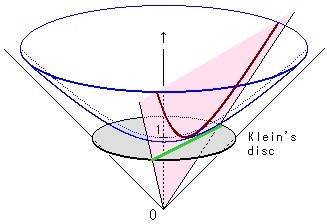
\includegraphics[scale=0.5]{Skice/ktop61.jpeg}
                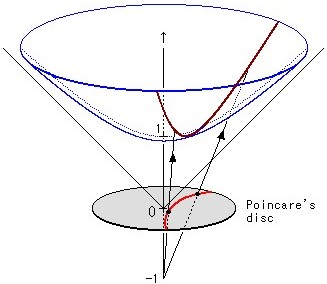
\includegraphics[scale=0.5]{Skice/ktop62.jpeg}
            \end{figure}
            
            Disk s središčem v $(0,0,1)$ in polmerom $1$, ki je tangenten na $\mathcal{H}$, si lahko predstavljamo kot Beltrami-Kleinov model hiperbolične geometrije.
           
            Izomorfizem med tema dvema modeloma (tj.\ injekcija med množicama, ki slika premice v premice) je podan s preslikavo, ki jo določajo presečišča premic skozi izhodišče  z diskom oziroma hiperboloidom. Preko tega izomorfizma lahko prenesemo skladnost/merjenje iz enega modela v drugega.
           
            Povezali bomo tudi Beltrami-Kleinov model in Poincaréjev model na disku in tako bo dovolj verificirati le Poincaréjev model na disku.


\section{Izometrija}

    Izometrija je taka preslikava, ki ohranja razdalje in kote.

    \begin{lema}
        Naj bo $\tilde{\mathcal{K}}=K(\tilde{S},\tilde{r})$ krožnica inverzije in naj bosta $A$ in $B$ različni točki, ki sta različni $\tilde{S}$.
        Potem je: $\frac{|A'B'|}{|AB|}=\frac{|\tilde{S}A'|}{|\tilde{S}B|}$, kjer sta $A'$ in $B'$ inverza točk $A$ in $B$ v $\tilde{\mathcal{K}}$.
    \end{lema}

        \begin{dokaz}
            \\ \begin{tikzpicture}
                % \clip (0,0) rectangle (14.000000,10.000000);
                {\footnotesize
                
                % Drawing circle k
                \draw [line width=0.016cm] (4.500000,3.500000) circle (1.802776);%
                
                % Drawing line s
                \draw [line width=0.016cm] (4.540000,3.500000) -- (5.660000,3.500000);%
                \draw [line width=0.016cm] (5.740000,3.500000) -- (7.168333,3.500000);%
                \draw [line width=0.016cm] (7.248333,3.500000) -- (8.000000,3.500000);%
                
                % Drawing line u
                \draw [line width=0.016cm] (7.208333,3.540000) -- (7.208333,4.460001);%

                % Drawing line S B'
                \draw [line width=0.016cm] (4.537523,3.513856) -- (5.518475,3.876099);%
                \draw [line width=0.016cm] (5.593522,3.903812) -- (7.170477,4.486144);%
                \draw [line width=0.016cm] (7.245523,4.513856) -- (8.000000,4.792467);%
                
                % Drawing segment B' A'
                \draw [line width=0.016cm] (5.569855,3.852432) -- (5.686144,3.537523);%
                
                % Marking point S by circle
                \draw [line width=0.016cm] (4.500000,3.500000) circle (0.040000);%
                \draw (4.530000,3.530000) node [anchor=north east] { $S$ };%
                
                % Marking point K
                \draw (3.000000,2.500000) node [anchor=east] { $\mathcal{K}$ };%

                % Marking point B by circle
                \draw [line width=0.016cm] (5.700000,3.500000) circle (0.040000);%
                \draw (5.670000,3.530000) node [anchor=north west] { $B$ };%
                
                % Marking point B' by circle
                \draw [line width=0.016cm] (7.208333,3.500000) circle (0.040000);%
                \draw (7.178333,3.530000) node [anchor=north west] { $B'$ };%
                
                % Marking point A' by circle
                \draw [line width=0.016cm] (7.208000,4.500000) circle (0.040000);%
                \draw (7.178000,4.530000) node [anchor=north west] { $A'$ };%
                
                % Marking point A by circle
                \draw [line width=0.016cm] (5.555999,3.889955) circle (0.040000);%
                \draw (5.555999,3.889955) node [anchor=south] { $A$ };%
                
                }
                \end{tikzpicture}
            \\ Po potenci točke na krožnico velja: $|\tilde{S}A|\cdot|\tilde{S}A'|=r^2=|\tilde{S}B|\cdot|\tilde{S}B'|$. Ker za trikotnika $\triangle\tilde{S}AB$ in $\triangle\tilde{S}B'A'$ velja razmerje $\frac{|\tilde{S}A|}{|\tilde{S}B|}=\frac{|\tilde{S}B'|}{|\tilde{S}A'|}$ in imata skupen kot pri $\tilde{S}$, potem po podobnostnem kriteriju SKS velja: $\triangle\tilde{S}AB\sim\triangle\tilde{S}B'A'$. Od tod pa sledi razmerje: $\frac{|A'B'|}{|AB|}=\frac{|\tilde{S}A'|}{|\tilde{S}B|}$
        \end{dokaz}

    \begin{trditev}
        Naj bo krožnica $\mathcal{K}=K(S,r)$ določa P-model hiperbolične ravnine in naj bi P-premica $p$ del krožnica $\tilde{\mathcal{K}}=K(\tilde{S},\tilde{r})$.
        Potem za poljubni točki $A,B\in\mathcal{H}$ velja $d(A,B)=d(A',B')$, kjer sta $A', B'$ inverza za točki $A, B$ v $\tilde{\mathcal{K}}$.
    \end{trditev}

        \begin{dokaz}
            \\ Naj bosta $\Omega$ in $\Sigma$ idealni točki na P-premici $\overleftrightarrow{AB}$ ter $\Omega'$ $\Sigma'$ njuni sliki pri inverziji v $\tilde{\mathcal{K}}$.
            \\ \begin{tikzpicture}
                    % \clip (0,0) rectangle (14.000000,10.000000);
                    {\footnotesize
                    
                    % Drawing circle k
                    \draw [line width=0.016cm] (2.000000,3.500000) circle (1.500000);%
                    
                    % Drawing circle k'
                    \draw [line width=0.016cm] (4.500000,3.500000) circle (2.000000);%
                    
                    % Marking point \tilde{S} by circle
                    \draw [line width=0.016cm] (2.000000,3.500000) circle (0.040000);%
                    \draw (2.000000,3.500000) node [anchor=east] { $\tilde{S}$ };%
                    
                    % Drawing arc S'' U 165.64
                    \draw [line width=0.016cm] (2.562500,3.003922) -- (2.569586,3.004866) arc (278:330:0.500000 and 0.500000) -- (2.935090,3.253633);%
                    \draw [line width=0.016cm] (2.963262,3.311883) -- (2.963592,3.312697) arc (338:360:0.500000 and 0.500000) --(3.000000,3.500000) arc (0:22:0.500000 and 0.500000) -- (2.960407,3.695001);%
                    \draw [line width=0.016cm] (2.928923,3.756954) -- (2.928584,3.757519) arc (31:82:0.500000 and 0.500000) -- (2.562500,3.996078);%
                    
                    % Marking point B' by circle
                    \draw [line width=0.016cm] (2.927000,3.717000) circle (0.040000);%
                    \draw (2.927000,3.717000) node [anchor=south] { $B'$ };%
                    
                    % Marking point A' by circle
                    \draw [line width=0.016cm] (2.928000,3.293000) circle (0.040000);%
                    \draw (2.928000,3.293000) node [anchor=north] { $A'$ };%
                    
                    % Marking point \Omega'
                    \draw (2.562000,3.996000) node [anchor=east] { $\Omega'$ };%
                    
                    % Marking point \Sigma'
                    \draw (2.562000,3.004000) node [anchor=east] { $\Sigma'$ };%
                    
                    % Marking point A by circle
                    \draw [line width=0.016cm] (5.097000,2.809000) circle (0.040000);%
                    \draw (5.097000,2.809000) node [anchor=east] { $A$ };%
                    
                    % Marking point B by circle
                    \draw [line width=0.016cm] (5.108000,4.228000) circle (0.040000);%
                    \draw (5.108000,4.228000) node [anchor=east] { $B$ };%
                    
                    % Marking point \Omega
                    \draw (5.625000,5.153595) node [anchor=west] { $\Omega$ };%
                    
                    % Marking point \Sigma
                    \draw (5.625000,1.846405) node [anchor=west] { $\Sigma$ };%
                    
                    % Drawing arc N \Omega 82.82
                    \draw [line width=0.016cm] (5.625000,5.153595) -- (5.613226,5.140148) arc (139:162:2.500000 and 2.500000) -- (5.120266,4.266073);%
                    \draw [line width=0.016cm] (5.096976,4.189549) -- (5.096846,4.189094) arc (164:195:2.500000 and 2.500000) -- (5.086618,2.847629);%
                    \draw [line width=0.016cm] (5.108723,2.770757) -- (5.109238,2.769071) arc (197:221:2.500000 and 2.500000) -- (5.624999,1.846406);%
                    
                    % Marking point S by circle
                    \draw [line width=0.016cm] (4.500000,3.500000) circle (0.040000);%
                    \draw (4.500000,3.500000) node [anchor=east] { $S$ };%
                    
                    % Marking point \mathcal{K}
                    \draw (6.100000,2.500000) node [anchor=north west] { $\mathcal{K}$ };%
                    
                    % Marking point \tilde{\mathcal{K}}
                    \draw (2.000000,2.000000) node [anchor=north] { $\tilde{\mathcal{K}}$ };%
                    }
                \end{tikzpicture}
            \\ Inverzija v $\tilde{\mathcal{K}}$ slika P-premico $\overleftrightarrow{AB}$ v P-premico $\overleftrightarrow{A'B'}$, saj inverzija slika premice in krožnicee v premice in krožnice ter ohranja velikosti kotov.
            \\ $d(A,B)=\left|\log(AB,\Omega\Sigma)\right|$ in $d(A',B')=\left|\log(A'B',\Omega'\Sigma')\right|$
            \\ Trdimo,da je \dashuline{$(AB,\Omega\Sigma)=(A'B',\Omega'\Sigma')$}, od tod pa sledi $d(A,B)=d(A',B')$.
            \\ $\frac{(AB,\Omega\Sigma)}{(A'B',\Omega'\Sigma')} \rightarrow \frac{\frac{|A'\Omega'|}{|A\Omega|}\cdot\frac{|B'\Sigma'|}{B\Sigma|}}{\frac{|A'\Sigma'|}{|A\Sigma|}\cdot\frac{|B'\Omega'|}{|B\Omega|}}$, po lemi je to enako: $\frac{\frac{|A'\tilde{S}|}{|\tilde{S}\Omega|}\cdot\frac{|B'\tilde{S}|}{\tilde{S}\Sigma|}}{\frac{|A'\tilde{S}|}{|\tilde{S}\Sigma|}\cdot\frac{|B'\tilde{S}|}{|\tilde{S}\Omega|}}=1$.
        \end{dokaz}

    \begin{posledica}
        Inverzija v $\tilde{\mathcal{K}}$ je izometrija $\mathcal{H}$, ki geometrijsko ustreza P-zrcaljenju v P-premici $\tilde{\mathcal{K}}\cap\mathcal{K}$.
    \end{posledica}

    \begin{trditev}
        Zrcaljenje v premici, ki je nosilka premera krožnice $\mathcal{K}$ porodi hiperbolično izometrijo, ki je hiperbolično zrcaljenje v tem premeru.
    \end{trditev}

    Podobno je rotacija s središčem v $S$ (središče $\mathcal{K}$) tudi hiperbolična izometrija.


    \section{Veljavnost aksiomov hiperbolične geometrije v Poincaréjev krožnem modelu}

            
    \subsection*{Aksiomi vsebovanosti}

        \begin{trditev}[V.1]
            Naj bosta $A,B\in\mathcal{H}$. Potem obstaja natanko ena $P$-premica skozi $A$ in $B$ v $\mathcal{H}$.
        \end{trditev}

            \begin{dokaz}
                \\ OBSTOJ:
                \begin{enumerate}
                    \item Če so $A, B, S$ evklidsko kolinearne, potem $A, B$ ležita na nekem premeru, ki je $P$-premica.
                    \item Če $A, B, S$ nisko evklidsko kolinearne. Naj bo $A'=inv_{\mathcal{K}}(A)$. Potem je vsaka krožnica, ki vsebuje $A$ in $A'$, pravokotna na $\mathcal{K}$. Ker $A, A', B$ niso kolinearne, enolično določajo krožnico $\tilde{\mathcal{K}}$, ki je pravokotna na $\mathcal{K}$. Potem je $\mathcal{K}\cap\tilde{\mathcal{K}}$~$P$-premica, ki vsebuje $A$ in $B$.
                \end{enumerate}
                ENOLIČNOST:
                \\ Naj za $A,B$ obstajata dve $P$-premici $p_1$ in $p_2$, ki ju vsebujeta. Ker dve točki enolično določata evklidsko premico, je največ ena izmed $p_1$ in $p_2$ lahko premer.
                \begin{enumerate}
                    \item Naj bo $p_1$ premer in $p_2$ krožni lok. Inverzija v $\mathcal{K}$ slika $A$ v $A'$ in $B$ v $B'$. Ker inverzija v $\mathcal{K}$ slika nosilko premera $p_1$ nazaj vase in krožnico $\tilde{\mathcal{K}}$, ki nosi $p_2$, prav tako nazaj vase, imata premica $p$ in krožnica $\tilde{\mathcal{K}}$ 4 skupne točke. Kar nas privede v protislovje.
                    \item $p_1$ in $p_2$ sta krožna loka. Kot zgoraj sledi, da imata krožnici, ki nosita $p_1$ in $p_2$, 4 skupne točke. Kar je spet protislovje.
                \end{enumerate}
            \end{dokaz}

        \begin{trditev}[V.2]
            Na vsaki $P$-premici ležita vsaj dve različni točki.
        \end{trditev}

        \begin{trditev}[V.3]
            Obstajajo tri različne nekolinearne točke.
        \end{trditev}

        Trditvi V.2 in V.3 očitno veljata.

    \subsection*{Aksiomi vmesnosti}

        \begin{trditev}[M.1]
            Če velja $A\ast B\ast C$, potem velja tudi $C\ast B\ast A$, kjer so $A, B, C$ različne kolinearne točke.
        \end{trditev}

        \begin{trditev}[M.2]
            Naj bosta $B,D\in\mathcal{H}$. Potem obstajajo točke $A,B,C\in\mathcal{H}$ na $P$-premici $AB$, da velja $A\ast B\ast D$, $B\ast C\ast D$ in $B \ast D \ast E$.
        \end{trditev}

        \begin{trditev}[M.3]
            Naj bodo $A,B,C\in\mathcal{H}$. Natanko ena točka leži med drugima dvema, če so točke kolinearne.
        \end{trditev}

        \begin{trditev}[M.4]
            Za poljubno $P$-premico $p$ in točke $A, B, C$, ki ne ležijo na $P$-premici $p$, velja:
            \begin{enumerate}
                \item Če sta $A$ in $B$ na istem bregu $P$-premice $p$ ter $B$ in $C$ na istem bregu $P$-premice $p$, potem sta $A$ in $C$ na istem bregu $P$-premice $p$.
                \item Če sta $A$ in $B$ na različnih bregovih $P$-premice $p$ in $B$ in $C$ na različnih bregovih $P$-premice $p$, potem sta $A$ in $C$ na istem bregu $P$-premice $p$.
            \end{enumerate}
        \end{trditev}
        \begin{dokaz}
            \\ Intuitivno je jasno, da vsaka $P$-premica razdeli $\mathcal{H}$ na dva bregova. Da uskladimo ta pojma, je treba dokazati, da intuitivna delitev ustreza uradni definiciji. Potem pa je verifikacija trditve M.4 dana. Argument za to je zelo podoben tistemu v dokazu trditve V.1.
        \end{dokaz}

    \subsection*{Aksiomi skladnosti}

        \begin{trditev}[S.1]
             Če sta $A$ in $B$ različni točki in $A'$ poljubna točka, potem na poljubnem poltraku $r$ z začetkom v $A'$ obstaja natanko ena točka $B'$, da velja $B'\neq A'$ in $AB\cong A'B'$.
        \end{trditev}

            \begin{dokaz}
                \\ Pokazati je treba, da ima poljuben poltrak neskončno dolžino.
                \\ Poltrak $r$ skozi $A$ je del neke P-premice. Pokazati moramo, da na $r$ obstaja taka točka $b$, da je $d(A,B)$ poljubno veliko. Naj bodo točke $A, \Omega, \Sigma$ fiksirane, $B$ pa lahko potuje od $A$ proti $\Omega$. Potem je: $\lim_{B\to\Omega}d(A,B)=\lim_{B\to\Omega}\left|\log\frac{|A\Omega|\cdot|B\Sigma|}{|A\Sigma|\cdot|B\Omega|}\right|=\infty$.
            \end{dokaz}

        \begin{trditev}[S.2]
            Skladnost daljic je ekvivalenčna relacija.
        \end{trditev}

        Trditev $S.2$ je očitna, saj je enakost, preko katere je definirana skladnost, ekvivalenčna relacija.

        \begin{trditev}[S.3]
            Če velja $A\ast B\ast C$, $A'\ast B'\ast C'$, $AB\cong A'B'$ in $BC\cong B'C'$, potem je $AC\cong A'C'$.
        \end{trditev}

            \begin{dokaz}
                \\ \begin{tikzpicture}
                        % \clip (0,0) rectangle (14.000000,10.000000);
                        {\footnotesize
                        
                        % Drawing circle l
                        \draw [line width=0.016cm] (4.500000,3.000000) circle (1.500000);%
                        
                        % Marking point B by circle
                        \draw [line width=0.016cm] (5.000000,3.000000) circle (0.040000);%
                        \draw (5.000000,3.000000) node [anchor=east] { $B$ };%
                        
                        % Marking point B' by circle
                        \draw [line width=0.016cm] (4.000000,3.000000) circle (0.040000);%
                        \draw (4.000000,3.000000) node [anchor=west] { $B'$ };%
                        
                        % Marking point \Omega
                        \draw (5.500000,4.118034) node [anchor=south west] { $\Omega$ };%
                        
                        % Marking point \Sigma
                        \draw (5.500000,1.881966) node [anchor=north west] { $\Sigma$ };%
                        
                        % Marking point \Omega'
                        \draw (3.500000,4.118034) node [anchor=south east] { $\Omega'$ };%
                        
                        % Marking point \Sigma'
                        \draw (3.500000,1.881966) node [anchor=north east] { $\Sigma'$ };%
                        
                        % Drawing arc P \Omega 96.38
                        \draw [line width=0.016cm] (5.500000,4.118034) -- (5.496304,4.114717) arc (132:158:1.500000 and 1.500000) -- (5.100075,3.538710);%
                        \draw [line width=0.016cm] (5.073436,3.463591) -- (5.073415,3.463526) arc (162:178:1.500000 and 1.500000) -- (5.000533,3.039996);%
                        \draw [line width=0.016cm] (5.000533,2.960004) -- (5.000914,2.947651) arc (182:198:1.500000 and 1.500000) -- (5.073436,2.536410);%
                        \draw [line width=0.016cm] (5.100074,2.461290) -- (5.109224,2.438090) arc (202:228:1.500000 and 1.500000) -- (5.500000,1.881966);%
                        
                        % Drawing arc P' \Sigma' 96.38
                        \draw [line width=0.016cm] (3.500000,1.881966) -- (3.503696,1.885282) arc (312:338:1.500000 and 1.500000) -- (3.899925,2.461289);%
                        \draw [line width=0.016cm] (3.926563,2.536409) -- (3.926585,2.536474) arc (342:358:1.500000 and 1.500000) -- (3.999467,2.960003);%
                        \draw [line width=0.016cm] (3.999467,3.039996) -- (3.999086,3.052349) arc (2:18:1.500000 and 1.500000) -- (3.926564,3.463591);%
                        \draw [line width=0.016cm] (3.899925,3.538710) -- (3.890776,3.561910) arc (22:48:1.500000 and 1.500000) -- (3.500000,4.118034);%
                        
                        % Marking point C' by circle
                        \draw [line width=0.016cm] (3.910000,3.500000) circle (0.040000);%
                        \draw (3.910000,3.500000) node [anchor=west] { $C'$ };%
                        
                        % Marking point A' by circle
                        \draw [line width=0.016cm] (3.910000,2.500000) circle (0.040000);%
                        \draw (3.910000,2.500000) node [anchor=west] { $A'$ };%
                        
                        % Marking point A by circle
                        \draw [line width=0.016cm] (5.090000,2.500000) circle (0.040000);%
                        \draw (5.090000,2.500000) node [anchor=east] { $A$ };%
                        
                        % Marking point C by circle
                        \draw [line width=0.016cm] (5.090000,3.500000) circle (0.040000);%
                        \draw (5.090000,3.500000) node [anchor=east] { $C$ };%
                        }
                    \end{tikzpicture}                    
                \\ $|AB|_H=|A'B'|_H=x$ in $|BC|_H=|B'C'|_H=y$. Dokazujemo: \dashuline{$|AB|_H+|BC|_H=|AC|_H$}.
                % \\ $|AC|_H=\left\lvert \log(AC, \Sigma\Omega)\right\rvert =\left\lvert \log\frac{|A\Sigma|\cdot|C\Omega|}{|A\Omega|\cdot|C\Sigma|}\right\rvert$
                \\ $|AB|_H+|BC|_H=\left\lvert \log\frac{|A\Sigma|\cdot|B\Omega|}{|A\Omega|\cdot|B\Sigma|}\right\rvert+\left\lvert \log\frac{|B\Sigma|\cdot|C\Omega|}{|B\Omega|\cdot|C\Sigma|}\right\rvert=\left\lvert \log\frac{|A\Sigma|\cdot|B\Omega|\cdot|B\Sigma|\cdot|C\Omega|}{|A\Omega|\cdot|B\Sigma|\cdot|C\Sigma|\cdot|B\Omega|}\right\rvert=\left\lvert \log\frac{|A\Sigma|\cdot|C\Omega|}{|A\Omega|\cdot|C\Sigma|}\right\rvert=|AC|_H$
                \\ Enak račun velja za $|A'C'|_H$.
            \end{dokaz}

        \begin{trditev}[S.4]
            Za dani kot $\angle CAB$ in dani poltrak $\overrightarrow{A'B'}$ obstaja natanko en poltrak $\overrightarrow{A'C'}$ na izbranem bregu $\overleftrightarrow{A'B'}$, da je $\angle CAB \cong \angle C'A'B'$.
        \end{trditev}

            \begin{dokaz}
                \\ Označimo: $|\angle CAB|=\alpha$ in glede na izbiro lege točke $A'$ ločimo $2$ primera:
                \\ (1): Če je $A'=O$, na izbranem bregu premice $\overleftrightarrow{A'B'}$ izbremo točko $C'$, ki z dano premico oklepa kot $\alpha$. (enako kot v evklidski geometriji)
                \\ (2): Če je $A'\neq O$. Naj bo $p$ evklidska premica, ki z $\overleftrightarrow{A'B'}$ oklepa  kot $\alpha$. Če je $p$ premer krožnice $\mathcal{K}$, je del premice $p$, ki leži v $\mathcal{H}$, iskana $P$-prmeica. 
                \\ \begin{tikzpicture}
                        % \clip (0,0) rectangle (14.000000,10.000000);
                        {\footnotesize
                        
                        % Drawing circle k
                        \draw [line width=0.016cm] (3.500000,3.500000) circle (2.000000);%
                        
                        % Marking point O by circle
                        \draw [line width=0.016cm] (3.500000,3.500000) circle (0.040000);%
                        \draw (3.500000,3.500000) node [anchor=east] { $O$ };%
                        
                        % Marking point p
                        \draw (3.500000,5.500000) node [anchor=south] { $p$ };%
                        
                        % Marking point A' by circle
                        \draw [line width=0.016cm] (4.000000,3.000000) circle (0.040000);%
                        \draw (4.000000,3.000000) node [anchor=west] { $A'$ };%
                        
                        % Drawing segment D p
                        \draw [line width=0.016cm] (4.269231,1.653846) -- (4.007845,2.960777);%
                        \draw [line width=0.016cm] (3.992155,3.039223) -- (3.500000,5.500000);%
                        
                        % Marking point \Sigma
                        \draw (4.122136,5.400775) node [anchor=south west] { $\Sigma$ };%
                        
                        % Marking point \Omega
                        \draw (4.524205,1.782152) node [anchor=north west] { $\Omega$ };%
                        
                        % Drawing segment O \Sigma
                        \draw [line width=0.016cm] (3.512443,3.538016) -- (4.122136,5.400775);%
                        
                        % Drawing segment O \Omega
                        \draw [line width=0.016cm] (3.520484,3.465643) -- (4.524205,1.782152);%
                        
                        % Marking point B' by circle
                        \draw [line width=0.016cm] (4.500000,3.970000) circle (0.040000);%
                        \draw (4.500000,3.970000) node [anchor=south] { $B'$ };%
                        
                        % Drawing arc S \Sigma 52.40
                        \draw [line width=0.016cm] (4.122136,5.400775) -- (4.101527,5.342352) arc (161:193:4.123106 and 4.123106) -- (3.990487,3.038852);%
                        \draw [line width=0.016cm] (4.009889,2.961243) -- (4.017386,2.932862) arc (195:212:4.123106 and 4.123106) -- (4.524205,1.782153);%
                        
                        % Drawing arc S' \Sigma' 96.46
                        \draw [line width=0.016cm] (5.236936,4.491490) -- (5.235950,4.491091) arc (112:136:2.039608 and 2.039608) -- (4.520739,4.004204);%
                        \draw [line width=0.016cm] (4.467811,3.946253) -- (4.460689,3.938103) arc (139:167:2.039608 and 2.039608) -- (4.008229,3.039144);%
                        \draw [line width=0.016cm] (3.992540,2.960702) -- (3.991378,2.954174) arc (170:208:2.039608 and 2.039608) -- (4.206406,1.628907);%
                        
                        % Marking point A by circle
                        \draw [line width=0.016cm] (5.800000,1.200000) circle (0.040000);%
                        \draw (5.800000,1.200000) node [anchor=south] { $A$ };%
                        
                        % Drawing segment O U
                        \draw [line width=0.016cm] (3.528284,3.471716) -- (3.971716,3.028284);%
                        \draw [line width=0.016cm] (4.028284,2.971716) -- (5.771716,1.228284);%
                        \draw [line width=0.016cm] (5.828284,1.171716) -- (6.000000,1.000000);%
                        
                        % Marking point S by circle
                        \draw [line width=0.016cm] (8.000000,4.000000) circle (0.040000);%
                        \draw (8.000000,4.000000) node [anchor=south] { $S$ };%
                        
                        % Drawing segment A' S
                        \draw [line width=0.016cm] (4.038806,3.009701) -- (4.145521,3.036380);%
                        \draw [line width=0.016cm] (4.218282,3.054571) -- (4.363803,3.090951);%
                        \draw [line width=0.016cm] (4.436564,3.109141) -- (4.582086,3.145521);%
                        \draw [line width=0.016cm] (4.654846,3.163712) -- (4.800368,3.200092);%
                        \draw [line width=0.016cm] (4.873128,3.218282) -- (5.018650,3.254662);%
                        \draw [line width=0.016cm] (5.091410,3.272853) -- (5.236932,3.309233);%
                        \draw [line width=0.016cm] (5.309692,3.327423) -- (5.455214,3.363803);%
                        \draw [line width=0.016cm] (5.527974,3.381994) -- (5.673496,3.418374);%
                        \draw [line width=0.016cm] (5.746257,3.436564) -- (5.891778,3.472944);%
                        \draw [line width=0.016cm] (5.964539,3.491135) -- (6.110060,3.527515);%
                        \draw [line width=0.016cm] (6.182821,3.545705) -- (6.328342,3.582086);%
                        \draw [line width=0.016cm] (6.401103,3.600276) -- (6.546624,3.636656);%
                        \draw [line width=0.016cm] (6.619385,3.654846) -- (6.764906,3.691227);%
                        \draw [line width=0.016cm] (6.837667,3.709417) -- (6.983188,3.745797);%
                        \draw [line width=0.016cm] (7.055949,3.763987) -- (7.201470,3.800368);%
                        \draw [line width=0.016cm] (7.274231,3.818558) -- (7.419752,3.854938);%
                        \draw [line width=0.016cm] (7.492513,3.873128) -- (7.638034,3.909509);%
                        \draw [line width=0.016cm] (7.710795,3.927699) -- (7.856316,3.964079);%
                        \draw [line width=0.016cm] (7.929077,3.982269) -- (7.961194,3.990299);%
                        
                        % Drawing segment A S
                        \draw [line width=0.016cm] (5.824713,1.231453) -- (5.892673,1.317948);%
                        \draw [line width=0.016cm] (5.939010,1.376922) -- (6.031683,1.494869);%
                        \draw [line width=0.016cm] (6.078020,1.553843) -- (6.170693,1.671791);%
                        \draw [line width=0.016cm] (6.217030,1.730765) -- (6.309703,1.848713);%
                        \draw [line width=0.016cm] (6.356039,1.907687) -- (6.448713,2.025634);%
                        \draw [line width=0.016cm] (6.495049,2.084608) -- (6.587722,2.202556);%
                        \draw [line width=0.016cm] (6.634059,2.261530) -- (6.726732,2.379478);%
                        \draw [line width=0.016cm] (6.773069,2.438451) -- (6.865742,2.556399);%
                        \draw [line width=0.016cm] (6.912079,2.615373) -- (7.004752,2.733321);%
                        \draw [line width=0.016cm] (7.051089,2.792295) -- (7.143762,2.910242);%
                        \draw [line width=0.016cm] (7.190098,2.969216) -- (7.282772,3.087164);%
                        \draw [line width=0.016cm] (7.329108,3.146138) -- (7.421782,3.264086);%
                        \draw [line width=0.016cm] (7.468118,3.323060) -- (7.560791,3.441007);%
                        \draw [line width=0.016cm] (7.607128,3.499981) -- (7.699801,3.617929);%
                        \draw [line width=0.016cm] (7.746138,3.676903) -- (7.838811,3.794851);%
                        \draw [line width=0.016cm] (7.885148,3.853824) -- (7.975287,3.968547);%
                        
                        % Marking point \mathcal{K}
                        \draw (3.500000,1.300000) node  { $\mathcal{K}$ };%

                        % Marking point \tilde{\mathcal{K}}
                        \draw (4.000000,4.100000) node  { $\tilde{\mathcal{K}}$ };%
                        }
                    \end{tikzpicture}                    
                \\ Sicer moramo poiskati krožnico ima premico $p$ za tangento in seka krožnico $\mathcal{K}$ pravokotno. Središče iskane krožnice leži na pravokotnici skozi točko $A'$ na premico $p$. Naj bo $A=inv_{\mathcal{K}}(A')$ in $S$ presečišče pravokotnice na $p$ skozi $A'$ in daljice $AA'$. Po definiciji inverzije je $|OA'|\cdot|OA|=1$. Potenca točke na krožnico nam da: $\mathcal{P}_{\tilde{\mathcal{K}}}(O)=1=|O\Sigma|^2=|O\Omega|^2$. Potem sta $\overleftrightarrow{O\Sigma}$ in $\overleftrightarrow{O\Omega}$ tangentni na krožnico $\tilde{\mathcal{K}}$.
            \end{dokaz}
        
        \begin{trditev}[S.5]
            Skladnost kotov je ekvivalenčna relacija.
        \end{trditev}

        Trditev $S.5$ je očitna, saj je enakost, preko katere je definirana skladnost, ekvivalenčna relacija.

        \begin{trditev}[S.6/SKS]
             Če sta stranici in vmesni kot enega trikotnika skladni s stranicama in vmesnim kotom drugega trikotnika, potem sta trikotnika skladna.
        \end{trditev}

        To trditev bomo preverili tako, da bomo poljuben trikotnik prestavili v posebno lego.
         
        Način, kako trikotnik prestavimo, mora biti tak, da bo P-premice slikal v P-premice in da bo ohranjal razdalje in kote -- izometrija. 
        \\ To lahko storimo z inverzijo v poljubni krožnici $\tilde{\mathcal{K}}$, ki je pravokotna na $\mathcal{K}$.
        $inv_{\tilde{\mathcal{K}}}$ porodi bijekcijo $\mathcal{H}\to\mathcal{H}$, ki fiksira točke na P-premici $\tilde{\mathcal{K}}\cap\mathcal{K}$. To bo hiperbolično zrcaljenje. 
        \\ Preveriti je potrebno še, da ohranja P-dolžino. Poleg prej obravnavanih izometrij, lahko uporabimo tudi evklidske izometrije, če le-te ohranjajo množico $\mathcal{H}$. Vsaka taka porodi bijekcijo $\mathcal{H}\to\mathcal{H}$, ki ohranja velikosti kotov in evklidske razdalje, zato pa posledično ohranja hiperbolične razdalje.
        \\ Z uporabo teh izometrij bomo poljuben P-trikotnik preslikali na skladen trikotnik v odlikovani legi.
        

            \begin{dokaz}
                \\ Naj bo $\triangle ABC$ poljuben P-trikotnik. (trikotnik preslikamo v skladen trikotnik $\triangle SB'C'$) 
                \\ \begin{tikzpicture}
                        % \clip (0,0) rectangle (14.000000,10.000000);
                        {\footnotesize
                        
                        % Marking point S by circle
                        \draw [line width=0.016cm] (3.000000,3.000000) circle (0.040000);%
                        \draw (3.000000,3.000000) node [anchor=north] { $S$ };%
                        
                        % Drawing circle k
                        \draw [line width=0.016cm] (3.000000,3.000000) circle (1.500000);%
                        
                        % Marking point A by circle
                        \draw [line width=0.016cm] (3.700000,3.200000) circle (0.040000);%
                        \draw (3.700000,3.200000) node [anchor=north] { $A$ };%
                        
                        % Marking point M by circle
                        \draw [line width=0.016cm] (3.350000,3.100000) circle (0.040000);%
                        \draw (3.380000,3.070000) node [anchor=south east] { $M$ };%
                        
                        % Marking point \Sigma
                        \draw (1.557714,2.587918) node [anchor=east] { $\Sigma$ };%
                        
                        % Marking point \Omega
                        \draw (4.442286,3.412082) node [anchor=west] { $\Omega$ };%
                        
                        % Marking point M' by circle
                        \draw [line width=0.016cm] (6.500000,4.000000) circle (0.040000);%
                        \draw (6.470000,3.970000) node [anchor=south west] { $M'$ };%
                        
                        % Drawing circle k'
                        \draw [line width=0.016cm] (6.563025,3.549999) arc (360:360:1.638025 and 1.638025) --(6.563025,3.550000) arc (0:14:1.638025 and 1.638025) -- (6.510518,3.961408);%
                        \draw [line width=0.016cm] (6.488542,4.038324) -- (6.482854,4.056177) arc (18:194:1.638025 and 1.638025) -- (3.339481,3.138593);%
                        \draw [line width=0.016cm] (3.361457,3.061677) -- (3.367146,3.043823) arc (198:359:1.638025 and 1.638025) -- (6.563025,3.549999);%
                        
                        % Marking point C by circle
                        \draw [line width=0.016cm] (3.800000,3.700000) circle (0.040000);%
                        \draw (3.800000,3.700000) node [anchor=south] { $C$ };%
                        
                        % Marking point B by circle
                        \draw [line width=0.016cm] (4.200000,2.900000) circle (0.040000);%
                        \draw (4.200000,2.900000) node [anchor=north] { $B$ };%
                        
                        % Drawing Bezier curve A X C
                        \draw [line width=0.016cm] (3.720988,3.245679) -- (3.716926,3.236243);%
                        \draw [line width=0.016cm] (3.725849,3.257485) -- (3.720988,3.245679);%
                        \draw [line width=0.016cm] (3.730556,3.269444) -- (3.725849,3.257485);%
                        \draw [line width=0.016cm] (3.735108,3.281559) -- (3.730556,3.269444);%
                        \draw [line width=0.016cm] (3.739506,3.293827) -- (3.735108,3.281559);%
                        \draw [line width=0.016cm] (3.743750,3.306250) -- (3.739506,3.293827);%
                        \draw [line width=0.016cm] (3.747840,3.318827) -- (3.743750,3.306250);%
                        \draw [line width=0.016cm] (3.751775,3.331559) -- (3.747840,3.318827);%
                        \draw [line width=0.016cm] (3.755556,3.344444) -- (3.751775,3.331559);%
                        \draw [line width=0.016cm] (3.759182,3.357485) -- (3.755556,3.344444);%
                        \draw [line width=0.016cm] (3.762654,3.370679) -- (3.759182,3.357485);%
                        \draw [line width=0.016cm] (3.765972,3.384028) -- (3.762654,3.370679);%
                        \draw [line width=0.016cm] (3.769136,3.397531) -- (3.765972,3.384028);%
                        \draw [line width=0.016cm] (3.772145,3.411188) -- (3.769136,3.397531);%
                        \draw [line width=0.016cm] (3.775000,3.425000) -- (3.772145,3.411188);%
                        \draw [line width=0.016cm] (3.777701,3.438966) -- (3.775000,3.425000);%
                        \draw [line width=0.016cm] (3.780247,3.453086) -- (3.777701,3.438966);%
                        \draw [line width=0.016cm] (3.782639,3.467361) -- (3.780247,3.453086);%
                        \draw [line width=0.016cm] (3.784877,3.481790) -- (3.782639,3.467361);%
                        \draw [line width=0.016cm] (3.786960,3.496373) -- (3.784877,3.481790);%
                        \draw [line width=0.016cm] (3.788889,3.511111) -- (3.786960,3.496373);%
                        \draw [line width=0.016cm] (3.790664,3.526003) -- (3.788889,3.511111);%
                        \draw [line width=0.016cm] (3.792284,3.541049) -- (3.790664,3.526003);%
                        \draw [line width=0.016cm] (3.793750,3.556250) -- (3.792284,3.541049);%
                        \draw [line width=0.016cm] (3.795062,3.571605) -- (3.793750,3.556250);%
                        \draw [line width=0.016cm] (3.796219,3.587114) -- (3.795062,3.571605);%
                        \draw [line width=0.016cm] (3.797222,3.602778) -- (3.796219,3.587114);%
                        \draw [line width=0.016cm] (3.798071,3.618596) -- (3.797222,3.602778);%
                        \draw [line width=0.016cm] (3.798765,3.634568) -- (3.798071,3.618596);%
                        \draw [line width=0.016cm] (3.799306,3.650694) -- (3.798765,3.634568);%
                        \draw [line width=0.016cm] (3.799526,3.660003) -- (3.799306,3.650694);%
                        
                        % Drawing Bezier curve A Y B
                        \draw [line width=0.016cm] (3.745679,3.196296) -- (3.739895,3.197101);%
                        \draw [line width=0.016cm] (3.757485,3.194213) -- (3.745679,3.196296);%
                        \draw [line width=0.016cm] (3.769444,3.191667) -- (3.757485,3.194213);%
                        \draw [line width=0.016cm] (3.781559,3.188657) -- (3.769444,3.191667);%
                        \draw [line width=0.016cm] (3.793827,3.185185) -- (3.781559,3.188657);%
                        \draw [line width=0.016cm] (3.806250,3.181250) -- (3.793827,3.185185);%
                        \draw [line width=0.016cm] (3.818827,3.176852) -- (3.806250,3.181250);%
                        \draw [line width=0.016cm] (3.831559,3.171991) -- (3.818827,3.176852);%
                        \draw [line width=0.016cm] (3.844444,3.166667) -- (3.831559,3.171991);%
                        \draw [line width=0.016cm] (3.857485,3.160880) -- (3.844444,3.166667);%
                        \draw [line width=0.016cm] (3.870679,3.154630) -- (3.857485,3.160880);%
                        \draw [line width=0.016cm] (3.884028,3.147917) -- (3.870679,3.154630);%
                        \draw [line width=0.016cm] (3.897531,3.140741) -- (3.884028,3.147917);%
                        \draw [line width=0.016cm] (3.911188,3.133102) -- (3.897531,3.140741);%
                        \draw [line width=0.016cm] (3.925000,3.125000) -- (3.911188,3.133102);%
                        \draw [line width=0.016cm] (3.938966,3.116435) -- (3.925000,3.125000);%
                        \draw [line width=0.016cm] (3.953086,3.107407) -- (3.938966,3.116435);%
                        \draw [line width=0.016cm] (3.967361,3.097917) -- (3.953086,3.107407);%
                        \draw [line width=0.016cm] (3.981790,3.087963) -- (3.967361,3.097917);%
                        \draw [line width=0.016cm] (3.996373,3.077546) -- (3.981790,3.087963);%
                        \draw [line width=0.016cm] (4.011111,3.066667) -- (3.996373,3.077546);%
                        \draw [line width=0.016cm] (4.026003,3.055324) -- (4.011111,3.066667);%
                        \draw [line width=0.016cm] (4.041049,3.043519) -- (4.026003,3.055324);%
                        \draw [line width=0.016cm] (4.056250,3.031250) -- (4.041049,3.043519);%
                        \draw [line width=0.016cm] (4.071605,3.018519) -- (4.056250,3.031250);%
                        \draw [line width=0.016cm] (4.087114,3.005324) -- (4.071605,3.018519);%
                        \draw [line width=0.016cm] (4.102778,2.991667) -- (4.087114,3.005324);%
                        \draw [line width=0.016cm] (4.118596,2.977546) -- (4.102778,2.991667);%
                        \draw [line width=0.016cm] (4.134568,2.962963) -- (4.118596,2.977546);%
                        \draw [line width=0.016cm] (4.150694,2.947917) -- (4.134568,2.962963);%
                        \draw [line width=0.016cm] (4.166975,2.932407) -- (4.150694,2.947917);%
                        \draw [line width=0.016cm] (4.171471,2.928038) -- (4.166975,2.932407);%
                        
                        % Drawing Bezier curve C Z B
                        \draw [line width=0.016cm] (3.811728,3.655556) -- (3.810169,3.661314);%
                        \draw [line width=0.016cm] (3.818056,3.633333) -- (3.811728,3.655556);%
                        \draw [line width=0.016cm] (3.824691,3.611111) -- (3.818056,3.633333);%
                        \draw [line width=0.016cm] (3.831636,3.588889) -- (3.824691,3.611111);%
                        \draw [line width=0.016cm] (3.838889,3.566667) -- (3.831636,3.588889);%
                        \draw [line width=0.016cm] (3.846451,3.544444) -- (3.838889,3.566667);%
                        \draw [line width=0.016cm] (3.854321,3.522222) -- (3.846451,3.544444);%
                        \draw [line width=0.016cm] (3.862500,3.500000) -- (3.854321,3.522222);%
                        \draw [line width=0.016cm] (3.870988,3.477778) -- (3.862500,3.500000);%
                        \draw [line width=0.016cm] (3.879784,3.455556) -- (3.870988,3.477778);%
                        \draw [line width=0.016cm] (3.888889,3.433333) -- (3.879784,3.455556);%
                        \draw [line width=0.016cm] (3.898302,3.411111) -- (3.888889,3.433333);%
                        \draw [line width=0.016cm] (3.908025,3.388889) -- (3.898302,3.411111);%
                        \draw [line width=0.016cm] (3.918056,3.366667) -- (3.908025,3.388889);%
                        \draw [line width=0.016cm] (3.928395,3.344444) -- (3.918056,3.366667);%
                        \draw [line width=0.016cm] (3.939043,3.322222) -- (3.928395,3.344444);%
                        \draw [line width=0.016cm] (3.950000,3.300000) -- (3.939043,3.322222);%
                        \draw [line width=0.016cm] (3.961265,3.277778) -- (3.950000,3.300000);%
                        \draw [line width=0.016cm] (3.972840,3.255556) -- (3.961265,3.277778);%
                        \draw [line width=0.016cm] (3.984722,3.233333) -- (3.972840,3.255556);%
                        \draw [line width=0.016cm] (3.996914,3.211111) -- (3.984722,3.233333);%
                        \draw [line width=0.016cm] (4.009414,3.188889) -- (3.996914,3.211111);%
                        \draw [line width=0.016cm] (4.022222,3.166667) -- (4.009414,3.188889);%
                        \draw [line width=0.016cm] (4.035340,3.144444) -- (4.022222,3.166667);%
                        \draw [line width=0.016cm] (4.048765,3.122222) -- (4.035340,3.144444);%
                        \draw [line width=0.016cm] (4.062500,3.100000) -- (4.048765,3.122222);%
                        \draw [line width=0.016cm] (4.076543,3.077778) -- (4.062500,3.100000);%
                        \draw [line width=0.016cm] (4.090895,3.055556) -- (4.076543,3.077778);%
                        \draw [line width=0.016cm] (4.105556,3.033333) -- (4.090895,3.055556);%
                        \draw [line width=0.016cm] (4.120525,3.011111) -- (4.105556,3.033333);%
                        \draw [line width=0.016cm] (4.135802,2.988889) -- (4.120525,3.011111);%
                        \draw [line width=0.016cm] (4.151389,2.966667) -- (4.135802,2.988889);%
                        \draw [line width=0.016cm] (4.167284,2.944444) -- (4.151389,2.966667);%
                        \draw [line width=0.016cm] (4.176232,2.932173) -- (4.167284,2.944444);%
                        
                        % Drawing segment \Sigma U
                        \draw [line width=0.016cm] (1.557714,2.587918) -- (2.961539,2.989011);%
                        \draw [line width=0.016cm] (3.038461,3.010989) -- (3.311539,3.089011);%
                        \draw [line width=0.016cm] (3.388461,3.110989) -- (3.661539,3.189011);%
                        \draw [line width=0.016cm] (3.738461,3.210989) -- (6.461539,3.989011);%
                        \draw [line width=0.016cm] (6.538461,4.010989) -- (7.000000,4.142857);%
                        
                        % Marking point \mathcal{K}
                        \draw (3.000000,4.500000) node [anchor=south] { $\mathcal{K}$ };%
                        
                        % Marking point \tilde{\mathcal{K}}
                        \draw (5.000000,2.000000) node [anchor=north] { $\tilde{\mathcal{K}}$ };%
                        }
                    \end{tikzpicture}
                \\ Naj bo $M$ razpolovišče daljice $SA$, torej tista točka na evklidski premici $\overleftrightarrow{SA}$, za katero je $d(SM)=\frac{1}{2}d(SA)$. Da določimo $M$, moramo evklidsko razdlajo $|SM|=d$ izraziti s pomočjo evklidske dolžine $|SA|=a$. Z upoštevanjem $|S\Omega|=|S\Sigma|=r$ (polmer $\mathcal{K}$) dobimo: $|A\Omega|=r-a;~|A\Sigma|=r+a;~|M\Omega|=r-d;~|M\Sigma|=r+d$. Velja: $\left| \log(SM,\Omega\Sigma)\right|=d(SM)=\frac{1}{2}d(SA)=\frac{1}{2}\left|\log(SA,\Omega\Sigma)\right|$. Zaradi izbire $\Omega$ in $\Sigma$ lahko izpustimo absolutno vrednost $|\cdot|$, nato antilogaritmiramo in dobimo: $(SA,\Omega\Sigma)=(SM,\Omega\Sigma)^2$. To enakost lahko poračunamo:
                \\ \begin{align*}
                \frac{r+a}{r-a}&=\left( \frac{r+d}{r-d}\right)^2  ~~/d=ka\\
                \frac{r+a}{r-a}&=\left( \frac{r+ka}{r-ka}\right)^2 \\
                (r+a)(r-ka)^2&=(r-a)(r+ka)^2 \\
                2r^2a+2k^2a^3-4akr^2&=0  ~~/:2a \\
                a^2k^2-2kr^2+r^2&=0  ~~/:a^2 \\
                k^2-2k\left(\frac{r}{a}\right)^2+\left(\frac{r}{a}\right)^2&=0
                \end{align*}
                Od tod sledi $k=\left(\frac{r}{a}\right)^2\left( 1 \pm \sqrt{1-\left(\frac{a}{r}\right)^2} \right)$. Ker pa mora glede na hiperbolično razdaljo veljati $\frac{1}{2}<k<1$, potem sledi, da je $k=\left(\frac{r}{a}\right)^2\left( 1 - \sqrt{1-\left(\frac{a}{r}\right)^2} \right)$. Z uporabo razvoja v vrsto, dobimo $k=\frac{1}{2}+\frac{1}{8}\left(\frac{a}{r}\right)^2+\cdots$.
                \\ Naj bo $M'$ inverz točke $M$ v $\mathcal{K}$ in $\tilde{\mathcal{K}}$ krožnica s premerom $MM'$. Potem je $\mathcal{K}\perp\tilde{\mathcal{K}}$, in ker je inverzija v $\mathcal{K}$ izometrija $\mathcal{H}$, preslika točko $A$ v točko $S$. Označimo s $C'$ in $B'$ inverza točk $C$ in $B$ v $\tilde{\mathcal{K}}$. Potem velja naslednja P-skladnost $\triangle SB'C'\sim\triangle ABC$.
                \\ Z vrtenjem okoli točke $S$ lahko točko $B'$ spravimo na pozitivni poltrak vodoravne osi skozi $S$. Če slika $C'$ pri tem pristane v spodnji polravnini, uporabimo še evklidsko zrcaljenje v vodoravnem premeru, da jo preslikamo v zgornjo polravnino. Tako dobimo P-trikotnik $\triangle SB''C''$, ki je P-skladen s trikotnikom $\triangle ABC$.
                \\ \begin{tikzpicture}
                        % \clip (0,0) rectangle (14.000000,10.000000);
                        {\footnotesize
                        
                        % Marking point S by circle
                        \draw [line width=0.016cm] (3.000000,3.000000) circle (0.040000);%
                        \draw (3.000000,3.000000) node [anchor=north] { $S$ };%
                        
                        % Drawing circle k
                        \draw [line width=0.016cm] (3.000000,3.000000) circle (1.500000);%
                        
                        % Drawing line b
                        \draw [line width=0.016cm] (1.300000,3.000000) -- (2.960000,3.000000);%
                        \draw [line width=0.016cm] (3.040000,3.000000) -- (3.960000,3.000000);%
                        \draw [line width=0.016cm] (4.040000,3.000000) -- (4.700000,3.000000);%
                        
                        % Drawing segment S C
                        \draw [line width=0.016cm] (2.977812,3.033282) -- (2.404188,3.893718);%
                        \draw [line width=0.016cm] (2.359812,3.960282) -- (2.000000,4.500000);%
                        
                        % Marking point C'=F' by circle
                        \draw [line width=0.016cm] (2.382000,3.927000) circle (0.040000);%
                        \draw (2.352000,3.897000) node [anchor=south west] { $C'=F'$ };%
                        
                        % Marking point B'=E' by circle
                        \draw [line width=0.016cm] (4.000000,3.000000) circle (0.040000);%
                        \draw (4.000000,3.000000) node [anchor=north] { $B'=E'$ };%
                        
                        % Drawing segment C'=F' B'=E'
                        \draw [line width=0.016cm] (2.416707,3.907115) -- (3.965293,3.019885);%
                        }
                    \end{tikzpicture}                    
                \\ Če je za nek trikotnik $\triangle DEF$ velja: $\triangle DEF\cong\triangle ABC$, potem ga lahko na enak način preslikamo v trikotnik $\triangle SE'F'$. Velja: $SE'\cong DE\cong AB\cong SB'' \Rightarrow E'=B''$. Ker za kota velja $\angle D\cong \angle A$, sta v trikotnikih $\triangle SB''C''$ in $\triangle SE'F'$ skladna kota pri $S$, zato za poltraka velja: $\overrightarrow{SC''}=\overrightarrow{SF'}$ in kot prej velja $SC''\cong SF' \Rightarrow C''=F'$. To pomeni, da soupadata tudi daljici $B''C''$ in $E'F'$ v teh trikotnikih. Sklep: $\triangle ABC \cong \triangle SB''C''\cong \triangle SE'F'\cong \triangle DEF$.
            \end{dokaz}

        \begin{posledica}
           Dva P-trikotnika sta skladna natanko tedaj, ko obstaja izometrija, ki enega preslika na drugega.
           Ta izometrija je kompozitum P-zrcaljenj (= inverzije v P-premicah), evklidskih zrcaljenj v premerih $\mathcal{K}$ in vrtenj okoli središča $\mathcal{K}$.
        \end{posledica}

\section{Kot vzporednosti v Poincaréjevem modelu}

    \begin{izrek}
        V Poincaréjevem modelu za kot vzporednosti velja: $\tan\left(\frac{\Pi(d)}{2}\right)=e^{-d}$, kjer je $d=d(A,p)$.
    \end{izrek}

        \begin{dokaz}
            \\ Za dano premico $p$ in točko $A\notin p$ asimptotična poltraka iz $A$ oklepata s pravokotnico iz $A$ na $p$ kot, ki ga imenujemo kot vzporednosti $\Pi(A,p)$. Pokazali smo že, da je ta odvisen le od oddaljenosti $A$ od $p$. Naj bo $d=d(AA')$ in $\Pi(A,p)=\Pi(d)$, kjer je $A'$ pravokotna projekcija $A$ na $p$. $\Pi(d)$ bomo izračunali tako, da bomo izbrali posebno lego za $p$ in $A$.
            \\ Naj bo $p$ premer $\mathcal{K}$ in $A$ nad $S$ taka točka, da je $d(AS)=d$. Asimptotičen poltrak skozi $A$ k $p$ je krožni lok na krožnici $\tilde{\mathcal{K}}$ skozi $A$ in $\Omega$, ki je v $\Omega$ pravokoten na $\mathcal{K}$. Središče $\tilde{S}$ krožnice $\tilde{\mathcal{K}}$ je presečišče simetrale daljice $A\Omega$ in pravokotnice na $p$ v $\Omega$.
            \\ \begin{tikzpicture}
                    % \clip (0,0) rectangle (14.000000,10.000000);
                    {\footnotesize
                    
                    % Drawing circle k
                    \draw [line width=0.016cm] (3.500000,3.500000) circle (2.000000);%
                    
                    % Marking point S by circle
                    \draw [line width=0.016cm] (3.500000,3.500000) circle (0.040000);%
                    \draw (3.500000,3.500000) node [anchor=north] { $S$ };%
                    
                    % Marking point \Sigma
                    \draw (1.500000,3.500000) node [anchor=east] { $\Sigma$ };%
                    
                    % Marking point \Omega
                    \draw (5.500000,3.500000) node [anchor=west] { $\Omega$ };%
                    
                    % Marking point \tilde{S} by circle
                    \draw [line width=0.016cm] (5.500000,6.500000) circle (0.040000);%
                    \draw (5.500000,6.500000) node [anchor=west] { $\tilde{S}$ };%
                    
                    % Drawing circle k'
                    \draw [line width=0.016cm] (2.501667,6.600000) -- (2.500457,6.552358) arc (179:227:3.000000 and 3.000000) -- (3.470364,4.290797);%
                    \draw [line width=0.016cm] (3.529991,4.237465) -- (3.531822,4.235872) arc (229:279:3.000000 and 3.000000) -- (5.999998,3.541960);%
                    
                    % Marking point A by circle
                    \draw [line width=0.016cm] (3.500000,4.263932) circle (0.040000);%
                    \draw (3.500000,4.263932) node [anchor=east] { $A$ };%
                    
                    % Drawing segment S X
                    \draw [line width=0.016cm] (3.500000,3.540000) -- (3.500000,4.223932);%
                    \draw [line width=0.016cm] (3.500000,4.303932) -- (3.500000,6.600000);%
                    
                    % Drawing line q'
                    \draw [line width=0.016cm] (1.300000,6.231672) -- (3.470186,4.290599);%
                    \draw [line width=0.016cm] (3.529814,4.237265) -- (4.324288,3.526667);%
                    \draw [line width=0.016cm] (4.383916,3.473333) -- (6.000000,2.027864);%
                    
                    % Drawing segment \Sigma \Omega
                    \draw [line width=0.016cm] (1.500000,3.500000) -- (3.460000,3.500000);%
                    \draw [line width=0.016cm] (3.540000,3.500000) -- (4.314102,3.500000);%
                    \draw [line width=0.016cm] (4.394102,3.500000) -- (5.500000,3.500000);%
                    
                    % Marking point M by circle
                    \draw [line width=0.016cm] (4.354102,3.500000) circle (0.040000);%
                    \draw (4.354102,3.500000) node [anchor=north] { $M$ };%
                    
                    % Drawing segment \tilde{S} A
                    \draw [line width=0.016cm] (5.473333,6.470186) -- (5.400000,6.388197);%
                    \draw [line width=0.016cm] (5.350000,6.332295) -- (5.250000,6.220492);%
                    \draw [line width=0.016cm] (5.200000,6.164590) -- (5.100000,6.052786);%
                    \draw [line width=0.016cm] (5.050000,5.996885) -- (4.950000,5.885081);%
                    \draw [line width=0.016cm] (4.900000,5.829180) -- (4.800000,5.717376);%
                    \draw [line width=0.016cm] (4.750000,5.661475) -- (4.650000,5.549671);%
                    \draw [line width=0.016cm] (4.600000,5.493769) -- (4.500000,5.381966);%
                    \draw [line width=0.016cm] (4.450000,5.326064) -- (4.350000,5.214261);%
                    \draw [line width=0.016cm] (4.300000,5.158359) -- (4.200000,5.046556);%
                    \draw [line width=0.016cm] (4.150000,4.990654) -- (4.050000,4.878851);%
                    \draw [line width=0.016cm] (4.000000,4.822949) -- (3.900000,4.711146);%
                    \draw [line width=0.016cm] (3.850000,4.655244) -- (3.750000,4.543441);%
                    \draw [line width=0.016cm] (3.700000,4.487539) -- (3.600000,4.375735);%
                    \draw [line width=0.016cm] (3.550000,4.319834) -- (3.526667,4.293746);%
                    
                    % Drawing segment \tilde{S} \Omega
                    \draw [line width=0.016cm] (5.500000,6.460000) -- (5.500000,6.350000);%
                    \draw [line width=0.016cm] (5.500000,6.275000) -- (5.500000,6.125000);%
                    \draw [line width=0.016cm] (5.500000,6.050000) -- (5.500000,5.900000);%
                    \draw [line width=0.016cm] (5.500000,5.825000) -- (5.500000,5.675000);%
                    \draw [line width=0.016cm] (5.500000,5.600000) -- (5.500000,5.450000);%
                    \draw [line width=0.016cm] (5.500000,5.375000) -- (5.500000,5.225000);%
                    \draw [line width=0.016cm] (5.500000,5.150000) -- (5.500000,5.000000);%
                    \draw [line width=0.016cm] (5.500000,4.925000) -- (5.500000,4.775000);%
                    \draw [line width=0.016cm] (5.500000,4.700000) -- (5.500000,4.550000);%
                    \draw [line width=0.016cm] (5.500000,4.475000) -- (5.500000,4.325000);%
                    \draw [line width=0.016cm] (5.500000,4.250000) -- (5.500000,4.100000);%
                    \draw [line width=0.016cm] (5.500000,4.025000) -- (5.500000,3.875000);%
                    \draw [line width=0.016cm] (5.500000,3.800000) -- (5.500000,3.650000);%
                    \draw [line width=0.016cm] (5.500000,3.575000) -- (5.500000,3.500000);%
                    
                    % Drawing segment \tilde{S} M
                    \draw [line width=0.016cm] (5.485727,6.462633) -- (5.446477,6.359874);%
                    \draw [line width=0.016cm] (5.419715,6.289811) -- (5.366192,6.149685);%
                    \draw [line width=0.016cm] (5.339430,6.079622) -- (5.285907,5.939497);%
                    \draw [line width=0.016cm] (5.259145,5.869434) -- (5.205622,5.729308);%
                    \draw [line width=0.016cm] (5.178860,5.659245) -- (5.125337,5.519119);%
                    \draw [line width=0.016cm] (5.098575,5.449056) -- (5.045052,5.308930);%
                    \draw [line width=0.016cm] (5.018290,5.238867) -- (4.964767,5.098741);%
                    \draw [line width=0.016cm] (4.938005,5.028679) -- (4.884482,4.888553);%
                    \draw [line width=0.016cm] (4.857720,4.818490) -- (4.804197,4.678364);%
                    \draw [line width=0.016cm] (4.777435,4.608301) -- (4.723912,4.468175);%
                    \draw [line width=0.016cm] (4.697150,4.398112) -- (4.643627,4.257986);%
                    \draw [line width=0.016cm] (4.616865,4.187923) -- (4.563342,4.047798);%
                    \draw [line width=0.016cm] (4.536580,3.977735) -- (4.483057,3.837609);%
                    \draw [line width=0.016cm] (4.456295,3.767546) -- (4.402772,3.627420);%
                    \draw [line width=0.016cm] (4.376010,3.557357) -- (4.368375,3.537367);%
                    
                    % Drawing segment A \Omega
                    \draw [line width=0.016cm] (3.537367,4.249659) -- (3.640126,4.210409);%
                    \draw [line width=0.016cm] (3.710189,4.183647) -- (3.850315,4.130124);%
                    \draw [line width=0.016cm] (3.920378,4.103362) -- (4.060503,4.049839);%
                    \draw [line width=0.016cm] (4.130566,4.023077) -- (4.270692,3.969554);%
                    \draw [line width=0.016cm] (4.340755,3.942792) -- (4.480881,3.889269);%
                    \draw [line width=0.016cm] (4.550944,3.862507) -- (4.691070,3.808984);%
                    \draw [line width=0.016cm] (4.761133,3.782222) -- (4.901259,3.728699);%
                    \draw [line width=0.016cm] (4.971321,3.701937) -- (5.111447,3.648414);%
                    \draw [line width=0.016cm] (5.181510,3.621652) -- (5.321636,3.568129);%
                    \draw [line width=0.016cm] (5.391699,3.541367) -- (5.500000,3.500000);%
                    
                    % Marking point p
                    \draw (2.000000,3.500000) node [anchor=south] { $p$ };%
                    
                    % Marking point q
                    \draw (2.000000,5.700000) node [anchor=south] { $q$ };%
                    
                    % Marking point a
                    \draw (3.500000,3.881966) node [anchor=east] { $a$ };%
                    
                    % Marking point \Pi(d)
                    \draw (3.800000,4.100000) node [anchor=north] { $\Pi(d)$ };%
                    
                    % Marking point 2\beta
                    \draw (4.100000,3.350000) node [anchor=south] { $2\beta$ };%
                    
                    % Marking point \beta
                    \draw (5.100000,3.350000) node [anchor=south] { $\beta$ };%
                    
                    % Marking point \mathcal{K}
                    \draw (5.200000,2.000000) node  { $\mathcal{K}$ };%
                    
                    % Marking point \tilde{\mathcal{K}}
                    \draw (2.500000,6.000000) node [anchor=west] { $\tilde{\mathcal{K}}$ };%
                    }
                \end{tikzpicture}                
            \\ Naj bo $q$ tangenta na krožnico $\tilde{\mathcal{K}}$ v točki $A$. Potem je $\Pi(d)$ kot med $q$ in navpičnico skozi $A$. Označimo z $M$ presečišče premic $q$ in $p$. Sledi: $AM\cong_E M\Omega$ in zato je triktonik $\triangle A\Omega M$ enakokrak in od tod sledi skladnost kotov $\angle MA\Omega\cong\angle M\Omega A$. Ker $|\angle MA\Omega|=\beta$, je potem $|\angle SMA|=2\beta$. $\Pi(d)+2\beta=\frac{\pi}{2} \Rightarrow \beta=\frac{\pi}{4}-\frac{\Pi(d)}{2}$. V trikotniku $\triangle AS\Omega$ je $\tan\beta=\frac{a}{r}$. Velja pa tudi: $\tan\beta=\tan{\left(\frac{\pi}{4}-\frac{\Pi(d)}{2}\right)}=\frac{\tan{\frac{\pi}{4}}-\tan{\frac{\Pi(d)}{2}}}{1+\tan{\frac{\pi}{4}}\tan{\frac{\Pi(d)}{2}}}=\frac{1-\tan{\frac{\Pi(d)}{2}}}{1+\tan{\frac{\Pi(d)}{2}}}$. Iz dokaza trditve $S.6$ za $d=d(SA)$ velja: $e^d=\frac{r+a}{r-a}=\frac{1+\frac{a}{r}}{1-\frac{a}{r}} \rightarrow e^d-\frac{a}{r}e^d=1+\frac{a}{r}$. Potem je: $\frac{1-e^d}{1+e^d}=\frac{e^d-1}{e^d+1}=\frac{a}{r}=\tan\beta=\frac{1-\tan{\frac{\Pi(d)}{2}}}{1+\tan{\frac{\Pi(d)}{2}}}$. Od tod pa sledi: $\tan{\frac{\Pi(d)}{2}}=e^{-d}$.
        \end{dokaz}

\section{Hiperbolična trigonometrija v Poincaréjevem modelu}

        Za $\mathcal{K}$ vzamemo enotsko krožnico s središčem v izhodišču $\RR^2$ ($\mathcal{K}=K((0,0),1)\subseteq\RR^2$).

        \noindent Za poljuben $A\neq(0,0)=O$ naj bo $d=d(AO)$ in $a=|AO|$. 
        Po prejšnjem vemo: $e^d=\frac{1+a}{1-a}$.

        \noindent Od tod izračunamo hiperbolične funkcije v $d$:
        \begin{itemize}
            \item $\cosh(d)=\frac{e^d+e^{-d}}{2}=\frac{1}{2}\left(\frac{1+a}{1-a}+\frac{1-a}{1+a}\right)=\frac{(1+a)^2+(1-a)^2}{2(1-a^2)}=\frac{1+a^2}{1-a^2}$
            \item $\sinh(d)=\frac{e^d-e^{-d}}{1}=\frac{2a}{1-a^2}$
            \item $\tanh(d)=\frac{e^d-e^{-d}}{e^d+e^{-d}}=\frac{2a}{1+a^2}$
        \end{itemize}

        \begin{trditev}
            Naj bo trikotnik $\triangle ABC$ pravokoten P-trikotnik s pravim kotom pri $C$.
            Potem velja:
            \begin{itemize}
                \item $\sin\alpha=\frac{\sinh{a}}{\sinh{c}}$
                \item $\cos\alpha=\frac{\tanh{b}}{\tanh{c}}$
                \item $\sin\beta=\frac{\sinh{b}}{\sinh{c}}$
                \item $\cos\beta=\frac{\tanh{a}}{\tanh{c}}$
            \end{itemize}
        \end{trditev}

            \begin{tikzpicture}
                % \clip (0,0) rectangle (14.000000,10.000000);
                {\footnotesize
                
                % Marking point B by circle
                \draw [line width=0.016cm] (2.000000,2.000000) circle (0.040000);%
                \draw (2.000000,2.000000) node [anchor=north] { $B$ };%
                
                % Marking point C by circle
                \draw [line width=0.016cm] (3.500000,2.000000) circle (0.040000);%
                \draw (3.470000,2.030000) node [anchor=north west] { $C$ };%
                
                % Marking point A by circle
                \draw [line width=0.016cm] (3.500000,4.500000) circle (0.040000);%
                \draw (3.470000,4.470000) node [anchor=south west] { $A$ };%
                
                % Drawing segment B C
                \draw [line width=0.016cm] (2.040000,2.000000) -- (3.460000,2.000000);%
                
                % Drawing segment C A
                \draw [line width=0.016cm] (3.500000,2.040000) -- (3.500000,4.460000);%
                
                % Drawing Bezier curve B X A
                \draw [line width=0.016cm] (2.065972,2.045139) -- (2.033012,2.022587);%
                \draw [line width=0.016cm] (2.130556,2.091667) -- (2.065972,2.045139);%
                \draw [line width=0.016cm] (2.193750,2.139583) -- (2.130556,2.091667);%
                \draw [line width=0.016cm] (2.255556,2.188889) -- (2.193750,2.139583);%
                \draw [line width=0.016cm] (2.315972,2.239583) -- (2.255556,2.188889);%
                \draw [line width=0.016cm] (2.375000,2.291667) -- (2.315972,2.239583);%
                \draw [line width=0.016cm] (2.432639,2.345139) -- (2.375000,2.291667);%
                \draw [line width=0.016cm] (2.488889,2.400000) -- (2.432639,2.345139);%
                \draw [line width=0.016cm] (2.543750,2.456250) -- (2.488889,2.400000);%
                \draw [line width=0.016cm] (2.597222,2.513889) -- (2.543750,2.456250);%
                \draw [line width=0.016cm] (2.649306,2.572917) -- (2.597222,2.513889);%
                \draw [line width=0.016cm] (2.700000,2.633333) -- (2.649306,2.572917);%
                \draw [line width=0.016cm] (2.749306,2.695139) -- (2.700000,2.633333);%
                \draw [line width=0.016cm] (2.797222,2.758333) -- (2.749306,2.695139);%
                \draw [line width=0.016cm] (2.843750,2.822917) -- (2.797222,2.758333);%
                \draw [line width=0.016cm] (2.888889,2.888889) -- (2.843750,2.822917);%
                \draw [line width=0.016cm] (2.932639,2.956250) -- (2.888889,2.888889);%
                \draw [line width=0.016cm] (2.975000,3.025000) -- (2.932639,2.956250);%
                \draw [line width=0.016cm] (3.015972,3.095139) -- (2.975000,3.025000);%
                \draw [line width=0.016cm] (3.055556,3.166667) -- (3.015972,3.095139);%
                \draw [line width=0.016cm] (3.093750,3.239583) -- (3.055556,3.166667);%
                \draw [line width=0.016cm] (3.130556,3.313889) -- (3.093750,3.239583);%
                \draw [line width=0.016cm] (3.165972,3.389583) -- (3.130556,3.313889);%
                \draw [line width=0.016cm] (3.200000,3.466667) -- (3.165972,3.389583);%
                \draw [line width=0.016cm] (3.232639,3.545139) -- (3.200000,3.466667);%
                \draw [line width=0.016cm] (3.263889,3.625000) -- (3.232639,3.545139);%
                \draw [line width=0.016cm] (3.293750,3.706250) -- (3.263889,3.625000);%
                \draw [line width=0.016cm] (3.322222,3.788889) -- (3.293750,3.706250);%
                \draw [line width=0.016cm] (3.349306,3.872917) -- (3.322222,3.788889);%
                \draw [line width=0.016cm] (3.375000,3.958333) -- (3.349306,3.872917);%
                \draw [line width=0.016cm] (3.399306,4.045139) -- (3.375000,3.958333);%
                \draw [line width=0.016cm] (3.422222,4.133333) -- (3.399306,4.045139);%
                \draw [line width=0.016cm] (3.443750,4.222917) -- (3.422222,4.133333);%
                \draw [line width=0.016cm] (3.463889,4.313889) -- (3.443750,4.222917);%
                \draw [line width=0.016cm] (3.482639,4.406250) -- (3.463889,4.313889);%
                \draw [line width=0.016cm] (3.492716,4.460669) -- (3.482639,4.406250);%
                
                % Marking point a
                \draw (2.750000,2.000000) node [anchor=north] { $a$ };%
                
                % Marking point b
                \draw (3.500000,3.250000) node [anchor=west] { $b$ };%
                
                % Marking point c
                \draw (3.000000,3.000000) node [anchor=south east] { $c$ };%
                
                % Marking point \beta
                \draw (2.200000,1.900000) node [anchor=south west] { $\beta$ };%
                
                % Marking point \alpha
                \draw (3.400000,3.700000) node [anchor=north] { $\alpha$ };%
                }
            \end{tikzpicture}
            
            \begin{dokaz}
                \\ Za izračun trigonometričnih funkcij trikotnik prestavimo v posebno lego (z uporabo izometrij).
                \\ \uline{$\sin\alpha$}:
                \\ \begin{tikzpicture}
                        % \clip (0,0) rectangle (14.000000,10.000000);
                        {\footnotesize
                        
                        % Marking point O=B by circle
                        \draw [line width=0.016cm] (3.000000,3.000000) circle (0.040000);%
                        \draw (3.000000,3.000000) node [anchor=north] { $O=B$ };%
                        
                        % Marking point C by circle
                        \draw [line width=0.016cm] (4.000000,3.000000) circle (0.040000);%
                        \draw (3.970000,3.030000) node [anchor=north west] { $C$ };%
                        
                        % Marking point \tilde{S} by circle
                        \draw [line width=0.016cm] (6.000000,3.000000) circle (0.040000);%
                        \draw (6.030000,3.030000) node [anchor=north east] { $\tilde{S}$ };%
                        
                        % Drawing circle k
                        \draw [line width=0.016cm] (3.000000,3.000000) circle (1.500000);%
                        
                        % Drawing circle k'
                        \draw [line width=0.016cm] (7.999600,3.039998) -- (7.998782,3.069799) arc (2:67:2.000000 and 2.000000) -- (6.763769,4.848420);%
                        \draw [line width=0.016cm] (6.689240,4.877485) -- (6.684040,4.879385) arc (70:163:2.000000 and 2.000000) -- (4.084468,3.575099);%
                        \draw [line width=0.016cm] (4.063002,3.498037) -- (4.059409,3.483844) arc (166:178:2.000000 and 2.000000) -- (4.000400,3.039998);%
                        \draw [line width=0.016cm] (4.000400,2.960003) -- (4.001218,2.930201) arc (182:358:2.000000 and 2.000000) -- (7.999600,2.960001);%
                        
                        % Marking point C' by circle
                        \draw [line width=0.016cm] (8.000000,3.000000) circle (0.040000);%
                        \draw (7.970000,3.030000) node [anchor=north west] { $C'$ };%
                        
                        % Drawing segment O=B C''
                        \draw [line width=0.016cm] (3.040000,3.000000) -- (3.960000,3.000000);%
                        \draw [line width=0.016cm] (4.040000,3.000000) -- (5.960000,3.000000);%
                        \draw [line width=0.016cm] (6.040000,3.000000) -- (7.960000,3.000000);%
                        \draw [line width=0.016cm] (8.040000,3.000000) -- (8.500000,3.000000);%
                        
                        % Drawing segment O=B X
                        \draw [line width=0.016cm] (7.000000,5.000000) -- (6.762427,4.881214);%
                        \draw [line width=0.016cm] (6.690873,4.845436) -- (5.435777,4.217889);%
                        \draw [line width=0.016cm] (5.364223,4.182111) -- (4.109127,3.554564);%
                        \draw [line width=0.016cm] (4.037573,3.518786) -- (3.035777,3.017889);%
                        
                        % Marking point A by circle
                        \draw [line width=0.016cm] (4.073350,3.536675) circle (0.040000);%
                        \draw (4.103350,3.506675) node [anchor=south east] { $A$ };%
                        
                        % Marking point A' by circle
                        \draw [line width=0.016cm] (6.726650,4.863325) circle (0.040000);%
                        \draw (6.726650,4.863325) node [anchor=south] { $A'$ };%
                        
                        % Drawing line m
                        \draw [line width=0.016cm] (7.000000,1.000000) -- (6.017889,2.964223);%
                        \draw [line width=0.016cm] (5.982111,3.035777) -- (5.417889,4.164223);%
                        \draw [line width=0.016cm] (5.382111,4.235777) -- (5.000000,5.000000);%
                        
                        % Marking point M by circle
                        \draw [line width=0.016cm] (5.400000,4.200000) circle (0.040000);%
                        \draw (5.400000,4.200000) node [anchor=south] { $M$ };%
                        
                        % Drawing segment A \tilde{S}
                        \draw [line width=0.016cm] (4.111883,3.525942) -- (5.961467,3.010734);%
                        
                        % Drawing line t'
                        \draw [line width=0.016cm] (3.366750,1.000000) -- (4.062617,3.498142);%
                        \draw [line width=0.016cm] (4.084084,3.575208) -- (4.480964,5.000000);%
                        
                        % Marking point \alpha
                        \draw (4.050000,3.500000) node [anchor=north east] { $\alpha$ };%
                        
                        % Marking point \alpha
                        \draw (4.100000,3.600000) node [anchor=south west] { $\alpha$ };%
                        
                        % Marking point \alpha
                        \draw (5.900000,3.100000) node [anchor=south east] { $\alpha$ };%
                        
                        % Marking point \pi-\alpha
                        \draw (4.100000,3.550000) node [anchor=west] { $\pi-\alpha$ };%
                        
                        % Marking point t
                        \draw (4.200000,4.500000) node [anchor=south] { $t$ };%
                        
                        % Marking point \tilde{\mathcal{K}}
                        \draw (7.700000,1.500000) node  { $\tilde{\mathcal{K}}$ };%
                        
                        % Marking point \mathcal{K}
                        \draw (3.000000,1.500000) node [anchor=north] { $\mathcal{K}$ };%
                        }
                    \end{tikzpicture}                    
                \\ Naj bo $B=O$ in $C$ na pozitivnem poltraku $x$-osi, $C'$ inverz $C$ v $\mathcal{K}$ in $\tilde{\mathcal{K}}$ krožnica s premerom $CC'$. Nosilka daljice $AC$ je P-premica $\tilde{\mathcal{K}}\cap\mathcal{H}$. Potem inverz $A$ v $\mathcal{K}$ tudi leži na $\tilde{\mathcal{K}}$. Naj bo $t$ tangenta na krožnico $\tilde{\mathcal{K}}$ v točkia $A$. Potem je kot med premicami $t$ in $\overleftrightarrow{OA}$ enak $\alpha$. Naj bo $M$ razpolovišče daljice $AA'$. Potem je $\overleftrightarrow{\tilde{S}M}$ simetrala daljice $AA'$. Ker je $\overleftrightarrow{\tilde{S}A}$ pravokotnica na $t$, sledi, da je $|\angle MA\tilde{S}|=\frac{\pi}{2}-\alpha$ in po tem tudi $|\angle A\tilde{S}M|=\alpha$. V trikotniku $\triangle AM\tilde{S}$ je: $\sin\alpha=\frac{|AM|}{|A\tilde{S}|}=\frac{|AM|}{|C\tilde{S}|}$. Označimo $s=|OA|$ in $q=|OC|$. Potem je $|OA|\cdot|OA'|=1 \Rightarrow |OA'|=\frac{1}{s}$ in $|OC|\cdot|OC'|=1 \Rightarrow |OC'|=\frac{1}{q}$, iz tega pa sledi  $|C\tilde{S}|=\frac{1}{2}|CC'|=\frac{1}{2}\left(|OC'|-|OC|\right)=\frac{1}{2}\left(\frac{1}{q}-q\right)O\frac{1-q^2}{2q}$. Če označimo $a=d(OC)$ dobimo $\sinh{a}=\frac{2q}{1-q^2}$. Podobno velja za $c=d(OA)$: $|AM|=\frac{1}{2}|AA'|=\frac{1-s^2}{2s}$, od tod: $\sinh{c}=\frac{2s}{1-s^2}$. Po vsem skupaj je $\sin\alpha=\frac{|AM|}{|C\tilde{S}|}=\frac{\frac{1}{\sinh{c}}}{\frac{1}{\sinh{a}}}=\frac{\sinh{a}}{\sinh{c}}$.
                \\ \uline{$\cos\alpha$}:
                \\ \begin{tikzpicture}
                        % \clip (0,0) rectangle (14.000000,10.000000);
                        {\footnotesize
                        
                        % Marking point O=A by circle
                        \draw [line width=0.016cm] (3.000000,3.000000) circle (0.040000);%
                        \draw (3.000000,3.000000) node [anchor=north] { $O=A$ };%
                        
                        % Marking point C by circle
                        \draw [line width=0.016cm] (4.000000,3.000000) circle (0.040000);%
                        \draw (4.030000,3.030000) node [anchor=north east] { $C$ };%
                        
                        % Marking point \tilde{S} by circle
                        \draw [line width=0.016cm] (6.000000,3.000000) circle (0.040000);%
                        \draw (6.000000,3.000000) node [anchor=north] { $\tilde{S}$ };%
                        
                        % Drawing circle k
                        \draw [line width=0.016cm] (3.000000,3.000000) circle (1.500000);%
                        
                        % Drawing circle k'
                        \draw [line width=0.016cm] (7.999600,3.039998) -- (7.998782,3.069799) arc (2:67:2.000000 and 2.000000) -- (6.763769,4.848420);%
                        \draw [line width=0.016cm] (6.689240,4.877485) -- (6.684040,4.879385) arc (70:163:2.000000 and 2.000000) -- (4.084468,3.575099);%
                        \draw [line width=0.016cm] (4.063002,3.498037) -- (4.059409,3.483844) arc (166:178:2.000000 and 2.000000) -- (4.000400,3.039998);%
                        \draw [line width=0.016cm] (4.000400,2.960003) -- (4.001218,2.930201) arc (182:358:2.000000 and 2.000000) -- (7.999600,2.960001);%
                        
                        % Marking point C' by circle
                        \draw [line width=0.016cm] (8.000000,3.000000) circle (0.040000);%
                        \draw (7.970000,3.030000) node [anchor=north west] { $C'$ };%
                        
                        % Drawing segment O=A C''
                        \draw [line width=0.016cm] (3.040000,3.000000) -- (3.960000,3.000000);%
                        \draw [line width=0.016cm] (4.040000,3.000000) -- (4.168333,3.000000);%
                        \draw [line width=0.016cm] (4.248333,3.000000) -- (5.960000,3.000000);%
                        \draw [line width=0.016cm] (6.040000,3.000000) -- (7.960000,3.000000);%
                        \draw [line width=0.016cm] (8.040000,3.000000) -- (8.500000,3.000000);%
                        
                        % Drawing segment O=A X
                        \draw [line width=0.016cm] (7.000000,5.000000) -- (6.762427,4.881214);%
                        \draw [line width=0.016cm] (6.690873,4.845436) -- (4.244110,3.622055);%
                        \draw [line width=0.016cm] (4.172556,3.586278) -- (4.109127,3.554564);%
                        \draw [line width=0.016cm] (4.037573,3.518786) -- (3.035777,3.017889);%
                        
                        % Marking point B by circle
                        \draw [line width=0.016cm] (4.073350,3.536675) circle (0.040000);%
                        \draw (4.103350,3.506675) node [anchor=south east] { $B$ };%
                        
                        % Marking point B' by circle
                        \draw [line width=0.016cm] (6.726650,4.863325) circle (0.040000);%
                        \draw (6.726650,4.863325) node [anchor=south] { $B'$ };%
                        
                        % Marking point \Omega
                        \draw (4.208333,3.888780) node [anchor=south] { $\Omega$ };%
                        
                        % Marking point \Sigma
                        \draw (4.208333,2.111220) node [anchor=north] { $\Sigma$ };%
                        
                        % Marking point \tilde{\mathcal{K}}
                        \draw (7.700000,1.500000) node  { $\tilde{\mathcal{K}}$ };%
                        
                        % Marking point \mathcal{K}
                        \draw (3.000000,1.500000) node [anchor=north] { $\mathcal{K}$ };%
                        
                        % Drawing segment \Omega \Sigma
                        \draw [line width=0.016cm] (4.208333,3.888780) -- (4.208333,3.644167);%
                        \draw [line width=0.016cm] (4.208333,3.564167) -- (4.208333,3.040000);%
                        \draw [line width=0.016cm] (4.208333,2.960000) -- (4.208333,2.111220);%
                        
                        % Marking point I(B) by circle
                        \draw [line width=0.016cm] (4.208333,3.604167) circle (0.040000);%
                        \draw (4.178333,3.574167) node [anchor=south west] { $I(B)$ };%
                        
                        % Marking point I(C) by circle
                        \draw [line width=0.016cm] (4.208333,3.000000) circle (0.040000);%
                        \draw (4.178333,3.030000) node [anchor=north west] { $I(C)$ };%
                        }
                    \end{tikzpicture}
                \\ Pomagamo si z izomorfizmom med Poincaréjevim krožnim modelom in Beltrami-Kleinovim modelom. Izomorfizem $I$ fiksira premere (ki so premice v obeh modelih), ostale P-premice pa slika na tetive med istimi idealnimi točkami s projekcijo iz središča $O$. Velja: $|OB|=t \Rightarrow |OI(B)|=\frac{2t}{1+t^2}=\tanh{c}$ in $|OC|=s \Rightarrow |OI(C)|=\frac{2s}{1+s^2}=\tanh{b}$. Ker je tirkotnik $\triangle OI(B)I(C)$ pravokoten s pravim kotom pri $I(C)$ ($\overleftrightarrow{CC'}$ je simetrala tetive $\Omega\Sigma$ za $\tilde{\mathcal{K}}$), je potem: $\cos\alpha=\frac{|OI(C)|}{|OI(B)|}=\frac{\tanh{b}}{\tanh{c}}$.
            \end{dokaz}

        \begin{opomba}
            Za majhne trikotnike, $a,b,c\ll 1$, približno velja: $\sinh{a}\doteq a$ in $\tanh{a}\doteq a$. Zato $\sin\alpha\doteq\frac{a}{c}$ in $\cos\alpha\doteq\frac{b}{c}$. Majhni trikotniki so torej približno evklidski.
        \end{opomba}

        \begin{izrek}[Pitagorov izrek v hiperbolični geometriji]
            Naj bo $\triangle ABC$ pravokotni trikotnik s pravim kotom pri $C$ v hiperbolični ravnini. Potem velja $\cosh{c}=\cosh{a}\cdot\cosh{b}$.
        \end{izrek}

            \begin{dokaz}
                \\ Radi bi dokazali, da velja \dashuline{$\cosh{a}=\frac{\cosh{c}}{\cosh{b}}$}.
                \\ Z uporabo ekvivalenc $\tanh{x}=\frac{\sinh{x}}{\cosh{x}}$ in $\cosh^2{x}-\sinh^2{x}=1$, pridemo do enačbe:
                \begin{align*}
                    \cosh{a}&=\sqrt{1+\sinh^2{a}}= \\
                            &=\sqrt{1+(\sin{\alpha}\cdot\sinh{c})^2}= \\
                            &=\sqrt{1++\sin^2{\alpha}\cdot\sinh^2{c}}= \\
                            &=\sqrt{1+\sinh^2{c}-\sin^2{\alpha}\cdot\sinh^2{c}}= \\
                            &=\sqrt{\cosh^2{c}-\frac{\sinh^2{b}\cdot\cosh^2{c}}{\cosh^2{b}}}= \\
                            &=\cosh{c}\cdot\sqrt{1-\frac{\sinh^2{b}}{\cosh^2{b}}}= \\
                            &=\cosh{c}\cdot\sqrt{\frac{\cosh^2{b}-\sinh^2{b}}{\cosh^2{b}}}= \\
                            &=\frac{\cosh{c}}{\cosh{b}}
                \end{align*}
            \end{dokaz}

        \begin{izrek}[sinusni izrek v hiperbolični geometriji]
            Naj bo $\triangle ABC$ trikotnik v hiperbolični ravnini. Potem velja $\frac{\sinh{a}}{\sin{\alpha}}=\frac{\sinh{b}}{\sin{\beta}}=\frac{\sinh{c}}{\sin{\gamma}}$.
        \end{izrek}

            \begin{dokaz}
                \\ Recimo, da je $\triangle ABC$  ostrokotni trikotnik. Dokažimo: $\frac{\sinh{a}}{\sin{\alpha}}=\frac{\sinh{b}}{\sin{\beta}}$. Dokaz ostalih enakosti je podoben.
                \\ Trikotniku kostruiramo višino $h$ na stranico $c$. Tako dobimo dva pravokotna trikotnika $\triangle ADC$ in $\triangle BDC$ s pravim kotom pri $D$. Velja: $\sin{\alpha}=\frac{\sinh{h}}{\sinh{b}}$ in $\sin{\beta}=\frac{\sinh{h}}{\sinh{a}}$. Od tod pa sledi $\frac{\sinh{a}}{\sin{\alpha}}=\frac{\sinh{b}}{\sin{\beta}}$.
            \end{dokaz}

        \begin{izrek}[kosinusni izrek v hiperbolični geometriji]
            Naj bo $\triangle ABC$ trikotnik v hiperbolični ravnini. Potem velja $\cosh{c}=\cosh{a}\cdot\cosh{b}-\sinh{a}\cdot\sinh{b}\cdot\cos{\gamma}$.
        \end{izrek}

            \begin{dokaz}
                \\ Recimo, da je $\triangle ABC$ ostrokotni trikotnik. (Za topokotni trikotnik velja podobno.)
                \\ Trikotniku kostruiramo višino $h$ na stranico $a$ in tako dobimo pravokotna trikotnika $\triangle ADB$ in $\triangle ADC$ s pravim kotom pri $D$. V prvem velja: $\cosh{c}=\cosh{h}\cdot\cosh{x}$, kjer je $x=|DB|$; v drugem pa: $\cosh{b}=\cosh{h}\cdot\cosh{y}$, kjer je $y=|CD|$. Od tod sledi, ob upoštevanju $\cos{\gamma}=\frac{\tanh{y}}{\tanh{b}}=\frac{\sinh{y}\cdot\cosh{b}}{\cosh{y}\cdot\sinh{b}}$, da je: 
                    \begin{align*}
                        \cosh{c}&=\frac{\cosh{b}}{\cosh{y}}\cosh{x}= \\
                                &=\frac{\sinh{b}}{\sinh{y}}\cosh{x}\cdot\cos{\gamma}= \\
                                &=\frac{\cosh{b}}{\cosh{y}}\cosh{a-y}= \\
                                &=\frac{\cosh{b}}{\cosh{y}}(\cosh{a}\cdot\cosh{y}-\sinh{a}\cdot\sinh{y})= \\
                                &=\cosh{b}\cdot\cosh{a}-\frac{\cosh{b}\cdot\sinh{a}\cdot\sinh{y}}{\cosh{y}}= \\
                                &=\cosh{a}\cdot\cosh{b}-\sinh{a}\cdot\sinh{b}\cdot\cos{\gamma}
                    \end{align*}
            \end{dokaz}




%--------------------------------------------------------------------


\end{document}

